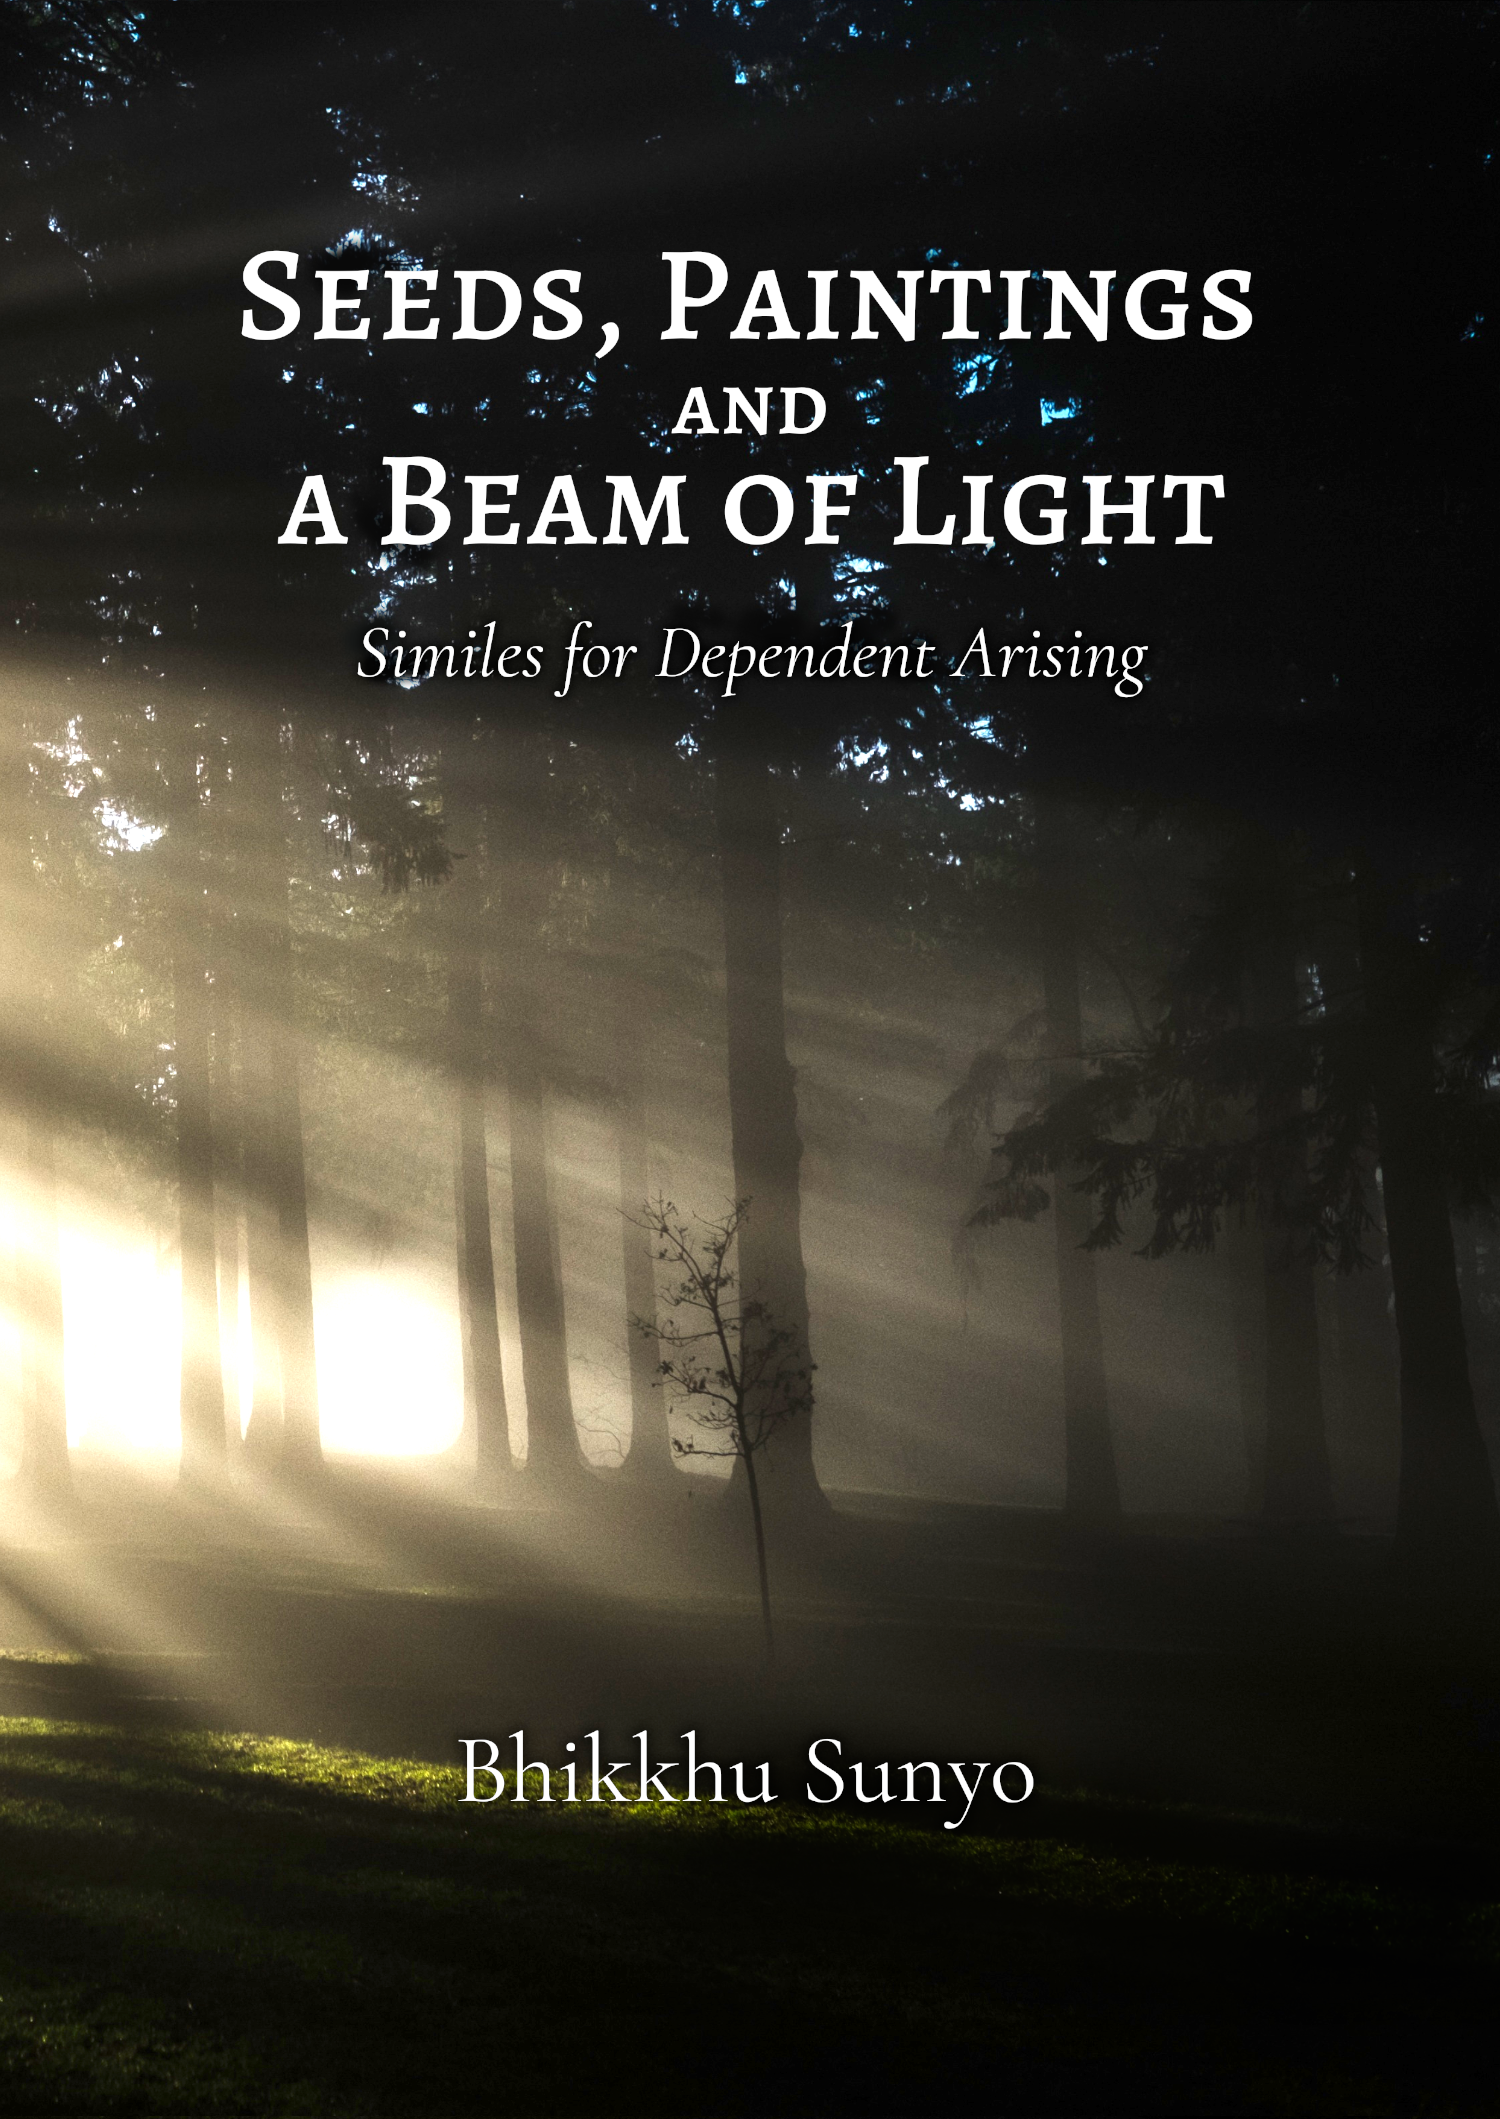
\includegraphics{cover.jpg}

\phantomsection\label{titlepage.xhtml}{}

\phantomsection\label{footprints_split_000.html}{}

\section{}\label{footprints_split_000.html_TOCTarget0-1}

Footprints in the Dust

\emph{The Life of the Buddha from the Most Ancient Sources}

Bhante S. Dhammika

I see him in mind as if by eye\\
And spend the night in praising him;\\
Thus it is I am never away from him.

Sutta Nipāta 1142\\
\href{https://suttacentral.net/snp5.19/en/sujato\#12.1}{Snp\,5.19:12.1--12.4}


\includegraphics{logo-enso-large.png}

Wisdom \& Wonders\\
Books\\
\href{https://wiswo.org/books}{www.wiswo.org/books}

~

~

~

~

~

~

~

~

\phantomsection\label{footprints_split_000.html_calibre_pb_1}

\phantomsection\label{footprints_split_001.html}{}

\section{Foreword}\label{footprints_split_001.html_TOCTarget0-2}

What was the Buddha like as a human being? How did he relate to others?
With great care and an eye for detail, Venerable Dhammika pieces
together the life events we can \textquotesingle read\textquotesingle{}
from very early texts. The result is a truly authoritative biography. It
shows that as a man, as well as a teacher, the historical Buddha was
remarkable indeed. The chapter headings are refreshingly original:~a day
in the life of, his humour, his debating style, his background. I really
enjoyed thinking about Gotama Buddha simply as a person -- and clearly
an extraordinary one, as Ven. Dhammika shows us. I recommend this book
to anyone who would like a down-to-earth, accurate and readable
appraisal of the founder of this great world religion, seen through
modern eyes.

Sarah Shaw\\
Oxford, March, 2021

\phantomsection\label{footprints_split_001.html_calibre_pb_3}

\phantomsection\label{footprints_split_002.html}{}

\section{Preface to the Second
Edition}\label{footprints_split_002.html_TOCTarget0-3}

For this second edition of \emph{Footprints in the Dust} I have included
details about the Buddha and the world he knew which I had previously
overlooked. Also, Stuart Corner and Barry Ng both patiently went through
the original text making many corrections to the spelling and
references, and Bryan Levman drew my attention to aspects of Pali and
the Dhamma that needed clarification and in some cases correction. I am
most grateful to them all for their input. I must also thank Brihas
Sarathy and Steve Hanlon of Pariyatti for arranging this second edition
and seeing it through the press.

\phantomsection\label{footprints_split_002.html_calibre_pb_5}

\phantomsection\label{footprints_split_003.html}{}

\section{Preface}\label{footprints_split_003.html_TOCTarget0-4}

In a sense, I have been writing this book for thirty-five years. Who the
Buddha was and what he was like has intrigued and fascinated me since I
became a Buddhist in my late teens. In my 1989 book \emph{The Buddha and
His Disciples} I looked at some aspects of his persona, his style of
teaching and his relationships, and in the subsequent decades I wrote
several articles dealing with other aspects of the Buddha's life: his
physical appearance, his habits, his travels and even his diet. Some of
that earlier work has been incorporated into the present book. To get at
least some feel for the world in which the Buddha lived, I also
undertook three walking tours through India that followed in his
footsteps: going from Bodh Gaya to Varanasi; from Bodh Gaya to Rajgir
and back again; and, longest of all, retracing the Buddha's final
journey from Rajgir to Kusinara. In the last few years I have also
immersed myself in Vedic literature from both the early and late
periods, the better to understand the religious and social background to
the Buddha's life.

In writing this book I have received generous help and encouragement
from many people. Discussions with Anandajoti Bhikkhu, Peter Prins,
Sarah Shaw and Peter Harvey have been enormously helpful mainly on
matters related to the Dhamma. Input from Bhikkhu Khemarato, Bhikkhunī
Acala, Chris Burke and Ranjith Dissanayake helped fine-tune the final
draft. Bradley Smith and my brother Charles each went through the
manuscript, making numerous corrections and suggestions for its
improvement. Discussions with Deepak Ananda, who shares my deep interest
in the ancient topography of Buddhism, kindly shared his knowledge of
this subject with me. In the end though, I am responsible for everything
in the book. As he has done many times before, Suhendra Sulistyo
arranged for me to get access to books and monographs I needed. In
writing about the Buddha in the time of the coronavirus and serious
personal illness, the good cheer and encouragement of Calvin and Yandi,
Padma, Ananda and Tony have also been much appreciated. I express my
gratitude and thanks to them all.

\phantomsection\label{footprints_split_003.html_calibre_pb_7}

\phantomsection\label{footprints_split_004.html}{}

\section{Note on Usage}\label{footprints_split_004.html_TOCTarget0-5}

The Buddhist scriptures include numerous repetitions that make tedious
reading for those unfamiliar with this genre of literature. I have
condensed these repetitions where necessary, and where this has been
done, it is indicated in the quotes themselves or in the notes. Unless
otherwise mentioned, Pali rather than Sanskrit has been used throughout.
A few exceptions are made to this in deference to widespread usage, the
main ones being Nirvana instead of Nibbāna and stupa rather than thūpa.
In Buddhist literature the conventional way of indicating a large number
of things is to say that there were five hundred. This has been replaced
by `many', `a large number' or `several hundred.' Throughout, `the text'
or `the earliest texts' are used interchangeably with `the Tipitaka.'
Likewise, samaṇa, monk and ascetic are used interchangeably. In Pali as
in Sanskrit, the term `samaṇas and brahmins' is a compound and does not
usually mean both types of individuals but is a conventional way of
referring to religious in general. When referring to the Buddha before
his awakening, he is called by his clan name Gotama, and after his
awakening he is called the Buddha.

\phantomsection\label{footprints_split_004.html_calibre_pb_9}

\phantomsection\label{footprints_split_005.html}{}

\section{\texorpdfstring{{Chapter 1}\\
Introduction}{Chapter 1 Introduction}}\label{footprints_split_005.html_TOCTarget1}

Buddhism teaches that each person comes into their present life from an
earlier one and that most people will have another life when their
present one ends. This process of being born, dying and being reborn is
called \emph{saṃsāra} and only ceases when one attains a state called
awakening, \emph{bodhi}, more commonly known as Nirvana. Like everyone
else, the Buddha had many lives before his final one as Gotama, and the
Buddhist tradition created fictional biographies of over five hundred of
these former lives, recounted in a book called the Jātaka. What is
unique about the Buddha is not that he had former incarnations,
fictional or otherwise, but that in the centuries after he attained
Nirvana devotees and admirers have continued to `reincarnate' him in a
sense, by creating new `lives' for him, some of these more incredible
than his former ones as recounted in the Jātaka.

Although physically and in a number of other ways the Buddha was an
ordinary human being, some participants at the Third Buddhist Council,
which took place around the middle of the second century BCE, asserted
that such was his purity that his faeces had a fragrant smell. There
were, however, those who maintained a more realistic view of the Buddha
and who gave a common-sense rebuttal to this claim. If this were true,
they argued, it would have required the Buddha to eat perfume, and it
was well-known that he ate rice and other ordinary food. Furthermore, if
his faeces really smelled fragrant, people would have collected it,
stored it up and used it as a cosmetic, but there is no record of this
ever being
done.\phantomsection\label{footprints_split_005.html_fnref1}\hyperref[footprints_split_024.htmlux5cux23fn1]{\textsuperscript{1}}

Several centuries after this, a biography of the Buddha called the
\emph{{Lalitavistara
{{[}\hyperref[footprints_split_023.htmlux5cux23Dharmachakraux5cux25202013]{Dharmachakra
2013}{]}}}} depicted him as an individual in whose presence marvels and
wonders manifested, the way mushrooms appear after rain. To give but one
example from many, when as a child he was taken to a temple for a
blessing, the statues of the gods stood up out of reverence for him.

A century or two after this, the \emph{{Saddharmapuṇdarīka Sūtra
{{[}\hyperref[footprints_split_023.htmlux5cux23Robertsux5cux25202022]{Roberts
2022}{]}}}} went much further and maintained that the Buddha was
actually an eternal cosmic being and that the so-called human Buddha was
just an apparition this cosmic Buddha used to teach
humanity.\phantomsection\label{footprints_split_005.html_fnref2}\hyperref[footprints_split_024.htmlux5cux23fn2]{\textsuperscript{2}}
But even as this divine, or quasi-divine, wonder-working Buddha was well
on the way to becoming standard in some quarters, more grounded voices
could still be heard.

One of these was Aśvaghoṣa, who in the early second century CE wrote his
\emph{{Buddhacarita
{{[}\hyperref[footprints_split_023.htmlux5cux23Olivelleux5cux25202008]{Olivelle
2008}{]}}}}, a narrative poem of the Buddha's life from his first to his
last days. In this epic, the Buddha was depicted as exceptional but
still human. In about the sixth century the Hindu \emph{{Matsya Purāṇa
{{[}\hyperref[footprints_split_023.htmlux5cux23Basuux5cux25201916]{Basu
1916}{]}}}} proclaimed that the Buddha was actually an incarnation
(\emph{avatāra}) of the god Visṇu, a claim repeated later by other
\emph{Purāṇas}. This half-hearted effort to neutralize Buddhism by
absorbing it into Hinduism was never really taken seriously by Hindus
and certainly not by Buddhists.

By about the tenth century a confused and fragmentary account of the
Buddha's life had filtered through the Middle East into Europe, and
because it depicted him as conspicuously holy it was assumed that he
must therefore have been a Christian. Consequently, he was inducted into
the Catholic Church as a saint under the name St. Josaphat, with his
feast day being the 27{th} of November.

With the penetration of European powers into Asia, the Buddha underwent
a new wave of `incarnations', finally emerging as an historically real
individual, although it took time to establish that he was not a god, a
prophet of God, and not Chinese but Indian.

By the middle of the Victorian era, he came to be seen by the more
liberal minded as a reformer of Hinduism, a rationalist or a great moral
teacher just one step below Christ; a few bold souls even dared to
suggest that he was equal to
Christ.\phantomsection\label{footprints_split_005.html_fnref3}\hyperref[footprints_split_024.htmlux5cux23fn3]{\textsuperscript{3}}
Some proclaimed that the Buddha was an atheist or an agnostic, while
others were equally sure he believed in God but said little on the
subject because the Divine is beyond words.

In the early 1880s the eminent Dutch scholar of Indian religion Hendrik
Kern published a two-volume tome in which he proved that Buddhism grew
out of sun worship and that the Buddha was originally a solar deity. The
twelve \emph{nidāna} of Buddhist doctrine were the months of the year,
the six wrong views were the six planets, the Buddha's Middle Way was
the summer solstice in disguise, and so on. Although Kern's fellow
academics had great respect for his learning, the sun soon set on his
astronomical theory of the Buddha.

In 1916, just as the distinction between Buddhism and Hinduism was
becoming more apparent, the art historian Ananda Coomaraswamy wrote a
book claiming that the Buddha taught the Ātman and Brahman of Vedānta,
although using different terminology. His book was widely read and
helped perpetuate misunderstandings about Buddhism that continue even
today.

Inspired by the new thinking of the Second Vatican Council, eminent
theologian Karl Rahner informed Buddhists in the late 1950s that they
were actually what he called ``anonymous Christians'' and presumably,
that the Buddha was also a Christian without knowing it. As of today, no
Buddhist thinker has returned the compliment by announcing that
Christians are anonymous Buddhists and that Jesus was really a
late-comer to the Dhamma, despite not wearing a yellow robe.

After the counter-culture movement of the 1960s and the subsequent
emergence of New Age spirituality, the Buddha became an apostle of
vegetarianism who had opened his third eye and taught how to become one
with the universe.

At around the same time, in liberal Christian circles there were those
who were claiming that if Jesus and the Buddha had ever met, they would
have been the best of friends and smilingly nodded in agreement when
each explained their teachings to the
other.\phantomsection\label{footprints_split_005.html_fnref4}\hyperref[footprints_split_024.htmlux5cux23fn4]{\textsuperscript{4}}

Out of step with all these curious, though generally positive,
incarnations, is a recent publication revealing for the first time that
the Buddha was actually an accomplished field general with extensive
experience in commanding men in battle. Apparently he probably
``witnessed so much battlefield carnage that he suffered a psychological
collapse.'' The book also informs the reader that there is ``a
reasonable suspicion'' that the Buddha was
murdered.\phantomsection\label{footprints_split_005.html_fnref5}\hyperref[footprints_split_024.htmlux5cux23fn5]{\textsuperscript{5}}

With so many `Buddhas' it is hardly surprising that in the minds of many
people this Indian sage is a figure hovering between myth and reality,
benign and compelling but not quite real. There are, of course, and have
been for at least a century and a half, studies that present more
realistic or perhaps better, more conventional accounts of the Buddha,
whoever he was and whatever he taught. However, nearly all these
efforts, including contemporary ones, recount the Buddha's biography by
padding the meagre and scattered facts from the earliest sources with
legends that evolved centuries after his passing. And because even the
information from these more reliable early sources is not enough for a
decent-sized volume, at least half or more of such biographies typically
recount the Buddha's philosophy rather than being primarily about the
man himself.

Logically, the best way to know who the Buddha was and what he was like
would be to examine the earliest records of him, simply because they
would be closer to his time than any later ones. Such an endeavour,
however, is not as easy as it sounds. Dating ancient Indian literature
is a notoriously difficult and frustrating task, and there is usually
diverse opinion amongst scholars about when any particular text was
written. Complicating the task even further is that few ancient texts
are homogeneous, with most being written at one time but undergoing
expansion or revision in later centuries. There is, however, a general
consensus amongst scholars that the core material in the Pali Tipitaka,
sometimes also called the Pali Canon, contains the earliest accounts of
the Buddha and what he taught.

The name Tipitaka is a combination of the words \emph{ti}, meaning
`three', which refers to the three divisions of the scriptures, and
\emph{piṭaka}, meaning `a basket.' Calling the scriptures `baskets'
relates to the fact that they were transmitted orally for several
centuries, there being no writing during the Buddha's time. In ancient
India labourers would move earth, grain or building materials using a
relay of large, round, shallow baskets. A worker would put the filled
basket on his head, walk to the next worker, and pass it to him, and
then he would repeat the process. So in the minds of the early
Buddhists, the passing of material in baskets from the head of one
person to another was analogous to passing the scriptures from the
memory of one person to another.

The three divisions of the Tipitaka are the Sutta Piṭaka, the Vinaya
Piṭaka and the Abhidhamma Piṭaka. The first and most important of these
contains the sermons and dialogues of the Buddha, plus a few by his
monastic and lay disciples. Each of these individual sermons and
dialogues is called a \emph{sutta}, meaning a thread or string, and may
have been used because the sounds strung together give the words, and
the words strung together give the meaning. However, \emph{sutta} is
more likely derived from the Sanskrit \emph{sūkta} meaning
well-spoken.\phantomsection\label{footprints_split_005.html_fnref6}\hyperref[footprints_split_024.htmlux5cux23fn6]{\textsuperscript{6}}
These suttas are arranged into five collections, or \emph{nikāya}s, the
fifth of which is made up of thirteen independent books. From the
language, content and style of several books in this fifth collection it
can be deduced that they were composed later than the core material in
the first four collections, and indeed most of them do not even claim to
have been spoken by the
Buddha.\phantomsection\label{footprints_split_005.html_fnref7}\hyperref[footprints_split_024.htmlux5cux23fn7]{\textsuperscript{7}}
It is also true that scattered throughout the first four collections are
some suttas that date from perhaps a century or two after the Buddha,
but for the most part these can be easily identified.

The second part of the Tipitaka, the Vinaya Piṭaka, contains a bare list
of the rules for monks and nuns known as the Pātimokkha and is the
oldest part of the Vinaya. This list of rules is embedded in a
commentary explaining each rule, laying down the procedures for
governing the monastic order and giving the early history of the order.
Parts of this commentary are early and include information about the
Buddha that is likely to be authentic, while other parts were composed a
century or two after the Buddha and are less reliable.

The third part, the Abhidhamma Piṭaka, is a précis of the essential
features of the Buddha's Dhamma, mostly in the form of lists enabling
the Dhamma to be more easily remembered and perhaps more easily taught
as well. The Abhidhamma Piṭaka dates from perhaps two hundred years
after the Buddha, and while it contains little that contradicts his
teaching as presented in the Sutta Piṭaka, it does develop some of these
teachings. However, it contains nothing that could help in constructing
a biography of the Buddha either and has not been used in this book.

The Tipitaka is in an ancient language called Pali which originated in
northern India roughly around the time of the Buddha. The general
opinion amongst scholars about the origin and nature of Pali is that,
``{[}w{]}hile it is not identical to what Buddha himself would have
spoken, it belongs to the same broad language family as those he might
have used and originates from the same conceptual matrix. This language
thus reflects the thought-world that the Buddha inherited from the wider
Indian culture into which he was born, so that its words capture the
subtle nuances of that
thought-world.''\phantomsection\label{footprints_split_005.html_fnref8}\hyperref[footprints_split_024.htmlux5cux23fn8]{\textsuperscript{8}}
However, Prof. Richard Gombrich, the renowned scholar of early Buddhism,
has recently argued against this position, saying that there are cogent
reasons for thinking that the Buddha did speak
Pali.\phantomsection\label{footprints_split_005.html_fnref9}\hyperref[footprints_split_024.htmlux5cux23fn9]{\textsuperscript{9}}
Perhaps the most that can be said is that the Buddha spoke either Pali
or a language quite similar to it.

It is acknowledged that the Tipitaka was assembled in its present form
over a period of probably several centuries and that it is an amalgam of
mostly early material with lesser parts added later. But with a careful
examination of this material, together with intelligent guesswork, it is
possible to identify the earliest stratum within the Tipitaka. Such an
approach reveals that the core material in the Sutta Piṭaka and parts of
the Vinaya Piṭaka dates from the time of the Buddha to perhaps a
generation or two after him.

The \emph{Mañjuśrīmūlakalpa} claims that a decade or so after the
Buddha's passing, King Ajātasattu's son and heir Udāyin, had the
Buddha's words committed to writing (\emph{tadetat pravachanaṃ śāstu
lekhā-payishyati
vistarm}).\phantomsection\label{footprints_split_005.html_fnref10}\hyperref[footprints_split_024.htmlux5cux23fn10]{\textsuperscript{10}}
If this were so, it would seem that the more conservative and
traditional monastic communities who were the majority, continued to
rely on oral transmission. It is commonly thought that written
information is transmitted with greater accuracy than memory, but the
evidence shows otherwise. Before printing, books had to be copied by
hand, and scribes often made mistakes as they wrote. Over time, as one
book was copied from another, mistakes accumulated to the degree that
sometimes it became difficult to work out what some parts of the
original meant. More seriously, a lone scribe could delete or add
passages to the book he was copying, which would be included in the next
copy, creating confusion when compared with manuscripts without the
changes.

Human memory, on the other hand, particularly if trained from childhood
and in a world devoid of all the distractions we are bombarded with, can
be highly accurate, and this is exactly what brahmins, the priests of
India's ancient Vedic religion, did. A brahmin boy was trained from an
early age to repeat the Vedic hymns over and over again until they were
imprinted in his
memory.\phantomsection\label{footprints_split_005.html_fnref11}\hyperref[footprints_split_024.htmlux5cux23fn11]{\textsuperscript{11}}
During various ceremonies, congregations of brahmins chanted the hymns
so that, even if one of them missed a verse or mispronounced a word, his
memory would be jogged or his mistake corrected by the chanting of the
others. This also made it almost impossible for an individual to add or
delete anything once the text was settled and `closed.' To do so would
require a widespread conspiracy, and as the texts came to be considered
sacrosanct, no one would dare to do such a thing.

A significant number of the Buddha's disciples were from the brahmin
caste, and they brought these skills to their new
religion.\phantomsection\label{footprints_split_005.html_fnref12}\hyperref[footprints_split_024.htmlux5cux23fn12]{\textsuperscript{12}}
When someone became a monk, he would listen to the discourses being
chanted and gradually learn them by heart. It is also known that some
monastic congregations specialized in learning different parts of what
became the Tipitaka. To help preserve the Buddha's sermons, they were
edited in ways that made them more amenable to memorisation. They are
replete with mnemonic devices such as numbered lists, stereotyped
passages, standardised terminology, rhyming verses, and, most of all,
repetitions, one of the reasons why it takes time and patience to get
used to their
style.\phantomsection\label{footprints_split_005.html_fnref13}\hyperref[footprints_split_024.htmlux5cux23fn13]{\textsuperscript{13}}
This editing gave the Buddha's sermons a somewhat artificial and stilted
form while still preserving the meaning of what he taught and sometimes
quite likely the very words he spoke. Time and again while reading the
Tipitaka, phrases and short passages stand out as being natural,
unaffected and personal, just the kind of thing a real person would say.
Thus there is no reason to doubt that the core material in the Tipitaka
represents an accurate record of what the Buddha taught as remembered by
his direct disciples and inherited by the immediate succeeding
generation. For a detailed survey of the issues involved and evidence
for the fidelity of the Pali Tipitaka, the reader can consult
\href{https://wiswo.org/books/auth}{\emph{The Authenticity of the Early
Buddhist Texts}} by Bhikkhu Sujato and Bhikkhu Brahmali.

Material evidence of the Buddha is meagre. In the year 249 BCE the
Indian emperor Asoka made a pilgrimage to Gotama's birthplace at Lumbini
and had a huge stone pillar erected there with an inscription on it. The
inscription reads:

\begin{quote}
``Twenty years after his coronation, Beloved-of-the-Gods, King Piyadasi
(i.e. Asoka), visited this place and worshipped because here the Buddha,
the sage of the Sakyans, was born. He had a stone figure and a pillar
erected and because the Lord was born here, the village of Lumbini was
exempted from tax and required to pay only one eighth of the produce.''
\end{quote}

This is the earliest undisputed mention of the Buddha outside the
Tipitaka. Another piece of evidence is an inscribed relic casket found
in a stupa at Piprahwa, the site of Kapilavatthu, Gotama's hometown. The
inscription reads: ``This casket of relics of the blessed Buddha of the
Sakyas {[}is gifted by{]} the brothers Sukirti, jointly with their
sisters, sons and wives.'' Unfortunately, as is so frustratingly common
with ancient Indian records, there is disagreement among scholars about
the age of this inscription. Based on its orthography, some believe it
is earlier than Asoka's inscriptions, but others consider it to be
contemporary with them or even later. The jury is still
out.\phantomsection\label{footprints_split_005.html_fnref14}\hyperref[footprints_split_024.htmlux5cux23fn14]{\textsuperscript{14}}

Another piece of evidence may be a passage from the \emph{Maitrāyaṇīya
Upaniṣad} condemning ``\ldots{} the tawny robed ones who convert others
with rational arguments, examples and the jugglery of a false doctrine
that denies the soul, and who teach a Dhamma that is destructive to the
Vedas\ldots''\phantomsection\label{footprints_split_005.html_fnref15}\hyperref[footprints_split_024.htmlux5cux23fn15]{\textsuperscript{15}}
This Upaniṣad dates from after the Buddha, although not very long after,
and seems to be referring to Buddhist monks and the distinctive Buddhist
doctrine of \emph{anatta}, both of which presuppose the Buddha himself.
\phantomsection\label{footprints_split_005.html_fnref16}\hyperref[footprints_split_024.htmlux5cux23fn16]{\textsuperscript{16}}

There is no chronologically arranged narrative of the Buddha's life in
the Tipitaka as there is, for example, for Jesus in the Gospels or for
Emperor Augustus in \emph{De Vita Caesarum}. However, the Vinaya
includes an account of approximately the first two years of the Buddha's
career, starting with his awakening at Uruvelā up to the conversion and
ordination of the two men who were to become his chief disciples,
Sāriputta and
Moggallāna.\phantomsection\label{footprints_split_005.html_fnref17}\hyperref[footprints_split_024.htmlux5cux23fn17]{\textsuperscript{17}}
This looks like it was the beginning of an attempt to write an account
of the Buddha's life but for some reason it was never completed. The
longest discourse in the Sutta Piṭaka also records the events in the
Buddha's life from the time he left Rājagaha to his death in Kusināra
about twelve months later. These two narratives indicate that, despite
scholarly opinion on the matter, the ancient Buddhists did have a sense
of history and wished to portray the Buddha at a particular time and
place within it. In fact, these two Tipitaka narratives are the earliest
examples from India of an attempt to describe historical events and to
compose a continuous, coherent
story.\phantomsection\label{footprints_split_005.html_fnref18}\hyperref[footprints_split_024.htmlux5cux23fn18]{\textsuperscript{18}}

Nonetheless, it is almost impossible to work out when most of the other
events in the Buddha's career took place during the more than four
decades between these two narratives. Added to this is the fact that the
Tipitaka records almost nothing about the Buddha's life before he became
a wandering ascetic at the age of twenty-nine. Consequently, while we
know a great deal of what the Buddha taught, where he taught it, to whom
he taught it, and sometimes the circumstances that prompted him to teach
it, we know very little at all about exactly when in his life it took
place. Thus a biography of him from birth to death is not
possible.\phantomsection\label{footprints_split_005.html_fnref19}\hyperref[footprints_split_024.htmlux5cux23fn19]{\textsuperscript{19}}

But biographies are more than just an account of chronologically
arranged events. They also include details about their subject's
character, habits, attitudes, achievements and relationships with
others, and the Tipitaka includes a great deal of information about such
things concerning the Buddha, perhaps more than about any other person
from ancient times. Most of this information is in the form of
vignettes, brief asides and tangential comments made in passing, which
makes them all the more compelling because most of them have no
doctrinal value and are therefore likely to be genuine memories of the
people who knew and interacted with the Buddha. When all this material
is put together with what can be inferred about the Buddha from what he
taught, it provides a surprisingly realistic and complete portrait of
the man.

One thing that raises doubts about the value of the Tipitaka for
providing information about the Buddha as a real person is the
supernormal abilities some passages ascribe to him. Examples of this
include him levitating, hearing conversations over a long distance,
reading people's minds, and being visited by and conversing with
heavenly beings. Although the Buddha did have remarkable psychic
abilities, some of those ascribed to him are probably later
embellishments, and it is also likely that many of the people who
interacted with the Buddha genuinely believed that they witnessed him
manifesting such powers. It is well-known that charismatic individuals
are often credited with having superhuman or at least exceptional
abilities, and there is little doubt that the Buddha had a great deal of
personal
charisma.\phantomsection\label{footprints_split_005.html_fnref20}\hyperref[footprints_split_024.htmlux5cux23fn20]{\textsuperscript{20}}
As for the later embellishments, they express a world-view of which
supernormal phenomena were a part. Indeed, it is likely that this very
world-view was partly responsible for the inclusion of such material
into the Tipitaka. That and the prestige this may have given the sermons
in the eyes of the intended audience, are sufficient to explain why they
are there. There is no good reason for thinking that the existence of
these elements shows that the transmission of the core material in the
Tipitaka is
unreliable.\phantomsection\label{footprints_split_005.html_fnref21}\hyperref[footprints_split_024.htmlux5cux23fn21]{\textsuperscript{21}}

\phantomsection\label{footprints_split_005.html_calibre_pb_11}

\phantomsection\label{footprints_split_006.html}{}

\section{\texorpdfstring{{Chapter 2}\\
An Era of
Change}{Chapter 2 An Era of Change}}\label{footprints_split_006.html_TOCTarget2}

\begin{quote}
To the frontier town of Kajaṅgala and nearby Mahāsālā in the east, and
to the Sallavatī River in the south-east, does the Middle Land extend.
To the town of Setakaṇṇika in the south, the brahmin village of Thūna in
the west, and the Usīraddhaja Mountains in the north does the Middle
Land extend.
\end{quote}

Vinaya i, 197\\
\href{https://suttacentral.net/pli-tv-kd5/en/brahmali\#13.12.2}{Kd\,5:13.12.2--13.12.6}

The Buddha was born in and spent his whole life in what was then called
by the people who lived there the Middle Land (\emph{majjhima desa}), an
area roughly equivalent to the modern north Indian states of Bihar and
Uttar Pradesh.

In about the seventh century BCE a discovery was made that was to have a
profound effect on every aspect of life in this region. Iron was
discovered in what is now northern Jharkhand and the hills between Agra
and Gwalior. This metal had been known in India for at least a few
hundred years before this, but the metal now discovered was closer to
the surface and of a higher quality, meaning that it was easier to mine
and smelt. Now every farmer could have an iron tip on his ploughshare
and an iron hoe or spade to turn the earth where his plough could not be
used. Iron sickles made harvesting less laborious, and iron nails held
wooden structures together better. More significantly, it meant that the
forests which covered much of the Middle Land could be cleared more
efficiently, thus opening up more land for agriculture.

Up until this time, most settlements in the Middle Land were small and
on or near rivers; now they gradually became larger and started
appearing in the hinterland. Where once only tribal people and hunters
roamed, now agriculturalists settled and laid out fields. Most of these
settlements grew organically, but there is evidence that kings founded
villages to hasten the development of their kingdoms. One text describes
how a king had a reservoir excavated and cottages built, which
encouraged farmers to move to the site from elsewhere. The ground around
a nearby sacred tree was levelled for as far as its branches extended,
then surrounded by a fence with arched gates so that the new settlers
would have somewhere to
worship.\phantomsection\label{footprints_split_006.html_fnref22}\hyperref[footprints_split_024.htmlux5cux23fn22]{\textsuperscript{22}}
The net result of these changes was a larger food surplus and a
consequent growth in the population, so that small settlements grew into
villages, villages into towns and towns into
cities.\phantomsection\label{footprints_split_006.html_fnref23}\hyperref[footprints_split_024.htmlux5cux23fn23]{\textsuperscript{23}}
For the first time since Mohenjo-Daro, Harappa and Rakhigarhi, the great
cities of the Indus Valley a thousand years earlier, large population
centres became a feature of the landscape of northern India.

The Buddha described a mythical ideal city he called Kusavatī as being
``twelve \emph{yojanas} long from east to west and seven wide from north
to south. It was rich and prosperous, crowded, full of people and with
abundant food \ldots{} Day and night it resounded with the ten sounds;
that of elephants and horses, chariots and drums, tablas and veenas,
singing, cymbals and gongs, and with cries of `Eat, drink, and eat
more.'\,''\phantomsection\label{footprints_split_006.html_fnref24}\hyperref[footprints_split_024.htmlux5cux23fn24]{\textsuperscript{24}}
Although fanciful, parts of this description are clearly based on what
one of the main metropolises the Buddha was familiar with could have
been like.

In the texts, cities are described as having ramparts or walls with
towers at intervals along them, gates, and sometimes as having moats
around
them.\phantomsection\label{footprints_split_006.html_fnref25}\hyperref[footprints_split_024.htmlux5cux23fn25]{\textsuperscript{25}}
Gatekeepers would scrutinize everyone who entered the city and would
patrol the walls to make sure there was no way for anyone to creep in or
out at
night.\phantomsection\label{footprints_split_006.html_fnref26}\hyperref[footprints_split_024.htmlux5cux23fn26]{\textsuperscript{26}}
The east gate was usually considered the most auspicious and therefore
was the main entrance into the city, while the south gate was the most
inauspicious, beyond which was the rubbish dump, the charnel ground or
cremation ground and execution ground. The gates were usually named
after the destination they opened
to.\phantomsection\label{footprints_split_006.html_fnref27}\hyperref[footprints_split_024.htmlux5cux23fn27]{\textsuperscript{27}}

Some of the notable buildings in a city included the king's palace, the
court, the treasury, the tax office and the market. The most important
public buildings in any city or town were the municipal halls, which
usually consisted of an open-pillared structure on a platform.
Typically, there were also alms halls at each city gate, in the centre
of the city, and at the entrance to the king's palace. The most basic of
these halls were provided with benches and water
jars,\phantomsection\label{footprints_split_006.html_fnref28}\hyperref[footprints_split_024.htmlux5cux23fn28]{\textsuperscript{28}}
and during festive occasions or religious events alms would be
distributed from these halls to the poor, the indigent and wandering
ascetics. They also provided shelter for travellers who had nowhere else
to stay and for ascetics who might be passing through. There were also
halls for entertainment (\emph{kutūhala sālā}), which served as venues
for popular events, including religious debates. Queen Mallikā of Kosala
built such a hall next to a line of Tinduka trees in her park in
Sāvatthī, and the Tipitaka records an occasion when some three hundred
ascetics of different sects assembled
there.\phantomsection\label{footprints_split_006.html_fnref29}\hyperref[footprints_split_024.htmlux5cux23fn29]{\textsuperscript{29}}

Most ordinary houses were made of wood, wattle and daub or unfired brick
and roofed with thatch or with tiles for those who could afford them.
The Buddha described a prosperous citizen's residence as ``a peak-roofed
house plastered inside and out and with well-fitted doors and shutters
keeping the draft out. Inside there might be a couch spread with woollen
blankets and covers, a fine antelope skin, with a canopy above and
crimson pillows at either end, an oil lamp burning and four wives
attentive to their master's
pleasure.''\phantomsection\label{footprints_split_006.html_fnref30}\hyperref[footprints_split_024.htmlux5cux23fn30]{\textsuperscript{30}}
Archaeological investigation of early cities such as Rājagaha, Vesālī,
Kosambī and Bhita show that houses typically had two floors and did not
abut each other but always had a small gap between them, probably so
that during fires one house could be cleared without destroying the
adjacent
one.\phantomsection\label{footprints_split_006.html_fnref31}\hyperref[footprints_split_024.htmlux5cux23fn31]{\textsuperscript{31}}

Although there is no mention in the Tipitaka of fires sweeping through
cities or towns, such disasters must have periodically happened, given
that most buildings were of wood, all cooking was done on open fires and
all lighting at night was by lamp. There was a custom, or in some cities
or towns a law, that each household had to have five pots of water
available to fight fires that might break
out.\phantomsection\label{footprints_split_006.html_fnref32}\hyperref[footprints_split_024.htmlux5cux23fn32]{\textsuperscript{32}}
Once, it was reported to the Buddha that the women's quarters in
Kosambī's royal palace had caught fire, resulting in numerous
deaths.\phantomsection\label{footprints_split_006.html_fnref33}\hyperref[footprints_split_024.htmlux5cux23fn33]{\textsuperscript{33}}

As nearly all the cities of the time were on the banks of large rivers,
another danger they were subject to was flooding. Archaeology has
uncovered evidence of massive flooding in Patna, and Hastinapura was
flooded so many times that it was eventually abandoned for several
centuries. It is not surprising that the Buddha frequently mentions fire
and floods as two of the dangers to a family's hard-earned
wealth.\phantomsection\label{footprints_split_006.html_fnref34}\hyperref[footprints_split_024.htmlux5cux23fn34]{\textsuperscript{34}}

With large numbers of people living close to each other and sanitary
arrangements rudimentary at best, another problem cities faced was the
outbreak and spread of disease. What might be one of the few mentions of
such occurrences was when Ānanda informed the Buddha that a monk, a nun
and ten lay disciples had recently died in Nādikā, perhaps because there
had been an epidemic of some kind in the
town.\phantomsection\label{footprints_split_006.html_fnref35}\hyperref[footprints_split_024.htmlux5cux23fn35]{\textsuperscript{35}}

Another feature of the cities was parks and gardens, some of them
private and others open to the public, a few within the cities but most
in their environs. There is evidence that some of these parks included
flowers, bushes and trees planted for ornamental purposes, ponds
beautified with water lilies and lotuses, bowers of flowering creepers,
and benches. The royal pleasure garden in Sāvatthī included an art
gallery (\emph{cittāgāra}) which was open to the public, at least
sometimes.\phantomsection\label{footprints_split_006.html_fnref36}\hyperref[footprints_split_024.htmlux5cux23fn36]{\textsuperscript{36}}
The Veḷuvana, the Bamboo Grove, just beyond the north gate of Rājagaha,
had places where people could come to feed the squirrels and
peacocks.\phantomsection\label{footprints_split_006.html_fnref37}\hyperref[footprints_split_024.htmlux5cux23fn37]{\textsuperscript{37}}
Most of these parks and gardens, however, or at least the ones open to
the public, were just small pockets of forest which had been preserved
as the suburbs expanded. They were popular places for the many ascetics
of the time to lodge or meet with other ascetics or lay folk who were
interested in what they had to say. There are numerous references to the
Buddha or his monastics staying in or spending the day in such parks and
being visited by people wanting to converse with them. Encountering the
Buddha at the Añjana Park at Sāketa, the ascetic Kuṇḍaliya described for
him how he spent his time:

\begin{quote}
``After I have finished my breakfast, it is my habit to amble from one
park or garden to another, and while there I observe various ascetics
and brahmins discussing how they can defend their position during a
debate and criticise the positions of
others.''\phantomsection\label{footprints_split_006.html_fnref38}\hyperref[footprints_split_024.htmlux5cux23fn38]{\textsuperscript{38}}
\end{quote}

The Buddha praised one such place, Rājagaha's Bamboo Grove, as being
``not too near the city, not too far, convenient for coming and going,
quiet, secluded from people, good for sitting without being disturbed
and conducive to spiritual
practice.''\phantomsection\label{footprints_split_006.html_fnref39}\hyperref[footprints_split_024.htmlux5cux23fn39]{\textsuperscript{39}}
So associated were gardens with wandering ascetics of all sects,
including Buddhist monks, that the word \emph{ārāma}, garden or park,
actually took on the double meaning of monastery or hermitage.

There were no temples at this time, but there were religious shrines
(\emph{cetiya}): trees or rock formations in which gods or spirits were
believed to dwell and earthen mounds (\emph{thūpa}, Sanskrit
\emph{stūpa}) raised over the ashes of long dead saints or heroes. The
ashes of Mahāvīra, the leader of the Jains, were interred in a stupa,
and King Muṇda raised a stupa over the ashes of his queen, perhaps
because he had great love and esteem for
her.\phantomsection\label{footprints_split_006.html_fnref40}\hyperref[footprints_split_024.htmlux5cux23fn40]{\textsuperscript{40}}
Vesālī had such shrines at each of the four directions around the city
and at a number of other locations within it. The Buddha once visited
the Maṇimālaka Cetiya in Rājagaha, where the spirit (\emph{yakkha})
Maṇibhadda was believed to
reside.\phantomsection\label{footprints_split_006.html_fnref41}\hyperref[footprints_split_024.htmlux5cux23fn41]{\textsuperscript{41}}
This shrine, much rebuilt and renovated over the centuries, still exists
and is now known as Maniyar Math.

The evidence from Buddhist texts and other contemporary sources
indicates that the cities and towns of the Middle Land supported a
lively civic and cultural life. Philanthropic individuals had large
reservoirs excavated in which people could bathe, wash and do laundry
and from which they could fetch drinking water. These reservoirs were
sometimes lined with stone, had steps leading down into them, and could
be planted with lotuses to beautify them. Vesālī had several such
reservoirs, and the Sumāgandha Pond in Rājagaha was one of the sights of
the city, as was Queen Gaggarā's Lotus Lake in Campā. One Jātaka story
recounts how a wealthy individual endowed his city with what would now
be called a civic centre. After consulting with architects and
designers, he had a complex built with accommodation for travellers, the
homeless and the sick, with one section for males and another for
females. There were venues for sports, for religious activities and for
hearing court cases, and outside the complex was a reservoir with
bathing steps, surrounded by a garden. When the whole complex was
completed, the donor engaged artists to cover all the walls with
paintings.\phantomsection\label{footprints_split_006.html_fnref42}\hyperref[footprints_split_024.htmlux5cux23fn42]{\textsuperscript{42}}
Although this story is perhaps exaggerated, there is little doubt that
the wealthy sometimes did establish such places.

Poetry was already a highly developed art, and recitals took place in
small groups and at various public gatherings. The Buddha had some
interest in and knowledge of poetry. He was familiar with poets
composing in four different genres, conversant with prosody, and
mentioned that the most popular hymn was the
\emph{sāvittī}.\phantomsection\label{footprints_split_006.html_fnref43}\hyperref[footprints_split_024.htmlux5cux23fn43]{\textsuperscript{43}}
His appreciation of poetry was probably the reason why some of his
disciples were either accomplished poets or became so, e.g. Vaṅgīsa, who
composed a series of beautiful verses in praise of the Buddha, and also
Ambapālī, India's first poetess.

It was common to see itinerant entertainers in city streets -- pole
acrobats, snake charmers, magicians and minstrels. Brief references to
actors, dancers, mimes and bards, and of performers' managers, suggests
that such entertainment had reached a sophisticated
level.\phantomsection\label{footprints_split_006.html_fnref44}\hyperref[footprints_split_024.htmlux5cux23fn44]{\textsuperscript{44}}
Every year in Rājagaha there was an event called the Hilltop Festival
(\emph{giraggasamajja}), at which there was much eating, drinking and
theatrical
performances.\phantomsection\label{footprints_split_006.html_fnref45}\hyperref[footprints_split_024.htmlux5cux23fn45]{\textsuperscript{45}}
Occasionally there also seems to have even been something like informal
beauty pageants, where the winner would be designated the fairest in the
land. The Buddha described crowds of people jostling each other to see
such a winner and urging her to sing and dance for
them.\phantomsection\label{footprints_split_006.html_fnref46}\hyperref[footprints_split_024.htmlux5cux23fn46]{\textsuperscript{46}}

The cows that wandered through city streets could sometimes injure or
even kill people, as happened to Bāhiya just after his discussion with
the Buddha. To minimize this hazard, cattle would sometimes have their
horns
removed.\phantomsection\label{footprints_split_006.html_fnref47}\hyperref[footprints_split_024.htmlux5cux23fn47]{\textsuperscript{47}}
It was normal to throw human waste, rubbish and food scraps into the
streets which were as a result, odorous, dirty and usually only cleaned
just before
festivals.\phantomsection\label{footprints_split_006.html_fnref48}\hyperref[footprints_split_024.htmlux5cux23fn48]{\textsuperscript{48}}
We read of ``the drains and rubbish heaps in the alleys'' at
Kusinārā.\phantomsection\label{footprints_split_006.html_fnref49}\hyperref[footprints_split_024.htmlux5cux23fn49]{\textsuperscript{49}}
With no street lighting, being out at night, especially late, could be
problematic and was something the Buddha advised his disciples to
avoid.\phantomsection\label{footprints_split_006.html_fnref50}\hyperref[footprints_split_024.htmlux5cux23fn50]{\textsuperscript{50}}
Walking through a city or town in the dark, one might fall into a
cesspit or sewer, stumble over a sleeping cow, or encounter delinquents
intent on crime or a prostitute offering to expose herself for a small
coin.\phantomsection\label{footprints_split_006.html_fnref51}\hyperref[footprints_split_024.htmlux5cux23fn51]{\textsuperscript{51}}

Occasional civil disturbances were not unknown either. There is a
mention of a minor riot over a prostitute by a group of youths and
widespread public drunkenness during some
festivals.\phantomsection\label{footprints_split_006.html_fnref52}\hyperref[footprints_split_024.htmlux5cux23fn52]{\textsuperscript{52}}
Occasionally some of the wandering ascetics of the time would come into
the cities and towns to try to get some basic necessities, like cast-off
clothes, salt, medicine or just food. They could be seen standing at
doors with their alms bowls or sitting at strategic locations with their
hands out asking for alms.

While the new and growing cities and towns in the Middle Land could have
large populations, the majority of people still lived in villages. The
inhabitants of most villages were farmers, although the texts have
frequent references to villages of potters, fisherman, reed-cutters,
smiths, salt makers and carpenters, reflecting the division of labour
that was taking place at the time. Typically, a village would be
surrounded by a fence, sometimes of mud bricks, wood or thorny tree
branches as a protection against wild animals and thieves, and be
entered through a
gate.\phantomsection\label{footprints_split_006.html_fnref53}\hyperref[footprints_split_024.htmlux5cux23fn53]{\textsuperscript{53}}
The village's boundary, which included its fields and common land, were
also clearly defined, to avoid conflicts with neighbouring villages and
for taxation
purposes.\phantomsection\label{footprints_split_006.html_fnref54}\hyperref[footprints_split_024.htmlux5cux23fn54]{\textsuperscript{54}}
The repetition and drudgery of the farmer's life was described by the
Buddha's cousin Anuruddha like this: ``Having brought in the crop,
exactly the same thing has to be done the next year and exactly the same
the year after that. The work never ends; there is no end in sight to
it.''\phantomsection\label{footprints_split_006.html_fnref55}\hyperref[footprints_split_024.htmlux5cux23fn55]{\textsuperscript{55}}

Burdensome taxation, banditry and, worst of all, the vagaries of the
weather meant that life was hard for rural folk. While the ancient law
books stipulated that a fair tax on the harvest should range from a
sixth to a twelfth, in reality rulers, whether kings or council elders,
could raise as much revenue as they wanted, on top of imposing levies
and charges for numerous other
things.\phantomsection\label{footprints_split_006.html_fnref56}\hyperref[footprints_split_024.htmlux5cux23fn56]{\textsuperscript{56}}
But it was the unpredictability of the weather that posed the greatest
threat. A drought might cause food shortages for city-dwellers, but it
could mean death for rural folk. The texts mention a famine in Kāsi
because of the monsoon's failure three years in a row, so that the land
looked ``as if scorched by
fire.''\phantomsection\label{footprints_split_006.html_fnref57}\hyperref[footprints_split_024.htmlux5cux23fn57]{\textsuperscript{57}}
The Buddha spoke of how a drought in one region would cause hungry
people to flee to another region, where they would have to live in
crowded conditions in what we would call refugee
camps.\phantomsection\label{footprints_split_006.html_fnref58}\hyperref[footprints_split_024.htmlux5cux23fn58]{\textsuperscript{58}}
Even when the monsoons were late by only a week or two, people would be
haunted by what were called the three fears (\emph{tīṇi bhayāni}): fear
of drought, of famine and of
disease.\phantomsection\label{footprints_split_006.html_fnref59}\hyperref[footprints_split_024.htmlux5cux23fn59]{\textsuperscript{59}}
And in a cruel irony, sometimes it was not lack of rain causing the
problem but too much, so that the subsequent floods destroyed crops,
resulting in
famine.\phantomsection\label{footprints_split_006.html_fnref60}\hyperref[footprints_split_024.htmlux5cux23fn60]{\textsuperscript{60}}
Someone once asked the Buddha why in the past the population was large
enough that ``villages, towns and royal capitals were so close together
that a rooster could fly from one to another,'' whereas now there were
far fewer people. He replied that peoples' excessive greed had caused
civil strife, droughts and malevolent spirits, all of which had made the
population
decline.\phantomsection\label{footprints_split_006.html_fnref61}\hyperref[footprints_split_024.htmlux5cux23fn61]{\textsuperscript{61}}
As the Buddha saw it, ``life is short, limited and fleeting, and only
rarely does anyone live to a
hundred.''\phantomsection\label{footprints_split_006.html_fnref62}\hyperref[footprints_split_024.htmlux5cux23fn62]{\textsuperscript{62}}

The Buddha observed that if a man had been away from his village for an
extended period and he were by chance to meet another man from his
village, he would anxiously ask whether things back home were safe,
whether there had been any epidemics, food shortages or attacks by gangs
of bandits; such was the precariousness of rural
life.\phantomsection\label{footprints_split_006.html_fnref63}\hyperref[footprints_split_024.htmlux5cux23fn63]{\textsuperscript{63}}
So that his disciples would not become complacent, the Buddha asked them
to occasionally reflect that, while now the harvests were good and food
plentiful, this situation could easily change, and thus they should make
full use of the good times to practise the
Dhamma.\phantomsection\label{footprints_split_006.html_fnref64}\hyperref[footprints_split_024.htmlux5cux23fn64]{\textsuperscript{64}}

Of course, life could not have been all work and want, at least not for
everyone, everywhere and all the time. There were occasional
opportunities for relaxation and revelry, even at religious events. The
Buddha spoke of one such religious gathering that took place in the
southern districts, which included food and drink, singing, dancing and
music.\phantomsection\label{footprints_split_006.html_fnref65}\hyperref[footprints_split_024.htmlux5cux23fn65]{\textsuperscript{65}}
Also, he said that with good government the land could be at peace, and
banditry could be suppressed so that happy people, with joyful hearts,
would be able to dance with their children in their arms and keep their
homes
unlocked.\phantomsection\label{footprints_split_006.html_fnref66}\hyperref[footprints_split_024.htmlux5cux23fn66]{\textsuperscript{66}}

City folk tended to consider villagers to be unsophisticated boors and
looked upon them with a degree of contempt. In ordinary parlance the
term \emph{gamma}, `of the village', meant something low and crude. In
keeping with this common usage the Buddha described sexual intercourse,
going to see various spectacles and idle chatter to be ``\emph{gamma}.''
Although the deeper and more philosophical aspects of the Buddha's
teachings would have held little interest for the average villager, his
moral and social teachings certainly did, and it was probably these
aspects of the Dhamma that he taught during his tours, when he would
often stay in villages.

The increasing food surplus, the growth in population and the rise of
cities stimulated another major change in the Middle Land, and that was
the expansion of commerce and the beginning of long-distance and
transcontinental trade. Previously, village communities were almost
entirely self-sufficient, growing their own food and having most of
their other necessities made by local craftsmen. Their few other
essentials they obtained from neighbouring villages, from the nearby
forest or from the occasional peddler or small-time trader who passed
through with his donkey or bullock cart. Exchange was mainly by barter.

There are numerous references in the Tipitaka to caravans of wagons
carrying goods from one city or region to another. While the Buddha was
still at Uruvelā just after his awakening, he met the two merchants
Tapussa and Bhallika who were from Ukkalā, probably somewhere in
Orissa.\phantomsection\label{footprints_split_006.html_fnref67}\hyperref[footprints_split_024.htmlux5cux23fn67]{\textsuperscript{67}}
The texts do not mention these two men being attached to a caravan, but,
coming from such a long distance, they would have been. The wealthy
businessman and patron of the Buddha, Anāthapiṇḍaka, travelled from his
home base in Sāvatthī to Rājagaha and back on business and had a
business estate in
Kāsi.\phantomsection\label{footprints_split_006.html_fnref68}\hyperref[footprints_split_024.htmlux5cux23fn68]{\textsuperscript{68}}
There is mention of several hundred wagons carrying jars of sugar along
the main road between Rājagaha and Andhakavinda, and when the Buddha
rested at the foot of a tree while on his way to Kusinārā, a caravan of
carts forded a nearby
stream.\phantomsection\label{footprints_split_006.html_fnref69}\hyperref[footprints_split_024.htmlux5cux23fn69]{\textsuperscript{69}}
Caravans would sometimes halt in one location for months, acting as a
trading post for districts in the vicinity. The Jātaka includes a story
about a young merchant whose caravans travelled ``now from east to west,
and now from north to
south.''\phantomsection\label{footprints_split_006.html_fnref70}\hyperref[footprints_split_024.htmlux5cux23fn70]{\textsuperscript{70}}
One wagon in his caravan carried large clay jars of water for when
passing through areas where no water was available, and at night the
wagons would be arranged in a circle for protection. A similar story
tells of a caravan that passed through a desert, probably Rajasthan's
Thar Desert, so hot that the caravan could only travel at night, and the
pilot navigated by the
stars.\phantomsection\label{footprints_split_006.html_fnref71}\hyperref[footprints_split_024.htmlux5cux23fn71]{\textsuperscript{71}}

Kings and chiefdom administrations set up custom posts at river
crossings, mountain passes and city gates to collect fees from caravans.
Special government officials manned customs posts and were sometimes
ensconced in large caravans to make sure they paid duty at the
designated
places.\phantomsection\label{footprints_split_006.html_fnref72}\hyperref[footprints_split_024.htmlux5cux23fn72]{\textsuperscript{72}}
Once, the Buddha scolded a monk for being the beneficiary of a fraud
because he had travelled with a merchant's caravan knowing that it
intended to bypass a customs post and thereby avoid paying
duty.\phantomsection\label{footprints_split_006.html_fnref73}\hyperref[footprints_split_024.htmlux5cux23fn73]{\textsuperscript{73}}
We read of merchants from a handful of countries meeting together to
elect a president, probably to establish an international trading house,
and of a city providing a place where foreign merchants could
temporarily store their
goods.\phantomsection\label{footprints_split_006.html_fnref74}\hyperref[footprints_split_024.htmlux5cux23fn74]{\textsuperscript{74}}
The Buddha characterized such merchants and traders as always thinking:
``I will get this from here and that from
there.''\phantomsection\label{footprints_split_006.html_fnref75}\hyperref[footprints_split_024.htmlux5cux23fn75]{\textsuperscript{75}}

Merchants and craftsmen formed guilds (\emph{seṇi} or \emph{pūga}) to
oversee and protect their interests. Traditionally, there were said to
be eighteen guilds, and their presidents or aldermen had direct access
to the king or the ruling council and sometimes even held the position
of finance minister. The Buddha mentions guilds conducting courts to
arbitrate disputes between their
members.\phantomsection\label{footprints_split_006.html_fnref76}\hyperref[footprints_split_024.htmlux5cux23fn76]{\textsuperscript{76}}

Concurrent with the growth in trade, the first currency in India
appeared in perhaps 600 BCE: countable units of copper, silver and gold
coins, with punch marks rather than legends. The standard denomination
was the \emph{kahāpaṇa}, and these were issued by trading houses, guilds
and
governments.\phantomsection\label{footprints_split_006.html_fnref77}\hyperref[footprints_split_024.htmlux5cux23fn77]{\textsuperscript{77}}
The use of money created professions such as accounting, auditing and
calculating (\emph{mudda}, \emph{gaṇanā, saṅkhā}) which, along with
trade and farming, the Buddha considered legitimate
livelihoods.\phantomsection\label{footprints_split_006.html_fnref78}\hyperref[footprints_split_024.htmlux5cux23fn78]{\textsuperscript{78}}

Beyond village-based producers such as carpenters, smiths, potters and
basket weavers, the Tipitaka mentions other workers and craftsmen which
suggest the existence of disposable income and the demand for luxurious
non-essentials. These include goldsmiths, jewellers, ivory-workers,
garland-makers and florists, silk weavers, coach-builders, confectioners
and perfumers. One much sought-after luxury was the embroidered fabric
known as Kāsi cloth manufactured in Bārāṇasī and which the Buddha
described as having a beautiful colour, being pleasant to the touch, and
so valuable that even when it was worn out it was used to wrap gems in
or kept in a scented chest. He also mentioned that as a layman his
turban, tunic, waist cloth and wrap-around scarf were all made of Kāsi
cloth.\phantomsection\label{footprints_split_006.html_fnref79}\hyperref[footprints_split_024.htmlux5cux23fn79]{\textsuperscript{79}}
There were assessors (\emph{agghakāraka}) who valued elephants, horses,
precious stones, gold and other high-priced articles for royal courts
and the affluent, artists who did paintings on the walls of buildings,
on cloth and on polished wooden panels, and weavers who made silk cloth
with gems sewn into
it.\phantomsection\label{footprints_split_006.html_fnref80}\hyperref[footprints_split_024.htmlux5cux23fn80]{\textsuperscript{80}}

Products were imported into the Middle Land from far beyond it: horses
from Sindh; sandalwood from south India; a type of crimson coloured
blanket and wine from Gandhāra; fine Siveyyaka cloth from Sivi; and
conch shells from the far south, to name but a few. The Tipitaka also
mentions high-value, low-volume items such as pearls, beryl, lapis
lazuli, quartz, red coral, ruby and cat's-eye, most of which also made
their way into the Middle Land by way of
trade.\phantomsection\label{footprints_split_006.html_fnref81}\hyperref[footprints_split_024.htmlux5cux23fn81]{\textsuperscript{81}}
The Buddha opined that trading was a livelihood which had certain
advantages over more traditional ones such as farming:

\begin{quote}
``Agriculture is an occupation with much to do, many duties, much
forethought, great problems and which, if it succeeds, yields great
profit\ldots{} Trading is an occupation which requires little work,
fewer duties, planning and problems, and if successful yields greater
profit.''\phantomsection\label{footprints_split_006.html_fnref82}\hyperref[footprints_split_024.htmlux5cux23fn82]{\textsuperscript{82}}
\end{quote}

Like much else in the Middle Land during the sixth to fourth centuries
BCE, momentous changes were also taking place in politics. The few
details recorded in the Tipitaka enable us to say that the old republics
or chiefdoms (\emph{saṅgha} or \emph{gaṇa}) were gradually giving way to
monarchies (\emph{rājaka}). The main kingdoms were Magadha, Kosala,
Vaṃsā and Pañcāla, and the chiefdoms were the Vajjian confederacy and
those of the Mallas, Cedis, Videhas, Koliyas, and the Buddha's clan the
Sakyas, all of them small.

While kings could rule as they liked, restrained perhaps to some extent
by precedent and tradition, the chiefdoms had participatory governments,
although this was only open to the men of high-status families. The
Mallas of Kusinārā for example, had a governing body of eight
counsellors
(\emph{pāmokkha}).\phantomsection\label{footprints_split_006.html_fnref83}\hyperref[footprints_split_024.htmlux5cux23fn83]{\textsuperscript{83}}
The chiefdoms' cities, towns and even villages had council halls where
the business of the state or the community was conducted. The Buddha was
invited by the Mallas of Pāvā to inaugurate their new council hall by
spending the night in
it.\phantomsection\label{footprints_split_006.html_fnref84}\hyperref[footprints_split_024.htmlux5cux23fn84]{\textsuperscript{84}}
Apparently it was considered auspicious to have a revered person `open'
such buildings by doing this.

One text describes how the gods conducted business in their celestial
council hall, which gives a clue to the way such assemblies were
conducted in their earthly equivalent. The participants were seated in a
specific order; after the chairman had presented business to the
assembly, others spoke on the issues involved, and then there was more
voting and discussion until a majority or a unanimous decision was
reached.\phantomsection\label{footprints_split_006.html_fnref85}\hyperref[footprints_split_024.htmlux5cux23fn85]{\textsuperscript{85}}
Terms such as party or faction (\emph{vagga}), party whip
(\emph{gaṇapūraka}), motion (\emph{ñatti}), arbitration
(\emph{ubbāhikā}), constituency (\emph{sīmā}), referendum
(\emph{yebhuyyasikā}), and rules of the council (\emph{sabhādhamma})
indicate that there were accepted procedures for conducting such
assemblies. In some councils at least, ballot tickets, literally
`sticks' (\emph{salākā}), were used to cast votes (\emph{chandaka}), and
there could be open voting (\emph{vivaṭaka}) or secret voting
(\emph{gūḷhaka}). The Buddha adopted many of the procedures and rules of
the chiefdoms in the running of the monastic Saṅgha. Less formal were
the town and village meeting days (\emph{negamassa samayo}) presided
over by the headman (\emph{gāmaṇī}), at which the population would
gather and discuss matters concerning their general
welfare.\phantomsection\label{footprints_split_006.html_fnref86}\hyperref[footprints_split_024.htmlux5cux23fn86]{\textsuperscript{86}}

There are references to some of the kingdoms going to war with each
other but none of the chiefdoms doing so. Before Gotama's birth, or
perhaps during his childhood, King Vaṅka of Kosala had invaded and
annexed Kāsi. Later records say that the Sakyan country was incorporated
into Kosala after a swift and bloody campaign, probably within a few
years of the Buddha's demise. The most aggressive kingdom of the time
was Magadha, which had already annexed Aṅga, again probably during
Gotama's youth. Later, when Ajātasattu was on the throne of Magadha, he
invaded Kāsi, initially defeating Kosala's army but then being driven
out by a Kosalan
counter-attack.\phantomsection\label{footprints_split_006.html_fnref87}\hyperref[footprints_split_024.htmlux5cux23fn87]{\textsuperscript{87}}
The Tipitaka has a brief reference to Ajātasattu strengthening
Rājagaha's fortifications, fearing that King Pajjota of Avanti might
invade and, in the last months of the Buddha's life, of him building
fortifications at Pāṭaligāma in preparation for a planned conflict with
the
Vajjians.\phantomsection\label{footprints_split_006.html_fnref88}\hyperref[footprints_split_024.htmlux5cux23fn88]{\textsuperscript{88}}
Within a century of the Buddha's passing, Magadha emerged as the
paramount power, firstly in northern India and eventually in most of the
subcontinent.

It is hard to know how large or destructive these and the few other
inter-state conflicts were, but even brief skirmishes could have been
bloody, as the Buddha's comments on war testify. He spoke of how ``men
take up swords and shields, buckle on bows and quivers, and both sides
fling themselves into battle and, with arrows flying, knives waving and
swords flashing, they pierce with arrows, wound with knives and
decapitate with swords and so suffer death or death-like
pain.''\phantomsection\label{footprints_split_006.html_fnref89}\hyperref[footprints_split_024.htmlux5cux23fn89]{\textsuperscript{89}}
He also described how a soldier might ``lose heart, falter or be unable
to brace himself'' on seeing even the dust thrown up by the opposing
army's approach and how those besieging a fortress or city could be
``splashed with boiling oil or crushed by heavy objects'' thrown down on
them.\phantomsection\label{footprints_split_006.html_fnref90}\hyperref[footprints_split_024.htmlux5cux23fn90]{\textsuperscript{90}}

The process whereby a chief might transform himself firstly into a
despot and eventually into a monarch is unclear but it probably happened
through irregular or contested means. The political systems in most of
the chiefdoms were not like Athenian democracy but were rather
oligarchic, where certain elites or families dominated political power.
Nevertheless, an unpopular chief, even though duly elected, might have
to bend to popular opinion or risk being overthrown.

This was the world Gotama was born into, although it is unlikely that he
was aware of much of it until he became a wandering ascetic, his
homeland being on the outer edge of and relatively uninfluenced by much
of what was going in the rest of northern India.

\phantomsection\label{footprints_split_006.html_calibre_pb_13}

\phantomsection\label{footprints_split_007.html}{}

\section{\texorpdfstring{{Chapter 3}\\
Gods, Brahmins and
Ascetics}{Chapter 3 Gods, Brahmins and Ascetics}}\label{footprints_split_007.html_TOCTarget3}

The majority of people in the Middle Land during the Buddha's time were
not Hindus, as is commonly supposed, but rather animists. Because this
animism was an informal, unstructured religion, it has left few traces
of its presence, but something of it can be culled from Brahminical,
Jain and Buddhist sources and to some degree from contemporary Indian
folk religion.

There were no temples at this time, but there were shrines to various
gods and spirits or sometimes revered kings, heroes or people deemed
saintly. The Buddha observed that ``many people go for help to sacred
hills, groves, trees and
shrines.''\phantomsection\label{footprints_split_007.html_fnref91}\hyperref[footprints_split_024.htmlux5cux23fn91]{\textsuperscript{91}}
People believed that the spirits who inhabited such places or the energy
emanating from them had a protective power or would respond to the
prayers or offerings made at them. Milk and water were poured on the
roots of sacred trees, garlands were hung on the branches, lamps of
scented oil were burned around them, and cloth was tied around their
trunks.\phantomsection\label{footprints_split_007.html_fnref92}\hyperref[footprints_split_024.htmlux5cux23fn92]{\textsuperscript{92}}
A type of red or ochre-coloured paste (\emph{vaṇṇaka}) would be smeared
on shrines and flowers placed before
them.\phantomsection\label{footprints_split_007.html_fnref93}\hyperref[footprints_split_024.htmlux5cux23fn93]{\textsuperscript{93}}
There is mention of animal and occasionally even human sacrifices being
made to sacred trees. The victim's blood was poured around the foot of
the tree, and the entrails were draped over the
branches.\phantomsection\label{footprints_split_007.html_fnref94}\hyperref[footprints_split_024.htmlux5cux23fn94]{\textsuperscript{94}}
As today, the trees that were most likely to be inhabited by gods were
pipal trees or banyan trees, particularly old and majestic ones.

The belief in and worship of various spirits, such as \emph{yakkhas}
(and their female equivalents \emph{yakkhinīs}), \emph{bhūtas},
\emph{nāgas}, \emph{rakkhasas}, \emph{kumbhaṇḍas}, \emph{pisācas} and
\emph{picācillikās} was also common. These beings lurked in cemeteries,
remote stretches of forests and along lonely roads and encountering one
at night would be enough to make one's hair stand on
end.\phantomsection\label{footprints_split_007.html_fnref95}\hyperref[footprints_split_024.htmlux5cux23fn95]{\textsuperscript{95}}
Some were benevolent, but more usually they were menacing and had to be
propitiated with offerings of flowers and incense or, for the more
malevolent ones, with meat and
alcohol.\phantomsection\label{footprints_split_007.html_fnref96}\hyperref[footprints_split_024.htmlux5cux23fn96]{\textsuperscript{96}}
A yakkha, a type of ogre, could possess people, which was a ``fierce,
terrible and horrifying'' experience, causing the victim to cry out in
alarm: ``This yakkha has possessed me, harmed and hurt me, and will not
let me
go!''\phantomsection\label{footprints_split_007.html_fnref97}\hyperref[footprints_split_024.htmlux5cux23fn97]{\textsuperscript{97}}
One later text says that yakkhas named Kāla and Upakālaka were
worshipped in Kapilavatthu, the Buddha's
hometown.\phantomsection\label{footprints_split_007.html_fnref98}\hyperref[footprints_split_024.htmlux5cux23fn98]{\textsuperscript{98}}
Nāgas were semi-aquatic beings inhabiting deep lakes or lonely jungle
pools. They could adopt a human form one minute and a serpent-like one
the next. Generally kindly when treated with respect, nāgas could
quickly change if crossed and kill with their poisonous breath or
incinerate with their laser-like gaze.

Gods (\emph{devas}) were seen as being in some sense separate from and
higher than the various spirits. Pāṇini made a distinction between the
`official' gods of the Vedas and worldly (\emph{laukika}) gods of folk
beliefs, such as earth spirits (\emph{bhumā
devā}).\phantomsection\label{footprints_split_007.html_fnref99}\hyperref[footprints_split_024.htmlux5cux23fn99]{\textsuperscript{99}}
But by the fifth century BCE it was becoming more difficult to separate
the two, as Brahminism gradually assimilated many local deities into its
pantheon, usually by claiming that they were a different `aspect' of a
Vedic god or simply a god's alternative name. Many of the local or
regional gods and goddesses were associated with fertility, rain and the
protection of crops. Some of the more popular of these, such as Śri, the
goddess of good fortune, and Vessavaṇa, the king of the directional
gods, were later merged into the Hindu pantheon as Lakshmi and Kubera.

The formal religion during the Buddha's time was Brahminism, which, in
the centuries after the Buddha, gradually morphed into Hinduism. Those
who practiced this religion were known as Vedists (\emph{vaidika}).
Brahminism had a priesthood, a canon of scriptures, a liturgical
language, and various clearly defined doctrines and rituals. Its sacred
texts were the three Vedas --- the \emph{Ṛgveda}, \emph{Yajurveda} and
the \emph{Sāmaveda} --- with the first of these being the oldest and
most important. A collection of spells, incantations and magical charms
called the \emph{āthabbaṇa} was known to the Buddha in the fifth century
BCE and came to be accepted as a fourth Veda, the \emph{Artharvaveda},
some centuries
later.\phantomsection\label{footprints_split_007.html_fnref100}\hyperref[footprints_split_024.htmlux5cux23fn100]{\textsuperscript{100}}

The Vedas consist of hymns addressed to various gods, praising them and
calling upon them for help. The most popular of these gods were
Pajāpati, Soma, Indra, Yama and Agni, although there were many others.
The sacrifices (\emph{yāga}) during which the hymns were chanted were
the central sacrament of Brahminism. They were elaborate rituals
conducted by a number of brahmin priests and arranged by a sponsor
hoping to gain wealth, progeny, the love of a woman, victory over rivals
or other worldly gains from one or another of the gods. The sacred fires
that were the focus of the sacrifice were ignited, and offerings of
ghee, milk, grain, cakes and flowers were thrown into the flames and
carried aloft to the gods in the smoke. There were sacrifices marking
the passing of the seasons, to consecrate rulers, to ward off calamity,
to bring rain, to guarantee victory in war and for a hundred other
matters. In more important sacrifices, animals were slaughtered and
offered to the fire. The Buddhist texts describe one such sacrifice in
which hundreds of bulls, bullocks, heifers, goats and rams were
slaughtered.\phantomsection\label{footprints_split_007.html_fnref101}\hyperref[footprints_split_024.htmlux5cux23fn101]{\textsuperscript{101}}
During other sacrifices a hallucinogenic drink called soma was consumed
by the brahmins and shared with the gods, although by the fifth century
BCE the plant from which this drink was made seems to have disappeared.
There were also much smaller and less elaborate domestic sacrifices
which were done daily in the home and conducted by the family.

Vedic Brahminism had its origins perhaps a thousand years before the
Buddha, beyond the western edge of the Middle Land in what is now
northwestern Pakistan and adjoining areas of Afghanistan. This region
was called Āryāvarta, and its inhabitants were a semi-nomadic people who
called themselves Aryans (\emph{āryas}), noble ones. One of the most
notable features of the Aryan's religion was the belief that humans were
of four different kinds: brahmins or priests; warriors
(\emph{khattiya}); traders/farmers (\emph{vessa}); and menials
(\emph{sudda}, Sanskrit \emph{śūdra}). Below these groups were
forest-dwelling peoples who were beyond the pale of Aryan society and
were considered untouchables. The first three castes were called
twice-born (Sanskrit \emph{dvija} or \emph{dvijāti}) because at a
certain age a male underwent an initiation rite which cemented him into
his caste and its practices and obligations; but the fourth caste, the
menials, could not participate in any Vedic rituals, and untouchables
and foreigners had no place in Brahminical religion at all. According to
the \emph{Ṛgveda}, each caste had been created from different parts of
Pajāpati's body: the brahmins from his mouth; warriors from his arms;
traders/farmers from his thighs; and the menials from his
feet.\phantomsection\label{footprints_split_007.html_fnref102}\hyperref[footprints_split_024.htmlux5cux23fn102]{\textsuperscript{102}}
No explanation was offered for the origins of the untouchables.

To the Aryans, the people of the Middle Land to their east were demonic
and ``as stupid as cows'' because they did not follow Aryan customs,
worship the Vedic gods or honour
brahmins.\phantomsection\label{footprints_split_007.html_fnref103}\hyperref[footprints_split_024.htmlux5cux23fn103]{\textsuperscript{103}}
According to some Brahminical texts it was improper to perform the
sacrifice in the east, i.e. the Middle Land. Worse still, Easterners
were lax in their practice of caste, the cornerstone of the Vedic social
order, and thus were ritually impure. Nevertheless, for several
centuries the Aryans had been gradually moving east, bringing their
culture and religion with them, so that by the Buddha's time Brahminism
was on the way to being integrated into the culture of the Middle Land,
transforming it and, to some extent, being transformed by it. Brahmins
recommend themselves to kings and local rulers, giving them legitimacy,
offering to perform rituals that could guarantee victory in war, regular
rainfall and male progeny; and acting as administrators and advisors. In
return, they were granted estates and certain privileges, and their
social theories, particularly the fourfold division of society, were
given theoretical justifications that led them to becoming accepted as
the norm. The Buddhist scriptures mention both brahmins living in their
own villages and of brahmins coming ``from the north,'' implying that
they were purer and more ritually potent having come from the Āryavata
rather than in the inferior Middle Land.

Over the centuries, and certainly by the Buddha's time, the meaning of
the Vedic sacrifice had changed and, with it, how the ritual was
performed. The hymns came to be seen more as magical spells that, if
pronounced absolutely correctly, would compel the gods to grant
requests. What had been relatively simple rituals became increasingly
complex and expensive and entailed significant amounts of offerings
being thrown into the sacred fire. The fees brahmins required for
performing these and other rituals had also become exorbitant. The
growing dissatisfaction with these changes resulted in some people, at
least, beginning to reinterpret certain Brahminical doctrines, a trend
reflected in the early \emph{Upaniṣad}s, and encouraged an openness to
the broader religious culture of the Middle Land.

Brahminism was very much a community-centred, family-orientated
religion. The ideal setting for the twice-born's life was living amongst
his kin in a village, and his goal was to have a faithful wife who could
give him sons and to be rich in land and cattle. The new cities that
were sprouting up were repugnant to brahmins. One text states: ``They
say that a man who disciplines himself well will attain final bliss even
though he lives in a city, with his body, hands and face covered with
its dust. But this is
impossible!''\phantomsection\label{footprints_split_007.html_fnref104}\hyperref[footprints_split_024.htmlux5cux23fn104]{\textsuperscript{104}}
A similar attitude is echoed in another text: ``He should avoid a main
city as he would\ldots the boiling caldron of
hell.''\phantomsection\label{footprints_split_007.html_fnref105}\hyperref[footprints_split_024.htmlux5cux23fn105]{\textsuperscript{105}}
Some brahmins even maintained that the sacrifice would not work if it
was performed in a city. Brahminism was a religion of the countryside;
as we shall see, Buddhism was more a religion of towns and cities.

Not a religion as such, but a religious movement which had a presence
throughout the Middle Land, probably for centuries already before the
Buddha's time, was that of a class of ascetics most commonly called
\emph{samaṇas}.\phantomsection\label{footprints_split_007.html_fnref106}\hyperref[footprints_split_024.htmlux5cux23fn106]{\textsuperscript{106}}
These ascetics were also known variously as wanderers
(\emph{paribbājaka}), because of their homelessness; ford-makers
(\emph{titthakara}), because they were endeavouring to find or claimed
to have found a way to cross the raging river of conditioned existence;
mendicants (\emph{bhikkhu} or \emph{piṇḍola}), because they begged for
alms; or silent ones (\emph{muni}), for their penchant for being quiet
and retiring. As well as being itinerant and mendicant, most samaṇas
were also celibate. The Buddha said of the typical samaṇa that, ``having
accepted sufficient alms, he goes his way, as a bird, when it flies here
or there, takes nothing with it but its
wings.''\phantomsection\label{footprints_split_007.html_fnref107}\hyperref[footprints_split_024.htmlux5cux23fn107]{\textsuperscript{107}}
He described his senior disciple Sāriputta as an ideal samaṇa because he
was one ``with few wishes, contented, secluded, solitary, energetic and
devoted to developing the higher
mind.''\phantomsection\label{footprints_split_007.html_fnref108}\hyperref[footprints_split_024.htmlux5cux23fn108]{\textsuperscript{108}}
Although most samaṇas were males, there were smaller numbers of females
who had chosen the life of renunciation. According to which sect they
belonged to, some of these women wore their hair in a topknot. Having
men and women in the same group together could lead to problems, and the
Buddha reported some male wandering ascetics saying: ``Real happiness is
the downy soft arms of a female
wanderer.''\phantomsection\label{footprints_split_007.html_fnref109}\hyperref[footprints_split_024.htmlux5cux23fn109]{\textsuperscript{109}}

It has been argued that the samaṇa tradition was a response to
disaffection and alienation caused by the new urbanization taking place
at this time and thus that it was a recent phenomenon, but it is more
likely that it was an ancient tradition indigenous to the Middle Land.
Others have argued that Buddhism started as a reaction against
Brahmanism but this theory is increasingly being called into question
too.\phantomsection\label{footprints_split_007.html_fnref110}\hyperref[footprints_split_024.htmlux5cux23fn110]{\textsuperscript{110}}

In contrast to the brahmins, the samaṇas generally rejected the Vedas
and most Brahminical beliefs and practices and gave precedence to
personal experience over dogma and scriptural authority. They
experimented with meditation, self-mortification, yogic breathing,
fasting and extended periods of isolation. The two movements also
aspired to different goals. Brahminism was concerned with success in
this world and heaven in the next, while the samaṇas renounced all
worldly concerns, believing that some forms of ecstatic mystical
experience were achievable either here and now or after death. A few
samaṇas, however, taught a materialist philosophy or were sceptical of
all philosophical viewpoints, and, of the seven most prominent teachers
of the time, none of them taught a form of monotheism.

A samaṇa who believed he had attained some kind of spiritual realization
might attract disciples, and thus a sect or school would come into
being; others lived in small, informal bands, and a few lived alone in
forests. According to which discipline or ideology they subscribed to,
there were samaṇas who went naked, symbolic of their rejection of all
social norms and values, while others wore animal skins or robes made
out of rags, usually dyed tawny brown or yellow. Some shaved their
heads, others tore their hair out, and still others let their unkempt
hair grow so that it formed matted dreadlocks.

By the fifth century BCE, there were at least a dozen major samaṇa
fraternities or sects in the Middle Land, such as the Muṇḍaka Sāvakas,
the Jatilas, the Māgaṇḍka, the Tedaṇḍikas,~the Aviruddhakas and the
Devadhammikas. Samaṇa teachers who were attracting attention included
Pūraṇa Kassapa, Ajita Kesakambalī, Pakudha Kaccāyana, Sañjaya
Belaṭṭhaputta, Mahāvīra, and, of course, the two teachers who guided
Gotama's early explorations, Āḷāra Kālāma and Uddaka
Rāmaputta.\phantomsection\label{footprints_split_007.html_fnref111}\hyperref[footprints_split_024.htmlux5cux23fn111]{\textsuperscript{111}}
Most of these sects, their founders and the doctrines they espoused soon
faded into obscurity and were forgotten. Other than the Buddhists, the
only ones to last more than a few centuries were the Ājīvakas and the
Jains, then known as the Nigaṇṭhas, the Bondless
Ones.\phantomsection\label{footprints_split_007.html_fnref112}\hyperref[footprints_split_024.htmlux5cux23fn112]{\textsuperscript{112}}

The Ājīvakas had been founded by Makkhali Gosāla, who had originally
been a companion of Mahāvīra, the Jain leader, before falling out with
him and starting his own movement. Only a few scattered and partly
contradictory references to Gosāla's doctrine survive, but it seems to
have been a kind of rigid determinism and included many magical
practices. The Buddha's repudiation of such practices, particularly
astrology, was probably an indirect criticism of the Ājīvaka teachings.
The Ājīvakas garnered considerable support for a few centuries and then
went into a long period of decline, finally disappearing in about the
thirteenth
century.\phantomsection\label{footprints_split_007.html_fnref113}\hyperref[footprints_split_024.htmlux5cux23fn113]{\textsuperscript{113}}

Jainism had been founded by the sage Pārśva in about the seventh century
BCE, and was then reformed, reformulated and revitalized by Mahāvīra,
the Buddha's older contemporary, called Nātaputta in the Buddhist texts.
Those who adhered to Pārśva's original doctrine and discipline still
existed during the Buddha's time and, outwardly at least, differed from
Mahāvīra's disciples, who went naked, by wearing a small cloth over
their genitals -- hence their name, `They of the One Cloth'
(\emph{ekasātaka}).\phantomsection\label{footprints_split_007.html_fnref114}\hyperref[footprints_split_024.htmlux5cux23fn114]{\textsuperscript{114}}
Their leader, Keśin, accepted an invitation to meet with a senior
disciple of Mahāvīra to discuss their differences, which were eventually
resolved, resulting in the two branches of the religion agreeing to
unite. Apparently, a large crowd of ascetics of different sects had
gathered to listen to the
discussion.\phantomsection\label{footprints_split_007.html_fnref115}\hyperref[footprints_split_024.htmlux5cux23fn115]{\textsuperscript{115}}

Despite being the two most prominent teachers of the time and their
disciples often engaging in polemics with each other, it is strange that
Mahāvīra and the Buddha never met. It is stranger still to learn that on
occasions they stayed in the same location at the same time -- for
example once in Vesālī and on another occasion in Nāḷandā -- and that
they both spent the same three months of a rainy season in Rājagaha, and
yet never took the opportunity to meet and debate their respective
views.\phantomsection\label{footprints_split_007.html_fnref116}\hyperref[footprints_split_024.htmlux5cux23fn116]{\textsuperscript{116}}
It would appear that neither man wanted a face to face encounter with
the other.

In many respects Jainism was similar to Buddhism, but a major
difference, and one from which several other differences arise, was the
idea in Jainism that every act, intentional or not, created
kamma.\phantomsection\label{footprints_split_007.html_fnref117}\hyperref[footprints_split_024.htmlux5cux23fn117]{\textsuperscript{117}}
It also accepted the reality of a soul, something which Buddhism
rejected. Jainism has survived in India until today, and although its
adherents have always been small in number, they have had a profound and
positive influence on Indian thought and culture.

By the Buddha's time a small but significant number of brahmins had
adopted some samaṇa practices, particularly renunciation, forest living
and meditation. Known as \emph{vānaprastha} or \emph{vaikhānasa}, they
were usually identified by their matted hair (\emph{jaṭila}) and the
deer skins (\emph{ajina}) they
wore.\phantomsection\label{footprints_split_007.html_fnref118}\hyperref[footprints_split_024.htmlux5cux23fn118]{\textsuperscript{118}}
However, seemingly unable to completely let go of worldly life as
traditional samaṇas did, some spent the day at the edge of their village
or in the nearby forest tending the sacred fire and returned to their
homes in the evening, while others lived permanently in the forest but
kept their wives and children with them. The layman Potaliya thought of
himself as a true renouncer because, although living at home, he had
handed over all his property and obligations to his sons and was content
with being fed and clothed by them. Nonetheless, he became irritated
when the Buddha kept addressing him as ``householder'' during a
conversation the two had, and protested that he was no longer a layman
but a renunciant. The Buddha told him that being a genuine renunciant
required much more than
that.\phantomsection\label{footprints_split_007.html_fnref119}\hyperref[footprints_split_024.htmlux5cux23fn119]{\textsuperscript{119}}

The life of renunciation was such a threat to Brahmanism's theology and
values that the \emph{{Baudhāyana Dharmasūtra
{{[}\hyperref[footprints_split_022.htmlux5cux23Olivelleux5cux25201999]{Olivelle
1999}{]}}}} claimed that it was actually a demonic plot to deprive the
gods of the sustenance they received from sacrificial offerings and thus
destroy them. It would be centuries before renouncing family and society
became fully accepted as a part of
Hinduism.\phantomsection\label{footprints_split_007.html_fnref120}\hyperref[footprints_split_024.htmlux5cux23fn120]{\textsuperscript{120}}

Most samaṇa fraternities or sects looked back to founders who they
believed had lived in the distant past, some of whom were mythical and
others possibly real. As mentioned above, the Jains looked back to
Pārśva. The Buddha once mentioned six ``ford makers'' from the past
whose names were still recalled with
reverence.\phantomsection\label{footprints_split_007.html_fnref121}\hyperref[footprints_split_024.htmlux5cux23fn121]{\textsuperscript{121}}
He saw himself as the most recent of these previously awakened Buddhas,
who had rediscovered and reformulated the essence of their teachings. He
explained it like this:

\begin{quote}
``Suppose a man wandering through the forest were to see an ancient road
or path traversed by people in days gone by and he were to follow it
until he came to an ancient city once inhabited by people, with parks
and groves; reservoirs and walls---a really beautiful place. Then that
man would inform the king or one of his ministers about it and say,
`Sir, restore that city!', and they would, and in time it would become
rich and prosperous, crowded and full of people, so that it would grow
and flourish again. In the same way I saw an ancient road or path
traversed by fully awakened Buddhas in the past. And what is that
ancient path, that ancient road? It is the Noble Eightfold
Path.''\phantomsection\label{footprints_split_007.html_fnref122}\hyperref[footprints_split_024.htmlux5cux23fn122]{\textsuperscript{122}}
\end{quote}

The Buddha's immediate predecessor was Kassapa Buddha, again possibly a
real person although with legends built around his life and doctrines
attributed to him which he may or may not have promulgated. The Tipitaka
even contains a few verses supposedly spoken by this Kassapa
Buddha.\phantomsection\label{footprints_split_007.html_fnref123}\hyperref[footprints_split_024.htmlux5cux23fn123]{\textsuperscript{123}}

Although most people treated samaṇas with respect and sometimes even
with awe, not everyone did. The attitude of a few was: ``I cook, but
they don't. It is not right that I who cook should give to those who do
not.''\phantomsection\label{footprints_split_007.html_fnref124}\hyperref[footprints_split_024.htmlux5cux23fn124]{\textsuperscript{124}}
When a samaṇa stood at someone's door waiting for alms, the lady of the
house might politely refuse him, pretend not to see him so she did not
have to give him anything, coolly dismiss him with leftovers, or send
him away with a hail of
abuse.\phantomsection\label{footprints_split_007.html_fnref125}\hyperref[footprints_split_024.htmlux5cux23fn125]{\textsuperscript{125}}
According to the Buddha: ``Being an alms-gatherer is the lowest of
callings. To say, `You are an alms-gatherer, wandering about bowl in
hand' is an insult in today's
world.''\phantomsection\label{footprints_split_007.html_fnref126}\hyperref[footprints_split_024.htmlux5cux23fn126]{\textsuperscript{126}}

Not all samaṇas were worthy of respect either. There are places in the
Tipitaka where the Buddha berated those samaṇas who preyed on people's
devotion or gullibility by claiming to be able to predict the future and
interpret dreams and omens, or who practiced astrology, or dispensed
nostrums ``while living off food provided by the
faithful.''\phantomsection\label{footprints_split_007.html_fnref127}\hyperref[footprints_split_024.htmlux5cux23fn127]{\textsuperscript{127}}
One of the people the Buddha was having a discussion with described the
discourses of many ordinary ascetics and brahmins as nothing more than
chitter chatter (\emph{vilāpaṃ}
\emph{vilapitaṃ}).\phantomsection\label{footprints_split_007.html_fnref128}\hyperref[footprints_split_024.htmlux5cux23fn128]{\textsuperscript{128}}
A few samaṇas were prepared to pander to the powerful in the hope of
obtaining their patronage, and for their part the powerful were not
averse to using samaṇas for their own ends. Because samaṇas travelled
widely and were generally trusted, or at least thought of as innocuous,
they made useful informants and spies. King Pasenadi actually admitted
to the Buddha that he employed certain samaṇas, or people disguised as
them, to gather intelligence for
him.\phantomsection\label{footprints_split_007.html_fnref129}\hyperref[footprints_split_024.htmlux5cux23fn129]{\textsuperscript{129}}
On the whole, though, most samaṇas lived simple, harmless lives
dedicated to the quest for ultimate freedom, even if they never achieved
it.

Given the samaṇas' rejection of the Vedas and the respect they received,
it is not surprising that the more orthodox followers of Brahminism,
particularly brahmin priests, regarded them as rivals, heretics and as
little more than outcastes. The Tipitaka records numerous incidents of
brahmins belittling samaṇas, the Buddha and his monks included. The
antagonism between the two was highlighted by Patañjali (circa. 150
BCE), who wrote that samaṇas and brahmins were ``like cat and mouse, dog
and fox, snake and mongoose,'' meaning that they were polar opposites in
both their lifestyles and their approaches to spirituality. He added
that ``the opposition between the two is
eternal.''\phantomsection\label{footprints_split_007.html_fnref130}\hyperref[footprints_split_024.htmlux5cux23fn130]{\textsuperscript{130}}
While this was not always the case, these observations do point to the
tension and competitiveness between the two, which is reflected in the
literature of the time, including the Tipitaka.

From the beginning, the Buddha saw himself firmly within the samaṇa
tradition and his Dhamma as antithetical to Brahmanism, not a reform of
or a restatement of it, but an alternative to it. When he embarked on
his quest for truth he did not seek out a brahmin teacher to study the
Vedas with, rather he seems to have taken it for granted that the way of
the samaṇas would lead him to the goal he aspired to. Throughout the
Tipitaka the Buddha is addressed as or referred to as ``the samaṇa
Gotama,'' and he asked his monks to identify as samaṇas too. ``Samaṇa,
samaṇa, that is how people perceive you. So when you are asked, `What
are you?' you should reply that you are
samaṇas.''\phantomsection\label{footprints_split_007.html_fnref131}\hyperref[footprints_split_024.htmlux5cux23fn131]{\textsuperscript{131}}
He either rejected, reinterpreted, criticized or ignored almost every
Brahmanical doctrine and practice. He even forbade his Dhamma being
rendered into Sanskrit, mainly so it would be understandable to everyone
but probably also so it could maintain its non-Vedic
distinctiveness.\phantomsection\label{footprints_split_007.html_fnref132}\hyperref[footprints_split_024.htmlux5cux23fn132]{\textsuperscript{132}}

\phantomsection\label{footprints_split_007.html_calibre_pb_15}

\phantomsection\label{footprints_split_008.html}{}

\section{\texorpdfstring{{Chapter 4}\\
The
Sakyans}{Chapter 4 The Sakyans}}\label{footprints_split_008.html_TOCTarget4}

My lineage is Ādicca, I am Sakyan by birth,\\
and it is from this family I have gone forth.

Sutta Nipāta 423\\
\href{https://suttacentral.net/snp3.1/en/sujato\#19.1}{Snp\,3.1:19.1--19.4}

Paralleling the Himalayan foothills that define the modern India-Nepal
border is a strip of terrain called the Terai. The whole region is flat,
and the soil is a rich fertile alluvium. The numerous rivers and streams
that flow down from the hills to the north sink into the gravel and then
percolate to the surface in the Terai, creating pools, marshes and
swamps. For centuries most of the Terai was made up of thick malarial
forest, but beginning in the late nineteenth century it has been
deforested and given over to rice cultivation. To get some idea of what
it was like before the deforestation, one has to visit the Katarniaghat
and the Suhelva sanctuaries, Dudhwa National Park or Valmiki National
Park. Elephants, one-horned rhinoceros, the beautiful chital deer,
tigers, leopards, monkeys, wild buffalo and hyenas roam through stands
of sal, rosewood, khair, champak and bahera trees and areas of tall
grasses. During the monsoon, when the rain has washed the dust from the
atmosphere, the snowy peaks of the Himalayas can be clearly seen on the
horizon to the north.

In the fifth century BCE one of the ethnic groups who inhabited parts of
the Terai were the Sakyans, and it was into this group that the person
who was to become the historical Buddha was born. Nothing in the early
texts suggests that the Sakyan homeland was anything other than a small
and unimportant chiefdom, and it would never have become famous or even
been remembered had the Buddha not been born
there.\phantomsection\label{footprints_split_008.html_fnref133}\hyperref[footprints_split_024.htmlux5cux23fn133]{\textsuperscript{133}}
In a number of places in the Tipitaka sixteen of the main states in the
Middle Land are listed, but Sakya is not amongst them. The Tipitaka also
records the names of a mere ten villages in the Sakyan country, again
suggesting that it covered a modest area and probably that it was
sparsely
populated.\phantomsection\label{footprints_split_008.html_fnref134}\hyperref[footprints_split_024.htmlux5cux23fn134]{\textsuperscript{134}}

The Sakyans claimed to be descendants of the sons of the semi-mythical
King Okkāka, who had been driven into exile by the machinations of his
second
queen.\phantomsection\label{footprints_split_008.html_fnref135}\hyperref[footprints_split_024.htmlux5cux23fn135]{\textsuperscript{135}}
Wandering through the forest, they came to the hermitage of the sage
Kapila who invited them to settle down nearby. Out of gratitude to him,
they named the settlement they established Kapilavatthu, which became
the Sakyan's principal town. Because this settlement happened to be in a
grove of \emph{sāka} trees, the exiles became known as Sakyans -- at
least that's what Sakyan clan history
said.\phantomsection\label{footprints_split_008.html_fnref136}\hyperref[footprints_split_024.htmlux5cux23fn136]{\textsuperscript{136}}
The name Sakya, sometimes Sākya, is more likely to be derived from
\emph{śak}, meaning ``to be able'' or ``capable.'' The Sakyans also
claimed to be of the Ādicca lineage, which supposedly went back to the
Vedic sun god, and to be of the warrior caste.

Although nominally independent, the Sakyans were under the influence of
the kingdom of Kosala, their larger and more powerful neighbour to the
south and west. The Tipitaka says: ``The Sakyans are vassals of the king
of Kosala; they offer him humble service and salutation, do his bidding
and pay him
homage.''\phantomsection\label{footprints_split_008.html_fnref137}\hyperref[footprints_split_024.htmlux5cux23fn137]{\textsuperscript{137}}
This explains why the Sakyan land, ``the land of {[}the Buddha's{]}
birth'' (\emph{jātibhūmaka}), was described as belonging to the king of
Kosala and why the king once said to the Buddha that the two of them
were
Kosalans.\phantomsection\label{footprints_split_008.html_fnref138}\hyperref[footprints_split_024.htmlux5cux23fn138]{\textsuperscript{138}}
One text mentions the king being driven into Sakyan territory in his
state carriage to the town of Medaḷumpa, which would have only happened
if he had suzerainty over the
Sakyans.\phantomsection\label{footprints_split_008.html_fnref139}\hyperref[footprints_split_024.htmlux5cux23fn139]{\textsuperscript{139}}
Tradition says that, towards the end of the Buddha's life\textbf{,} or
more likely after his death, the Sakyans' \emph{de jure} independence
came to an end when their lands were formally absorbed into Kosala.

The Sakyans' neighbors to their east were the Koliyans. The border
between their territories was the Rohiṇī River which has its source in
the Himalayan foothills and flows into the Rapti River a little west of
the modern town of Gorakhpur. A later, although plausible, legend claims
that, during a summer drought, the Sakyans and Koliyans nearly came to
blows over the use of the water in this river, an argument which was
later arbitrated by the
Buddha.\phantomsection\label{footprints_split_008.html_fnref140}\hyperref[footprints_split_024.htmlux5cux23fn140]{\textsuperscript{140}}
The Tipitaka preserves only a few scraps of information about the
Koliyans: the Buddha visited the chiefdom on a few occasions; they had a
form of government similar to that of the Sakyans; they had a kind of
police force which had a distinctive uniform and a reputation for
extortion and high-handedness; and they were one of the claimants for
the Buddha's ashes after he
died.\phantomsection\label{footprints_split_008.html_fnref141}\hyperref[footprints_split_024.htmlux5cux23fn141]{\textsuperscript{141}}
Later texts also claim that the Sakyans were related to and sometimes
intermarried with the Koliyans, which again seems quite plausible.

The Sakyans had a reputation for pride and impulsiveness and were
considered rustics by their neighbours. A group of Sakyan youths are
reported as saying of themselves, ``We Sakyans are proud,'' and Upāli,
himself a Sakyan, described them as ``a fierce people.'' Taking a more
positive stance, the Buddha said his kinsmen were ``endowed with wealth
and
energy.''\phantomsection\label{footprints_split_008.html_fnref142}\hyperref[footprints_split_024.htmlux5cux23fn142]{\textsuperscript{142}}
When an arrogant young brahmin complained to the Buddha that during a
visit to Kapilavatthu the Sakyan youths did not give him due respect,
the Buddha defended his kinsmen, saying: ``But even the quail, such a
little bird, can talk as she likes in her own
nest.''\phantomsection\label{footprints_split_008.html_fnref143}\hyperref[footprints_split_024.htmlux5cux23fn143]{\textsuperscript{143}}
The Buddha's comparison of Sakyans with a little bird is further
evidence of their country's diminutive size and unimportance.

There are only a few scattered references to what the main Sakyan town
Kapilavatthu was like. There was some kind of school and a council hall
(\emph{santhāgāra}) where the elders of the clan would meet to discuss
matters pertaining to the running of the chiefdom. The texts mention
that after the construction of a new council hall and the Buddha was
invited to inaugurate it by spending the night in it: ``the floor was
spread;
\phantomsection\label{footprints_split_008.html_fnref144}\hyperref[footprints_split_024.htmlux5cux23fn144]{\textsuperscript{144}}
seats were arranged; a large pot of water was put out; and an oil lamp
was hung
up.''\phantomsection\label{footprints_split_008.html_fnref145}\hyperref[footprints_split_024.htmlux5cux23fn145]{\textsuperscript{145}}
Within walking distance of Kapilavatthu was the Nigrodhārāma, a park
where the Buddha would stay during his occasional visits. From there he
could walk to the Mahāvana, the Great Forest, indicating that the town
was surrounded on some sides by this extensive forest which reached into
the Himalayan foothills and stretched all the way to Vesālī and probably
beyond.\phantomsection\label{footprints_split_008.html_fnref146}\hyperref[footprints_split_024.htmlux5cux23fn146]{\textsuperscript{146}}
Another place where he would sometimes stay was the mango orchard owned
by the Vedhañña family, of whom nothing else is
recorded.\phantomsection\label{footprints_split_008.html_fnref147}\hyperref[footprints_split_024.htmlux5cux23fn147]{\textsuperscript{147}}
Although Kapilavatthu was almost certainly a small town, one of the few
detailed references to it describes it as being ``rich and prosperous,
crowded and full of people, its streets busy,'' which seems to suggest
that it was something more than a small
place.\phantomsection\label{footprints_split_008.html_fnref148}\hyperref[footprints_split_024.htmlux5cux23fn148]{\textsuperscript{148}}
Archaeology can help resolve the apparent disparity between these two
descriptions.

In the 1980s archaeologists conducted surveys of ancient settlement
sites in the Kanpur district of Uttar Pradesh dating from between the
seventh to the third century BCE. They found eighty-one settlements of
less than two hectares and calculated that these could have had a
population of not more than 500 people. There were fourteen settlements
covering an area of between two and four hectares, and these could have
had a population of between 500 and 1000. Four settlements were more
than four hectares and could have accommodated between 1,200 and 1,300
inhabitants.\phantomsection\label{footprints_split_008.html_fnref149}\hyperref[footprints_split_024.htmlux5cux23fn149]{\textsuperscript{149}}
All these population centres were much smaller than the main cities of
the time, and they would qualify as villages today. If Kapilavatthu had
a population of 1,300, it would have been big enough to be described as
bustling and crowded, especially if it was also a centre of commerce and
the seat of government. Excavations conducted at the site of
Kapilavatthu in the early 1970s confirm the impression that it was a
modest place. They revealed that the area it took up was small, although
the whole site could not be explored because some of it was under
cultivation. All structures dating from the Buddha's time had mud walls,
while those made of baked brick were from a much later period.
Kapilavatthu was nothing like the grand royal capital as described in
later Buddhist
legend.\phantomsection\label{footprints_split_008.html_fnref150}\hyperref[footprints_split_024.htmlux5cux23fn150]{\textsuperscript{150}}
Numerous contemporary biographies of the Buddha repeat the inaccuracy
that Kapilavatthu was in the Himalayan foothills. In fact, the terrain
around it is as flat as it is possible to be; the first line of hills
only starts about thirty kilometres further
north.\phantomsection\label{footprints_split_008.html_fnref151}\hyperref[footprints_split_024.htmlux5cux23fn151]{\textsuperscript{151}}

It has been said that ``the Buddha was born, grew up and died a Hindu,''
a claim apparently based on the assumption that because most Indians
today are Hindus, they must have been in ancient times
too.\phantomsection\label{footprints_split_008.html_fnref152}\hyperref[footprints_split_024.htmlux5cux23fn152]{\textsuperscript{152}}
In reality, we have no idea what religion prevailed amongst the Sakyans
and thus might have influenced the young Gotama. Certainly, there is
little evidence of a brahmin presence in the Sakyan country. Only one
village in the chiefdom, Khomadussa, had some brahmins living in it, and
when the Buddha visited the place they gave him a cool
reception.\phantomsection\label{footprints_split_008.html_fnref153}\hyperref[footprints_split_024.htmlux5cux23fn153]{\textsuperscript{153}}

As mentioned above, Brahminism, the precursor of Hinduism, had been
moving from its traditional sacred land into the Ganges Valley for at
least three hundred years and was in the process of establishing itself
in the region. Kings such as Bimbisāra of Magadha had taken some
brahmins as court advisors and functionaries, but on the other hand one
of his cousins had become an Ājīvaka ascetic, suggesting that some of
the elite were maintaining their allegiance to the non-Vedic samaṇa
tradition.\phantomsection\label{footprints_split_008.html_fnref154}\hyperref[footprints_split_024.htmlux5cux23fn154]{\textsuperscript{154}}
Peoples such as the Sakyans, who were on the fringes of the major
states, were probably still relatively uninfluenced by Brahminism. This
is probably why, when the four castes are mentioned in the Tipitaka, the
warrior caste is always placed before the brahmin caste. This suggests
that the clan-based chiefdoms were still either resisting or ignoring
the brahmin concept of caste hierarchy. The only hint we have of the
religious life of the Sakyans is the brief comment that the Buddha's
uncle Vappa was a follower of the non-Vedic
Jains.\phantomsection\label{footprints_split_008.html_fnref155}\hyperref[footprints_split_024.htmlux5cux23fn155]{\textsuperscript{155}}
The majority of Sakyans, like most people in the Middle Land, were
probably what would now be called animists worshipping their own local
spirits and gods.

We have some information about the political life of the Sakyans. Legend
claims that the Buddha's father Suddhodana was a king, although there is
scant evidence in the Tipitaka to back up this claim. Nowhere is the
Buddha called a prince (\emph{rājakumāra}), nowhere is he or his family
said to live in a
palace,\phantomsection\label{footprints_split_008.html_fnref156}\hyperref[footprints_split_024.htmlux5cux23fn156]{\textsuperscript{156}}
and only once is his father called \emph{rāja}, a word usually
translated as
king.\phantomsection\label{footprints_split_008.html_fnref157}\hyperref[footprints_split_024.htmlux5cux23fn157]{\textsuperscript{157}}
Although by the fifth century this word had come to be used for kings,
in the Buddha's time it still retained its earlier meaning of an elected
chief or consul, without any regal connotations. In one ancient text he
is described as a \emph{virāṭ} which can mean something like head, ruler
or
premier.\phantomsection\label{footprints_split_008.html_fnref158}\hyperref[footprints_split_024.htmlux5cux23fn158]{\textsuperscript{158}}
Even in the very places where one would expect the Buddha to call his
father a king or himself a prince, he did not do so. For example, when
asked by King Bimbisāra about his birth and kin, he simply replied that
he was from a Sakyan
family.\phantomsection\label{footprints_split_008.html_fnref159}\hyperref[footprints_split_024.htmlux5cux23fn159]{\textsuperscript{159}}
The Tipitaka says that the Sakyans had a body of men called
`chief-makers' (\emph{rājakattāra}). Such groups are mentioned in other
early Indian texts, and it is clear they elected a chief to rule over
them, either for a set period or for as long as he had their confidence.
\phantomsection\label{footprints_split_008.html_fnref160}\hyperref[footprints_split_024.htmlux5cux23fn160]{\textsuperscript{160}}
The council hall the Buddha had inaugurated in Kapilavatthu was the very
kind of place where the chief-makers and clan elders would gather to
conduct business, with the chief presiding over their meetings as
\emph{primus inter
pares}.\phantomsection\label{footprints_split_008.html_fnref161}\hyperref[footprints_split_024.htmlux5cux23fn161]{\textsuperscript{161}}
So while the Buddha was almost certainly from a ruling class family, he
was not royalty in the sense that came to be understood in later
centuries, or as it is today.

Suddhodana had two wives, Mahāmāyā, Gotama's mother, and her sister
Mahāpajāpatī Gotamī, although whether they were co-wives or he married
the latter after the death of the former cannot be determined. Sororate
marriages were recognized in ancient India and are mentioned in later
law books. The second part of Mahāmāyā's name has given rise to a
particularly uninformed theory. While \emph{mahā} means `great',
\emph{māyā} is widely known to mean illusion, and the theory is that her
name is evidence of a connection between Buddhism and Advaita Vedānta
with its concept that what is taken to be real is actually just an
illusion. However, several early meanings of \emph{māyā} include
`wisdom', `extraordinary' and `supernatural power', any one of which
would have been unremarkable as part of a girl's name, especially one
coming from an elite family. Only later did `illusion' become the
primary meaning of \emph{māyā}.
\phantomsection\label{footprints_split_008.html_fnref162}\hyperref[footprints_split_024.htmlux5cux23fn162]{\textsuperscript{162}}

It is also worth noting that Suddhodana gets only five brief mentions in
the
Tipitaka.\phantomsection\label{footprints_split_008.html_fnref163}\hyperref[footprints_split_024.htmlux5cux23fn163]{\textsuperscript{163}}
Other than him, the only person mentioned as being a Sakyan chief is
Bhaddiya. After becoming a monk, he said that when he was chief he lived
in constant anxiety and had to have guards both inside and outside his
residence.\phantomsection\label{footprints_split_008.html_fnref164}\hyperref[footprints_split_024.htmlux5cux23fn164]{\textsuperscript{164}}
Sakyan politics, it seems, could sometimes be dangerous.

Other than giving birth to Gotama and dying seven days later, the
Tipitaka records no other information about Mahāmāyā. It does, however,
tell us a little more about his stepmother, Mahāpajāpatī Gotamī. ``As
his mother's sister, she was his nurse, his stepmother, the one who gave
him milk. She suckled the Lord when his own mother
died.''\phantomsection\label{footprints_split_008.html_fnref165}\hyperref[footprints_split_024.htmlux5cux23fn165]{\textsuperscript{165}}
Later, she became a nun which will be further discussed in Chapter 10.

Neither the Tipitaka nor early tradition mentions Gotama having any
brothers or sisters, but the Tipitaka does refer to six of his
half-brothers and cousins. Ānanda, Anuruddha and Mahānāma were sons of
his father's brother; Devadatta was the son of his mother's brother;
Tissa was the son of his father's sister (\emph{pitucchāputta}); and
Nanda was the son of his father's second wife Mahāpajāpatī Gotamī
(\emph{mātucchāputta}). The \emph{Manorathapūraṇi} also mentions a
half-sister named Nandā, possibly a sibling of Nanda. Several women so
named are mentioned in the Tipitaka but it is not clear which of them,
if any, were related to Gotama. All these individuals eventually became
monks except Mahānāma, and Nandā\st{,} who became a nun.

It is interesting to note that when the Buddha was talking to lay
people, whether or not they were his disciples, he always addressed them
as `householder' (\emph{gahapati}). When he was speaking with other
ascetics he would usually use their clan names, and when speaking with
royalty he normally used a title, i.e. king or
prince.\phantomsection\label{footprints_split_008.html_fnref166}\hyperref[footprints_split_024.htmlux5cux23fn166]{\textsuperscript{166}}
When speaking with his fellow Sakyans, however, he always used their
personal names. He required ascetics who left their sect to become monks
under him to undergo a four-month probation. However, if they were
Sakyans, he granted them a ``special privilege'' (\emph{āveṇiyaṃ
parihāraṃ}) of needing no probation and being ordained
immediately.\phantomsection\label{footprints_split_008.html_fnref167}\hyperref[footprints_split_024.htmlux5cux23fn167]{\textsuperscript{167}}
All this suggests that the Buddha had a closeness, a familiarity,
perhaps even a favouritism, towards his own kin.

The Pali Tipitaka records almost nothing about Gotama's life until he
left his home to become a wandering ascetic. This did not stop later
generations of Buddhists from filling in the gaps, and they did so with
enthusiasm and considerable aesthetic skill. The stories they created
about Gotama's birth are as charming as those that make up the Christian
nativity story.

Almost every account of the Buddha's life recounts the incidents that
supposedly occurred at his birth: his mother dreaming of a white
elephant before or as she conceived; giving birth to him while grasping
the branch of a tree; and he emerging from her right side. Some later
accounts even add that Mahāmāyā was a virgin when she gave birth. None
of these stories are mentioned in the Tipitaka.

The only discourse dealing with Gotama's birth, the Acchariyābbhūta
Sutta, is admittedly late, including as it does several wondrous events
that supposedly occurred before, during and immediately after the
event.\phantomsection\label{footprints_split_008.html_fnref168}\hyperref[footprints_split_024.htmlux5cux23fn168]{\textsuperscript{168}}
However, not all the details it recounts should be dismissed as
fantastic exaggerations; some may have been based on fact, while others
may have had a didactic purpose. For example, the discourse claims that
Mahāmāyā gave birth while standing, which is by no means improbable.
Little is known of ancient Indian birthing practices, but delivering
while sitting or lying down (\emph{nisinnā vā nipamā}) was common and
standing was not unknown. Interestingly, Britain's Royal College of
Midwives recommends upright birthing and says that it is quite safe if
the midwife and other attendants are properly trained and prepared for
it.\phantomsection\label{footprints_split_008.html_fnref169}\hyperref[footprints_split_024.htmlux5cux23fn169]{\textsuperscript{169}}

The discourse also says that a brilliant light appeared when Gotama was
born -- not a star, as with the Christian nativity story, and not a
light identifying a particular location, but one which allowed beings to
think differently about each other. The discourse says:

\begin{quote}
``When the Buddha came forth from his mother's womb, a great
immeasurable light more radiant even than the light of the gods shone
forth into the world\textbf{\ldots{}} And even in the dark, gloomy
spaces between the worlds where the light of our moon and sun, powerful
and majestic though they are, cannot reach, even there did that light
shine. And the beings that are reborn in that darkness became aware of
each other because of that light and thought: `Indeed there are other
beings here.'\,''
\end{quote}

It would seem that this story was not meant to suggest that an actual
light appeared when Gotama was born. Rather, it is a literary device, an
allegory, a way of saying that the advent of the Buddha would enable
beings to become aware of each other, thus making empathy and
understanding between them more likely.

Almost the only thing that can be said with certainty about Gotama's
birth is that it took place in Lumbini, which was in a district of the
Sakyan lands somewhere between Kapilavatthu and Devadaha, the main
Koliyan
town.\phantomsection\label{footprints_split_008.html_fnref170}\hyperref[footprints_split_024.htmlux5cux23fn170]{\textsuperscript{170}}
The birth is always depicted as happening in the open, with Mahāmāyā
standing and grasping the branch of a tree, but as Lumbini was a village
(\emph{gāma}) it is much more likely to have taken place in one of the
village houses or at least under some type of
shelter.\phantomsection\label{footprints_split_008.html_fnref171}\hyperref[footprints_split_024.htmlux5cux23fn171]{\textsuperscript{171}}
The location of Lumbini was identified with certainty in 1896 with the
discovery of a monolithic pillar erected there by the emperor Asoka in
249 BCE after he made a pilgrimage to the place.

The only other details about Gotama's birth concern the ascetic Asita.
This ascetic was living in the forest and had matted hair, things often
associated with, but not exclusive to, Brahminical ascetics. He was also
known as Kaṇhasiri, Dark Splendor, suggesting that he was from a low
caste, or at least not a
brahmin.\phantomsection\label{footprints_split_008.html_fnref172}\hyperref[footprints_split_024.htmlux5cux23fn172]{\textsuperscript{172}}
One day Asita noticed that the gods were particularly jubilant. When he
asked them why this was, they replied it was because a very special
child had been born amongst the Sakyans. Consequently, Asita went to
Suddhodana's residence, where he was shown the child and given him to
hold. Being accomplished in prognostication and spells (\emph{lakkhaṇa
manta}), Asita could see that the child would grow up to be a great
spiritually accomplished individual, but then tears welled up in his
eyes. Fearing that Asita had seen some misfortune in the child's future,
Suddhodana asked him why he appeared upset. He replied: ``This boy will
attain complete awakening, the highest purified vision, and with
compassion for the many he will set moving the wheel of truth, and his
teaching will become
widespread.''\phantomsection\label{footprints_split_008.html_fnref173}\hyperref[footprints_split_024.htmlux5cux23fn173]{\textsuperscript{173}}
Later legend says Asita predicted two futures for the boy: that he would
become either a great spiritual teacher or a great political leader.
However, Asita does not make this either/or prediction.

\phantomsection\label{footprints_split_008.html_calibre_pb_17}

\phantomsection\label{footprints_split_009.html}{}

\section{\texorpdfstring{{Chapter 5}\\
Towards the
Light}{Chapter 5 Towards the Light}}\label{footprints_split_009.html_TOCTarget5}

The doors of the Deathless are open.\\
Let those who can hear respond with faith.

Majjhima Nikāya I, 169\\
(\href{https://suttacentral.net/mn26/en/sujato\#21.6}{MN\,26:21.6--21.7})

Modern biographies usually give great attention to their subject's
upbringing, the idea being that a person's formative years will hold
clues to and explain their traits, behaviour, achievements or beliefs in
later life. The ancient Indians did not think like this, and
consequently they had little or no interest in Gotama's life until after
he became a wandering ascetic. Thus we discover that, of the well-known
stories about Gotama's youth, colourful and engaging though they be, few
are found in the most ancient texts. The story about Gotama undergoing a
name-giving ceremony; the wonderful one about him saving a wild goose
from his cousin Devadatta; about him winning athletic and martial
competitions; about him courting and then marrying Yasodharā; about his
luxurious lifestyle, and so on, are all later creations. In fact, apart
from the Asita story, there are only three brief scraps of information
about Gotama's childhood, youth and early adulthood.

Once, in later life, when reminiscing about this period, the Buddha said
that he was ``delicately brought up, most delicately brought up,
exceptionally delicately brought up'' in that he wore fine silks and
perfumes, had a troupe of female musicians to entertain him, an
umbrella-bearer to accompany him when he went out and sumptuous food to
eat. He went on to say that he had three mansions to live in, one each
for the summer, winter and the rainy season, again confirming that he
was from a wealthy and privileged
background.\phantomsection\label{footprints_split_009.html_fnref174}\hyperref[footprints_split_024.htmlux5cux23fn174]{\textsuperscript{174}}
Another piece of information, again provided by the Buddha himself, is
more significant. One day, while he sat in the shade of a jambu tree
watching his father work, he had what might now be called a mystical
experience. Apparently quite spontaneously, he fell into a meditative
state which he would later call
\emph{jhāna}.\phantomsection\label{footprints_split_009.html_fnref175}\hyperref[footprints_split_024.htmlux5cux23fn175]{\textsuperscript{175}}
This experience was to have a profound influence on his awakening years
later and will be discussed in detail below.

Gotama must have been married, probably in his early teens, as was the
custom of the time, although there is no mention of either this marriage
or his wife's name in the
Tipitaka.\phantomsection\label{footprints_split_009.html_fnref176}\hyperref[footprints_split_024.htmlux5cux23fn176]{\textsuperscript{176}}
According to tradition her name was Yasodharā, although she is only ever
referred to by the epithets Bhaddakaccā or Rāhulamātā, i.e. Rāhula's
mother.

Whatever her name, the texts mention that Gotama had a son named Rāhula,
although they include almost no information about him until he became a
monk. After Rāhula ordained, the Buddha sometimes gave instructions to
him, went alms gathering with him and praised him for his readiness to
learn, and for his part, Rāhula described his father as ``the
torchbearer of humanity''(\emph{ukkādhāro
manussānaṁ})\phantomsection\label{footprints_split_009.html_fnref177}\hyperref[footprints_split_024.htmlux5cux23fn177]{\textsuperscript{177}}
Curiously, in only one place is Rāhula's relationship with his father
unambiguously
stated.\phantomsection\label{footprints_split_009.html_fnref178}\hyperref[footprints_split_024.htmlux5cux23fn178]{\textsuperscript{178}}
Curious also is Rāhula's absence from significant events in the Buddha's
career, most noticeably during his final journey and at his deathbed.

That Gotama had only one offspring raises an interesting question: if he
was married in his teens and renounced the world as a mature adult -- he
said he was twenty-nine -- how is it that he and his wife had only one
child? There are a number of possible answers to this question. It
occasionally happens that a couple have sexual relations for years
without pregnancy occurring, and then eventually it unexpectedly
happens. There can be multiple causes for this phenomenon. However, this
scenario seems unlikely in Gotama's case because it was a common
practice to divorce a wife who failed to conceive after several
years.\phantomsection\label{footprints_split_009.html_fnref179}\hyperref[footprints_split_024.htmlux5cux23fn179]{\textsuperscript{179}}
And the family would have decided, not the young husband. Another
scenario might be that there were other children, but only Rāhula is
mentioned because only he became a monk. However, this explanation has
problems too. The Tipitaka records the Buddha dialoguing with members of
his family (for example, his father, uncle, stepmother, stepbrother and
nephew), so if he had children other than Rāhula, it is likely there
would be some mention of him meeting with and talking to them. A more
likely scenario is that Gotama and his wife did produce several
children, but they all died either at birth, in infancy or later. No
information is available about infant mortality rates at any period in
Indian history until the nineteenth century, but it was probably very
high.\phantomsection\label{footprints_split_009.html_fnref180}\hyperref[footprints_split_024.htmlux5cux23fn180]{\textsuperscript{180}}

According to the tradition, the turning point in Gotama's life was his
encounter with what is known as the four signs (\emph{catu nimitta}).
The story goes that, to prevent the young Gotama from knowing anything
of the ugly realities of life and thereby becoming a renunciant sage, as
Asita had predicted, his father had him confined in a beautiful palace,
provided with every means of sensual gratification. One day, however,
with the help of his page Channa, he managed to slip out of the palace
and drive through the streets of Kapilavatthu, where he saw a man bent
with age, another suffering some hideous disease, and a corpse being
taken for cremation. Having never seen such things before, he was deeply
shocked, and even more so when Channa told him that such things were an
inevitable part of life. As the two drove back to the palace, they
passed an ascetic clad in a yellow robe. Gotama asked what he was, and
Channa explained that he was one of those individuals who had given up
everything in order to search for a state beyond old age, sickness and
death. It was these four encounters, legend says, that triggered
Gotama's decision to take the momentous step that he did. Joseph
Campbell rightly called this episode ``the most celebrated example of
the call to adventure in the literature of the world,'' and as a
metaphor it certainly
is.\phantomsection\label{footprints_split_009.html_fnref181}\hyperref[footprints_split_024.htmlux5cux23fn181]{\textsuperscript{181}}
Unfortunately, it does not appear in the Tipitaka as having happened to
Gotama, but rather to one of the former Buddhas,
Vipassī.\phantomsection\label{footprints_split_009.html_fnref182}\hyperref[footprints_split_024.htmlux5cux23fn182]{\textsuperscript{182}}
It would seem that the story was later grafted onto the Buddha's
post-Tipitaka legendary biography.

The Buddha described his ruminations about and decision to renounce the
world in far briefer and less dramatic terms.

\begin{quote}
``Before my awakening I thought like this: `Being myself subject to
birth, ageing, sickness, death, sorrow and defilement, and having
understood the dangers in them, I should seek after the unageing,
unailing, deathless, sorrowless, and undefiled security from bondage,
Nirvana.' So later, while still young, with black hair, endowed with the
blessings of youth and in the prime of life, despite my mother and
father objecting with tear stained faces, I shaved off my hair and
beard, put on the yellow robe and went forth from the home into
homelessness.''\phantomsection\label{footprints_split_009.html_fnref183}\hyperref[footprints_split_024.htmlux5cux23fn183]{\textsuperscript{183}}
\end{quote}

In the traditional version of this episode, Gotama left his home
stealthily, disappearing into the night while the palace slept. But as
the passage just quoted shows, his parents were aware of his decision,
and they reacted badly: as well as the tears, it is possible that there
was also raised voices, pleading and recriminations.

Something else about the Buddha's account of his renunciation does more
than contradict the legendary version; it also raises questions
concerning his parents. He said that his mother and father objected
(\emph{akāmakānaṁ mātāpitūnaṁ}) to his decision to abandon his home
life, and his father may well have done so, but his mother certainly
could not have because, according to the Tipitaka, she had died after
giving birth to him. Did the Buddha refer to his stepmother Mahāpajāpatī
Gotamī as his mother, as a child in the same circumstances might do so
today? This seems unlikely. Pali texts use terms for kin relationships
very carefully and precisely, as does all Indian literature. Thus one
would expect him to refer to Mahāpajāpatī as his mother's sister or aunt
(\emph{mātucchā}). Then, is the story about Mahāmāya dying seven days
after giving birth to Gotama just a legend? This seems unlikely too
because it would serve no good purpose to make this claim if it were not
true.\phantomsection\label{footprints_split_009.html_fnref184}\hyperref[footprints_split_024.htmlux5cux23fn184]{\textsuperscript{184}}

The next we hear of the young Gotama was as a tawny-robed samaṇa staying
on the east side of Mount Paṇḍava on the edge of Rājagaha and of him
walking from there into the city for alms. King Bimbisāra happened to
see him in the street and was impressed by the young ascetic's
demeanour, particularly how he walked keeping his eyes cast down, his
gaze a plough pole's length in front of him. The king ordered a servant
to follow Gotama, find out where he was staying and report back. When
this was done, the king drove out in his chariot, and the two men met
and had a brief
conversation.\phantomsection\label{footprints_split_009.html_fnref185}\hyperref[footprints_split_024.htmlux5cux23fn185]{\textsuperscript{185}}

At some point after this, no doubt after a period of adjusting to being
homeless and learning the etiquette and mores of the samaṇas, Gotama
began looking for a teacher. He met with and asked to become a student
under Āḷāra Kālāma, who must have had some renown, although he is not
mentioned in the lists of well-known teachers of the time. Furthermore,
other than what can be deduced from the goal of the meditation he
taught, we do not know what other things he taught or what philosophy he
espoused.\phantomsection\label{footprints_split_009.html_fnref186}\hyperref[footprints_split_024.htmlux5cux23fn186]{\textsuperscript{186}}
Kālāma maintained that the goal of the ascetic life was to attain a
state of consciousness he called the sphere of nothingness
(\emph{ākiñcaññāyatana}), that he had realized this state, and he taught
his students that, under his guidance, they could attain it
too.\phantomsection\label{footprints_split_009.html_fnref187}\hyperref[footprints_split_024.htmlux5cux23fn187]{\textsuperscript{187}}
When Gotama requested to become a disciple, Kālāma said to him: ``This
teaching is such that an intelligent man can very soon experience what
the teacher has, attain it and abide in it through his own direct
knowledge.'' First Gotama had to learn the theory, the foundation of the
practice.

\begin{quote}
``Very soon I mastered this teaching so, as far as lip-service,
repeating and the opinion of the elders were concerned, I could say with
confidence and certainty that I know and see, and I was not the only
one.''
\end{quote}

Having done this, Kālāma now initiated him into the actual practices
that would lead up to the sphere of nothingness. Again, within a short
time Gotama had attained this state. When he went to report this, Kālāma
examined him and was satisfied that he had in fact attained it:

\begin{quote}
``You know the teaching that I know, and I know the teaching that you
know. As am I, so are you, and as are you, so am I.''
\end{quote}

Pleased with such an accomplished student, Kālāma invited Gotama to
become his co-teacher, but the young ascetic declined the offer: he was
not convinced that being reborn into this sphere of nothingness was the
highest state, and he would not be satisfied with anything short of
complete awakening.

So he left and proceeded to seek out another teacher, this time one
named Uddaka
Rāmaputta.\phantomsection\label{footprints_split_009.html_fnref188}\hyperref[footprints_split_024.htmlux5cux23fn188]{\textsuperscript{188}}
Uddaka was the son of the samaṇa teacher Rāma and had apparently taken
over his father's community after the latter's death. Rāma had taught
meditational practices which led to a state he called the sphere of
neither perception nor non-perception (\emph{nevasaññānāsaññā}). While
Uddaka taught and practiced what his father had bequeathed to him, he
had not actually attained this state himself. As before, Gotama mastered
the theory and the practice within a short time and went on to attain
the actual goal of it, which must have astonished Uddaka as well as been
an embarrassment to him. In fact, Uddaka actually offered to step aside
and allow Gotama to become the teacher of both himself and the other
disciples but, as before, Gotama declined the offer and for the same
reason.

The Tipitaka includes two curious snippets of information about the
Buddha and other disciples of his two teachers. At some point later in
the Buddha's life (exactly when cannot be determined), he happened to be
in Kapilavatthu and, not being able to find other suitable
accommodation, he stayed at the hermitage of the ascetic Bharaṇḍu
Kālāma, who happened to be his fellow student when he was studying with
Āḷāra
Kālāma.\phantomsection\label{footprints_split_009.html_fnref189}\hyperref[footprints_split_024.htmlux5cux23fn189]{\textsuperscript{189}}
And while on his way to Kusinārā just days before his death, the Buddha
had a chance meeting with the Mallan Pukkusa, who had also been a
disciple of Āḷāra Kālāma, although whether as an ascetic or a layman is
not
clear.\phantomsection\label{footprints_split_009.html_fnref190}\hyperref[footprints_split_024.htmlux5cux23fn190]{\textsuperscript{190}}
The mention of these two individuals adds nothing to the context in
which they appear. The Buddha's brief reconnection with them seems to
have been recorded simply because they were considered interesting,
although minor, episodes in his life.

Now fully integrated into the \emph{samaṇa} tradition and with a good
grounding in meditational disciplines, Gotama wandered off and, perhaps
out of frustration or uncertainty about what to do next, he decided to
try an approach popular at the time: self-mortification
(\emph{attakilamatha}). There were a number of theories behind such a
discipline. Amongst Brahminical ascetics, the belief was that
self-mortification was a penance (\emph{prāyaścitta}), a way to purify
oneself from or make amends for neglecting some taboo or ritual
requirement.\phantomsection\label{footprints_split_009.html_fnref191}\hyperref[footprints_split_024.htmlux5cux23fn191]{\textsuperscript{191}}
A widely accepted belief amongst non-Vedic \emph{samaṇa} sects was that
subjecting the body to severe stress and pain would create a kind of
spiritual heat (\emph{tapa}) which would unleash an energy, giving one
power over oneself and even over the external world. The Jains'
justification for self-mortification was related to their particular
understanding of kamma. They believed that every experience one had was
the result of actions done in the past. Thus any pain one experienced
now, even if self-inflicted, must be the result of some evil kamma done
in a former life, and so the more one tortured oneself, the more
negative kamma would be
expunged.\phantomsection\label{footprints_split_009.html_fnref192}\hyperref[footprints_split_024.htmlux5cux23fn192]{\textsuperscript{192}}
The Buddha never gave his reasons for deciding to subject himself to
self-mortification, but it was probably because he accepted one of these
theories or at least was willing to give some of them a try. Whatever
his reasons, for the next few years he embarked on a program of
gruelling self-torture that became ever more extreme.

In later life the Buddha described some of the painful mortifications he
undertook during this time.

\begin{quote}
``Such was my asceticism that I went naked, rejecting conventions,
licking my
hands,\phantomsection\label{footprints_split_009.html_fnref193}\hyperref[footprints_split_024.htmlux5cux23fn193]{\textsuperscript{193}}
ignoring requests to come for alms, refusing food specifically prepared
for me or an invitation to a meal\ldots I took food only once a day, or
only once every two days, or only every three, four, five, six or seven
days. I was an eater of sal leaves, millet, wild rice, hide parings,
rice bran and the scum from boiled rice, of sesame pomace, grass and
even cow dung. I foraged for forest roots, fruit or the fruit that had
fallen from the tree\ldots I was one who pulled out my hair and beard
{[}rather than shaving{]}, I remained standing or squatting for extended
periods, I slept on a bed of thorns, I immersed myself in the river
three times a day, sometimes at night. Just as grime and dust on a tree
stump peels off and flakes off, like that the grime and dust that had
adhered to my body over the years peeled off and flaked off, and yet it
never occurred to me to wipe it off\ldots I went on all fours to the cow
kraals after the cows and cowherds had gone and ate the dung of the
suckling calves. As long as my own faeces and urine lasted, I consumed
my own faeces and urine. I would plunge into the fearful forest, fearful
enough to make one's hair stand on end if one was not free from lust.
During the cold winters I would spend the night out in the open, and
during the summer I would spend the day
similarly\ldots''\phantomsection\label{footprints_split_009.html_fnref194}\hyperref[footprints_split_024.htmlux5cux23fn194]{\textsuperscript{194}}
\end{quote}

After years of such mortification and self-denial, his physical
condition deteriorated dramatically.

\begin{quote}
``Because I ate so little, my backbone looked like a string of beads, my
ribs like the rafters of an old shed, my eyes sunk into their sockets,
and the gleam in my eyes looked like the gleam in the water at the
bottom of a deep well. Because I ate so little, my scalp shrivelled and
dried up like a gourd withered in the sun. If I tried to touch the skin
of my belly, it was my backbone I touched, and if I tried to touch my
backbone, it was the skin of my belly I touched. I would get up to
urinate or defecate and fall down on my face, and if I stroked my limbs,
the hair, rotted at its roots, fell out.''
\end{quote}

The Buddha claimed that, at one point during all this, even the gods
thought he would die and offered to feed him nourishment through his
pores so that, technically, he would not break his fast. He refused.

While subjecting himself to such a punishing regimen, Gotama was also
attempting to control his thinking processes.

\begin{quote}
``{[}W{]}ith my teeth clenched and my tongue pressed against my palate,
I crushed, subdued, and suppressed my mind using my mind.''
\end{quote}

Sweat ran from his armpits, and he became overwrought and exhausted.
Another method he tried was breath retention meditation (\emph{appāṇakaṃ
jhānaṃ}), holding his breath for as long as possible and persisting with
it for hours on end. He said that when he did this he could hear a
rushing sound of air in his ears, and he suffered from splitting
headaches.\phantomsection\label{footprints_split_009.html_fnref195}\hyperref[footprints_split_024.htmlux5cux23fn195]{\textsuperscript{195}}

As much as possible he tried to avoid any human contact, choosing
instead to forage for roots, berries and leaves in the forest so he
would not have to go to a village for alms.

\begin{quote}
``Such was my isolation that I would enter some forest and remain there.
If I saw a cowherd or a shepherd, a grass-cutter, twig gatherers or a
woodsman, I would flee from one grove or thicket to another, from one
gully or upland to another, so that they would not see me or I
them.''\phantomsection\label{footprints_split_009.html_fnref196}\hyperref[footprints_split_024.htmlux5cux23fn196]{\textsuperscript{196}}
\end{quote}

The strain of no human company for months on end must have been
considerable, but it was not the only difficulty he had to confront and
overcome. He also had to deal with the very real possibility of being
attacked by a wild animal.

\begin{quote}
``While I dwelt {[}in the forest{]}, a wild animal would prowl somewhere
near me, a peacock would snap a twig or the wind would rustle the
leaves, and I would think, `Here comes that fear and dread. Why am I
staying here getting nothing but fear and dread? I will master it and
remain without
moving.'\,''\phantomsection\label{footprints_split_009.html_fnref197}\hyperref[footprints_split_024.htmlux5cux23fn197]{\textsuperscript{197}}
\end{quote}

Gotama's fears were quite justified, as north India's forests harboured
lions, tigers and leopards, wolves, hyenas and sloth bears, any one of
which could have done him great
harm.\phantomsection\label{footprints_split_009.html_fnref198}\hyperref[footprints_split_024.htmlux5cux23fn198]{\textsuperscript{198}}
At other times cowherd boys would notice him and, knowing that he would
not retaliate, would try to provoke him by urinating on him, throwing
things at him or poking twigs in his
ears.\phantomsection\label{footprints_split_009.html_fnref199}\hyperref[footprints_split_024.htmlux5cux23fn199]{\textsuperscript{199}}

Most later sources say that Gotama underwent these austerities for six
years, but this would mean that he stayed with Āḷāra Kālāma and Udaka
Rāmaputta for only a few months at
most.\phantomsection\label{footprints_split_009.html_fnref200}\hyperref[footprints_split_024.htmlux5cux23fn200]{\textsuperscript{200}}
That he could have attained the exalted states he did under their
guidance so quickly seems unlikely. He must have been with these two
teachers for at least a year or two, meaning that he practiced
austerities for less than six years, although exactly how long cannot be
determined. The only thing the Buddha said on the matter was that he
practiced self-mortification for a number of years
(\emph{nekavassagaṇika}), without stipulating how
many.\phantomsection\label{footprints_split_009.html_fnref201}\hyperref[footprints_split_024.htmlux5cux23fn201]{\textsuperscript{201}}
The most that can be deduced from the texts is that, from the time
Gotama abandoned his home to his awakening, six years elapsed.

At some point during this terrible time a group of five other samaṇas
attached themselves to Gotama, their names being Assaji, Bhaddiya,
Koṇḍañña, Mahānāma and Vappa. Impressed by the unremitting rigor of his
austerities, they were sure that sooner or later he would realize some
exalted state and, when he did, they would be the first to receive his
teaching. Again, the impression usually given is that his five
companions waited on him throughout this period, but that may not be
correct either. According to his own words, Gotama spent extended
periods in isolation in the forest. A possible scenario is that his
companions would seek him out every few days to give him food and water
and then return to the forest edge where they resided, leaving him to
his grim solitude.

After several years of ever more gruelling self-punishment, it finally
occurred to Gotama that he was getting nowhere. It seemed to him that he
had undertaken all the accepted austerities and many of the mind-control
techniques current at the time but that, despite his fierce
determination, none of them had worked. It was time for a reassessment,
to reconsider the notion that pain was the way to liberation.

\begin{quote}
``I thought, `Why am I afraid of that happiness that has nothing to do
with sensual pleasures and unskilful states of mind?' And I thought, `I
am not afraid of that happiness.' Then I considered further, `It is not
easy to attain that happiness with such a severely emaciated body. I
should eat some solid food, some boiled rice and barley porridge.' And
so I did\ldots''
\end{quote}

His five companions were shocked by Gotama's change of direction and,
seeing it as a betrayal, lost their faith in him. ``When I ate some
solid food, those five monks were disgusted and left me, saying, `The
samaṇa Gotama now lives in abundance. He has given up striving and has
returned to the life of
abundance.'\,''\phantomsection\label{footprints_split_009.html_fnref202}\hyperref[footprints_split_024.htmlux5cux23fn202]{\textsuperscript{202}}

Apparently no nearer the goal than when he had left his home, this must
have been a period of disappointment and even despair for him. He spent
time recovering, eating properly, resting, and regaining his strength
and then set off walking through the Magadhan countryside until he came
to the small riverside village of Uruvelā. His now refreshed mind
enabled him to appreciate the lovely rural scene that unfolded before
him. This was not the grim and fearful forest that had been his home
until just recently but a cultivated countryside in which familiar and
homely sounds, like the lowing of cattle and human voices, could be
heard. It lifted his spirits.

\begin{quote}
``Then, being a seeker for the good, searching for the incomparable,
matchless path of peace, while walking on tour through Magadha, I
arrived at Uruvelā, the army village. There I beheld a beautiful stretch
of ground, a lovely woodland grove, a clear flowing river with a
delightful ford and a village nearby for support. And I thought, `This
is a good place for a young man set on striving.' So I sat down
there.''\phantomsection\label{footprints_split_009.html_fnref203}\hyperref[footprints_split_024.htmlux5cux23fn203]{\textsuperscript{203}}
\end{quote}

It is worth noting that while both ancient tradition and modern
biographies never fail to mention that Gotama settled down to do his
meditation under the spreading boughs of a pipal tree, known nowadays as
the Bodhi Tree, this detail is given almost no attention in the
Tipitaka. In the six accounts of Gotama's awakening, this tree is only
mentioned in a brief text repeated
twice.\phantomsection\label{footprints_split_009.html_fnref204}\hyperref[footprints_split_024.htmlux5cux23fn204]{\textsuperscript{204}}
Although there are reasons for believing that this passage is a later
additions, it is quite likely that Gotama did sit under or near such a
tree. To this day, almost every Indian village will have its tree shrine
-- typically a pipal tree, \emph{Ficus religiosa}, or a banyan tree,
\emph{Ficus benghalensis} -- in the vicinity. Positioning himself at the
foot of or nearby such a tree would be the very thing an ascetic such as
Gotama would have done. He would have known that sooner or later someone
would come to pray to the deity of the tree, see him, and either give
him their offerings, if it was food, or go home and return with some
food for him. It is even possible that a simple credulous villager might
think that such an ascetic was actually a spirit or tree god. Indeed, an
early non-canonical legend says that when a servant woman went to
Uruvelā's local sacred tree to prepare for making offerings to it at the
request of her mistress Sujāta, she saw Gotama and thought he was the
god of the
tree.\phantomsection\label{footprints_split_009.html_fnref205}\hyperref[footprints_split_024.htmlux5cux23fn205]{\textsuperscript{205}}

Gotama sat down determined that it was now or never, that he was going
to marshal all the patience, endurance and meditational experience he
had developed during the last six years and try to make a final
breakthrough. He made this resolution: ``Gladly would I have my skin,
sinews and bones wither and the flesh and blood of my body dry up if I
can persist until I attain that which may be attained by human strength,
human exertion, human
striving.''\phantomsection\label{footprints_split_009.html_fnref206}\hyperref[footprints_split_024.htmlux5cux23fn206]{\textsuperscript{206}}
Reviewing his life until then, he recalled the experience he had as a
youth when he spontaneously slipped into a profoundly peaceful state of
mind. He explained it like this.

\begin{quote}
``I recalled that when my Sakyan father was working and I was sitting in
the shade of a jambu tree with my mind completely secluded from sensual
pleasures and unskilled states of mind, I entered and remained in the
first \emph{jhāna} which has a joy and happiness born of seclusion
together with applied and sustained thought. And I thought, `Could this
be the way to awakening?'\ldots{} And I decided that indeed, this is the
way.''
\end{quote}

He now tried to reduplicate this state within himself, succeeded in
doing so and then took it further.

\begin{quote}
``Tireless energy was aroused in me and continuous mindfulness, my body
was calm and untroubled, my mind concentrated and unified. Then, quite
secluded from sensual pleasures and unskilled states of mind, I entered
and remained in the first \emph{jhāna}, which has a joy and happiness
born of seclusion, together with applied and sustained thought. Then,
with the ceasing of the applied and sustained thought, I entered and
remained in the second jhāna, with inner tranquility, oneness of mind,
an absence of applied and sustained thought and has joy and happiness
born of concentration. With the fading of that joy, equanimous, mindful
and with the body at ease, I entered the third jhāna, experiencing the
happiness of which the worthy ones say, `Happily lives he who is
equanimous and mindful.' Then, with the giving up of both happiness and
sorrow, pleasure and pain, I entered and remained in the fourth jhāna,
beyond pleasure and pain and with a mindfulness purified by
equanimity.''\phantomsection\label{footprints_split_009.html_fnref207}\hyperref[footprints_split_024.htmlux5cux23fn207]{\textsuperscript{207}}
\end{quote}

It is difficult for one who has not experienced it to imagine what these
states were like, but their culminating qualities were a penetrating,
observing but utterly detached mindfulness purified by equanimity.

Gotama had not yet attained awakening (\emph{bodhi}), which would only
come when several profound insights became apparent to him. That this
jhānic state he had attained was not a passive one is clear from what he
said next. With his mind now ``focused and purified, cleansed and
bright, pliant and free of defilements, malleable, stable, firm and
imperturbable,''\phantomsection\label{footprints_split_009.html_fnref208}\hyperref[footprints_split_024.htmlux5cux23fn208]{\textsuperscript{208}}
he turned it or directed it (\emph{cittaṃ abhininnāmeti}) to certain
subjects. The first of these concerned whether or not rebirth was a
reality, as some claimed, and he experienced what he called the
knowledge of past lives (\emph{pubbenivāsa ñāṇa}), wherein he saw with
great clarity and in dramatic detail the long parade of some of his
former
lives.\phantomsection\label{footprints_split_009.html_fnref209}\hyperref[footprints_split_024.htmlux5cux23fn209]{\textsuperscript{209}}
This experience allowed him to verify the reality of rebirth directly
and personally. This led to a second insight, which he called the
knowledge of the arising and passing away of beings (\emph{cutūpapāta
ñāṇa}), allowing him to understand how rebirth takes place according to
the complex and subtle workings of kamma. Later, he said that, while an
ordinary person may believe in and accept the reality of rebirth and
kamma, only an awakened person actually has a personal and direct
knowledge of its
working.\phantomsection\label{footprints_split_009.html_fnref210}\hyperref[footprints_split_024.htmlux5cux23fn210]{\textsuperscript{210}}
The third and most crucial of these insights he called the knowledge of
the destruction of the mental defilements (\emph{āsavakkhaya
ñāṇa}).\phantomsection\label{footprints_split_009.html_fnref211}\hyperref[footprints_split_024.htmlux5cux23fn211]{\textsuperscript{211}}
In the deepest regions of consciousness, he saw the ultimate cause of
desire and hatred, clinging and aversion and all their diverse and
subtle manifestations, and in seeing them they dissolved. Now, what had
been half-remembered experiences, glimpses of knowledge and scattered
inklings became a sharply defined understanding which, when it merged
with these three insights, gave him a complete picture of reality and
the individual's position in it. ``Light arose, vision arose, seeing
arose,'' and the young ascetic Gotama became the fully awakened
Buddha.\phantomsection\label{footprints_split_009.html_fnref212}\hyperref[footprints_split_024.htmlux5cux23fn212]{\textsuperscript{212}}
There is no indication of how long this overwhelming and liberating
process took, but he may have been sitting, completely still, eyes
closed, totally absorbed in the process for perhaps many hours. Nor did
he say exactly when it occurred, other than ``during the third watch of
the night'' (\emph{rattiyā pacchi
yāme})\phantomsection\label{footprints_split_009.html_fnref213}\hyperref[footprints_split_024.htmlux5cux23fn213]{\textsuperscript{213}}
i.e. towards dawn, although since ancient times the event has been
celebrated during the full moon day of Vesākhā, the second month of the
Indian calendar.

At some point during this whole process, probably towards the beginning
of it, the Buddha claimed that a kind of apparition he called Māra
appeared before him. Initially this Māra tried to get him to give up his
quest, return to normal life and just be a good person by making merit.
When this did not work, Māra assembled an `army' around him and attacked
him. The Buddha said that he overcame these attacks with insight, i.e.
seeing them as they really were, and by unshakable
resolve.\phantomsection\label{footprints_split_009.html_fnref214}\hyperref[footprints_split_024.htmlux5cux23fn214]{\textsuperscript{214}}
Did he see this form or vision, whatever it was, with his actual eyes,
or with his inner eye, his imagination, or was he simply dramatizing his
final struggle with worldly desires in language that would be
understandable to others? In the Tipitaka's account of this struggle,
Māra seems to be a metaphor for, or perhaps a personification of, the
physical and psychological barriers to awakening, the conditioned mind's
final attempt to resist the
light.\phantomsection\label{footprints_split_009.html_fnref215}\hyperref[footprints_split_024.htmlux5cux23fn215]{\textsuperscript{215}}
The name itself comes from the Sanskrit root \emph{mṛ} meaning `death'
and is linked to the causative form \emph{māreti} meaning `causer of
death'. It is clear from this and the constituents of Māra's `army' that
this explanation is the most plausible. The `army' consisted of sensual
pleasures, discontent, hunger and thirst, craving, sloth and torpor,
fear, doubt, hypocrisy and obstinacy, gain, honour and fame, desire for
reputation, and exalting oneself while disparaging
others.\phantomsection\label{footprints_split_009.html_fnref216}\hyperref[footprints_split_024.htmlux5cux23fn216]{\textsuperscript{216}}
In three or four other discourses there are references to Māra's
daughters, and again their names point to them being personifications of
negative mental states rather than actual beings. The daughters were
named Craving (\emph{taṇhā}), Discontent (\emph{aratī}) and Lust
(\emph{ragā}).\phantomsection\label{footprints_split_009.html_fnref217}\hyperref[footprints_split_024.htmlux5cux23fn217]{\textsuperscript{217}}
It is perhaps also worth pointing out that Māra's appearance is not
mentioned in the four most detailed accounts of the Buddha's awakening.

The Buddha's awakening has sometimes been described as a mystical
experience, although exactly what constitutes mysticism is difficult to
define. Looked at from the perspective of modern psychology, most, if
not all, experiences usually labelled mystical have four
characteristics: they have an intense emotional component; they are
triggered by physical or psychological stress (despair, longing,
fasting, suppressed sexuality, long vigils, etc.); they never contradict
the mystic's theological beliefs (Christians do not have visions of
Krishna, Muslims never have a glimpse of the Trinity, etc.); and they
are interpreted as having been caused by or being in some way related to
an external agent (God, angels, the Absolute, Henosis, the Holy Spirit,
etc.) The Buddha's description of his awakening does not fit well into
this definition or with those given in seminal works on the mysticism
experience.\phantomsection\label{footprints_split_009.html_fnref218}\hyperref[footprints_split_024.htmlux5cux23fn218]{\textsuperscript{218}}

Gotama had fully recovered from his austerities, mentioning that he had
been eating decent food, was rested, and had regained his strength
(\emph{balaṃ
gahetvā}).\phantomsection\label{footprints_split_009.html_fnref219}\hyperref[footprints_split_024.htmlux5cux23fn219]{\textsuperscript{219}}
Prior to beginning his meditation in the hours before his awakening, he
appears to have been calm and
poised.\phantomsection\label{footprints_split_009.html_fnref220}\hyperref[footprints_split_024.htmlux5cux23fn220]{\textsuperscript{220}}
Neither is there evidence that he had any idea about the doctrines he
would later formulate as central to his philosophy (the Four Noble
Truths, the Noble Eightfold Path, Dependent Origination, etc.) before
his awakening. In fact, he claimed that the truths he had realized and
later taught had ``not been heard about before'' (\emph{pubbe
ananussutesu
dhammesu}).\phantomsection\label{footprints_split_009.html_fnref221}\hyperref[footprints_split_024.htmlux5cux23fn221]{\textsuperscript{221}}
He never described his awakening as a result of divine grace, as being
`at one with the universe', merging with the Absolute, as ineffable or
any of the other terms typically associated with what is called the
mystical experience. He always insisted that a person can attain
awakening ``through their own knowledge and vision'' (\emph{sayaṃ
abhiññā}), by ``human strength, human exertion, human striving''
(\emph{purisa thāmena}, \emph{purisa viriyena}, \emph{purisa
parakkamena}).\phantomsection\label{footprints_split_009.html_fnref222}\hyperref[footprints_split_024.htmlux5cux23fn222]{\textsuperscript{222}}

There are three accounts of what the Buddha did in the immediate
aftermath of his awakening. One says he lingered at Uruvelā for four
weeks, during which time he encountered a brahmin, a nāga, two merchants
and a deity from the Brahmā world, one of the highest
heavens.\phantomsection\label{footprints_split_009.html_fnref223}\hyperref[footprints_split_024.htmlux5cux23fn223]{\textsuperscript{223}}
The second says he stayed for three weeks and encountered the brahmin
mentioned in the first
version.\phantomsection\label{footprints_split_009.html_fnref224}\hyperref[footprints_split_024.htmlux5cux23fn224]{\textsuperscript{224}}
Both these accounts look like elaborations of another one in the
Ariyapariyesanā Sutta which gives no time frame for his stay, recounts
only his encounter with the deity from the Brahmā world, and is probably
the oldest version of the Buddha's post-awakening Uruvelā sojourn.

Recalling this experience years later, the Buddha said he thought like
this:

\begin{quote}
``The truth I have realized is profound, difficult to see and
understand, peaceful and sublime, impenetrable by mere reasoning,
subtle, and accessible only to those who are wise. But people nowadays
delight and rejoice in the things of the world, and it would be hard for
them to see this truth, that is, how things come into being according to
conditions. It would be hard for them to see this truth, that is, the
stilling of all mental constructs, the letting go of all attachments,
the destruction of craving leading to dispassion, cessation, Nirvana. If
I were to teach this truth to them, they would not understand me, and
that would be wearisome and troublesome for me.''
\end{quote}

Therefore, he decided that he was not going to teach others but spend
the rest of his life in peaceful obscurity enjoying what he called the
joy of awakening. As the Buddha recounted it, the beings in the highest
heaven, the Brahmā world, became aware of these thoughts, and one of
them, Brahmā Sahampati, dismayed by them, appeared before him, bowed and
said:

\begin{quote}
``Lord, teach the Dhamma, let the Happy One teach the Dhamma. There are
beings with little dust in their eyes who are wasting away through not
hearing it. There will be those who will understand it.''
\end{quote}

The Buddha said that, in response to this appeal, he surveyed the world
with his `Buddha eye' and this prompted him to reconsider.

\begin{quote}
``In a pond of blue, pink or white lotuses some sprout and grow in the
water but never reach the surface, others grow up but remain on the
surface, and a few grow above the surface and stand there untouched by
the water. In the same way, I saw beings with little dust in their eyes
and much dust, quick witted and slow witted, with good dispositions and
bad ones, amenable to instruction and resistant to it, only a few of
them seeing the danger in doing wrong and its results in the future.''
\end{quote}

For the sake of this last group, though few in number, he resolved to
proclaim his Dhamma to anyone who would
listen.\phantomsection\label{footprints_split_009.html_fnref225}\hyperref[footprints_split_024.htmlux5cux23fn225]{\textsuperscript{225}}

The Buddha's next thought was whom he should teach first and the obvious
candidates were his former teachers Āḷāra Kālāma and Uddaka Rāmaputta.
In his estimation, both men were ``intelligent, discerning and with only
little dust in their eyes'' although he later came to believe that some
of Rāmaputta's pronouncements were ``meaningless'' (\emph{anattha
saṃhitaṃ}) and his claim to have attained high spiritual states was
delusional.\phantomsection\label{footprints_split_009.html_fnref226}\hyperref[footprints_split_024.htmlux5cux23fn226]{\textsuperscript{226}}
Having come to know that both of them had died since he had last seen
them, the next people he thought of were his five former companions,
and, knowing that they were at Bārāṇasī, he set out to find them. As he
was going along the road between Uruvelā and Gayā on his way to
Bārāṇasī, an Ājīvaka ascetic named Upaka happened to be coming in the
other direction. Even from a distance Upaka noticed the Buddha's mindful
deportment, serene sense faculties and radiant complexion and was deeply
impressed by it. When the two met, Upaka asked: ``Who is your teacher?
Whose doctrine do you follow?'', a conventional greeting when wandering
ascetics met, although in this case there was some admiration and
curiosity in Upaka's words as well. The Buddha replied: ``I have no
teacher. In all the world, its gods included, I am unique and without
counterpart.'' Upaka must have been taken aback by this claim. Certainly
he was sceptical of it and replied: ``According to what you say you must
be the universal victor!'' The Buddha responded that he was indeed a
victor in that he had conquered all evil states of mind. Upaka then
walked off shaking his head, saying as he did: ``It may be so
friend.''\phantomsection\label{footprints_split_009.html_fnref227}\hyperref[footprints_split_024.htmlux5cux23fn227]{\textsuperscript{227}}

The Buddha arrived in Bārāṇasī and then headed for Isipatana, a reserve
for deer where he had heard his companions were
staying.\phantomsection\label{footprints_split_009.html_fnref228}\hyperref[footprints_split_024.htmlux5cux23fn228]{\textsuperscript{228}}
The five ascetics saw the Buddha approaching in the distance and agreed
amongst themselves that they would cold-shoulder him, neither standing
up for him nor offering him a seat, although they would not object if he
joined them. He had dashed their expectations, and they would not give
him their respect. As he got closer, however, the haggard, emaciated
ascetic they had known now looked completely different; his complexion
was radiant, and he held himself with poise and confidence. So
impressive was the man who approached them that they forget their
decision to withhold their respect and, one by one, rose to their feet.
When he got to them they took his bowl and offered him a seat, although
they were still reticent to show him marks of respect beyond
that.\phantomsection\label{footprints_split_009.html_fnref229}\hyperref[footprints_split_024.htmlux5cux23fn229]{\textsuperscript{229}}
He told the five that he was now a fully awakened being and that, if
they were to follow his instructions, they could become awakened too.
Both these claims were met with scepticism. ``Friend Gotama, even though
practicing austerities, you failed to attain any elevated states, any
higher knowledge or vision worthy of saints. As you have now given up
striving and reverted to the life of abundance, how could you have
achieved such a state now?'' The Buddha replied: ``Have you ever known
me to say something like this to you before?''

This unexpectedly personal appeal, drawing on their years together, made
the five monks pause and think, and they admitted that, indeed, Gotama
had never made such a claim in all the time they had known him.
Disapproval was now put aside, and they agreed to listen to what he had
to say. Over the next few days the Buddha and his five companions held
what would now be dubbed a workshop, with some receiving instruction
while others went alms gathering, and all six eating what was
collected.\phantomsection\label{footprints_split_009.html_fnref230}\hyperref[footprints_split_024.htmlux5cux23fn230]{\textsuperscript{230}}

What the Buddha imparted to them was later summarised into two suttas
called the Discourse Setting into Motion the Wheel of the Dhamma and the
Discourse on the Sign of Not-self, which together present a point by
point, easily digestible account of the central features of what was to
become Buddhism: the Four Noble Truths, the Noble Eightfold Path and the
concept of no phenomena being a permanent self or its
possession.\phantomsection\label{footprints_split_009.html_fnref231}\hyperref[footprints_split_024.htmlux5cux23fn231]{\textsuperscript{231}}

What happened to the five monks -- Assaji, Koṇḍañña, Bhaddiya, Mahānāma
and Vappa -- after their sojourn with the Buddha at Isipatana is
something of a mystery. The Buddha had asked them to wander through the
land proclaiming to others what he had taught them, but other than
Assaji and Koṇḍañña, they get almost no further mention in the Tipitaka.
A few months after leaving Isipatana, Assaji was in Rājagaha, where he
met Sāriputta, not yet a disciple of the Buddha, who asked him who his
teacher was and what he taught. Assaji gave him the briefest account of
the Dhamma, saying that he was not yet conversant with the
teaching.\phantomsection\label{footprints_split_009.html_fnref232}\hyperref[footprints_split_024.htmlux5cux23fn232]{\textsuperscript{232}}
We hear of him only one more time, in Vesālī, where an ascetic asked him
what the Buddha taught, and once again he replied with only a short
outline of the
Dhamma.\phantomsection\label{footprints_split_009.html_fnref233}\hyperref[footprints_split_024.htmlux5cux23fn233]{\textsuperscript{233}}
Koṇḍañña met the Buddha after a long absence on one other occasion and
gets two more brief
mentions.\phantomsection\label{footprints_split_009.html_fnref234}\hyperref[footprints_split_024.htmlux5cux23fn234]{\textsuperscript{234}}
Being the first monks ordained by the Buddha and thus senior to all the
many others who were to come, one would have expected the five to be
held in particularly high regard and their careers to be fully
documented, but this is not the case. Were they retiring types who spent
the rest of their lives in solitude and meditation, or did they die
shortly after their ordinations? We do not know.

\phantomsection\label{footprints_split_009.html_calibre_pb_19}

\phantomsection\label{footprints_split_010.html}{}

\section{\texorpdfstring{{Chapter 6}\\
A Teacher of Gods and
Humans}{Chapter 6 A Teacher of Gods and Humans}}\label{footprints_split_010.html_TOCTarget6}

\begin{quote}
The Lord is awakened; he teaches the Dhamma for awakening. The Lord is
tamed; he teaches the Dhamma for taming. The Lord is calmed; he teaches
the Dhamma for calming.
\end{quote}

Majjhima Nikāya i, 235\\
\href{https://suttacentral.net/mn35/en/sujato\#26.4}{MN\,35:26.4}

The Buddha's awakening experience (\emph{bodhi}) and the subsequent
transformation it brought about within him led him to believe that he
was a completely different type of human being, psychologically and
ethically far above others, although still
human.\phantomsection\label{footprints_split_010.html_fnref235}\hyperref[footprints_split_024.htmlux5cux23fn235]{\textsuperscript{235}}
He believed himself to be a Buddha and often referred to himself as
being an Arahant or a Tathāgata. The epithet `Buddha' comes from the
past participle of the noun \emph{bujjhati}, which means `to awaken' or
`to be awake' and, when used in reference to a person, means one who has
awakened to or realized something. `Arahant' was a pre-Buddhist term for
those in positions of power or authority and means something like
`worthy one'. It came to be used for any respected ascetic, and the
Buddha used it to refer to himself and also to monks and nuns who had
attained
awakening.\phantomsection\label{footprints_split_010.html_fnref236}\hyperref[footprints_split_024.htmlux5cux23fn236]{\textsuperscript{236}}
`Tathāgata' is an unusual word in which \emph{tatha} could be used as an
adjective meaning true or real or as the adverb \emph{tathā} meaning
thus or so. The former is probably meant. Further, if the word is
arranged \emph{tathā} + \emph{āgata} it can mean `he who has come to the
truth' or \emph{tathā} + \emph{gata}, `he who had thus gone.' Whatever
its exact meaning or significance, Tathāgata was a word that seems to
have been a Buddhist creation, quite possibly coined by the Buddha
himself. The Buddha was usually addresses by the honorific `Bhante'
meaning `Sir' or `Reverend' or as `Bhagavā' meaning `Blessed One' or
`Auspicious One' and in this book is translated as `Lord'.

For at least two thousand years it has been assumed that the Buddha's
given name was Siddhattha, meaning `he who achieves his goal', although
this name appears nowhere in the Tipitaka in connection to him.~ Perhaps
it was an epithet for him later mistaken for his name. ~That his given
name is never mentioned may be~ because the editors of the Tipitaka were
conforming to the widespread belief that it was presumptuous and
~disrespectful to refer to one's teacher by his name or to address him
by
it.\phantomsection\label{footprints_split_010.html_fnref237}\hyperref[footprints_split_024.htmlux5cux23fn237]{\textsuperscript{237}}~
His clan name (\emph{gotta nāma}) was Gotama, meaning `best cow', a
brahmin name, which has caused some confusion because the Sakyans, the
Buddha's family, were of the warrior caste, not brahmins. Brahmins of
the Gotama linage traced their origins back to a sage of that name, one
of the authors of the Vedas. Today's sociologists use the term
Sanskritization for the process by which low caste Indian communities
sometimes adopt higher caste rituals, customs and names in the hope of
raising their status. It is possible that as Brahmanism became
increasingly dominant in the Middle Land, the Sakyans did something like
this, laying claim to a brahmin linage while not realizing or not caring
that it clashed with their claim to also be of the warrior
caste.\phantomsection\label{footprints_split_010.html_fnref238}\hyperref[footprints_split_024.htmlux5cux23fn238]{\textsuperscript{238}}

According to the Buddha's understanding, anyone could realize what he
had through their own effort and determination. His role was to draw
their attention to truths which were, in a sense, already available to
anyone who was able to clarify their perception enough to see them. He
put it like this:

\begin{quote}
``Whether Tathāgatas appear in the world or not, this order exists: the
fixed nature of phenomena, their regular pattern and their general
conditionality. The Tathāgata discovers this and comprehends it and,
having done so, he points it out and teaches it, explains and
establishes it, reveals, analyses and clarifies it and says
`Look.'\,''\phantomsection\label{footprints_split_010.html_fnref239}\hyperref[footprints_split_024.htmlux5cux23fn239]{\textsuperscript{239}}
\end{quote}

Thus the Buddha saw himself primarily as a teacher -- not the aloof and
distant type, but one motivated only by a deep compassion for humanity.
He said of himself:

\begin{quote}
``There is one person who is born into the world for the welfare of the
many, for the happiness of the many, out of compassion for the world,
for the welfare and happiness of both gods and humans. Who is that
person? It is the Tathāgata, the Worthy One, the fully awakened
Buddha.''\phantomsection\label{footprints_split_010.html_fnref240}\hyperref[footprints_split_024.htmlux5cux23fn240]{\textsuperscript{240}}
\end{quote}

He reminded his disciples that when he reproached or even scolded them,
his motive was always a compassionate concern for their wellbeing:
``Whatever has to be done by a teacher out of compassion for his
disciples and for their welfare, I have done for
you.''\phantomsection\label{footprints_split_010.html_fnref241}\hyperref[footprints_split_024.htmlux5cux23fn241]{\textsuperscript{241}}
Even those who had only a passing contact with the Buddha noticed that
compassion and kindliness were the most noticeable features of his
character. The physician Jīvaka said this to him: ``Sir, I have heard it
said that Brahmā abides in love, but with my own eyes I have seen that
the Lord abides in
love.''\phantomsection\label{footprints_split_010.html_fnref242}\hyperref[footprints_split_024.htmlux5cux23fn242]{\textsuperscript{242}}
Thus, first and foremost the Buddha considered himself to be a fully
awakened human being who taught the truths he had awakened to out of an
abiding love and compassion for others.

The Buddha's compassion was seen as similar to that of a caring and
concerned physician who restores an ailing patient to health. There were
three main types of medical practitioners in fifth century BCE India:
professional physicians (\emph{bhisakka} or \emph{vejja}); surgeons
(\emph{sallakatta}, literally `arrow extractors'); and informal or folk
healers (\emph{tikicchaka}). Some physicians specialized in treating
poisonings (\emph{visavajja}) caused by poison arrows, snake bites and
scorpion
stings.\phantomsection\label{footprints_split_010.html_fnref243}\hyperref[footprints_split_024.htmlux5cux23fn243]{\textsuperscript{243}}
The Buddha observed that despite these medics' best efforts, their
interventions only worked sometimes, but the `medicine' he prescribed,
the Dhamma, never failed if taken as
instructed.\phantomsection\label{footprints_split_010.html_fnref244}\hyperref[footprints_split_024.htmlux5cux23fn244]{\textsuperscript{244}}
It is not surprising therefore that the Buddha often compared himself
with and was seen by others as being comparable to a medic. He was
praised as the ``the healer of the world'' and ``the compassionate
teacher, the supreme physician and surgeon'' who extracts the poison
arrow of
craving.\phantomsection\label{footprints_split_010.html_fnref245}\hyperref[footprints_split_024.htmlux5cux23fn245]{\textsuperscript{245}}

The popular perception of the Buddha, even by Buddhists themselves, is
that he was a semi-recluse who spent most of his time alone in forest
glades and mountain caves. This perception is not supported by the
Tipitaka, which depicts him as most commonly residing within walking
distance of the large cities and towns of the time and frequently
communicating with people. Even when he was travelling through rural
areas or had gone to forest retreats, he was always near a village or
hamlet, which he relied on for his food.

His audience came from all backgrounds, although typically they were
city-dwellers or towns-folk, often from the economic, religious and
political class. They included merchants, ascetics of various sects,
military men, and occasionally even royalty. Sunidha, Vassakāra and Ugga
were each senior government ministers, Jīvaka was a physician, Sīha a
general, Abhaya a prince, Cundi and Sumanā were both princesses, Gaṇaka
Moggallāna was an accountant, and Ambapālī a courtesan. Many of the
brahmins he dialogued with were the leaders of their clans and
communities or eminent scholars, and a small but significant number of
them became his disciples and even monks. Others, such as Anāthapiṇḍaka,
Ghosita, Kukkuṭa, Kālaka and Pāvārika, were wealthy businessmen. Such
people were typically familiar with and interested in the various
religious and philosophical theories being aired at the time and in some
cases were quite capable of discussing the finer points of these
different teachings.

This should not be taken to mean that the Buddha had nothing to say to
ordinary folk, that his Dhamma was not relevant to or was of little
interest to them. The carpenter Pañcakanga had a long talk with the
Buddha and another with the monk Anuruddha, and he was confident enough
of his grasp of the Dhamma to correct another monk's misunderstanding of
it.\phantomsection\label{footprints_split_010.html_fnref246}\hyperref[footprints_split_024.htmlux5cux23fn246]{\textsuperscript{246}}
Both Sunīta and Ariṭṭha were from the very bottom of the social ladder
before becoming monks, the first a scavenger and the second a vulture
killer.\phantomsection\label{footprints_split_010.html_fnref247}\hyperref[footprints_split_024.htmlux5cux23fn247]{\textsuperscript{247}}
The Buddha had talks with Pessa and Kesi, both of them animal trainers,
and with the village headman Asibandhakaputta, the son of a snake
charmer. The nun Puṇṇika had been a water-carrier and another nun,
Subhā, was a blacksmith's daughter. A female servant in the harem of
King Udena named Khujjutarā never actually spoke with the Buddha but
attended many of the talks he gave in Kosambī and absorbed much of what
she heard. The Buddha lauded her for her deep learning and esteemed her
as a disciple that others should look up to and
emulate.\phantomsection\label{footprints_split_010.html_fnref248}\hyperref[footprints_split_024.htmlux5cux23fn248]{\textsuperscript{248}}
He once said that, for whomever he taught, even if it was a humble
beggar or a hunter, he would do it carefully and
respectfully.\phantomsection\label{footprints_split_010.html_fnref249}\hyperref[footprints_split_024.htmlux5cux23fn249]{\textsuperscript{249}}

The Buddha often engaged in dialogues with one or more of the people who
came to hear him or ask him questions, sometimes while those who
accompanied the interlocutor listened in. These encounters typically
began with courteous small talk, during which people found the Buddha
``polite, genial and pleasantly spoken, not at all stern, clear-mouthed
and first to open the
conversation.''\phantomsection\label{footprints_split_010.html_fnref250}\hyperref[footprints_split_024.htmlux5cux23fn250]{\textsuperscript{250}}
Like all such communication, the Buddha used these initial brief
exchanges to let people know that they were meeting him on a basis of
friendliness and mutual respect. Such openings were accompanied by
polite physical gestures: joining palms in the \emph{añjali} gesture and
sitting down at what was considered an appropriate distance from him. As
for brahmins, some admired the Buddha, others were cautious of him,
having heard of his attitude towards aspects of their religion, and some
were reluctant to be seen conversing on equal terms with someone they
considered their inferior. Meetings with them might go like this:

\begin{quote}
``Some greeted the Lord and sat down at one side, some greeted him and
chatted briefly in a courteous and friendly manner and then sat down,
some put their hands together in the añjali gesture and sat down, some
announced their names and clan and sat down, and some sat down at one
side without saying
anything.''\phantomsection\label{footprints_split_010.html_fnref251}\hyperref[footprints_split_024.htmlux5cux23fn251]{\textsuperscript{251}}
\end{quote}

On rare occasions, those who did not like or who disapproved of the
Buddha, and there were some, might forgo the accepted pleasantries, and
on at least one occasion the Buddha took issue with this. A group of
young brahmins, including one named Ambaṭṭha who had excelled in his
Vedic studies, went to see the Buddha. On meeting him they all exchanged
greetings except Ambaṭṭha, who muttered something in an off-hand manner
and walked up and down while the Buddha was sitting, a deliberate breach
of etiquette. Deciding not to let this rudeness pass, the Buddha asked
him:

\begin{quote}
``Well, Ambaṭṭha, would you behave like this if you were talking with
learned brahmin elders, teachers of teachers, as you do with me?''

``No, good Gotama. A brahmin should walk with a walking brahmin, stand
when he is standing, sit when he is sitting and recline when he is
reclining. But with those shaven petty menials, the black scrapings of
Brahmā's foot, it is fitting to act and speak as I do with you.''
\end{quote}

This added insult to ill-manners, and the Buddha replied:

\begin{quote}
``Well, Ambaṭṭha, you came here for some reason, and whatever it was you
should turn your attention to that. This Ambaṭṭha thinks he is
well-trained, when in fact he shows a lack of training which can only be
due to youthful
inexperience.''\phantomsection\label{footprints_split_010.html_fnref252}\hyperref[footprints_split_024.htmlux5cux23fn252]{\textsuperscript{252}}
\end{quote}

At this the young man became angry and then disparaged the Buddha's
clan, the Sakyans. This tense exchange continued until the Buddha
pointed out that Ambaṭṭha's family was of mixed caste, something the
young man either knew and was sensitive about or perhaps was unaware of
until then. Having humbled him, the two proceeded to have a long and
fruitful
discussion.\phantomsection\label{footprints_split_010.html_fnref253}\hyperref[footprints_split_024.htmlux5cux23fn253]{\textsuperscript{253}}

After the introductions and small talk were over, and depending on whom
he was talking to, the Buddha would ask questions of the visitor, or
they would question him and he would answer, usually taking the
opportunity to explain some aspect of his Dhamma in detail. Before
giving a more detailed explanation of his position on some subject, he
would often begin by asking for the interlocutor's full attention,
saying: ``Listen, pay attention and I will
speak.''\phantomsection\label{footprints_split_010.html_fnref254}\hyperref[footprints_split_024.htmlux5cux23fn254]{\textsuperscript{254}}
At other times, if he decided that they were amiable to his Dhamma, he
would give what was called a talk on basics (\emph{anupubbikathā}), i.e.
on generosity, morality, heaven, and the disadvantages of sense
pleasures and how to overcome them, before presenting the deeper aspects
of his teaching.

To overcome any shyness or hesitation on the interlocutor's part about
expressing their opinion, the Buddha would occasionally encourage them
to speak up by praising any questions they might ask. ``Good, good! Your
intelligence is excellent and so is your inquiry. Your question is a
good
one.''\phantomsection\label{footprints_split_010.html_fnref255}\hyperref[footprints_split_024.htmlux5cux23fn255]{\textsuperscript{255}}
Such encouragement meant that questions and comments kept coming, giving
interlocutors the opportunity to express their views and the Buddha the
opportunity to formulate his answers in a way that took into account
their views. Inevitably, towards the end of such a back and forth, the
Buddha would fully explain his perspective on whatever subject was being
discussed. Some of his monologues were quite long. They were usually
conducted in a polite manner and only rarely became heated, as for
example those with Ambaṭṭha, Assalāyana and
Cankī.\phantomsection\label{footprints_split_010.html_fnref256}\hyperref[footprints_split_024.htmlux5cux23fn256]{\textsuperscript{256}}

The Buddha often used parables (\emph{upamākathā}) or similes
(\emph{upamā}) in his talks. While presenting some aspect of his Dhamma,
he would sometimes add: ``I will give you a simile, because intelligent
people understand better because of a simile'' and then do
so.\phantomsection\label{footprints_split_010.html_fnref257}\hyperref[footprints_split_024.htmlux5cux23fn257]{\textsuperscript{257}}
No one has ever counted all the Buddha's similes and parables, but there
are at least several hundred. They draw on a wide variety of elements,
ranging from natural phenomena to travelling, country life, the
landscape, business, animal taming, royalty, metallurgy, household
articles and duties, to name but a few. Their richness, diversity and
realism suggest a creative communicator and a careful observer with wide
experience. Three examples using the imagery of a river will suffice to
demonstrate this.

One of the more famous of these is the Parable of the Raft. The Buddha
saw his Dhamma mainly in utilitarian terms, as something used to
accomplish a specific goal, i.e. awakening, after which it would be
redundant. To explain what he meant, he told a story of a man who, in
the course of a journey, came to a wide river and, knowing the country
on his side to be dangerous and the other side to be safe, was
determined to cross over. With no ferry or bridge available, he
improvised a raft of grass, foliage and branches and, using his hands
and feet, paddled to the further bank of the river. Having done this and
thinking how useful the raft had been, he decided to hoist it onto his
head and carry it with him for the remainder of his journey. Then the
Buddha asked his monks if they thought this was an intelligent thing for
the man to do. They answered that it was not, and then he concluded by
saying: ``Monks, when you understand that the Dhamma is similar to a
raft, you will let go of what I have taught, even more so things I did
not
teach.''\phantomsection\label{footprints_split_010.html_fnref258}\hyperref[footprints_split_024.htmlux5cux23fn258]{\textsuperscript{258}}

Another of the Buddha's parables also used the image of crossing a
river, although to make a different point. A man once asked the Buddha
what he thought of those who claimed that liberation could be achieved
through self-mortification. In answer to this the Buddha said:

\begin{quote}
``Suppose a man wanting to cross a river were to take an axe, go into a
forest and chop down a young, straight tree, one without any knots. He
would lop off the crown, strip the foliage and branches off, shape the
log with the axe, trim it with an adze, smooth it with a scraper, then
polish it with a stone ball and, having done so, set out across the
river. What do you think? Would he be able to cross that river?''
\end{quote}

The man answered:

\begin{quote}
``No sir, he would not. Because although the log had been well shaped on
the outside, it had not been cleaned out on the inside.''
\end{quote}

The Buddha agreed and then said that, unless someone had ``cleaned the
inside'' by cultivating psychological purity, he or she would not be
able to attain
awakening.\phantomsection\label{footprints_split_010.html_fnref259}\hyperref[footprints_split_024.htmlux5cux23fn259]{\textsuperscript{259}}

A third riverine parable was used by the Buddha to explain his role in
helping humankind to see the problems involved in ordinary conditioned
existence:

\begin{quote}
``Imagine a lovely, delightful river and a man being carried along it by
the current. Then imagine that a perceptive man standing on the bank
were to see this and call out, `Hey sir! Further downstream there are
rapids and whirlpools, crocodiles and demons, and if you end up there
you will suffer death or death-like pain.' Hearing this, the man in the
river would struggle against the current with his hands and feet.''
\end{quote}

The Buddha then explained that each element of the parable represented
an aspect of the spiritual life -- e.g. the river for craving,
struggling against the current for renunciation, and the perceptive man
on the river bank for
himself.\phantomsection\label{footprints_split_010.html_fnref260}\hyperref[footprints_split_024.htmlux5cux23fn260]{\textsuperscript{260}}

An aspect of the Buddha's approach to teaching which rarely gets
mentioned is its gentle humour. His discourses and dialogues are replete
with puns, humorous exaggerations, wordplay, irony and occasional
satire. None of this would have caused guffaws or giggles, but some of
it may well have raised a smile. Unfortunately, for the most part this
humour is not apparent to the modern reader. The American monk
Thanissaro writes:

\begin{quote}
``One of the reasons why the Canon's humour goes unrecognized relates to
its style, which is often subtle, deadpan and dry. This style of humour
can go right past readers in modern cultures where jokes are telegraphed
well in advance, and humour tends to be broad. Another reason is that
translators often miss the fact that a passage is meant to be humorous,
and so render it in a flat, pedantic
way.''\phantomsection\label{footprints_split_010.html_fnref261}\hyperref[footprints_split_024.htmlux5cux23fn261]{\textsuperscript{261}}
\end{quote}

Further, it is never easy to retain humour in a text when translating it
from one language to another, but even taking this and the linguistic
and cultural differences between the Buddha's world and our own into
account, his humour can sometimes shine through.

At one time, King Ajātasattu went to visit the Buddha and asked him if
he could tell him an advantage of the monastic life that was observable
here and now. The king had only recently murdered his father and was
starting to feel increasingly regretful and uneasy about it. He may also
have started to consider that he had set a dangerous example for his own
son, which later happened to be the case. The Buddha asked the king what
he would do if one of his slaves ran away and became a monk, and he
later came to know where the fugitive was. Would he, the Buddha
inquired, have the monk arrested and returned to bondage? ``No''
answered the king. ``On the contrary, I would stand up for him, bow to
him and offer him alms.'' The Buddha replied: ``Well, there you are!
There is one of the advantages of the monk's life that is observable
here and
now.''\phantomsection\label{footprints_split_010.html_fnref262}\hyperref[footprints_split_024.htmlux5cux23fn262]{\textsuperscript{262}}
This unexpectedly whimsical answer to a serious question must have at
first surprised the king, but then made him smile. Having lightened his
mood and put him at his ease, the Buddha proceeded to answer his
question more seriously.

On those occasions where a particular way of thinking has made a problem
look unsolvable or a burden appear unbearable, making a joke of the
situation can sometimes open up a different way of looking at it and
suggest a solution. Humour can also trigger a catharsis, a therapeutic
release from anxiety, tension or fear, or lift one out of depression.
This incident may be an example of the Buddha doing this.

A number of the Buddha's similes and parables include humour, sometimes
by juxtaposing two incongruous but related elements. For example, he
said that having strong determination but faulty understanding would be
like tugging a cow's horn in an effort to get milk. Likewise, a dull
student will learn nothing, despite having a good teacher, any more than
a ladle will taste the soup it
holds.\phantomsection\label{footprints_split_010.html_fnref263}\hyperref[footprints_split_024.htmlux5cux23fn263]{\textsuperscript{263}}
To illustrate how futile it would be to investigate the constituents of
individuality in the hope of finding an eternal underlying self, the
Buddha related a parable about a certain king who, on hearing the music
of a veena for the first time, asked his courtiers to bring him the
instrument so that he could examine the music that had so enchanted him.
As tactfully as they could, the courtiers explained that the music was
the result of the various parts of the veena and the effort of the
player. Failing to understand this, the king got a veena, chopped it up,
splintered the pieces, burned them and then winnowed the ashes in an
effort to find the music. Bewildered and irritated at not finding it, he
expressed his disgust for
veena.\phantomsection\label{footprints_split_010.html_fnref264}\hyperref[footprints_split_024.htmlux5cux23fn264]{\textsuperscript{264}}
Those listening to this tale must have found it comical that a king,
usually seen as a formidable and grave person, could act so foolishly.

Despite such occasional light-heartedness, the Buddha is never described
as laughing or causing others to laugh, although he often
smiled.\phantomsection\label{footprints_split_010.html_fnref265}\hyperref[footprints_split_024.htmlux5cux23fn265]{\textsuperscript{265}}
Likewise, his monastics were certainly not jocular, but those who were
``sensitive, polite, who speak nicely, have lovely smiles, and on first
being met bid you welcome'' (\emph{saṇhā sakhilā mihita pubbañgamā
ehisvāgatavādino}) were generally
appreciated.\phantomsection\label{footprints_split_010.html_fnref266}\hyperref[footprints_split_024.htmlux5cux23fn266]{\textsuperscript{266}}

One of the most important ways the Buddha communicated his Dhamma was by
participating in the public debates (\emph{vivāda}) that were a feature
of the time. So popular were these events that they attracted large
crowds, and some towns even used their public halls to hold them. The
Tipitaka and other sources from around the same period and later give
some idea of how these debates were
conducted.\phantomsection\label{footprints_split_010.html_fnref267}\hyperref[footprints_split_024.htmlux5cux23fn267]{\textsuperscript{267}}
If, on being asked a legitimate question three times, an opponant would
be warned that his head would shatter into seven pieces if he did not
answer, which is to say, be
defeated.\phantomsection\label{footprints_split_010.html_fnref268}\hyperref[footprints_split_024.htmlux5cux23fn268]{\textsuperscript{268}}
Participants were expected to use recognised arguments and adhere to
accepted procedures, and a moderator (\emph{pañhavīmaṁsakā}) tried to
make sure they did. To dodge a question by asking another question,
change the subject, make an unproved assertion, drop it when challenged
and then take up another one, or ridicule the questioner, were
considered improper. Likewise, to shout down an opponent, catch him up
when he hesitated or, for the audience, to interrupt from the side
lines, were also
unacceptable.\phantomsection\label{footprints_split_010.html_fnref269}\hyperref[footprints_split_024.htmlux5cux23fn269]{\textsuperscript{269}}

The popularity of these events gave rise to individuals who were adept
at promoting and defending their thesis in the public arena. One
particular Jain monk named Saccaka was described as ``a debater, a
clever speaker much esteemed by the general public.'' Like some others
who participated in these encounters, he revelled in displaying his
rhetorical and dialectical skills and once proclaimed: ``I see no samaṇa
or brahmin, no leader or teacher of any sect or denomination, including
the ones claiming to be spiritually accomplished or fully awakened, who
would not shiver and shake, tremble and sweat from the armpits if he
were to take me on in a debate.'' After a discussion with a Buddhist
monk and an arrangement to meet the Buddha later, he made this boast
before a large assembly of Licchavis:

\begin{quote}
``Today there will be some discussion between myself and the samaṇa
Gotama. If he maintains before me what one of his well-known disciples,
the monk Assaji, maintained before me just a while ago, then as a strong
man might grab a shaggy ram by the fleece and drag it to and fro, this
way and that, so too in debate I will drag the samaṇa Gotama to and fro,
this way and
that.''\phantomsection\label{footprints_split_010.html_fnref270}\hyperref[footprints_split_024.htmlux5cux23fn270]{\textsuperscript{270}}
\end{quote}

Saccaka did go to confront the Buddha, followed by a group of Licchavis
interested to see what would happen. The discussion started out amiably
enough, but the Buddha's probing of Saccaka's assertions soon had him
contradicting himself and finally reduced to silence. As the Tipitaka
tells it, he ended up becoming one of the Buddha's disciples, although
we hear no more of him.

With reputations on the line and the possibility of attracting patronage
and disciples, there were debaters prepared to resort to trickery and
deceit in order to win. Before an encounter, a participant might plot
with his supporters to think up fallacious questions or double
propositions (\emph{ubhatokoṭikaṁ pañhaṃ}) in the hope of confounding
the
opponent.\phantomsection\label{footprints_split_010.html_fnref271}\hyperref[footprints_split_024.htmlux5cux23fn271]{\textsuperscript{271}}
One ascetic was known to have worked out numerous arguments to use
against his opponents, and he must have had some success with them
because he had come to be known as `the
Pundit'.\phantomsection\label{footprints_split_010.html_fnref272}\hyperref[footprints_split_024.htmlux5cux23fn272]{\textsuperscript{272}}
One Buddhist monk, the Sakyan Hatthaka, was not averse to using
underhand tactics to win, or at least to give the appearance of winning.
Having been bested in one encounter, he arranged to meet the same
opponent for a second round at a particular time and place. After
advertising this upcoming event but giving a quite different venue and
time for it, when the opponent did not turn up he boasted that the man
was actually too frightened to appear. Asked about this deceit by his
fellow monks, Hatthaka justified himself by saying: ``These followers of
other sects holding other views should be defeated one way or another.
Victory should be denied them.'' When the Buddha came to know of this,
he sternly rebuked Hatthaka for his
dishonesty.\phantomsection\label{footprints_split_010.html_fnref273}\hyperref[footprints_split_024.htmlux5cux23fn273]{\textsuperscript{273}}

The Buddha noted that some teachers avoided debating out of fear of
being publicly humiliated, but if compelled to explain themselves, they
would resort to evasive statements, while others, who were dubbed
eel-wrigglers (\emph{amarāvikkhepika}), would not allow themselves to be
pinned down to any particular
position.\phantomsection\label{footprints_split_010.html_fnref274}\hyperref[footprints_split_024.htmlux5cux23fn274]{\textsuperscript{274}}
The Indian teachers of the Buddha's time were as argumentative and
hair-splitting, as sophistic, subtle and penetrating, as their
equivalents in ancient Athens were at around the same time.

Success or failure in a debate did not always depend on the veracity of
one's thesis or the logic of one's arguments. As there was not always a
moderator, it could be the attitude of the audience that decided who had
come out on top. The Buddha pointed out that if a protagonist supported
a false doctrine but was able to silence an opponent who was using valid
arguments, the audience might still support the former and noisily
shout: ``It is he who is the wise
man!''\phantomsection\label{footprints_split_010.html_fnref275}\hyperref[footprints_split_024.htmlux5cux23fn275]{\textsuperscript{275}}
On the other hand, if the audience was appreciative of a teacher's
rhetorical skill and the strength of his arguments, it would applaud him
and mock the loser. There is a description of a participant on the
losing end of a debate with the Buddha being ``reduced to silence, his
head lowered, his eyes downcast, at a loss, unable to make a reply,''
while the audience ``assailed him on all sides with a torrent of abuse
and poked fun at
him\ldots''\phantomsection\label{footprints_split_010.html_fnref276}\hyperref[footprints_split_024.htmlux5cux23fn276]{\textsuperscript{276}}
Mahāvīra said to one of his disciples, who failed to refute the Buddha
on some point, that he was like a man who went off to castrate someone
but came back having been castrated himself. This comparison of
emasculation with defeat in such public encounters gives some idea of
how humiliating it was thought to
be.\phantomsection\label{footprints_split_010.html_fnref277}\hyperref[footprints_split_024.htmlux5cux23fn277]{\textsuperscript{277}}

It was by no means the case that all these debates were just exercises
in sophistry or intellectual entertainment; many who participated in
them were genuinely interested in testing their ideas against others in
order to plumb the truth. That at least some of those who attended these
events did not just want to be entertained but took an intelligent
interest in them is suggested by the questions a group of townsfolk from
Kesaputta put to the Buddha during one of his visits.

\begin{quote}
``Sir, some samaṇas and brahmins come to Kesaputta and proclaim and
explain their own doctrine and then criticise, condemn, deride and clip
the wings of the doctrines of others. Then other samaṇas and brahmins
come and do the same to what the earlier ones had said. We are in doubt,
we are confused as to which of these respected teachers is speaking the
truth and which
falsehood.''\phantomsection\label{footprints_split_010.html_fnref278}\hyperref[footprints_split_024.htmlux5cux23fn278]{\textsuperscript{278}}
\end{quote}

The Buddha responded that he understood the people's confusion and
advised them to be cautious of arguments based on revelation, tradition,
hearsay, appeals to scriptural authority, spurious logic, inference,
analogies, speculation, someone's supposed expertise, or even out of
respect for a particular teacher, but rather they should rely on their
own experience and knowledge while taking into account the opinions of
the
wise.\phantomsection\label{footprints_split_010.html_fnref279}\hyperref[footprints_split_024.htmlux5cux23fn279]{\textsuperscript{279}}

Because debates could get heated and sometimes even end in the
protagonists or the audience exchanging blows, the Buddha avoided such
assemblies during the early part of his career. He observed: ``Some
debates are conducted in a spirit of hostility and some in a spirit of
truth. Either way, the sage does not get
involved.''\phantomsection\label{footprints_split_010.html_fnref280}\hyperref[footprints_split_024.htmlux5cux23fn280]{\textsuperscript{280}}
As a consequence, early on he was accused of being unable to defend his
philosophy in the face of scrutiny. One critic said of him:

\begin{quote}
``Who does the samaṇa Gotama speak with? From whom does he get his
lucidity of wisdom? His wisdom is destroyed by living in solitude, he is
unused to discussions, he is no good at speaking, he is completely out
of touch. The samaṇa Gotama is like an antelope that circles around and
keeps to the
edges.''\phantomsection\label{footprints_split_010.html_fnref281}\hyperref[footprints_split_024.htmlux5cux23fn281]{\textsuperscript{281}}
\end{quote}

For a long time, the Buddha was content to let his Dhamma speak for
itself, but as people began to seek deeper explanations of it and it
started to be criticised and even misrepresented, he was compelled to
participate in public debates and discussions. He soon earned a
reputation for being able to explain his Dhamma with great clarity and
to effectively defend it against criticism. He also began to subject the
doctrines of others to hard questioning. So successful was he at
disarming his critics, and even influencing many of them to become his
disciples, that some suspected he was using occult powers to do
this.\phantomsection\label{footprints_split_010.html_fnref282}\hyperref[footprints_split_024.htmlux5cux23fn282]{\textsuperscript{282}}

The Buddha's aim in debating or engaging in one-on-one conversation was
never to defeat an opponent, silence a critic or even to win disciples
but to lead people from ignorance to clarity and understanding. He
emphasised this point often: ``Truly, the good discuss for the purpose
of knowledge and certainty''; and again: ``The spiritual life is not
lived for the purpose\ldots of winning debates \ldots Rather, it is
lived for the purpose of restraint, giving up, dispassion and
cessation.''\phantomsection\label{footprints_split_010.html_fnref283}\hyperref[footprints_split_024.htmlux5cux23fn283]{\textsuperscript{283}}

In one of the most heartfelt appeals the Buddha ever made, he said:

\begin{quote}
``I tell you this. Let an intelligent person who is sincere, honest and
straightforward come to me, and I will teach him Dhamma. If he practices
as he is taught, within seven days, and by his own knowledge and vision,
he will attain that holy life and goal. Now you may think that I say
this just to get disciples or to make you abandon your rules. But this
is not so. Keep your teacher and continue to follow your rules. You may
think that I say this so you will give up your way of life, follow
things you consider bad or reject things you consider good. But this is
not so. Live as you see fit and continue to reject things you consider
bad and follow things you consider good. But there are states that are
unhelpful and defiled, causing rebirth, fearful, distressful and
associated with birth, decay and death, and it is only for the
overcoming of these things that I teach the
Dhamma.''\phantomsection\label{footprints_split_010.html_fnref284}\hyperref[footprints_split_024.htmlux5cux23fn284]{\textsuperscript{284}}
\end{quote}

For the Buddha, any discussions on philosophical or religious questions,
formal or not, should be conducted in a civil, calm and respectful
manner. The good protagonist, he said, will acknowledge their opposite's
strong points without disparaging their weak ones (\emph{subhāsitaṁ
anumodeyya, dubbhaṭṭhe nāpasādaye}). They will avoid a hostile or
arrogant tone (\emph{aviruddho anussito}), not verbally intimidate or
try to overwhelm (\emph{nābhihare nābhimadde}) the other, or indulge in
rhetorical trickery (\emph{na vācaṁ payutaṁ bhaṇe}). In short, they will
state what they know (\emph{sammad-aññāya bhāsati}) and debate or
discuss for the sake of knowledge and understanding (\emph{aññānatatthaṁ
pasādatthaṁ, sataṁ ve hoti mantanā}), not just to get the better of the
other.\phantomsection\label{footprints_split_010.html_fnref285}\hyperref[footprints_split_024.htmlux5cux23fn285]{\textsuperscript{285}}

Apart from participating in debates and talking with individuals or
small groups, the Buddha occasionally gave talks to large crowds of
people, sometimes many hundreds who had assembled specifically to hear
him. These public sermons must have been organized by his devotees and
advertised beforehand. An attendee of one such sermon expressed his
admiration for how quiet such a large crowd could be, as they sat
utterly attentive to what the Buddha was saying:

\begin{quote}
``Once, when the samaṇa Gotama was teaching the Dhamma to many hundreds
of disciples, one of them coughed and another one nudged him with his
knee, saying, `Hush! Keep quiet! The Lord, the teacher, is expounding
the Dhamma for us'. So even when he is teaching many hundreds, there is
no coughing or clearing of throats for the disciples are waiting in
anticipation.''\phantomsection\label{footprints_split_010.html_fnref286}\hyperref[footprints_split_024.htmlux5cux23fn286]{\textsuperscript{286}}
\end{quote}

Sakuludāyin, a great admirer of the Buddha, once told him that during
such talks, he and the others in the audience would sit with their eyes
fixed on the Buddha's
face.\phantomsection\label{footprints_split_010.html_fnref287}\hyperref[footprints_split_024.htmlux5cux23fn287]{\textsuperscript{287}}
This probably means that the participants were fully concentrated on
what was being said, although it may also have been the case that in a
large crowd it was not always easy for those further back to hear what
the Buddha was saying, so it helped to be able to read his lips.

There are occasional vignettes of the Buddha teaching and engaged in
discussions scattered throughout the Tipitaka that are unlikely to be
literary creations but that reflect how the Buddha actually conducted
himself during such encounters. For example, during one debate in front
of a large audience, the Buddha's interlocutor asserted that the
individual's body and mind are a person's true self, something quite
contrary to the Buddha's understanding. When the Buddha asked him if he
really believed such a thing, the protagonist replied: ``Not only do I
believe it, this large crowd does too,'' probably making a sweeping
gesture towards the audience as he did. This appeal to majority opinion
did not impress the Buddha, who responded: ``What has this large crowd
got to do with it? Confine yourself to what you
believe!''\phantomsection\label{footprints_split_010.html_fnref288}\hyperref[footprints_split_024.htmlux5cux23fn288]{\textsuperscript{288}}

The brahmin Esukārī confidently asserted to the Buddha that, according
to what his religion taught, his caste was superior, and other castes
were obliged to render service to brahmins. The Buddha punctured~this
conceit by asking: ``And does the whole world agree with the brahmins?''
Nonplussed by this, Esukārī had to admit that it did
not.\phantomsection\label{footprints_split_010.html_fnref289}\hyperref[footprints_split_024.htmlux5cux23fn289]{\textsuperscript{289}}

Halfway through a back-and-forth with the Buddha, his interlocutor, an
ascetic, appeared to contradict himself, and the Buddha quickly pointed
this out, saying: ``Think carefully, Aggivessana, think carefully about
how you reply! What you said before does not agree with what you said
afterwards, and what you said afterwards does not agree with what you
said
before.''\phantomsection\label{footprints_split_010.html_fnref290}\hyperref[footprints_split_024.htmlux5cux23fn290]{\textsuperscript{290}}

There are ample examples of the Buddha being asked questions and,
instead of answering them, gently brushing them aside or saying
something non-committal so as to avoid an argument or having to comment
on a matter of no real importance. Two \emph{lokāyatika} brahmins once
mentioned to him that the teachers Pūraṇa Kassapa and Mahāvīra both
claimed to be omniscient, and yet they each taught something different
about the nature of the cosmos. They asked: ``Their claims being
contradictory, who is speaking the truth and who falsehood?'' The Buddha
replied: ``Enough of that; let it be! I will teach you
Dhamma.''\phantomsection\label{footprints_split_010.html_fnref291}\hyperref[footprints_split_024.htmlux5cux23fn291]{\textsuperscript{291}}

Another brahmin once mentioned to the Buddha that he had heard that
sacrificing animals brought great spiritual benefits, expecting the
Buddha to give his opinion on the matter. The Buddha realized that if he
said what he really thought, the brahmin would be upset, so he simply
commented that he had heard this claim too. The brahmin interpreted this
noncommittal response as an agreement and cheerfully announced: ``On
this matter, good Gotama and I are in agreement.'' Ānanda was watching
this encounter and, seeing the problem, suggested to the brahmin not to
say what he had heard but to ask the Buddha what he thought would be the
best way to conduct a sacrifice. The brahmin did this and, seeing no way
to avoid the truth, the Buddha said that even before igniting the
sacrificial fires or erecting the sacrificial post, one would create
negative consequences for oneself because an essential feature of the
ritual was to kill. He then told the brahmin that rather than igniting
the three sacrificial fires, the most positive thing he could do would
be to extinguish three fires -- the fires of greed, hatred, and delusion
(\emph{lobha}, \emph{dosa} and
\emph{moha}).\phantomsection\label{footprints_split_010.html_fnref292}\hyperref[footprints_split_024.htmlux5cux23fn292]{\textsuperscript{292}}
Here and elsewhere, the Buddha was analogising the three fires of the
Vedic sacrifice -- the Āhavanīya, the Gārhapatya, and the Dakṣiṇāgni
--with the three major psychological negativities.

One of the most skilful ways the Buddha taught was to initially agree
with assertions about an accepted concept or practice but then redefine
it so that it fitted with his philosophy. He did the same with
brahminical terms, using them but giving them different, usually
ethical, meanings. For example, he agreed that brahmins were worthy of
respect but that he and his disciples qualified to be ``true brahmins''
because they led exemplary lives, not because of their family
background. He enumerated all the virtues that made one worthy of being
considered a brahmin, but none of them included being born into the
brahmin caste, reciting the Vedas, performing the sacrifice or ritual
washing.\phantomsection\label{footprints_split_010.html_fnref293}\hyperref[footprints_split_024.htmlux5cux23fn293]{\textsuperscript{293}}
Likewise, the person who lacked virtue and principles was the real
outcaste, not someone so designated by the caste
system.\phantomsection\label{footprints_split_010.html_fnref294}\hyperref[footprints_split_024.htmlux5cux23fn294]{\textsuperscript{294}}
When the young man Sigāla told the Buddha that he worshipped the six
directions at the request of his dying father, the Buddha said that he
taught his disciples to worship the directions too, but in a different
way. He explained that, in his Dhamma, each direction represented the
people one had a relationship with -- parent, spouse, friend, teacher,
employee, clergyman---and that one `worshipped' them by treating them
with respect and
kindness.\phantomsection\label{footprints_split_010.html_fnref295}\hyperref[footprints_split_024.htmlux5cux23fn295]{\textsuperscript{295}}
A government minister explained to the Buddha that he considered a great
man (\emph{mahā purisa}) to be one who had certain qualities, which he
then listed and with most being worldly accomplishments. The Buddha
replied: ``I neither agree nor disagree with your assertion.'' Then he
proposed different, more spiritual accomplishments which he considered
would qualify one to be a great
man.\phantomsection\label{footprints_split_010.html_fnref296}\hyperref[footprints_split_024.htmlux5cux23fn296]{\textsuperscript{296}}

On very rare occasions the Buddha responded to a questioner with
silence. Remarkably, this has been inflated by popular and even academic
writers into the claim that maintaining an enigmatic silence was a
significant aspect of his teaching style and a technique he used to
transmit his more profound
insights.\phantomsection\label{footprints_split_010.html_fnref297}\hyperref[footprints_split_024.htmlux5cux23fn297]{\textsuperscript{297}}
The Buddha did advocate silence as an alternative to the idle chatter
that often takes place in a social context and in the face of anger or
provocation but not as a response to sincere and meaningful
questions.\phantomsection\label{footprints_split_010.html_fnref298}\hyperref[footprints_split_024.htmlux5cux23fn298]{\textsuperscript{298}}
Occasionally he refused to answer questions he considered to be trivial
or irreverent, but he always explained his reasons for doing so. Only
twice in his long career did he say nothing at all on being asked a
question. In the first of these instances, the ascetic Uttiya~once asked
him how many people will free themselves from the continual rounds of
birth, death and rebirth by following the Dhamma. ``Will the whole world
get out of saṃsāra, or half of it, or a third?'' The Buddha~was silent.
Ānanda observed what was happening and, thinking that Uttiya might get
the impression that the Buddha was stumped by the question, decided to
give an answer on the Buddha's behalf. He said, in effect, that the
number of people who attained awakening was irrelevant and that the
important thing was how it could be done, and that was by following the
Noble Eightfold
Path.\phantomsection\label{footprints_split_010.html_fnref299}\hyperref[footprints_split_024.htmlux5cux23fn299]{\textsuperscript{299}}

In the second example, an ascetic named Vacchagotta asked the Buddha:
``Is there a self?'' The Buddha gave no answer. Vacchagotta continued:
``Then is there no self?,'' and again the Buddha did not respond.
Perhaps annoyed or disappointed by this, Vacchagotta rose and left. When
Ānanda asked the Buddha why he met these questions with silence, he
replied:

\begin{quote}
``If, when asked if there is a self, I had answered `yes', I would have
been siding with those teachers who are eternalists. And if I had
answered `no', I would have been siding with those teachers who are
annihilationists. If I had answered `yes', would this have been
consistent with the knowledge that everything is without self?''

``No Lord,'' replied Ānanda.

``And if I had answered, `No, there is no self', an already bewildered
Vacchagotta would have been even more so and would have thought,
`Before, I had a self, and now I don\textquotesingle t have
one.'\,''\phantomsection\label{footprints_split_010.html_fnref300}\hyperref[footprints_split_024.htmlux5cux23fn300]{\textsuperscript{300}}
\end{quote}

In this incident the Buddha declined to give an answer, thinking that
Vacchagotta did not have the background knowledge or perhaps the
intelligence to understand the doctrine of not-self (\emph{anatta}).

The Buddha was quite conscious of the fact that the way language is used
can lead to misunderstandings, and he was careful how he phrased his
questions and how others phrased their questions to him. Once, he was
teaching a group of monks his doctrine of the four nutriments that
maintain a living being: material food; contact; mental volition; and
consciousness. One of the monks asked: ``Who consumes the nutriment of
consciousness?'' Phrased in this way, the question presupposes the
existence of an entity, a self. The Buddha responded immediately: ``That
is not a valid question. I am not saying `one consumes'\ldots But if
someone were to ask me, `What arises conditioned by consciousness?',
then that would be a valid
question.''\phantomsection\label{footprints_split_010.html_fnref301}\hyperref[footprints_split_024.htmlux5cux23fn301]{\textsuperscript{301}}
The monk rephrased his question and the discussion continued.

While usually direct in how he spoke to others, probing in the questions
he asked and precise in how he answered questions, the Buddha could also
be a gracious interlocutor. A wonderful example of this is a three-way
discussion that took place between him, Ānanda and Saṅgārava. As the
discussion proceeded, Ānanda asked Saṅgārava a question which he could
not answer without admitting that what he had said earlier was wrong, so
he changed the subject. Ānanda, however, would not let Saṅgārava off the
hook and kept pressing his question. Seeing Saṅgārava's discomfort and
feeling sorry for him, the Buddha interrupted the discussion and asked
Saṅgārava what had been happening of late in the royal court. Much to
Saṅgārava's relief, he answered the Buddha's question, and Ānanda,
taking the hint, stopped pressing
his.\phantomsection\label{footprints_split_010.html_fnref302}\hyperref[footprints_split_024.htmlux5cux23fn302]{\textsuperscript{302}}
This incident shows the Buddha's skill in unblocking an impasse but also
his attitude that it is not always necessary to win an argument,
particularly with a courteous and genuine interlocutor.

While the Buddha was conversing with some learned and senior brahmins
once, a young member of their group kept interrupting. When the Buddha
had had enough of this, he turned to the youngster and said: ``Stop
interrupting this conversation with the senior brahmins. Wait until it
is finished.'' One of the brahmins defended the youth: ``Good Gotama, do
not reprimand the young student Kāpaṭhika. He is an intelligent and
learned clansman. He speaks well and is quite capable of taking part in
our discussions with you.'' The Buddha realized he had misjudged the
youth and shortly afterwards asked him a question, thereby including him
in the
conversation.\phantomsection\label{footprints_split_010.html_fnref303}\hyperref[footprints_split_024.htmlux5cux23fn303]{\textsuperscript{303}}

Although the Buddha appreciated and praised some aspects of Brahminism,
there were other aspects of it that he criticised, and two of these
related to teaching. The nature of Brahminism was such that its priests,
the brahmins, did not instruct the laity in Vedic religion the way
Buddhist monks, Christian pastors or Jewish rabbis have always done with
their religions. Rather, brahmins performed the required rituals while
the laity were merely passive onlookers, and the brahmins lived off the
fees charged for their services. Their teaching role was to train young
brahmin boys to recite and remember the Vedic hymns and how to conduct
the various rituals. After the completion of their education, the
students had to collect what was called the teacher's fee
(\emph{ācariyadhana}).\phantomsection\label{footprints_split_010.html_fnref304}\hyperref[footprints_split_024.htmlux5cux23fn304]{\textsuperscript{304}}

There were three aspects of this system that the Buddha rejected and
with which he contrasted his Dhamma: keeping the Vedas secret; charging
for conducting the rituals; and requiring payment for training the
students. In the distant past the Vedas were supposed to be available to
the first three castes, the so-called twice-born, while menials,
untouchables, and foreigners were not even allowed to hear the hymns
being chanted. But long before the Buddha's time brahmins had secured a
monopoly on the Vedas and kept them secret, in part because they
believed the hymns would become impure if pronounced or even heard by
other castes and because their income depended on their exclusive
knowledge of them. The penalty for a brahmin divulging the Vedas to
anyone other than a brahman was truly
draconian.\phantomsection\label{footprints_split_010.html_fnref305}\hyperref[footprints_split_024.htmlux5cux23fn305]{\textsuperscript{305}}

The Upanisadic sages of the time were radically reinterpreting
Brahmanism but still expected to be paid for expounding their ideas,
just as orthodox brahmins required payment for conducting the rituals.
For example, when the renowned teacher Yājñavalkya was asked if he had
come to an assembly to have a stimulating discussion or to acquire
wealth, he answered ``Both!'' When Raikva was offered a large herd of
cows, gold and a chariot by Jānaśruti to teach, he made it clear that
this wasn't enough: ``You can keep your cows and other things, you
menial!'' It was only when Jānaśruti added more cows and threw in his
daughter as well that Raikva finally
consented.\phantomsection\label{footprints_split_010.html_fnref306}\hyperref[footprints_split_024.htmlux5cux23fn306]{\textsuperscript{306}}

The idea that one should have to pay to learn or even hear the Dhamma
was repugnant to the Buddha. He remarked: ``Do not go about making a
business out of the Dhamma'' (\emph{dhammena na vaṇī
care}).\phantomsection\label{footprints_split_010.html_fnref307}\hyperref[footprints_split_024.htmlux5cux23fn307]{\textsuperscript{307}}
He considered the truth to be a gift, not a commodity. Equally repugnant
to him was the idea that the Dhamma should be restricted to an exclusive
in-group. The truths he taught were understandable to all, relevant to
all and should be available to all. He said: ``Three things shine
openly, not in secret. What three? The orb of the moon, the orb of the
sun, and the Dhamma and training taught by the
Tathāgata.''\phantomsection\label{footprints_split_010.html_fnref308}\hyperref[footprints_split_024.htmlux5cux23fn308]{\textsuperscript{308}}
He reiterated this same point just before his final passing when he said
that he had proclaimed the Dhamma without any idea of secret and open
(\emph{anantaraṃ abāhiraṃ}) and that he did he not have a ``teacher's
fist'' (\emph{ācariya muṭṭhi}) which holds something
back.\phantomsection\label{footprints_split_010.html_fnref309}\hyperref[footprints_split_024.htmlux5cux23fn309]{\textsuperscript{309}}
The Buddha expected nothing more from his disciples or his audience than
respect for the teaching and attentiveness while he taught
it.\phantomsection\label{footprints_split_010.html_fnref310}\hyperref[footprints_split_024.htmlux5cux23fn310]{\textsuperscript{310}}
To this end he laid down five principles of what might be called his
ethics of teaching:

\begin{quote}
``It is not easy to teach the Dhamma to others, so when you do so
establish these five things in yourself first. Teach the Dhamma to
others, thinking, `I will teach in a gradual way. I will teach keeping
the goal in mind. I will teach out of kindness. I will not teach for
personal gain, and I will teach neither to my own detriment or the
detriment of
others.'\,''\phantomsection\label{footprints_split_010.html_fnref311}\hyperref[footprints_split_024.htmlux5cux23fn311]{\textsuperscript{311}}
\end{quote}

The Buddha made a number of extraordinary claims about himself, which is
hardly surprising. Throughout history, the founders of most religions or
religious movements have done this: claiming to have miraculous powers;
being able to communicate with the gods or a god; or even that they were
a god themselves. The Buddha's most significant claim was that he had
awakened to the nature of reality. However, what set him apart from all
the other claimants to spiritual authority was that he did not require
his followers to have complete faith in him and unquestioning acceptance
of what he taught. In fact, he actually invited people to suspend
judgment about his claimed attainments until they had thoroughly
examined him to see whether he had them or not.

Knowing that most people were not mind-readers, he asked those thinking
of becoming his followers to first scrutinize his behaviour to see if it
was consistent with what he taught. While doing this, they should also
take note of what their ears might reveal about him -- from the comments
of those who had spent time with him and perhaps from what he said and
how he said it. With typical insight, he pointed out that religious
leaders can start out being sincere but gradually be corrupted by
success and adulation, and so he said that this scrutiny of him should
continue over a period of time. He then made the equally insightful
observation that a teacher could be very impressive when in front of an
audience but quite different behind the scenes, and thus where possible
one should examine the Buddha in all situations. In reality this would
have been easy to do because there was no `public' and `private' Buddha,
no phalanx of close disciples who kept others at bay. He was almost
always available to anyone who wanted to meet him. He was confident that
if someone carried out these and other examinations and inquiries, they
would see for themselves that his behaviour was consistent with his
claim to be fully awakened. Any faith or confidence they developed in
him and what he taught as a result would be, he said, ``based on
reasons, supported by empirical experience, strong and
unshakable\ldots''\phantomsection\label{footprints_split_010.html_fnref312}\hyperref[footprints_split_024.htmlux5cux23fn312]{\textsuperscript{312}}

\phantomsection\label{footprints_split_010.html_calibre_pb_21}

\phantomsection\label{footprints_split_011.html}{}

\section{\texorpdfstring{{Chapter 7}\\
A Day in the Buddha's
Life}{Chapter 7 A Day in the Buddha's Life}}\label{footprints_split_011.html_TOCTarget7}

The Tipitaka provides enough information to get some idea of what a
normal day in the Buddha's life might have been like. Of course, this
would have changed at different times of the year. For example, during
the rains he was sedentary, and the rest of the year he would travel.
And it would have changed over time -- for example, when he was young
and as he grew older. But any one day would have included activities
such as those enumerated in what follows.

The Buddha described his usual morning routine like this:

\begin{quote}
``When I am dwelling dependent on a village or town, I dress in the
morning, take my robe and bowl and enter that village or town for alms.
After eating, I go into a nearby grove, make some grass or leaves into a
pile and then sit down, crossing my legs and keeping my back straight,
arouse mindfulness in front of
me.''\phantomsection\label{footprints_split_011.html_fnref313}\hyperref[footprints_split_024.htmlux5cux23fn313]{\textsuperscript{313}}
\end{quote}

The three things mentioned in this passage are the Buddha's attire, his
food and how he obtained it, and his meditation. Each of them is worth
detailed examination. The Buddha's dress consisted of three separate
pieces of cloth: a rectangular piece wrapped around the waist and
secured by a belt; a larger rectangular robe draped around his whole
body, over the left shoulder and under the right arm; and a
double-layered robe for use during the winter. These three garments were
made up of pieces of cloth sewn together, thus lessening their value and
making it less likely that they would be stolen, and each of them was
dyed tawny brown or reddish-yellow. The three together were called
\emph{ticīvara} or \emph{kāsāva.} When the Buddha needed to lie down, he
would often fold his double-layered robe into four and lie in it, using
it as a kind of thin
mattress.\phantomsection\label{footprints_split_011.html_fnref314}\hyperref[footprints_split_024.htmlux5cux23fn314]{\textsuperscript{314}}
During the years when the Buddha experimented with various austerities,
and perhaps occasionally during the years after his awakening too, he
wore robes made of scraps of cast-off cloth and rags picked up in the
streets or charnel grounds, which was the norm amongst many ascetics.
There is at least one reference to him wearing an old robe made of
scraps of hemp
cloth.\phantomsection\label{footprints_split_011.html_fnref315}\hyperref[footprints_split_024.htmlux5cux23fn315]{\textsuperscript{315}}
He wore such attire later too, but if given robes made of new cloth, he
had no objection to using them. The stricter ascetics thought it
inappropriate to wear purpose-made robes rather than those made of rags,
but the Buddha pointed out that what really mattered was the quality of
one's mind and not what type of attire one
wore.\phantomsection\label{footprints_split_011.html_fnref316}\hyperref[footprints_split_024.htmlux5cux23fn316]{\textsuperscript{316}}
Where the particular style of robe the Buddha used came from is unknown,
but it was probably standard dress for certain samaṇa sects, and the
Buddha adopted it simply because it was convenient and adequately
covered and protected the body.

Many samaṇas, the Buddha and his monks and nuns included, obtained their
food by means of a practice called alms gathering (\emph{piṇḍacāra}),
which was not begging, as is often said, but something less
intrusive.\phantomsection\label{footprints_split_011.html_fnref317}\hyperref[footprints_split_024.htmlux5cux23fn317]{\textsuperscript{317}}
Beggars plead or importune for alms, while alms gathering involved
standing quietly at the door of a potential donor, bowl in hand, eyes
downcast, waiting for something to be
offered.\phantomsection\label{footprints_split_011.html_fnref318}\hyperref[footprints_split_024.htmlux5cux23fn318]{\textsuperscript{318}}
After waiting for an appropriate time, the monk or nun moved on without
a word, whether they had received something or not. As cooking at this
time was usually done in the evening, when supper, the main meal of the
day, was prepared together with the following day's meals, the best time
to go for alms was early in the
morning.\phantomsection\label{footprints_split_011.html_fnref319}\hyperref[footprints_split_024.htmlux5cux23fn319]{\textsuperscript{319}}

Although alms gathering was the main way the Buddha obtained his food,
he would occasionally be invited for a meal at the house of a disciple
or an admirer, and this occurred more often as his following and his
renown grew. The Tipitaka includes a detailed description of how the
Buddha conducted himself during one such invitation. A donor would
invite him to a meal the following day, and if he accepted, someone
would come at the agreed-upon time, inform him that the meal was ready,
and accompany him to the house. While waiting for the meal to be served,
during it and afterwards, the Buddha did not fidget or sit in a slovenly
manner but maintained a comportment of grace and dignity and did
everything purposefully. Before eating he would wash his hands. He ate
without rushing, chewing each mouthful fully before swallowing it, and
did not take more food until he had finished the previous mouthful. It
was said that he experienced the flavour but without being greedy for
it. After finishing the meal, he washed his hand and bowl, sat silently
for a few minutes and then gave thanks to the people who had provided it
for
him.\phantomsection\label{footprints_split_011.html_fnref320}\hyperref[footprints_split_024.htmlux5cux23fn320]{\textsuperscript{320}}
It can be assumed that the Buddha's behaviour here was in keeping with
how a polite and cultured person would be expected to conduct themselves
during a meal if they were a guest in someone's home.

Depending entirely on the generosity of others for sustenance meant that
one might receive just broken rice grains, sour gruel, leftovers or,
sometimes,
nothing.\phantomsection\label{footprints_split_011.html_fnref321}\hyperref[footprints_split_024.htmlux5cux23fn321]{\textsuperscript{321}}
There are several references to the Buddha alms gathering and receiving
nothing, and one text mentions that he went to one particular village
and ``came back with his bowl as clean as when he
went.''\phantomsection\label{footprints_split_011.html_fnref322}\hyperref[footprints_split_024.htmlux5cux23fn322]{\textsuperscript{322}}
A more serious problem with relying on alms gathering for one's food was
being given what he described as ``the unrecognisable scraps of
strangers'' that were spoiled and becoming ill, or even dying, from food
poisoning.\phantomsection\label{footprints_split_011.html_fnref323}\hyperref[footprints_split_024.htmlux5cux23fn323]{\textsuperscript{323}}

Ascetics also had to be careful not to turn up for alms too often and
wear out their welcome. At one time the citizens of Rājagaha complained
about the number of monks in the city, probably because they were
putting a strain on people's ability to
give.\phantomsection\label{footprints_split_011.html_fnref324}\hyperref[footprints_split_024.htmlux5cux23fn324]{\textsuperscript{324}}
The Buddha counselled his monks not to inconvenience their donors in any
way. ``As a bee takes nectar and goes its way without damaging the
colour or the fragrance of the flower, so the sage should go through the
village for
alms.''\phantomsection\label{footprints_split_011.html_fnref325}\hyperref[footprints_split_024.htmlux5cux23fn325]{\textsuperscript{325}}
Once, while alms gathering in Sāvatthī, the Buddha paused at the house
of a particular man who filled his bowl with rice. The next day he went
again, and the same thing happened. Mistakenly thinking this was a sign
that the donor was happy to give him a generous meal, the Buddha went on
the third day, and the man gave him rice but mumbled under his breath:
``This troublesome samaṇa keeps coming again and
again.''\phantomsection\label{footprints_split_011.html_fnref326}\hyperref[footprints_split_024.htmlux5cux23fn326]{\textsuperscript{326}}

As with other monks, the Buddha usually ate humble fare, but when
invited to a wealthy family's home, he might have fine rice with various
condiments and curries set before
him.\phantomsection\label{footprints_split_011.html_fnref327}\hyperref[footprints_split_024.htmlux5cux23fn327]{\textsuperscript{327}}
At Ugga's home, for example, he was served a dish flavoured with sal
flowers, pork stewed with jujube fruit and fried vegetable stalks,
together with the best quality rice, with the dark grains removed --
obviously a sumptuous
meal.\phantomsection\label{footprints_split_011.html_fnref328}\hyperref[footprints_split_024.htmlux5cux23fn328]{\textsuperscript{328}}
The more traditional samaṇas criticised the Buddha for eating such rich
food, but he defended himself by saying: ``If a monk of such virtue,
such concentration or such wisdom were to eat the finest rice with
various condiments and curries that would be no obstacle for
him.''\phantomsection\label{footprints_split_011.html_fnref329}\hyperref[footprints_split_024.htmlux5cux23fn329]{\textsuperscript{329}}
Just as controversial was the Buddha's acknowledgment that at times he
would eat as much as a whole bowlful of food or more, although he
wouldn't have done this out of greed, given his repeated admonishments
to his monks and nuns to eat in
moderation.\phantomsection\label{footprints_split_011.html_fnref330}\hyperref[footprints_split_024.htmlux5cux23fn330]{\textsuperscript{330}}
Perhaps he only did this when he had received no alms food or only a
meagre amount the day before or for a few days in a row.

The Buddha once mentioned in passing that meat served with rice
(\emph{sāli maṃsodanaṃ}) was a usual part of the diet of the time and
thus acceptable fare to offer to religious mendicants, something
confirmed by other early Indian
literature.\phantomsection\label{footprints_split_011.html_fnref331}\hyperref[footprints_split_024.htmlux5cux23fn331]{\textsuperscript{331}}
One text, for example, described a group of people preparing a feast for
the Buddha and the monks with him, during which they boiled porridge and
rice, made soup and cut up or minced meat (\emph{maṃsāni
koṭṭenti}).\phantomsection\label{footprints_split_011.html_fnref332}\hyperref[footprints_split_024.htmlux5cux23fn332]{\textsuperscript{332}}
While vegetarianism was yet to become a widespread practice in India,
samaṇas such as Nanda Vaccha, Kisa Sankicca, Makkhali Gosāla and the
Jains were beginning to advocate the
practice.\phantomsection\label{footprints_split_011.html_fnref333}\hyperref[footprints_split_024.htmlux5cux23fn333]{\textsuperscript{333}}
The Buddha abstained from meat and fish during the time he was
experimenting with self-mortification, but after his awakening he ate
anything put in his bowl or served to him during a meal invitation,
something the Jains publicly condemned him for if it included
meat.\phantomsection\label{footprints_split_011.html_fnref334}\hyperref[footprints_split_024.htmlux5cux23fn334]{\textsuperscript{334}}
He told his monks and nuns that they should not eat a meat dish if they
had seen, heard or suspected that the person serving it to them had
specifically killed the animal for them. He gave no guidance to his lay
disciples on the
matter.\phantomsection\label{footprints_split_011.html_fnref335}\hyperref[footprints_split_024.htmlux5cux23fn335]{\textsuperscript{335}}
The only food preparation the Buddha ever refused to eat was the milk
rice (\emph{pāyāsa}) and cakes (\emph{pūraḷāsa}) used in certain Vedic
rituals which, he said, no awakened person would
eat.\phantomsection\label{footprints_split_011.html_fnref336}\hyperref[footprints_split_024.htmlux5cux23fn336]{\textsuperscript{336}}

The Buddha abstained from eating after midday and made it a rule that
his monks and nuns should follow his example. His reason for this was
related to health. He said: ``I do not eat in the evening, and therefore
I am free from illness and affliction and enjoy health, strength and
ease.''\phantomsection\label{footprints_split_011.html_fnref337}\hyperref[footprints_split_024.htmlux5cux23fn337]{\textsuperscript{337}}
There may have been other reasons for this rule also. Providing alms for
a monk once a day would probably be manageable for most people; showing
up twice a day might be burdensome for householders. Furthermore, doing
no physical labour, monks simply did not need to eat twice or three
times a day.

After his morning meal it was the Buddha's habit to go to some quiet
place nearby to either meditate or just sit quietly. If he decided to
meditate, he would make a simple seat for himself from nearby vegetation
or use a mat which he either carried or an attendant carried for
him.\phantomsection\label{footprints_split_011.html_fnref338}\hyperref[footprints_split_024.htmlux5cux23fn338]{\textsuperscript{338}}
After making himself comfortable, he would pull part of his robe over
his head, possibly to keep insects off his face or to shelter his eyes
from the light, and sit with his legs either crossed or folded
(\emph{pallaṅkaṃ
ābhujjitvā}).\phantomsection\label{footprints_split_011.html_fnref339}\hyperref[footprints_split_024.htmlux5cux23fn339]{\textsuperscript{339}}
The lotus posture (\emph{padmāsana}), in which the legs are interlocked,
is now often associated with meditation and \emph{haṭha} yoga but is not
mentioned in the Tipitaka. He also said that he would keep his body
straight (\emph{ujjuṃ kāyaṃ}), which means he kept his back upright,
although probably without being rigid or forced. When he had finished
meditation, he would spend some time walking up and down, no doubt to
ease the stiffness in his legs and to get the blood in them
moving.\phantomsection\label{footprints_split_011.html_fnref340}\hyperref[footprints_split_024.htmlux5cux23fn340]{\textsuperscript{340}}

There are numerous references to the Buddha meditating but few about
what kind of meditation he did. One of these says that during a
three-month solitary retreat he spent much of his time doing what was
called mindfulness of breathing (\emph{ānāpāna sati}), which involves
being aware of the in and out movement of the
breath.\phantomsection\label{footprints_split_011.html_fnref341}\hyperref[footprints_split_024.htmlux5cux23fn341]{\textsuperscript{341}}
He described this meditation as inducing a state that was ``peaceful,
sublime, a deliciously pleasant way of living'' (\emph{santo ceva paṇīto
asecanako sukho ca
vihāro}).\phantomsection\label{footprints_split_011.html_fnref342}\hyperref[footprints_split_024.htmlux5cux23fn342]{\textsuperscript{342}}
However, a meditative state he described in detail, taught to his
disciples, and very likely often spent time in himself, was called
\emph{jhāna}. In its pre-Buddhist usage, this word meant `to think', `to
contemplate' or `to ruminate', but the Buddha used it to refer to
something quite different and specific.

Several meditation techniques can induce this jhānic state---for
example, mindfulness of breathing, loving-kindness meditation and
concentrating on a coloured object. The essential preliminaries for
attaining jhāna include being ethically grounded, avoiding noise and
excitement, and becoming more mindful and aware during one's everyday
life. Doing this would, the Buddha said, give rise to what he called the
happiness of being blameless (\emph{anavajja sukha}), i.e. having a
clear conscience, and the happiness of being untouched (\emph{avyāseka
sukha}), i.e. being undisturbed by the continual bombardment of sense
stimulation. The next step was to regularly practice one or another of
the techniques mentioned above until what were called the five
hindrances were weakened or at least had temporarily
subsided.\phantomsection\label{footprints_split_011.html_fnref343}\hyperref[footprints_split_024.htmlux5cux23fn343]{\textsuperscript{343}}
That having been achieved, a sense of relief is felt, so that ``gladness
arises in him (i.e. the meditator); from gladness comes joy; because of
joy, his mind and body become tranquil; due to this, he feels happiness;
and the mind that is happy becomes concentrated.'' These positive
qualities open the way for attaining the first of the four levels of
jhāna, each of them more refined and subtle than the previous one.

In the first jhāna, thoughts are present, although few, and the joy and
happiness felt is intensified due to the absence of sensuality. The
second jhāna is attained when thoughts stop completely, so that the mind
becomes one-pointed, and one feels a profound physical and mental
tranquillity. Joy and happiness are still present, only now they are a
result of the concentration. In the third jhāna, joy fades away, leaving
the mind equanimous, mindful and clearly comprehending, and one's whole
being is happy. In the fourth and highest jhāna, there are no feelings
of either happiness or unhappiness, only a crystalline mindfulness
purified by a firm and unreactive equanimity (\emph{upekhā sati
pārisuddhiṃ}). This state gives access to insights that lead to
awakening.\phantomsection\label{footprints_split_011.html_fnref344}\hyperref[footprints_split_024.htmlux5cux23fn344]{\textsuperscript{344}}
The Buddha stressed the role of the jhānas in attaining awakening when
he said: ``Just as the river Ganges moves, slopes and inclines towards
the east, so too, one who devolops and enhances the four jhānas moves,
slopes and inclines towards
Nirvana.''\phantomsection\label{footprints_split_011.html_fnref345}\hyperref[footprints_split_024.htmlux5cux23fn345]{\textsuperscript{345}}

The Tipitaka contains little information concerning how long the Buddha
would meditate for, but once, he mentioned that he would sit completely
still and without uttering a word for seven days and nights. During such
meditation sessions, he would experience an intense
happiness.\phantomsection\label{footprints_split_011.html_fnref346}\hyperref[footprints_split_024.htmlux5cux23fn346]{\textsuperscript{346}}

At some time in the day, probably in the morning, the Buddha would have
attended to his personal hygiene, although the Tipitaka provides only
scant information concerning this. There is no record of him cleaning
his teeth, but, given that he commented on the benefits of doing so, it
is certain that he did. He said: ``There are these five benefits of
using a tooth stick. It is good for the eyes, the breath does not smell,
the taste buds are cleansed, bile and phlegm do not mix with the food,
and one's food is
appreciated.''\phantomsection\label{footprints_split_011.html_fnref347}\hyperref[footprints_split_024.htmlux5cux23fn347]{\textsuperscript{347}}
In one extraordinary passage, surely unique in religious literature, he
said that when he was travelling and needed to defecate or urinate, he
would look up and down the road to make sure no one was coming before
relieving
himself.\phantomsection\label{footprints_split_011.html_fnref348}\hyperref[footprints_split_024.htmlux5cux23fn348]{\textsuperscript{348}}
There is a brief description of the Buddha standing in a bathing robe
drying himself after having bathed in the Aciravatī River at the Eastern
Bathing Ghat, just beyond the eastern ramparts of
Sāvatthī.\phantomsection\label{footprints_split_011.html_fnref349}\hyperref[footprints_split_024.htmlux5cux23fn349]{\textsuperscript{349}}
This is said to have taken place in the early evening. There is another
reference to him bathing, again in a river and again later in the day.
When he and the group of monks who accompanied him arrived at
Daṇḍakappaka after a long walk, he sat at the foot of a tree while they
went into the town to see if the public hall was available for them to
stay in. On their return, they all went together to the nearby river to
bathe and wash off the dust and sweat of the day's
traveling.\phantomsection\label{footprints_split_011.html_fnref350}\hyperref[footprints_split_024.htmlux5cux23fn350]{\textsuperscript{350}}
On the day of his final passing while in Pāvā, he suffered an attack of
diarrhoea and shortly afterwards bathed in the Kakuṭṭhā River. Perhaps
he had become soiled and needed to clean
himself.\phantomsection\label{footprints_split_011.html_fnref351}\hyperref[footprints_split_024.htmlux5cux23fn351]{\textsuperscript{351}}

The rest of the morning would be taken up with a variety of activities:
instructing his monks and nuns, talking with visitors or going out to
meet particular individuals, visiting the sick, and so on.

Like most people, the Buddha had his own little quirks and ways of doing
things. When about to enter a building he would make a coughing sound or
clear his throat loud enough for those inside to hear and know he was
coming - a small courtesy to them. He never turned his head to look
behind him but rather turned completely around. If invited to deliver a
talk or come to someone's home for a meal he would indicate his
acceptance by remaining silent, although this was perhaps accompanied by
a particular facial expression or a slight nod of his head. Sometimes he
would remain silent when expected to speak, in order to indicate that he
considered something to be amiss or unacceptable. For example, once when
he was to lead the chanting of the monastic rules by an assembly of
monks he simply sat in silence while they waited for him to commence the
event. After waiting patiently for several hours, and no doubt wondering
what the problems was, Moggallāna approached him and asked if there was
a problem and if so what it was. The Buddha replied that one of the monk
in the assembly was unfit to participate because of his immorality. The
monk was identified, removed, and the Buddha finally began the
event.\phantomsection\label{footprints_split_011.html_fnref352}\hyperref[footprints_split_024.htmlux5cux23fn352]{\textsuperscript{352}}

Early in the Buddha's career it became clear that fulfilling his
teaching activities would leave him little time to attend to his
personal needs and the numerous small tasks that had to be done, such as
conveying messages, announcing an upcoming talk he was going to give,
collecting alms food, and washing his robes. It was therefore arranged
for him to have a personal attendant (\emph{upaṭṭhāka}). During his
career he had nine such attendants, they being Sunakkhatta, Upavāna,
Cundaka, Nāgita, Nāgasamāla, Rādha, Meghiya, Sagata, and Ānanda. The
first of these eventually left the monastic Saṅgha and began publicly
criticising the Buddha, which, even though it must have been something
of an embarrassment, was nonetheless recorded in the texts, another
example of their
fidelity.\phantomsection\label{footprints_split_011.html_fnref353}\hyperref[footprints_split_024.htmlux5cux23fn353]{\textsuperscript{353}}
Upavāna appears to have had some competence in medicine; he accompanied
the Buddha on his last journey and was with him in his final
hours.\phantomsection\label{footprints_split_011.html_fnref354}\hyperref[footprints_split_024.htmlux5cux23fn354]{\textsuperscript{354}}
For the last twenty-five years of the Buddha's life his attendant was
his cousin Ānanda who, in his own words, said he ``served the Lord with
loving words, thoughts and deeds, and was like a shadow that never left
him.''\phantomsection\label{footprints_split_011.html_fnref355}\hyperref[footprints_split_024.htmlux5cux23fn355]{\textsuperscript{355}}
In dozens of discourses Ānanda is mentioned as being in the background
making the Buddha's life easier in numerous small ways and occasionally
contributing to the conversations taking place. One of the small
services he rendered when it was hot, was positioning himself behind the
Buddha and fanning him while he talked with
people.\phantomsection\label{footprints_split_011.html_fnref356}\hyperref[footprints_split_024.htmlux5cux23fn356]{\textsuperscript{356}}

At around midday the Buddha would take an afternoon nap or siesta
(\emph{divāseyyā}), although he probably only did this later in life and
only during the height of the summer. The ascetic Saccaka once asked him
if he slept in the afternoon, and he replied: ``I acknowledge that in
the last month of the hot season, after returning from alms gathering
and having eaten my meal, I would fold my robe into four, spread it out,
lie down and go to sleep mindfully and fully aware.'' Saccaka was not
impressed by this and sniffed: ``Some would call that abiding in
delusion.''\phantomsection\label{footprints_split_011.html_fnref357}\hyperref[footprints_split_024.htmlux5cux23fn357]{\textsuperscript{357}}
During such naps the Buddha would lie down in what he called the lion
posture: reclining on his right side, with one foot on the other.

In the second half of the day the Buddha had no set program but might be
involved in a range of activities: instructing his monks and nuns;
talking with the various people who came to see him; continuing his
journey if he was on a walking tour; or just sitting quietly by himself.

The Tipitaka gives the impression that the Buddha would attract large
crowds wherever he went. The brahmin Soṇadaṇḍa said of him that ``people
come to consult him from different districts and countries\ldots{} and
even the heads of different sects and groups come to consult
him.''\phantomsection\label{footprints_split_011.html_fnref358}\hyperref[footprints_split_024.htmlux5cux23fn358]{\textsuperscript{358}}
As his reputation grew, all kinds of people would seek him out: those
sincerely interested in what he had to say; the curious; a few who just
wanted to argue; and the inevitable type who are only interested in
being seen in the company of the famous.

While the Buddha was happy to make himself available to anyone who
wanted to talk with him, there were times when dealing with the crowds
could be stressful (\emph{kilamatha}) and their continual questions
irksome
(\emph{vihesā}).\phantomsection\label{footprints_split_011.html_fnref359}\hyperref[footprints_split_024.htmlux5cux23fn359]{\textsuperscript{359}}
Even while walking through the streets alms gathering or standing at a
door to receive something, he would occasionally be approached by
someone wanting to talk to him or ask him a question. When this occurred
he would put the person off by saying that it was not the right time,
although if the person persisted, and some did, he would speak with
them, if only
briefly.\phantomsection\label{footprints_split_011.html_fnref360}\hyperref[footprints_split_024.htmlux5cux23fn360]{\textsuperscript{360}}
When the villagers of Icchānaṅgala came to know that he and his monks
had arrived in a nearby forest grove, they streamed out to see him,
bringing offerings of food. In their enthusiasm they made a great noise,
causing the Buddha to complain that they sounded like a group of
fishermen hauling in nets full of
fish.\phantomsection\label{footprints_split_011.html_fnref361}\hyperref[footprints_split_024.htmlux5cux23fn361]{\textsuperscript{361}}
A similar thing happened when the Buddha was staying in one of his
favourite haunts on the edge of the Mahāvana north of Vesālī. A large
crowd of Licchavi worthies, chariots and all, streamed out of the city
to see him, chatting, laughing and making a great racket. When the monks
who were with the Buddha heard the noise and realized what was soon to
happen, they quickly made themselves scarce, leaving the Buddha to deal
with the
crowd.\phantomsection\label{footprints_split_011.html_fnref362}\hyperref[footprints_split_024.htmlux5cux23fn362]{\textsuperscript{362}}

There were those who expected the Buddha to be on call for them no
matter what he was doing at the time. Once, a group of people, including
some eminent brahmins visiting from Magadha and Kosala, went to where
the Buddha was staying and asked his attendant, Nāgita, where he was and
if they could have an audience with him. Nāgita had been instructed by
the Buddha that he was not to be disturbed, so he replied: ``Now is not
a good time to see the Lord, as he has
retired.''\phantomsection\label{footprints_split_011.html_fnref363}\hyperref[footprints_split_024.htmlux5cux23fn363]{\textsuperscript{363}}
Unused to having their requests ignored and determined to see the
Buddha, the brahmins sat down, asserting that they would not leave until
they had seen the famous teacher. Shortly afterwards the novice Sīha
turned up, saw all the people waiting, and pointing this out to Nāgita,
suggested that he inform the Buddha that there were people who wanted to
see him. Nāgita replied that he would not do this but would not object
if Sīha did. Sīha went into the residence and informed the Buddha that
there was a crowd outside wanting to see him, and he, giving in to the
inevitable, said to Sīha: ``Prepare a seat for me in the shade of the
building''; he then came out, took a seat and conversed with the
brahmins.\phantomsection\label{footprints_split_011.html_fnref364}\hyperref[footprints_split_024.htmlux5cux23fn364]{\textsuperscript{364}}
On rare occasions, if the Buddha decided that a visitor had no real
interest in Dhamma and just wanted to chat, or if his meditation had
left him utterly serene and he just did not wish to talk, he would
engage the visitor briefly and then bring the conversation to a close so
they would
leave.\phantomsection\label{footprints_split_011.html_fnref365}\hyperref[footprints_split_024.htmlux5cux23fn365]{\textsuperscript{365}}

Given all this, it is hardly surprising that the Buddha sometimes felt
the need to refresh himself with periods of solitude and silence.
Occasionally he would have what he called a day's abiding
(\emph{divāvihāra}), as when he asked Ānanda to bring a sitting mat and
follow him to Vesālī's Cāpāla Shrine so he could spend the day there
without being
bothered.\phantomsection\label{footprints_split_011.html_fnref366}\hyperref[footprints_split_024.htmlux5cux23fn366]{\textsuperscript{366}}
Another example of this is when he decided to spend the day in the
forest completely alone, instructing Ānanda, who was usually always by
his side, not to follow
him.\phantomsection\label{footprints_split_011.html_fnref367}\hyperref[footprints_split_024.htmlux5cux23fn367]{\textsuperscript{367}}
There were times when he went for extended retreats, announcing: ``I
wish to spend the next half month in solitude. No one should come to me
except the person who brings my
food.''\phantomsection\label{footprints_split_011.html_fnref368}\hyperref[footprints_split_024.htmlux5cux23fn368]{\textsuperscript{368}}
Only once is the Buddha reported to have gone off by himself without
informing anyone. When a group of monks at Kosambī became involved in an
argument, and the Buddha tried to arbitrate between the protagonists,
they told him that he should keep out of it and let them settle the
problem themselves. Disgusted with this insubordination, he went to the
room where he had been lodging, tidied it, put everything in its proper
place, and, without informing the monks or even his personal attendant,
left for the more congenial atmosphere of the
forest.\phantomsection\label{footprints_split_011.html_fnref369}\hyperref[footprints_split_024.htmlux5cux23fn369]{\textsuperscript{369}}

When the Buddha undertook extended retreats he would do so in any nearby
stretch of forest. Favourite places included the Mahāvana north of
Vesālī, a royal reserve known as the Guarded Forest woodland near
Kosambī, and the Gosinga forest near Nādikā which apparently had a park
on its edge. Some monastics appreciated forests not just for the quiet
and solitude they afforded but also for their sylvan beauty. Sāriputta
mentioned how beautiful the Gosinga forest was in the moonlight when all
the sal trees were in blossom and their scent wafted through the
air.\phantomsection\label{footprints_split_011.html_fnref370}\hyperref[footprints_split_024.htmlux5cux23fn370]{\textsuperscript{370}}
The Buddha too was sensitive to the beauty of the forest environment.
When someone asked him if he was afraid to stay alone in the forest he
replied: ``At the midday hour when the birds are quiet, I find the
rustle of the great forest
delightful.''\phantomsection\label{footprints_split_011.html_fnref371}\hyperref[footprints_split_024.htmlux5cux23fn371]{\textsuperscript{371}}

While being able to communicate his Dhamma to large numbers of people
was the positive side of the Buddha's esteem, and he was able to put up
with its negative side of having less time for meditation and solitude
than he would have liked, he was disdainful towards celebrity itself.
``Dire indeed are gains, honour and fame\ldots they are obstacles to the
highest security from
bondage.''\phantomsection\label{footprints_split_011.html_fnref372}\hyperref[footprints_split_024.htmlux5cux23fn372]{\textsuperscript{372}}
With typical insight he pointed out how celebrity can all too easily
side-track even a sincere person when they acquire it: ``There are some
dangers that a monk is not prone to until he acquires fame and renown,
but which he can become prone to when he acquires
them.''\phantomsection\label{footprints_split_011.html_fnref373}\hyperref[footprints_split_024.htmlux5cux23fn373]{\textsuperscript{373}}
Those dangers are complacency, arrogance, and an inflated sense of self.

The Buddha was not haughty but neither was he humble or self-effacing.
He believed that his realizations elevated him far beyond those who had
no such experience, and he accepted the regard others gave him as his
due, although he did not insist upon it when it was not forthcoming.
However, he did not like exaggerated marks of esteem or the adulation
that went with fame, and he called the pleasure some people derived from
their celebrity as on a par with excreta
(\emph{mīḷha}).\phantomsection\label{footprints_split_011.html_fnref374}\hyperref[footprints_split_024.htmlux5cux23fn374]{\textsuperscript{374}}
When the adulation towards him personally became too much, as it
sometimes did, he would put his foot down, or in one particular case,
literally refused to put his foot down. During a visit to Suṃsumāragiri,
Prince Bodhi invited him to his palace for a meal. In preparation for
his arrival, the prince had a white cloth spread over the stairs leading
to the palace entrance, a mark of considerable esteem equivalent to
today's red carpet treatment. When the Buddha arrived and saw the white
cloth, he halted just short of it. Perplexed, the prince asked what the
problem was, but the Buddha said nothing. When the prince inquired for a
second and then a third time and still received no response, Ānanda
explained to him that the Buddha would not walk on the cloth because he
was ``concerned about future
generations.''\phantomsection\label{footprints_split_011.html_fnref375}\hyperref[footprints_split_024.htmlux5cux23fn375]{\textsuperscript{375}}
By this he meant that the Buddha wanted to set an example for monks and
nuns in the future who might become too fond of the esteem shown to them
by devoted lay people and fall prey to pride. Prince Bodhi had the white
cloth taken up, and the Buddha entered the palace.

If the Buddha thought devotion to him was excessive or unnecessary, he
could go beyond just refusing to be a party to it and resolutely, even
bluntly, put a damper on it. Hearing that the monk Vakkali was seriously
ill, he went to visit him. As he approached, the patient tried to rise
from his bed, but the Buddha told him to desist. ``Enough, Vakkali.
There are seats; I will sit there.'' As anyone visiting a patient would
do, the Buddha inquired from Vakkali about his condition and how he was
feeling. Vakkali told him that, far from being stable or improving, his
illness was actually getting worse. ``Then are you remorseful about or
do you blame yourself over anything?'' the Buddha asked. Vakkali replied
that he was only sorry about one thing: ``For a long time I have wanted
to come and see you but have been too sick to do so.'' ``Enough,
Vakkali!,'' the Buddha responded. ``Why do you want to see this foul
body of mine? One who sees the Dhamma sees me. One who sees me sees the
Dhamma.''\phantomsection\label{footprints_split_011.html_fnref376}\hyperref[footprints_split_024.htmlux5cux23fn376]{\textsuperscript{376}}

There were a few incidents when devotion towards the Buddha was
excessive, and yet he accepted it without comment. On one occasion King
Pasenadi was on an outing in the countryside and, learning that the
Buddha happened to be staying nearby, decided to visit him. When the two
met, the king prostrated before the Buddha, kissed and stroked his feet
and announced his name as he did so. The Buddha simply asked the king
why he thought he was worthy of such gestures. Perhaps he thought it
prudent to not say anything about Pasenadi's somewhat exaggerated
behaviour---he was a king, after
all.\phantomsection\label{footprints_split_011.html_fnref377}\hyperref[footprints_split_024.htmlux5cux23fn377]{\textsuperscript{377}}

In general, the Buddha's disciples followed his example by avoiding
excessive reverence where possible. When King Pasenadi came to visit
Ānanda, he laid out an opulent elephant rug and invited Ānanda to sit on
it while they talked. Ānanda politely declined, saying that he had his
own mat. The king was pleased with the conversation that ensued, and
when it was over he offered Ānanda his own cape, which he said was
sixteen hands long, eight wide and had been gifted to him by King
Ajātasattu. Again Ānanda politely
declined.\phantomsection\label{footprints_split_011.html_fnref378}\hyperref[footprints_split_024.htmlux5cux23fn378]{\textsuperscript{378}}
Perhaps because some disciples were aware of their proclivity to pride
they deliberately cultivated humility, as for example Sāriputta, who
said he tried to maintain a mind like a lowly dusting rag or like that
of an outcaste child, and Mahā Kassapa who, when he was in Rājagaha and
went alms gathering, preferred to do so in the weavers' street in the
poor end of the
city.\phantomsection\label{footprints_split_011.html_fnref379}\hyperref[footprints_split_024.htmlux5cux23fn379]{\textsuperscript{379}}

The Buddha had once said that his monastic disciples should look upon
him as a father and that he in turn would treat them as his
offspring.\phantomsection\label{footprints_split_011.html_fnref380}\hyperref[footprints_split_024.htmlux5cux23fn380]{\textsuperscript{380}}
As mentioned previously, monks and nuns called themselves and were known
to others as ``sons of the Sakyan'' or ``daughters of the Sakyan.'' The
Buddha demonstrated this paternal affection towards all his disciples,
monastic and lay, by his concern for their spiritual welfare and also
for their physical well-being. When he met Soṇa, who had come all the
way from Avanti to Sāvatthī to see him, he asked Soṇa if he was alright.
``I hope you are managing, I hope you are in good health, I hope you are
not too fatigued by your journey, I hope you had few problems getting
food?'' Soṇa replied that all was well with him, and then the Buddha
instructed Ānanda to arrange suitable accommodation for the
newcomer.\phantomsection\label{footprints_split_011.html_fnref381}\hyperref[footprints_split_024.htmlux5cux23fn381]{\textsuperscript{381}}
The Buddha offered his disciples advice on how to eat healthily, on the
value of exercise, the benefits of cleaning their teeth regularly, and
even on what might be called toilet
etiquette.\phantomsection\label{footprints_split_011.html_fnref382}\hyperref[footprints_split_024.htmlux5cux23fn382]{\textsuperscript{382}}
And when someone's health broke down he would find the time to visit
them, whether they be a monk in one of the infirmaries attached to some
monasteries or a lay person in their
home.\phantomsection\label{footprints_split_011.html_fnref383}\hyperref[footprints_split_024.htmlux5cux23fn383]{\textsuperscript{383}}
On such occasions he would inquire about the patient's condition and
encourage them with a talk on some aspect of the Dhamma. If it was
required, he would even help attend to the patient's needs.

While on a visit to one particular infirmary, accompanied by Ānanda, he
came across a monk with diarrhoea lying in his own excrement and uncared
for by his fellows. The foul matter, the flies and the smell must have
been extremely unpleasant. Nonetheless, the two men washed the patient
and then carried him to a clean bed. Later the Buddha called the
community of monks together and reproached them for their indifference
to one of their fellows. He finished by saying: ``He who would nurse me,
let him nurse the
sick.''\phantomsection\label{footprints_split_011.html_fnref384}\hyperref[footprints_split_024.htmlux5cux23fn384]{\textsuperscript{384}}
It may have been in response to this incident or a similar one that the
Buddha itemized the qualities one needed to be a compassionate and
attentive nurse:

\begin{quote}
``Having five qualities, a nurse is capable of tending to the sick. What
five? He can prepare the medicine; he knows what is effective and what
is not and administers the effective, not the ineffective; he nurses the
sick with a mind of love, not out of hope for gain; he is unaffected by
excrement and urine, vomit and spittle; and from time to time he can
instruct, inspire, motivate and gladden the sick with talk on
Dhamma.''\phantomsection\label{footprints_split_011.html_fnref385}\hyperref[footprints_split_024.htmlux5cux23fn385]{\textsuperscript{385}}
\end{quote}

On another occasion, he added a significant detail to the instruction
about ministering to a patient ``with a mind of love'' (\emph{mettacitto
gilānaṃ upaṭṭhāti}). If the physician or nurse realizes that the
patient's condition is such that recovery is unlikely, they should, he
said, continue their ministering
nonetheless.\phantomsection\label{footprints_split_011.html_fnref386}\hyperref[footprints_split_024.htmlux5cux23fn386]{\textsuperscript{386}}
He believed that loving attentiveness should continue for as long as the
patient is alive. It became well known that: ``Caring for the sick is
praised by the Lord'' (\emph{bhagavatā kho āvuso gilānupaṭṭhānaṃ
vaṇṇitaṃ}).\phantomsection\label{footprints_split_011.html_fnref387}\hyperref[footprints_split_024.htmlux5cux23fn387]{\textsuperscript{387}}

The Buddha was long-lived by the standards of the time, which is
remarkable given that, after he became a monk, his life was a hard one:
eating scraps; often sleeping in the open; and spending much of the year
walking the Middle Land's dusty roads and tracks, including in the
summer heat. Although he must have had a robust constitution, he did
sometimes fall ill, and the Tipitaka mentions a few occasions where he
was sick enough to require medical attention. Once, he is said to have
suffered from wind (\emph{vātehi ābādhiko}) and asked his attendant to
get him hot water to
drink.\phantomsection\label{footprints_split_011.html_fnref388}\hyperref[footprints_split_024.htmlux5cux23fn388]{\textsuperscript{388}}
The attendant obtained the water and some molasses, recommended him to
take a hot bath, which he did, and then gave him the hot water mixed
with the molasses to drink, and the Buddha's discomfort abated. More
than once he had what was described as a wind problem in the stomach
(\emph{udaravātābhāda}) -- probably not the wind (\emph{vāta}) of
Ayurvedic theory, as in the incident just mentioned, but intestinal gas
of the type which can cause bloating, pain and flatulence. Each time
this happened, he himself prepared a thin porridge of either sesame,
rice or green gram mixed with what was called the three pungent
ingredients, drank it and was
cured.\phantomsection\label{footprints_split_011.html_fnref389}\hyperref[footprints_split_024.htmlux5cux23fn389]{\textsuperscript{389}}

This is interesting because it suggests that the Buddha had at least
some basic medical knowledge. This impression is reinforced by several
lists of medicines he drew up -- leaves, roots, resins, fats and
minerals --and the instructions he gave on how to prepare them and store
them and how long they could be kept without losing their potency.
According to one leading scholar of ancient Indian medicine, these
lists, although short, represent the earliest materia medica to survive
from
India.\phantomsection\label{footprints_split_011.html_fnref390}\hyperref[footprints_split_024.htmlux5cux23fn390]{\textsuperscript{390}}
Scholars have also pointed out the frequency of medical imagery in the
Buddha's similes and metaphors, which suggests a familiarity with, or at
least an interest in, medicine. How he could have acquired this can only
be guessed at -- possibly from his early education or perhaps from the
samaṇa tradition he was a part of.

Another reoccurring malady the Buddha suffered from was back pain, which
probably only become apparent as he aged, as it commonly does with older
men.\phantomsection\label{footprints_split_011.html_fnref391}\hyperref[footprints_split_024.htmlux5cux23fn391]{\textsuperscript{391}}
Once, he stood outside Jetavana's gatehouse so as not to interrupt the
talk being given inside. The talk was a long one, and when it concluded
he entered the building, sat down and mentioned that his back ached as
he stood outside waiting. The monk who had been speaking apologised to
the Buddha who, seeing that he had inadvertently embarrassed the monk,
praised him for his talk and the audience for assembling to listen to
it.\phantomsection\label{footprints_split_011.html_fnref392}\hyperref[footprints_split_024.htmlux5cux23fn392]{\textsuperscript{392}}
A number of other texts mention that when the Buddha was sitting in an
assembly hall he would lean against a pillar, suggesting again that his
back needed support. Most interesting of all such vignettes is the one
describing the Buddha sitting warming his back in the late afternoon sun
and Ānanda noticing this, going to him and massaging him as the two of
them
talked.\phantomsection\label{footprints_split_011.html_fnref393}\hyperref[footprints_split_024.htmlux5cux23fn393]{\textsuperscript{393}}

The Tipitaka records four occasion when the Buddha was struck by more
serious ailments. During one of these, he suffered from an irregularity
of the bodily humours (\emph{kāya} \emph{dosābhisanna}). Ānanda
consulted Jīvaka, the royal physician who treated the Saṅgha gratis, and
he recommended that the Buddha be `oiled' (\emph{sinehetha}) for two or
three days. Being oiled could mean one of several things: being massaged
with medicinal oil; ingesting such oil; putting drops of it in the nose
or ears; or having it administered as an enema -- all treatments
mentioned in early Ayurvedic texts. This course of treatment having
finished, Jīvaka then prescribed a regimen of strong purging
(\emph{oḷārikaṃ virecanaṃ}) for the Buddha, which included inhaling the
perfume of several bunches of blue waterlilies (\emph{uppala}) that had
been treated with some type of medicine. Again, how this medicine was
administered is unclear; perhaps the waterlilies were dusted with
powdered herbs and inhaled with the
perfume.\phantomsection\label{footprints_split_011.html_fnref394}\hyperref[footprints_split_024.htmlux5cux23fn394]{\textsuperscript{394}}
After this, and again on Jīvaka's advice, the Buddha took a hot bath and
ate only soup until he was back to
normal.\phantomsection\label{footprints_split_011.html_fnref395}\hyperref[footprints_split_024.htmlux5cux23fn395]{\textsuperscript{395}}

On another occasion, while staying in Rājagaha, the Buddha became ``ill,
unwell, stricken with a painful sickness'' (\emph{ābādhiko hoti dukkhito
bāḷhagilāno}). This time, rather than taking medical advice, he asked
his attendant to recite the seven factors of awakening for him, which
the attendant did, and sometime later he recovered. The text implies
that hearing these aspects of the Dhamma had a role in the Buddha's
recovery.\phantomsection\label{footprints_split_011.html_fnref396}\hyperref[footprints_split_024.htmlux5cux23fn396]{\textsuperscript{396}}

One further passage in the Tipitaka briefly mentions that the Buddha had
just recovered from an unspecified illness while he was visiting
Kapilavatthu, which was probably connected to one of the incidents
mentioned
above.\phantomsection\label{footprints_split_011.html_fnref397}\hyperref[footprints_split_024.htmlux5cux23fn397]{\textsuperscript{397}}
In the months before his death he was struck by two bouts of sickness
which left him seriously weakened and probably hastened his demise.
These episodes will be discussed in detail in {Chapter 13}.

The Buddha's interactions with people would slow down after sunset,
giving him more opportunity to rest and relax. The Tipitaka provides
little information about when and for how long the Buddha would sleep at
night. He asked his monks and nuns to remain awake, either meditating or
mindfully walking up and down, during the first and last watches and
sleep only during the second watch, a schedule that he presumably
followed as
well.\phantomsection\label{footprints_split_011.html_fnref398}\hyperref[footprints_split_024.htmlux5cux23fn398]{\textsuperscript{398}}
Night was considered to start at sunset and end at sunrise, and the
intervening period was divided into three watches (\emph{yāma}), the
length of each differing according to the
season.\phantomsection\label{footprints_split_011.html_fnref399}\hyperref[footprints_split_024.htmlux5cux23fn399]{\textsuperscript{399}}
The Buddha is said to have sometimes spent much of the night walking up
and down or giving a
talk.\phantomsection\label{footprints_split_011.html_fnref400}\hyperref[footprints_split_024.htmlux5cux23fn400]{\textsuperscript{400}}
Other texts simply say that he spent the night in the open rather than
in a building or under shelter, and not just in the summer but even
during the winter when nights could be very
cold.\phantomsection\label{footprints_split_011.html_fnref401}\hyperref[footprints_split_024.htmlux5cux23fn401]{\textsuperscript{401}}
When he was staying in a forest grove outside Āḷavī, he made a bed for
himself out of leaves, which he would also sit on while meditating. He
would not have plucked these leaves but collected fallen ones from the
ground.\phantomsection\label{footprints_split_011.html_fnref402}\hyperref[footprints_split_024.htmlux5cux23fn402]{\textsuperscript{402}}
Two texts describe him spending the night in the open despite a light
shower of
rain.\phantomsection\label{footprints_split_011.html_fnref403}\hyperref[footprints_split_024.htmlux5cux23fn403]{\textsuperscript{403}}
The evidence suggests that the Buddha was in the habit of finishing his
meditation and starting his day's activities shortly before dawn.

\phantomsection\label{footprints_split_011.html_calibre_pb_23}

\phantomsection\label{footprints_split_012.html}{}

\section{\texorpdfstring{{Chapter 8}\\
On the
Road}{Chapter 8 On the Road}}\label{footprints_split_012.html_TOCTarget8}

Long is a yojana for one who is exhausted.

Dhammapada 60\\
\href{https://suttacentral.net/dhp60/en/sujato\#2}{Dhp\,60:2}

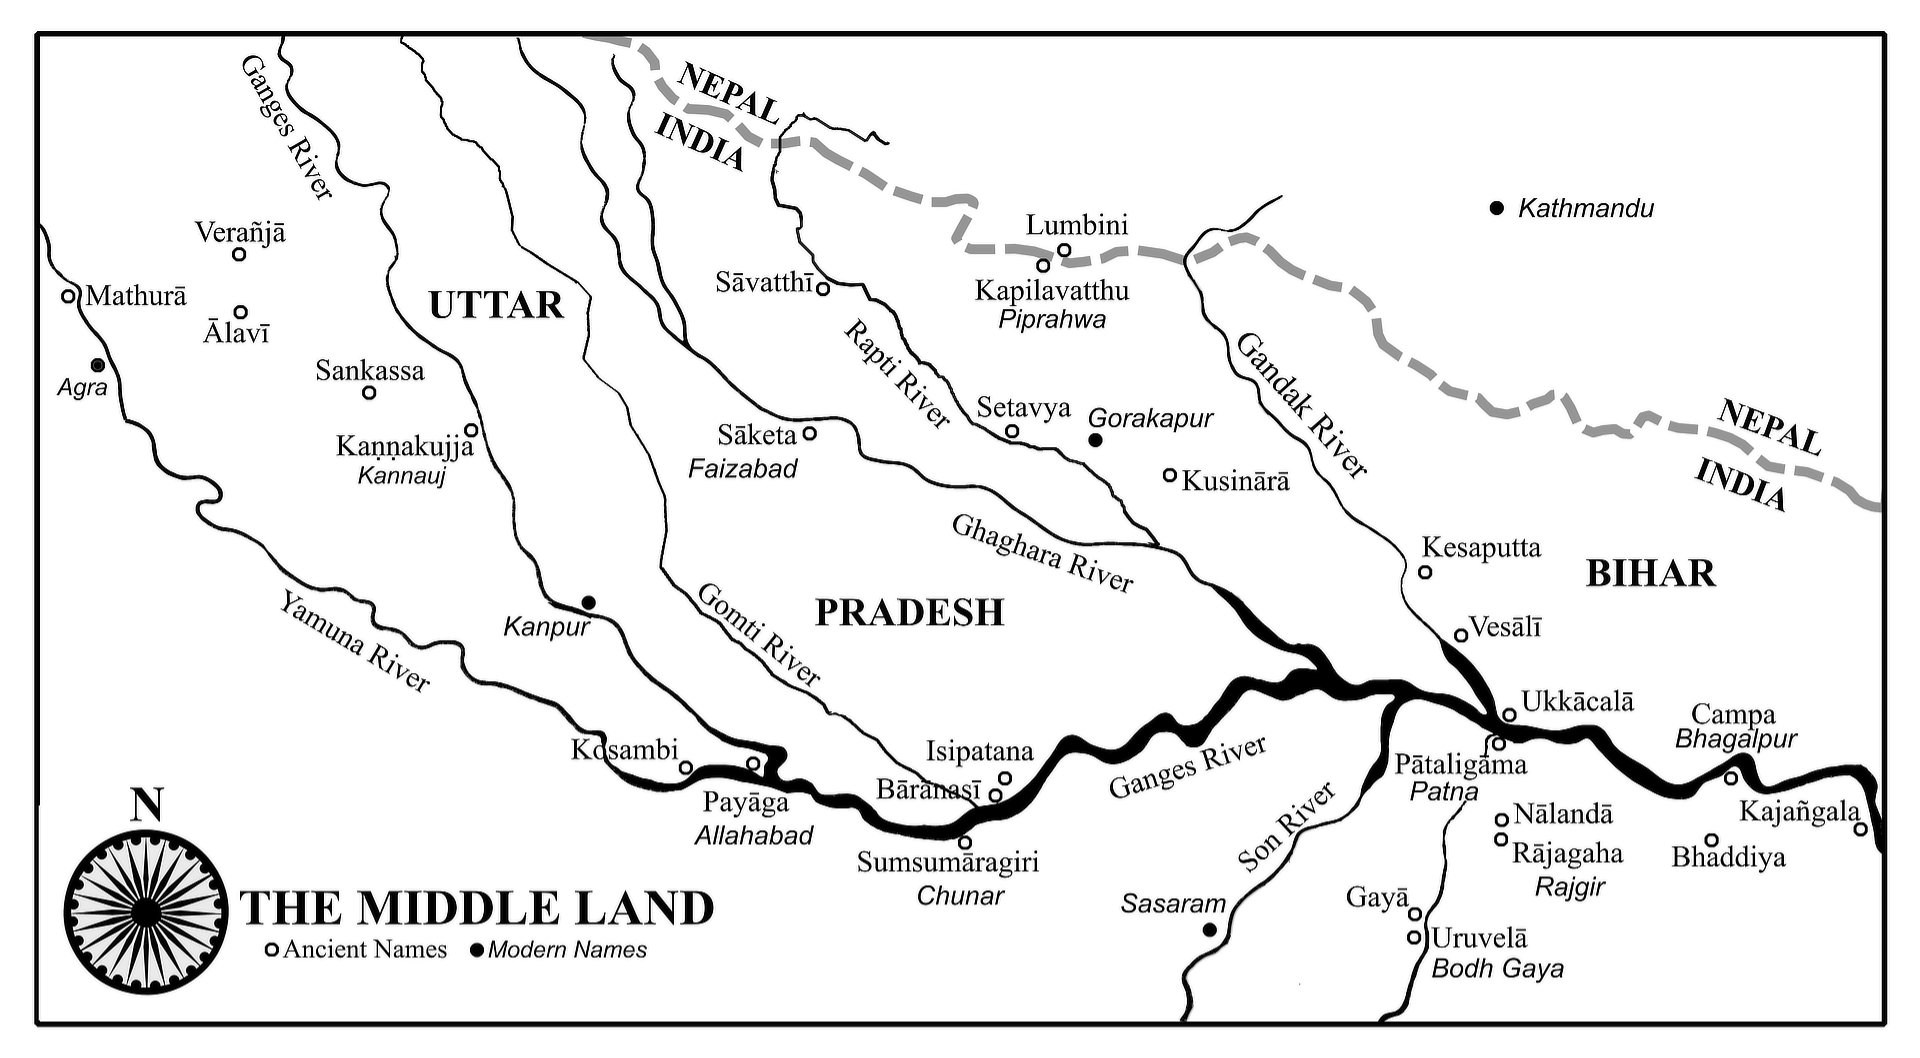
\includegraphics{middle-land-map-updated-130323-web.jpg}

As continental trade in the sixth and fifth centuries BCE grew, so did
the network of roads throughout the Middle Land. Their quality improved
too. What had been little more than footpaths and jungle tracks
gradually became proper thoroughfares. Strong centralized governments
such as those of Magadha, Kosala and Vaṃsā played a part in this
transformation too. Governments had a stake in encouraging trade because
custom charges and tolls for the use of roads and ferries helped to fill
their coffers, and troops could be dispatched quickly to troublesome
outer provinces or engage invaders. Tolls for ferries and at fords were
standardized, while wandering ascetics, brahmins and pregnant women were
generally allowed to pass
free.\phantomsection\label{footprints_split_012.html_fnref404}\hyperref[footprints_split_024.htmlux5cux23fn404]{\textsuperscript{404}}
Religion played a minor part in this transformation too. Pilgrimage was
already drawing the faithful to holy sites, and the Buddha observed that
people would go to bathe in sacred rivers such as the Sundarikā,
Sarassatī and Bahumatī and at places such as Gayā, Payāga and elsewhere.
The Buddha himself encouraged his disciples to visit at least once the
places where the seminal events in his life occurred: where he was born;
awakened; proclaimed the Dhamma for the first time; and where he would
pass
away.\phantomsection\label{footprints_split_012.html_fnref405}\hyperref[footprints_split_024.htmlux5cux23fn405]{\textsuperscript{405}}

The Tipitaka mentions a variety of thoroughfares: footpaths; jungle
tracks; lanes; and high roads, such as the ones that ran between
Sāvatthī and Verañjā, Sāvatthī and
Sāketa,\phantomsection\label{footprints_split_012.html_fnref406}\hyperref[footprints_split_024.htmlux5cux23fn406]{\textsuperscript{406}}
and the one that came from Ukkalā and passed through Uruvelā. There were
also what were called chariot roads, which were probably fairly well
maintained to facilitate the passage of such
vehicles.\phantomsection\label{footprints_split_012.html_fnref407}\hyperref[footprints_split_024.htmlux5cux23fn407]{\textsuperscript{407}}
However, it is almost certain that even the best thoroughfares were
dusty, rutted, maintained only intermittently, and perhaps impassable
during the rainy season. The Buddha mentioned how a carter on a
smooth-surfaced highway might take a shortcut and end up with a broken
axle because of the byway's uneven
surface.\phantomsection\label{footprints_split_012.html_fnref408}\hyperref[footprints_split_025.htmlux5cux23fn408]{\textsuperscript{408}}
The Jātaka tells of a civic-minded villager who mobilised his friends to
help remove large stones from roads, fell roadside trees that might hit
passing vehicles and break their axles, construct bridges, watering
places and rest houses for the convenience of travellers. Such stories
must reflect things that people actually did and encouraged others to
follow their example, thereby easing the difficulties of the being on
the
road.\phantomsection\label{footprints_split_012.html_fnref409}\hyperref[footprints_split_025.htmlux5cux23fn409]{\textsuperscript{409}}

The numerous rivers that run through the Middle Land were a hindrance to
communication. Bridges were rare, and although there were ferries on
some main arteries, fords were the main way of crossing rivers. In
places where such conveniences were unavailable, travellers would have
to improvise. The Tipitaka recounts how monks arrived at a river just as
a cowherd was driving his cattle into the water, so they clung to the
animals' tails and backs and were carried across by
them.\phantomsection\label{footprints_split_012.html_fnref410}\hyperref[footprints_split_025.htmlux5cux23fn410]{\textsuperscript{410}}
Rivers in more remote areas could be crossed by improvising a raft or
float from nearby tree branches, foliage and grass. An alternative to
getting to one's destination overland was to go by boat. The Tipitaka
mentions Ānanda embarking on a boat, probably at Pāṭaligāma, and sailing
up the Ganges to Kosambī, one of the few references to long distance
riverine travel in the
Tipitaka.\phantomsection\label{footprints_split_012.html_fnref411}\hyperref[footprints_split_025.htmlux5cux23fn411]{\textsuperscript{411}}
Many roads ran through inhabited areas with villages and their
cultivated fields, but just as many passed through jungle or semi-desert
wilderness. One traveller commented: ``These wilderness roads have
little water and food, and it is not easy to go along them without
taking provisions for the
journey.''\phantomsection\label{footprints_split_012.html_fnref412}\hyperref[footprints_split_025.htmlux5cux23fn412]{\textsuperscript{412}}
During the summer, even relatively short stretches of road posed a
threat if water was unavailable, and thus monks would carry water pots
(\emph{karaka}) and water strainers (\emph{parissāvana}) when going on
long journeys.

Beyond this, the perennial problem of travel in India has always been
banditry. The Buddha described some roads as ``frightening, dangerous
and along which one must go with a weapon'' because of the chance of
being robbed, or worse, and how travellers carrying valuables through a
wilderness area would experience relief when emerging safely from
it.\phantomsection\label{footprints_split_012.html_fnref413}\hyperref[footprints_split_025.htmlux5cux23fn413]{\textsuperscript{413}}
Travellers on the road between Sāvatthī and Sāketa were often robbed,
and at one time a fearsome robber dubbed Aṅgulimāla, who murdered his
victims, operated in forested areas in
Kosala.\phantomsection\label{footprints_split_012.html_fnref414}\hyperref[footprints_split_025.htmlux5cux23fn414]{\textsuperscript{414}}
The Buddha observed that such highwaymen would strike from and then
disappear back into ``impenetrable grass or trees, a gully or a great
forest.''\phantomsection\label{footprints_split_012.html_fnref415}\hyperref[footprints_split_025.htmlux5cux23fn415]{\textsuperscript{415}}
Some of these men would capture a party of travellers and release one of
them to go and try to get a ransom for the
others.\phantomsection\label{footprints_split_012.html_fnref416}\hyperref[footprints_split_025.htmlux5cux23fn416]{\textsuperscript{416}}
Once, the Buddha and his attendant Nāgasamāla were travelling through
Kosala when they came to a fork in the road. The Buddha said they should
take one fork, while the attendant insisted on the other. This
disagreement continued for some time until, in a huff, the attendant put
the Buddha's bowl down and walked off on the way he thought correct. He
hadn't gone far when he was attacked by bandits, who punched and kicked
him and tore his
robe.\phantomsection\label{footprints_split_012.html_fnref417}\hyperref[footprints_split_025.htmlux5cux23fn417]{\textsuperscript{417}}

More normally, though, long distance travel was just uncomfortable,
tedious and undertaken only when necessary. And yet despite these and
other problems, the Buddha spent much of his time on the road in order
to reach as many people as possible -- such was his determination and
compassion. In keeping with the rules laid down by himself and in
accordance with a long established samaṇa tradition, he would spend the
three months of the rainy season in one location and the rest of the
year on what were called walking tours. According to a quite plausible
later tradition, after the twenty-fifth year of his ministry the Buddha
spent every rainy season except the last one in or around Sāvatthī,
which would explain why more of his discourses are set in that city than
in any other
place.\phantomsection\label{footprints_split_012.html_fnref418}\hyperref[footprints_split_025.htmlux5cux23fn418]{\textsuperscript{418}}
If true, he may have decided to limit his wanderings to the region
around Sāvatthī at that time due to age, as he would have been about
sixty; because the Kosalan language was the same or similar to his own;
and perhaps because the city was only a four or five-day walk from his
hometown.

After his awakening, the Buddha set out on a long journey to find his
five former companions and share his discovery with them. Equally
significant was that his instruction to them and his next group of
disciples was that they should wander through the countryside teaching
others what he had taught them ``for the welfare of the
many.''\phantomsection\label{footprints_split_012.html_fnref419}\hyperref[footprints_split_025.htmlux5cux23fn419]{\textsuperscript{419}}
The Buddha warned his monks and nuns against prolonged aimless wandering
but also staying for too long in one place. The first would deprive them
of time with learned monastics and of forming fruitful friendships with
others, while the second could lead to accumulating too many things, of
getting involved with lay people and all their problems, or becoming too
attached to a particular
location.\phantomsection\label{footprints_split_012.html_fnref420}\hyperref[footprints_split_025.htmlux5cux23fn420]{\textsuperscript{420}}

It is possible to get at least some idea about the extent of the area
the Buddha travelled through during his teaching career. His movements
northward were limited by what were then the trackless forests of the
Himalayan foothills, although there is a single reference to him once
staying in a forest hut in a part of these hills controlled by
Kosala.\phantomsection\label{footprints_split_012.html_fnref421}\hyperref[footprints_split_025.htmlux5cux23fn421]{\textsuperscript{421}}
There is no evidence that he ever went into the mountains of the
southern edge of the Ganges Yamuna plain -- the Mizrapur Hills, the
Rajmahal Hills and the Vindhyachal Range -- or even approached them. The
furthest east he ever went that can still be identified was Kajaṅgala
and the furthest west was Madhurā. This first place corresponds to the
modern towns of Kankjol in Rajmahal District, Jharkhand, and Mathurā is
the modern Madhura, a hundred and fifty kilometres south of Delhi.
Kankjol and Mathura are nearly a thousand kilometres from each other as
the crow flies. It is uncertain how thoroughly the Buddha covered this
area, but during fifty years of wayfaring, he could have easily
travelled through much of it. The Tipitaka names over nine hundred
places that he visited or passed through: cities; towns; villages;
hills; caves; rivers; forests; and other landmarks. Thus, he may well
have wandered over an area of at least 280,000 square kilometres,
although a good deal of this would have taken place in the eastern part
of this area, between the great cities of Sāvatthī, Rājagaha, Vesālī and
Kosambī.

The Tipitaka records the itinerary of several of the Buddha's journeys,
giving some idea of the distances he sometimes travelled. For example,
we know that, within the first twelve months of his awakening, he went
from Uruvelā to Isipatana via Gayā and Bārāṇasī, spent the three months
of the rainy season there, and then made his way from there back to Gayā
and then on to Lativana and Rājagaha. All these places can be identified
with certainty, and thus it can be calculated that the Buddha walked at
least 300 kilometres from Uruvelā to Rājagaha. During another tour he
went from Verañja to Bārāṇasī via Soreyya, Saṅkassa and Kaṇṇakujja,
crossing the Ganges at Payāga. Although not explicitly mentioned in the
text, he probably took a boat down the Ganges from Payāga to
Bārāṇasī.\phantomsection\label{footprints_split_012.html_fnref422}\hyperref[footprints_split_025.htmlux5cux23fn422]{\textsuperscript{422}}
Verañjā is the modern Atranji Khera near Etah, Kaṇṇakujja is the modern
Kannauj, both of them in Uttar Pradesh, and ancient Payāga is identified
with Jhusi across the river from modern
Allahabad.\phantomsection\label{footprints_split_012.html_fnref423}\hyperref[footprints_split_025.htmlux5cux23fn423]{\textsuperscript{423}}
This tour would have involved walking at least six hundred kilometres.
In the longest single journey recorded in the Tipitaka, the Buddha went
from Rājagaha to Vesālī to Sāvatthī and back to Rājagaha via Kīṭāgiri
and Ālavī, the modern town of Airwa, a round trip of about 1,600
kilometres.\phantomsection\label{footprints_split_012.html_fnref424}\hyperref[footprints_split_025.htmlux5cux23fn424]{\textsuperscript{424}}
It is likely that he would have started a trip like this at the end of
the rainy season and arrived back in time for the next one nine months
later.

How much time the Buddha's journeys might have taken can only be guessed
at, although the ancient commentary mentions that a journey he made from
Rājagaha to Kapilavatthu took him two months, walking at one yojana a
day. From the Mahāparinibbāna Sutta we know that he went from Rājagaha
to Kusinārā via Nāḷandā, Pāṭaligāma (modern Patna), and Vesālī, a total
distance of about three hundred kilometres. According to this text, he
left Vesālī after the end of the rainy season (mid October) and died in
Kusinārā, according to tradition, on the full moon of Vesākha
(May/June). If he left Vesālī shortly after the end of the rainy season,
it would mean it took seven months for the Buddha to travel about
ninety-five kilometres, which seems like a very long time, even allowing
for the fact that he was old and in ill health. However, at some time
before leaving Vesālī, he predicted that he only had three more months
to live, meaning that he would have passed away in
January.\phantomsection\label{footprints_split_012.html_fnref425}\hyperref[footprints_split_025.htmlux5cux23fn425]{\textsuperscript{425}}
But it should be pointed out that we do not know when he left Vesālī -
it could have been weeks or even a month or two after the end of the
rainy season - and also that nowhere in the Tipitaka does it explicitly
say that the Buddha died at
Vesākhā.\phantomsection\label{footprints_split_012.html_fnref426}\hyperref[footprints_split_025.htmlux5cux23fn426]{\textsuperscript{426}}

It can be conjectured that, when the Buddha was on a walking tour, he
would wake before sunrise and go for alms gathering to the nearest
available place: a village, town or the city he was staying near. After
eating his meal, he would set off while it was still cool. He might walk
until the midday heat became unpleasant and then take an afternoon rest,
or if a village on the way seemed a good place to stop and talk with the
locals, he might stay there for the rest of the day or for two or three
days. If he arrived at a town or village later in the afternoon, he
would probably stay there until the following morning.

There are records of the Buddha sleeping in a roadside rest house, a
chaff hut, a brahmin's fire hall, an old potter's shed and, when nothing
else was available, in the open under a grove of
trees.\phantomsection\label{footprints_split_012.html_fnref427}\hyperref[footprints_split_025.htmlux5cux23fn427]{\textsuperscript{427}}
On one of his return visits to Kapilavatthu, he could find no
accommodation and had to make do in the simple hermitage of the ascetic
Bharaṇḍu; and once, when he was in the Kuru country, he stayed in a
small hut carpeted with
grass.\phantomsection\label{footprints_split_012.html_fnref428}\hyperref[footprints_split_025.htmlux5cux23fn428]{\textsuperscript{428}}
When convenient, the Buddha would lodge at religious shrines or local
sacred trees. These places often had some kind of shelter next to them
which were the scene of occasional large gatherings. Others may have had
nothing more than small huts adjacent -- basic, but convenient for a few
nights' stay.

Another option was to stay in one of the rest houses that governments,
guilds or pious individuals built along some roads or in towns for the
benefit of travellers. Many cities had such buildings just outside their
main gates so that travellers who arrived at night after the gates were
closed would have somewhere to
stay.\phantomsection\label{footprints_split_012.html_fnref429}\hyperref[footprints_split_025.htmlux5cux23fn429]{\textsuperscript{429}}
There were also royal rest houses for the use of the king or government
officials travelling on state
business.\phantomsection\label{footprints_split_012.html_fnref430}\hyperref[footprints_split_025.htmlux5cux23fn430]{\textsuperscript{430}}
Most public travellers' rests provided shelter and little else, although
in the town of Uttara, for example, the headman Pāṭaliya built and
maintained one that had basic but adequate furniture and
fittings.\phantomsection\label{footprints_split_012.html_fnref431}\hyperref[footprints_split_025.htmlux5cux23fn431]{\textsuperscript{431}}
A few provided food for anyone who might turn up. Once, a group of monks
went to a rest house for alms so often that the locals grumbled, saying:
``The alms food is not prepared just for them; it's supposed to be for
everyone.'' Anxious that his monks not get a reputation for greed, the
Buddha made it a rule that monks should go for alms at such places no
more than once, unless they were
sick.\phantomsection\label{footprints_split_012.html_fnref432}\hyperref[footprints_split_025.htmlux5cux23fn432]{\textsuperscript{432}}
He also made it a rule that monks should not use an umbrella or a
walking staff when travelling. In the case of umbrellas, this was
because they were associated with power and status, and he did not want
people to think his monks were putting on airs. A group of monks using
umbrellas was mocked for looking like treasury officials
(\emph{gaṇakamahāmatta}).\phantomsection\label{footprints_split_012.html_fnref433}\hyperref[footprints_split_025.htmlux5cux23fn433]{\textsuperscript{433}}
Monks and nuns were allowed to use sandals, although there is no record
of the Buddha having a pair or using them.

How long the Buddha stayed at a particular place would have depended on
many factors: whether local people came to talk with and listen to him;
whether alms and water were available; and whether the atmosphere was
congenial. When staying in large population centres, his accommodation
would have been reasonably comfortable, and he would have been
well-provided for. When he returned to Rājagaha after his awakening,
King Bimbisāra donated one of his pleasure parks, the Bamboo Grove, to
the Saṅgha, a gift followed by many others in the coming decades. The
first monasteries established on such properties were little more than
small thatched wattle and daub huts or shelters made of leaves, foliage
or grass. Only later in the Buddha's career were more permanent
structures built. The Jetavana, the first large, purpose-built monastic
complex, had halls, covered walkways, wells, bathrooms and other
amenities.\phantomsection\label{footprints_split_012.html_fnref434}\hyperref[footprints_split_025.htmlux5cux23fn434]{\textsuperscript{434}}
This monastery flourished right up to Indian Buddhism's last days in the
twelfth century.

The Buddha must have enjoyed the freedom his life of wandering gave him.
He said: ``The household life is full of hindrances, a path of dust.
Free as the breeze is the life of one who renounces all worldly
things.''\phantomsection\label{footprints_split_012.html_fnref435}\hyperref[footprints_split_025.htmlux5cux23fn435]{\textsuperscript{435}}
Moving from place to place allowed him to spread his teachings, but
there were other reasons behind it too. He was aware that some personal
contact with him was important for his disciples, especially for newly
ordained monks and nuns, and this was sometimes a factor in determining
which districts he visited and how
often.\phantomsection\label{footprints_split_012.html_fnref436}\hyperref[footprints_split_025.htmlux5cux23fn436]{\textsuperscript{436}}
During his wanderings he might visit a district, teach, make some
disciples, even ordain a few monks or nuns, and then perhaps not come
again for years. For lay disciples with domestic obligations,
undertaking a long journey to see the Buddha would have been difficult,
and so they had to wait, perhaps years, before they got to see him
again. One text gives us some idea of the excitement caused in an
outlying district when its inhabitants heard that the Buddha might be on
his way to their village and how the excitement increased as word of his
gradual approach reached
them.\phantomsection\label{footprints_split_012.html_fnref437}\hyperref[footprints_split_025.htmlux5cux23fn437]{\textsuperscript{437}}
Once, a monk who had spent the rainy season with the Buddha in Sāvatthī
arrived in Kapilavatthu. When people heard where he had come from, he
found himself deluged with questions about the Buddha and what he had
been
teaching.\phantomsection\label{footprints_split_012.html_fnref438}\hyperref[footprints_split_025.htmlux5cux23fn438]{\textsuperscript{438}}

Naturally, the Buddha could not be everywhere at once, and so monks and
nuns would sometimes have to undertake long journeys for the privilege
of spending time in his presence. For example, while he was residing in
Catuma, a few hundred monks arrived in the city to be with him and
listen to
him.\phantomsection\label{footprints_split_012.html_fnref439}\hyperref[footprints_split_025.htmlux5cux23fn439]{\textsuperscript{439}}
Another example concerns the monk Sona Kutikaṇṇa who ordained under the
tutorage of Mahā Kaccāna. About a year later, he developed the desire to
meet the man whose teachings he had committed himself to. He said to his
preceptor: ``I have not yet met the Lord face to face; I have only heard
about what he is like. If you give me permission, I will travel to see
the Lord, the Worthy One, the fully awakened
Buddha.''\phantomsection\label{footprints_split_012.html_fnref440}\hyperref[footprints_split_025.htmlux5cux23fn440]{\textsuperscript{440}}
He was able to fulfil this wish.

Those wanting to know where the Buddha was in order to meet him could
find they had a problem if they came from a distant region or another
country. But an official in the court of King Pasenadi, who was an
admirer of the Buddha, was sometimes able to know his whereabouts at any
given time or where he was travelling from or to because of the
information he received, presumably from monks, merchants or his fellow
royal officers who had come from outlying districts or even other
countries.\phantomsection\label{footprints_split_012.html_fnref441}\hyperref[footprints_split_025.htmlux5cux23fn441]{\textsuperscript{441}}

There are three examples of people coming from beyond the Middle Land to
meet the Buddha, evidence that his reputation had spread to adjacent
regions of India. There is an account of the sixteen disciples of the
ascetic Bāvari setting out from the Godavari, probably from where it
flows through Maharashtra, for the Middle Land in the hope of meeting
the Buddha. When they heard that he was at Sāvatthī, they headed there,
going through Kosambī and Sāketa, and arrived in Sāvatthī only to learn
that he had left some time previously. They followed his route through
Setavya, Kapilavatthu, Kusinārā, Pāvā and Vesālī, finally catching up
with him at the Pasanaka
Shrine.\phantomsection\label{footprints_split_012.html_fnref442}\hyperref[footprints_split_025.htmlux5cux23fn442]{\textsuperscript{442}}
The ascetic known as Bark Blanket Bāhiya is said to have come all the
way from Suppāraka to meet the
Buddha.\phantomsection\label{footprints_split_012.html_fnref443}\hyperref[footprints_split_025.htmlux5cux23fn443]{\textsuperscript{443}}
This place, now called Sopara, is on the west coast of India some
fifty-five kilometres north of Mumbai. That the Buddha's reputation
could have reached so far and that Bāhiya could have travelled such a
distance, some 1300 kilometres, is not as far-fetched as it might first
seem. Suppāraka was a major seaport and the terminus of the
Dakkhinapātha, the great highway that started at Kosambī, and was
already a major emporium by the fifth century BCE. Merchants may well
have brought news of the Buddha to Suppāraka, and Bāhiya may well have
travelled to the Middle Land with a merchant caravan headed
there.\phantomsection\label{footprints_split_012.html_fnref444}\hyperref[footprints_split_025.htmlux5cux23fn444]{\textsuperscript{444}}
Another story tells of the monk Soṇa, who came all the way from the
kingdom of Avanti to meet the Buddha. Avanti was a kingdom to the south
of the Middle Land, linked to it by the
Dakkhiṇāpatha.\phantomsection\label{footprints_split_012.html_fnref445}\hyperref[footprints_split_025.htmlux5cux23fn445]{\textsuperscript{445}}
These stories indicate just how mobile the ascetics of the time could
be.

There would have been as many languages and dialects spoken in the
Middle Land as there are in that region today, and this would have
created special problems for someone like the Buddha, who travelled
widely. Theravāda tradition maintains that the Buddha spoke Pali,
although there is no mention in the Tipitaka of what his mother tongue
was. As with merchants, diplomats and others whose professions required
frequent long distance travel in different regions, he may well have
been competent in several languages. The Buddha said that insisting on
using one's own language or dialect in an area where another is spoken
can only cause confusion and discord:

\begin{quote}
``It has been said, `One should not stake too much on the local
language\ldots' How does one do this? In different regions they might
call the same thing a bowl, basin, dish, crock, vessel, tureen, concave
container or rounded receptacle. But whatever they call it in one
region, one uses that word, thinking, `It seems this person is referring
to that object', and one uses that word
accordingly.''\phantomsection\label{footprints_split_012.html_fnref446}\hyperref[footprints_split_025.htmlux5cux23fn446]{\textsuperscript{446}}
\end{quote}

Nor did he believe that any one language communicated his Dhamma any
better than any other, saying: ``I want you to learn the Buddha's words
each in your own
language.''\phantomsection\label{footprints_split_012.html_fnref447}\hyperref[footprints_split_025.htmlux5cux23fn447]{\textsuperscript{447}}
The Buddha was equally open about regional customs. On one occasion he
said:

\begin{quote}
``I clearly remember all the assemblies of nobles, brahmins,
householders, ascetics and gods\ldots I have attended. Before I sat with
them, spoke with them or joined their conversations, I adopted their
expression, their speech, whatever it might be, and then I instructed
them in
Dhamma.''\phantomsection\label{footprints_split_012.html_fnref448}\hyperref[footprints_split_025.htmlux5cux23fn448]{\textsuperscript{448}}
\end{quote}

This is the kind of thing one would expect of an urbane, open-minded and
well-travelled individual. Whatever the Buddha was, he was not
parochial, and no doubt his travels made him even more flexible and
tolerant of differences.

\phantomsection\label{footprints_split_012.html_calibre_pb_25}

\phantomsection\label{footprints_split_013.html}{}

\section{\texorpdfstring{{Chapter 9}\\
Praise and
Blame}{Chapter 9 Praise and Blame}}\label{footprints_split_013.html_TOCTarget9}

There was not, there is not now,\\
and there never will be someone\\
who is wholly blamed or praised.

Dhammapada 228\\
\href{https://suttacentral.net/dhp228/en/sujato}{Dhp\,228}

Having been in the public arena for so long and proclaiming ideas that
challenged many of the existing ones, the Buddha of course attracted
opposition, criticism and sometimes even antipathy. When this happened
he would attempt to justify his position by explaining himself more
fully, while remaining unruffled and not striking back at his critics.
Likewise, he instructed his disciples not to be provoked but remain as
objective as possible when he, they, or the teaching were targets of
criticism or misrepresentation or even when any of the three were
praised:

\begin{quote}
``If anyone should criticise me, the Dhamma or the Saṅgha, you should
not because of that be angry, resentful or upset. For if you did, that
would hinder you and you would not be able to know whether what they
said was right or wrong. Would you?''

``No, Lord.''

``Therefore, if others criticise me, the Dhamma or the Saṅgha, simply
explain what is incorrect, saying, `That is incorrect. That is not
right. That is not our way. We do not do that.' Likewise, if others
should praise me, the Dhamma or the Saṅgha, you should not because of
that be pleased, elated or self-satisfied. For if you were, that would
hinder you. Therefore, if others praise me, the Dhamma or the Saṅgha,
then simply explain what is correct, saying: `That is correct. That is
right. That is our way. That is what we
do.'\,''\phantomsection\label{footprints_split_013.html_fnref449}\hyperref[footprints_split_025.htmlux5cux23fn449]{\textsuperscript{449}}
\end{quote}

Within a year of the Buddha's awakening, he had made disciples of his
five former companions, the wealthy young man Yasa and his friends, and
the three Kassapa brothers who were the most well-known and esteemed
samaṇas in Magadha, together with all their followers. Shortly after
this, most of the followers of another samaṇa teacher, Sañjaya
Belaṭṭhiputta, some two hundred and fifty in all, abandoned him to join
the Buddha's Saṅgha also. These last two events created great interest
throughout Magadha and made the Buddha well-known early in his career.
Soon, numerous young men were requesting to become monks, and the Buddha
was happy to accept them all. But his readiness to ordain anyone who
asked for it created problems. Ill-trained and unsupervised monks were
soon wandering all over the place causing embarrassment. Also, with many
youths and men abandoning their families, this created disquiet amongst
the people affected by it and led to grumbling against the Buddha
himself. People were saying: ``The samaṇa Gotama proceeds by making us
childless, by making us widows, by breaking up families.'' If the Buddha
was concerned by this, he did not mention it. When informed of what
people were saying about him, he dismissed it, commenting: ``This noise
will not last long; it will continue for seven days and then
cease.''\phantomsection\label{footprints_split_013.html_fnref450}\hyperref[footprints_split_025.htmlux5cux23fn450]{\textsuperscript{450}}
Only after this did he start laying down rules for vetting candidates
and for ordaining and training monks. He had apparently not given
sufficient thought to the proper organisation of his order before
accepting large numbers of men into it.

Although the Buddha saw himself firmly within the non-Vedic samaṇa
tradition, he disregarded some of its most basic assumptions,
particularly the practice of rigorous austerities (\emph{tapa}) and
self-mortification (\emph{attakilamatha}). For this he was sometimes
criticised by other ascetics. When, after for or five years of
undergoing such disciplines himself, he finally abandoned them and
started washing and eating properly again, the five disciples who had
attached themselves to him were outraged. They accused him of reverting
to the life of abundance (\emph{āvatto bahullāya}) and left him in
disgust. One ascetic dismissed him as a ``shaven-headed householder''
(\emph{muṇḍagahapatika}) meaning that he was little more than a layman
posing as an
ascetic.\phantomsection\label{footprints_split_013.html_fnref451}\hyperref[footprints_split_025.htmlux5cux23fn451]{\textsuperscript{451}}
The ascetic Kassapa repeated to the Buddha an accusation he had heard
about him: ``The samaṇa Gotama disapproves of all austerities; he
criticises and blames all those who live the hard life.'' The Buddha
denied this, explaining that he praised austerities that led to
understanding and liberation and criticised those that did
not.\phantomsection\label{footprints_split_013.html_fnref452}\hyperref[footprints_split_025.htmlux5cux23fn452]{\textsuperscript{452}}
As will be shown below, it is probable that the real reason for
Devadatta breaking with the Buddha and founding his own Saṅgha was the
Buddha's de-emphasis of the value of austerity and self-mortification.

A few of the more extreme ascetics accused the Buddha of being careless
with life. When the ascetic Māgandiya saw the grass spread out on the
floor where the Buddha was sleeping, he commented: ``It is a sorry sight
indeed when we see the bed of samaṇa Gotama, that destroyer of
growth.''\phantomsection\label{footprints_split_013.html_fnref453}\hyperref[footprints_split_025.htmlux5cux23fn453]{\textsuperscript{453}}
It is not entirely certain what this criticism meant, but it is likely
that Māgandiya accepted the belief, current at the time amongst certain
samaṇas, that plants were sentient life, and thus to pluck or cut them
was tantamount to killing, something the more scrupulous ascetic
avoided. Some ascetics went so far as to carry brooms or whisks to sweep
the ground before them as they walked to avoid treading on and killing
tiny
insects.\phantomsection\label{footprints_split_013.html_fnref454}\hyperref[footprints_split_025.htmlux5cux23fn454]{\textsuperscript{454}}
Given such scrupulousness, it is hardly surprising that the Jains, who
were strict vegetarians, attacked the Buddha and his disciples for
eating meat.

\begin{quote}
``A crowd of Jains went through the town, from street to street, from
one square to another, waving their arms and shouting, `The general Sīha
has this very day slaughtered a large creature to feed to the samaṇa
Gotama, and he is going to eat it knowing that it was slaughtered
specifically for
him.'\,''\phantomsection\label{footprints_split_013.html_fnref455}\hyperref[footprints_split_025.htmlux5cux23fn455]{\textsuperscript{455}}
\end{quote}

The Buddha did not respond to the charge that accepting from a donor and
then eating a meal containing meat amounted to killing. However, he made
a rule that his monks and nuns should not accept such a meal if they
saw, heard or suspected that the meat was from an animal that had been
slaughtered specifically for
them.\phantomsection\label{footprints_split_013.html_fnref456}\hyperref[footprints_split_025.htmlux5cux23fn456]{\textsuperscript{456}}

One interesting misgiving that some people had of the Buddha was that,
despite his relative youth, he claimed to be fully awakened, while most
others making such a claim were generally old. King Pasenadi asked the
Buddha about this:

\begin{quote}
``Even those samaṇas and brahmins who are the head of orders and sects,
well-known teachers, famous and considered so by the general public --
even they do not claim to have attained the unsurpassed perfect
awakening. Therefore, how can you make such a claim when you are still
so young and have so recently become a samaṇa?''
\end{quote}

The Buddha replied that awakening had nothing to do with age, just as a
young king, a newly hatched snake or a recently ignited fire could still
have an impact and therefore should be taken
seriously.\phantomsection\label{footprints_split_013.html_fnref457}\hyperref[footprints_split_025.htmlux5cux23fn457]{\textsuperscript{457}}

As was shown previously, public discussions and debates on religious
questions were a feature of Indian society during the Buddha's time. For
some, such events were a chance to learn about the new ideas being
aired, while for a few they were an opportunity to promote themselves as
clever and entertaining disputants. There were ``certain learned nobles
who are clever, well-versed in the doctrines of others, real
hair-splitters, who go about demolishing the views of others with their
sharp intelligence. When they hear that the samaṇa Gotama will visit a
certain village or town, they formulate a question, thinking, `We will
go and ask him this question, and if he answers like this, we will say
that, and if he answers like that, we will say this and thereby refute
his Dhamma.' But when they confront the samaṇa Gotama, he instructed,
inspired, motivated and gladdened them with talk on Dharma, and they do
not so much as ask their question, let alone refute his
Dhamma.''\phantomsection\label{footprints_split_013.html_fnref458}\hyperref[footprints_split_025.htmlux5cux23fn458]{\textsuperscript{458}}
As a result of the Buddha's ability to disarm and impress such opponents
and disputants, some people suspected him of using magical power to do
so.\phantomsection\label{footprints_split_013.html_fnref459}\hyperref[footprints_split_025.htmlux5cux23fn459]{\textsuperscript{459}}

A village headman once asked the Buddha if it were true that he used
some kind of magic to convert people, and he admitted that he did, much
to the headman's surprise. ``Then it is true: the samaṇa Gotama is a
magician!'' But the Buddha then pointed out that knowing magic does not
necessarily mean being a magician
(\emph{māyākāra}).\phantomsection\label{footprints_split_013.html_fnref460}\hyperref[footprints_split_025.htmlux5cux23fn460]{\textsuperscript{460}}
What he meant becomes clear from another dialogue with someone who also
broached the subject of magic with him. Bhaddiya asked him if it were
true that he knew magic and used it to convert the disciples of other
teachers. The Buddha replied firstly by saying that one should not be
guided by, amongst other things, supposed revelations, tradition,
hearsay, the authority of the scriptures, or what a particular teacher
might claim, and he then explained aspects of his teachings in detail.
By the time he had finished, Bhaddiya was so taken by what the Buddha
had said that he asked to become a disciple. The Buddha responded:

\begin{quote}
``Now Bhaddiya, did I say to you, `Become my disciple, and I will be
your teacher'?''

``No sir.''

``Although I declare and proclaim my teaching in the manner I just gave
to you, some samaṇas and brahmins dishonestly and falsely, unfairly and
inaccurately misrepresent me by saying that I use magic to lure away the
disciples of other teachers.''

``An excellent and wonderful thing is this magic of yours! If only my
beloved kin and the members of my family could be converted by this
magic, it would be for their welfare and happiness for a long
time.''\phantomsection\label{footprints_split_013.html_fnref461}\hyperref[footprints_split_025.htmlux5cux23fn461]{\textsuperscript{461}}
\end{quote}

Another criticism of the Buddha, and, interestingly, one that continues
to be made even today, was that his concept of Nirvana and his doctrine
of not-self (\emph{anatta}) amounted to a form of nihilism
(\emph{uccedhavāda}). When accused of teaching this, he responded:
``There is a way of speaking truthfully that one could say I teach a
doctrine of annihilation and train my disciples in it. I teach the
annihilation of greed, hatred and delusion, I teach the annihilation of
all the many evil and wrong states of
mind.''\phantomsection\label{footprints_split_013.html_fnref462}\hyperref[footprints_split_025.htmlux5cux23fn462]{\textsuperscript{462}}

At the end of a discussion with the Buddha, an interlocutor would often
express his or her satisfaction with what the Buddha had said, but not
always. While on a visit to Kapilavatthu, the Buddha met his mother's
brother Daṇḍapāni, who asked him to explain his Dhamma. After listening
without comment until the Buddha had finished, the old man ``shook his
head, wagged his tongue, raised his eyebrows so that three wrinkles
formed on his forehead, and then walked off, leaning on his
stick.''\phantomsection\label{footprints_split_013.html_fnref463}\hyperref[footprints_split_025.htmlux5cux23fn463]{\textsuperscript{463}}
After giving a talk to a group of his own monks at Ukkaṭṭhā, we are told
that they were far from delighted by what he had
said.\phantomsection\label{footprints_split_013.html_fnref464}\hyperref[footprints_split_025.htmlux5cux23fn464]{\textsuperscript{464}}
Once, during a talk with a brahmin, the Buddha compared brahmins who so
confidently explained what the ancient sages taught, while admitting
that they themselves did not share their attainments, to a string of
blind men. ``The first one does not see, the middle one does not see and
neither does the last.'' At this, the brahmin became extremely angry and
threatened the Buddha, saying: ``The samaṇa Gotama will be
disgraced!''\phantomsection\label{footprints_split_013.html_fnref465}\hyperref[footprints_split_025.htmlux5cux23fn465]{\textsuperscript{465}}
In this case, there was a rapproachment, the discussion continued and
eventually the brahmin developed some respect for the Buddha.

The Tipitaka also records a few examples where some of the Buddha's
disciples abandoned him. Throughout the texts, people who had been
conversing with the Buddha typically express their appreciation for what
he had said and announce that they wish to become one of his disciples
``for as long as life lasts''. While such sentiments are usually couched
in a stereotyped form, there is no reason to doubt that many people did
say something like this. However, this does not mean that they meant
what they said: some were probably just being polite, while others may
have meant what they said, but after their initial enthusiasm wore off,
they may have returned to their old beliefs or just lost interest in the
Dhamma. A few may have momentarily wanted to become a disciple but then
had second thoughts. After listening to the Buddha, the ascetic teacher
Sakuludāyin expressed the wish to become a disciple, unil his dismayed
followers pleaded with him: ``Master, don't become a monk under samaṇa
Gotama! Having been a teacher don't become a student! It would be as if
a large jug should become a small mug''. The thought of losing his
status made Sakuludāyin change his
mind.\phantomsection\label{footprints_split_013.html_fnref466}\hyperref[footprints_split_025.htmlux5cux23fn466]{\textsuperscript{466}}

A close reading of the Tipitaka reveals that there were people who had
been Buddhists, and even monks, and later left. Once, some thirty monks
being trained by Ānanda disrobed en masse, although it is not certain
whether they were dissatisfied with Ānanda's tutelage, realized that the
monastic life was not for them, or were no longer convinced about the
Dhamma.\phantomsection\label{footprints_split_013.html_fnref467}\hyperref[footprints_split_025.htmlux5cux23fn467]{\textsuperscript{467}}
On another occasion, the Buddha gave a long talk to a group of monks in
which he told them that they should use the basic requirements for life
given to them by devotees with great care and strive resolutely for
their own benefit while at the same time considering the good of others.
Some sixty of the monks became extremely angry, perhaps thinking that
the Buddha was indirectly reproaching them, and another sixty told him:
``That is difficult to do Lord, very difficult'' and then announced that
they had decided to
disrobe.\phantomsection\label{footprints_split_013.html_fnref468}\hyperref[footprints_split_025.htmlux5cux23fn468]{\textsuperscript{468}}
Sunakkhatta had once served as the Buddha's attendant. After seeing
ascetics who had taken rigorous vows, such as restricting their
movements to very small areas or practicing bizarre austerities such as
going naked and imitating the behaviour of dogs or cows, he developed an
admiration for them. Compared with such attention-grabbing practices,
the disciplines and lifestyles taught by the Buddha seemed rather tame.
Eventually, he went to the Buddha and announced: ``Sir, I am leaving
you. I am no longer living by your guidance.'' The Buddha responded to
this declaration by questioning Sunakkhatta:

\begin{quote}
``Did I ever say to you, `Come, live by my guidance?'\,''

``No sir.''

``Then did you ever say to me, `I wish to live by your guidance?'\,''

``No sir.''

``So if I never made such a promise to you and you never gave such a
condition to me, who are you to be giving up anything, you foolish
man?''

``But sir, you never performed any super-human wonders, any psychic
powers or any miracles for me.''

``Did I ever say to you, `Come, live by my guidance and I will perform
such things for you?'\,''

``No sir.''
\end{quote}

The Buddha then explained his position on miracles and psychic powers,
saying that they were one thing and overcoming suffering was another and
that he was primarily interested in this latter goal. These words did
not placate Sunakkhatta, and he left the Saṅgha. Subsequently, he let it
be widely known that he no longer had any confidence in or respect for
the Buddha.

\begin{quote}
``The samaṇa Gotama has no extraordinary powers or any special knowledge
or vision one would expect of a true worthy one. What he teaches has
been hammered out by reason and according to his own notions. When he
teaches his Dhamma to someone, it only leads them to the ending of
suffering.''
\end{quote}

When the Buddha heard what Sunakkhatta had been telling everyone, he
said of him: ``He is an angry and foolish man and speaks out of
anger.''\phantomsection\label{footprints_split_013.html_fnref469}\hyperref[footprints_split_025.htmlux5cux23fn469]{\textsuperscript{469}}

At that time, switching from one religion to another was called `going
over to the discipleship' (\emph{sāvakattaṃ upagaccheyya}) of whatever
sect or teaching one had newly adopted. When lay people decided to
become Buddhists, they would often choose to distinguish themselves by
wearing white clothes and were usually known as ``lay people dressed in
white.'' When an ascetic or monk of another sect converted to Buddhism,
they would almost always abandon the accoutrements and practices of
their former religion, ordain, and don the tawny-coloured robe distinct
to Buddhist monastics and abide by the rules of the Vinaya. But,
apparently, this was not always the case.

The wandering ascetic Sarabha identified himself as a disciple of the
Buddha while remaining within his own sect, at least outwardly. After
some time, he decided that he was no longer a Buddhist and told anyone
he met or who would listen to him that he now rejected the Dhamma
precisely because he understood it. The Buddha would not let such a
claim pass without being challenged, and he went to see Sarabha and
questioned him: ``Is it true that you have been saying that you left the
Dhamma and training of the samaṇas who are sons of the Sakyan because
you understand it?'' Sarabha was silent. The Buddha continued: ``Then
explain to me your understanding of this Dhamma and training. If you
have not learned it completely, I will complete it for you, and if you
have learned it completely, I will be happy to hear you explain it.''
Again Sarabha did not answer, but the Buddha persisted for a second and
a third time, until it was clear that the hapless Sarabha either would
not, or more likely could not, give an answer. After explaining to the
others who had witnessed this encounter why he had interrogated Sarabha
the way he did, the Buddha got up and
left.\phantomsection\label{footprints_split_013.html_fnref470}\hyperref[footprints_split_025.htmlux5cux23fn470]{\textsuperscript{470}}

Those who dropped out of the monastic Saṅgha nonetheless sometimes
maintained their commitment to the Dhamma.

\begin{quote}
``Even those who leave the monkhood and return to the lay life still
praise the Buddha, the Dhamma and the Saṅgha. It is themselves that they
blame, saying, `We were unlucky, we had scant merit, for although we
ordained in such a well-proclaimed Dhamma, we were unable to live the
perfect and pure spiritual life for our whole lives.' Having become
monastery attendants or lay disciples, they take and observe the Five
Precepts.''\phantomsection\label{footprints_split_013.html_fnref471}\hyperref[footprints_split_025.htmlux5cux23fn471]{\textsuperscript{471}}
\end{quote}

One of the most disturbing events in the whole of the Buddha's career
happened during one of his sojourns in Vesālī. He had given a talk to an
assembly of monks about a meditation called \emph{asubha bhāvanā}. This
practice involved contemplating the unpleasant aspects of the body --
the discharges that are revolting in themselves or which soon become so
without regular washing. The purpose of this practice was to encourage
detachment towards the body, to cool sexual impulses, and to act as a
counterbalance to the usual over-emphasis on physical attractiveness.
After his talk, the Buddha announced that he wanted to go into a
solitary retreat for half a month. While he was away, the monks did this
contemplation, with tragic results for some of them. The Tipitaka
recounts that some thirty monks became so repelled and disgusted with
their bodies that they committed suicide. When the Buddha returned from
his retreat and noticed some familiar faces missing, he asked where they
were and was told what had happened. The Tipitaka records that he then
gave a talk on mindfulness of breathing meditation, emphasising its
ability to evoke tranquillity and calm, but it records nothing he had to
say about this
tragedy.\phantomsection\label{footprints_split_013.html_fnref472}\hyperref[footprints_split_025.htmlux5cux23fn472]{\textsuperscript{472}}
It is also silent about comments others may have made about this event,
although one could well imagine that some people would have been as
deeply shocked by it as most would be if it happened today. It is often
claimed that the Buddha was able to read a person's mind, or at least
sense their abilities and inclinations, and present the Dhamma to them
in such a way that it would resonate specifically with them. This
incident is evidence that he could not always do this.

As mentioned previously, Brahminism during the Buddha's time was being
re-evaluated and reinterpreted as it struggled to maintain its relevance
in a rapidly changing world and tried to compete with the samaṇa
tradition. Consequently, there were brahmins who expressed an interest
in and appreciation for some of the things the Buddha was teaching, or
at least were prepared to listen to what he had to say. Others, the more
orthodox and traditional, saw him as a serious threat and never missed
an opportunity to vent their hostility towards him, his monks and his
nuns. This hostility rarely took the form of criticism of what the
Buddha was teaching but was usually expressed in terms of his supposed
inferiority and ritual impurity. On one occasion, while alms gathering,
the Buddha approached the house of a brahmin just as he was doing his
morning rituals. Seeing him coming and not wanting his presence to make
the ritual impure, the brahmin called out: ``Stop there, you shaveling,
you miserable ascetic, you
outcaste!''\phantomsection\label{footprints_split_013.html_fnref473}\hyperref[footprints_split_025.htmlux5cux23fn473]{\textsuperscript{473}}
On another occasion, when a particular brahmin found out that a member
of his clan had joined the Buddhist Saṅgha, he went to the Buddha in a
rage and insulted
him.\phantomsection\label{footprints_split_013.html_fnref474}\hyperref[footprints_split_025.htmlux5cux23fn474]{\textsuperscript{474}}
However, there are incidents indicating divided opinions amongst
brahmins about the Buddha, with some despising him and others having
regard for him and his followers -- sometimes great regard.

It seems that the brahmini Dhānañjānī was devoted to the Buddha, and
once, as she tripped and nearly fell, she exclaimed three times:
``Praise to the Lord, the Worthy One, the fully awakened Buddha!'' The
brahmin Sangārava happened to be nearby, and, hearing this, he said in
disgust: ``This Dhānañjānī should be disgraced and degraded! In the
presence of brahmins she praises that shaven-headed
samaṇa.''\phantomsection\label{footprints_split_013.html_fnref475}\hyperref[footprints_split_025.htmlux5cux23fn475]{\textsuperscript{475}}
Once, some nuns on a journey arrived in a village and, having nowhere to
stay, they approached the house of a certain brahmini and asked her if
they could stay there overnight. She asked them to wait until her
husband returned, so they went inside, spread out their mats and sat
down while they waited. The brahmin return after nightfall and, seeing
the nuns, asked his wife who the strangers were. She replied: ``They are
nuns.'' He demanded angrily: ``Throw the shaven-headed whores
out!''\phantomsection\label{footprints_split_013.html_fnref476}\hyperref[footprints_split_025.htmlux5cux23fn476]{\textsuperscript{476}}
In these two stories, at least, brahmin women are depicted as being more
accepting of Buddhists than the men were. Other stories show that
hostility could change to tolerance and even respect when personal
contact created an opportunity for the Buddha's Dhamma to be explained.

The senior monk Mahā Kaccāna happened to be staying in the forest when
some young brahmin students out collecting firewood came across his
hut.\phantomsection\label{footprints_split_013.html_fnref477}\hyperref[footprints_split_025.htmlux5cux23fn477]{\textsuperscript{477}}
Realizing that there was a Buddhist monk inside, they circled the hut,
making a great commotion, while saying loudly that the only people who
respected monks were ignorant bumpkins. Deciding not to let this
rudeness pass, Kaccāna came out and told the students that, while the
brahmins of old led pure simple lives, their successors today had
unguarded senses and a preoccupation with chanting hymns, meaningless
rituals and outward show. Unused to being spoken to like this, the
indignant youngsters marched back to their teacher, Lohicca, and told
him that a Buddhist monk had insulted the Vedas. He was very angry and
resolved to go and confront Kaccāna but thought it best to hear his
account of the incident first. When he arrived at the hut, his students
following behind, he greeted Kaccāna politely and, after the usual small
talk, asked him if he had said what his students had reported to him.
Kaccāna confirmed that he had indeed said such things. A few moments of
uneasy silence must have followed. But then, rather than scold Kaccāna
as he had intended, Lohicca asked him what he had meant by unguarded
senses. Kaccāna took the opportunity to describe the meditation practice
of being aware of sensory impingement, the value of remaining detached
from it, and the insights that would result. Lohicca was quite impressed
by this and told Kaccāna that any time he came to his house for alms, he
would be given food with every mark of respect, including from his
students.\phantomsection\label{footprints_split_013.html_fnref478}\hyperref[footprints_split_025.htmlux5cux23fn478]{\textsuperscript{478}}

Despite the criticisms and negative assessments of some, the Buddha was
the most respected teacher of his time, along with the Jain leader
Mahāvīra, who was senior to him by about a decade. Someone who had
attended a talk by the Buddha noticed that when it was finished, the
audience got up and left reluctantly, keeping their eyes on him as they
did
so.\phantomsection\label{footprints_split_013.html_fnref479}\hyperref[footprints_split_025.htmlux5cux23fn479]{\textsuperscript{479}}
This interesting observation, and several similar ones, confirm the
impression that the Buddha had great personal charisma and, for some
people at least, that it was his good looks and commanding presence that
initially attracted them to the Dhamma.

The Tipitaka provides a great deal of information about the Buddha's
physical appearance. We are told that he was four finger-breadths taller
than his handsome and younger half-brother Nanda, who could be mistaken
for him from a
distance.\phantomsection\label{footprints_split_013.html_fnref480}\hyperref[footprints_split_025.htmlux5cux23fn480]{\textsuperscript{480}}
According to the Buddha's own comment, before his renunciation he had
black hair, probably long, and a
beard.\phantomsection\label{footprints_split_013.html_fnref481}\hyperref[footprints_split_025.htmlux5cux23fn481]{\textsuperscript{481}}
Although statues of the Buddha always show him with tightly curled hair,
this is an iconographic convention without any historical basis. After
his renunciation, he cut off his hair and beard and ever after regularly
shaved his scalp and face, as did other monks. He said of himself:
``Dressed in my robe, homeless do I wander and with my head shaved''
(\emph{Saṅghātivāsī agiho carāmi
nivuttakeso}).\phantomsection\label{footprints_split_013.html_fnref482}\hyperref[footprints_split_025.htmlux5cux23fn482]{\textsuperscript{482}}
When disapproving brahmins would encounter him they would often express
their disdain by calling him ``bald-headed'' or ``shaven-headed''
(\emph{muṇḍa}).

All sources agree that the Buddha was particularly good-looking.
Sonadaṇḍa described him as ``handsome, of fine appearance, pleasant to
see, with a good complexion and a beautiful form and
countenance.''\phantomsection\label{footprints_split_013.html_fnref483}\hyperref[footprints_split_025.htmlux5cux23fn483]{\textsuperscript{483}}
To Doṇa he appeared ``beautiful, inspiring confidence, calm, composed,
with the dignity and presence of a perfectly tamed
elephant.''\phantomsection\label{footprints_split_013.html_fnref484}\hyperref[footprints_split_025.htmlux5cux23fn484]{\textsuperscript{484}}
These natural good looks were indicative of his deep inner calm, as
another observer noted: ``It is wonderful, truly marvellous how serene
is the good Gotama's presence, how clear and radiant his complexion. As
a yellow jujube fruit in the autumn is clear and bright, or a palm fruit
just plucked from its stalk is clear and bright, so too is the good
Gotama's
complexion.''\phantomsection\label{footprints_split_013.html_fnref485}\hyperref[footprints_split_025.htmlux5cux23fn485]{\textsuperscript{485}}
The ancient Indian notion of a desirable and attractive complexion was
that it was ``not too dark and not too fair,'' and as the Buddha was
frequently praised for his fine complexion, presumably his skin tone was
like
that.\phantomsection\label{footprints_split_013.html_fnref486}\hyperref[footprints_split_025.htmlux5cux23fn486]{\textsuperscript{486}}
He himself said that those who live in the present moment tend to have a
beautiful complexion (\emph{vaṇṇo
pasīdati}).\phantomsection\label{footprints_split_013.html_fnref487}\hyperref[footprints_split_025.htmlux5cux23fn487]{\textsuperscript{487}}
Saccaka noticed that, during a debate when the Buddha was verbally
attacked, his features seemed to change: ``It is wonderful, truly
marvellous that when good Gotama is continually berated and subjected to
rude, impolite language, his complexion becomes beautiful and his face
bright, which is just as one would expect of a worthy one, one who is
fully
awakened.''\phantomsection\label{footprints_split_013.html_fnref488}\hyperref[footprints_split_025.htmlux5cux23fn488]{\textsuperscript{488}}

Enhancing the Buddha's physical attractiveness was the way he spoke,
i.e. one person who had attended several of his talks described the tone
and timbre of his voice, as ``clear and distinct, silvery and audible,
orotund, sonorous, deep and
resonant.''\phantomsection\label{footprints_split_013.html_fnref489}\hyperref[footprints_split_025.htmlux5cux23fn489]{\textsuperscript{489}}

The Buddha observed that old age brought with it ``brokenness of teeth,
greyness of hair, wrinkling of skin, decline of vigour and the failing
of the sense faculties,'' and there is no reason to doubt that he too
exhibited some of these characteristics as he
aged.\phantomsection\label{footprints_split_013.html_fnref490}\hyperref[footprints_split_025.htmlux5cux23fn490]{\textsuperscript{490}}
Ānanda said this of him towards the end of his life: ``The Lord's
complexion is no longer pure and bright, his limbs are flabby and
wrinkled, his body stooped, and his sense faculties have
deteriorated.''\phantomsection\label{footprints_split_013.html_fnref491}\hyperref[footprints_split_025.htmlux5cux23fn491]{\textsuperscript{491}}
In the months before his death, he said of himself: ``I am now old,
aged, worn out, having traversed life's path, approaching the end of my
life, being about eighty. Just as an old cart can only be kept going by
being strapped together, so too, my body can only be kept going by being
strapped
together.''\phantomsection\label{footprints_split_013.html_fnref492}\hyperref[footprints_split_025.htmlux5cux23fn492]{\textsuperscript{492}}

Images of the Buddha from the earliest time onwards always show him with
elongated and partly slit earlobes, an iconographic convention which may
well have had its origins in an authentic memory of the Buddha's
physical features. Ancient Indian males wore earplugs
(\emph{kaṇṇālankāra}) of crystal, lacquer, agate, ivory, clay or shell,
which when removed, and Gotama would have done this on becoming an
ascetic, caused the stretched earlobes to hang
down.\phantomsection\label{footprints_split_013.html_fnref493}\hyperref[footprints_split_025.htmlux5cux23fn493]{\textsuperscript{493}}

Some passages in the Tipitaka assert that the Buddha's body exhibited
thirty-two auspicious marks (\emph{mahāpurisa lakkhaṇa}), the most
curious and perplexing innovation in the early Buddhist texts -- curious
because the marks are so strange, perplexing because they are
contradicted by other
texts.\phantomsection\label{footprints_split_013.html_fnref494}\hyperref[footprints_split_025.htmlux5cux23fn494]{\textsuperscript{494}}
When King Ajātasattu went to meet the Buddha, he was unable to
distinguish him from the surrounding monks, which he would have been
able to do immediately if the Buddha had these
marks.\phantomsection\label{footprints_split_013.html_fnref495}\hyperref[footprints_split_025.htmlux5cux23fn495]{\textsuperscript{495}}
The young man Pukkusāti sat talking to the Buddha for hours before
realizing who he was. If the Buddha had any of the marks, Pukkusāti
would have immediately noticed it and known that he was in the presence
of someone quite
unusual.\phantomsection\label{footprints_split_013.html_fnref496}\hyperref[footprints_split_025.htmlux5cux23fn496]{\textsuperscript{496}}
And as mentioned above, when Upaka encountered the Buddha walking along
the road from Uruvelā to Gayā, the thing that caught his attention was
not the Buddha's unusual body but his serene and radiant
complexion.\phantomsection\label{footprints_split_013.html_fnref497}\hyperref[footprints_split_025.htmlux5cux23fn497]{\textsuperscript{497}}
More importantly, the Buddha rejected the notion that physical
attributes made one special, saying rather that it was having a
liberated mind (\emph{vimutticitta}) that qualified one to be called `a
great
man'.\phantomsection\label{footprints_split_013.html_fnref498}\hyperref[footprints_split_025.htmlux5cux23fn498]{\textsuperscript{498}}

The Buddha's penetrating wisdom and the persuasiveness with which he
explained his Dhamma are mentioned time and again as among his most
impressive abilities. The Tipitaka records this conversation between two
brahmins:

\begin{quote}
``At that time, the brahmin Kāranapāli was constructing a building for
the Licchavis. On seeing his fellow brahmin Pingiyānī coming in the
distance, he approached him and asked: `How now! From where is your
honour Pingiyāni coming so early in the day?'

`I come from the presence of the samaṇa Gotama.'

`Well, what do you think of his clarity of wisdom? Do you think he is a
wise man?'

`But what am I compared to him? Who am I to judge his clarity? Only one
like him could judge his clarity of wisdom.'

`High indeed is the praise that you give the samaṇa Gotama.'

`But what am I compared to him? Who am I to praise the ascetic Gotama?
Truly he is praised by the praised. He is the highest amongst gods and
humans.'\,''\phantomsection\label{footprints_split_013.html_fnref499}\hyperref[footprints_split_025.htmlux5cux23fn499]{\textsuperscript{499}}
\end{quote}

Once, the Buddha was talking with Nandaka, a senior member of the
Licchavi ruling council. Just as the talk finished, Nandaka's servant,
apparently anxious to get away, whispered to him that it was time for
his bath, to which Nandaka replied: ``Enough of that outer washing my
good man! Being washed inwardly by confidence in the Lord is sufficient
for
me.''\phantomsection\label{footprints_split_013.html_fnref500}\hyperref[footprints_split_025.htmlux5cux23fn500]{\textsuperscript{500}}
Such was the Buddha's Dhamma and the way he presented it that it could
even have a noticeable effect on a person's physical features. When
Sāriputta met Nakulapitā and noticed how composed he looked, he said to
him: ``I assume that today you have had a face to face talk with the
Lord?'' Nakulapitā replied: ``How could it be otherwise, Sir? I have
just now been sprinkled with the nectar of the Lord's
Dhamma.''\phantomsection\label{footprints_split_013.html_fnref501}\hyperref[footprints_split_025.htmlux5cux23fn501]{\textsuperscript{501}}

People often expressed surprise at what was seen as the Buddha's
magnanimity and openness, particularly concerning religious matters.
Once, on meeting a party of ascetics, their leader asked him to explain
his Dhamma. He replied: ``It is hard for you, having different opinions,
inclinations and biases, and who follow a different teacher, to
understand the doctrine I teach. Therefore, let us discuss your
teaching.'' The ascetics were astonished by this: ``It is wonderful,
truly marvellous, how great are the powers of the samaṇa Gotama in that
he holds back his own teaching and invites others to discuss
theirs!''\phantomsection\label{footprints_split_013.html_fnref502}\hyperref[footprints_split_025.htmlux5cux23fn502]{\textsuperscript{502}}

Some teachers would tell their disciples or admirers not to help those
of other religions, an attitude not entirely absent amongst some
religious partisans even today. While the Buddha could be critical of
other doctrines, he said of himself: ``I analyse things first. I do not
speak categorically'' (\emph{vibhajjavādo nāhaṁ ettha}
\emph{ekaṃsavādo}).\phantomsection\label{footprints_split_013.html_fnref503}\hyperref[footprints_split_025.htmlux5cux23fn503]{\textsuperscript{503}}
He refrained from making sweeping generalisations about other beliefs
but would examine them and acknowledge any truths they might contain,
while also pointing out their weaknesses. Likewise, he was able to
acknowledge that the followers of other religions might well be
sincerely striving for truth and thus be worthy of encouragement and
support. When Upāli, who had been a Jain, decided to become a Buddhist
instead, the Buddha said to him: ``For a long time your family has
supported the Jains, so you should consider still giving them alms when
they come to your
house.''\phantomsection\label{footprints_split_013.html_fnref504}\hyperref[footprints_split_025.htmlux5cux23fn504]{\textsuperscript{504}}
On another occasion someone said to the Buddha:

\begin{quote}
``I have heard it said that you, good Gotama, teach that charity should
only be given to you, not to others, to your disciples, not to the
disciples of other teachers. Are those who say this representing your
opinion without distorting it? Do they speak according to your teaching?
In truth, good Gotama, I am anxious not to misrepresent you.''
\end{quote}

The Buddha replied:

\begin{quote}
``Those who say this are not of my opinion; they misrepresent me and say
something false. One who discourages another from giving charity hinders
in three ways: he hinders the giver from receiving merit, he hinders the
receiver from receiving the charity, and he has already ruined himself
through his
stinginess.''\phantomsection\label{footprints_split_013.html_fnref505}\hyperref[footprints_split_025.htmlux5cux23fn505]{\textsuperscript{505}}
\end{quote}

There is no record of what people thought of the Buddha's openness
towards and respect for others' beliefs, but it is likely that they
considered it to be a welcome departure from the more common jealousy
and competitiveness between many other sects of the time. And that he
practised what he preached was certainly one thing people noticed about
him. One of his admirers once asserted that: ``The Lord speaks as he
acts, and he acts as he speaks. Other than him, we find no teacher as
consistent as this, whether we survey the past or the
present.''\phantomsection\label{footprints_split_013.html_fnref506}\hyperref[footprints_split_025.htmlux5cux23fn506]{\textsuperscript{506}}

People also noticed and admired the Buddha's love of silence. He said:
``Learn this from rivers: those that flow through clefts and chasms gush
loudly, but great rivers flow silently. Empty things make a noise, but
the full is always quiet. The fool is like a half-filled pot, while the
wise person is like a deep still
lake.''\phantomsection\label{footprints_split_013.html_fnref507}\hyperref[footprints_split_025.htmlux5cux23fn507]{\textsuperscript{507}}
He praised, in particular, the maintenance of a dignified silence in the
face of insults and false accusations: ``Not to respond to anger with
angry words is to win a battle hard to win. It is to act for one's own
and the other's welfare, although those who do not know the Dhamma will
think you are a
fool.''\phantomsection\label{footprints_split_013.html_fnref508}\hyperref[footprints_split_025.htmlux5cux23fn508]{\textsuperscript{508}}

Despite the numerous accounts of the Buddha giving talks and engaging in
dialogues and debates, he nonetheless would sometimes meditate all
through the night, go into solitary retreats or just sit in silence. It
was said of him that he ``seeks lodgings in the forest, in the depth of
the jungle, in quiet places with little noise, places far from the
crowd, undisturbed by people and well suited for
solitude.''\phantomsection\label{footprints_split_013.html_fnref509}\hyperref[footprints_split_025.htmlux5cux23fn509]{\textsuperscript{509}}
Once, a group of ascetics were sitting noisily talking and arguing when
they saw the Buddha coming in the distance. One of them said to the
others: ``Quiet, sirs, make no noise. That samaṇa Gotama is coming, and
he likes silence and speaks in praise of it. If he sees that our group
is quiet, he might come and visit
us.''\phantomsection\label{footprints_split_013.html_fnref510}\hyperref[footprints_split_025.htmlux5cux23fn510]{\textsuperscript{510}}
He did just that, and a discussion ensued.

Even people who met and listened to the Buddha without necessarily
becoming a disciple would sometimes express their admiration for him. A
good example of this is this comment by the leading brahmin Soṇadaṇḍa:

\begin{quote}
``The samaṇa Gotama is well-born on both his mother's and father's
sides, of pure and unbroken descent for at least seven generations, not
a stain on him as far as his birth is concerned. He renounced a large
family and gave up much gold and grain both below and above ground. He
has the virtue of a worthy one, a skillful virtue, fully endowed with
such virtue. His voice and his conversation are beautiful, polite,
clear, not at all rough and in discussion he makes his meaning clear. He
is the teacher of many and has given up sensuality and vanity. He
teaches action and the results of action and respects the brahmin
traditions that are blameless. He is a \emph{samaṇa} of high birth,
coming from a leading warrior caste family, one with great wealth and
riches. People come from foreign kingdoms and lands to consult him. Many
gods and humans are devoted to him, and if he stays in a particular town
or village, that place is not troubled by malevolent spirits. He is
polite, genial and agreeable, not at all stern, clear-mouthed and first
to open the conversation. He has a crowd of followers, he is a teacher
of teachers, and even the heads of various sects come to discuss matters
with him. Unlike some ascetics and brahmins, his fame is based on his
genuine attainment of the highest knowledge and conduct. Even King
Bimbisāra of Magadha has become his disciple, as has his son and wife,
his courtiers and ministers. So has King Pasenadi of Kosala and the
brahmin Pokkharasāti
too.''\phantomsection\label{footprints_split_013.html_fnref511}\hyperref[footprints_split_025.htmlux5cux23fn511]{\textsuperscript{511}}
\end{quote}

Soṇadaṇḍa's accolade reveals something about the concerns and interests
of the brahmin class of the time and what they considered admirable, but
at the same time it reveals something about the Buddha.

\phantomsection\label{footprints_split_013.html_calibre_pb_27}

\phantomsection\label{footprints_split_014.html}{}

\section{\texorpdfstring{{Chapter 10}\\
Monastic and Lay
Disciples}{Chapter 10 Monastic and Lay Disciples}}\label{footprints_split_014.html_TOCTarget10}

\begin{quote}
The monk or the nun, the layman or the laywoman who lives by the Dhamma
and perfectly fulfils it: it is they who honour me with the highest
reverence.
\end{quote}

Dīgha Nikāya II,138.\\
\href{https://suttacentral.net/dn16/en/sujato\#5.3.9}{DN\,16:5.3.9}

After the Buddha's awakening, he saw the need for some kind of
community, bound together by shared values and norms, which would
provide the optimal environment for awakening and could disseminate the
Dhamma as widely as possible. Thus what came to be known as the
four-fold community (\emph{catu parisā}) evolved, its four parts being
monks and nuns (\emph{bhikkhu} and \emph{bhikkhunī}) and lay men and
women (\emph{upāsaka} and
\emph{upāsikā}).\phantomsection\label{footprints_split_014.html_fnref512}\hyperref[footprints_split_025.htmlux5cux23fn512]{\textsuperscript{512}}
He envisaged the parts of this community being mutually dependent
(\emph{aññamaññaṃ}) on each other -- monastics on the laity for their
basic needs and the laity on monastics for knowledge of the Dhamma.
Furthermore, because the Buddha considered his Dhamma to be distinct
from other teachings, it was only right that he would want his disciples
to be distinct too -- most importantly in their probity but also in
their dress. The ascetics of other sects tended to wear whatever clothes
they could find or were given and in any style they liked, but the
Buddha wanted his monastics to all use the same type of robe dyed a
similar colour so that they could be immediately distinguished from
other ascetics. The colour was called \emph{kasāva}, which probably
referred to a tawny-yellowish
hue.\phantomsection\label{footprints_split_014.html_fnref513}\hyperref[footprints_split_025.htmlux5cux23fn513]{\textsuperscript{513}}
Although the Buddha never required it be done, lay disciples dressed in
white (\emph{gihī} \emph{odātavasana}) as an alternative to more
ostentatious, brightly coloured and embroidered wear and perhaps because
it was thought to suggest purity and simplicity.

At the beginning of the Buddha's career, people expressed their
intention to become a disciple, whether monastic or lay, by taking what
were called the Three Refuges (\emph{tisaraṇa}) -- a refuge being a
place offering security from a threatening or dangerous situation. The
Buddha was considered such a refuge because his awakening demonstrated
that the continual process of birth, death and rebirth could be
transcended; the Dhamma was a refuge because it provided the means by
which this could be achieved; and the Saṅgha was a refuge by offering
the guidance and encouragement, example and support needed to transcend
conditioned existence. The word \emph{saṅgha} means a group or assembly
and is generally used for the monastic orders, i.e. monks and nuns,
although in the Three Refuge avowal it does not usually refer to monks
or nuns but to anyone who has realized either a stage at which awakening
becomes irreversible and inevitable or awakening itself. To this day,
those who decide to become Buddhist recite three times a simple formula
-- I take refuge in the Buddha; I take refuge in the Dhamma; I take
refuge in the Saṅgha -- by which they affirm their confidence in and
commitment to Buddhism.

The Buddha's first move in developing a community of disciples was to
establish a monastic Saṅgha. An order of monks unencumbered by familial
ties and social obligations would provide the best opportunity to
develop the spiritual qualities needed to attain awakening. Furthermore,
such monks would be in a good position to disseminate the Dhamma. In the
beginning, joining the monastic community required approaching the
Buddha and requesting to become a monk, but as time went by the Buddha
saw the need for a more formal and structured organization, which the
monastic Saṅgha eventually became. Some years after the first monks were
ordained, a group of women expressed a desire to become nuns, and a
nun's Saṅgha was founded.

The Buddha never conceived of his monks and nuns as having the
sacerdotal role that brahmins had, nor were they meant to be leaders of
the community, as Christian pastors and Jewish rabbis are. They were
simply individuals who had a deep desire to reach a state of complete
awakening and who had turned their backs on society and its demands in
order to focus completely on achieving that goal. And, while doing this,
they were encouraged to share with others how they understood the Dhamma
and how it should be practiced.

Sāriputta and Moggallāna were the Buddha's two chief disciples, who as
childhood friends had both become ascetics together under the teacher
Sañjaya
Belaṭṭhiputta.\phantomsection\label{footprints_split_014.html_fnref514}\hyperref[footprints_split_025.htmlux5cux23fn514]{\textsuperscript{514}}
Eventually, they became disillusioned with him and his philosophy, left,
split up and went their separate ways looking for a better teacher. One
day, Sāriputta heard about the Buddha's Dhamma, converted and straight
away went in search of his friend to tell him of the wonderful teaching
he had discovered. When they met again and Moggallāna heard the Dhamma,
he too was won over, and then the friends went to find the Buddha so
they could become monks under
him.\phantomsection\label{footprints_split_014.html_fnref515}\hyperref[footprints_split_025.htmlux5cux23fn515]{\textsuperscript{515}}
They took to the monastic life with ease, and in time, the Buddha came
to look upon them as his most accomplished and trusted disciples and
heirs.

Sāriputta's forte was his ability to understand the more abstruse
aspects of the Dhamma and expound them in a clear and comprehensible
manner, so much so that the Buddha gave him the title of General of the
Dhamma. Psychic powers came easily to Moggallāna, and, being a diligent
meditator, they manifested within him to a high degree. The Buddha
recommended the two to other monks in these words:

\begin{quote}
``Cultivate the friendship of Sāriputta and Moggallāna; associate with
them, for they are wise and helpful to their companions in the spiritual
life. Sāriputta is like a mother, and Moggallāna is like a
foster-mother. Sāriputta trains others to attain the first stage leading
to awakening, while Moggallāna trains them to attain the highest goal.
Sāriputta is able to announce, teach, describe, establish, reveal,
expound and exhibit the Four Noble
Truths.''\phantomsection\label{footprints_split_014.html_fnref516}\hyperref[footprints_split_025.htmlux5cux23fn516]{\textsuperscript{516}}
\end{quote}

One of Moggallāna's psychic powers was clairvoyance. Once, he and
Sāriputta were staying together in a hut in Rājagaha's Bamboo Grove.
Moggallāna had spent the day in secluded meditation, and when the two
came together towards evening, Sāriputta noticed his friend's serene
smiling countenance and asked him about it. Moggallāna replied that he
had been conversing with the Buddha, who happened to be in Sāvatthī at
the time, many yojanas away. Aware of this, Sāriputta inquired: ``Did
the Lord come to you by using the power of levitation, or did you go to
him by means of yours?'' Moggallāna replied: ``Neither. The Lord
purified his powers of clairvoyance and clairaudience and used them to
communicate with me, and I purified mine and used them to communicate
with
him.''\phantomsection\label{footprints_split_014.html_fnref517}\hyperref[footprints_split_025.htmlux5cux23fn517]{\textsuperscript{517}}
The Buddha is sometimes depicted as being able to read other peoples'
minds and to see events happening or hear conversations taking place at
distances beyond normal sight and hearing. In most religions, such
abilities are attributed to either divine favour or the divinity of the
person having them. The Buddha taught that psychic abilities were
awakened when ordinary consciousness was developed and purified and were
available to anyone who managed to do this. Thus most of the powers
attributed to the Buddha were not different from those of some of his
disciples, as in the above incident, or even the samaṇas of other sects.

The Tipitaka includes dozens of talks by Sāriputta and Moggallāna with
the Buddha, with their fellow monks, ascetics of other sects and lay
disciples. These talks cover a range of subjects and issues and confirm
the two men's profound grasp of the Dhamma and skill in explaining it.
There are also occasional brief glimpses of the human side of the two
men. When a desperately ill monk talked of killing himself, Sāriputta
implored him not to do so: ``Do not kill yourself Channa. Live! I want
you to live. If you do not have suitable food or medicine, I will get it
for you. If you do not have suitable care, I will take care of you. Do
not kill yourself. Live! I want you to
live.''\phantomsection\label{footprints_split_014.html_fnref518}\hyperref[footprints_split_025.htmlux5cux23fn518]{\textsuperscript{518}}

Moggallāna and Sāriputta both predeceased the Buddha, although only
scant details of the circumstances surrounding the latter's death are
given in the
Tipitaka.\phantomsection\label{footprints_split_014.html_fnref519}\hyperref[footprints_split_025.htmlux5cux23fn519]{\textsuperscript{519}}
There are accounts of the activities of other leading disciples in the
decades after the Buddha's demise, those such as Ānanda, Anuruddha and
Hatthaka, Khemā, Mahākassapa and Upāli, but no recourds of how, where or
when they died.

The second branch of the four-fold community was that of the nuns
(\emph{bhikkhunī}). Early in the Buddha's career he happened to be
visiting Kapilavatthu, and while there his stepmother Mahāpajāpatī asked
him to allow her to become a nun, a request he refused. Shortly
afterwards, when he left for Vesālī, Mahāpajāpatī and a number of other
women who aspired to become nuns decided to follow him. When they
arrived, Ānanda saw Mahāpajāpatī, ``her feet swollen, her limbs covered
with dust and her face stained with tears'' and decided to speak to the
Buddha on her and the other women's behalf. Again the Buddha refused to
ordain the women. Finally, Ānanda asked him whether or not women were
able to attain awakening, like men, and he replied: ``Having renounced
their home, women too are able to become worthy ones,'' i.e. awakened.
Finally relenting, the Buddha gave permission for the establishment of a
nun's
order.\phantomsection\label{footprints_split_014.html_fnref520}\hyperref[footprints_split_025.htmlux5cux23fn520]{\textsuperscript{520}}
This story leaves one with the impression that he did this somewhat
reluctantly, but also with the impression that Mahāpajāpatī Gotamī was a
strong woman determined to get her way.

Women responded enthusiastically to the founding of an order of nuns,
seeing the life of renunciation as an opportunity to be free from
husbands, children and housework, but more importantly as a means for
attaining complete awakening. On one occasion Mahāpajāpatī Gotamī
together with five hundred nuns came to visit the Buddha, and once he
mentioned that more than five hundred nuns had attained
awakening.\phantomsection\label{footprints_split_014.html_fnref521}\hyperref[footprints_split_025.htmlux5cux23fn521]{\textsuperscript{521}}
Although this number need not be taken literally, it does point to there
being many nuns.

A nun was usually addressed by monks, lay people and her fellows by the
respectful title `lady' (\emph{ayyā}) or the more informal `sister'
(\emph{bhaginī}).

One nun who distinguished herself by mastering the teachings and being
able to explain it with great clarity, was Dhammadinnā whom the Buddha
praised as ``foremost of those who can talk about the Dhamma''
(\emph{dhammakathikānaṃ}).\phantomsection\label{footprints_split_014.html_fnref522}\hyperref[footprints_split_025.htmlux5cux23fn522]{\textsuperscript{522}}
There is a record of her and a certain laywoman engaging in a long
back-and-forth in which the protagonist's intelligent questions elicited
well-informed and precise answers from
Dhammadinnā.\phantomsection\label{footprints_split_014.html_fnref523}\hyperref[footprints_split_025.htmlux5cux23fn523]{\textsuperscript{523}}
Another distinguished nun was Khemā, who had knowledge and confidence
enough to explain the Dhamma to the most powerful man in the land. King
Pasenadi was travelling from Sāketa to Sāvatthī and had stopped for the
night in the royal rest house before proceeding the next morning. On
inquiring if there were any samaṇas or brahmins around who would be
worth visiting, he was informed that one of the Buddha's disciple, the
nun Khemā, was lodging nearby and that she had a reputation of being
``wise and emphatic, intelligent and learned, an elegant and confident
speaker.'' Impressed by this, the king went to meet Khemā and she gave
him informed answers to some of the questions he
asked.\phantomsection\label{footprints_split_014.html_fnref524}\hyperref[footprints_split_025.htmlux5cux23fn524]{\textsuperscript{524}}

Unfortunately, information in the Tipitaka about the lives and
achievements of the first Buddhist nuns is scant when compared to that
of monks; there is even evidence that much of what may have existed was
later neglected and thus lost. For example, there are no discourses
between the Buddha and a nun and yet five nuns -- Vāsiṭṭhī, Anopamā,
Cālā, Upacālā, and Sisupacālā -- specifically mention the Buddha
instructing them in Dhamma (\emph{So me dhammamadesesi, anukampāya
gotamo}).\phantomsection\label{footprints_split_014.html_fnref525}\hyperref[footprints_split_025.htmlux5cux23fn525]{\textsuperscript{525}}
Perhaps telling also is that despite Dhammadinnā and Khemā being lauded
by the Buddha himself as outstanding teachers, the Tipitaka preserves
only one discourse by each of them.

There is also evidence of disapproval or a degree of jealousy or perhaps
even hostility by some monks towards nuns. Bakkula said to one of his
friend that in the decades since becoming a monk he had never once
shared the Dhamma with a nun or a lay
woman.\phantomsection\label{footprints_split_014.html_fnref526}\hyperref[footprints_split_025.htmlux5cux23fn526]{\textsuperscript{526}}
During the First Council convened shortly after the Buddha's passing,
some senior monks reproached Ānanda for his well-known support for women
and particularly for nuns. They blamed him for encouraging the Buddha to
allow women to ordain which, they insisted, was ``a wrongdoing''
(\emph{dukkaṭa}) on his part -- a wrongdoing being an infraction of a
monastic
rule.\phantomsection\label{footprints_split_014.html_fnref527}\hyperref[footprints_split_025.htmlux5cux23fn527]{\textsuperscript{527}}
Ānanda insisted that he did not believe what he had done amounted to a
wrongdoing, but perhaps thinking it best not to defend himself and have
an argument ensue, he nonetheless accepted their judgment.

He could have easily marshalled statements by the Buddha to defend
himself. The Buddha had said: ``For the disciple who had faith in the
Teacher's instruction and who lives trying to understand it, he should
think, `The Teacher is the lord and I am the disciple. The Teacher
knows, I do not
know.'\,''\phantomsection\label{footprints_split_014.html_fnref528}\hyperref[footprints_split_025.htmlux5cux23fn528]{\textsuperscript{528}}
It was a presumption on the part of the senior monks to consider that
the Buddha did not know what he was doing when he founded the nun's
order, and that they knew better than him. He had affirmed that women
were as capable of awakening as men, and more than once he made it clear
that he considered nuns to be an integral part of his spiritual
community.\phantomsection\label{footprints_split_014.html_fnref529}\hyperref[footprints_split_025.htmlux5cux23fn529]{\textsuperscript{529}}
Further, Ānanda was quite correct when he said that he did not believe
his action was an infringement of the rules, because there is no such
rule in the Vinaya.

The Buddha would occasionally ordained a nun, and presumably teach her
the Dhamma beforehand or afterwards, although as mentioned above, what
he may have imparted to such nuns is nowhere
recorded.\phantomsection\label{footprints_split_014.html_fnref530}\hyperref[footprints_split_025.htmlux5cux23fn530]{\textsuperscript{530}}
Ānanda was always happy to share the Dhamma with the nuns but when they
failed to receive the encouragement and support they deserved, they
relied upon each other. Uttamā for example, Soṇā, Candā, Subhā and
Isidāsī were all instructed in the Dhamma by their sister nuns and most
attained awakening as a
result.\phantomsection\label{footprints_split_014.html_fnref531}\hyperref[footprints_split_025.htmlux5cux23fn531]{\textsuperscript{531}}
And for those who thought it too difficult for women to reach the
spiritual heights because of their supposed `two inch intelligence'
(\emph{dvaṅgulapaññāyā}), the nun Somā had a ready reply. ``What does
femininity matter in a mind well concentrated, with growing knowledge
and insight, fully understanding the Dhamma? Whoever thinks, `I am a
woman' or `I am a man' or `I am this or that', Māra can speak to
them.''\phantomsection\label{footprints_split_014.html_fnref532}\hyperref[footprints_split_025.htmlux5cux23fn532]{\textsuperscript{532}}

It is interesting to note that the Buddha's first disciples were two
laymen, the merchants Tapussa and Bhallika, who encountered him in
Uruvelā just after his awakening. It is perhaps also significant that
several months later, when the Buddha tried to convince his five former
companions that he was fully awakened, he met with an initial
scepticism, while Tapussa and Bhallika immediately recognized his
profound spiritual accomplishment and needed no convincing to become his
disciples. In the decades after that, many thousands of ordinary men and
women, from the humblest levels in society to the most exalted, followed
these two men's example and became disciples.

The Buddha said that what was required to be a virtuous lay Buddhist was
to take the Three Refuges ``with a pure heart'' (\emph{pasanna citto})
and to sincerely adheres to the Five Precepts (\emph{pañca sīla}), the
foundational ethical principles of the Buddha's
philosophy.\phantomsection\label{footprints_split_014.html_fnref533}\hyperref[footprints_split_025.htmlux5cux23fn533]{\textsuperscript{533}}
These Precepts are to abstain from harming or killing any living being,
from stealing, sexual misconduct, lying, and from consuming alcohol. Put
another way, this requires having respect for the lives of others, for
their possessions, their dignity and right to choose, and respect for
their right to be spoken to honestly. The fifth Precept concerns
self-respect by maintaining one's mind in its natural state. The
Precepts are, of course, the bare minimum; the Buddha expected the
highest ethical, intellectual and spiritual aspirations from all of his
disciples. ``Whether in a householder or a monastic, I praise right
practice. And whether they are a householder or a monastic, if they
practise in the right way, then because of their right practice, they
will attain the method, the truth, the
skilful.''\phantomsection\label{footprints_split_014.html_fnref534}\hyperref[footprints_split_025.htmlux5cux23fn534]{\textsuperscript{534}}

If there were no lay disciples accomplished in the Dhamma, then the holy
life would be incomplete. ``Just as the Ganges moves, slopes and
inclines toward the ocean and merges with it, like that the good
Gotama's monastic and lay disciples move, slope and incline toward
Nirvana.''\phantomsection\label{footprints_split_014.html_fnref535}\hyperref[footprints_split_025.htmlux5cux23fn535]{\textsuperscript{535}}
In later centuries, a sharp division emerged between the monastics and
the laity, where monks came to be seen as the sole preservers, teachers
and interpreters of the Dhamma, and lay people were relegated to the
role of being providers of the monks' material needs, a situation that
has persisted to a large degree up to the present. Such a baneful
division does not accord with the Buddha's vision and did not exist for
the first generations of Buddhists. He encouraged all his disciples to
be well-versed in the Dhamma so that they could help to preserve it,
teach it to others, and benefit from it:

\begin{quote}
``I will not pass away until the monks and the nuns, the lay men and the
lay women are learned and well-trained, skilled and competent, erudite
in the Dhamma and walk the path of the Dhamma; not until they, with
confidence in the teachings, can pass on to others what they have
learned from the Teacher, explain it and establish it, expound it,
analyse it and make it clear; not until they can use it to thoroughly
refute false teachings that have appeared and proclaim the Dhamma in all
its
wonder.''\phantomsection\label{footprints_split_014.html_fnref536}\hyperref[footprints_split_025.htmlux5cux23fn536]{\textsuperscript{536}}
\end{quote}

And he said it was because of these disciples -- monks and nuns, lay men
and women, whether celibate or not - that his Dhamma ``prospers,
flourishes and spreads, is popular, known far and wide and
well-proclaimed amongst gods and humans'' (\emph{iddañ ca phitañ ca
vitthārikaṃ bāhujaññaṃ puthu bhūtaṃ yava devamanussehi
suppakāsitaṃ}).\phantomsection\label{footprints_split_014.html_fnref537}\hyperref[footprints_split_025.htmlux5cux23fn537]{\textsuperscript{537}}

The Tipitaka mentions the lay woman Nandamātā who would rise before dawn
and chant some of the Buddha's discourses and another woman named Kāḷī
who chanted passages from a discourse to a monk and then asked him to
explain their meaning to her. Some lay people had a good enough grasp of
the Dhamma that they could explain it to others and correct
misunderstandings or misrepresentations of it. The Buddha praised
Vajjiyamāhita for being good at
this.\phantomsection\label{footprints_split_014.html_fnref538}\hyperref[footprints_split_025.htmlux5cux23fn538]{\textsuperscript{538}}
He also mentioned a hypothetical situation in which a monk might go to a
layman's home to learn from him a discourse that he, the monk, did not
know. This suggests that, in at least some locales, there could be lay
people who had committed to memory discourses that monks in the same
area had
not.\phantomsection\label{footprints_split_014.html_fnref539}\hyperref[footprints_split_025.htmlux5cux23fn539]{\textsuperscript{539}}
According to the tradition, it was the servant woman Khujjuttarā who
remembered and thus transmitted many of the sermons the Buddha gave in
Kosambī.\phantomsection\label{footprints_split_014.html_fnref540}\hyperref[footprints_split_025.htmlux5cux23fn540]{\textsuperscript{540}}

The Tipitaka also records several examples of lay disciples teaching the
Dhamma and even of monks learning from them. Citta and Hatthaka were the
model Buddhist laymen whose learning and behaviour the Buddha encouraged
others to emulate. On one occasion, the Buddha said: ``Should a devoted
mother wish to encourage her beloved and only son in a proper way, she
should say to him: `Try to become like the disciple Citta and the
disciple Hatthaka of Āḷavī.'\,'' Citta was a rich merchant and landowner
in the town of Macchikāsaṇḍa, not far from Sāvatthī. He seems to have
heard the Dhamma for the first time from the monk Mahānāma, after which
he offered the monastic Saṅgha a park he owned and built a spacious
monastery on it. After that, any monks or nuns coming to Macchikasanda
were always assured of a warm welcome and adequate support. The Buddha
considered Citta to be the most learned and erudite of all the lay
Dhamma teachers. After accepting the Dhamma, Citta explained it to the
other citizens of the town, converting hundreds of them, and on one
occasion took all of these new converts to Sāvatthī to meet the Buddha.
The discourses in the Tipitaka preached to and by Citta indicate his
good grasp of the subtlest aspects of the Dhamma, and indeed later he
attained the third stage leading to awakening.

Once, a group of monks were sitting discussing the Dhamma in a pavilion
in the monastery that Citta had built. Some were saying that it is the
sense objects that fetter the mind, while others maintained that it is
the sense organs that cause the problem. Citta arrived at the monastery
and, seeing the monks, asked what they were discussing. When they told
him, he gave his opinion on the matter:

\begin{quote}
``Sirs, these two things -- sense objects and sense organs -- are
different. I will use a simile so that you can understand what I mean.
Imagine that a black ox and a white ox were tied together with a yoke or
a rope. Now would it be right to say that the black ox is the fetter of
the white ox or that the white ox is the fetter of the black ox?''

``Certainly not. The black ox is not fettered to the white ox nor is the
white ox fettered to the black one. They are both fettered by the yoke
or rope.''

``Well, sirs, in the same way, the eye is not the fetter of visual
objects nor are visual objects the fetter of the eye. Rather, the fetter
is the desire that arises from the meeting of the two. And it is the
same with the other sense organs and their objects.''
\end{quote}

The monks were pleased with Citta's lucidity in explaining and answering
the question.

On another occasion, the monk Kāmabhū, perplexed by one of the Buddha's
more unusual and cryptic sayings, asked Citta if he could give his
explanation as to what it might mean. The saying was: ``Pure-limbed,
white-canopied, one-wheeled, the chariot rolls on. Look at he who is
coming in it -- he is a faultless stream-cutter, he is boundless.''
Citta explained the verse with considerable originality and insight,
saying:

\begin{quote}
``Pure-limbed means virtue, white-canopied means freedom, one-wheeled
means mindfulness, and rolling on refers to coming and going. The
chariot means the body, he who is coming is a term for the enlightened
one, stream means craving, and faultless, stream-cutter and boundless
all refer to one who has destroyed the defilements.''
\end{quote}

Citta's ability to give a spiritual interpretation to what appeared to
be merely a beautiful verse surprised and satisfied Kāmabhū.

Citta was not just able to teach the Dhamma, but he was also able to
demonstrate its superiority over other doctrines. Once, Mahāvīra arrived
in Macchikāsaṇḍa with a large number of his disciples. Citta went to
meet Mahāvīra, who, knowing that he was a disciple of the Buddha, asked
him if he believed, as the Buddha taught, that it is possible to attain
a meditative state in which the thinking process ceases. ``No,''
answered Citta, ``The Buddha teaches that but I do not believe it.''
Surprised and pleased that Citta seemed to be expressing doubts about
some of the Buddha's teaching, Mahāvīra looked around at all his
disciples, saying as he did: ``See what a straightforward and
intelligent person Citta is. Anyone who could believe in a meditative
state where all thinking stops might just as well believe that the wind
can be caught in a net or that one could stop the Ganges flowing using
the hand.'' When he had finished, Citta asked him: ``What is better,
venerable sir, to know or to believe?'' ``Knowledge is far better than
belief,'' replied Mahāvīra. ``Well, I can attain that meditative state
where all my thought ceases. So why should I believe what the Buddha
says is true when I know it is true?'' Annoyed at being caught out,
Mahāvīra again looked around at his disciples and said: ``See what a
sneaky, deceitful and crooked person this Citta is?'' Remaining
unruffled by this reproach, Citta said: ``If your first statement is
true, then your second one must be false, and if your second statement
is true, then your first one must be false,'' and, having said this, he
rose from his seat and departed, leaving an irritated Mahāvīra
struggling for a
reply.\phantomsection\label{footprints_split_014.html_fnref541}\hyperref[footprints_split_025.htmlux5cux23fn541]{\textsuperscript{541}}

The other eminent lay disciple praised by the Buddha was Hatthaka, a son
of the chief of Āḷavī. Hatthaka first met the Buddha as he was out
walking late one winter's afternoon. Surprised to see this lone ascetic
in just one thin robe, and who had obviously been sleeping on a bed of
leaves, Hatthaka asked the Buddha whether he was happy. The Buddha
replied: ``Yes, young man, I am happy.'' ``But sir,'' Hatthaka inquired
further, ``It is the time of frost, the ground has been trampled hard by
the cattle, the foliage on the trees is sparse, your robe is thin and a
cold wind is blowing. How could you be happy?'' The Buddha asked if it
were possible that a man living in a cozy house with a comfortable bed
could be unhappy because he was tormented by greed, hatred or delusion,
and Hatthaka conceded that it was possible. ``Well,'' said the Buddha,
``I have got rid of all greed, hatred and delusion, so wherever I sleep
I am happy; I am always
happy.''\phantomsection\label{footprints_split_014.html_fnref542}\hyperref[footprints_split_025.htmlux5cux23fn542]{\textsuperscript{542}}

Hatthaka was not so much known for his knowledge of Dhamma as for his
ability to attract people to the Buddhist community. Once, he brought
several hundred people to Sāvatthī to see the Buddha, who asked him how
he was able to interest so many of his fellow townsfolk in the Dhamma.
He replied:

\begin{quote}
``Lord, I do it by using the four bases of community which you yourself
taught
me.\phantomsection\label{footprints_split_014.html_fnref543}\hyperref[footprints_split_025.htmlux5cux23fn543]{\textsuperscript{543}}
When I know that someone can be attracted by generosity, I am generous.
When I know that they can be attracted by kind words, I speak to them
kindly. When I know that they can be attracted by doing them a good
turn, I do them a good turn, and when I know they can be attracted by
treating them equally, I treat them with equality.''
\end{quote}

It seems that when people attended talks on Dhamma organized by
Hatthaka, they always received a warm personal welcome that made them
feel liked and respected, and so they would come again, gradually
becoming interested in the Dhamma. The Buddha praised Hatthaka for his
skill: ``Well done, Hatthaka, well done! This is the way to attract
people.'' After Hatthaka had left, the Buddha said to the monks: ``You
can take it as true that Hatthaka of Āḷavī has eight marvellous and
wonderful qualities. He has faith and virtue, conscientiousness and fear
of blame, he is learned, generous, wise and
modest.''\phantomsection\label{footprints_split_014.html_fnref544}\hyperref[footprints_split_025.htmlux5cux23fn544]{\textsuperscript{544}}

The Buddha is often depicted as explaining aspects of his Dhamma to lay
women, and they are occasionally depicted questioning him about it. But
rarely are they shown taking the initiative in anything beyond providing
monks with their basic requirements. Nonetheless, when they were
independent actors they could have an impact, and an example of this
concerns the lady Visākhā, who was described as being ``wise,
intelligent and smart'' (\emph{paṇḍitāya viyattāya
medhāviniyā}).\phantomsection\label{footprints_split_014.html_fnref545}\hyperref[footprints_split_025.htmlux5cux23fn545]{\textsuperscript{545}}
At one time, the monastic community in Sāvatthī made a rule not to
conduct ordinations during the three months of the rainy season. It
happened that one of Visākhā's grandsons wanted to become a monk, but
the monks at Sāvatthī refused him, telling him it was not a good time
and to come back after the rainy season was over. When it had ended, the
monks informed him that they would now ordain him, but he told them he
was no longer interested -- it seems he had taken offence to their
earlier refusal. Hearing about the rule and her nephew's response to it,
Visākhā remarked: ``When is it not a good time to go to the Dhamma?''
The Buddha came to hear of this incident and what Visākhā had said about
it -- that there is no time when the Dhamma cannot or should not be
practiced -- and it affected him enough to tell the monks that they had
been wrong to make such a rule, and he then rescinded
it.\phantomsection\label{footprints_split_014.html_fnref546}\hyperref[footprints_split_025.htmlux5cux23fn546]{\textsuperscript{546}}
Visākhā's remark fitted well with the Buddha's idea about holy days,
that to the pure, every day is, or should be considered, a holy
day.\phantomsection\label{footprints_split_014.html_fnref547}\hyperref[footprints_split_025.htmlux5cux23fn547]{\textsuperscript{547}}

The Buddha did not expound a set of moral principles and philosophical
ideas and leave it at that. His Dhamma was meant to be a program of
personal training and transformation. The whole of this Dhamma was
encapsulated into what he called the Four Noble Truths (\emph{cattāri
ariyasaccāni}): suffering; the cause of suffering; the freedom from
suffering; and the way to become free from suffering. The word usually
translated as suffering is \emph{dukkha} and means more than just
physical and psychological pain. It includes the incompleteness,
inadequate and jarring nature of ordinary life, the fact that even our
pleasant experiences are never fully satisfying or lasting, and of
course that death is waiting for us -- if not now, then some way further
down the road.

The first three Noble Truths encapsulated how the Buddha understood and
explained the world, while the fourth was what he taught his disciples
to do about it. He called this fourth one the Noble Eightfold Path
(\emph{ariya aṭṭhaṅgika magga}): a ``path'' because one journeys along
it from a point of departure (ordinary conditioned existence) to a
terminus (unconditioned peace and freedom). Having traversed this path
himself, the Buddha was the unrivalled guide and teacher for those who
had embarked on it. But being such a teacher required a range of skills:
tact and discernment; empathy; patience; and, at times, firmness -- all
traits the Buddha exhibited in his dealings with his disciples. The
Tipitaka is replete with examples of the Buddha as ``an unsurpassed
guide for those to be trained'' (\emph{anuttaro purisa damma sārathi
satthā}).

Once, a monk found an animal caught in a trap and, feeling compassion
for the poor creature, released it. Conventional opinion was that such
an animal would be the property of the person who set the trap, and when
some other monks came to know what this monk had done, they accused him
of theft. When consulted on this matter, the Buddha opined that, as the
monk had acted out of compassion, he could not be accused of
stealing.\phantomsection\label{footprints_split_014.html_fnref548}\hyperref[footprints_split_025.htmlux5cux23fn548]{\textsuperscript{548}}
In a related incident, the monk Pilindavaccha used his psychic powers to
rescue two children who had been kidnapped by bandits and returned them
safely to their parents. The more rigid and literal-minded monks accused
him of breaking the rule against displaying any psychic powers one might
develop, but again the Buddha exonerated Pilindavaccha because he had
acted out of compassion and possibly saved the lives of two little
children.\phantomsection\label{footprints_split_014.html_fnref549}\hyperref[footprints_split_025.htmlux5cux23fn549]{\textsuperscript{549}}

Impressed with how the Buddha explained his Dhamma, the senior and
learned brahmin Soṇadaṇḍa expressed his desire to become a disciple, and
the Buddha accepted him. Then he confided in the Buddha that becoming
one of his disciples raised a potential problem for him. If in public he
was to give the conventional marks of respect to the Buddha that a
disciple would normally give to one's teacher, his brahmin colleagues
would spurn him, his reputation amongst them would suffer, and, as
Soṇadaṇḍa admitted, ``if a man's reputation suffers, his income suffers
also.'' He therefore asked if it would be acceptable that, rather than
standing up when the Buddha entered an assembly, he would just give the
añjali salute and consider it as equivalent as if he had stood up.
Always gracious and probably with an understanding of and sympathy for
Soṇadaṇḍa's predicament, the Buddha found this arrangement quite
acceptable.\phantomsection\label{footprints_split_014.html_fnref550}\hyperref[footprints_split_025.htmlux5cux23fn550]{\textsuperscript{550}}

The monk Tissa, one of the Buddha's kinsmen, had the irritating habit of
dispensing advice to others while getting annoyed if he was given
advice. This made him unpopular with his fellow monks, and the continual
taunts and chiding they directed towards him eventually brought him to
tears. He tried hard to change but without success, and he grew
despondent, started to doubt the effectiveness of the Dhamma and even
think of leaving the Saṅgha. Informed of this, the Buddha asked him some
questions about the Dhamma, saying ``Good, good, Tissa! That is
correct!'' to each of his replies as an encouragement. Then he told
Tissa that it was his attitude that had caused his problems, and thus it
was up to him to change. He finished by promising Tissa his personal
help and guidance: ``Be of good cheer, Tissa, be of good cheer. I am
here to encourage, I am here to help, I am here to
instruct!''\phantomsection\label{footprints_split_014.html_fnref551}\hyperref[footprints_split_025.htmlux5cux23fn551]{\textsuperscript{551}}
These words renewed Tissa's commitment to keep trying, and eventually he
attained awakening.

It is interesting to compare this with how the Buddha helped the monk
Soṇa, whose problem was not doubt or lack of drive but too much energy.
Determined to attain awakening, Soṇa over-exerted himself and ended up
exhausted and frustrated. Knowing that he had been an accomplished
musician in his lay life, the Buddha asked him:

\begin{quote}
``Tell me, Soṇa---before you left your home, is it not so that you were
skilled in playing the veena?''

``Yes sir.''

``What do you think? When its strings were too tight or too loose, was
your veena well-tuned and easy to play?''

``No sir.''

``Then when the strings were neither too tight nor too loose but
tightened in a balanced way, was the veena then playable?''

``Yes sir.''

``So too, if energy is excessive it leads to restlessness and if
deficient it leads to weariness. Therefore, Soṇa, let your energy be
balanced, your sense organs be unperturbed and maintain that place in
the
middle.''\phantomsection\label{footprints_split_014.html_fnref552}\hyperref[footprints_split_025.htmlux5cux23fn552]{\textsuperscript{552}}
\end{quote}

The popular image of the Buddha as someone who never challenged or
contradicted anyone or remonstrated with them does not accord with the
portrait of him in the Tipitaka. He compared himself to a horse trainer
who uses a combination of gentle and hard methods (\emph{saṇha} and
\emph{pharusa}) to bring out the best in his
charges.\phantomsection\label{footprints_split_014.html_fnref553}\hyperref[footprints_split_025.htmlux5cux23fn553]{\textsuperscript{553}}
By ``hard'' he did not of course mean corporal punishment but verbal
chastisement and, as a last resort for monks and nuns, expulsion from
the monastic Saṅgha. When once asked if he could ever say anything that
might upset someone, the Buddha acknowledged that he could but added
that, if he had to, his motive would always be compassion for the
person, and he would pick the right time to say
it.\phantomsection\label{footprints_split_014.html_fnref554}\hyperref[footprints_split_025.htmlux5cux23fn554]{\textsuperscript{554}}

The monk Ariṭṭha somehow got it into his head that free indulgence in
sensual pleasures would not be a hindrance to spiritual progress,
despite what the Buddha had taught on this matter. When this came to the
Buddha's notice, he called for Ariṭṭha to come and see him and then
straightened him out in no uncertain terms:

\begin{quote}
``Stupid man! Have you ever known me to teach something like that?
Stupid man! In many talks have I not explained that blockages lead to
much suffering and distress for a long time for one who indulges in
them? ...But you, stupid man that you are, have misrepresented me by
your wrong grasp of things and thereby have harmed yourself and stored
up much
demerit.''\phantomsection\label{footprints_split_014.html_fnref555}\hyperref[footprints_split_025.htmlux5cux23fn555]{\textsuperscript{555}}
\end{quote}

Sāriputta and Moggallāna once arrived at the outskirts of the Sakyan
town of Cātumā leading a large group of recently ordained young monks.
The Buddha happened to be in the town too and was alerted to the new
arrivals by the loud noise they were making. He sent someone with a
message asking the monks to come before him, and when they came he asked
them: ``Monks, why are you being so loud and noisy? You sound like
fishermen hauling in nets full of fish.'' The monks explained that they
were arranging their accommodation and chatting with the monks already
in town -- an explanation that did not satisfy the Buddha -- and he
said: ``Be gone, monks! I dismiss you. You cannot stay with me.'' The
thoroughly chastened youngsters took their gear and departed. It
happened that the elders of Cātumā were gathered in their assembly hall
and, seeing the monks leaving, asked them why. Hearing what had happened
and feeling sorry for them, the elders went to see the Buddha to speak
to him on the monks' behalf:

\begin{quote}
``Sir, let the Lord be pleased with, welcoming to and indulgent towards
the Saṅgha as he used to be. They are young, recently ordained, newly
come to the Dhamma and the training. If they do not get to see the Lord,
they may change and fall away, as a seedling will if it does not get
water or a calf if it does not see its mother.''
\end{quote}

These sentiments mollified the Buddha, and with his permission the monks
went back to their accommodation, no doubt much quieter this
time.\phantomsection\label{footprints_split_014.html_fnref556}\hyperref[footprints_split_025.htmlux5cux23fn556]{\textsuperscript{556}}

There were four offences for which a monk would be expelled from the
Saṅgha and never be readmitted: sexual intercourse; theft; murder or
abetment to murder; and falsely claiming to have attained an exalted
spiritual
state.\phantomsection\label{footprints_split_014.html_fnref557}\hyperref[footprints_split_025.htmlux5cux23fn557]{\textsuperscript{557}}
Only rarely did the Buddha give up on a disciple and expel him or her
for some lesser offence or behaviour. Once, some monks were reproving
one of their number for an offence he had committed but adamantly
refused to admit to. When questioned, he evaded answering, became
annoyed and persistently maintained his innocence despite the evidence.
The Buddha happened to walk in while this inquiry was taking place and,
after watching it for a while and deciding the monk was not genuinely
interested in learning or changing, said sharply: ``Monks! Remove this
person, throw him out, expel him! Why should you let other people annoy
you?''\phantomsection\label{footprints_split_014.html_fnref558}\hyperref[footprints_split_025.htmlux5cux23fn558]{\textsuperscript{558}}

It should not be taken from this that monks and nuns were always
breaking the rules or that the Buddha was constantly watching and
checking up on them. Once, he told his senior monks that they should not
discipline newcomers for every minor disciplinary infraction, especially
if their faith and goodwill were not yet fully developed. To do so would
only dishearten them, destroy the good qualities they already had and
drive them away. Rather, the seniors should treat the novices the way
the loved ones of a man with one eye would behave towards him, doing
everything they could to ensure that his remaining eye was protected and
did not
deteriorate.\phantomsection\label{footprints_split_014.html_fnref559}\hyperref[footprints_split_025.htmlux5cux23fn559]{\textsuperscript{559}}
When miscreants admitted their wrongdoing, showed genuine contrition and
asked to be pardoned, the Buddha would overlook their foolishness or bad
behaviour, saying to them:

\begin{quote}
``Truly you have done wrong, foolish, confused and inept as you are. But
since you acknowledge your mistake for what it is and make amends for it
in accordance with the Dhamma, I forgive you for it. To see a mistake
for what it is, to make amends for it and to try to refrain from it in
the future is considered progress in the training of the noble
ones.''\phantomsection\label{footprints_split_014.html_fnref560}\hyperref[footprints_split_025.htmlux5cux23fn560]{\textsuperscript{560}}
\end{quote}

\phantomsection\label{footprints_split_014.html_calibre_pb_29}

\phantomsection\label{footprints_split_015.html}{}

\section{\texorpdfstring{{Chapter 11}\\
The Buddha on Worldly
Matters}{Chapter 11 The Buddha on Worldly Matters}}\label{footprints_split_015.html_TOCTarget11}

It was mentioned in the {Introduction} that most biographies of the
Buddha devote more space to describing his teaching than they do to
recounting his personal characteristics and the events in his life. But
even then, of his teachings, more emphasis is given to what might be
called the deeper and more philosophical ones. This is only to be
expected, as such teachings form the central focus of his understanding
of reality. Nonetheless, it also means that other things the Buddha
taught receive little or no attention, and as a result, he is often
perceived as a profound thinker but one who promulgated a rarefied
philosophy exclusively focused on liberation, directed to a small elite
and which had little impact on or relevance to the wider society. The
Buddha said that he taught
\emph{only}\phantomsection\label{footprints_split_015.html_fnref561}\hyperref[footprints_split_025.htmlux5cux23fn561]{\textsuperscript{561}}
suffering and the ending of suffering. But while the cause and cure of
suffering is the \emph{raison d\textquotesingle être} of the Dhamma,
even a brief perusal of his discourses will reveal that the Buddha
actually commented on, expressed opinions about and recommended a wide
range of attitudes and behaviours relevant to anybody, whether monastic
or lay, whether living in India in the fifth century BCE or in
twenty-first century Europe, Australasia or America.

There were two characteristics of the Buddha's Dhamma that he emphasised
repeatedly. The first is that he meant it to be ``for the welfare of the
many'' (\emph{bahujana hitāya}), not just for monastics but for anyone
trying to navigate their way through the confusion, pitfalls and
temptations of ordinary life. The second was that he saw his teaching as
being ``a gradual training, a gradual doing, a gradual path''
(\emph{anupubba sikkhā, anupubba kiriyā, anupubba
paṭipadā}).\phantomsection\label{footprints_split_015.html_fnref562}\hyperref[footprints_split_025.htmlux5cux23fn562]{\textsuperscript{562}}
He was sensitive to the fact that people have different levels of
understanding and different abilities, and thus the Dhamma should
include initial goals which could serve as a preparation for the highest
and ultimate goal -- the peace and freedom of Nirvana. The concept of a
gradual path also became more meaningful in the light of his concept of
rebirth. In theistic faiths, if one has not done what is necessary for
salvation before dying, the portals of heaven are closed forever. The
reality of rebirth by contrast, means that if full awakening, or even
some of the higher spiritual states, have not been realized in the
present life, there always remains the opportunity of doing so in the
next life or in the one after that.

The Buddha's preliminary teachings are important in themselves but also
because they offer further insight into his persona and his attitudes to
and outlook on a variety of matters. What follows will be a look at a
selection of these. The Buddha may have acquired some of these attitudes
and outlooks from his upbringing, others from the society in which he
lived, and still others may have been formed from the insights that were
a result of his awakening experience.

Because the Buddha made suffering the starting point of his whole
philosophy, some have taken this to mean that he regarded human life as
characterised by disappointment and misery, in which happiness was
virtually unattainable. This rather naïve view could only be the result
of a superficial understanding of the Buddha's Dhamma. The Buddha was a
more insightful thinker than some of his critics give him credit for,
and he readily acknowledged the positive in the world. For him, physical
and psychological dissatisfaction, stress and suffering were an
inevitable part of ordinary life, a view that any realistic and aware
person would have to agree with. He noticed that, in trying to avoid or
mitigate this suffering, humans scramble to experience as much pleasure
and happiness as possible, often only aggravating their own suffering or
inflicting it on others in the process---thus, the primacy of his
analysis of suffering, its causes, and the consequences of craving for
pleasure.

But this emphasis on suffering did not blind the Buddha to the many
opportunities that life offers for happiness and fulfilment and the
importance of such occasions. ``If there was no satisfaction in the
world, beings would not fall in love with
it.''\phantomsection\label{footprints_split_015.html_fnref563}\hyperref[footprints_split_025.htmlux5cux23fn563]{\textsuperscript{563}}
And again: ``I set out to find the satisfaction offered by the world,
and I found it. But having clearly seen it with wisdom, I also know its
limitations in the
world.''\phantomsection\label{footprints_split_015.html_fnref564}\hyperref[footprints_split_025.htmlux5cux23fn564]{\textsuperscript{564}}
The word here translated as satisfaction is \emph{assāda}, which can
mean enjoyment, fulfilment, gratification, even sweetness. Accepting
that many people were going to live `in the world', at least in their
present lives, the Buddha took this into account in his Dhamma and
offered sound, practical and realistic advice on how to do so
righteously and in ways that delivered happiness without disadvantaging
others.

The advice the Buddha gave concerning material wealth is a good example
of this. Among the types of happiness he considered to be worthwhile and
legitimate were the happiness of ownership (\emph{atthisukha}), the
happiness of wealth (\emph{bhogasukha}), and the happiness of being free
from debt (\emph{anaṇasukha}):

\begin{quote}
``The person who accumulates wealth lawfully and without harming others
and, in doing so, makes himself happy and fulfilled, shares it with
others, does good works, makes use of it without greed or infatuation,
aware of its limitations and keeping in mind his own spiritual growth,
is praiseworthy on all these
counts.''\phantomsection\label{footprints_split_015.html_fnref565}\hyperref[footprints_split_025.htmlux5cux23fn565]{\textsuperscript{565}}
\end{quote}

Thus wealthy individuals can be praiseworthy (\emph{pāsaṁsa}) according
to how they have made their wealth, how they utilize it, and the
attitude they have towards it. His disciples should, he recommended,
acquire wealth ``by hard work, by strength of arm and sweat of brow,
honestly and lawfully,'' i.e. by moral means, within the limits of the
law (\emph{dhammena}), and in ways that do not exploit or disadvantage
others
(\emph{asāhasena}).\phantomsection\label{footprints_split_015.html_fnref566}\hyperref[footprints_split_025.htmlux5cux23fn566]{\textsuperscript{566}}
Secondly, they should use their wealth meaningfully, so that it gives
them, their families, and friends and associates some level of enjoyment
(\emph{attānaṁ sukheti
pīṇeti}).\phantomsection\label{footprints_split_015.html_fnref567}\hyperref[footprints_split_025.htmlux5cux23fn567]{\textsuperscript{567}}
Doing good works, the third of these criteria, involved giving alms to
ascetics and religious teachers but also to ``the disadvantaged, the
poor, the homeless and beggars''
(\emph{kapaṇaddhika-vaṇibbaka-yācakānaṃ}).\phantomsection\label{footprints_split_015.html_fnref568}\hyperref[footprints_split_025.htmlux5cux23fn568]{\textsuperscript{568}}
Included in good works also, the Buddha said, were projects for the
general good, such as planting trees, digging wells and constructing
bridges and wayside rest
houses.\phantomsection\label{footprints_split_015.html_fnref569}\hyperref[footprints_split_025.htmlux5cux23fn569]{\textsuperscript{569}}

The Buddha recommended that a prudent disciple should try to maintain a
balance in life (\emph{samaṃ jīvikaṃ}), so that his or her expenditure
did not exceed income, and avoid both extravagance and tight-fisted
frugality.\phantomsection\label{footprints_split_015.html_fnref570}\hyperref[footprints_split_025.htmlux5cux23fn570]{\textsuperscript{570}}
He also counselled dividing one's income into four and using one part
for basic needs, two parts for work, by either investing it or putting
it back into one's business, and keeping one part aside for future
eventualities.\phantomsection\label{footprints_split_015.html_fnref571}\hyperref[footprints_split_025.htmlux5cux23fn571]{\textsuperscript{571}}

One of the negative sides of wealth that the Buddha noticed and
cautioned against was its tendency to make the people who had it proud
and complacent, especially if they have acquired it suddenly or with
little effort. He observed: ``Few are the people in the world who, when
they acquire great wealth, do not get carried away by it, become
negligent, chase after sensual pleasures and mistreat
others.''\phantomsection\label{footprints_split_015.html_fnref572}\hyperref[footprints_split_025.htmlux5cux23fn572]{\textsuperscript{572}}
Thus he warned the comfortably well-off to reflect on the limitations of
their wealth (\emph{ādīnavadassāvī}). They should, he said, keep in mind
that while money can give so much in some areas, it cannot deliver some
of the most important things in life, and this should encourage them to
see their wealth as a means to an end rather than an end in itself. They
should also consider that there are other types of wealth, of greater
value and accessible to everyone, that can never be stolen or lost and
that can be taken into the next life: ``There are these five types of
wealth. What five? The wealth of faith, the wealth of virtue, the wealth
of learning, the wealth of generosity and the wealth of
wisdom.''\phantomsection\label{footprints_split_015.html_fnref573}\hyperref[footprints_split_025.htmlux5cux23fn573]{\textsuperscript{573}}
Whoever is rich in these and other kinds of spiritual treasures, he
said, ``whether they be a man or a woman, they are not poor and neither
are their lives
empty.''\phantomsection\label{footprints_split_015.html_fnref574}\hyperref[footprints_split_025.htmlux5cux23fn574]{\textsuperscript{574}}

Another type of happiness the Buddha frequently gave attention to was
that associated with family life, the basis of which is marriage.
Amongst higher castes at the time, arranging with a girl's parents to
marry her off without consulting her, and even buying a wife, was not
unusual. The Buddha criticised brahmins for doing this rather than the
couple ``coming together in harmony and out of love for each other''
(\emph{sampiyen'eva saṃvāsaṃ saṃsaggatthāya sampavattenti}), which he
obviously considered to be a far better motive for
marriage.\phantomsection\label{footprints_split_015.html_fnref575}\hyperref[footprints_split_025.htmlux5cux23fn575]{\textsuperscript{575}}

He believed that if a husband and wife loved each other deeply and had
similar kamma, they may be able to renew their relationship in the next
life.\phantomsection\label{footprints_split_015.html_fnref576}\hyperref[footprints_split_025.htmlux5cux23fn576]{\textsuperscript{576}}
The ideal Buddhist couple would be Nakulapitā and Nakulamātā, who were
devoted disciples of the Buddha and who had been happily married for
many years. Once, Nakulapitā said to the Buddha in his wife's presence:
``Lord, ever since Nakulamātā was brought to my home when I was a mere
boy and she a mere girl, I have never been unfaithful to her, not even
in thought, let alone in
body.''\phantomsection\label{footprints_split_015.html_fnref577}\hyperref[footprints_split_025.htmlux5cux23fn577]{\textsuperscript{577}}
On another occasion, his wife Nakulamātā devotedly nursed him through a
long illness, encouraging and reassuring him all the while. When the
Buddha came to know of this, he said to Nakulapitā: ``You have
benefitted, good sir, you have greatly benefitted in having Nakulamātā,
full of compassion for you, full of love for you, as your mentor and
teacher.''\phantomsection\label{footprints_split_015.html_fnref578}\hyperref[footprints_split_025.htmlux5cux23fn578]{\textsuperscript{578}}
From the Buddha's perspective, these qualities would be the recipe for
an enduring and enriching relationship: faithfulness; mutual love;
compassion; and learning the Dhamma together.

Apart from the bonds of love and affection, the Buddha offered advice on
other matters that make for a successful marriage. A couple who are
following the Dhamma should, he said, ``speak loving words to each
other'' (\emph{aññamaññaṃ
piyaṃvādā}).\phantomsection\label{footprints_split_015.html_fnref579}\hyperref[footprints_split_025.htmlux5cux23fn579]{\textsuperscript{579}}
The husband, for his part, should honour and respect his wife, never
disparage her, be faithful to her, give her authority in the household,
and provide for her financially. The wife should do her work properly,
manage the servants, be faithful to her husband, protect the family
income, and be skilled and diligent in household
management.\phantomsection\label{footprints_split_015.html_fnref580}\hyperref[footprints_split_025.htmlux5cux23fn580]{\textsuperscript{580}}

When discussing parents and children, the Buddha again recognized the
central role of love and the happiness it brings with it: ``Love of
one's mother and love of one's father is true happiness in the
world.''\phantomsection\label{footprints_split_015.html_fnref581}\hyperref[footprints_split_025.htmlux5cux23fn581]{\textsuperscript{581}}
He said that children should love, respect and honour their parents
``because mothers and fathers do much for their children: they bring
them up, nourish them, and introduce them to the
world.''\phantomsection\label{footprints_split_015.html_fnref582}\hyperref[footprints_split_025.htmlux5cux23fn582]{\textsuperscript{582}}
The minds of parents thus honoured and cherished will have ``beautiful
thoughts and compassion towards their children and will wish them well,
saying, `May you live long!', so that they shall not decline but
flourish.''\phantomsection\label{footprints_split_015.html_fnref583}\hyperref[footprints_split_025.htmlux5cux23fn583]{\textsuperscript{583}}
Apart from loving and caring for their offspring, the Buddha said that
loving parents will ``restrain their children from wrong, encourage them
to do good, give them an education, provide them with a suitable
marriage partner and leave them an
inheritance.''\phantomsection\label{footprints_split_015.html_fnref584}\hyperref[footprints_split_025.htmlux5cux23fn584]{\textsuperscript{584}}
As if to emphasize the blessing of gratitude, he asserted that it is
impossible for children to repay their parents for all they have done
for them. Then he added this proviso: ``But whoever encourages their
unbelieving parents to believe, their immoral parents to become moral or
their ignorant parents to become wise, such a one, by so doing, does
repay, does more than repay, their
parents.''\phantomsection\label{footprints_split_015.html_fnref585}\hyperref[footprints_split_025.htmlux5cux23fn585]{\textsuperscript{585}}

Other than the names of his mother, stepmother and father and a few
other minor details, we know nothing about Gotama's upbringing, what his
relationship with his parents and kin was like and, later, whether or
not his marriage was a successful one. His renunciation cannot be taken
as evidence that his home life was unfulfilling, as some have claimed.
Rather, it was motivated by a deep desire to soar upwards from the
mundane to the spiritual, something even the happiest individuals are
sometimes inspired to do, even if it means leaving their family. The
Buddha's comments on and advice about conjugal, parental and filial love
point to him coming from a home in which love and affection were strong.

As can be seen from above, the Buddha wanted his lay disciples to
participate in and benefit from the good and wholesome things that the
world had to offer. But at the same time, he encouraged them to stand
back from the trivialities, distractions and the pitfalls common to many
social activities. He had a definite prudish side to his nature,
although without the impulse to judge or condem. He counselled his
disciples to avoid idle chatter, joking, drinking and gambling,
laziness, getting up late, being out late, and various forms of light
entertainment. This was especially true for monks and nuns:

\begin{quote}
``Monks, in the training of the worthy ones, singing is wailing, dancing
is derangement, and laughing so much that it shows the teeth is
infantile. Therefore, do away with singing and dancing, although it is
acceptable to give a smile if the Dhamma makes you
glad.''\phantomsection\label{footprints_split_015.html_fnref586}\hyperref[footprints_split_025.htmlux5cux23fn586]{\textsuperscript{586}}
\end{quote}

Once, he told his son Rāhula never to say anything untrue, even as a
joke.\phantomsection\label{footprints_split_015.html_fnref587}\hyperref[footprints_split_025.htmlux5cux23fn587]{\textsuperscript{587}}
These words make sense given that the monastic vocation is a serious one
dedicated to attaining a state beyond the inadequacies and limitations
of conditioned existence in the present life: ``Why this laughter and
delight when the world is on fire? Shrouded in darkness, will you not
seek the
light?''\phantomsection\label{footprints_split_015.html_fnref588}\hyperref[footprints_split_025.htmlux5cux23fn588]{\textsuperscript{588}}
There may have also been practical reasons for such recommendations. The
Buddha was anxious that lay people's estimation of his monks remained
high so as to attract support, and monastics who gave the impression of
being earnest, grave and uninterested in social events would be more
likely to foster
this.\phantomsection\label{footprints_split_015.html_fnref589}\hyperref[footprints_split_025.htmlux5cux23fn589]{\textsuperscript{589}}
During Rājagaha's annual Hilltop Festival, some people noticed a group
of monks watching the festivities and commented that they were little
different from ordinary lay people. When these comments were reported
back to the Buddha, he made it a rule that monks should avoid festivals
and fairs.

The Buddha had a similar message for lay people, although for different
reasons. He considered alcohol to be so negative that he made abstaining
from it one of the Five Precepts. The reasons he gave for this were that
drinking wastes money; leads to arguments, sickness, a bad reputation,
public humiliation (falling down and exposing one's genitals); and
impaired cognitive
abilities.\phantomsection\label{footprints_split_015.html_fnref590}\hyperref[footprints_split_025.htmlux5cux23fn590]{\textsuperscript{590}}
He also disparaged games of chance, although he did not include betting
in the Precepts. With a sharp eye for the social realities of gambling,
the Buddha laid out the problems associated with it: the winner is
resented; the loser bemoans his loss; it results in financial problems;
gamblers are considered untrustworthy; friends avoid gamblers because
they are always asking to borrow money; and no parents will allow their
child to marry a
gambler.\phantomsection\label{footprints_split_015.html_fnref591}\hyperref[footprints_split_025.htmlux5cux23fn591]{\textsuperscript{591}}
It should be noted that in ancient India the negative consequences of
compulsive gambling went far beyond such problems. Men could and
sometimes did wager their wives, children and even themselves, and if
they lost, they or their family would be enslaved until the debt was
paid.\phantomsection\label{footprints_split_015.html_fnref592}\hyperref[footprints_split_025.htmlux5cux23fn592]{\textsuperscript{592}}
The Buddha's assessment of excessive drinking and compulsive gambling
highlights his concern about their impact on individuals and on the
society in general. Nearly all the negative consequences he mentioned
would be familiar to modern social scientists, psychologists and
criminologists, and one would not have to be a killjoy to disapprove of
such activities.

However, the Buddha also had a poor opinion of what many might consider
innocent entertainment. ``There are six disadvantages of frequenting
festivals. One is always thinking, `Where's the dancing and the singing?
Where's the music and the recitals? Where's the hand-clapping and the
drums'?''\phantomsection\label{footprints_split_015.html_fnref593}\hyperref[footprints_split_025.htmlux5cux23fn593]{\textsuperscript{593}}
He observed that rowdy entertainment (\emph{visūkadassana}) was
counterproductive for anyone wishing to prepare their mind for
meditation.\phantomsection\label{footprints_split_015.html_fnref594}\hyperref[footprints_split_025.htmlux5cux23fn594]{\textsuperscript{594}}
Perhaps he also thought that serious and sincere lay disciples could
spend their time better than attending such events. On the other hand,
his disapproval may have been because some of the things that took place
at such gatherings included animal fights, ribald shows, heavy drinking,
over-eating and flirting. The manager of a theatrical troupe mentioned
to the Buddha that he had been told that old thespians go to the heaven
of the mirthful gods when they die, and he asked the Buddha what he
thought of this. The Buddha tried to avoid answering, but when the
manager kept pressing him, he finally did. He said that the emotions
actors evoke in audiences -- lust, anger, titillation, outrage, sadness,
excitement, etc. -- and which they themselves try to absorb themselves
in as they act, meant that they were more likely to go to the purgatory
of mirth after death. At this, the poor manager burst into
tears.\phantomsection\label{footprints_split_015.html_fnref595}\hyperref[footprints_split_025.htmlux5cux23fn595]{\textsuperscript{595}}

One thing that set the Buddha apart from the majority of his
contemporaries was his attitude to the ubiquitous popular superstitious
beliefs and practices of the time. In one discourse he catalogued a
large number of what he called ``animal arts'' (\emph{tiracchāna
vijjā}), saying that he would never be involved with such things and
neither should his monastics. Some of these included palmistry;
predicting good or bad rainfall; selecting lucky sites for buildings;
reading the future by means of the movement of the heavenly bodies or
eclipses; practicing black magic and quack medicine; casting spells; and
calling on various gods for favours, especially Śri, the goddess of good
luck.\phantomsection\label{footprints_split_015.html_fnref596}\hyperref[footprints_split_025.htmlux5cux23fn596]{\textsuperscript{596}}
When he said that his disciples should not chant magic charms, interpret
dreams and signs, or practice astrology, he was probably addressing his
monks and
nuns.\phantomsection\label{footprints_split_015.html_fnref597}\hyperref[footprints_split_025.htmlux5cux23fn597]{\textsuperscript{597}}
But he warned his lay followers off such things too, saying that those
who made a living by fortune telling would join executioners, butchers,
slanderers and corrupt judges in being reborn in very unenviable
circumstances.\phantomsection\label{footprints_split_015.html_fnref598}\hyperref[footprints_split_025.htmlux5cux23fn598]{\textsuperscript{598}}
A person who practiced such things would be, he said, ``the outcast, the
stain, the dregs of the lay
community.''\phantomsection\label{footprints_split_015.html_fnref599}\hyperref[footprints_split_025.htmlux5cux23fn599]{\textsuperscript{599}}
When once asked what the most efficacious lucky sign, auspicious omen or
blessing ceremony (\emph{maṅgala}) would be, he replied by recounting a
long list of good deeds, wholesome attitudes and enriching
relationships. This is yet another example of him giving a new, usually
ethical, meaning to old beliefs and
practices.\phantomsection\label{footprints_split_015.html_fnref600}\hyperref[footprints_split_025.htmlux5cux23fn600]{\textsuperscript{600}}

The Buddha even discouraged what might be considered harmless
superstitions and folk beliefs. Once, while giving a sermon, he sneezed,
and a loud chorus of `Live long!' (\emph{jīvatu}) rose from the
audience, to which the usual response was `Same to you!'
(\emph{paṭijīva}). Ever the rationalist, he momentarily deviated from
the gist of his sermon and asked whether a person's lifespan is
lengthened by saying `Live long!' when they sneeze. The audience
admitted that it does not, and so he asked them to refrain from doing
such a thing in the
future.\phantomsection\label{footprints_split_015.html_fnref601}\hyperref[footprints_split_025.htmlux5cux23fn601]{\textsuperscript{601}}

The Buddha's disapproval of popular beliefs, customs and superstitions
was probably because, in one way or another, they contradict or claim to
be able to circumvent kamma, the idea that a person's state in the
present and destiny in the future is conditioned by the moral quality of
their intentional actions -- physical, verbal and psychological. He must
have also been aware of the cheating and charlatanism associated with
such practices.

In ancient India there was a good deal of overlap between popular
superstitions and psychic abilities, and while the Buddha had an
unambiguous dislike of the former, his attitude towards the latter was
one of cautious acceptance. Before examining the reason for this, it is
necessary to clarify a few things. Miracles (\emph{pāṭihāriya}) are
usually thought of as being caused by or connected in some way with
supernatural beings -- gods or spirits of different kinds, either benign
or malign. However, some of what many people then took to be miraculous
the Buddha understood to be an outcome or a by-product of mental
development, particularly intense meditation. Thus in the Buddhist
context it is more appropriate to speak of psychic powers (\emph{iddhi})
than miracles. The Buddha freely acknowledged that some of the ascetics
of his time possessed psychic powers as a result of spiritual
discipline. They might well have misinterpreted the significance of such
powers or drawn wrong conclusions from them, but he rejected the claim
that the person manifesting them had been blessed by some god or was
being used by the forces of evil. Nonetheless, he was generally cool
towards all claims of superhuman abilities.

Someone once asked him to get one of his monks to ``demonstrate a
superhuman ability, a psychic feat or a miracle, so that even more
people will have faith in you.'' He replied that there were such powers
which thoughtful or skeptical people would have legitimate doubts about.
There was, however, one such power that everyone could have confidence
in: what he called the psychic power or miracle of instruction
(\emph{anusāsana}). This consisted, he said, of encouraging others to be
observant, to think and behave in certain ways, and to persist in doing
it over a period of
time.\phantomsection\label{footprints_split_015.html_fnref602}\hyperref[footprints_split_025.htmlux5cux23fn602]{\textsuperscript{602}}

On another occasion, a wealthy merchant had a valuable sandalwood bowl
placed on the top of a bamboo pole, which was then erected in the centre
of the town. He then had a proclamation made to the effect that anyone
who could rise to the top of the pole through psychic power could have
the bowl. The monk Piṇḍola heard of this and, having manifested the
ability to levitate, he took up the challenge and retrieved the bowl.
When the Buddha came to know of this, he rebuked the monk in the
strongest terms: ``You are like a prostitute who lifts her dress for the
sake of a miserable coin.'' Then he made it an offence for monks or nuns
to display any psychic abilities they might develop. What happened
subsequent to Piṇḍola's spectacular demonstration helps to explain the
Buddha's reaction to it: ``Noisy, excited crowds began following Piṇḍola
around.''\phantomsection\label{footprints_split_015.html_fnref603}\hyperref[footprints_split_025.htmlux5cux23fn603]{\textsuperscript{603}}
The Buddha wanted people to respect him and his monks and nuns because
of their virtue and wisdom, not because they were mesmerized by what
they took to be unusual or miraculous powers.

Another problem associated with the demonstrating of superhuman
abilities is the broadcasting of extravagant claims, and even lies, that
ultimately cannot be substantiated. A naked ascetic named Pāṭikaputta,
who had a reputation for possessing miraculous powers and received
generous patronage because of it, threw down this challenge at an
assembly in Vesālī:

\begin{quote}
``The samaṇa Gotama claims to be a man of wisdom, and I make this same
claim. It is only right that a man of wisdom should prove it by
performing a psychic wonder. If he comes half way, I will come the other
half, and having met, we can both perform a wonder. If he performs one,
I will perform two; if he performs two, I will perform four; and if he
performs four, I will perform eight. No matter how many psychic wonders
the samaṇa Gotama performs, I will perform double
that.''\phantomsection\label{footprints_split_015.html_fnref604}\hyperref[footprints_split_025.htmlux5cux23fn604]{\textsuperscript{604}}
\end{quote}

In the end, Pāṭikaputta failed to turn up at the appointed time, and
nothing came of his challenge.

The Buddhist tradition has long pointed out that miraculous powers
should not be taken as evidence of spiritual or even moral
accomplishments. As far as the Buddha was concerned, miracles were one
thing, and the Dhamma was something else entirely. He said: ``Whether
superhuman abilities, psychic feats or miracles are performed or not, my
purpose in teaching the Dhamma is to lead whoever practices it to the
complete freedom from suffering. In which case, what is the point of
performing
miracles?''\phantomsection\label{footprints_split_015.html_fnref605}\hyperref[footprints_split_025.htmlux5cux23fn605]{\textsuperscript{605}}

The Buddha's attitude to caste (\emph{vaṇṇa}) was another area which put
him at odds with many in his society, although other samaṇa sects,
particularly Jainism, shared his view of the matter. The caste system as
it existed in the sixth and fifth century BCE was not as rigid or
all-embracing as it later became, but it created a sense of superiority
and entitlement in one group and oppressed another in numerous ways. The
Vedas teach that humans were created by the god Pajāpati as four
distinct types according to which parts of his body he made them from,
but a few centuries before the Buddha, a new god, Brahmā, was being
credited with having done this. The young Vedic scholar Assalāyana gave
orthodox Brahminism's view on caste during a discussion he had with the
Buddha: ``Brahmins are the superior caste, other castes are low; they
are fair, other castes are dark; they are pure, other castes are impure.
Brahmins are the offspring of Brahmā, born of his mouth, created by
Brahmā and the heirs of
Brahmā.''\phantomsection\label{footprints_split_015.html_fnref606}\hyperref[footprints_split_025.htmlux5cux23fn606]{\textsuperscript{606}}
Concurrent with this was the doctrine that each caste had a divinely
ordained position and role in society. The brahmin Esukārī explained it
like this:

\begin{quote}
``We brahmins assert that a brahmin can serve a brahmin, a noble can
serve a brahmin, a merchant can serve a brahmin and a menial can serve a
brahmin. A noble can serve a noble, a merchant can and a menial can. A
merchant can serve a merchant and a menial can too. But only a menial
can serve a menial, for who else
could?''\phantomsection\label{footprints_split_015.html_fnref607}\hyperref[footprints_split_025.htmlux5cux23fn607]{\textsuperscript{607}}
\end{quote}

In short, brahmins are superior to all other castes, and menials are
inferior to all other castes.

The only significant social division the Buddha accepted was that of
householders (\emph{gahapati}) and home leavers (\emph{pabbajita}), i.e.
monastics. Neither of these states were determined by any supposed
divine design or innate quality but by one's lifestyle and life goal,
and rather than being fixed, as caste was, a person could choose to move
from one to another. The Buddha was sometimes said by others to have
been of the warrior caste, which technically he was, but after his
awakening, he did not identify himself as such. When once asked what his
background was, he replied: ``I am not a brahmin, a warrior or a
merchant, for indeed I am not
anything.''\phantomsection\label{footprints_split_015.html_fnref608}\hyperref[footprints_split_025.htmlux5cux23fn608]{\textsuperscript{608}}
As far as he was concerned, talk about who was or was not worthy, their
birth, clan or status (\emph{jāti}, \emph{gotta}, \emph{māna}), might be
taken into account when selecting a marriage partner, but would be
irrelevant when it came to things that really mattered, i.e. attaining
the highest knowledge and conduct (\emph{anuttara vijjā
caraṇa}).\phantomsection\label{footprints_split_015.html_fnref609}\hyperref[footprints_split_025.htmlux5cux23fn609]{\textsuperscript{609}}

The Buddha critisized the caste system on a number of grounds. The claim
that it was ordained by a supreme being is nothing but a myth. When the
Buddha was told by a brahmin that brahmins were born from Brahmā's
mouth, he quipped that it was an observable fact that they were born
from their mother's womb just like everyone
else.\phantomsection\label{footprints_split_015.html_fnref610}\hyperref[footprints_split_025.htmlux5cux23fn610]{\textsuperscript{610}}
He pointed out that, in Yona, Kamboja and adjacent lands, there was no
caste and thus that it is a regional custom rather than a universal and
natural
reality.\phantomsection\label{footprints_split_015.html_fnref611}\hyperref[footprints_split_025.htmlux5cux23fn611]{\textsuperscript{611}}
The claim that different castes have innate abilities and personalities
is not borne out by experience and is thus
invalid.\phantomsection\label{footprints_split_015.html_fnref612}\hyperref[footprints_split_025.htmlux5cux23fn612]{\textsuperscript{612}}
The Buddha acknowledged that the menial caste and outcastes may be dirty
because they are compelled to do dirty jobs, but they could wash the
dirt off and be as clean as anyone
else.\phantomsection\label{footprints_split_015.html_fnref613}\hyperref[footprints_split_025.htmlux5cux23fn613]{\textsuperscript{613}}
At the same time, he said that the brahmin assertion to be `pure' did
not accord with the known fact that some brahmins had mixed-caste
ancestors. The Buddha further observed that the supposed divine origin
of caste was even contradicted by practical, economic and political
realities. A king wanting to beef up his defence capabilities would
recruit soldiers according to their skill and strength, whatever their
caste. An outcaste who managed to become wealthy could employ a
desperately poor brahmin and compel him to wait on him, serve him, and
do his bidding. Further, even an eminent brahmin would only be granted
an audience with a king if he was separated from the royal presence by a
curtain.\phantomsection\label{footprints_split_015.html_fnref614}\hyperref[footprints_split_025.htmlux5cux23fn614]{\textsuperscript{614}}

From the Buddha's perspective, if differences were made between people,
it should be based on their ethically significant behaviour and the
depth of their wisdom, not on arbitrary societal or theological
categories which were only man-made:

\begin{quote}
``I will explain to you, in the proper order and according to fact, the
distinction between beings, because there are many different species. Of
the grass and the trees, insects, quadrupeds large and small, reptiles,
fish and birds, there are many different species. The characteristics
that distinguish one species from another are many, but amongst humans
there is no difference in their characteristics. Not in hair, head, ears
or eyes, not in neck, shoulders, belly, back, buttocks or breast, not in
genitals male or female, not in hands, feet, fingers or nails, not in
calves, thighs, colour or voice is there any difference as there is in
other beings. Although separate {[}in some ways{]}, the bodies of humans
are the same. The differences that are spoken of are only
conventional.''\phantomsection\label{footprints_split_015.html_fnref615}\hyperref[footprints_split_025.htmlux5cux23fn615]{\textsuperscript{615}}
\end{quote}

Some who have commented on the Buddha's attitude to caste have pointed
out that he was not a reformer who tried to abolish it, and this is
quite correct. He had neither the power nor the means to initiate such a
reform. But where he did have influence, within his monastic Saṅgha, he
made it clear that caste had no place. This did not mean that entrenched
prejudices simply disappeared when someone donned the tawny robe.
Incidents of monks sniggering about and disparaging their fellows
because of their caste, clan or family background sometimes happened and
required the Buddha to enact a rule forbidding
it.\phantomsection\label{footprints_split_015.html_fnref616}\hyperref[footprints_split_025.htmlux5cux23fn616]{\textsuperscript{616}}
But his arguments against caste were widely known and must have had some
effect. One observer commented:

\begin{quote}
``Just as great rivers such as the Ganges and Yamuna, Aciravatī, Sarabhū
and the Mahī lose their names and identities when they reach the great
ocean and become just `great ocean', like that, on leaving their homes
and entering the Dhamma and training taught by the Tathāgata, warriors,
brahmins, merchants and menials lose their names and identities and
become just `sons of the
Sakyan.'\,''\phantomsection\label{footprints_split_015.html_fnref617}\hyperref[footprints_split_025.htmlux5cux23fn617]{\textsuperscript{617}}
\end{quote}

So the Buddha's rejection of and criticism of caste undermined its
legitimacy and, for several centuries at least, weakened its influence.
In India today, marginalized castes and untouchables are inspired by the
Buddha's teachings to agitate for equality and justice.

Slavery was as common and accepted in India during the Buddha's time as
it was almost everywhere else, and it overlapped with the caste system.
There were a variety of ways a person could become enslaved: being born
to an enslaved mother; being purchased; being captured in war; and
becoming enslaved voluntarily, e.g. to escape
famine.\phantomsection\label{footprints_split_015.html_fnref618}\hyperref[footprints_split_025.htmlux5cux23fn618]{\textsuperscript{618}}
The Buddha was quite aware of the cruelty associated with slavery, apart
from the slave's loss of freedom. He mentioned an incident he had heard
about where a woman, who was usually placid and gentle, beat her slave
girl for getting up late, and he was sensitive to the feeling of relief
and joy a slave would feel on being
manumitted.\phantomsection\label{footprints_split_015.html_fnref619}\hyperref[footprints_split_025.htmlux5cux23fn619]{\textsuperscript{619}}
He said a man should look after his employees and slaves, by not working
them beyond their capacity and providing them with sufficient food and
proper medical care when
sick.\phantomsection\label{footprints_split_015.html_fnref620}\hyperref[footprints_split_025.htmlux5cux23fn620]{\textsuperscript{620}}
Whether such exhortations made any difference to the slaves' lot is hard
to say. He considered it inappropriate for his monks and nuns to accept
gifts of slaves, and it is likely that he took into consideration the
problems and complications of having slaves -- the coercion required to
get them to work, retrieving them when they ran away, etc. -- when he
gave this
teaching.\phantomsection\label{footprints_split_015.html_fnref621}\hyperref[footprints_split_025.htmlux5cux23fn621]{\textsuperscript{621}}
Nevertheless, the moral flaws of slavery must have been a factor too, as
is clear from him calling trade in human beings a wrong means of
livelihood, along with selling weapons, meat, poisons and
alcohol.\phantomsection\label{footprints_split_015.html_fnref622}\hyperref[footprints_split_025.htmlux5cux23fn622]{\textsuperscript{622}}
The Buddha's prohibition of monastics owning slaves and his
discouragement of lay disciples being involved in the slave trade are
the earliest known repudiations of this awful institution.

At a time when famines were a recurring phenomenon in India, obtaining
food was a serious matter for itinerant ascetics, such as the Buddha,
who depended entirely on others for their sustenance. When people hardly
had enough food for themselves, they were unlikely to give to others,
and so wandering ascetics would typically be the first victims of a
famine. The Buddha was well aware of this problem and mentioned those
times when ``there is a famine, a poor harvest, a time when alms food is
hard to get, and it is difficult to keep going, even on
gleanings.''\phantomsection\label{footprints_split_015.html_fnref623}\hyperref[footprints_split_025.htmlux5cux23fn623]{\textsuperscript{623}}
But apart from such concerns, the Buddha was interested in the physical,
psychological and social aspects of food -- how it was obtained,
consumed, and its effects on health.

Extended fasting was a significant aspect of the austerities ascetics
would undergo and one that Gotama tried during the time he was searching
for the truth. After his awakening, there is no record of him fasting or
recommending his disciples to do so. Monks and nuns were expected to
abstain from food from noon to sunrise the next day, but this is too
short a period to qualify as a fast. Lay disciples were encouraged to do
the same twice a month on new and full moon days, the ancient Indian
equivalent to the Sabbath. For monastics, at least, the rationale for
this rule was health. The Buddha attributed his good health to his
practice of not eating in the afternoon or
evening.\phantomsection\label{footprints_split_015.html_fnref624}\hyperref[footprints_split_025.htmlux5cux23fn624]{\textsuperscript{624}}

The Buddha was acutely aware that even sincere monks and nuns could
become preoccupied with food and slip into gluttony, which was not a
problem unique to monastics either. He even thought that the problem
might get out of hand in the future and undermine the integrity of the
Saṅgha: ``In the future, monks will become obsessed with sumptuous food,
savouring the finest delicacies with the tips of their
tongues.''\phantomsection\label{footprints_split_015.html_fnref625}\hyperref[footprints_split_025.htmlux5cux23fn625]{\textsuperscript{625}}
His discourses are peppered with warnings against a preoccupation with
food: ``Without filling your stomach, be moderate in food, and have
little desire for
it.''\phantomsection\label{footprints_split_015.html_fnref626}\hyperref[footprints_split_025.htmlux5cux23fn626]{\textsuperscript{626}}
He asked his disciples to quietly recite these words before eating:

\begin{quote}
``We will eat in moderation. Reflecting wisely, we will not eat for fun,
for amusement or for physical attractiveness but only for the
maintenance and continuance of this body, for allaying the pangs of
hunger, for assisting in living the holy life and with the thought, `I
will end the old desires and not encourage new ones and thus be healthy,
blameless and live
comfortably.'\,''\phantomsection\label{footprints_split_015.html_fnref627}\hyperref[footprints_split_025.htmlux5cux23fn627]{\textsuperscript{627}}
\end{quote}

Once, King Pasenadi came to the Buddha bloated and breathing in a
laboured manner as a result of having eaten yet another enormous meal.
Seeing this, the Buddha commented: ``When a person is mindful and thus
knows moderation in eating, his ailments diminish, he ages gently, and
he protects his life.'' The king took the hint and asked his nephew to
repeat these words to him whenever he was taking his meals. As a result,
the king gradually reduced his food intake, lost weight and regained his
slim
figure.\phantomsection\label{footprints_split_015.html_fnref628}\hyperref[footprints_split_025.htmlux5cux23fn628]{\textsuperscript{628}}
The Buddha's advice to the king, to eat mindfully (\emph{sati}), is only
beginning to be recognized by dieticians and weight-loss experts. Eating
mindfully helps turn a habituated behaviour into a conscious one, where
the possibility of choice is increased. It allows one to pause for a
moment, to think about and be aware of what one is about to do and why,
and often this is enough to bring about a change in behaviour.
Mindfulness can also allow one to notice the urge to eat as it arises
and then just watch it with detachment rather than giving in to it.

It is also significant that the Buddha chose to motivate King Pasenadi
with a positive rather than a negative message. Instead of regaling him
with an account of the problems of obesity, he emphasised the benefits
of losing weight: a reduction of bodily ailments (\emph{tanu tassa
bhavanti vedanā}); a slowing of the ageing process (\emph{saṇikaṃ
jīrati}); and a general enhancement of life (\emph{āyu pālayaṃ}) -- all
benefits of a healthy weight and diet. The Buddha seems to have known
that positive reinforcement can sometimes be more effective in
motivating people.

As mentioned previously, the Buddha made suffering (\emph{dukkha}) the
central concern of his philosophy -- identifying its causes, explaining
the means to overcome them, and finally, encouraging the application of
those means to one's life. He added to this by saying that suffering
could be either physical or psychological, and of the first of these
there were eight types, one of them being
sickness.\phantomsection\label{footprints_split_015.html_fnref629}\hyperref[footprints_split_025.htmlux5cux23fn629]{\textsuperscript{629}}
It has been claimed that the Buddha taught the notion that anything
experienced by individuals, pleasant or unpleasant, is caused by
something they did in the past, i.e. their kamma. If true, this would
mean that being sick has its origin in some past moral failing. In fact,
the Buddha taught no such thing. He coupled this notion with the equally
false one that everything is caused by or under the control of a supreme
being, saying that it goes ``beyond personal experience and what the
world generally holds to be true'' (\emph{yaṃ ca sāmaṃ ñātaṃ taṃ ca
atidhāvanti yaṃ ca loke saccasammataṃ taṃ ca atidāvanti}), that it is
the result of ``muddled mindedness'' (\emph{muṭṭhassati}), and to refute
those who asserted such a notion would be fully justified
(\emph{sahadhammika
niggaha}).\phantomsection\label{footprints_split_015.html_fnref630}\hyperref[footprints_split_025.htmlux5cux23fn630]{\textsuperscript{630}}
The Buddha recognised a range of things that can cause illness, only one
of which was kamma. Some of the others were an imbalance in the bodily
humours, changes in the weather, carelessness, accidents, a poor diet
and overeating. He also mentioned that certain maladies are specific to
certain seasons (\emph{sāradikena abadhena
phuṭṭhānaṃ}).\phantomsection\label{footprints_split_015.html_fnref631}\hyperref[footprints_split_025.htmlux5cux23fn631]{\textsuperscript{631}}
Nāgasena summed up the Buddhist position on kamma well when he said:
``What happens as a result of kamma is much less than what happens as a
result of other causes. The fool goes too far in saying that everything
is a result of
kamma.''\phantomsection\label{footprints_split_015.html_fnref632}\hyperref[footprints_split_025.htmlux5cux23fn632]{\textsuperscript{632}}

Recognizing sickness as a source of pain and suffering, the Buddha
encouraged his disciples to cherish their health and take steps to
maintain it. He described being healthy as ``having well-being, an even
digestion, not overly cold or overly hot but balanced and conducive to
striving,'' and he lauded being healthy as a good fortune
(\emph{sampadā}), as something desirables (\emph{kanta}), a great gain
(\emph{paramā lābhā}), and a wonderful opportunity to practice the
Dhamma.\phantomsection\label{footprints_split_015.html_fnref633}\hyperref[footprints_split_025.htmlux5cux23fn633]{\textsuperscript{633}}
He also saw physical well-being as having an important role in spiritual
progress and identified one of the five factors of striving as ``being
free from illness and
affliction.''\phantomsection\label{footprints_split_015.html_fnref634}\hyperref[footprints_split_025.htmlux5cux23fn634]{\textsuperscript{634}}
His emphasis on the value of good health meant that from an early
period, and for many centuries after, Buddhist monks had a close
involvement in medicine and
healing.\phantomsection\label{footprints_split_015.html_fnref635}\hyperref[footprints_split_025.htmlux5cux23fn635]{\textsuperscript{635}}

\phantomsection\label{footprints_split_015.html_calibre_pb_31}

\phantomsection\label{footprints_split_016.html}{}

\section{\texorpdfstring{{Chapter 12}\\
A Time of
Crisis}{Chapter 12 A Time of Crisis}}\label{footprints_split_016.html_TOCTarget12}

\begin{quote}
There is one thing which when it is present in the world is for the
welfare and happiness, the good and the benefit of gods and humans. What
is that one thing? It is unity in the Saṅgha.
\end{quote}

Itivuttaka 11-12\\
\href{https://suttacentral.net/iti19/en/sujato}{Iti\,19}

By the time the Buddha was seventy-five, he had been teaching the Dhamma
and guiding the monastic Saṅgha for forty years. He certainly continued
teaching until his last days -- in fact, until his final hours -- but he
had probably withdrawn from direct involvement in the monastic Saṅgha,
relegating that job to experienced and trusted elder monks. The early
decades of his efforts to spread his philosophy had been highly
successful: he claimed at one time that he had one thousand two hundred
and fifty monk disciples and at another time mentioned that he had many
thousands of disciples, monastic and
lay.\phantomsection\label{footprints_split_016.html_fnref636}\hyperref[footprints_split_025.htmlux5cux23fn636]{\textsuperscript{636}}
But as is sometimes the case, success brought with it less desirable
effects. The Tipitaka contains a noticeably large number of discourses
in which the Buddha deplored laxity amongst monks, personal quarrels
between them, and most serious of all, disagreements about how his
Dhamma should be interpreted. Disagreements about the monastic rules
would be, he said, a minor matter (\emph{appamattaka}), but quarrels
about the Dhamma would be disastrous.
\phantomsection\label{footprints_split_016.html_fnref637}\hyperref[footprints_split_025.htmlux5cux23fn637]{\textsuperscript{637}}
Although it is not possible to know when such problems started to become
apparent, one suspects that they did so in the later years of the
Buddha's ministry, perhaps during its final decade.

Early on, the Buddha had the prescience to see that something like this
might happen. At one time, he warned of what he called the five dangers
that had not yet arisen but which will arise in the future and asked his
monks to be alert to them and nip them in the bud before they ruined the
Saṅgha. Unsuitable monks, he said, will ordain unsuitable candidates who
would gradually corrupt the whole Saṅgha; there will be a general
indiscipline, misunderstanding of and confusion about the Dhamma; and
monks will become more interested in trivial matters than in spiritual
ones and lose their enthusiasm for personal spiritual
development.\phantomsection\label{footprints_split_016.html_fnref638}\hyperref[footprints_split_025.htmlux5cux23fn638]{\textsuperscript{638}}

On one occasion, the Buddha said to Mahā Kassapa: ``Either you exhort
the monks and teach them the Dhamma, or I will,'' giving the impression
that there were problems which had to be dealt with but which he was
reluctant to do himself and hoped that Kassapa would. Somewhat
surprisingly, Kassapa declined to help, saying: ``At present, the monks
are difficult to instruct; they have an attitude that makes them
difficult to instruct. They are intransigent and do not accept advice
respectfully.''\phantomsection\label{footprints_split_016.html_fnref639}\hyperref[footprints_split_025.htmlux5cux23fn639]{\textsuperscript{639}}
The Buddha agreed with this assessment and proceeded to list a range of
problems besetting the Saṅgha. From what he said, it would seem that the
commitment to the life of simplicity and austerity of the early days had
waned amongst
some.\phantomsection\label{footprints_split_016.html_fnref640}\hyperref[footprints_split_025.htmlux5cux23fn640]{\textsuperscript{640}}
This was probably not widespread, but it was clearly a noticeable and
perhaps growing trend.

The general laxity and misbehaviour required more and more rules to
counter them, until there were over two hundred, almost all couched in a
negative form, i.e. forbidding monks from doing certain things rather
than requiring them to do certain things. Mahā Kassapa had noticed this
trend and asked the Buddha why it was that, in the past, there were
fewer rules and more worthy ones (\emph{arahants}), whereas now, there
were more rules and fewer worthy ones. The Buddha replied: ``That is
just the way it is, Kassapa. When beings are {[}morally{]} declining,
and the true Dhamma is disappearing, there are more training rules and
fewer awakened
monks.''\phantomsection\label{footprints_split_016.html_fnref641}\hyperref[footprints_split_025.htmlux5cux23fn641]{\textsuperscript{641}}
It is difficult to imagine the Buddha saying this without feelings of
sorrow, disappointment or perhaps resignation. There are also comments
by older and more senior monks bemoaning the fact that the quality of
monks was not as good as it used to be. As will be seen later, shortly
after the Buddha died, one monk was actually bold enough to say that his
death should not be a cause for sorrow because now he and the others
could do what they
wanted.\phantomsection\label{footprints_split_016.html_fnref642}\hyperref[footprints_split_025.htmlux5cux23fn642]{\textsuperscript{642}}

What was responsible for this deplorable decline even before the Buddha
had passed away? Paradoxically, one of the reasons may have been the
respect that the Buddha and most of his disciples, particularly monks
and nuns, had earned from the general public. King Pasenadi mentioned
some of the things he noticed about monks that had led him to have such
admiration for and confidence in them. They lived together in concord
and mutual regard, and they seemed to listen to the Buddha's talks with
such attentiveness. They even looked more appealing than some other
ascetics:

\begin{quote}
``I have gone from one park and garden to another, and some of the
samaṇas and brahmins I see look so morose, wretched and thin, their skin
ugly and sallow and with protruding veins all over their
bodies.\phantomsection\label{footprints_split_016.html_fnref643}\hyperref[footprints_split_025.htmlux5cux23fn643]{\textsuperscript{643}}
Seeing this, I think to myself, `Either they must be discontented with
the life of renunciation, or they are suppressing some evil they did in
the past'. They look so wretched and ugly that you would not want to see
them again. Once, I asked some of them why they looked like that, and
they said, `It's a sickness that runs in the family'. Then I see the
Lord's disciples, and they are happy and cheerful, elated and relaxed,
their sense facilities clear, at ease and unruffled, content with what
they have and with minds like forest
deer.''\phantomsection\label{footprints_split_016.html_fnref644}\hyperref[footprints_split_025.htmlux5cux23fn644]{\textsuperscript{644}}
\end{quote}

Such admiration brought with it donations, at first in sufficient
amounts, then in abundance, and finally of the best that was available:
robes of silk rather than cast-off rags; comfortable purpose-built
accommodations instead of huts of leaves and straw; sumptuous fare, as
opposed to scraps collected by alms gathering. There were incidents when
the laity ``did not take food, hard and soft, or drinks themselves, they
did not give it to their parents, spouse or children, not to their
slaves, servants or friends, and not to their colleagues or relatives,
but they did give it to the monks, who, as a result, were handsome,
plump, and with radiant complexions and clear
skin.''\phantomsection\label{footprints_split_016.html_fnref645}\hyperref[footprints_split_025.htmlux5cux23fn645]{\textsuperscript{645}}

The Vinaya contains more than a few stories of men ordaining for reasons
entirely unrelated to the monastic Saṅgha's true purpose, including
getting a free meal. One of these tells of the son of a noble family,
now fallen on hard times, noticing that monks, ``having eaten good
meals, lie down to sleep on beds sheltered from the wind.'' He then
decided to become a monk so as to enjoy such
benefits.\phantomsection\label{footprints_split_016.html_fnref646}\hyperref[footprints_split_025.htmlux5cux23fn646]{\textsuperscript{646}}
Another story relates how a certain farmer stopped off at the local
monastery on the way home after a hard morning's toil in the fields. One
of the monks gave him a helping of delicious food from his own bowl and,
never having eaten so well before, the man decided that the monk's life
had definite advantages that the farmer's did not, and so he joined the
Saṅgha.\phantomsection\label{footprints_split_016.html_fnref647}\hyperref[footprints_split_025.htmlux5cux23fn647]{\textsuperscript{647}}
There were incidences of men ordaining to escape having to pay their
debts, to avoid their obligations to the king or because they were
physically disabled, which would otherwise have forced them to beg in
the streets. King Ajātasattu mentioned to the Buddha that, if one of his
slaves absconded and it was later discovered that he had become a monk,
he, the king, would not have him arrested and returned to bondage --
almost an inducement for slaves to run away and join the
Saṅgha.\phantomsection\label{footprints_split_016.html_fnref648}\hyperref[footprints_split_025.htmlux5cux23fn648]{\textsuperscript{648}}
The Buddha eventually had to make rules forbidding such individuals
being ordained, but that this became necessary gives some idea of the
types who were being attracted to the monkhood and the need for thorough
vetting of candidates before accepting them.

The generous support monks received led some of them to develop a
distinctly blasé attitude towards the things they were provided with.
Once, the members of a certain guild offered a group of monks a large
amount of cooked rice, a good deal of which ended up on the floor of the
refectory due to the monks' carelessness. Understandably annoyed by
this, the donors said to each other: ``How can these samaṇas, these sons
of the Sakyan, accept this food so carelessly? Each mess of rice is the
result of a hundred {[}days{]} of hard
work.''\phantomsection\label{footprints_split_016.html_fnref649}\hyperref[footprints_split_025.htmlux5cux23fn649]{\textsuperscript{649}}
When another group of monks turned up in Kapilavatthu, the town's potter
told them that should one of them need a bowl, he would make it for him.
Suddenly, he was deluged with requests from monks who, despite already
having perfectly adequate bowls, wanted a better one, a smaller one or a
bigger one. Turning out all these bowls left him with no time to make
the items he earned his living from, and he found himself struggling to
feed his family. The Buddha came to know of this and scolded the monks
for ``having no sense of
moderation.''\phantomsection\label{footprints_split_016.html_fnref650}\hyperref[footprints_split_025.htmlux5cux23fn650]{\textsuperscript{650}}
His frequent reminders to monastics to be sparing in what they asked
for, to use what they received with care, and to be thoughtful towards
the lay community, suggests that such admonishments were not always
taken to heart.

Something else that became a problem as time moved on was conflict
between one monk and another and between factions of monks, a problem
not confined to monastics alone but common whenever people come together
in groups. Some of these arguments were due to temperamental differences
of the individuals involved, others to petty jealousies, and a few were
about different interpretations of the Dhamma.

The first serious incident of this kind broke out in the great city of
Kosambī. There are three accounts of the conflict, each similar in
outline while differing slightly in detail and perhaps confused in
parts. The monk Bāhiya was responsible for starting the dispute,
although details are not given, and because senior monks such as Ānanda
and Anuruddha were initially reluctant to get involved, things quickly
got out of
hand.\phantomsection\label{footprints_split_016.html_fnref651}\hyperref[footprints_split_025.htmlux5cux23fn651]{\textsuperscript{651}}
The account of the conflict runs thus. A disagreement over some matter
ended up involving most of the other monks in the city. ``They acted
disgracefully towards each other with gestures, words and even blows.''
Having come to know of this, the Buddha called the disputing parties
together and asked them:

\begin{quote}
``Is it true that you are arguing, quarrelling, disputing and stabbing
each other with the weapon of words; that you can neither convince nor
persuade the others or be convinced or persuaded by them?''

They admitted that it was true, and the Buddha said:

``What do you think? When you are doing this, are you relating to your
companions in the spiritual life with love through body, speech and
mind, in public and in private?''

``No, Lord.''

``You foolish men! Can you not understand or see that this will be to
your detriment and suffering for a long time?''
\end{quote}

Having rebuked the monks for their behaviour, the Buddha then made an
appeal to their better natures. They should, he urged, express love in
body, in speech and in mind towards each other. Whatever they received
properly and according to the rules, even if it be the contents of their
alms bowl, they should share it with their fellows. Whatever virtues
they knew to be wholesome and commendable they should live by them. And
finally, they should accept and live by whatever views will lead to
their
liberation.\phantomsection\label{footprints_split_016.html_fnref652}\hyperref[footprints_split_025.htmlux5cux23fn652]{\textsuperscript{652}}

This seemed to have soothed the tension between the various factions for
a while, but sometime later -- although exactly when is not clear -- it
erupted again. This time, when the Buddha again tried to bring about a
reconciliation, the monks told him, in effect, to mind his own business,
such was their insolence. ``Lord, Dhamma master, hold on a minute! Don't
worry yourself about this. You spend your time in peace, and we will
take care of the arguing and quarrelling.'' With this, the Buddha had
had enough. The next morning, he went alms gathering in Kosambī, ate the
food he had received, tidied his lodging and left the city without
informing
anyone.\phantomsection\label{footprints_split_016.html_fnref653}\hyperref[footprints_split_025.htmlux5cux23fn653]{\textsuperscript{653}}
It may have been in reference to this situation that he said: ``Wherever
monks are arguing and quarrelling, I do not even like to think about
that place, let alone actually go
there.''\phantomsection\label{footprints_split_016.html_fnref654}\hyperref[footprints_split_025.htmlux5cux23fn654]{\textsuperscript{654}}
One account of the Kosambī crisis has him adding these words to his
rebuke of the monks as he left them: ``Those who break bones, take life,
steal cattle, horses, wealth and who plunder the country, even they can
get along with each other, so why can't
you?''\phantomsection\label{footprints_split_016.html_fnref655}\hyperref[footprints_split_025.htmlux5cux23fn655]{\textsuperscript{655}}

The Buddha was not the only one disgusted with the monks' behaviour --
so were Kosambī's lay disciples, and they withdrew their support from
them, no longer giving them food when they came alms
gathering.\phantomsection\label{footprints_split_016.html_fnref656}\hyperref[footprints_split_025.htmlux5cux23fn656]{\textsuperscript{656}}
This very soon brought the disputants to their senses, and they went in
a group to Sāvatthī, where the Buddha had gone, to beg for his
forgiveness. Word of the dispute had already reached the city and caused
uncertainty amongst the lay disciples there. When they heard that the
troublemakers were soon to arrive, they asked the Buddha how they should
react to them. He told them they should give the monks alms and even
listen to their side of the story so they could make up their own minds
about where blame lay for the uproar and trouble. ``Give alms to both
parties and listen to the details from both and, having done this,
accept the opinion, the group, the view, the standpoint of the monks who
speak according to
fact.''\phantomsection\label{footprints_split_016.html_fnref657}\hyperref[footprints_split_025.htmlux5cux23fn657]{\textsuperscript{657}}
Such advice was typical of the Buddha -- not imposing his opinion on
others but suggesting an objective examination of the evidence and
letting the facts speak for themselves. Unfortunately, the Tipitaka does
not say how or even if the trouble at Kosambī was ever resolved, leaving
us in the dark about what eventually happened.

After leaving Kosambī, and before proceeding to Sāvatthī, the Buddha
first made his way to the forest near the village of Bālakaloṇakāra,
where Anuruddha and two other monks were staying on an extended retreat.
The three welcomed him, took his bowl and extra robe, arranged a seat
for him, and gave him a pot of water so he could wash his feet, the
proper way of showing hospitality to a visitor. He asked them how their
retreat was going, and they replied that they were living together in
perfect harmony. Asking further how they were able to do this, Anuruddha
described for him the trio's relationship with each other and their
daily routine:

\begin{quote}
``I always consider what a blessing it is, a real blessing, that I live
with such companions in the spiritual life. I think like this: ``Why
don't I put aside my own wishes and do what the others want?' Then I do
that, and so we are different in body but one in mind. Whoever returns
first from alms gathering in the village gets the seats ready, puts out
the drinking water, the washing water and the refuse bowl. The last to
return may eat any of the leftovers or, if he has enough, they are
thrown away. Then he puts away the seats, the water and refuse bowls and
sweeps the refectory. Whoever notices that the bowls for drinking or
washing are empty fills them, and if he cannot do this himself, he
signals with his hands to one of the others to help him, without
breaking his silence. Then, every fifth day, we sit through the night
discussing the Dhamma. This is how we live---diligent, ardent and
resolute.''\phantomsection\label{footprints_split_016.html_fnref658}\hyperref[footprints_split_025.htmlux5cux23fn658]{\textsuperscript{658}}
\end{quote}

It must have pleased the Buddha to know that there were still monks
being true to the spirit of the lifestyle he had always taught:
simplicity; mutual respect; learning; and periods of solitude and
silence.

The conflict in Kosambī, as recounted in different parts of the
Tipitaka, is confused in parts and may not be the whole story either.
The Tipitaka mentions a monastery founded in the city during the
Buddha's lifetime by the wealthy merchant Ghosita and named after
him.\phantomsection\label{footprints_split_016.html_fnref659}\hyperref[footprints_split_025.htmlux5cux23fn659]{\textsuperscript{659}}
The ruins of this establishment were unearthed by archaeologists in
1950, and its identity was verified by inscriptions found at the
site.\phantomsection\label{footprints_split_016.html_fnref660}\hyperref[footprints_split_025.htmlux5cux23fn660]{\textsuperscript{660}}
The ancient commentary mentions two other monasteries in Kosambī as well
-- one founded by Kukkuṭa and the other by Pāvārika, who it claims were
friends and business associates of Ghosita. But strangely, while the
commentaries mention these two men and their monasteries, the Tipitaka
does not, raising the question of why this should be so. That later
commentators should have invented these individuals and the
circumstances surrounding the founding of their monasteries seems
unlikely, but why should the Tipitaka be silent about them? Could it
have been that the conflict in Kosambī broke out at and involved the
monks of Kukkuṭa's and Pāvarika's monasteries, and the distaste caused
by the whole affair prompted the monks who compiled the Tipitaka to
refuse even to mention them?

While the conflict at Kosambī would have been a cause for serious
concern for the Buddha and a shock for the more disciplined monks, it
was only the precursor of an even worse problem to come. When the Buddha
made his first return visit to Kapilavatthu shortly after his awakening,
a group of Sakyan men, including some members of his extended family,
decided to join his Saṅgha. One of these was Devadatta, the son of the
Buddha's maternal uncle Suppabuddha. The records show that Devadatta was
a good monk, although he only gets an occasional mention in the texts.
In two or three places he is praised, and the Buddha included him
together with ten other monks who he considered good and worthy
disciples.\phantomsection\label{footprints_split_016.html_fnref661}\hyperref[footprints_split_025.htmlux5cux23fn661]{\textsuperscript{661}}
But this same Devadatta was to instigate the greatest crisis in the
Buddha's career and fracture the Buddhist community, although not
irrevocably. It can be calculated that this happened sometime during the
Buddha's final years and when King Ajātasattu was on the throne of
Magadha. The \emph{Mahāvaṃsa}, the ancient chronicle of Sri Lanka, which
includes some material based on earlier Indian sources, states that
Ajātasattu came to the throne eight years before the Buddha's death,
although there is no corroborating evidence for this in the
Tipitaka.\phantomsection\label{footprints_split_016.html_fnref662}\hyperref[footprints_split_025.htmlux5cux23fn662]{\textsuperscript{662}}

The whole affair as recounted in the Tipitaka seems to be dramatized and
may even be exaggerated in part, the better to vilify Devadatta. It
includes regicide, assassination attempts, a rampaging elephant, a
message from a divine being, bribery, lies and intrigue. The sequence in
which the events unfolded as laid out in the Vinaya is also confused in
part. For example, in one place it has the Buddha mildly reprimanding
Devadatta for infringing a minor rule about food while saying nothing
about his four recent attempts to murder
him.\phantomsection\label{footprints_split_016.html_fnref663}\hyperref[footprints_split_025.htmlux5cux23fn663]{\textsuperscript{663}}
Despite these problems, it is possible to discern elements of fact in
the story and construct what might have actually happened.

That there was a schism within the monastic Saṅgha during the Buddha's
last years and that it was instigated by Devadatta seems certain, but
its cause can be best explained by certain demands Devadatta made
concerning the Saṅgha, not by the claim that he was greedy, hungry for
power or just intent on making trouble. The demands Devadatta made were
reforms in how monks lived. These were: monks should reside in the
forest, far from habitation; they should get their food only by going
alms gathering and never accept an invitation to someone's home for a
meal; they should use only robes made of rags and never accept ones made
of new cloth; they should live at the foot of a tree, without any
man-made shelter over them; and they should abstain from eating meat or
fish.\phantomsection\label{footprints_split_016.html_fnref664}\hyperref[footprints_split_025.htmlux5cux23fn664]{\textsuperscript{664}}

For some time, Devadatta must have been quietly sowing dissent and doubt
and accusing the Buddha of betraying the true ascetic ideal, and he had
managed to get some monks to agree with him. Even a few within the lay
community sided with him. There had been disagreements before about
which lifestyle was most appropriate for monastics. Those who spent much
of their time in solitude and practiced rigorous self-denial had a
tendency to look down on those who did not, and sensitive to this, the
Buddha had counselled mutual respect between the two
groups.\phantomsection\label{footprints_split_016.html_fnref665}\hyperref[footprints_split_025.htmlux5cux23fn665]{\textsuperscript{665}}

Eventually Devadatta went to the Buddha, recommending, with just a hint
of insistence in his voice, that his five austere practices be made
incumbent on all monks. But the Buddha had long maintained that while
physically strenuous self-denial and prolonged isolation in the forest
could be helpful, they were not suitable for everyone and did not
necessarily lead to inner transformation. He had noticed and pointed out
that a monk could live in the forest and still be restless, proud, vain,
and talkative and have little meditational
development.\phantomsection\label{footprints_split_016.html_fnref666}\hyperref[footprints_split_025.htmlux5cux23fn666]{\textsuperscript{666}}
He also saw the value in monks and nuns having contact with the lay
community and so acting as a conduit for the Dhamma to become known and
accepted within society, where it could have a positive influence on
everyone, not just monastics. So he declined to make Devadatta's
recommendations compulsory, although, in a spirit of compromise, he said
that a monk could undertake such practices if he wished.

This was not enough for Devadatta, but while he did not press the issue,
he continued to promote his ideas amongst the monks, gradually
increasing his support. Arguing for rules that the Buddha did not make
or endorse was divisive enough, but soon Devadatta went beyond this,
first insinuating and then actually saying that it might be better if he
replaced the Buddha as the head of the Saṅgha. He may have thought that
being a close relative of the Buddha put him in a good position to take
over from him if and when he stepped aside. Indeed, that someone of the
Gotama clan, or at least a Sakyan, should have the prerogative to lead
the Saṅgha would have been quite in keeping with the thinking of the
time, despite being repugnant to the Buddha.

It seems that word of what Devadatta had been saying got back to the
Buddha, because he discussed the matter with some of his trusted
disciples but neither confronted Devadatta about it nor took action
against him, perhaps hoping that the problem would blow over. But a
showdown could not be avoided, and finally it came to a head. One day,
while the Buddha was giving a talk to a large gathering, Devadatta came
out of the audience, ostentatiously bowed before the Buddha and, in a
loud voice that everyone could hear, said: ``Lord, you are now old,
aged, worn out, having traversed life's path and approaching the end of
your life. Content yourself now to live devoted to meditating and
abiding in ease. Hand over the monastic Saṅgha to me, and I will lead
it.'' The Buddha refused, Devadatta repeated his request, and once more
the Buddha refused. When Devadatta insisted for a third time, the Buddha
said to him: ``Devadatta, I would not hand over the Saṅgha even to
Sāriputta or Moggallāna, let alone to a wretch like you who should be
spat out like phlegm.'' The acerbic tone of the Buddha's words must have
shocked the audience, and being publically rebuffed so strongly
certainly would have humiliated Devadatta. Nonetheless, he kept his
feelings well under control and, with a forced smile on his face, he
once again bowed to the Buddha and left the assembly.

The Buddha now decided that enough was enough and resolved to take
action against Devadatta. He instructed Sāriputta to assemble a number
of senior monks and, in accordance with ecclesiastical procedure,
censure him and then make a public announcement in Rājagaha to that
effect.\phantomsection\label{footprints_split_016.html_fnref667}\hyperref[footprints_split_025.htmlux5cux23fn667]{\textsuperscript{667}}
Undeterred by this and determined to get his way, Devadatta soon
announced that he was forming his own sect. This caused confusion
everywhere, with some monks announcing that they were with Devadatta and
others proclaiming that they strongly disapproved of his action. The lay
disciples were split between supporters, opponents, and those who were
unsure who was right and who wrong. It looked like a spiritual community
that the Buddha had guided for over four decades, and which had earned
the support and respect of thousands, was about to end the way the Jain
Saṅgha had when its leader died: with division, recrimination and
confusion. And the Buddha had not even passed from the scene! The
Tipitaka refrains from saying what the Buddha thought about this, but it
must have been of deep concern and disappointment to him.

Followed by his supporters, Devadatta left for Gayā, but before going he
had managed to convince a group of newly ordained Vajjian monks that he,
and not the Buddha, was upholding the authentic samaṇa tradition, and
they joined him. The Buddha asked Sāriputta and Moggallāna to go to Gayā
and reason with the schismatics, especially with the young and
impressionable Vajjians, who concerned him most. The two arrived in Gayā
and managed to address the monks without Devadatta being present.
According to the Vinaya account, what they said was so convincing that
it made every one of the monks reconsider what they had done, although
one suspects that changing their minds would have actually taken time,
arguments and
pleading.\phantomsection\label{footprints_split_016.html_fnref668}\hyperref[footprints_split_025.htmlux5cux23fn668]{\textsuperscript{668}}
When Sāriputta and Moggallāna had finished, they announced that they
were leaving and that anyone who approved of what they had said could
come with them. Again, according to the Vinaya, every one of the monks
rose and accompanied Sāriputta and Moggallāna back to Rājagaha and to
the Buddha. The schism was over. The Tipitaka also says that when
Devadatta realized that his followers had all abandoned him, hot blood
spurted from his mouth, a term traditionally interpreted to mean that a
person has died but which is probably a colourful expression for being
infuriated.\phantomsection\label{footprints_split_016.html_fnref669}\hyperref[footprints_split_025.htmlux5cux23fn669]{\textsuperscript{669}}

Although the austerities Devadatta demanded were extreme, they would
have been uncontroversial within many samaṇa sects. They were, however,
quite at odds with the Buddha's ideas. He had always rejected austerity
for its own sake, insisting that deliberately self-imposed hardship and
deprivation were pointless. There is enough hardship one has to endure
in life, dealing with which can help one to spiritually grow, without
deliberately creating it. From the beginning of the Buddha's career,
this had put him at odds with the general understanding amongst other
samaṇas, and many of them criticised him for it. It would seem,
therefore, that Devadatta's demands and the subsequent schism they
caused actually represented a clash between a traditionalist who
insisted on doing what samaṇas had always done and someone with more
psychologically sound insights who was not averse to breaking with the
past. The Buddha was also prepared to be flexible about these demands,
whereas Devadatta insisted that only one approach was valid and suitable
for everyone.

\phantomsection\label{footprints_split_016.html_calibre_pb_33}

\phantomsection\label{footprints_split_017.html}{}

\section{\texorpdfstring{{Chapter 13}\\
The Last
Days}{Chapter 13 The Last Days}}\label{footprints_split_017.html_TOCTarget13}

\begin{quote}
There was trembling and hair standing on end when the Buddha of great
virtues attained final Nirvana.
\end{quote}

Dīgha Nikāya II,157\\
\href{https://suttacentral.net/dn16/en/sujato\#6.10.1}{DN\,16:6.10.1}

Nearly half a century had passes since the young Gotama had been so
moved by human suffering that he abandoned his home and family in the
hope of finding a way beyond this predicament. But time was moving on
and one by one the people he had known -- his patrons, helpers and
disciples -- were passing from the scene. The ancient commentaries say
that the Buddha's two chief disciples Sāriputta and Moggallāna
predeceased him a year or two before he himself died, although the
Tipitaka gives only brief details concerning Sāriputta's passing. It
seems Sāriputta had been staying in his hometown of Nālakagāma, more
commonly known as Nāḷandā, about fifteen kilometres north of Rājagaha.
He would have been quite old at the time and may have returned there in
order to spend his final days near his kin. At some point he became
critically ill and died. The monk Cunda had been looking after him and
thought it proper to go to Sāvatthī where the Buddha was, inform him of
what had happened and give him Sāriputta's bowl and robe. The Buddha
heard the news without comment but Ānanda, who was with the Buddha at
the time, was deeply affected by it. He said:

\begin{quote}
``Venerable Sāriputta was an advisor and mentor to me, he instructed,
inspired, motivated and gladdened me, and never tired of explaining the
Dhamma. He was a benefactor to his companions in the spiritual life and
I {[}will always{]} remember the essence, the riches, and the help of
the Dhamma Sāriputta
gave.''\phantomsection\label{footprints_split_017.html_fnref670}\hyperref[footprints_split_025.htmlux5cux23fn670]{\textsuperscript{670}}
\end{quote}

Later, when the Buddha stopped in Ukkācelā during his final journey, he
expressed the sense of loss he felt by the absence of his long-term
friends.

\begin{quote}
``Monks, this assembly seems empty to me now that Moggallāna and
Sāriputta have attained final Nirvana. It did not seem empty before, and
I had no concern about what was happening wherever they were
staying.''\phantomsection\label{footprints_split_017.html_fnref671}\hyperref[footprints_split_025.htmlux5cux23fn671]{\textsuperscript{671}}
\end{quote}

The last months of the Buddha's life are recounted in the
Mahāparinibbāna Sutta
(\href{https://suttacentral.net/dn16/en/sujato}{DN\,16}), the longest
discourse in the Tipitaka. It is also one of the few sections of the
Tipitaka in which the inner feelings and emotions of the characters
concerned are expressed. It opens with the Buddha residing on the
Gijjakūṭa, a small rocky hillock on the side of the much higher hill now
called Chatha, a little beyond the east gate of Rājagaha. Vassakāra, the
chief minister of Magadha, came to visit the Buddha and informed him
that King Ajātasattu was planning to attack his northern neighbours, the
Vajjians, and destroy them. The Buddha turned to Ānanda, who was
standing directly behind him, fanning him, and asked him about the
Vajjians: ``Do they hold regular and frequent assemblies?'' Ānanda
affirmed that they did. Then the Buddha continued, asking whether the
Vajjian assemblies met, conducted business and adjourned in concord,
whether they authorised nothing or abolished nothing that has been
decided upon and followed long-standing precedent, whether they
appreciated and respected the clan elders and followed their advice,
whether they had ceased abducting women and forcing them to live with
them, whether they respected and maintained their shrines, and whether
they supported the worthy ascetics who live among them. Ānanda replied
in the affirmative to all these inquiries, and the Buddha said that, for
as long as the Vajjians continued to do such things, it was likely that
they would be able to fend off attacks and maintain their independence.
Whether the Buddha was speaking so that Vassakāra could hear it or was
speaking to Ānanda in private is not stated in the text -- both
scenarios are
possible.\phantomsection\label{footprints_split_017.html_fnref672}\hyperref[footprints_split_025.htmlux5cux23fn672]{\textsuperscript{672}}

After this, the Buddha and his party left Rājagaha and headed north,
passing through Ambalaṭṭhikā and Nāḷandā and a few days later finally
arriving in Pāṭaligāma in the early evening. Welcomed by the lay
community, they were invited to stay in the local rest house. The Buddha
having accepted the invitation, the villagers prepared the rest house by
filling the water pots, arranging seats, and putting oil in the lamps.
When all was ready, the Buddha washed his feet at the
entrance,\phantomsection\label{footprints_split_017.html_fnref673}\hyperref[footprints_split_025.htmlux5cux23fn673]{\textsuperscript{673}}
went inside and sat down against the central pillar, facing the east,
while the lay people sat facing
him.\phantomsection\label{footprints_split_017.html_fnref674}\hyperref[footprints_split_025.htmlux5cux23fn674]{\textsuperscript{674}}
He then gave a talk that went through much of the
night.\phantomsection\label{footprints_split_017.html_fnref675}\hyperref[footprints_split_025.htmlux5cux23fn675]{\textsuperscript{675}}

On rising early, as was his habit, he was informed that Vassakāra,
assisted by another minister, was supervising the construction of
fortifications as part of Magadha's planned confrontation with the
Vajjians. The Buddha told Ānanda that he could see thousands of earth
spirits moving into the area where the construction was taking place,
trying to influence the minds of the officials to build near or over
their abodes. Why the Buddha would bother to share this curious piece of
information with Ānanda is not explained. Sometime later, the Buddha and
those accompanying him crossed the Ganges, passed through Koṭigāma, and
eventually arrived in the small village of Nādikā on the southern
outskirts of Vesālī, where they stayed in the travellers' rest known as
Giñjakāvasatha.\phantomsection\label{footprints_split_017.html_fnref676}\hyperref[footprints_split_025.htmlux5cux23fn676]{\textsuperscript{676}}

The next day, the party moved to a nearby mango orchard owned by the
well-known courtesan
Ambapālī.\phantomsection\label{footprints_split_017.html_fnref677}\hyperref[footprints_split_025.htmlux5cux23fn677]{\textsuperscript{677}}
Hearing of this, she drove her carriage out to the orchard, met the
Buddha, and after listening to a talk by him, invited him and the monks
for a meal to her house the next day, which he accepted. As it happened,
a group of young Licchavis also came to know of the Buddha's arrival
and, mounting their chariots, they too drove out to meet him,
encountering Ambapālī on the way. She told them of the invitation and
they, wanting the honour of being the first in Vesālī to offer
hospitality to the Buddha, said that if she would transfer the
invitation to them, they would pay her handsomely. She refused and drove
off home to prepare the meal. Not to be outdone, the young men raced to
the mango orchard and, seeing them as they approached, with their
different coloured makeup matching their attire, the Buddha commented to
Ānanda that they looked like
gods.\phantomsection\label{footprints_split_017.html_fnref678}\hyperref[footprints_split_025.htmlux5cux23fn678]{\textsuperscript{678}}
When the Licchavis arrived, the Buddha gave them a talk, and when
finished, they extended an invitation to him for a meal the next day,
which he politely refused, saying that he had already accepted
Ambapālī's invitation. Irritated by this, they snapped their fingers,
saying: ``We have been beaten, upstaged, by this mango of a
woman!''\phantomsection\label{footprints_split_017.html_fnref679}\hyperref[footprints_split_025.htmlux5cux23fn679]{\textsuperscript{679}}

The next morning, the Buddha and his monks went to Ambapālī's house and
were served a sumptuous meal, and afterwards, she announced that she was
going to donate her mango orchard to the Saṅgha. Ambapālī later became a
nun, and in her old age composed a poem comparing her beauty when in her
prime with how she looked in old age, one of the earliest literary works
by a woman from
India.\phantomsection\label{footprints_split_017.html_fnref680}\hyperref[footprints_split_025.htmlux5cux23fn680]{\textsuperscript{680}}

The Buddha's acceptance of Ambapālī's invitation has been likened to
Jesus' forgiveness of `the sinful woman' who anointed his feet with
expensive oil, probably a prostitute and traditionally identified as
Mary Magdalene. The similarity is tenuous. In first century Israel,
prostitutes were despised social outcasts, and Jesus was being
compassionate towards the woman, expressing his loving acceptance of the
rejected, a central theme of his gospel. In India, courtesans
(\emph{nagarasobhinī} or \emph{gaṇikā}) such as Ambapālī, Aḍḍhakāsī,
Sālavatī and Sulasā, as opposed to common prostitutes (\emph{vesiyā}),
were held in high regard. They were often independent, wealthy women,
literate and cultured, skilled in the so-called sixty-four arts, and
sometimes had influence with or even sat on their city's governing
councils.\phantomsection\label{footprints_split_017.html_fnref681}\hyperref[footprints_split_025.htmlux5cux23fn681]{\textsuperscript{681}}
The Buddha accepted Ambapālī's invitation and turned down the young
Licchavis' simply because she had asked him first.

Shortly after the Buddha arrived in Vesālī, the rainy season began, and
in accordance with samaṇa tradition, he and his party found places to
reside for the next three months. The Buddha and Ānanda took up lodgings
in the small village of Beluva, one of the outer suburbs of the city.
While there, at some point he ``was attacked by a severe sickness, with
sharp and death-like pain, but he endured it mindfully, fully aware and
without complaint.'' After recovering, he came out from his dwelling and
sat in the shade of the porch. Ānanda went up to him, bowed and said:

\begin{quote}
``Lord, it is wonderful that you are comfortable and well again. When
you were sick, my body felt as if it was drugged, I was disorientated
and things were not clear to me. But I was consoled by the thought that
you will not pass away without making some statement regarding the
monastic
Saṅgha.''\phantomsection\label{footprints_split_017.html_fnref682}\hyperref[footprints_split_025.htmlux5cux23fn682]{\textsuperscript{682}}
\end{quote}

Apparently surprised by this, the Buddha replied:

\begin{quote}
``But what does the Saṅgha expect from me, Ānanda? I have proclaimed the
Dhamma without making any distinction between secret and open teachings.
I do not have the teacher's fist, which holds some teachings back. If
anyone thinks, `I will take charge of the Saṅgha' or `The Saṅgha should
follow me', then let them make such a statement. But the Tathāgata does
not think like that, so why should he make some such statement regarding
the Saṅgha''?

Then he reiterated his appeal for self-reliance in spiritual matters:

``Ānanda, be an island unto yourself; be your own refuge, with the
Dhamma as your island and refuge, with no other refuge. Whether now or
after I have passed away, anyone who lives as their own island, their
own refuge, will attain the highest, if they have the desire to
learn.''\phantomsection\label{footprints_split_017.html_fnref683}\hyperref[footprints_split_025.htmlux5cux23fn683]{\textsuperscript{683}}
\end{quote}

As clearly as he could, the Buddha was reaffirming that his was a path
of self-realization, of self-awakening. A teacher such as he could and
did inspire and encourage, prod and explain, but ultimately, it was up
to individuals to make the effort and to understand for themselves.

After the rainy season had finished, the party set off again, heading
north, crossing the Gandak River and then turning north-west and passing
through Bhaṇḍagāma, Hatthigāma (Hathikhala near Hathua), Ambagāma (Amaya
near Tamkuhi), Jambugāma, and Bhoganagara, they eventually arrived at
Pāvā, where they stayed in a mango orchard owned by Cunda, a
blacksmith.\phantomsection\label{footprints_split_017.html_fnref684}\hyperref[footprints_split_025.htmlux5cux23fn684]{\textsuperscript{684}}
Cunda welcomed the party and invited them to a meal the next day. During
the meal the Buddha was served and ate a dish called
\emph{sūkaramaddava}, after which ``he was attacked by a severe sickness
with bloody diarrhoea and sharp and death-like
pain.''\phantomsection\label{footprints_split_017.html_fnref685}\hyperref[footprints_split_025.htmlux5cux23fn685]{\textsuperscript{685}}

This turned out to be his last meal, and as a result, there has been
much speculation and controversy surrounding the identity of this dish,
much of it uninformed. Theories include that the meal caused the
Buddha's death, that he had accidentally been served poisonous
mushrooms, or even that he was deliberately
poisoned.\phantomsection\label{footprints_split_017.html_fnref686}\hyperref[footprints_split_025.htmlux5cux23fn686]{\textsuperscript{686}}
\emph{Sūkaramaddava} literally means `pig's softness', so it might have
been a pork preparation of some kind, e.g. tender pork, but not
necessarily. Then, as now, culinary preparations could have names
entirely unrelated to their ingredients. The fact that the tradition
preserved the name of the dish may be because it was an expensive, rare
or unusual
one.\phantomsection\label{footprints_split_017.html_fnref687}\hyperref[footprints_split_025.htmlux5cux23fn687]{\textsuperscript{687}}

That the Buddha's main symptoms were exudative diarrhoea (\emph{lohita
pakkhandika}) and sharp pain (\emph{pabāḷha vedanā}), probably in the
abdomen, suggests that he suffered from bacterial gastroenteritis. It
usually takes at least twenty-four, sometimes forty-eight or even
seventy-two hours for gastroenteritis symptoms to become apparent, which
is why people mistakenly attribute the last thing they ate to any
stomach problem they have. Thus it may not have been
\emph{sūkaramaddava} that was responsible for the Buddha's sickness but
something he ate the day before or even several days before arriving in
Pāvā. Further, there is no reason to assume that food was the problem.
The Buddha would have been regularly rehydrating, and thus it is not at
all improbable that he had drunk contaminated water before he arrived in
Pāvā.

Given that the Buddha had been sick while staying in Vesālī, that he had
mentioned the only time he had a degree of physical comfort was when he
went into deep meditation, and that he was around eighty, it seems most
likely that his death was due to a continuation of this earlier
sickness, whatever it was, and gastroenteritis exacerbated by exhaustion
and old age rather than being entirely due to the last thing he ate.
This conclusion is similar to the one current at the turn of the first
millennium: ``It was not from food that the Lord became sick. It was
because of the natural weakness of his body and the completion of his
lifespan that his sickness grew
worse.''\phantomsection\label{footprints_split_017.html_fnref688}\hyperref[footprints_split_025.htmlux5cux23fn688]{\textsuperscript{688}}

Having recovered somewhat, the Buddha and his party continued on their
way the next day, but he grew increasingly frail and had to stop again.
He asked Ānanda to fold a robe into four so he could sit on it while
resting at the foot of a tree. Soon afterwards, the party was approached
by a man named Pukkusa, who, it turned out, had been a disciple of the
Buddha's old teacher, Āḷāra Kālāma. Pukkusa offered the Buddha two sets
of cloth of gold robes, which the Buddha accepted, asking Pukkusa to
drape one over him and the other over
Ānanda.\phantomsection\label{footprints_split_017.html_fnref689}\hyperref[footprints_split_025.htmlux5cux23fn689]{\textsuperscript{689}}
When Pukkusa left, the Buddha was transfigured, becoming radiant and
glowing, so much so that the cloth of gold robe appeared dull. When
Ānanda expressed his astonishment at this, the Buddha said that this
phenomenon had only happened to him once before, on the night he
attained awakening. The account of this first transfiguration mentions
that rays (\emph{raṁsi}) of blue, yellow, red, white and orange light
emanated from his body.

After resting for a while, the party moved on to the Kakuṭṭhā River,
where they all drank and
bathed.\phantomsection\label{footprints_split_017.html_fnref690}\hyperref[footprints_split_025.htmlux5cux23fn690]{\textsuperscript{690}}
The Buddha then asked Cundaka, one of the monks travelling with him, to
put a folded robe on the ground so he could lie down and rest again.
Cundaka did this and then sat watch beside the Buddha to attend to
anything he might need. He had been attentive to the Buddha's needs in
the past as well. Once, when the Buddha was sick, he had visited him,
and the two of them talked about the Dhamma. The texts suggest that, on
that occasion, the Buddha's illness eased as a result of Cundaka's
caring
presence.\phantomsection\label{footprints_split_017.html_fnref691}\hyperref[footprints_split_025.htmlux5cux23fn691]{\textsuperscript{691}}

As the Buddha was resting, it occurred to him that, as the blacksmith
Cunda had provided him with his last meal, the poor man might think he
was somehow responsible for causing the Buddha's death and be tormented
by remorse. To forestall this, he asked Ānanda to return to Pāvā and
tell Cunda that he had heard this from the Buddha's own lips: that to
provide a Buddha with a meal just before he attains awakening and just
before he attains final Nirvana are the most auspicious and meritorious
of all almsgivings. It is indicative of the Buddha's compassion that,
despite exhaustion and discomfort and being near death, he was thinking
of
others.\phantomsection\label{footprints_split_017.html_fnref692}\hyperref[footprints_split_025.htmlux5cux23fn692]{\textsuperscript{692}}

Setting off again, the party eventually crossed the Hiraññavatī
River\phantomsection\label{footprints_split_017.html_fnref693}\hyperref[footprints_split_025.htmlux5cux23fn693]{\textsuperscript{693}}
and arrived at a grove of trees on the outskirts of the Mallas' main
town, Kusinārā, just as the light was fading. The Buddha asked Ānanda to
prepare a bed for him between two large sal
trees.\phantomsection\label{footprints_split_017.html_fnref694}\hyperref[footprints_split_025.htmlux5cux23fn694]{\textsuperscript{694}}
As he lay down, the two trees spontaneously burst into blossom, and
flower petals showered down over his body. Ānanda expressed his
astonishment at this, and the Buddha took the opportunity to make an
important point:

\begin{quote}
``These sal trees have burst into blossom out of season. Never before
has the Tathāgata been so honoured and revered, respected, esteemed and
saluted. But the monk or the nun, the lay man or lay woman disciple who
lives practising the Dhamma fully and perfectly fulfils the path of the
Dhamma, it is they who truly honour the Tathāgata, revere, respect and
worship him in the highest
way.''\phantomsection\label{footprints_split_017.html_fnref695}\hyperref[footprints_split_025.htmlux5cux23fn695]{\textsuperscript{695}}
\end{quote}

This is yet another example of the Buddha giving miracles a secondary
place, after living in accordance with the Dhamma, and of stating that
the Dhamma is for everyone---monastic and lay, men and women.

Realising that the end was drawing near, the Buddha gave some final
advice and instructions. He encouraged every disciple to visit four
sites at least once in their life: where he was born, where he awakened,
where he proclaimed the Dhamma for the first time, and where he passed
away. He warned monks not to become too familiar with women, gave
instructions about how his remains were to be disposed of, advised that
the errant monk Channa be disciplined, and granted permission for any of
the minor monastic rules to be changed as new situations arose.

Unable to restrain his tears, Ānanda had quietly gone to a nearby
building and leant against the door post, sobbing: ``Alas, I am still a
learner with much to do, and the Teacher, he who is so compassionate, is
about to pass away.'' Noticing Ānanda's absence, the Buddha called for
him to come, and seeing him so upset, comforted him and thanked him for
his many years of selfless giving: ``For a long time, Ānanda, you have
been in the Tathāgata's presence, showing bodily acts of love, showing
verbal acts of love, showing mental acts of love, beneficially and
whole-heartedly, happily, and unstintingly. You have created much good,
Ānanda. Make an effort, and in a short time, you will be free from the
defilements.'' Ānanda's tears and the Buddha's expression of gratitude
and thanks are testament to the close bond between the two men, one that
went beyond their kin relationship.

After this, the Buddha asked Ānanda to go into Kusinārā and inform the
Mallas of his arrival in their town and his impending demise. The Mallas
were gathered in their assembly hall, and when Ānanda delivered his
message, there was shock and consternation. The crowd followed him out
to the sal grove, and he introduced each family to the Buddha as he lay
there. Although it is not mentioned in the text, the Mallas must have
brought torches or lamps with them, which would have illuminated the
whole grove in flickering light. Amongst this large gathering was a
wandering ascetic named Subhadda, who happened to be in Kusinārā.
Knowing of the great teacher but never having met him, he approached
Ānanda and asked if he could talk to the Buddha. Ānanda refused, saying
that the Buddha was weary, but Subhadda persisted. Overhearing this
exchange, the Buddha asked Ānanda to let the ascetic come forward. After
a brief conversation between the two, Subhadda requested ordination.
This was done, and according to the text, he attained awakening soon
afterwards, although how soon is not
stipulated.\phantomsection\label{footprints_split_017.html_fnref696}\hyperref[footprints_split_025.htmlux5cux23fn696]{\textsuperscript{696}}

Some years before this, the Buddha had said that he would always be
available to answer questions from inquirers who wanted to know about
the Dhamma and that he would be capable of doing so:

\begin{quote}
``Even if you have to carry me around on a stretcher, there will be no
change in the clarity of my wisdom. If anyone were to speak rightly of
me, they could say that a being not liable to delusion has appeared in
the world, for the good of the many, out of compassion for the world,
for the good and happiness of gods and
humans.''\phantomsection\label{footprints_split_017.html_fnref697}\hyperref[footprints_split_025.htmlux5cux23fn697]{\textsuperscript{697}}
\end{quote}

His exchanges with Subhadda, even as he was breathing his last, show
that he was true to his word.

As a final encouragement, the Buddha addressed these words to Ānanda and
the others: ``Ānanda, it may be that you think, `The Teacher's guidance
has ceased, and now we have no teacher.' But this is not how you should
see it. Let the Dhamma and the training I have taught you be your
teacher after I am gone.''

Now the end had come. With the monks who had accompanied him during his
final journey, Subhadda and others, gathered around, the Buddha uttered
his final words: ``Now, monks, I declare to you: all conditioned things
are impermanent. Strive on with awareness'' (\emph{Handa dāni bhikkhave
āmantayāmi vo}, \emph{vayadhammā saṅkhārā. Appamādena
sampādetha}).\phantomsection\label{footprints_split_017.html_fnref698}\hyperref[footprints_split_025.htmlux5cux23fn698]{\textsuperscript{698}}

The Buddha entered and proceeded through the jhānas and continued on
into even more subtle and exalted states of consciousness; he then
descended through the jhānas, ascended back up to the fourth jhāna, and
then finally passed away.

There was a shocked silence for a while, which was soon broken by
sobbing. Some of those present cried out through their tears: ``Too soon
has the Lord passed away, too soon has the Happy One passed away, too
soon has the Eye of the World gone!'' Others, understanding the nature
of ordinary conditioned existence, remained calm and spent the rest of
the night in silent meditation. The atmosphere under the sal trees that
night must have been sombre as the monks absorbed the fact that their
guide, inspiration, mentor and long-time friend was no more. His sudden
absence must have created a sense of uncertainty and required time to
accept.

\phantomsection\label{footprints_split_017.html_calibre_pb_35}

\phantomsection\label{footprints_split_018.html}{}

\section{\texorpdfstring{{Chapter 14}\\
Aftermath}{Chapter 14 Aftermath}}\label{footprints_split_018.html_TOCTarget14}

\begin{quote}
I will go from town to town, from city to city, praising the Buddha and
the Dhamma so excellently taught by him.
\end{quote}

Sutta Nipāta 192\\
\href{https://suttacentral.net/snp1.10/en/sujato\#17.1}{Snp\,1.10:17.1--17.4}

While the Buddha's passing evokes sadness and a sense of loss, such
feelings are tempered by knowing that it came at the end of a long and
fruitful life and that it was in keeping with the natural course of
things. When the sun came up the next morning, Anuruddha asked Ānanda to
go into Kusinārā and inform the Mallas what had happened. Many of them
were once again gathered in their assembly hall, and when they heard the
news, there was profound sorrow. With the monks' agreement, they started
to prepare for an elaborate funeral and commemorative ceremony, which
was to last for a week.

As these preparations were being made, a large group of monks led by
Mahā Kassapa happened to be going along the main road to Kusinārā when
they met an Ājīvaka ascetic who was coming from the town. Kassapa asked
him if he knew his and his party's teacher, the Buddha, to which the
Ājīvaka replied that he did know of him, and he had passed away in
Kusinārā only a few days ago. This news caused dismay, confusion and
grief amongst the monks. One monk, however, Subhadda by name, who had
ordained late in life, reacted quite differently, saying: ``Enough
weeping and wailing, friends. We are well rid of the great samaṇa. We
were continually bothered by him saying, `It would be good if you did
this. It would not be good if you did that.' Now we can do or not do
what we want.'' Such sentiments expressed at this time must have
compounded the shock the other monks had just experienced, but no one
said anything to rebut
it.\phantomsection\label{footprints_split_018.html_fnref699}\hyperref[footprints_split_025.htmlux5cux23fn699]{\textsuperscript{699}}

The fact that Kassapa and his companions were on this road and heading
in the direction they were is intriguing. A look at a map will show that
the ancient road would have passed through Kusinārā and continued all
the way to Sāvatthī and that at some point beyond Kusinārā, it would
have branched off to Kapilavatthu. It would not be unreasonable to
conjecture that, when the Buddha set off from Rājagaha on his final
journey, his destination was Kapilavatthu, where he hoped to spend his
last days. If so, before departing he would have asked some monks to
spread word to senior disciples that they should meet him in
Kapilavatthu for final instructions and goodbyes, but as it happened, he
died in Kusinārā before reaching his planned destination. If this
conjecture is correct, it would also explain why Mahā Kassapa, one of
the Buddha foremost disciples and one who preferred to live alone in the
forest, was where he was when he heard of the Buddha's passing -- he had
been on his way to Kapilavatthu. Whatever the case, having been given
the sad news, Kassapa and the monks with him hurried on to Kusinārā.

After a series of elaborate ceremonies, the Mallas carried the Buddha's
body into their town through the north gate, along the streets, out by
the east gate and from there to the Makuṭa Bandhana Shrine, where they
cremated it. Once the funeral pyre had cooled, they took what remained
of the bones to their assembly hall so everyone could pay respects to
them. Meanwhile, news of the Buddha's demise had been spreading, and
representatives from various kingdoms, chiefdoms and clans began
arriving in Kusinārā to claim the mortal remains. The Sakyans wanted
them because, as their representative said: ``The Tathāgata was the
greatest of our clan.'' The envoy of the king of Magadha said that his
master was entitled to the ashes because he was of the warrior caste, as
was the Buddha. The Mallas of Kusinārā, arguing from the standpoint of
possession being nine-tenths of the law, said: ``The Tathāgata attained
final Nirvana in the precincts of our town, and we will not give up his
bones.'' In all, eight claimants were involved in this unseemly dispute,
the others being the Licchavis, the Buliyas of Allakappa, the Koliyas of
Rāmagāma, the Mallas of Pāvā, and a mysterious brahmin from Veṭhadīpa
known only from this single reference in the
Tipitaka.\phantomsection\label{footprints_split_018.html_fnref700}\hyperref[footprints_split_025.htmlux5cux23fn700]{\textsuperscript{700}}
Given that the Buddha had spent much of his last two decades in Kosala,
it is curious that no representative from there was amongst the
claiments.

A brahmin named Doṇa happened to be visiting Kusinārā, and he offered to
arbitrate between the quarrelling
parties.\phantomsection\label{footprints_split_018.html_fnref701}\hyperref[footprints_split_025.htmlux5cux23fn701]{\textsuperscript{701}}
He addressed the assembled worthies, saying: ``The Buddha's teaching is
about patience, and it is not right that strife should come from sharing
out the remains of this best of men. Let us all come together in harmony
and peace and in a spirit of friendship divide the remains into eight.''
This appeal was accepted, probably reluctantly by some, and it was
agreed that Doṇa should divide the remains according to what he thought
fair. This he did, and as a gesture of gratitude for his services, he
was given the vessel (\emph{kumbha}) in which the remains had been held
and from which he had measured them
out.\phantomsection\label{footprints_split_018.html_fnref702}\hyperref[footprints_split_025.htmlux5cux23fn702]{\textsuperscript{702}}
The division having been made to everyone's satisfaction, an envoy from
the Moriya clan turned up and demanded a portion of the remains, and
Doṇa came to the rescue again, suggesting that these latecomers be given
the ashes from the funeral pyre. This was done, and each recipient
undertook to build a stupa over their share.
\phantomsection\label{footprints_split_018.html_fnref703}\hyperref[footprints_split_025.htmlux5cux23fn703]{\textsuperscript{703}}

After the Buddha's funeral there was some discussion amongst the monks
about what the future might hold for them personally, for the monastic
Saṅgha in general, and especially for the Buddha's Dhamma. Mahā Kassapa
suggested that some attempt should be made to preserve the Dhamma for
the benefit of future generations. Subhadda's casual but potentially
dangerous comment had added urgency to Kassapa's plan. It is also
possible that Kassapa and the others remembered what had happened when
Mahāvīra had died some years before: his followers had broken up into
quarrelling factions. So it was decided that a meeting, a council in
fact, of all the monks who had attained awakening should take place, so
that some effort could be made to preserve what the Buddha had taught
them. The monks in Kusinārā agreed to go in different directions to
spread the word that such a council would take place in Rājagaha during
the coming rainy season. Given that such a large number of monks in a
city -- even one as large as Rājagaha -- could make it difficult to get
alms and accommodations, all other monks were to be asked not to come
or, if they were already there, to vacate the city.

By the beginning of the rainy season, several hundred monks turned up --
the Tipitaka gives the conventional five hundred as the number -- and
over the following months met regularly at the Sattapaṇṇa Cave, which is
situated on the steep northern side of Vebhāra Hill, now called
Vaibhara.\phantomsection\label{footprints_split_018.html_fnref704}\hyperref[footprints_split_025.htmlux5cux23fn704]{\textsuperscript{704}}

The leading figures in the council were the gruff and abstemious Mahā
Kassapa, the more easy-going and approachable Ānanda, and Upāli, an
expert in monastic discipline. There had been tensions between Ānanda
and Kassapa in the past, with the latter criticising Ānanda for being
too accommodating towards nuns and not being strict enough with the
novices under his
tutelage.\phantomsection\label{footprints_split_018.html_fnref705}\hyperref[footprints_split_025.htmlux5cux23fn705]{\textsuperscript{705}}
When Kassapa gave his recommendations for who should attend the council,
he pointedly did not mention Ānanda, until other monks pointed out that
he should be present, given that he had been so close to the Buddha for
so long and had heard so many things he had said. The presence of these
two contrasting personalities may have been responsible for the decision
to include a range of material in what would become the Tipitaka -- not
just teachings relevant to monks, which Kassapa would have favoured, but
other teachings important to the laity, which Ānanda would have seen the
importance
of.\phantomsection\label{footprints_split_018.html_fnref706}\hyperref[footprints_split_025.htmlux5cux23fn706]{\textsuperscript{706}}

The accounts of how the council proceeded are too cursory to get an idea
of exactly what took place. It certainly would have been difficult for
the participants to learn by heart all, or even the most important, of
the Buddha's discourses in the time the council lasted. However, there
is evidence that some monks and even some lay people had memorized and
were able to chant them even while the Buddha was alive. For example,
when Soṇa was asked by the Buddha to recite some discourses, he did so
faultlessly, earning the Buddha's praise, despite having been a monk for
only a few months. Having been a devout layman, he may have learned some
of the discourses even before his
ordination.\phantomsection\label{footprints_split_018.html_fnref707}\hyperref[footprints_split_025.htmlux5cux23fn707]{\textsuperscript{707}}
It is also not known how the suttas selected and committed to memory
were arranged, but it was probably according to their length.

Once, a group of monks had approached the Buddha and told him they had
decided to travel to the western region and reside there for a
while.\phantomsection\label{footprints_split_018.html_fnref708}\hyperref[footprints_split_025.htmlux5cux23fn708]{\textsuperscript{708}}
He advised them to consult with Sāriputta before leaving, which they
did. After learning of their intentions, Sāriputta said to them:

\begin{quote}
``There are inquiring nobles and brahmins, householders and ascetics who
are sure to question a monk when he goes to foreign parts, because such
people are learned. They will ask, `Who is your teacher?' and `What does
he teach?' So I hope you have learned the teachings well, studied,
grasped, thought about and gone deep into them, so that when you answer
you will say what the Lord has taught and not misrepresent him.''
\end{quote}

Sāriputta then suggested to them some salient aspects of the Dhamma that
they could use to introduce the teachings to people they would
meet.\phantomsection\label{footprints_split_018.html_fnref709}\hyperref[footprints_split_025.htmlux5cux23fn709]{\textsuperscript{709}}

These monks were not the only ones to take the Buddha's teachings to
distant parts. After the monk Puṇṇa had learned the Dhamma well, he told
the Buddha that he intended to go and reside in Sunāparanta, a region
known for its wild and violent
inhabitants.\phantomsection\label{footprints_split_018.html_fnref710}\hyperref[footprints_split_025.htmlux5cux23fn710]{\textsuperscript{710}}
The Buddha warned him that he ran the risk of being manhandled or worse,
but undeterred, the fearless and determined monk went anyway. The
Tipitaka says he converted many of Sunāparanta's inhabitants to the
Dhamma and eventually died
there.\phantomsection\label{footprints_split_018.html_fnref711}\hyperref[footprints_split_025.htmlux5cux23fn711]{\textsuperscript{711}}

These two stories are instructive because they show that monks, and
probably nuns too, were taking the Buddha's instructions to spread the
Dhamma seriously, even while he was still alive. After his passing and
the First Council, this missionary endeavour became even more dynamic,
and within a few centuries Buddhism had become a major religion in India
and went on to have a presence beyond it in other parts of Asia. In the
last hundred years, the Buddha and what he taught have begun to win
admiration and acceptance in the West, despite almost unimaginable
differences between today's world and the Buddha's. It would seem that
his teachings were, as he claimed, timeless (\emph{akāliko}).

\phantomsection\label{footprints_split_018.html_calibre_pb_37}

\phantomsection\label{footprints_split_019.html}{}

\section{\texorpdfstring{{Appendix I}\\
Towns and Cities Visited by the
Buddha}{Appendix I Towns and Cities Visited by the Buddha}}\label{footprints_split_019.html_TOCTarget999-1}

\begin{description}
\item[Ālavī]
The Buddha stayed in this town on a number of occasions, and tradition
says he spent his sixteenth rainy season there as well. A shrine nearby
called Aggāḷava provided basic accommodation for wandering samaṇas and
was where the Buddha usually lodged when visiting Ālavī. It may have
been where a yakkha named Āḷavaka was worshipped by the
locals.\phantomsection\label{footprints_split_019.html_fnref712}\hyperref[footprints_split_025.htmlux5cux23fn712]{\textsuperscript{712}}
The monk Vaṅgīsa, highly regarded for composing beautiful verses,
sometimes stayed at this shrine
too.\phantomsection\label{footprints_split_019.html_fnref713}\hyperref[footprints_split_025.htmlux5cux23fn713]{\textsuperscript{713}}
One of the Buddha's most devout and enthusiastic lay disciples,
Hatthaka, was from Ālavī and was responsible for attracting large
numbers of people to the Dhamma, something the Buddha praised him
for.\phantomsection\label{footprints_split_019.html_fnref714}\hyperref[footprints_split_025.htmlux5cux23fn714]{\textsuperscript{714}}
Ālavī is mentioned in the Jain scriptures, where it is known as
Ālabhiyā, and was visited by Mahāvīra several
times.\phantomsection\label{footprints_split_019.html_fnref715}\hyperref[footprints_split_025.htmlux5cux23fn715]{\textsuperscript{715}}

Ālavī has been identified with the modern town of Airwa, off the
Agra-Lucknow Expressway about twenty-eight kilometres from Etawah in
Uttar Pradesh. The extensive ruins of Buddhist and Jain temples that
could be seen at the end of the nineteenth century have now mostly
disappeared because of locals taking their stones and bricks for
building purposes.
\item[Bārāṇasī]
Bārāṇasī is located on the left bank of the Ganges and is now known by
the people who live there as Banares or Kāsi, and officially as
Varanasi. It was the capital of the former kingdom of Kāsi. Today, and
for at least the last millennium and a half, the city has been
considered the most sacred place in Hinduism, although in early Buddhist
and pre-Buddhist texts there is no evidence of it being held in such
regard. The Buddha mentioned places people would visit in order to bathe
in the Ganges, but Bārāṇasī is not amongst
them.\phantomsection\label{footprints_split_019.html_fnref716}\hyperref[footprints_split_025.htmlux5cux23fn716]{\textsuperscript{716}}
Kāsi had been conquered by Kosala, perhaps during Gotama's youth or
earlier, and faded into a provincial city, although it remained an
important centre for trade, particularly for luxury
goods.\phantomsection\label{footprints_split_019.html_fnref717}\hyperref[footprints_split_025.htmlux5cux23fn717]{\textsuperscript{717}}
The Buddha spent almost no time in Bārāṇasī itself, but he proclaimed
his Dhamma for the first time at a deer reserve called Isipatana, about
a yojana north of the city, and returned there several times afterwards,
judging by the number of suttas he delivered
there.\phantomsection\label{footprints_split_019.html_fnref718}\hyperref[footprints_split_025.htmlux5cux23fn718]{\textsuperscript{718}}
Senior monks such as Sāriputta and Mahākoṭṭhita visited Isipatana too,
perhaps because of the Buddha's encouragement that all disciples should
go at least once in their lives to the places where the pivotal events
in his life took place, one of which was
Isipatana.\phantomsection\label{footprints_split_019.html_fnref719}\hyperref[footprints_split_025.htmlux5cux23fn719]{\textsuperscript{719}}

Isipatana, now called Sarnath, grew into a great monastic centre and
flourished right up to Indian Buddhism's last days. No monastery was
ever founded in Bārāṇasī itself during the Buddha's time, and although
Buddhism had a presence there in later centuries, it was always
overshadowed by Hinduism. Tradition says Pārśva, the founder of Jainism,
was born in Bārāṇasī on Vesākhā, attained awakening and passed away on
that day too, just as the Buddha was said to have done.

Parts of the ancient Bārāṇasī have been excavated at Rajghat.
\item[Bhaddiya]
At some point during Gotama's youth, the kingdom of Aṅga had been
incorporated into Magadha, although whether it was by force, a treaty
arrangement or a marriage alliance is not known. The Buddha's many tours
through the land occasionally took him to places in Aṅga, such as
Bhaddiya, Āpaṇa, Assapura and its principle city Campā. When in
Bhaddiya, he would usually stay in a park or grove called Jātiyā. The
town was the home of the layman Meṇḍaka, a generous supporter of the
monastic community and famous for his extraordinary psychic
abilities.\phantomsection\label{footprints_split_019.html_fnref720}\hyperref[footprints_split_025.htmlux5cux23fn720]{\textsuperscript{720}}
On leaving Bhaddiya, the Buddha set out for a tour of Aṅguttarāpa, a
district of Aṅga north of the
Ganges.\phantomsection\label{footprints_split_019.html_fnref721}\hyperref[footprints_split_025.htmlux5cux23fn721]{\textsuperscript{721}}
During another of his visits, he was invited for a meal to the house of
Meṇḍaka's grandson, and after it was finished, he was asked to offer
some advice to several soon-to-be brides concerning how they should
behave in their new
home.\phantomsection\label{footprints_split_019.html_fnref722}\hyperref[footprints_split_025.htmlux5cux23fn722]{\textsuperscript{722}}
Bhadria, the modern Bhaddiya, is a small hamlet in the Godda District of
Jharkhand.
\item[Campā]
Campā was the capital of the small state of Aṅga to the east of Magadha
and was situated on the right bank of the Ganges. Despite having become
a part of Magadha, Aṅga's king kept his life and at least some of his
wealth because he was able to make generous religious donations. The
texts mention that he was still alive after the Buddha had
died.\phantomsection\label{footprints_split_019.html_fnref723}\hyperref[footprints_split_025.htmlux5cux23fn723]{\textsuperscript{723}}

People in the Middle Land had heard of the ocean, although few had ever
actually seen it, other than the more intrepid of the merchants of
Campā. The city was the major port for riverine traffic, and ships from
there sailed down the Ganges to the sea and beyond to south India and
South-east Asia. One of the landmarks of the city was the large lake or
reservoir which a former queen, Gaggarā by name, had excavated. A grove
of campaka trees (\emph{Magnolia champaca}) grew around the lake, and
during the Buddha's several visits to the city, he chose to reside in
this grove. Campā was the only city frequented by the Buddha in which no
monastery was founded during his lifetime, although in later centuries
it became an important centre of Buddhism. Campā is identified today
with the large mound called Campanagar on the western edge of the modern
town of Bhagalpur in Bihar, and Queen Gaggarā's lake still exists too,
although much silted up, and is now known as Bherva
Lake.\phantomsection\label{footprints_split_019.html_fnref724}\hyperref[footprints_split_025.htmlux5cux23fn724]{\textsuperscript{724}}
\item[Gayā]
This town is situated on the left bank of the wide and shallow Palgu
River, about eleven kilometres from Uruvelā, now known as Bodh Gayā.
Even before the Buddha, pilgrims were coming to Gayā to bathe in the
river during the Spring Festival (\emph{phaggu}), in the belief that it
would wash away any evil they had
done.\phantomsection\label{footprints_split_019.html_fnref725}\hyperref[footprints_split_025.htmlux5cux23fn725]{\textsuperscript{725}}
It was also a gathering place for brahmin ascetics, who immersed
themselves in the river three times a day and performed fire
sacrifices.\phantomsection\label{footprints_split_019.html_fnref726}\hyperref[footprints_split_025.htmlux5cux23fn726]{\textsuperscript{726}}

The Buddha visited Gayā only rarely, probably because it was a centre of
Brahminism. On his way from Bārāṇasī to Rājagaha in the months after his
awakening, he revisited Uruvelā, where he met, converted and ordained
the three Kassapa brothers and all their disciples. They then
accompanied him to a hill called Gayāsīsa, where he delivered his famous
Ādittapariyāya Sutta to
them.\phantomsection\label{footprints_split_019.html_fnref727}\hyperref[footprints_split_025.htmlux5cux23fn727]{\textsuperscript{727}}
The Tipitaka says that from the top of the hill, the Buddha could see
crowds of ascetics doing their ablutions and tending their sacred fires,
which prompted him to comment: ``One is not made pure by water, even
though many come here to bathe. Having truth and Dhamma makes one pure
and a true
brahmin.''\phantomsection\label{footprints_split_019.html_fnref728}\hyperref[footprints_split_025.htmlux5cux23fn728]{\textsuperscript{728}}
When the Chinese pilgrim Xuanzang visited Gayā in the seventh century,
he noticed a stupa on the hill, probably marking the place where the
sutta was taught.

When someone told the nun Puṇṇikā that ritual ablutions would cleanse
them of evil, her reply added an element of logic and humour to the
Buddha's comments on the subject.

\begin{quote}
``Whoever told you this just added ignorance to ignorance\ldots If this
were true, then all the frogs would go to heaven, as would the nāgas,
crocodiles, and other aquatic creatures. Those who butcher sheep and
pigs, fishermen and hunters, thieves, executioners and other evil-doers,
would be free from evil simply by washing in water. And if rivers washed
away your evil, they could also wash away good you had done, and you
would have
neither.''\phantomsection\label{footprints_split_019.html_fnref729}\hyperref[footprints_split_025.htmlux5cux23fn729]{\textsuperscript{729}}
\end{quote}

Other than the Palgu, the most sacred place in Gayā at that time was a
bathing tank called Brahmasara in Hindu sources and Maṇḍalavāpi in
Buddhist literature. On its bank was a tower-like structure made of
stone slabs riveted together, which later Hindu texts call Brahmayūpa
and the Tipitaka knows as Ṭaṅkitamañca, and which was the abode of a
menacing yakkha named Sūciloma, Needle Hair. When the Buddha was staying
at this Ṭaṅkitamañca, Sūciloma and one of his yakkha friends attempted
to frighten him, although without success. Somewhat surprised, Sūciloma
asked the Buddha what caused fear, lust, hatred and other negative
mental states, and the Buddha gave a short but insightful
reply.\phantomsection\label{footprints_split_019.html_fnref730}\hyperref[footprints_split_025.htmlux5cux23fn730]{\textsuperscript{730}}
This story may have originated in an incident where the Buddha spent a
few days, perhaps a night, at a yakkha shrine which locals were too
terrified to approach, causing amazement among them.

Today, and for well over a thousand years, Hindus have come to Gayā to
perform the \emph{śrāddha} ceremony, which involves offering rice balls
(\emph{piṇḍadāna}) to their departed parents, in the belief that it will
guarantee their comfort in the afterlife. This ceremony is referred to
in the Tipitaka, although there is no mention of Gayā being the main
place to do it until the beginning of the Common
Era.\phantomsection\label{footprints_split_019.html_fnref731}\hyperref[footprints_split_025.htmlux5cux23fn731]{\textsuperscript{731}}

It is difficult now to identify the Brahmasara tank amongst some seven
others in and around the city, but it may have been Surya Kund or
Ransagar Kund. Gayāsīsa, now known as Brahmayoni Hill, is located on the
south-west edge of the city.
\item[Kajaṇgalā]
Kajaṇgalā was a town marking the eastern-most edge of the Middle Land
and is now known as Kankjol. Today the Ganges is about ten kilometres
east of the town although it may have been much closer in ancient times
and considered the actual border rather than the town itself. The Buddha
described it as being a \emph{nigama}, a word of uncertain meaning
sometimes translated as `market town', `township' or `large town,' and
as being in the eastern district (\emph{paccantima
janapada}).\phantomsection\label{footprints_split_019.html_fnref732}\hyperref[footprints_split_025.htmlux5cux23fn732]{\textsuperscript{732}}
Given Kajaṇgalā's distance from the main centres of the Buddha's
activities, it is likely that he only went there once. He might have
done this after one of his occasional visits to Campā, which lies a
hundred kilometres north-west of it, or alternatively from Bhaddiya,
which would have involved a journey of nearly sixty kilometres.

The impression of a single visit by the Buddha is strengthened by the
fact that the Tipitaka records only two discourses given by him there.
In one of these, he had a discussion with a young student of a brahmin
scholar named
Pārāsariya.\phantomsection\label{footprints_split_019.html_fnref733}\hyperref[footprints_split_025.htmlux5cux23fn733]{\textsuperscript{733}}
The other discourse took place while he was staying in a bamboo grove
near the town. A group of lay disciples approached a certain nun and
asked her to elaborate on the meaning of one of the Buddha's discourses
that he had given while at
Sāvatthī.\phantomsection\label{footprints_split_019.html_fnref734}\hyperref[footprints_split_025.htmlux5cux23fn734]{\textsuperscript{734}}
She told them that although she had neither heard the Buddha deliver
this discourse nor had learned it from a senior monk, she would do her
best to explain it, which she proceeded to do. Later, these lay
disciples went to see the Buddha and recounted to him what the nun had
explained to them; he endorsed everything she had said, adding; ``If you
had asked me about it, I would have explained it exactly as she
did.''\phantomsection\label{footprints_split_019.html_fnref735}\hyperref[footprints_split_025.htmlux5cux23fn735]{\textsuperscript{735}}
High praise indeed!

This story raises a few questions. Did the Buddha repeat his discourse
while he was in Kajaṇgalā, or did the lay disciples already know it by
heart or hear it from someone else? As the Buddha was in town, why did
they not approach him for an explanation of it rather than the nun? And
particularly, given that the nun was so erudite and wise, why was her
name not
recorded?\phantomsection\label{footprints_split_019.html_fnref736}\hyperref[footprints_split_025.htmlux5cux23fn736]{\textsuperscript{736}}

Kajaṇgalā's main claim to fame in the centuries after the Buddha was it
being the hometown of the monk Nāgasena, the main protagonist of the
\emph{Milindapañha}.\phantomsection\label{footprints_split_019.html_fnref737}\hyperref[footprints_split_025.htmlux5cux23fn737]{\textsuperscript{737}}
Whether Nāgasena was an actual historical character or not is an open
question, but either way, associating him with Kajaṇgalā suggests that
the town had a Buddhist presence and also was significant for Buddhists.
This is confirmed by Xuanzang, who visited the place during his
pilgrimage and found half a dozen monasteries in the district, although
the town itself was in ruins.
\item[Kaṇṇakujja]
Kaṇṇakujja was a large town on the right bank of the Ganges and is now
known as Kannauj. The Buddha passed through this place at least once but
must have only stayed briefly because there is no record of him giving
any talks
there.\phantomsection\label{footprints_split_019.html_fnref738}\hyperref[footprints_split_025.htmlux5cux23fn738]{\textsuperscript{738}}
During the Gupta dynasty, Kaṇṇakujja grew into the largest and most
important city in northern India and remained so for centuries. Xuanzang
visited it and described its many monasteries and temples, one of which
enshrined what was believed to be a tooth of the Buddha. The modern town
is partly built on the huge mounds which are now the only evidence of
the ancient city. Only minor archaeological excavations have so far been
done at Kannauj.
\item[Kesaputta]
Kesaputta was the main town of a clan of people known as the Kāḷāmas.
The Tipitaka says that it was in Kosala, which seems odd, as the town
was a short distance east of the Gandak River, which would have formed
the natural border between the two states. It may be that, like the
Sakyans, the Kāḷāmas maintained some independence while being under the
suzerainty of Kosala. Judging by his name, Āḷāra Kāḷāma, Gotama's first
teacher, may have come from the Kāḷāma lands. During one of the Buddha's
visits to Kesaputtiya, the locals explained to him their confusion
concerning the competing claims of the various wandering teachers who
visited there. The Buddha's reply to this is recorded in the famous
Kessaputtiya Sutta, popularly known as the Kāḷāma
Sutta.\phantomsection\label{footprints_split_019.html_fnref739}\hyperref[footprints_split_025.htmlux5cux23fn739]{\textsuperscript{739}}
Kesaputta is now identified with the small town of Kesariya, some
twenty-five kilometres north-north-west of Vesālī. A short distance
south of the town is a huge ruined
stupa.\phantomsection\label{footprints_split_019.html_fnref740}\hyperref[footprints_split_025.htmlux5cux23fn740]{\textsuperscript{740}}
\item[Kosambī]
On the southern edge of the Middle Land lay the kingdom of Vaṃsā, with
its capital at Kosambī. This city was strategically situated on the left
bank of the Yamuna River, about a five-day walk from Payāga, the
confluence of the Ganges and Yamuna rivers, which allowed the kingdom to
control the riverine traffic. It was also located at the northern end of
the Dakkhiṇāpatha, the great highway for traders and travellers coming
from or going to the Deccan, i.e. central India. Both of these factors
made Vaṃsā rich, powerful and a major influence in the politics of the
Middle Land.

A merchant named Ghosita donated land for the establishment of a
monastery in the city, which was named after him. In 1950,
archaeologists uncovered the ruins of this Ghositārāma and verified its
identity by an inscription and several clay sealings mentioning its
name.\phantomsection\label{footprints_split_019.html_fnref741}\hyperref[footprints_split_025.htmlux5cux23fn741]{\textsuperscript{741}}
Another monastery, on the outskirts of the city, was the Badarikārāma,
about which there is almost no
information.\phantomsection\label{footprints_split_019.html_fnref742}\hyperref[footprints_split_025.htmlux5cux23fn742]{\textsuperscript{742}}
Tradition mentions two other monasteries in the city, Kukkuṭārāma and
Pāvārikarama, but neither they nor the circumstances surrounding their
founding are mentioned in the
Tipitaka.\phantomsection\label{footprints_split_019.html_fnref743}\hyperref[footprints_split_025.htmlux5cux23fn743]{\textsuperscript{743}}
It is possible that this silence and the fact that the Buddha preached
few discourses in Kosambī had something to do with the major rift within
the Saṅgha which took place in the city.

Several locations in the vicinity of the city were favourite haunts for
the Buddha -- for example, the Siṃsapā Wood, where he delivered one of
his most memorable discourses and the Pārileyyaka Forest where it is
said he was ministered to by an
elephant.\phantomsection\label{footprints_split_019.html_fnref744}\hyperref[footprints_split_025.htmlux5cux23fn744]{\textsuperscript{744}}
This second place may have been where the village of Pali, sometimes
Pali Uparhar, is now, about four kilometres west of Kosambī. We read
that Ānanda and a group of monks went from Kosambī to inspect the
Pilakkha Tree Cave and while there they met a large group of wandering
ascetics. This must refer to one of the caves or rock overhangs on
Prabhosa Hill some eight kilometres west of Kosambī. Pabhosa may be the
Maṅkula Hill where the commentaries say the Buddha spent his sixth rainy
season. Archaeological evidence shows that this hill was the abode of
ascetics for
centuries.\phantomsection\label{footprints_split_019.html_fnref745}\hyperref[footprints_split_025.htmlux5cux23fn745]{\textsuperscript{745}}

Udena, the king of Vaṃsā during much of the Buddha's career, had little
interest in religion, and no dialogues between him and the Buddha have
been preserved. However, the king once visited the Ghositārāma and had a
talk with the monk Piṇḍola Bhāradvāja, who later tradition says was the
son of the king's court
chaplain.\phantomsection\label{footprints_split_019.html_fnref746}\hyperref[footprints_split_025.htmlux5cux23fn746]{\textsuperscript{746}}
It would seem that after the Buddha's demise Ānanda made Kosambī his
base and from there continued to promote the doctrines of his beloved
teacher.\phantomsection\label{footprints_split_019.html_fnref747}\hyperref[footprints_split_025.htmlux5cux23fn747]{\textsuperscript{747}}
\item[Kusinārā]
Kusinārā was one of the two principle towns of the Mallas, the other
being Pāvā. The fact that these people identified themselves according
to which of the two towns they came from indicates that there was some
kind of division between
them.\phantomsection\label{footprints_split_019.html_fnref748}\hyperref[footprints_split_025.htmlux5cux23fn748]{\textsuperscript{748}}
Ānanda famously described Kusinārā as \emph{kuḍḍa nagaraka, ujjaṅgala}
\emph{nagaraka, sākhā
nagaraka}\phantomsection\label{footprints_split_019.html_fnref749}\hyperref[footprints_split_025.htmlux5cux23fn749]{\textsuperscript{749}}
which Rhys Davids translated as ``this little wattle-and-daub town, in
this town in the midst of the jungle, this branch township.'' Subsequent
translators have followed the gist of this, giving the impression that
Kusinārā was a wretched and dismal place. Some of the variations include
``this sorry little town'' (Chalmers); ``this mean place, this
uncivilized township in the midst of the jungle, a mere outpost of the
province'' (Vajirā and Story); ``this miserable little town\ldots right
in the jungle in the back of beyond'' (Walsh); ``this small town, this
barren town, this branch town'' (Anandajoti); and ``a little hamlet, a
jungle hamlet, a branch hamlet'' (Sujāto). These last two translations
follow the wording of the Pali more closely than the others.

Nonetheless, there are problems with what branch, \emph{sākhā}, could
mean in this context. In English it would mean off the main route,
usually in reference to a path, road or railway. But, far from being off
the main road, it is fairly certain that Kusinārā was situated right on
the main road running from Magadha and Vajji to Kosala's capital at
Sāvatthī and beyond, the northern equivalent of and roughly parallel to
the Uttarāpatha, what later came to be called the Grand Trunk Road.
Also, no town or village in the Tipitaka, or in any other Indian
literature, to the best of my knowledge, is ever described as being
\emph{sākhā}, which is always used in reference to bush or tree
branches. \emph{Kuḍḍa} is from the Sanskrit \emph{kuḍyā}, meaning `a
wall', and could be related to the Sanskrit \emph{ksuṇṇa} (`to grind')
and the Pali \emph{cuṇṇa} (`powder'). Both meanings might be relevant to
Kusinārā and may refer to the defences of the town -- a wall or rampart
-- or to the lime plaster coating that was put over mud bricks to
protect them from
rain.\phantomsection\label{footprints_split_019.html_fnref750}\hyperref[footprints_split_025.htmlux5cux23fn750]{\textsuperscript{750}}
\emph{Ujjaṅgala} can refer to hard or compact soil or mud. Modern
visitors to Kusinārā will note that the soil around the town is not
noticeably hard or barren (or no more so than anywhere else in northern
Uttar Pradesh); in fact, it is fertile and productive. Thus, in relation
to Kusinārā, \emph{ujjaṅgala} may refer to the rammed earth or mud used
in ramparts. Likewise, \emph{sākhā} could well refer to the branches of
thorny bushes that were cut and used for defensive
purposes\phantomsection\label{footprints_split_019.html_fnref751}\hyperref[footprints_split_025.htmlux5cux23fn751]{\textsuperscript{751}}
or, alternatively, to a palisade running along the top of a rammed earth
rampart.

If this interpretation is correct, Ānanda's comparison of the town with
the great cities of the time was that it was a small place with basic or
antiquated defences, the main cities having more impressive and
substantial ones of stone and bricks. Ānanda's concern, as he clearly
stated, was that there were not enough wealthy people in Kusinārā who
could arrange a fitting funeral for the Buddha, not that the town was a
miserable backwater.

When the Buddha visited Kusinārā, he usually stayed at the
Baliharaṇavanasaṇḍa, the Wood of Offering, probably a grove of trees
some of which the Mallas considered
sacred.\phantomsection\label{footprints_split_019.html_fnref752}\hyperref[footprints_split_025.htmlux5cux23fn752]{\textsuperscript{752}}
Another place he sometimes stayed was called Upavattana, where there was
a grove of sal trees (\emph{Shorea robusta}), two of which were
conspicuous because of their size and, apparently, because they were
growing close to each
other.\phantomsection\label{footprints_split_019.html_fnref753}\hyperref[footprints_split_025.htmlux5cux23fn753]{\textsuperscript{753}}
It was under these two trees that the Buddha passed away. Another
location mentioned as being in the vicinity of Kusinārā was the Makuṭa
Bandhana Shrine, where the Buddha's body was taken to be
cremated.\phantomsection\label{footprints_split_019.html_fnref754}\hyperref[footprints_split_025.htmlux5cux23fn754]{\textsuperscript{754}}

Since the late 19{th} century, several archaeological excavations have
been done at the stupa built over the sites of the Buddha's death, the
monasteries that grew up around it, and at the cremation stupa. So far,
however, no attempt has been made to locate and excavate the actual town
of Kusinārā, and as the modern town is growing, this will be
increasingly difficult to do in the future.
\item[Madhurā]
This city, now spelled Mathura, was the capital of the kingdom of
Surasena and represents the furthest west the Buddha ever went which can
still be identified. He only ever visited it once, probably because it
was some way beyond the western edge of the Middle Land and also because
he formed a poor impression of the place. He complained that it was
dusty, filled with fierce dogs and yakkhas, its streets were uneven and
its inhabitants were tardy when it came to giving
alms.\phantomsection\label{footprints_split_019.html_fnref755}\hyperref[footprints_split_025.htmlux5cux23fn755]{\textsuperscript{755}}
On his way back from Madhurā, while on the main road to Verañjā, he met
a group of men and women and, while sitting at the foot of a wayside
tree, gave them a talk on conjugal
relations.\phantomsection\label{footprints_split_019.html_fnref756}\hyperref[footprints_split_025.htmlux5cux23fn756]{\textsuperscript{756}}
The only other monk who visited the city during the Buddha's time was
Mahā Kaccāna, who had a discussion with the king on the subject of caste
and another one with a brahmin who had reproached him for not respecting
brahmins by standing up for
them.\phantomsection\label{footprints_split_019.html_fnref757}\hyperref[footprints_split_025.htmlux5cux23fn757]{\textsuperscript{757}}
While in Mathurā, Kaccāna lodged in the Gundā Forest, which may have
later become the site of one of the city's many monasteries and which
made it one of the major centres of Buddhism in northern
India.\phantomsection\label{footprints_split_019.html_fnref758}\hyperref[footprints_split_025.htmlux5cux23fn758]{\textsuperscript{758}}

From 1853 to 1977, important antiquities of both Buddhism and Jainism
were unearthed from the many ancient sites in and around Mathurā.
\item[Pāṭaligāma]
This village was located on the south bank of the Ganges and was the
main crossing place between Magadha and Vajji. As such, it would have
also been an important trading mart and customs post. Its name means
``the village (\emph{gāma}) of the patali tree (\emph{pāṭali}),'' the
\emph{Sterospermum chelonoides}, a common, medium-sized tree with
fragrant mauve-coloured flowers. In later centuries, when it grew into a
city, it was known as
Pāṭaliputta.\phantomsection\label{footprints_split_019.html_fnref759}\hyperref[footprints_split_025.htmlux5cux23fn759]{\textsuperscript{759}}
When the Buddha stayed in the village during his last journey, he made a
curious prediction about it. ``For as long as the Aryan realm endures,
Pāṭaliputta will be a principal city, its merchants opening boxes
brought from afar. But the city will face three threats -- from fire;
from floods; and from internal
dissension.''\phantomsection\label{footprints_split_019.html_fnref760}\hyperref[footprints_split_025.htmlux5cux23fn760]{\textsuperscript{760}}

The first part of this prediction could be a play on the phrase
\emph{puṭa bhedana}, which can mean a box, crate or container being
opened or the seed pod of a tree breaking open. The seed pods of the
patali tree are between 30 and 60 cm long, cylindrical in shape, ribbed
and, when dry, crack or split open to release their seeds. As for the
last part of the Buddha's prediction, archaeological investigation of
the site of the ancient city in 1905 revealed, amongst other things, a
layer of silt nearly three meters thick, above which was a thick layer
of ash, indicating that the city had suffered at least one catastrophic
flood, probably several, and a major
conflagration.\phantomsection\label{footprints_split_019.html_fnref761}\hyperref[footprints_split_025.htmlux5cux23fn761]{\textsuperscript{761}}

When the Buddha left the village to continue his journey north, the
citizens decided to name the gate through which he left Gotama Gate and
the place from where he embarked to cross the river Gotama Ford. About a
century and a half later, Pāṭaligāma not only grew into a large city but
became the capital of the mighty Mauryan Empire. King Asoka convened the
Third Buddhist Council there; a precedent for this was the Jain's
council held in the city during the reign of Asoka's grandfather
Chandragupta. The Greek ambassador Megasthenes, who lived in Pāṭaliputta
for several years, left a detailed description of it. The modern city
Patna is built over the ancient site.

A discourse in the Majjhima Nikāya mentions that a brahmin named
Ghoṭamukha built an assembly hall for the Saṅgha in Pāṭaliputta and adds
that this occurred sometime after the Buddha's passing. That the
discourse uses the name Pāṭaliputta rather than the earlier name
Pāṭaligāma, indicates that the compilers of the Tipitaka were careful to
distinguish between discourses dating from the Buddha's time and those
from a later period, in this case possibly decades
later.\phantomsection\label{footprints_split_019.html_fnref762}\hyperref[footprints_split_025.htmlux5cux23fn762]{\textsuperscript{762}}
\item[Pāvā]
Towards the northern edge of the Middle Land lived a group of people
known as the Mallas, one branch of whom had their chief town in Kusinārā
and the other branch their chief town in Pāvā, because of which they
were known as the Pāveyyakā Mallas. Both towns were on the main road
leading from Magadha, through the Vajjian lands and then turning west
and continuing all the way to Sāvatthī and beyond. When the disciples of
Bāvari left Sāvatthī on their way to Vesālī in the hope of meeting the
Buddha, they passed through Setavya, Kusinārā and Pāvā, and the Buddha
travelled on this same road on his way to Kusinārā, but from its
southern end and in the opposite
direction.\phantomsection\label{footprints_split_019.html_fnref763}\hyperref[footprints_split_025.htmlux5cux23fn763]{\textsuperscript{763}}
During one of the Buddha's visits to Pāvā, he was invited to inaugurate
the town's new assembly hall by spending the night in
it.\phantomsection\label{footprints_split_019.html_fnref764}\hyperref[footprints_split_025.htmlux5cux23fn764]{\textsuperscript{764}}
It seems that the Pāveyyakā Mallas took to the Buddha's Dhamma with
considerable enthusiasm, as at least thirty of them became monks, and
the town's inhabitants claimed and received a portion of his ashes after
his
passing.\phantomsection\label{footprints_split_019.html_fnref765}\hyperref[footprints_split_025.htmlux5cux23fn765]{\textsuperscript{765}}

Pāvā's significance for Buddhists is due to the Buddha having spent his
penultimate night and eaten his last meal in the town. It is also
important to Jains because Mahāvīra died there, a fact confirmed by the
Tipitaka.\phantomsection\label{footprints_split_019.html_fnref766}\hyperref[footprints_split_025.htmlux5cux23fn766]{\textsuperscript{766}}

So far Pāvā has defied identification. The main candidates for it are
Padrauna and
Sathiyaon.\phantomsection\label{footprints_split_019.html_fnref767}\hyperref[footprints_split_025.htmlux5cux23fn767]{\textsuperscript{767}}
But the first of these is about twenty kilometres and the second
twenty-five kilometres from Kusinārā, quite a distance for the sick and
ailing Buddha to walk in a day. Further, Padrauna is north-east of
Kusinārā, meaning that it is right off the ancient road, and an
inscription found at Sathiyaon showed that its ancient name was
Sresthigama, not Pāvā. Of late, it is being claimed that the ruins at
Fazilnagar represent Pāvā, probably to attract tourists and pilgrims.
Excavations conducted in the early 1980s showed that the ruins there are
of a Hindu temple first built in the fifth or sixth century CE and
enlarged from the thirteenth century
onwards.\phantomsection\label{footprints_split_019.html_fnref768}\hyperref[footprints_split_025.htmlux5cux23fn768]{\textsuperscript{768}}
The Jains identify Pāvā with the town of Pavapur, some twenty kilometres
north-east of
Rajgir.\phantomsection\label{footprints_split_019.html_fnref769}\hyperref[footprints_split_025.htmlux5cux23fn769]{\textsuperscript{769}}
\item[Rājagaha]
Rājagaha, the King's Abode, was the largest city in the most powerful
kingdom of the time, Magadha. It also went by the name Giribaja, the
Hill Fort, and is now known as Rajgir. Tradition says the city was laid
out by the semi-mythical architect and town planner Mahā
Govinda.\phantomsection\label{footprints_split_019.html_fnref770}\hyperref[footprints_split_025.htmlux5cux23fn770]{\textsuperscript{770}}
It is surrounded on all sides by several steep, rugged hills, which
today are covered with low trees and stands of thorny bamboo, although
in the fifth century there may have been thicker and greener cover.
Numerous locations in and around the city mentioned by the Buddha can
still be identified -- the Robbers Cliff, from which convicted thieves
were hurled; Jīvaka's Mango Orchard; and the Sattapaṇṇa Cave, where the
First Buddhist Council was held. His favourite places to sojourn when
visiting Rājagaha were the Vultures Peak, a rocky outcrop on the slopes
of the much higher Mt. Vepulla, and the Bamboo Grove, a royal park a
little beyond the city's north gate. The Tapodārāma hot springs, which
Moggallāna praised for its beautiful surroundings and sweet water, is
now a public bath within a Hindu
temple.\phantomsection\label{footprints_split_019.html_fnref771}\hyperref[footprints_split_025.htmlux5cux23fn771]{\textsuperscript{771}}
The remains of the stupa built by Ajātasattu to enshrine his share of
the Buddha's ashes can still be seen as can the serpentine Sappini River
although now much silted up and smaller. The Laṭṭhivana and nearby it
the Kapota Cave both to the west of the city, the Sukarakhata Cave on
the Vultures Peak, and the Indasāla Cave to its east, have also been
identified.\phantomsection\label{footprints_split_019.html_fnref772}\hyperref[footprints_split_025.htmlux5cux23fn772]{\textsuperscript{772}}
This last place was the scene for one of the Buddha's most profound
dialogues, the Sakkapañha Sutta.

According to the Tipitaka, the five hills of Rājagaha were Vebhāra,
Paṇḍava, Vepulla, Gijjhakuta and
Isigili.\phantomsection\label{footprints_split_019.html_fnref773}\hyperref[footprints_split_025.htmlux5cux23fn773]{\textsuperscript{773}}
Unfortunately, other later texts give different names for these hills,
making it difficult to identify Paṇḍava, where Gotama stayed during his
first visit to the
city.\phantomsection\label{footprints_split_019.html_fnref774}\hyperref[footprints_split_025.htmlux5cux23fn774]{\textsuperscript{774}}
Impressive walls, the remains of which are still visible, snake along
the top of the hills, and the city gates were, we are told, closed every
night.

The first place we hear of Gotama being after he renounced the world is
on, or perhaps at the foot of, the east side of
Paṇḍava.\phantomsection\label{footprints_split_019.html_fnref775}\hyperref[footprints_split_025.htmlux5cux23fn775]{\textsuperscript{775}}
He had probably gone to Rājagaha to make contact with the many ascetics
who lived in the groves, caves and rock shelters in the city's environs.
Such ascetics were not attracted to Rājagaha because it was a centre of
power but because of its intellectual and religious life. The large
population also meant that getting a regular supply of alms or patronage
was guaranteed. Rājagaha had been a centre of Jain activity even before
Gotama arrived there, and Mahāvīra is said to have spent fourteen rainy
seasons around the city and at nearby
Nāḷandā.\phantomsection\label{footprints_split_019.html_fnref776}\hyperref[footprints_split_025.htmlux5cux23fn776]{\textsuperscript{776}}
Magadha's king at the time, Bimbisāra, was on good terms with the
Buddha, and early tradition claims that he became a Buddhist, although
Jain texts claim that he became a Jain. It is more likely that Bimbisāra
patronized all sects, and each claimed him as their own, the Buddhists
included. It is significant that while the Tipitaka records numerous
dialogues between the Buddha and King Pasenadi of Kosala, they have none
between him and Bimbisāra.

The Buddha visited Rājagaha numerous times, spending his third, fourth,
seventeenth and twentieth rainy seasons there and beginning his final
journey from there some twelve months before his death.
\item[Sāketa]
South of Sāvatthī, by a direct and reasonably straight road, was Sāketa.
Although it is not quite certain, it seems likely that Ayojjhā was
either an alternative name for Sāketa or that they were two cities
adjoining each other, much as the modern cities of Ayodhya and Faizabad
do.\phantomsection\label{footprints_split_019.html_fnref777}\hyperref[footprints_split_025.htmlux5cux23fn777]{\textsuperscript{777}}
Confusing the matter is the Vinaya's mention of a ferry operating
between the two places, suggesting that they were on opposite banks of
the Sarabhū River (the modern Sarayu, sometimes also called
Ghaghra).\phantomsection\label{footprints_split_019.html_fnref778}\hyperref[footprints_split_025.htmlux5cux23fn778]{\textsuperscript{778}}
Some ancient sources say they are different names for the same place,
while others are
unclear.\phantomsection\label{footprints_split_019.html_fnref779}\hyperref[footprints_split_025.htmlux5cux23fn779]{\textsuperscript{779}}
Sāketa had been the capital of Kosala before Sāvatthī, and the distance
between them, approximately eighty kilometres, could be covered in a day
by horse or, for the king and his officials, by a relay of seven
chariots.\phantomsection\label{footprints_split_019.html_fnref780}\hyperref[footprints_split_025.htmlux5cux23fn780]{\textsuperscript{780}}
The Buddha occasionally visited Sāketa, as did several of his senior
disciples. During one such visit, the wealthy merchant Kāḷaka, a patron
of the Jains, invited the Buddha to his home for a meal and, impressed
by what the Buddha had to say, offered him a plot of land and built a
monastery on it. It became the only Buddhist monastery in the
city.\phantomsection\label{footprints_split_019.html_fnref781}\hyperref[footprints_split_025.htmlux5cux23fn781]{\textsuperscript{781}}

In the Nageshwarnath Temple in modern Ayodhya is part of an Asokan
pillar now being used as an altar, and directly behind the temple is a
large mound, almost certainly the remains of a stupa. This may well be
the site of the monastery built by Kāḷaka, although only excavations
will verify this.
\item[Saṅkassa]
Now called Sankisa, this town is mentioned only once in the Tipitaka as
a place the Buddha passed through while on his way from Verañjā to
Payāga.\phantomsection\label{footprints_split_019.html_fnref782}\hyperref[footprints_split_025.htmlux5cux23fn782]{\textsuperscript{782}}
In later centuries it became famous as the scene of a spectacular
miracle which legend says the Buddha performed. Originally, the town was
surrounded by two roughly circular fortifications, the outer one being a
rampart about five kilometres in circumference and the inner one, also
circular, being of brick. The inner wall enclosed the town where there
are now two mounds, the smaller one being the remains of a stupa. Nearby
is an elephant capital that once crowned a pillar erected by King Asoka;
the pillar itself is now missing.
\item[Sāvatthī]
The city where the Buddha spent more time than any other was Sāvatthī,
the capital of Kosala, now identified with the extensive ruins at Sahet
Mahet in Uttar
Pradesh.\phantomsection\label{footprints_split_019.html_fnref783}\hyperref[footprints_split_025.htmlux5cux23fn783]{\textsuperscript{783}}
This city was roughly crescent-shaped, the Aciravatī River flowing along
the inner curve of the crescent. Unlike Rājagaha, there were no hills to
protect the approaches to the city, so in their place high ramparts
served this purpose. At one time or another, these ramparts were
fortified with a palisade or a brick wall running along their top. The
Buddha's most important patrons were from Sāvatthī -- King Pasenadi and
his queen Mallikā and the wealthy merchant Sudattha, known by the
moniker Anāthapiṇḍaka.

It is not surprising, therefore, that more monasteries were founded in
and around Sāvatthī during the Buddha's lifetime than in any other city.
There were three altogether -- the Pubbārāma, the Rājakārāma and, most
famous of all, the Jetavana, about a kilometre south-west of the main
gate of the city. The hall that Queen Mallikā built in one of her parks
and which was open to ascetics of all sects, became the venue of a
meeting between Keśin and Gautama, each representing one of the two
branches of Jainism. The venue for this meeting is mentioned in both the
Tipitaka and the Jain
texts.\phantomsection\label{footprints_split_019.html_fnref784}\hyperref[footprints_split_025.htmlux5cux23fn784]{\textsuperscript{784}}

Approximately eight hundred of the Buddha's discourses were delivered in
Sāvatthī. It is interesting that the Buddha favoured Sāvatthī over
Rājagaha or Vesālī as the main centre of his activities during the last
two decades of his life. The reasons for this may have been because of
the patronage afforded to him by Kosala's royal family and perhaps also
because the language spoken there was the same as, or similar to, his
own. The fact that the city was only a four or five-day walk from
Kapilavatthu, his hometown, may have been a factor also. Little
systematic archaeological investigation has been conducted in Sāvatthī
yet, but a series of major excavations have been carried out at Jetavana
since its identification in 1863.
\item[Suṃsumāragira]
Suṃsumāragira, Crocodile Hill, was a town situated on the right bank of
the Ganges and had been the capital of the Bhaggā chiefdom until its
absorption into the kingdom of Vaṃsā. The Buddha visited the city
several times, usually staying in the nearby Bhesakalā Grove and,
according to the tradition, spent his eighth rainy season there as well.
This grove was within walking distance of the home of two of his most
devoted disciples, the couple Nakulapitā and his wife
Nakulamātā.\phantomsection\label{footprints_split_019.html_fnref785}\hyperref[footprints_split_025.htmlux5cux23fn785]{\textsuperscript{785}}
During one of his visits to the town, Prince Bodhi, the son of King
Udena and probably governor of Bhaggā, invited him and the monks staying
with him for a meal in his recently completed
palace.\phantomsection\label{footprints_split_019.html_fnref786}\hyperref[footprints_split_025.htmlux5cux23fn786]{\textsuperscript{786}}
Mahāvīra visited Suṃsumāragira on several occasions too and spent his
twelfth rainy season there.

Suṃsumaragira is identified with Chunar, which is about twenty
kilometres up the Ganges from Varanasi, and is well known for the
impressive fortress now occupying the top of the hill.
\item[Ukkācelā]
Those crossing the Ganges at Pāṭaligāma would arrive at Ukkācelā, the
border and customs post of the Vajjian confederacy. The Buddha must have
passed through the town many times during his tours of this part of the
country, although only one talk he gave there has been recorded in the
Tipitaka. In it, perhaps appropriately, he told of a cowherd who drove
his cattle over the river in the last month of the rainy season, when
the river was in full flood, at a location called Suvidehā, where there
was no ford. The cattle huddled together in the middle of the river and
drowned. He then made the point that listening to or having faith in
teachers who knew nothing about this world or the next, about what is
and is not the realm of death, etc. would result in
problems.\phantomsection\label{footprints_split_019.html_fnref787}\hyperref[footprints_split_025.htmlux5cux23fn787]{\textsuperscript{787}}
The modern town of Hajjipur is identified as the site of the ancient
town. Later tradition says that after Ānanda died, his ashes were shared
between Magadha and the Licchavis. The remains of the stupa built by the
Licchavis at Ukkācalā can be found in the Rambhadra district of
Hajjipur.
\item[Uruvelā]
Uruvelā was the small village on whose outskirts the Buddha attained
awakening. After this momentous event, he sojourned there for several
weeks, then made his way to Isipatana to meet his five former companions
and proclaim his Dhamma to them. Then he returned to Uruvelā,
encountered and converted the three Kassapa brothers and then left with
them for Rājagaha, apparently never to visit the village again. Amongst
the few details the Tipitaka provides about Uruvelā is that it was on
the banks of the Nerañjarā River at a crossing place, that it was
nestled in a pleasant rural countryside, and that it was connected by
road to the nearby town of
Gayā.\phantomsection\label{footprints_split_019.html_fnref788}\hyperref[footprints_split_025.htmlux5cux23fn788]{\textsuperscript{788}}
The Buddha described it as an army village (\emph{senānigama}) probably
meaning that the revenue from it was used by the state to help finance
the
army.\phantomsection\label{footprints_split_019.html_fnref789}\hyperref[footprints_split_025.htmlux5cux23fn789]{\textsuperscript{789}}
He also mentioned several trees in and around the village, particularly
the pipal tree under which he was sitting when he had his awakening
experience, and a banyan tree frequented by goatherds and their animals
during the midday heat, and where he chose to stay for a
week.\phantomsection\label{footprints_split_019.html_fnref790}\hyperref[footprints_split_025.htmlux5cux23fn790]{\textsuperscript{790}}

During his last hours, the Buddha said that a devout disciple should try
to visit at least once in their lives the places where the four pivotal
events in his life happened, and one of these places was
Uruvelā.\phantomsection\label{footprints_split_019.html_fnref791}\hyperref[footprints_split_025.htmlux5cux23fn791]{\textsuperscript{791}}
As a result, within a century of his passing, the village grew into a
major destination for pilgrims and became known variously as Sambodhi,
Bodhimaṇḍa, Vajrāsana, and from about the 18{th} century onwards, as
Bodh Gaya. The actual village of Uruvelā came to be called Taradih, a
Hindi contraction of Tārā Devi, after a temple to this Mahāyāna deity
was built nearby in about the 11{th} century. Situated a little to the
south-west of the Mahābodhi Temple, Taradih was demolished in the late
1970s and rebuilt some distance away so that archaeological excavations
could be done at the site. These excavations, carried out between 1980
and 1990, revealed that Uruvelā was first occupied during the Neolithic
period, that it had originally been closer to the river, and that it
showed evidence of a Buddhist presence there right up to the 12{th}
century. Unfortunately, a full report of the excavations is yet to be
published.\phantomsection\label{footprints_split_019.html_fnref792}\hyperref[footprints_split_025.htmlux5cux23fn792]{\textsuperscript{792}}
Today Bodh Gaya is a bustling town visited by pilgrims and tourists from
all over the world.
\item[Verañjā]
Verañjā was a large town where tradition says the Buddha spent the three
months of his twelfth rainy season, although he may have visited it on
several other occasions as
well.\phantomsection\label{footprints_split_019.html_fnref793}\hyperref[footprints_split_025.htmlux5cux23fn793]{\textsuperscript{793}}
The town marked the furthermost extent of most of the Buddha's teaching
journeys, and the only time he went beyond it was his single visit to
Madhurā. During one of his stays in Verañjā, there was a famine in the
district, and food tickets were being issued, probably by the town
council, guilds or local philanthropists. The Buddha and the monks
staying with him were reduced to eating grain given to them by horse
merchants, who usually fed it to their animals. Before it could be
eaten, it had to be steamed and then pounded in a mortar. The Buddha
praised the monks for eating such fare, saying that they were setting a
good example for future generations of monks who might disdain such
coarse
food.\phantomsection\label{footprints_split_019.html_fnref794}\hyperref[footprints_split_025.htmlux5cux23fn794]{\textsuperscript{794}}
Verañjā can be identified with the huge mound at Atranji Khera, about
thirteen kilometres north of Etah in Uttar
Pradesh.\phantomsection\label{footprints_split_019.html_fnref795}\hyperref[footprints_split_025.htmlux5cux23fn795]{\textsuperscript{795}}
\item[Vesālī]
East of Kosala and divided from it by the Gandak River was a confederacy
comprising eight small chiefdoms, or nine according to Jain sources,
which had united to protect themselves from Kosala to their west and
their bigger neighbour, Magadha, to the south. The dominant clans in
this arrangement were the Vajjis, the Licchavis and the Videhās. The
Licchavis' main city Vesālī acted as the political and administrative
capital of the confederacy.

There were numerous shrines in and around the city, such as the
Sārananda and the Cāpāla shrines. Others -- the Bahuputta; Gotamaka;
Udena and the Sattambaka shrines -- were located at the four cardinal
points around the city, probably a little beyond its
walls.\phantomsection\label{footprints_split_019.html_fnref796}\hyperref[footprints_split_025.htmlux5cux23fn796]{\textsuperscript{796}}
The Tipitaka mentions the Buddha often spending a day's sojourn at one
or another of these shrines. However, his favourite place to stay while
visiting Vesālī was the Kūṭāgārasālā, the Peaked Roofed Hall, beyond the
city's northern suburbs on the edge of the Mahāvana, the great forest
that stretched almost unbroken up to the Himalayan
foothills.\phantomsection\label{footprints_split_019.html_fnref797}\hyperref[footprints_split_025.htmlux5cux23fn797]{\textsuperscript{797}}
This hall must have been within easy walking distance of the city, as
the Buddha would sometimes take a stroll from there to some of the
locations in the
city.\phantomsection\label{footprints_split_019.html_fnref798}\hyperref[footprints_split_025.htmlux5cux23fn798]{\textsuperscript{798}}
There was an infirmary nearby, and he would occasionally visit the
patients
there.\phantomsection\label{footprints_split_019.html_fnref799}\hyperref[footprints_split_025.htmlux5cux23fn799]{\textsuperscript{799}}
It was while staying at the Kūṭāgārasālā that the Buddha announced his
impending death three months
hence.\phantomsection\label{footprints_split_019.html_fnref800}\hyperref[footprints_split_025.htmlux5cux23fn800]{\textsuperscript{800}}
He favoured the Kūṭāgārasālā because it offered some respite from the
continual stream of people who would come to see him, which even for an
awakened person could become tiresome after a while.

That the Buddha had a particular affection for Vesālī and its people,
and they for him, is apparent from the Tipitaka. Once, while he was
spending a quiet day with Ānanda at one of the city's shrines, he
expressed his appreciation for its many landmarks, and when he left it
on his final journey, he looked back at Vesālī and mentioned wistfully
that it would be the last time he would see
it.\phantomsection\label{footprints_split_019.html_fnref801}\hyperref[footprints_split_025.htmlux5cux23fn801]{\textsuperscript{801}}
On another occasion, he was spending the day in the Mahāvana when a
group of Licchavi youths out hunting saw him. They unstrung their bows,
called their dogs to heel and, after bowing to the Buddha, stood quietly
gazing at him. A townsman happened to witness this and expressed his
surprise to the Buddha that these youth, usually so bad-mannered and
boisterous, could become so reverential and
quiet.\phantomsection\label{footprints_split_019.html_fnref802}\hyperref[footprints_split_025.htmlux5cux23fn802]{\textsuperscript{802}}
The Buddha praised the Licchavis for their simple and healthy, almost
Spartan, habits -- using blocks of wood as pillows; sleeping on hard
beds; rising before sunrise; and being physically active. As long as
they maintained such practices, he said, they would never fall victim to
an
invader.\phantomsection\label{footprints_split_019.html_fnref803}\hyperref[footprints_split_025.htmlux5cux23fn803]{\textsuperscript{803}}
This was one of two occasions when the Buddha expressed his hope that
the Vajjians would be able to maintain their independence.

According to most Jain sources, Mahāvīra was born in Vesālī and visited
it many times. He also spent eight rainy seasons in there.

Little of the remains of Vesālī can be seen today, as the area has been
inundated by the nearby Gandak River many times over the centuries.
However, the foundation of the stupa built to enshrine the Licchavis'
share of the Buddha's ashes was discovered in the 1950s. The stupa was
made of earth, with a diameter of 1.15 meters, about 3 ½ meters high,
and was estimated to date from 550-450 BCE. It had also been enlarged
three times over the proceeding centuries. A small stone casket was
found in the original stupa containing ash, a punch-marked coin, some
beads and a small sheet of gold foil. A breach in the original stupa
seemed to confirm the Buddhist tradition that King Asoka opened the
first stupas and removed some of the relics from
them.\phantomsection\label{footprints_split_019.html_fnref804}\hyperref[footprints_split_025.htmlux5cux23fn804]{\textsuperscript{804}}
A much larger stupa surrounded by numerous smaller ones, and with one of
King Asoka's mighty pillars nearby, can also still be seen. Exactly what
this stupa commemorates is not known. It may have been part of the
monastic complex built in later centuries at Ambapāli's mango orchard.
\end{description}

\phantomsection\label{footprints_split_019.html_calibre_pb_39}

\phantomsection\label{footprints_split_020.html}{}

\section{\texorpdfstring{{Appendix II}\\
The Buddha and the
Upaniṣads}{Appendix II The Buddha and the Upaniṣads}}\label{footprints_split_020.html_TOCTarget999-2}

Kamma and its related concept of rebirth are two of the central
doctrines of Buddhism, but they are also amongst the most misunderstood
-- by both Buddhists themselves and consequently by non-Buddhists too.
The most widespread of these misunderstandings is that kamma and rebirth
were universally believed in ancient India, and the Buddha simply took
them for granted and incorporated them into his Dhamma. The usual claim
is that he copied these doctrines from the \emph{Upaniṣad}s. Both of
these assumptions are problematic, not only because the evidence for
this claim is far from clear but also because they raise doubts about
the assertion that the Buddha's Dhamma was an outcome of his personal
realization. In what follows, each of these assumptions will be
examined.

The Tipitaka itself offers ample evidence that kamma and rebirth were by
no means widely accepted in India in the fifth century BCE. Brahmins
continued to conduct the orthodox Vedic funeral rites and ``lift {[}the
deceased{]} up, call upon his name, and conduct him to heaven.'' Two
young brahmins the Buddha met told him they had been taught that one
went into the presence of Brahmā (\emph{sahavyatā}) after
death.\phantomsection\label{footprints_split_020.html_fnref805}\hyperref[footprints_split_025.htmlux5cux23fn805]{\textsuperscript{805}}
The Samaññaphala Sutta gives an overview of the doctrines of six of the
most prominent non-Vedic teachers of the Buddha's time, and only one of
them taught a form of
kamma.\phantomsection\label{footprints_split_020.html_fnref806}\hyperref[footprints_split_025.htmlux5cux23fn806]{\textsuperscript{806}}
Likewise, there are frequent criticisms in both Buddhist and Jain
scriptures of those who denied kamma and rebirth. For example, the
popular teacher Makkhali Gosāla taught: ``There is no kamma, no deed, no
{[}point in making an{]}
effort.''\phantomsection\label{footprints_split_020.html_fnref807}\hyperref[footprints_split_025.htmlux5cux23fn807]{\textsuperscript{807}}
The Buddha mentioned several current beliefs he considered to be false,
one of them being that everything that happens is due to the will of a
supreme deity and another that things have no discernible
cause.\phantomsection\label{footprints_split_020.html_fnref808}\hyperref[footprints_split_025.htmlux5cux23fn808]{\textsuperscript{808}}
Some teachers rejected kamma and rebirth as relatively new and
non-traditional ideas, while others, such as Prince Pāyāsi, dismissed
them on rational grounds. Seeing no empirical evidence for them, this
educated sceptic came to the conclusion that: ``There is no other world,
there are no spontaneously born beings, nor is there any fruit or result
of good or evil
deeds.''\phantomsection\label{footprints_split_020.html_fnref809}\hyperref[footprints_split_025.htmlux5cux23fn809]{\textsuperscript{809}}
Even centuries after the Buddha, Aśvaghoṣa was able to write that ``some
maintain there is rebirth while others say with confidence that there is
not'' (Bc.IX,45).

The Vedas, the oldest and foundational scriptures of Brahminism and
later of Hinduism too, show no knowledge of either kamma or rebirth. The
word `kamma' (Sanskrit `karma') occurs in the Vedas often, although not
in the sense of moral causation but in its original meaning of working,
doing or, particularly, of performing Vedic rituals. According to the
Vedas, the individual's destiny after death was determined by performing
certain rituals and by the gods. At death the individual was not reborn;
he or she went to the world of the fathers (\emph{pitṛloka}), an
indistinct type of heaven where they were sustained by offerings
(\emph{śrāddha}) made by the deceased's son. This was why it was crucial
for a man to sire at least one son. This concept is mentioned, for
example, in \emph{{Ṛgveda
{{[}\hyperref[footprints_split_022.htmlux5cux23Jamisonux5cux2520Breretonux5cux25202014]{Jamison
Brereton 2014}{]}}}} 10.14,2; \emph{{Taittirīya Brahmaṇa
{{[}\hyperref[footprints_split_022.htmlux5cux23Olivelleux5cux25201998]{Olivelle
1998}{]}}}} 1.5,5,6 and \emph{{Āpastamba Dharmasūtra
{{[}\hyperref[footprints_split_022.htmlux5cux23Olivelleux5cux25201999]{Olivelle
1999}{]}}}} 2.24,1-7. One's position in the world of the fathers depends
on the merit created by performing sacrifices.

What of the \emph{Upaniṣad}s? For the Buddha to have copied, borrowed or
even been influenced by any Upanisadic ideas, these texts would have had
to predate him, and it is by no means easy to demonstrate that this is
the case. The reality is that the dates of the \emph{Upaniṣad}s, and of
the Buddha too, are at best guess work. This makes it very uncertain
about which came first. Complicating the issue further is the fact that
few \emph{Upaniṣad}s are homogeneous; most had material added to them
after their initial composition, sometimes as late as several centuries
afterward. However, the general consensus amongst scholars is that the
earliest \emph{{Upaniṣads
{{[}\hyperref[footprints_split_022.htmlux5cux23Olivelleux5cux25201998]{Olivelle
1998}{]}}}} are probably the \emph{Bṛhadāraṇyaka}, the \emph{Chāndogya},
the \emph{Kauṣītaki} and perhaps the \emph{Aitareya}, and that they
predate the Buddha, or at least their core material predates the Buddha.
For the sake of argument, let us accept this. To assert that these texts
influenced the Buddha, two things would be needed, apart from predating
him. (a) The Buddha would have had to have access to them and (b) they
would have to teach concepts of kamma and rebirth the same or
recognisably similar to the Buddha's presentation of these ideas.

The internal evidence from the early \emph{Upaniṣad}s indicates that
they were composed mainly in Madra, Matsya, Uśinara, Pañcālā, Kuru,
Videha, Kosala and Kāsi, some of them more so in some places than
others. There is no record of the Buddha ever having visited the first
four of these regions; he only ever went to Kuru and to Videha
once,\phantomsection\label{footprints_split_020.html_fnref810}\hyperref[footprints_split_025.htmlux5cux23fn810]{\textsuperscript{810}}
although he did spend much time in Kosala and at least some time around
Bārānasī, the capital of Kāsi. But interestingly, of the four
\emph{Upaniṣad}s thought to predate the Buddha, none of them mention
Kosala and only the \emph{Bṛhadāraṇyaka} and the \emph{Kauṣītaki}
mention Kāsi, and only once each. This strongly suggests that the Buddha
spent little or no time in the regions where the supposedly earliest
\emph{Upaniṣad}s were being taught.

Another thing that needs to be taken into account is Upanisadic
esotericism. Upanisadic doctrines, like the Vedas before them, were from
the very beginning considered secret and meant only for a small inner
circle of initiates. The \emph{Kaṭha} says that if a brahmin keeps the
teaching secret, he will have eternal life (3,7), which of course also
cancels out the idea of kamma. The \emph{Śvetāśvatara} calls its
doctrines ``the supreme secret'' (\emph{paramaṃ guhyaṃ}) which should
never be revealed to anyone who is not tranquil, a son or a pupil
(6,22). The \emph{Chāndogya} says: ``A father should reveal this
formulation of truth only to his eldest son or to a worthy student, and
never to anyone else\ldots'' (3,11,5-6) because its teachings are secret
(\emph{guhya ādeśa}, 3,5,2). Indeed, the very word \emph{upaniṣad} means
`to sit near' and implies secrecy, i.e. sitting near the teacher as he
explained his teaching so that the uninitiated could not hear it. Even
centuries after the Buddha, the \emph{{Manusmṛti
{{[}\hyperref[footprints_split_022.htmlux5cux23Olivelleux5cux25202004]{Olivelle
2004}{]}}}} referred to the sacred texts, probably meaning the
\emph{Upaniṣad}s, as confidential or hidden (\emph{rahasya}. 2,140;
165).\phantomsection\label{footprints_split_020.html_fnref811}\hyperref[footprints_split_025.htmlux5cux23fn811]{\textsuperscript{811}}
Given this, it is unlikely that the Buddha, the worst type of heretic in
the estimation of most brahmins, would have known any Upanisadic
doctrines, although it could be argued that he had heard a second-hand
version of them.

The Buddha's frequent claim that his Dhamma was for all and that he did
not have a ``teacher's fist'' (\emph{ācariya muṭṭhi}) which keeps
something back could be taken as evidence that he at least knew about
Upanisadic
secrecy.\phantomsection\label{footprints_split_020.html_fnref812}\hyperref[footprints_split_025.htmlux5cux23fn812]{\textsuperscript{812}}
It is, however, more likely that he was contrasting his Dhamma with the
Vedas, which by his time were mainly available only to brahmins and
perhaps to some of the warrior caste. He described the Vedic hymns as
being ``veiled''
(\emph{paṭicchanna}).\phantomsection\label{footprints_split_020.html_fnref813}\hyperref[footprints_split_025.htmlux5cux23fn813]{\textsuperscript{813}}

The next thing that needs to be examined is whether the
\emph{Upaniṣad}s, particularly the supposedly pre-Buddhist ones, teach
kamma and rebirth or something like the Buddhist versions of them. The
\emph{Upaniṣad}s teach a range of post-mortem destinies and what
determines them, but only some of these resemble the Buddhist
understanding of them and only in the vaguest terms. For example, the
\emph{Kauṣītaki} says that when people die they all go to the moon,
which is the gateway to heaven. In order to pass, they have to answer a
question. Those who cannot answer this question become rain, which falls
to earth, and then they become worms, insects, fish, birds, lions or
humans, according to their kamma. Those who can answer the question
enter heaven and go into the presence of Brahmā (1.2). Whether kamma
here means moral causation or the proper performance of Vedic rituals is
unclear, but it very likely means the latter. The \emph{Chāndogya}
teaches something similar, but when the dead fall to the earth as rain,
they become plants which, when a man eats them, pass with his semen into
his wife's womb and become a new being. Interestingly, the
\emph{Chāndogya} also says that ``this {[}teaching{]} has not been known
to brahmins before''; in other words, it was something new to the Vedic
tradition.

The \emph{Bṛhadāraṇyaka} posits several possible destinies after death
and how they can be obtained. According to Pravāhaṇa, those who love
truth pass through the moon and the sun to the region of lightning and
from there into the world of Brahman. Those who have performed the
sacrifice and given gifts to brahmins go the world of the fathers and
from there to the sun, where the gods feed on them. After that, they
pass into the sky, the wind and the rain, which falls to the earth,
where they become food again, which someone offers into the sacrificial
fire, from where they go up to heaven. Those who are unaware of these
two destinies become worms, insects or snakes (6.2,15-16). In another
passage, when asked what happens to a person after death, Yājñavalkya
denied rebirth, saying, ``Once he is born, he cannot be born again''
(\emph{jāta eva na jāyate}) and then adds that the departed are
sustained by, amongst other things, offerings made to them by their sons
and relatives, the traditional Vedic view (3.9,28).

As for kamma, there are a few section of the \emph{Bṛhadāraṇyaka} where
Yājñavalkya does expound something resembling the Buddha's teaching of
kamma, in the sense of moral causation, although only briefly and
without any details. But then he makes it clear that this is a secret
teaching (3.2.13). But why should this be so? Perhaps because all
Upanisadic doctrines were secret but also perhaps because, not being
part of traditional Vedic thought, Yājñavalkya wanted to avoid
accusations of unorthodoxy. Complicating the issue is that another
passage in the \emph{Bṛhadāraṇyaka} clearly denies kamma as a form of
moral causation, asserts the traditional Vedic belief that one's
post-mortem destiny is determined by having a son, and asserts that the
highest post-mortem state is to go to heaven. ``There are three worlds
-- that of men, that of the fathers and that of the gods. The world of
men is obtained through having a son, not by any other means. The world
of the fathers is obtained by rituals and the world of the gods by
knowledge. The best of these clearly is the world of the gods, and that
is why it is highly praised'' (1. 5, 16). Elsewhere, the
\emph{Bṛhadāraṇyaka} asserts yet another theory -- that when the
individual dies, he goes to the wind, from there to the sun, then to the
moon, which he ascends out of, and arrives in a world without heat or
cold, to abide there forever (5.10,1).

The \emph{Kauṣītaki}'s and the \emph{Bṛhadāraṇyaka}'s notion of
`rebirth' is never called that, but is more accurately referred to as
transference or transmission (\emph{saṃpratti} or \emph{saṃpradāna}).
According to these \emph{Upaniṣad}s, when a man is dying, his son should
lie on top of him, their various organs touching each other, and then
the father should say, ``I place my breath in you,'' to which the son
should reply, ``I place your breath in me,'' and this then continues in
the same way for sight, hearing, tasting, action, mind, intelligence and
so on (2,15;1.5.17). By this means, the father was thought to live on in
some way in his son, again underlining the crucial role of a son in a
person's post-mortem state. From a genetic perspective, a child is a
continuation of its parents -- although both of them, rather than just
one -- and of their physical features not their psychological makeup.
Thus, this Upanisadic concept bears no similarity to either the Buddhist
or Jain doctrines of rebirth.

The \emph{Śvetāśvatara} rejects a variety of explanations, including
kamma, and maintains that actually everything is controlled by God
(1.2-3). \emph{Upaniṣad}s such as the \emph{Taittirīya} and the
\emph{Kauṣītaki} do mention forms of kamma and rebirth, often seemingly
tentatively and sometimes only in the vaguest terms.

With all these competing claims and explanations, it is hardly
surprising that the \emph{Kaṭha} actually says that no one knows what
happens to a person after he or she dies (1.20-24). The upshot of all
this is that the few \emph{Upaniṣad}s that do teach something like kamma
and rebirth are undecided about these ideas and present them as just
some of many possible explanations which have not yet been fully worked
out or accepted. Clearly, these ideas were new ones to the Vedic
theology drawn from somewhere else. One is tempted to think that it was
not that the Buddha adopted kamma and rebirth from the \emph{Upaniṣad}s
but rather that the authors of the \emph{Upaniṣad}s were being
influenced by Buddhism, and probably Jainism
too.\phantomsection\label{footprints_split_020.html_fnref814}\hyperref[footprints_split_025.htmlux5cux23fn814]{\textsuperscript{814}}

The earliest unambiguous and detailed mention of kamma and rebirth is
asserted in the Jain scriptures. Jainism pre-dates Buddhism by perhaps a
decade, and its founder, Mahāvīra, and his teachings are frequently
mentioned in the Tipitaka. However, while being a recognizable kamma
concept, the Jain doctrine of kamma differs in important ways from the
Buddhist one. For example, Jainism teaches that every action,
intentional or not, creates kamma, and that kamma is a kind of material
substance (\emph{paudgalika}) that adheres to the soul and drags it
down. Jainism also posits a soul passing from one life to the next,
something that the Buddha rejected. It is certainly possible that the
Buddha was influenced by the Jain doctrines of kamma and rebirth, but it
is equally clear that if he was, he did not simply take them for granted
and unthinkingly and uncritically adopt them. It is much more likely
that Mahāvīra's spiritual insights gave him a partial vision of kamma
and rebirth, while the Buddha's awakening gave him a complete
understanding of them.

By about the turn of the first millennium, diverse ideas about kamma and
rebirth were on their way to being integrated into what would become
Hinduism. But at that time, and even later, these ideas were by no means
universally accepted. Hinduism generally developed or absorbed new
concepts without abandoning earlier ones, meaning that it presents a
wide range of sometimes contrasting, even contradictory, doctrines on
most matters. Even when some theories of kamma and rebirth became widely
accepted in Hinduism, they fitted into it somewhat awkwardly, often
jarring with other doctrines. The belief that the gods can and do
intervene in human affairs, that devotion (\emph{bhakti}) to a
particular god leads to salvation, that evil can be washed away by
bathing in sacred rivers, that performing certain rituals, visiting holy
shrines or passing away in Varanasi guarantees salvation clearly cancel
out the idea of kamma.

Some spiritual movements in Hinduism rejected kamma in favour of fate
(\emph{daiva}), while others maintained that the individual's destiny
was determined by time (\emph{kāla}), inherent nature (\emph{svabhāva}),
chance (\emph{yadṛccha}) or that it is predetermined
(\emph{bhāvivaśāt}). Many passages in the \emph{Dharmasūtras} and the
\emph{Purāṇas} mention kamma while in the next breath recommending
various ways it can be circumvented or negated. And on the functioning
of rebirth, the \emph{Purāṇas} and other early Hindu texts present a
truly bewildering range of theories, each contradicting the other. The
prologue of the \emph{{Manusmṛti
{{[}\hyperref[footprints_split_022.htmlux5cux23Olivelleux5cux25202004]{Olivelle
2004}{]}}}}, for example, says: ``As they come into existence one after
another, beings follow their individual behaviour as assigned to them by
the Lord. Aggression or peacefulness, gentleness or cruelty, goodness or
evil, honesty or dishonesty, whatever is assigned to each as they are
created sticks straight away to that being'' (1.28-29). And yet, in
several other places in the same text, it maintains that a person's
post-mortem destiny will be determined by how they acted, either good or
bad, i.e. by their kamma (e.g.12.8-9; 2,249; 11,48; 12,16-23).

The \emph{Caraka Saṁhitā}, one of the two seminal texts on Ayurveda
(circa first century BCE/second century CE), correctly pointed out that
not everyone believed in rebirth and that even the Hindu scriptures
presented different post-mortem theories. It says: ``There are some
people who trust only what they can see, and because rebirth is
something beyond the senses, they do not believe in it. There are
others, only because of their strong religious faith, who believe they
will be reborn. But the scriptures are themselves divided in this
matter'' (I,11). Thus, it is not far wrong to say that Hinduism does not
teach a doctrine of kamma and rebirth -- it teaches dozens of them, and
they are but some amongst a multiplicity of explanations for why things
occur and what happens to the individual after death. The Buddha's
doctrines of kamma and rebirth, by contrast, are fully developed, fit
harmoniously together with his other teachings and are explained in a
clear and consistent way.

\phantomsection\label{footprints_split_020.html_calibre_pb_41}

\phantomsection\label{footprints_split_021.html}{}

\section{Abbreviations}\label{footprints_split_021.html_TOCTarget999-3}

\subsubsection{Pali and Sanskrit Texts}

\begin{longtable}[]{@{}ll@{}}
\toprule\noalign{}
\endhead
\bottomrule\noalign{}
\endlastfoot
A & Aṅguttara Nikāya, ed. R. Morris, E. Hardy, PTS London 1885-1900. \\
Bc & Buddhacarita, ed. and trans. E. H. Johnston, Calcutta 1935. \\
Bv-a & Madhuratthavilāsinī, ed. I. B. Horner, 1946. \\
D & Dīgha Nikāya, ed. T. W. Rhys Davids, J. E. Carpenter, PTS London
1890-1911. \\
Dhp & Dhammapada, ed. O. Von Hinüber, K. R. Norman, PTS Oxford 1994.~ \\
Dhp --a & Dhammapada-aṭṭhakathā, ed. H. C. Norman, PTS London
1906-14. \\
It & Itivuttaka, ed. E. Windisch, PTS London 1889. \\
Ja & Jātaka with commentary, ed. V. Fausebøll, PTS London 1877-96.~ \\
Jn & Jātaka Nidānakathā, ed. V. Fausebøll, PTS London 1877-96. \\
Kv & Kathāvatthu, ed. A. C. Taylor, PTS London, vol. I 1894, vol. II
1897. \\
M & Majjhima Nikāya, ed. V. Trenckner, R. Chalmers, PTS London
1887-1902. \\
Mhv & Mahāvaṃsa, ed. W. Geiger, PTS, London, 1908. \\
Mil & Milindapañho, ed. V. Trenckner, PTS London 1880. \\
Mvu & Mahāvastu, ed. E Senart, Paris 1882-1897. \\
S & Saṃyutta Nikāya, ed. L. Feer, PTS London 1884-98. \\
Sn & Sutta Nipāta, ed. D. Andersen, H. Smith, PTS London 1913. \\
Tha, Thi & Theragātha and Therīgāthā, ed. H. Oldenberg, R. Pischel,
2{nd} edition, PTS London 1966. \\
Ud & Udāna, ed. P. Steinthal, PTS London 1885. \\
Ud-a & Paramatthadīpanī, ed. F. L, Woodward, PTS London 1926. \\
Vin & Vinaya Piṭaka, ed. H. Oldenberg, PTS London 1879-83. \\
\end{longtable}

\phantomsection\label{footprints_split_021.html_calibre_pb_43}

\phantomsection\label{footprints_split_022.html}{}

\section{Bibliography}\label{footprints_split_022.html_TOCTarget999-4}

\phantomsection\label{footprints_split_022.html_Agrawalaux201953}
Agrawala, V. S. \emph{India as Known to Pāṇini}, 1953.

\phantomsection\label{footprints_split_022.html_Aliux202004}
Ali, Daud. \emph{Courtly Culture and Political Life in Early Medieval
India}, 2004.

\phantomsection\label{footprints_split_022.html_Allenux202008}
Allen, Charles. \emph{The Buddha and Dr Führer}, 2008.

\phantomsection\label{footprints_split_022.html_Anux101layoux202011}
Anālayo. \emph{A Comparative Study of the Majjhima Nikāya}, Vol.I and
Vol.II , 2011.

Anālayo. `The Historical Value of the Pāli Discourses,'
\emph{Indo-Iranian Journal}, 55 (3), 2012.

Anālayo. `A Note on the Term Theravāda,' in \emph{Buddhist Studies
Review}, 2013.

\phantomsection\label{footprints_split_022.html_Anux101layoux202018}
Anālayo. `The Four Assemblies in Pāli Buddhism,' B.L.W. Khin, V.
Samarawickrama, and T. H. Soon (eds.), \emph{K Sri Dhammananda, Essays
in Honor of his Centenary}, Vol.2, 2018.

Apte, V. M. \emph{Social and Religious Life in the Grihya Sutras}, 1939.

\phantomsection\label{footprints_split_022.html_Armstrongux202004}
Armstrong, Karen. \emph{Buddha}, 2004. {\textasciitilde2001 text only}

Bailey, Greg and Mabbett, Ian. \emph{The Sociology of Early Buddhism},
2003.

\phantomsection\label{footprints_split_022.html_Bajpaiux201985-86}
Bajpai, K. D. `Location of Pava,' \emph{Purātattva}, No.16, 1985-86.

Balbir, Nalini. `Jain-Buddhist Dialogue -- Material from the Pāli
Scriptures,' \emph{Journal of the Pali Text Society}, Vol. XXVI, 2000.

\phantomsection\label{footprints_split_022.html_Balcerowiczux202016}
Balcerowicz, Piotr. \emph{Early Asceticism in India}, 2016.

\phantomsection\label{footprints_split_022.html_Banerjeeux201986}
Banerjee, N. R. `Nagda 1955-57,' \emph{Memoirs of the Archaeological
Survey of India}, 1986.

Barua, P. R. `The Brahmin Doctrine of Sacrifice and Ritual in the Pali
Canon,' \emph{Journal of the Asiatic Society of Pakistan}, Vol.I, 1956.

\phantomsection\label{footprints_split_022.html_Bashamux201951}
Basham, A. L. \emph{History and Doctrine of the Ājīvakas, A Vanished
Indian Religion}, 1951.

Basham, A. L. `The Background to the Rise of Buddhism,' A. K. Naraian
(ed.), \emph{Studies in History of Buddhism}, 1980.

Bechert, H. (ed.). \emph{Dating the Historical Buddha}, Part 1, 1991.

\phantomsection\label{footprints_split_022.html_Blackux202013}
Black, Brian. `The Rhetoric of Secrecy in the Upaniṣads,' Steven E.
Lindquist (ed.) \emph{Religion and Identity in South Asia and Beyond},
2013.

\phantomsection\label{footprints_split_022.html_Bodhiux202005}
Bodhi, Bhikkhu. \emph{In the Buddha's Words}, 2005.

\phantomsection\label{footprints_split_022.html_Bodhiux202012}
Bodhi, Bhikkhu. \emph{The Numerical Discourses of the Buddha}, 2012.

Bodhi, Bhikkhu. \emph{The Buddha's Teachings on Social and Communal
Harmony: An Anthology of Discourses from the Pāli Canon}, 2016.

Bronkhorst, Johannes. `The Riddle of the Jains and Ājīvakas in Early
Buddhist Literature,' \emph{Journal of Indian Philosophy}, 28, 2000.

\phantomsection\label{footprints_split_022.html_Bronkhorstux202002}
Bronkhorst, Johannes. `Literacy and Rationality in Ancient India,'
\emph{Asiatische Studien/Etudes Asiatiques}, 56 (4) 2002.

\phantomsection\label{footprints_split_022.html_Bronkhorstux202007}
Bronkhorst, Johannes. \emph{Greater Magadha, Studies in the Culture of
Early India}, 2007.

\phantomsection\label{footprints_split_022.html_Bronkhorstux202011}
Bronkhorst, Johannes. \emph{Buddhism in the Shadow of Brahmanism}, 2011.

Chakrabarti, Dilip K. `Rajagaha: An Early Historic Site in India,'
\emph{World Archaeology}, Vol.7 No.3, 1975.

\phantomsection\label{footprints_split_022.html_Chakrabartiux202001}
Chakrabarti, Dilip K. \emph{Archaeological Geography of the Ganga Plain.
The Lower and the Middle Ganga}, 2001.

\phantomsection\label{footprints_split_022.html_Chakrabartiux202007}
Chakrabarti, Dilip K. \emph{Archaeological Geography of the Ganga Plain.
The Upper Ganga}, 2007.

Chakravarti, U. \emph{The Social Dimensions of Early Buddhism}, 1987.

Chandra, Pratap. `Was Early Buddhism Influenced by the Upanisads?'
\emph{Philosophy East and West} 21/3, 1971.

Cousins. L.S. `Pali Oral Literature,' Philip Denwood and Alexander
Piatigorsky (eds.), \emph{Buddhist Studies Ancient and Modern}, 1983.

\phantomsection\label{footprints_split_022.html_deux20Silvaux201993}
de Silva, Lily. `Ministering to the Sick and Counselling the Terminally
Ill,' N. K. Wagle and F. Watanabe (eds.) Studies on Buddhism in Honor of
A. K. Warder, 1993.

Deva, Krishna. `The Antiquity of Sites Related to the Buddha,' Satish
Chandra (ed.) \emph{Studies in Archaeology and History}, 2003.

\phantomsection\label{footprints_split_022.html_Dhammajotiux202008}
Dhammajoti, Bhikkhu. `The Sixteen-mode Mindfulness of Breathing,'
\emph{Journal of the Centre for Buddhist Studies, Sri Lanka}, 2008.

\phantomsection\label{footprints_split_022.html_Dhammikaux202016}
Dhammika, S. \emph{To Eat or not to Eat Meat}, revised edition 2016.

Dhammika, S. \emph{Jesus and the Buddha, A Study of their Commonalities
and Contrasts}, 2018a.

\phantomsection\label{footprints_split_022.html_Dhammikaux202018b}
Dhammika, S. \emph{Nature and the Environment in Early Buddhism}
(revised edition), 2018b.

\phantomsection\label{footprints_split_022.html_Dhammikaux202018c}
Dhammika, S. \emph{The View from the West}, 2018c.

\phantomsection\label{footprints_split_022.html_Dhammikaux202018d}
Dhammika, S. \emph{Middle Land Middle Way}, revised edition, 2018d.

\phantomsection\label{footprints_split_022.html_Dysonux202018}
Dyson, Tim. \emph{A Population History of India}, 2018.

Eltschinger, Vincent. \emph{Caste and Buddhist Philosophy}, 2012.

Erdosy, Georg. `City States of North India and Pakistan at the Time of
the Buddha,' F. Raymond Allchin (ed.), \emph{The Archaeology of Early
Historic South Asia}, 1995.

\phantomsection\label{footprints_split_022.html_Falkux202006}
Falk, Harry. \emph{Aśokan Sites and Artefacts}, 2006.

\phantomsection\label{footprints_split_022.html_Falkux202013}
Falk, Harry. `The Ashes of the Buddha', \emph{Bulletin of the Asia
Institute}, 2013.

Fick, Richard. \emph{The Social Organisation in North-east India in
Buddha's Time}, reprint 1972 (1920).

\phantomsection\label{footprints_split_022.html_Fleetux201906}
Fleet, J. F. `The Inscription on the Piprawa Vase,' \emph{Journal of the
Royal Asiatic Society}, Vol. 38 Issue 1, 1906.

\phantomsection\label{footprints_split_022.html_Fuhrerux201894}
Fuhrer, A. `Pabhosa Inscriptions,' \emph{Epigraphia Indica} Vol.II,
1894.

\phantomsection\label{footprints_split_022.html_Ghoshux201956}
Ghosh, A. (ed). \emph{Indian Archaeology} \emph{1955-56}, 1956.

\phantomsection\label{footprints_split_022.html_Ghoshux201963}
Ghosh, A. `Buddhist Inscription from Kausambi,' D, C. Sircar (ed.),
\emph{Epigraphia Indica, Vol. XXXIV, 1961-1962}, 1963.

\phantomsection\label{footprints_split_022.html_Gillonux202008}
Gillon, Brendan S. `An Early Buddhist Text on Logic: \emph{Fang Bian Xin
Lun},' \emph{Argumentation} 22, No.1, 2008.

Gokhale, B. G. \emph{The Brahmins in Early Buddhist Literature}, 1970.

Gokhale, B. G. `The Merchant in Ancient India,' \emph{Journal of the
American Oriental Society}, 97.2, 1977.

Gokhale, B. G. `Early Buddhism and the Urban Revolution,' \emph{Journal
of the International Association of Buddhist Studies}, 5/2. 1982.

\phantomsection\label{footprints_split_022.html_Gombrichux201987}
Gombrich, Richard. `Bodies like Old Carts,' \emph{Journal of the Pali
Text Society}, XI, 1987.

Gombrich, Richard. \emph{Theravada Buddhism}, 1988.

\phantomsection\label{footprints_split_022.html_Gombrichux201996}
Gombrich, Richard. \emph{How Buddhism Began}, 1996.

\phantomsection\label{footprints_split_022.html_Gombrichux202009}
Gombrich, Richard. \emph{What the Buddha Thought}, 2009.

\phantomsection\label{footprints_split_022.html_Gombrichux202018}
Gombrich, Richard. \emph{Buddhism and Pali}, 2018.

\phantomsection\label{footprints_split_022.html_Heirmanux20andux20Torckux202012}
Heirman, Ann and Torck, Mathieu. \emph{A Pure Mind in a Clean Body:
Bodily Care in the Buddhist Monasteries of Ancient India and China},
2012.

Hinüber, Oskar von. `The Buddha as an Historical Person,' \emph{Journal
of the International Association of Buddhist Studies} Vol. 42, 2019.

\phantomsection\label{footprints_split_022.html_Hinuxfcberux202006}
Hinüber, Oskar von. `Hoary Past and Hazy Memory. On the History of Early
Buddhist Texts,' \emph{Journal of the International Association of
Buddhist Studies}, Vol.29, 2. 2006.

\phantomsection\label{footprints_split_022.html_Hoeyux201907}
Hoey, W. `The Five Rivers of the Buddhists', \emph{Journal of the Royal
Asiatic Society}, 1907.

\phantomsection\label{footprints_split_022.html_Irelandux201976}
Ireland, John D. `The Kosambī Suttas,' \emph{Pali Buddhist Review},
Vol.1, No. 2, 1976.

\phantomsection\label{footprints_split_022.html_Irelandux201993}
Ireland, John D. `Sūkaramaddava, the Buddha's Last Meal,' \emph{Buddhist
Studies Review}, Vol.10, No.1, 1993

\phantomsection\label{footprints_split_022.html_Jacobiux201884}
Jacobi, Hermann. \emph{Jain Sūtras}, Part I, 1884.

\phantomsection\label{footprints_split_022.html_Jacobiux201895}
Jacobi, Hermann. \emph{Jain Sūtras}, Part II, 1895.

\phantomsection\label{footprints_split_022.html_Jainux20Jux201984}
Jain, Jagdishchandra. \emph{Life in Ancient India as Depicted in the
Jain Canon and Commentaries}, 1984.

\phantomsection\label{footprints_split_022.html_Jainiux20PSux201979}
Jaini, Padmanabh, S. \emph{The Jaina Path of Purification}, 1979.

\phantomsection\label{footprints_split_022.html_Jainiux20PSux202001}
Jaini, Padmanabh, S. `Śamaṇas: Their Conflict with Brahamanical
Society,' \emph{Collected Papers on Buddhist Studies}, 2001.

\phantomsection\label{footprints_split_022.html_Jamisonux20Breretonux202014}
Jamison, Stephanie and Brereton, Joel, P. \emph{The Rigveda, The
Earliest Religious Poetry of India}, Vols. I, II, and III, 2014.

\phantomsection\label{footprints_split_022.html_Jayaswalux201934}
Jayaswal, K. P. \emph{An Imperial History of India}, 1934.

\phantomsection\label{footprints_split_022.html_Jayatillekeux201963}
Jayatilleke, K. N. \emph{Early Buddhist Theory of Knowledge}, 1963.

Jha, D. N. `Brahmanical Intolerance in Early India,' \emph{Social
Scientist}, Vol.44, No. 5/6, 2016.

\phantomsection\label{footprints_split_022.html_Joshiux201990}
Joshi, Jagat, Pati (ed.) \emph{Indian Archaeology -- A Review 1985-86},
1990.

Joshi, Lal. \emph{Discerning the Buddha, A Study of Buddhism and of the
Brahmanical Hindu Attitude to It}, 1983.

\phantomsection\label{footprints_split_022.html_Karpikux202019}
Karpik, Stefan. `The Buddha Taught in Pali: A Working Hypothesis',
\emph{Journal of the Oxford Centre of Buddhist Studies}, 2019.

\phantomsection\label{footprints_split_022.html_Kaulux202010}
Kaul, Shonaleeka. \emph{Imagining the Urban, Sanskrit and the City in
Early India}, 2010.

\phantomsection\label{footprints_split_022.html_Kennetux20Raoux20Baiux202020}
Kennet, D, Rao, J. V. and Bai, M. Kasturi. \emph{Excavations at Paithan,
Maharashtra}, 2020.

Kosambi, D. D. `Ancient Kosala and Magadha,' \emph{Journal of the Bombay
Branch of the Royal Asiatic Society}, 1952.

Kumar, D. \emph{Archaeology of Vaisali}, 1986.

\phantomsection\label{footprints_split_022.html_Lalux201984a}
Lal, M. \emph{Settlement History and the Rise of Civilization in the
Ganga-Yamuna Doab}, 1984.

\phantomsection\label{footprints_split_022.html_Lalux201984b}
Lal, M. `Summary of Four Seasons of Exploration in Kanpur District,
Uttar Pradesh', \emph{Man and Environment 8}, 1984.

Lal, M. `Population Distribution and its Movement During the
Second-First Millennium B.C. in the Indo-Gangetic Divide and Upper Ganga
Plain,' \emph{Purātattva}, 1987--8.

Law, B. C. \emph{Geography of Early Buddhism}, 1932.

\phantomsection\label{footprints_split_022.html_Lawux201935}
Law, B. C. \emph{Śrāvastī in Indian Literature}, 1935

\phantomsection\label{footprints_split_022.html_Levmanux202008}
Levman, Bryan Geoffrey. `\emph{Sakāya niruttiyā} revisited,'
\emph{Bulletin D'Etudes Indiennes}, 2008-2009.

\phantomsection\label{footprints_split_022.html_Levmanux202011}
Levman, Bryan Geoffrey. The \emph{muṇḍa}/\emph{muṇḍaka} crux: What does
the word mean?' \emph{Canadian Journal of Buddhist Studies}, No. 7,
2011.

\phantomsection\label{footprints_split_022.html_Levmanux202013}
Levman, Bryan Geoffrey. `Cultural Remnants of the Indigenous Peoples in
the Buddhist Scriptures,' \emph{Buddhist Studies Review}, 30, 2. 2013.

\phantomsection\label{footprints_split_022.html_Levmanux202019}
Levman, Bryan Geoffrey. `The Historical Buddha: Response to Drewes',
\emph{Canadian Journal of Buddhist Studies}, No.14, 2019.

\phantomsection\label{footprints_split_022.html_Levmanux202020}
Levman, Bryan Geoffrey. \emph{Pāli, the Language}, 2020.

Levman, Bryan Geoffrey. \emph{Pāli and Buddhism: Language and Lineage},
2021

Ling, Trevor. \emph{The Buddha, Buddhist Civilization in India and
Ceylon}, 1973.

Liyanaratane, Jinadasa. `Pāli Canonical Passages of Importance for the
History of Indian Medicine,' \emph{Journal of the Pali Text Society},
XXII, 1996.

\phantomsection\label{footprints_split_022.html_Majumdarux201922}
Majumdar, R. C. \emph{Corporate Life in Ancient India}, 1922.

\phantomsection\label{footprints_split_022.html_Malalasekeraux20Jayatillekeux201958}
Malalasekera, G. P. and Jayatilleke, K. N. \emph{Buddhism and the Race
Question}, 1958.

\phantomsection\label{footprints_split_022.html_Maniux201990-91}
Mani, B. R. `Identification of Setavyā, the Ancient City of Kosala with
Siswania and its Terracotta Art,' \emph{Purātattva}, No.21, 1990-1991.

Manné, J. `The Dīgha Nikāya Debates: Debating Practices at the time of
the Buddha,' \emph{Buddhist Studies Review}, 9.2, 1992.

\phantomsection\label{footprints_split_022.html_Marshallux201983}
Marshall, J. \emph{The Monuments of Sāñchī}, Vol. I, (reprint) 1983.

\phantomsection\label{footprints_split_022.html_Masefieldux20andux20Revireux202021}
Masefield, Peter and Revire, Nicolas. `On the Buddha's `Kammic Fluff':
The Last Meal Revisited,' \emph{Journal of the Oxford Centre for
Buddhist Studies}, Vol.20, 2021.

\phantomsection\label{footprints_split_022.html_Mettanandaux20andux20Hinuxfcberux202000}
Mettananda and Hinüber, Oskar von. `The Cause of the Buddha's Death: The
last Meal of the Buddha,' Appendix, A Note on \emph{sūkaramaddava},'
\emph{Journal of the Pali Text Society}, XXVI, 2000.

\phantomsection\label{footprints_split_022.html_Mitraux201972}
Mitra, Debala. Excavations at Tilaura-Kot and Kodan and Explorations in
the Nepalese Tarai, 1972.

Mohanty, Gopinath, \emph{et al}. `Tapussa and Bhallika of Orissa, their
Historsity and Nativity,' \emph{Orissa Review}, Nov. 2007.

Nakamura, Hajime. \emph{Gotama Buddha, A Biography Based on the Most
Reliable Texts}, Vol. I, 2000 and II, 2005 .

Neelis, Jason. \emph{Early Buddhist Transmission and Trade Networks},
2011.

Norman K. R. `The Origin of Pāli and its Position among the
Indo-European Languages,' \emph{Journal of Pali and Buddhist Studies},
Vol. I. March 1988.

\phantomsection\label{footprints_split_022.html_Normanux201990}
Norman K. R. `Aspects of Early Buddhism,' David Seyfort Ruegg and
Lambert Schmithausen (eds.). \emph{The Earliest Buddhism and
Madhyamaka}, 1990.

\phantomsection\label{footprints_split_022.html_Normanux201997}
Norman K. R. `A Philological Approach to Buddhism,' \emph{The Buddhist
Forum}, Vol. V. 1997.

Norman K. R. `Theravada Buddhism and Brahmanical Hinduism: Brahmanical
Terms in Buddhist Guise,' \emph{The Buddhist Forum} Vol. VII, 2012.

\phantomsection\label{footprints_split_022.html_Oldenbergux201886-1892}
Oldenberg, Hermann. \emph{The Grihya-Sūtras. Rules of Vedic Domestic
Ceremonies}. Part I, 1886 and II, 1892.

Oldenberg, Hermann. \emph{Buddha, His Life, His Doctrine, His Order},
1882.

\phantomsection\label{footprints_split_022.html_Olivelleux201992}
Olivelle, Patrick. \emph{Saṃnyasa Upaniṣads}, 1992.

\phantomsection\label{footprints_split_022.html_Olivelleux201993}
Olivelle, Patrick. \emph{The Āśrāma System}, 1993.

\phantomsection\label{footprints_split_022.html_Olivelleux201998}
Olivelle, Patrick. \emph{The Early Upaniṣads}, 1998.

\phantomsection\label{footprints_split_022.html_Olivelleux201999}
Olivelle, Patrick. \emph{Dharmasūtras, The Law Codes of Ancient India},
1999.

\phantomsection\label{footprints_split_022.html_Olivelleux202004}
Olivelle, Patrick. \emph{The Law Code of Manu}, 2004.

\phantomsection\label{footprints_split_022.html_Olivelleux202013}
Olivelle, Patrick. \emph{Kings, Governance, and Law in Ancient India:
Kautilya\textquotesingle s Arthasastra}, 2013.

Pande, G, C. \emph{Śramaṇa Tradition, Its History and Contribution to
Indian Society}, 1978.

\phantomsection\label{footprints_split_022.html_Pandeyux201963}
Pandey, M. S. \emph{The Historical Geography and Topography of Bihar},
1963

\phantomsection\label{footprints_split_022.html_Pathakux201963}
Pathak, Vishuddhanand. \emph{History of Kosala up to the Rise of the
Mauryas,} 1963.

\phantomsection\label{footprints_split_022.html_Patilux201963}
Patil, D. R. \emph{Antiquarian Remains of Bihar}, 1963.

\phantomsection\label{footprints_split_022.html_Pollockux202005}
Pollock, Sheldon. `Axialism and Empire', Jóhann Páll Árnason, S. N.
Eisenstadt and Björn Wittrock (eds.), \emph{Axial Civilizations and
World History}, 2005.

\phantomsection\label{footprints_split_022.html_Postelux201989}
Postel, M. \emph{Ear Ornaments of Ancient India}, 1989.

\phantomsection\label{footprints_split_022.html_Prakashux201961}
Prakash, Om. \emph{Food and Drink in Ancient India}, 1961.

Prasad, R. C. \emph{Archaeology of Champa and} \emph{Vikramasila}, 1987.

\phantomsection\label{footprints_split_022.html_Pretsux202000}
Prets, Ernst. `Theories of Debate, Proof and Counter-proof in the Early
Indian Dialectical Tradition,' Piotr Balcerowitz and Marek Mejor (eds.),
\emph{Studia Indologiczne 7}, 2000.

Puri, B. N. \emph{India in the Time of Patañjali}, 1957.

\phantomsection\label{footprints_split_022.html_Rhysux20Davidsux20CAFux201913}
Rhys Davids, C. A. F. \emph{The Psalms of the Early Buddhists}, Vol. II,
1913.

\phantomsection\label{footprints_split_022.html_Davidsux20TWux201899}
Rhys Davids, T. W. \emph{Dialogues of the Buddha}, Part 1, 1899.

\phantomsection\label{footprints_split_022.html_Rhysux20Davidsux20TWux201903}
Rhys Davids, T. W. \emph{Buddhist India}, 1903.

\phantomsection\label{footprints_split_022.html_Rhysux20Davidsux20TWux201921}
Rhys Davids, T. W. \emph{Dialogues of the Buddha}, Part III, 1921.

\phantomsection\label{footprints_split_022.html_Royux20Kux201994}
Roy, Kumkum, \emph{The Emergence of Monarchy in North India, Eighth to
Fourth Centuries BC}, 1994.

\phantomsection\label{footprints_split_022.html_Royux201987}
Roy, T. N. `Sanitary Arrangements in Northern Black Polished Ware
Period, Archaeology and History,' B.M. Pande \emph{et al} (eds)
\emph{Essay in Memory of Shri A. Ghosh}. Vol.I, 1987.

\phantomsection\label{footprints_split_022.html_Salomon-Marinoux202014}
Salomon, Richard and Marino, Joseph. `Observations on the Deorkothar
Inscriptions and Their Significance for the Evaluation of Buddhist
Historical Traditions,' \emph{Annual Report of The International
Research Institute for Advanced Buddhology at Soka University} 17:
27-39, 2014.

\phantomsection\label{footprints_split_022.html_Saraoux201989}
Sarao, K. T. S. \emph{The Origin and Nature of Ancient Indian Buddhism},
1989.

Sarao, K. T. S. \emph{Urban Centres and Urbanisation as Reflected in the
Pāli Vinaya and Sutta Piṭakas}, 1990.

\phantomsection\label{footprints_split_022.html_Schlieterux202012}
Schlieter, Jens. `Did the Buddha Emerge from a Brahmanic Environment?
The Early Evaluation of ``Noble Brahmans'' and the ``Ideological
System'' of Brahmanism,' Volkhard Krech and Marion Steinicke (eds.)
\emph{Dynamics in the History between Asia and Europe}, Vol. I, 2012.

\phantomsection\label{footprints_split_022.html_Schlingloffux202014}
Schlingloff, Dieter. \emph{Fortified Cities of Ancient India, A
Comparative Study}, 2014.

\phantomsection\label{footprints_split_022.html_Schubringux201974}
Schubring, Walther (ed.). \emph{Isibhāsiyāiṃ: A Jaina Text of Early
Period}, 1974.

Sen, Chitrabhanu. \emph{A Dictionary of the Vedic Rituals Based on the
Śrauta and Grihya Sūtras}, 1978.

\phantomsection\label{footprints_split_022.html_Senux201918}
Sen. D. N. `Sites in Rajgir Associated with the Buddha and His
Disciples,' \emph{Journal of the Bihar and Orissa Research Society},
Vol.IV Part II, 1918.

Shama, G. R. `Excavations at Kauśāmbī (1949-50),' \emph{Memoirs of the
Archaeological Survey of India}, 1969.

Sharma, R. S. `Material Background of the Rise of Buddhism,' Mohit Sen
and M. B. Rao (eds.), \emph{Das Kapital Centenary Volume}, 1968.

\phantomsection\label{footprints_split_022.html_Singhux20Uux202017}
Singh, Upinder. \emph{Political Violence in Ancient India}. 2017.

\phantomsection\label{footprints_split_022.html_Sinhaux201979}
Sinha, B. P. `Excavations at Champa,' \emph{Archaeology and Art of
India}, 1979.

\phantomsection\label{footprints_split_022.html_Sinha-Royux201969}
Sinha, B. P. and Roy, Sita Ram. \emph{Vaiśālī Excavations 1958-1962},
1969.

Sinha, B. P. and Narain, L. A. \emph{Pātaliputra Excavations 1955-56},
1970.

\phantomsection\label{footprints_split_022.html_Sinhaux20Iux202019}
Sinha, Ishani. `Kesariya Stupa: Recently Excavated Architectural
Marvel,' \emph{Proceeding of the International Conference on
Archaeology, History and Heritage}, Vol. 1, 2019.

Sinha, K. K. \emph{Excavations at Sravasti: 1959}, 1967.

Sinha, Prakash. `Buddhist Sites of the Age of Buddha: Archaeological
Evidence on Dating and Urbanization,' G. C. Pande (ed.) \emph{Life,
Thought and Culture in India (from c. 600 BC to c. AD 300}), Vol. I Part
2, 2001.

\phantomsection\label{footprints_split_022.html_Sircarux201971}
Sircar, D. C. `Mahāmāyūrī List of Yaksas,' \emph{Journal of Ancient
Indian History}, Vol. V, Parts 1-2, 1971-72.

\phantomsection\label{footprints_split_022.html_Srinivasanux201979}
Srinivasan, Saradha. \emph{Mensuration in Ancient India}, 1979.

\phantomsection\label{footprints_split_022.html_Srivastavaux201986}
Srivastava, K. M. \emph{The Discovery of Kapilavastu}, 1986.

\phantomsection\label{footprints_split_022.html_Sujatoux20andux20Brahmaliux202014}
Sujato, Bhikkhu and Brahmali, Bhikkhu. \emph{\emph{The Authenticity of
the Early Buddhist Texts}}, 2014. \href{https://wiswo.org/books/auth}{on
theMettāShelf}

Tatia, N. `The Interaction of Jainism and Buddhism,' A. K. Narain,
(ed.), \emph{Studies in the History of Buddhism}, 1980.

\phantomsection\label{footprints_split_022.html_Tatzux201985}
Tatz, Mark. \emph{Buddhism and Healing, Demiéville's Article ``Byo''
from Hobogirin}, 1985.

\phantomsection\label{footprints_split_022.html_Thanissaroux202015}
Thanissaro Bhikkhu, \emph{The Buddha Smiles, Humor in the Pali Canon},
2015.

Thaplyal, K. K. \emph{Village and Village Life in Ancient India}, 2004.

\phantomsection\label{footprints_split_022.html_Tilakaratneux202005}
Tilakaratne, Asanga. `Personality Differences of Arahants and the
Origins of Theravada,' Asanga Tilakaratne, Toshiichi Endo, \emph{et al},
(eds.), \emph{Dhamma-Vinaya: Essays in Honour of Venerable Professor
Dhammavihari}, 2005.

\phantomsection\label{footprints_split_022.html_Upasakux201975}
Upasak, C. S. \emph{Dictionary of Early Buddhist Monastic Terms}, 1975.

\phantomsection\label{footprints_split_022.html_Verardiux202011}
Verardi, Giovanni. \emph{Hardships and Downfall of Buddhism in India},
2011.

Vishnu, Asha. \emph{Material Life in Northern India, Based on an
Archaeological Study}, 1993.

\phantomsection\label{footprints_split_022.html_Vogelux201908}
Vogel, J. `Notes on Excavations at Kasia,' \emph{Archeological Survey of
India Annual Report, 1904-5}, 1908.

Wagle, N, K. `Minor Rites and Rituals Attributed to the Brahmins in the
Nikāya Texts of the Pali Canon,' \emph{Journal of the Oriental Institute
of Baroda} Vol. XVII, 1968.

\phantomsection\label{footprints_split_022.html_Wagleux201995}
Wagle, N, K. \emph{Society at the Time of the Buddha}, 1995.

Warder, A. K. `On the relationships between Buddhism and other
Contemporary Systems,' \emph{Bulletin of the School of Oriental and
African Studies}, 18, 1956.

\phantomsection\label{footprints_split_022.html_Wassonux20andux20OFlahertyux201983}
Wasson, R. G. and O'Flaherty Wendy Doniger. `The Buddha's Last Meal,'
\emph{Botanical Museum Leaflets, Harvard University}, Vol. 29, No. 3,
1983.

Wezler, Albrecht. `On the Problem of the Contribution of Ascetics and
Buddhist Monks to the Development of Indian Medicine,' \emph{Journal of
the European Āyurvedic Society}, 1995.

Wijayaratna, Mohan. \emph{Buddhist Monastic Life according to the Texts
of the Theravāda Tradition}, 1990.

\phantomsection\label{footprints_split_022.html_Wijesekeraux201941}
Wijesekera, O. H. de A. `Buddhist Evidence for the Early Existence of
Drama'. \emph{Indian Historical Quarterly}, Vol.17 No.2, 1941.

\phantomsection\label{footprints_split_022.html_Witzelux201987}
Witzel, Michael. `The Case of the Shattered Head,' \emph{Studien
zurIndologie und Iranistik} 13/14:363--415, 1987.

\phantomsection\label{footprints_split_022.html_Wujastykux201984}
Wujastyk, Dominik. `The Spikes in the Ears of the Ascetics: An
Illustrated Tale in Buddhism and Jainism,' \emph{Oriental Art}, New
Series Vol. XXX, No.2, 1984.

\phantomsection\label{footprints_split_022.html_Wujastykux202022}
Wujastyk, Dominik. `The Evidence for Hospitals in Early India,' in
\emph{History of Science in South Asia}, 10, 2022.

Wynne, Alexander. `The Oral Transmission of Early Buddhist Literature,'
\emph{Journal of the International Association of Buddhist Studies}, 27
(1), 2004.

\phantomsection\label{footprints_split_022.html_Wynneux202007}
Wynne, Alexander. \emph{The Origin of Buddhist Meditation}, 2007.

\phantomsection\label{footprints_split_022.html_Wynneux202019}
Wynne, Alexander. `Did the Buddha Exist?', \emph{Journal of the Oxford
Centre of Buddhist Studies}, Vol.16, 2019.

\phantomsection\label{footprints_split_022.html_Zyskux201991}
Zysk, Kenneth. \emph{Asceticism and Healing in Ancient India}, 1991.

\phantomsection\label{footprints_split_022.html_calibre_pb_45}

\phantomsection\label{footprints_split_023.html}{}

\section{Other
References}\label{footprints_split_023.html_TOCTarget999-5}

\phantomsection\label{footprints_split_023.html_Almondux201988}
Almond, Philip C. \emph{The British Discovery of Buddhism}, 1988.

\phantomsection\label{footprints_split_023.html_Altekar-Mishraux201959}
Altekar, A. S. and Mishra, V. \emph{Report on the Kumrahar Excavations,
1951-55}, 1959.

\phantomsection\label{footprints_split_023.html_Ballux201889}
Ball, V. (\emph{tr.}) \emph{Travels in India by Jean Baptiste Tavernier,
Baron of Aubonne. Translated from the original French of 1676}. Vol 1,
1889.

\phantomsection\label{footprints_split_023.html_Bapatux201956}
Bapat, Prof. P.Y. \emph{2500 Years of Buddhism}. 1956.

\phantomsection\label{footprints_split_023.html_Barishux201981}
Barish, Jonas A. \emph{The Anti-theatrical Prejudice}, 1981.

\phantomsection\label{footprints_split_023.html_Basuux201916}
Basu, Sris Chandra. (\emph{tr.}) \emph{Matsya Puranam. Translated by a
Taluqdar of Oudh},~1916. Vol.1:, Vol 2:

\phantomsection\label{footprints_split_023.html_Burlingameux201921}
Burlingame, Eugene Watson. \emph{Buddhist Legends - Dhammapada
Commentary Volumes 1, 2 \& 3}, 1921.

\phantomsection\label{footprints_split_023.html_Campbellux202008}
Campbell, Joseph. \emph{The Hero with a Thousand Faces}, 2008.

\phantomsection\label{footprints_split_023.html_Dharmachakraux202013}
Dharmachakra Translation Committee (\emph{tr.}) \emph{The Noble Great
Vehicle Sūtra ``The Play in Full,''
{Āryalalitavistaranāmamahāyānasūtra}}, 2013. .

\phantomsection\label{footprints_split_023.html_Donigerux20andux20Kakarux202003}
Doniger, Wendy and Kakar, Sudhir. \emph{(trans.)} \emph{Vatsyayana
Mallanaga Kamasutra}, 2003 .

\phantomsection\label{footprints_split_023.html_Dundesux201987}
Dundes, Lauren. \emph{The Evolution of Maternal Birthing Position},
American Journal of Public Health, Vol. 77, No. 5, May 1987.

\phantomsection\label{footprints_split_023.html_Eggelingux201900}
Eggeling, J \emph{The Śatapatha Brāhamaṇa according to the text of the
Mādhyandina School} Part V, Books XI, XII, XIII, and XIV. 1900.

\phantomsection\label{footprints_split_023.html_Gabrielux202016}
Gabriel, Richard A. \emph{God's Generals, the Military Lives of Moses,
the Buddha and Muhammad}, 2016.

\phantomsection\label{footprints_split_023.html_Ganguliux201896}
Ganguli, Kisari Mohan \emph{The Mahabharata of Krishna-Dwaipayana
Vyasa}, Translated into English Prose from the Original Sanskrit Text,
1883-1896.

\phantomsection\label{footprints_split_023.html_Geigerux201912}
Geiger, Wilhelm, \emph{The Mahāvaṁsa or the Great Chronicle of Ceylon,
Translated into English}, 1912.

\phantomsection\label{footprints_split_023.html_Griffithux201917}
Griffith, Ralph T. H. \emph{Hymns of the Atharva-Veda Vol. II}, 1917.

\phantomsection\label{footprints_split_023.html_Hornerux20IBux201978}
Horner, I. B. \emph{`The Clarifier of the Sweet Meaning
(Madhuratthavilasini)'}, 1978.

\phantomsection\label{footprints_split_023.html_Humeux201921}
Hume, Robert Ernest. (\emph{tr.}) \emph{The Thirteen Principal
Upanishads}, 1921.

\phantomsection\label{footprints_split_023.html_Jamesux201902}
James, William. \emph{Varieties of Religious Experience}, 1902.

\phantomsection\label{footprints_split_023.html_Jonesux201949}
Jones, J.J. \emph{The Mahāvastu Volume I, Translated from the Buddhist
Sanskrit}, 1949.

\phantomsection\label{footprints_split_023.html_Jonesux201952}
Jones, J.J. \emph{The Mahāvastu Volume II, Translated from the Buddhist
Sanskrit}, 1952.

\phantomsection\label{footprints_split_023.html_Jonesux201956}
Jones, J.J. \emph{The Mahāvastu Volume III, Translated from the Buddhist
Sanskrit}, 1956.

\phantomsection\label{footprints_split_023.html_Katzux20Saadon-Grosmanux202017}
Katz, Judith \& Saadon-Grosman, Noam \& Arzy, Shahar. \emph{The Life
Review Experience: Qualitative and Quantitative Characteristics},
Consciousness and Cognition Vol. 48, February 2017.

\phantomsection\label{footprints_split_023.html_Keithux201904}
Keith, Arthur Berriedale. \emph{The Yajur Veda (Taittiriya Sanhita)},
1904.

\phantomsection\label{footprints_split_023.html_Knitterux202015}
Knitter, Paul F. \& Haight, Roger. \emph{Jesus and Buddha: Friends in
Conversation}, 2015.

\phantomsection\label{footprints_split_023.html_Kramrischux201981}
Kramrisch, Stella. \emph{The Presence of Siva}, 1981.

\phantomsection\label{footprints_split_023.html_Olivelleux202008}
Olivelle, Patrick. (\emph{tr.}) \emph{Life of the Buddha by Aśvaghoṣa},
2008.

\phantomsection\label{footprints_split_023.html_Ottoux201932}
Otto, Rudolf. \emph{Mysticism East and West}, 1932.

\phantomsection\label{footprints_split_023.html_Robertsux202022}
Roberts, Peter Alan. (\emph{tr.}) \emph{The Mahāyāna Sūtra ``The White
Lotus of the Good Dharma''}, 2022.

\phantomsection\label{footprints_split_023.html_Sachauux201910}
Sachau, Edward. \emph{Alberuni's India} --- An account of the religion,
philosophy, literature, geography, chronology, astronomy, customs, laws
and astrology of India about AD 1030, 1910.

\phantomsection\label{footprints_split_023.html_Sastryux201985}
Sastry, K. \emph{Vedāṅga Jyotiṣa of Lagadha, in its ṚK and Yajus
Recensions}, 1985.

\phantomsection\label{footprints_split_023.html_Schaffux201885}
Schaff, Philip. \emph{Ante-Nicene Fathers Vol.III (ANF03). Latin
Christianity: Its Founder, Tertullian}. Menzies, Allan (1845-1916)
(Editor), 1885.

\phantomsection\label{footprints_split_023.html_Siegelux201991}
Siegel, Lee. \emph{Net of Magic, Wonders and Deceptions in India}, 1991.

\phantomsection\label{footprints_split_023.html_Sivanandaux202000}
Sivananda, Sri Swami. \emph{Bhagavad Gita}, 2000.

\phantomsection\label{footprints_split_023.html_Spoonerux201916}
Spooner, D. B. `Mr. Ratan Tata's Excavations at Pataliputra',
\emph{Archaeological Survey of India Annual Report, 1912--13},~1916.

\phantomsection\label{footprints_split_023.html_Stevensonux201997}
Stevenson, Ian. \emph{Reincarnation and Biology}, 1997. Vol.1: , Vol.2:

\phantomsection\label{footprints_split_023.html_Sucittoux20andux20Scottux202010}
Sucitto, Ajahn \& Scott, Nick. \emph{Where Are You Going - A Pilgrimage
on Foot to the Buddhist Holy Places, Part 1: Rude Awakenings}, 2010

\phantomsection\label{footprints_split_023.html_Taylorux202021}
Taylor, McComas. \emph{The Viṣṇu Purāṇa - Ancient Annals of the God with
Lotus Eyes, Translated from the Sanskrit,} 2021.

\phantomsection\label{footprints_split_023.html_Underhillux201911}
Underhill, Evelyn. \emph{Mysticism: A Study in Nature and Development of
Spiritual Consciousness}, 1911.

\phantomsection\label{footprints_split_023.html_Vasuux201897b}
Vasu, Śrīśa Chandra. \emph{The Aṣṭādhyāyī of Pāṇini interpreted
according to The Kāśikāvṛtti of Jayāditya and Vāmana, and translated
into English, Vol VI}, 1897.

\phantomsection\label{footprints_split_023.html_Weberux201947}
Weber, Max. \emph{The Theory of Social and Economic Organization}, 1947.

\phantomsection\label{footprints_split_023.html_Lukynux20Williamsux201930}
Lukyn Williams, A. \emph{Justin Martyr - The Dialogue with Trypho.
Translation, Introduction, and Notes}, 1930.

\phantomsection\label{footprints_split_023.html_footnotes}
\phantomsection\label{footprints_split_023.html_calibre_pb_47}

\phantomsection\label{footprints_split_024.html}{}

\phantomsection\label{footprints_split_024.html_footnotes}
\section{Notes}\label{footprints_split_024.html_calibre_toc_26}

\phantomsection\label{footprints_split_024.html_fn1}
\hyperref[footprints_split_005.htmlux5cux23fnref1]{\textsuperscript{1}} Kv.XVIII,
4 (\href{https://suttacentral.net/kv18.4}{Kv 18.4}).

\phantomsection\label{footprints_split_024.html_fn2}
\hyperref[footprints_split_005.htmlux5cux23fnref2]{\textsuperscript{2}} {Jaini
2001
{{[}\hyperref[footprints_split_022.htmlux5cux23Jainiux5cux2520PSux5cux25202001]{Jaini
PS 2001}{]}}} pp.87-89.

\phantomsection\label{footprints_split_024.html_fn3}
\hyperref[footprints_split_005.htmlux5cux23fnref3]{\textsuperscript{3}} {Almond
1988
{{[}\hyperref[footprints_split_023.htmlux5cux23Almondux5cux25201988]{Almond
1988}{]}}}.

\phantomsection\label{footprints_split_024.html_fn4}
\hyperref[footprints_split_005.htmlux5cux23fnref4]{\textsuperscript{4}} A
good example of this claim is \emph{Jesus and Buddha, Friends in
Conversation} by {Paul Knitter and Roger Haight
{{[}\hyperref[footprints_split_023.htmlux5cux23Knitterux5cux25202015]{Knitter
2015}{]}}}. The former, representing Buddhism, is professor emeritus of
Union Theological Seminary in New York and the latter, representing
Christianity, is a Jesuit priest and theologian at the same institution.
Apparently it was not thought necessary to invite a practising Buddhist
scholar for their opinion.

\phantomsection\label{footprints_split_024.html_fn5}
\hyperref[footprints_split_005.htmlux5cux23fnref5]{\textsuperscript{5}} {Gabriel
2016
{{[}\hyperref[footprints_split_023.htmlux5cux23Gabrielux5cux25202016]{Gabriel
2016}{]}}}.

\phantomsection\label{footprints_split_024.html_fn6}
\hyperref[footprints_split_005.htmlux5cux23fnref6]{\textsuperscript{6}} {Norman
1997
{{[}\hyperref[footprints_split_022.htmlux5cux23Normanux5cux25201997]{Norman
1997}{]}}} p.104.

\phantomsection\label{footprints_split_024.html_fn7}
\hyperref[footprints_split_005.htmlux5cux23fnref7]{\textsuperscript{7}} The
only ones used in the present book will be the Dhammapada, Itivuttaka,
Jātaka, Sutta Nipāta, Theragāthā, Therīgāthā and Udāna.

\phantomsection\label{footprints_split_024.html_fn8}
\hyperref[footprints_split_005.htmlux5cux23fnref8]{\textsuperscript{8}} {Bodhi
2005
{{[}\hyperref[footprints_split_022.htmlux5cux23Bodhiux5cux25202005]{Bodhi
2005}{]}}} p.10. See also {Gombrich 2018
{{[}\hyperref[footprints_split_022.htmlux5cux23Gombrichux5cux25202018]{Gombrich
2018}{]}}} pp.15-22.

\phantomsection\label{footprints_split_024.html_fn9}
\hyperref[footprints_split_005.htmlux5cux23fnref9]{\textsuperscript{9}} {Gombrich
2018
{{[}\hyperref[footprints_split_022.htmlux5cux23Gombrichux5cux25202018]{Gombrich
2018}{]}}} and {Karpik 2019
{{[}\hyperref[footprints_split_022.htmlux5cux23Karpikux5cux25202019]{Karpik
2019}{]}}}.

\phantomsection\label{footprints_split_024.html_fn10}
\hyperref[footprints_split_005.htmlux5cux23fnref10]{\textsuperscript{10}} See
{Jayaswal 1934
{{[}\hyperref[footprints_split_022.htmlux5cux23Jayaswalux5cux25201934]{Jayaswal
1934}{]}}} p.10.

\phantomsection\label{footprints_split_024.html_fn11}
\hyperref[footprints_split_005.htmlux5cux23fnref11]{\textsuperscript{11}} On
the accuracy attainable through this training see {Bronkhorst 2002
{{[}\hyperref[footprints_split_022.htmlux5cux23Bronkhorstux5cux25202002]{Bronkhorst
2002}{]}}} pp. 797-801, and {Anālayo 2011
{{[}\hyperref[footprints_split_022.htmlux5cux23Anux101layoux5cux25202011]{Anālayo
2011}{]}}} pp.867 ff.

\phantomsection\label{footprints_split_024.html_fn12}
\hyperref[footprints_split_005.htmlux5cux23fnref12]{\textsuperscript{12}} An
examination of the commentary to the Theragāthā reveals that, of 259
monks, 113 were brahmins; {Rhys Davids 1913
{{[}\hyperref[footprints_split_022.htmlux5cux23Rhysux5cux2520Davidsux5cux2520CAFux5cux25201913]{Rhys
Davids CAF 1913}{]}}} p. xxviii, and also {Sarao 1989
{{[}\hyperref[footprints_split_022.htmlux5cux23Saraoux5cux25201989]{Sarao
1989}{]}}} pp. 93 ff.

\phantomsection\label{footprints_split_024.html_fn13}
\hyperref[footprints_split_005.htmlux5cux23fnref13]{\textsuperscript{13}} On
editing the suttas in order to aid memory see {Anālayo 2011
{{[}\hyperref[footprints_split_022.htmlux5cux23Anux101layoux5cux25202011]{Anālayo
2011}{]}}} pp.14 ff.

\phantomsection\label{footprints_split_024.html_fn14}
\hyperref[footprints_split_005.htmlux5cux23fnref14]{\textsuperscript{14}} A
great deal has been written in the last hundred years about the Lumbini
and Piprahwa inscriptions and the identification of Kapilavatthu. Good
representatives of the research are {Fleet 1906
{{[}\hyperref[footprints_split_022.htmlux5cux23Fleetux5cux25201906]{Fleet
1906}{]}}}; {Allen 2008
{{[}\hyperref[footprints_split_022.htmlux5cux23Allenux5cux25202008]{Allen
2008}{]}}}; {Falk 2013
{{[}\hyperref[footprints_split_022.htmlux5cux23Falkux5cux25202013]{Falk
2013}{]}}}; and \href{http://www.piprahwa.com/home}{The Piprawa
Project}.

\phantomsection\label{footprints_split_024.html_fn15}
\hyperref[footprints_split_005.htmlux5cux23fnref15]{\textsuperscript{15}} {Maitrāyaṇīya
Upaniṣad
{{[}\hyperref[footprints_split_023.htmlux5cux23Humeux5cux25201921]{Hume
1921}{]}}} 7.8-9 condensed. See also {Jayatilleke
{{[}\hyperref[footprints_split_022.htmlux5cux23Jayatillekeux5cux25201963]{Jayatilleke
1963}{]}}} p.66-68.

\phantomsection\label{footprints_split_024.html_fn16}
\hyperref[footprints_split_005.htmlux5cux23fnref16]{\textsuperscript{16}} {Wynne
2019
{{[}\hyperref[footprints_split_022.htmlux5cux23Wynneux5cux25202019]{Wynne
2019}{]}}} and {Levman 2019
{{[}\hyperref[footprints_split_022.htmlux5cux23Levmanux5cux25202019]{Levman
2019}{]}}} argue for the historicity of the Buddha.

\phantomsection\label{footprints_split_024.html_fn17}
\hyperref[footprints_split_005.htmlux5cux23fnref17]{\textsuperscript{17}} Vin.I,1-44
(\href{https://suttacentral.net/pli-tv-kd1/en/brahmali}{Kd1}).

\phantomsection\label{footprints_split_024.html_fn18}
\hyperref[footprints_split_005.htmlux5cux23fnref18]{\textsuperscript{18}} {Hinüber
2006
{{[}\hyperref[footprints_split_022.htmlux5cux23Hinuxfcberux5cux25202006]{Hinüber
2006}{]}}} p.197.

\phantomsection\label{footprints_split_024.html_fn19}
\hyperref[footprints_split_005.htmlux5cux23fnref19]{\textsuperscript{19}} {Bv-a
{{[}\hyperref[footprints_split_023.htmlux5cux23Hornerux5cux2520IBux5cux25201978]{Horner
IB 1978}{]}}}.4 includes a list of all the places the Buddha stayed
during the yearly rainy season retreat during the first twenty years of
his career. Although this text dates from the fifth century CE some of
the material in it may be much earlier, and I suspect this list is
mostly authentic.

\phantomsection\label{footprints_split_024.html_fn20}
\hyperref[footprints_split_005.htmlux5cux23fnref20]{\textsuperscript{20}} {Weber
1947
{{[}\hyperref[footprints_split_023.htmlux5cux23Weberux5cux25201947]{Weber
1947}{]}}} pp.328, 358 ff.

\phantomsection\label{footprints_split_024.html_fn21}
\hyperref[footprints_split_005.htmlux5cux23fnref21]{\textsuperscript{21}} A
paraphrase of {Sujato and Brahmali
{{[}\hyperref[footprints_split_022.htmlux5cux23Sujatoux5cux2520andux5cux2520Brahmaliux5cux25202014]{Sujato
and Brahmali 2014}{]}}} p.112 (Section 4.5).

\phantomsection\label{footprints_split_024.html_fn22}
\hyperref[footprints_split_006.htmlux5cux23fnref22]{\textsuperscript{22}} Ja.V,511
(\href{https://suttacentral.net/ja537}{Ja\,537}). \emph{{Arthaśāstra
{{[}\hyperref[footprints_split_022.htmlux5cux23Olivelleux5cux25202013]{Olivelle
2013}{]}}}} II,1,1-4 details how the setting up of new villages was to
be done.

\phantomsection\label{footprints_split_024.html_fn23}
\hyperref[footprints_split_006.htmlux5cux23fnref23]{\textsuperscript{23}} {Dyson
2018
{{[}\hyperref[footprints_split_022.htmlux5cux23Dysonux5cux25202018]{Dyson
2018}{]}}} p.37 gives an approximation of the population of some of
these cities in about 100 CE.

\phantomsection\label{footprints_split_024.html_fn24}
\hyperref[footprints_split_006.htmlux5cux23fnref24]{\textsuperscript{24}} D.II,170
(\href{https://suttacentral.net/dn17/en/sujato\#1.3.4}{DN\,17:1.3.4--1.3.11}).
Vin.I,254
(\href{https://suttacentral.net/pli-tv-kd7/en/brahmali?\#1.1.4}{Kd\,7:1.1.4})
says that Sāketa was six \emph{yojanas} from Sāvatthī and as the two are
about ninety kilometres apart by a relatively straight road, this would
make a \emph{yojana} about fifteen kilometres. However, how far a
\emph{yojana} was considered varied from one region to another and
during different periods. See {Srinivasan 1979
{{[}\hyperref[footprints_split_022.htmlux5cux23Srinivasanux5cux25201979]{Srinivasan
1979}{]}}} pp. 25-29.

\phantomsection\label{footprints_split_024.html_fn25}
\hyperref[footprints_split_006.htmlux5cux23fnref25]{\textsuperscript{25}} S.IV,194
(\href{https://suttacentral.net/sn35.245/en/sujato\#8.1}{SN\,35.245:8.1}).

\phantomsection\label{footprints_split_024.html_fn26}
\hyperref[footprints_split_006.htmlux5cux23fnref26]{\textsuperscript{26}} S.IV,194
(\href{https://suttacentral.net/sn35.245/en/sujato\#8.2}{SN\,35.245:8.2});
V,160
(\href{https://suttacentral.net/sn47.12/en/sujato\#6.3}{SN\,47.12:6.3--6.7});
D.II,83.
(\href{https://suttacentral.net/dn16/en/sujato\#1.17.3}{DN\,16:1.17.3--1.17.7})

\phantomsection\label{footprints_split_024.html_fn27}
\hyperref[footprints_split_006.htmlux5cux23fnref27]{\textsuperscript{27}} {Agrawala
1953
{{[}\hyperref[footprints_split_022.htmlux5cux23Agrawalaux5cux25201953]{Agrawala
1953}{]}}} p.140.

\phantomsection\label{footprints_split_024.html_fn28}
\hyperref[footprints_split_006.htmlux5cux23fnref28]{\textsuperscript{28}} Ja.I,199
(\href{https://suttacentral.net/ja31}{Ja\,31}).

\phantomsection\label{footprints_split_024.html_fn29}
\hyperref[footprints_split_006.htmlux5cux23fnref29]{\textsuperscript{29}} D.I,178
(\href{https://suttacentral.net/dn9/en/sujato\#1.3}{DN\,9:1.3}); M.II,22
(\href{https://suttacentral.net/mn78/en/sujato\#1.3}{MN\,78:1.3}). The
Tinduka tree is the Indian Persimmon, \emph{Diospyros malabarica}.

\phantomsection\label{footprints_split_024.html_fn30}
\hyperref[footprints_split_006.htmlux5cux23fnref30]{\textsuperscript{30}} A.I,137
(\href{https://suttacentral.net/an3.35/en/sujato\#3.2}{AN\,3.35:3.2--3.5}).

\phantomsection\label{footprints_split_024.html_fn31}
\hyperref[footprints_split_006.htmlux5cux23fnref31]{\textsuperscript{31}} \emph{{Arthaśāstra
{{[}\hyperref[footprints_split_022.htmlux5cux23Olivelleux5cux25202013]{Olivelle
2013}{]}}}} III 8,13 recommends a gap between houses, probably for this
reason.

\phantomsection\label{footprints_split_024.html_fn32}
\hyperref[footprints_split_006.htmlux5cux23fnref32]{\textsuperscript{32}} Mil.
43. (\href{https://suttacentral.net/mil3.2.3}{Mil\,3.2.3}) This is also
mentioned at \emph{{Arthaśāstra
{{[}\hyperref[footprints_split_022.htmlux5cux23Olivelleux5cux25202013]{Olivelle
2013}{]}}}} II 36,18.

\phantomsection\label{footprints_split_024.html_fn33}
\hyperref[footprints_split_006.htmlux5cux23fnref33]{\textsuperscript{33}} Ud.79.
(\href{https://suttacentral.net/ud7.10/en/sujato\#1.3}{Ud\,7.10:1.3})

\phantomsection\label{footprints_split_024.html_fn34}
\hyperref[footprints_split_006.htmlux5cux23fnref34]{\textsuperscript{34}} A.II,68
(\href{https://suttacentral.net/an4.61/en/sujato\#14.1}{AN\,4.61:14.1});
IV,281-82
(\href{https://suttacentral.net/an8.54/en/sujato\#3.4}{AN\,8.54:3.4}).

\phantomsection\label{footprints_split_024.html_fn35}
\hyperref[footprints_split_006.htmlux5cux23fnref35]{\textsuperscript{35}} D.II,91
(\href{https://suttacentral.net/dn16/en/sujato\#2.5.0}{DN\,16:2.5.0--2.7.15}).

\phantomsection\label{footprints_split_024.html_fn36}
\hyperref[footprints_split_006.htmlux5cux23fnref36]{\textsuperscript{36}} Vin.IV,298
(\href{https://suttacentral.net/pli-tv-bi-vb-pc41/en/brahmali\#1.2}{Bi\,Pc\,41:1.2}).

\phantomsection\label{footprints_split_024.html_fn37}
\hyperref[footprints_split_006.htmlux5cux23fnref37]{\textsuperscript{37}} M.I,145
(\href{https://suttacentral.net/mn24/en/sujato\#1.2}{MN\,24:1.2}); II,1
(\href{https://suttacentral.net/mn77/en/sujato\#1.2}{MN\,77:1.2--2.1,
3.4}).

\phantomsection\label{footprints_split_024.html_fn38}
\hyperref[footprints_split_006.htmlux5cux23fnref38]{\textsuperscript{38}} S.V,73
(\href{https://suttacentral.net/sn46.6/en/sujato\#1.4}{SN\,46.6:1.4--1.7}).

\phantomsection\label{footprints_split_024.html_fn39}
\hyperref[footprints_split_006.htmlux5cux23fnref39]{\textsuperscript{39}} Vin.I,39
(\href{https://suttacentral.net/pli-tv-kd1/en/brahmali\#22.16.2}{Kd\,1:22.16.2}).

\phantomsection\label{footprints_split_024.html_fn40}
\hyperref[footprints_split_006.htmlux5cux23fnref40]{\textsuperscript{40}} M.II,244
(\href{https://suttacentral.net/mn104/en/sujato}{MN\,104}); A.III,62
(\href{https://suttacentral.net/an5.50/en/sujato\#19.1}{AN\,5.50:19.1--19.3}).

\phantomsection\label{footprints_split_024.html_fn41}
\hyperref[footprints_split_006.htmlux5cux23fnref41]{\textsuperscript{41}} S.I,208
(\href{https://suttacentral.net/sn10.4/en/sujato}{SN\,10.4}).

\phantomsection\label{footprints_split_024.html_fn42}
\hyperref[footprints_split_006.htmlux5cux23fnref42]{\textsuperscript{42}} Ja.VI,333.
(\href{https://suttacentral.net/ja542}{Ja\,542})

\phantomsection\label{footprints_split_024.html_fn43}
\hyperref[footprints_split_006.htmlux5cux23fnref43]{\textsuperscript{43}} S.I,38
(\href{https://suttacentral.net/sn1.31/en/sujato}{SN\,1.31}); A.II,230
(\href{https://suttacentral.net/an4.230/en/sujato}{AN\,4.230}); Sn.568
(\href{https://suttacentral.net/snp3.7/en/sujato\#35.2}{Snp\,3.7:35.2}).
The \emph{sāvittī}, now known as the Gāyatrī mantra, has three lines and
twenty-four syllables, Sn.457
(\href{https://suttacentral.net/snp3.4/en/sujato\#7.1}{Snp\,3.4:7.1--7.4}).

\phantomsection\label{footprints_split_024.html_fn44}
\hyperref[footprints_split_006.htmlux5cux23fnref44]{\textsuperscript{44}} Ja.II,430
(\href{https://suttacentral.net/ja291}{Ja\,291}) S.IV,306
(\href{https://suttacentral.net/sn42.2/en/sujato}{SN\,42.2});
Vin.IV,285.
(\href{https://suttacentral.net/pli-tv-bi-vb-pc28/en/brahmali\#1.2}{Bi
Pc\,28})

\phantomsection\label{footprints_split_024.html_fn45}
\hyperref[footprints_split_006.htmlux5cux23fnref45]{\textsuperscript{45}} Vin.II,107
(\href{https://suttacentral.net/pli-tv-kd15/en/brahmali\#2.6.1}{Kd\,15:2.6.1}).
For more on drama in ancient India see {Wijesekera
{{[}\hyperref[footprints_split_022.htmlux5cux23Wijesekeraux5cux25201941]{Wijesekera
1941}{]}}} pp.13 ff.

\phantomsection\label{footprints_split_024.html_fn46}
\hyperref[footprints_split_006.htmlux5cux23fnref46]{\textsuperscript{46}} S.V,170
(\href{https://suttacentral.net/sn47.20/en/sujato\#2.1}{SN\,47.20:2.1--2.3}).

\phantomsection\label{footprints_split_024.html_fn47}
\hyperref[footprints_split_006.htmlux5cux23fnref47]{\textsuperscript{47}} Ud.8
(\href{https://suttacentral.net/ud1.10/en/sujato\#10.2}{Ud\,1.10:10.2});
A.IV,376
(\href{https://suttacentral.net/an9.11/en/sujato\#10.1}{AN\,9.11:10.1--10.2}).

\phantomsection\label{footprints_split_024.html_fn48}
\hyperref[footprints_split_006.htmlux5cux23fnref48]{\textsuperscript{48}} Vin.IV,265
(\href{https://suttacentral.net/pli-tv-bi-vb-pc8/en/brahmali}{Bi\,Pc\,8}).
A toilet similar to that described at Vin.II,222
(\href{https://suttacentral.net/pli-tv-kd18/en/brahmali\#10.2.1}{Kd\,18:10.2.1})
is displayed in Vesālī's site museum, Acc. No.244. See also {Roy 1987
{{[}\hyperref[footprints_split_022.htmlux5cux23Royux5cux25201987]{Roy
1987}{]}}} pp.341-350.

\phantomsection\label{footprints_split_024.html_fn49}
\hyperref[footprints_split_006.htmlux5cux23fnref49]{\textsuperscript{49}} D.II,160
(\href{https://suttacentral.net/dn16/en/sujato\#6.16.1}{DN\,16:6.16.1}).

\phantomsection\label{footprints_split_024.html_fn50}
\hyperref[footprints_split_006.htmlux5cux23fnref50]{\textsuperscript{50}} Vin.IV,265
(\href{https://suttacentral.net/pli-tv-bi-vb-pc8/en/brahmali}{Bi\,Pc\,8});
D.III,183
(\href{https://suttacentral.net/dn31/en/sujato\#7.1}{DN\,31:7.1--7.2,
9.0--9.3}).

\phantomsection\label{footprints_split_024.html_fn51}
\hyperref[footprints_split_006.htmlux5cux23fnref51]{\textsuperscript{51}} M.I,448
(\href{https://suttacentral.net/mn66/en/sujato\#6.19}{MN\,66:6.19--6.31});
Vin.II,112
(\href{https://suttacentral.net/pli-tv-kd15/en/brahmali\#8.2.18}{Kd\,15:8.2.13}).

\phantomsection\label{footprints_split_024.html_fn52}
\hyperref[footprints_split_006.htmlux5cux23fnref52]{\textsuperscript{52}} Ud.71
(\href{https://suttacentral.net/ud6.8/en/sujato}{Ud\,6.8}).

\phantomsection\label{footprints_split_024.html_fn53}
\hyperref[footprints_split_006.htmlux5cux23fnref53]{\textsuperscript{53}} Vin.III,52
(\href{https://suttacentral.net/pli-tv-bu-vb-pj2/en/brahmali\#4.21.1}{Bu\,Pj\,2:4.21.1}).

\phantomsection\label{footprints_split_024.html_fn54}
\hyperref[footprints_split_006.htmlux5cux23fnref54]{\textsuperscript{54}} Vin.I,110
(\href{https://suttacentral.net/pli-tv-kd2/en/brahmali\#12.4.4}{Kd\,2:12.4.4});
III,52
(\href{https://suttacentral.net/pli-tv-bu-vb-pj2/en/brahmali\#4.21.1}{Bu\,Pj\,2:4.21.1})
See {Agrawala 1953
{{[}\hyperref[footprints_split_022.htmlux5cux23Agrawalaux5cux25201953]{Agrawala
1953}{]}}} pp.141-143.

\phantomsection\label{footprints_split_024.html_fn55}
\hyperref[footprints_split_006.htmlux5cux23fnref55]{\textsuperscript{55}} Vin.II,181
(\href{https://suttacentral.net/pli-tv-kd17/en/brahmali\#1.1.16}{Kd\,17:1.1.16}).

\phantomsection\label{footprints_split_024.html_fn56}
\hyperref[footprints_split_006.htmlux5cux23fnref56]{\textsuperscript{56}} E.g.
\emph{{Manusmṛti
{{[}\hyperref[footprints_split_022.htmlux5cux23Olivelleux5cux25202004]{Olivelle
2004}{]}}}} 7,130; \emph{{Gautama Dharmasūtra
{{[}\hyperref[footprints_split_022.htmlux5cux23Olivelleux5cux25201999]{Olivelle
1999}{]}}}} 10,24.

\phantomsection\label{footprints_split_024.html_fn57}
\hyperref[footprints_split_006.htmlux5cux23fnref57]{\textsuperscript{57}} Ja.V,193
(\href{https://suttacentral.net/ja526}{Ja\,526}).

\phantomsection\label{footprints_split_024.html_fn58}
\hyperref[footprints_split_006.htmlux5cux23fnref58]{\textsuperscript{58}} A.III,104
(\href{https://suttacentral.net/an5.78/en/sujato\#3.1}{AN\,5.78:3.1--3.9}).

\phantomsection\label{footprints_split_024.html_fn59}
\hyperref[footprints_split_006.htmlux5cux23fnref59]{\textsuperscript{59}} Ja.II,367
(\href{https://suttacentral.net/ja276}{Ja\,276}). The Buddha referred to
the four fears as fires, floods, kings and bandits, A.II,121
(\href{https://suttacentral.net/an4.120/en/sujato}{AN\,4.120}).

\phantomsection\label{footprints_split_024.html_fn60}
\hyperref[footprints_split_006.htmlux5cux23fnref60]{\textsuperscript{60}} Ja.
II,135 (\href{https://suttacentral.net/ja199}{Ja\,199}).

\phantomsection\label{footprints_split_024.html_fn61}
\hyperref[footprints_split_006.htmlux5cux23fnref61]{\textsuperscript{61}} A.I,159-160
(\href{https://suttacentral.net/an3.56/en/sujato\#3.1}{AN\,3.56:3.1--3.5}).
Concerning droughts, the Buddha accepted the common belief that
widespread immorality or an unjust ruler could adversely affect the
weather.

\phantomsection\label{footprints_split_024.html_fn62}
\hyperref[footprints_split_006.htmlux5cux23fnref62]{\textsuperscript{62}} D.II,52
(\href{https://suttacentral.net/dn14/en/sujato\#3.30.5}{DN\,14:3.30.5}).

\phantomsection\label{footprints_split_024.html_fn63}
\hyperref[footprints_split_006.htmlux5cux23fnref63]{\textsuperscript{63}} M.II,253
(\href{https://suttacentral.net/mn105/en/sujato\#9.1}{MN\,105:9.1--9.4}).

\phantomsection\label{footprints_split_024.html_fn64}
\hyperref[footprints_split_006.htmlux5cux23fnref64]{\textsuperscript{64}} A.III,104
(\href{https://suttacentral.net/an5.78/en/sujato\#3.1}{AN\,5.78:3.1--3.9}).

\phantomsection\label{footprints_split_024.html_fn65}
\hyperref[footprints_split_006.htmlux5cux23fnref65]{\textsuperscript{65}} A.V,216
(\href{https://suttacentral.net/an10.107/en/sujato}{AN\,10.107}).

\phantomsection\label{footprints_split_024.html_fn66}
\hyperref[footprints_split_006.htmlux5cux23fnref66]{\textsuperscript{66}} D.I,136.
(\href{https://suttacentral.net/dn5/en/sujato\#11.1}{DN\,5:11.1--11.23})

\phantomsection\label{footprints_split_024.html_fn67}
\hyperref[footprints_split_006.htmlux5cux23fnref67]{\textsuperscript{67}} Vin.IV,4
(\href{https://suttacentral.net/pli-tv-kd1/en/brahmali\#4.1.1}{Kd\,1:4.1.1}).
Buddhist artefacts and early Brahmi inscriptions mentioning the names
Tapussa and Bhallika have been found in Tarapur, Jaipur District in
Orissa, see Mohanty.

\phantomsection\label{footprints_split_024.html_fn68}
\hyperref[footprints_split_006.htmlux5cux23fnref68]{\textsuperscript{68}} Vin.II,154
ff
(\href{https://suttacentral.net/pli-tv-kd16/en/brahmali\#4.1.1}{Kd\,16:4.1.1});
IV,162
(\href{https://suttacentral.net/pli-tv-bu-vb-pc84/en/brahmali\#3.1}{BuPc\,84:3.1}).

\phantomsection\label{footprints_split_024.html_fn69}
\hyperref[footprints_split_006.htmlux5cux23fnref69]{\textsuperscript{69}} Vin.I,224
(\href{https://suttacentral.net/pli-tv-kd6/en/brahmali\#26.1.1}{Kd\,6:26.1.1});
D.II,128
(\href{https://suttacentral.net/dn16/en/sujato\#4.22.4}{DN\,16:4.22.4}).
When Tavernier was in India in the 17{th} century he witnessed caravans
of up to 12,000 bullock carts. Sometimes oncoming traffic was obliged to
wait two or three days for them to pass; see {Ball 1889
{{[}\hyperref[footprints_split_023.htmlux5cux23Ballux5cux25201889]{Ball
1889}{]}}} pp.39-40.

\phantomsection\label{footprints_split_024.html_fn70}
\hyperref[footprints_split_006.htmlux5cux23fnref70]{\textsuperscript{70}} Ja.I,98
(\href{https://suttacentral.net/ja1}{Ja\,1}).

\phantomsection\label{footprints_split_024.html_fn71}
\hyperref[footprints_split_006.htmlux5cux23fnref71]{\textsuperscript{71}} Ja.I,107
(\href{https://suttacentral.net/ja2}{Ja\,2}).

\phantomsection\label{footprints_split_024.html_fn72}
\hyperref[footprints_split_006.htmlux5cux23fnref72]{\textsuperscript{72}} Vin.IV,131
(\href{https://suttacentral.net/pli-tv-bu-vb-pc66/en/brahmali}{Bu\,Pc\,66}).

\phantomsection\label{footprints_split_024.html_fn73}
\hyperref[footprints_split_006.htmlux5cux23fnref73]{\textsuperscript{73}} Vin.IV,131
(\href{https://suttacentral.net/pli-tv-bu-vb-pc66/en/brahmali}{Bu\,Pc\,66}).

\phantomsection\label{footprints_split_024.html_fn74}
\hyperref[footprints_split_006.htmlux5cux23fnref74]{\textsuperscript{74}} Ja.VI,333
(\href{https://suttacentral.net/ja542}{Ja\,542}).

\phantomsection\label{footprints_split_024.html_fn75}
\hyperref[footprints_split_006.htmlux5cux23fnref75]{\textsuperscript{75}} M.II,232
(\href{https://suttacentral.net/mn102/en/sujato\#12.1}{MN\,102:12.1--12.4}).

\phantomsection\label{footprints_split_024.html_fn76}
\hyperref[footprints_split_006.htmlux5cux23fnref76]{\textsuperscript{76}} M.I,288
(\href{https://suttacentral.net/mn41/en/sujato\#9.2}{MN\,41:9.2, 13.2}).

\phantomsection\label{footprints_split_024.html_fn77}
\hyperref[footprints_split_006.htmlux5cux23fnref77]{\textsuperscript{77}} On
the various coins and their values see {Agrawala 1953
{{[}\hyperref[footprints_split_022.htmlux5cux23Agrawalaux5cux25201953]{Agrawala
1953}{]}}} pp.259-274.

\phantomsection\label{footprints_split_024.html_fn78}
\hyperref[footprints_split_006.htmlux5cux23fnref78]{\textsuperscript{78}} M.I,85
(\href{https://suttacentral.net/mn13/en/sujato\#8.2}{MN\,13:8.2--8.3});
D.I,51
(\href{https://suttacentral.net/dn2/en/sujato\#14.1}{DN\,2:14.1--14.3,
34.2--34.4}); S.IV,376
(\href{https://suttacentral.net/sn44.1/en/sujato\#6.3}{SN\,44.1:6.3});
Ja.IV,422 (\href{https://suttacentral.net/ja501}{Ja\,501}); Ud.31-32
(\href{https://suttacentral.net/ud3.9/en/sujato\#2.1}{Ud\,3.9:2.1--2.24}).

\phantomsection\label{footprints_split_024.html_fn79}
\hyperref[footprints_split_006.htmlux5cux23fnref79]{\textsuperscript{79}} A.I,248-249
(\href{https://suttacentral.net/an3.99/en/sujato\#4.1}{AN\,3.99:4.1--6.6});
145
(\href{https://suttacentral.net/an3.39/en/sujato\#1.4}{AN\,3.39:1.4}).

\phantomsection\label{footprints_split_024.html_fn80}
\hyperref[footprints_split_006.htmlux5cux23fnref80]{\textsuperscript{80}} Ja.I,124
(\href{https://suttacentral.net/ja5}{Ja\,5}); S.II,101-02
(\href{https://suttacentral.net/sn12.64/en/sujato\#4.1}{SN\,12.64:4.1}),
A.I,181
(\href{https://suttacentral.net/an3.63/en/sujato\#3.9}{AN\,3.63:3.9--3.10}).

\phantomsection\label{footprints_split_024.html_fn81}
\hyperref[footprints_split_006.htmlux5cux23fnref81]{\textsuperscript{81}} Ud.54
(\href{https://suttacentral.net/ud5.5/en/sujato\#16.1}{Ud\,5.5:16.1,
25.1}); Vin.I,278
(\href{https://suttacentral.net/pli-tv-kd8/en/brahmali?\#1.29.4.1}{Kd\,8:1.29.4.1}).
Sivi is now Sibi in Pakistan's Balochistan.

\phantomsection\label{footprints_split_024.html_fn82}
\hyperref[footprints_split_006.htmlux5cux23fnref82]{\textsuperscript{82}} M.II,197-99
(\href{https://suttacentral.net/mn99/en/sujato\#5.7}{MN\,99:5.7--6.8}).

\phantomsection\label{footprints_split_024.html_fn83}
\hyperref[footprints_split_006.htmlux5cux23fnref83]{\textsuperscript{83}} D.II,160
(\href{https://suttacentral.net/dn16/en/sujato\#6.14.3}{DN\,16:6.14.3--6.14.6}).

\phantomsection\label{footprints_split_024.html_fn84}
\hyperref[footprints_split_006.htmlux5cux23fnref84]{\textsuperscript{84}} D.III,207
(\href{https://suttacentral.net/dn33/en/sujato\#1.1.1}{DN\,33:1.1.1--1.2.7}).

\phantomsection\label{footprints_split_024.html_fn85}
\hyperref[footprints_split_006.htmlux5cux23fnref85]{\textsuperscript{85}} D.II,208-209
(\href{https://suttacentral.net/dn18/en/sujato\#12.1}{DN\,18:12.1--15.7}).

\phantomsection\label{footprints_split_024.html_fn86}
\hyperref[footprints_split_006.htmlux5cux23fnref86]{\textsuperscript{86}} Vin.III,220
(\href{https://suttacentral.net/pli-tv-bu-vb-np10/en/brahmali\#1.2.2}{Bu\,Np\,10:1.2.2}).

\phantomsection\label{footprints_split_024.html_fn87}
\hyperref[footprints_split_006.htmlux5cux23fnref87]{\textsuperscript{87}} S.I,82-85
(\href{https://suttacentral.net/sn3.14/en/sujato}{SN\,3.14}).

\phantomsection\label{footprints_split_024.html_fn88}
\hyperref[footprints_split_006.htmlux5cux23fnref88]{\textsuperscript{88}} M.III,7
(\href{https://suttacentral.net/mn108/en/sujato\#2.1}{MN\,108:2.1});
D.II,86
(\href{https://suttacentral.net/dn16/en/sujato\#1.26.1}{DN\,16:1.26.1,
1.27.6}).

\phantomsection\label{footprints_split_024.html_fn89}
\hyperref[footprints_split_006.htmlux5cux23fnref89]{\textsuperscript{89}} M.I,86-7
(\href{https://suttacentral.net/mn13/en/sujato\#11.1}{MN\,13:11.1--13.4}).

\phantomsection\label{footprints_split_024.html_fn90}
\hyperref[footprints_split_006.htmlux5cux23fnref90]{\textsuperscript{90}} A.III,89
(\href{https://suttacentral.net/an5.75/en/sujato\#1.3}{AN\,5.75:1.3}).

\phantomsection\label{footprints_split_024.html_fn91}
\hyperref[footprints_split_007.htmlux5cux23fnref91]{\textsuperscript{91}} Dhp.188
(\href{https://suttacentral.net/dhp188/en/sujato}{Dhp\,188}).

\phantomsection\label{footprints_split_024.html_fn92}
\hyperref[footprints_split_007.htmlux5cux23fnref92]{\textsuperscript{92}} Ja.II,104
(\href{https://suttacentral.net/ja186}{Ja\,186}).

\phantomsection\label{footprints_split_024.html_fn93}
\hyperref[footprints_split_007.htmlux5cux23fnref93]{\textsuperscript{93}} D.II,142
(\href{https://suttacentral.net/dn16/en/sujato\#5.11.10}{DN\,16:5.11.10}).

\phantomsection\label{footprints_split_024.html_fn94}
\hyperref[footprints_split_007.htmlux5cux23fnref94]{\textsuperscript{94}} Ja.I,260
(\href{https://suttacentral.net/ja50}{Ja\,50}); III,160
(\href{https://suttacentral.net/ja353}{Ja\,353}).

\phantomsection\label{footprints_split_024.html_fn95}
\hyperref[footprints_split_007.htmlux5cux23fnref95]{\textsuperscript{95}} D.II,346
(\href{https://suttacentral.net/dn23/en/sujato\#23.35}{DN\,23:23.35,
23.63}); Ja. I,99 (\href{https://suttacentral.net/ja1}{Ja\,1});
Vin.II,156-157
(\href{https://suttacentral.net/pli-tv-kd16/en/brahmali\#4.3.3}{Kd\,16:4.3.3}).

\phantomsection\label{footprints_split_024.html_fn96}
\hyperref[footprints_split_007.htmlux5cux23fnref96]{\textsuperscript{96}} Ja.I,425
(\href{https://suttacentral.net/ja113}{Ja\,113}); 489
(\href{https://suttacentral.net/ja142}{Ja\,142}).

\phantomsection\label{footprints_split_024.html_fn97}
\hyperref[footprints_split_007.htmlux5cux23fnref97]{\textsuperscript{97}} D.III,203-4
(\href{https://suttacentral.net/dn32/en/sujato\#9.10}{DN\,32:9.10}).
There are no examples of the Buddha performing exorcisms.

\phantomsection\label{footprints_split_024.html_fn98}
\hyperref[footprints_split_007.htmlux5cux23fnref98]{\textsuperscript{98}} See
{Sircar 1971
{{[}\hyperref[footprints_split_022.htmlux5cux23Sircarux5cux25201971]{Sircar
1971}{]}}} p.268.

\phantomsection\label{footprints_split_024.html_fn99}
\hyperref[footprints_split_007.htmlux5cux23fnref99]{\textsuperscript{99}} \emph{{Aṣṭādhyāyī
VI
{{[}\hyperref[footprints_split_023.htmlux5cux23Vasuux5cux25201897b]{Vasu
1897b}{]}}}}. 3,26; M.I,210
(\href{https://suttacentral.net/mn31/en/sujato\#20.1}{MN\,31:20.1--21.19}).

\phantomsection\label{footprints_split_024.html_fn100}
\hyperref[footprints_split_007.htmlux5cux23fnref100]{\textsuperscript{100}} Sn.927
(\href{https://suttacentral.net/snp4.14/en/sujato\#13.1}{Snp\,4.14:13.1}).

\phantomsection\label{footprints_split_024.html_fn101}
\hyperref[footprints_split_007.htmlux5cux23fnref101]{\textsuperscript{101}} A.IV,41
(\href{https://suttacentral.net/an7.47/en/sujato}{AN\,7.47}). This
number of victims is ``hyperbole far beyond actual \emph{vaidika}
practice'' and no doubt ment for affect, {Pollock 2005
{{[}\hyperref[footprints_split_022.htmlux5cux23Pollockux5cux25202005]{Pollock
2005}{]}}} p.403.

\phantomsection\label{footprints_split_024.html_fn102}
\hyperref[footprints_split_007.htmlux5cux23fnref102]{\textsuperscript{102}} This
belief became central to Hinduism and is mentioned at \emph{{Ṛgveda
{{[}\hyperref[footprints_split_022.htmlux5cux23Jamisonux5cux2520Breretonux5cux25202014]{Jamison
Brereton 2014}{]}}}} X, 90; \emph{{Atharvaveda
{{[}\hyperref[footprints_split_023.htmlux5cux23Griffithux5cux25201917]{Griffith
1917}{]}}}} XX.6, 6; \emph{{Taittirīya Saṃhitā
{{[}\hyperref[footprints_split_023.htmlux5cux23Keithux5cux25201904]{Keith
1904}{]}}}} 7,1,1, 4-6; \emph{{Manusmṛti
{{[}\hyperref[footprints_split_022.htmlux5cux23Olivelleux5cux25202004]{Olivelle
2004}{]}}}} I, 31; \emph{{Bhagavad Gīta
{{[}\hyperref[footprints_split_023.htmlux5cux23Sivanandaux5cux25202000]{Sivananda
2000}{]}}}} IV,13; \emph{{Mahābhārata
{{[}\hyperref[footprints_split_023.htmlux5cux23Ganguliux5cux25201896]{Ganguli
1896}{]}}}} 12. 73, 4-5 and in several \emph{Purāṇas}.

\phantomsection\label{footprints_split_024.html_fn103}
\hyperref[footprints_split_007.htmlux5cux23fnref103]{\textsuperscript{103}} \emph{{Śatapatha
Brāhamaṇa
{{[}\hyperref[footprints_split_023.htmlux5cux23Eggelingux5cux25201900]{Eggeling
1900}{]}}}} 13.8.1.5; \emph{{Mahābhārata
{{[}\hyperref[footprints_split_023.htmlux5cux23Ganguliux5cux25201896]{Ganguli
1896}{]}}}} III p.368.I,20.

\phantomsection\label{footprints_split_024.html_fn104}
\hyperref[footprints_split_007.htmlux5cux23fnref104]{\textsuperscript{104}} \emph{{Baudhāyana
Dharmasūtra
{{[}\hyperref[footprints_split_022.htmlux5cux23Olivelleux5cux25201999]{Olivelle
1999}{]}}}} 2.6,33.

\phantomsection\label{footprints_split_024.html_fn105}
\hyperref[footprints_split_007.htmlux5cux23fnref105]{\textsuperscript{105}} \emph{{Nāradaparivrājaka
Upaniṣad
{{[}\hyperref[footprints_split_022.htmlux5cux23Olivelleux5cux25201992]{Olivelle
1992}{]}}}} 7, 95. \emph{{Manusmṛti
{{[}\hyperref[footprints_split_022.htmlux5cux23Olivelleux5cux25202004]{Olivelle
2004}{]}}}} 4, 107; \emph{{Āpastamba
{{[}\hyperref[footprints_split_022.htmlux5cux23Olivelleux5cux25201999]{Olivelle
1999}{]}}}} 1. 32, 21; and \emph{{Gautama Dharmasūtra
{{[}\hyperref[footprints_split_022.htmlux5cux23Olivelleux5cux25201999]{Olivelle
1999}{]}}}} 16.45 make this same point.

\phantomsection\label{footprints_split_024.html_fn106}
\hyperref[footprints_split_007.htmlux5cux23fnref106]{\textsuperscript{106}} On
the origin and meaning of the word see {Olivelle 1993
{{[}\hyperref[footprints_split_022.htmlux5cux23Olivelleux5cux25201993]{Olivelle
1993}{]}}} pp.11-16.

\phantomsection\label{footprints_split_024.html_fn107}
\hyperref[footprints_split_007.htmlux5cux23fnref107]{\textsuperscript{107}} D.I,71
(\href{https://suttacentral.net/dn2/en/sujato\#66.1}{DN\,2:66.1--66.5}).

\phantomsection\label{footprints_split_024.html_fn108}
\hyperref[footprints_split_007.htmlux5cux23fnref108]{\textsuperscript{108}} Ud.43
(\href{https://suttacentral.net/ud4.7/en/sujato}{Ud\,4.7}).

\phantomsection\label{footprints_split_024.html_fn109}
\hyperref[footprints_split_007.htmlux5cux23fnref109]{\textsuperscript{109}} M.I,305
(\href{https://suttacentral.net/mn45/en/sujato\#3.1}{MN\,45:3.1--4.34}),
also Ud.43 (\href{https://suttacentral.net/ud4.8/en/sujato}{Ud\,4.8}).
On the frequent sexual harassment Jain nuns had to endure see {Jain 1984
{{[}\hyperref[footprints_split_022.htmlux5cux23Jainux5cux2520Jux5cux25201984]{Jain
J 1984}{]}}} pp. 220-222.

\phantomsection\label{footprints_split_024.html_fn110}
\hyperref[footprints_split_007.htmlux5cux23fnref110]{\textsuperscript{110}} See
{Schlieter
{{[}\hyperref[footprints_split_022.htmlux5cux23Schlieterux5cux25202012]{Schlieter
2012}{]}}} pp.137 ff.

\phantomsection\label{footprints_split_024.html_fn111}
\hyperref[footprints_split_007.htmlux5cux23fnref111]{\textsuperscript{111}} A.III,276
(\href{https://suttacentral.net/an5.293/en/sujato}{AN\,5.293},
\href{https://suttacentral.net/an5.294-302/en/sujato}{AN\,5.294-302});
D.I,157
(\href{https://suttacentral.net/dn6/en/sujato\#15.3}{DN\,6:15.3}).

\phantomsection\label{footprints_split_024.html_fn112}
\hyperref[footprints_split_007.htmlux5cux23fnref112]{\textsuperscript{112}} The
term \emph{jina}, `conquerer', the origin of the English Jain{[}ism{]},
only came into widespread use after the 9{th} century. See {Jaini 1979
{{[}\hyperref[footprints_split_022.htmlux5cux23Jainiux5cux2520PSux5cux25201979]{Jaini
PS 1979}{]}}} p.2 note 3.

\phantomsection\label{footprints_split_024.html_fn113}
\hyperref[footprints_split_007.htmlux5cux23fnref113]{\textsuperscript{113}} See
{Balcerowicz 2016
{{[}\hyperref[footprints_split_022.htmlux5cux23Balcerowiczux5cux25202016]{Balcerowicz
2016}{]}}} and {Basham 1951
{{[}\hyperref[footprints_split_022.htmlux5cux23Bashamux5cux25201951]{Basham
1951}{]}}}.

\phantomsection\label{footprints_split_024.html_fn114}
\hyperref[footprints_split_007.htmlux5cux23fnref114]{\textsuperscript{114}} Ud.65
(\href{https://suttacentral.net/ud6.2/en/sujato\#2.1}{Ud\,6.2:2.1});
Thi.107 (\href{https://suttacentral.net/thig5.9/en/sujato}{Thig\,5.9}).

\phantomsection\label{footprints_split_024.html_fn115}
\hyperref[footprints_split_007.htmlux5cux23fnref115]{\textsuperscript{115}} \emph{{Uttarādhayayana
{{[}\hyperref[footprints_split_022.htmlux5cux23Jacobiux5cux25201895]{Jacobi
1895}{]}}}} XXIII,1-19. Some centuries later Jainism split again into
the Digambaras and the Śvetāmbaras.

\phantomsection\label{footprints_split_024.html_fn116}
\hyperref[footprints_split_007.htmlux5cux23fnref116]{\textsuperscript{116}} M.I,371-373
(\href{https://suttacentral.net/mn56/en/sujato}{MN\,56}); II,2
(\href{https://suttacentral.net/mn77/en/sujato}{MN\,77}); A.IV,179-180
(\href{https://suttacentral.net/an8.12/en/sujato}{AN\,8.12}).

\phantomsection\label{footprints_split_024.html_fn117}
\hyperref[footprints_split_007.htmlux5cux23fnref117]{\textsuperscript{117}} M.II,214
(\href{https://suttacentral.net/mn101/en/sujato\#2.4}{MN\,101:2.4--2.8});
see also {Jaini 1979
{{[}\hyperref[footprints_split_022.htmlux5cux23Jainiux5cux2520PSux5cux25201979]{Jaini
PS 1979}{]}}} pp.111 ff.

\phantomsection\label{footprints_split_024.html_fn118}
\hyperref[footprints_split_007.htmlux5cux23fnref118]{\textsuperscript{118}} The
hide of the blackbuck, \emph{Antilope cervicapra}. This beautiful animal
had a particular significance in Vedic thought. The open grasslands of
Punjab, Haryana and semi-deserts of Rajasthan where it roamed were part
of the sacred land of Brahminism, \emph{{Manusmṛti
{{[}\hyperref[footprints_split_022.htmlux5cux23Olivelleux5cux25202004]{Olivelle
2004}{]}}}} 2, 22-3. On the mythology surrounding the blackbuck see
{Kramrisch 1981
{{[}\hyperref[footprints_split_023.htmlux5cux23Kramrischux5cux25201981]{Kramrisch
1981}{]}}} p.40-50.

\phantomsection\label{footprints_split_024.html_fn119}
\hyperref[footprints_split_007.htmlux5cux23fnref119]{\textsuperscript{119}} M.I,360
(\href{https://suttacentral.net/mn54/en/sujato\#3.1}{MN\,54:3.1--3.19}).

\phantomsection\label{footprints_split_024.html_fn120}
\hyperref[footprints_split_007.htmlux5cux23fnref120]{\textsuperscript{120}} \emph{{Baudhāyana
Dharmasūtra
{{[}\hyperref[footprints_split_022.htmlux5cux23Olivelleux5cux25201999]{Olivelle
1999}{]}}}} 2.11,28.

\phantomsection\label{footprints_split_024.html_fn121}
\hyperref[footprints_split_007.htmlux5cux23fnref121]{\textsuperscript{121}} S.II,5ff
(\href{https://suttacentral.net/sn12.4/en/sujato}{SN\,12.4},
\href{https://suttacentral.net/sn12.5/en/sujato}{SN\,12.5},
\href{https://suttacentral.net/sn12.6/en/sujato}{SN\,12.6},
\href{https://suttacentral.net/sn12.7/en/sujato}{SN\,12.7},
\href{https://suttacentral.net/sn12.8/en/sujato}{SN\,12.8},
\href{https://suttacentral.net/sn12.9/en/sujato}{SN\,12.9}). In later
centuries the Buddhist tradition created many more.

\phantomsection\label{footprints_split_024.html_fn122}
\hyperref[footprints_split_007.htmlux5cux23fnref122]{\textsuperscript{122}} S.II,105-6
(\href{https://suttacentral.net/sn12.65/en/sujato\#7.1}{SN\,12.65:7.1--8.3}).

\phantomsection\label{footprints_split_024.html_fn123}
\hyperref[footprints_split_007.htmlux5cux23fnref123]{\textsuperscript{123}} Sn.239-252
(\href{https://suttacentral.net/snp2.2/en/sujato}{Snp\,2.2}).

\phantomsection\label{footprints_split_024.html_fn124}
\hyperref[footprints_split_007.htmlux5cux23fnref124]{\textsuperscript{124}} A.IV,62
(\href{https://suttacentral.net/an7.52/en/sujato\#8.2}{AN\,7.52:8.2}).

\phantomsection\label{footprints_split_024.html_fn125}
\hyperref[footprints_split_007.htmlux5cux23fnref125]{\textsuperscript{125}} M.II,61-62
(\href{https://suttacentral.net/mn82/en/sujato\#15.1}{MN\,82:15.1--19.12});
S.I,114 (\href{https://suttacentral.net/sn4.18/en/sujato}{SN\,4.18}).

\phantomsection\label{footprints_split_024.html_fn126}
\hyperref[footprints_split_007.htmlux5cux23fnref126]{\textsuperscript{126}} It.89
(\href{https://suttacentral.net/iti91/en/sujato\#2.1}{Iti\,91:2.1--2.2}).

\phantomsection\label{footprints_split_024.html_fn127}
\hyperref[footprints_split_007.htmlux5cux23fnref127]{\textsuperscript{127}} D.I,8-11
(\href{https://suttacentral.net/dn1/en/sujato\#1.11.1}{DN\,1:1.11.1--1.27.6}).

\phantomsection\label{footprints_split_024.html_fn128}
\hyperref[footprints_split_007.htmlux5cux23fnref128]{\textsuperscript{128}} M.I,234
(\href{https://suttacentral.net/mn35/en/sujato\#24.3}{MN\,35:24.3--24.4}).

\phantomsection\label{footprints_split_024.html_fn129}
\hyperref[footprints_split_007.htmlux5cux23fnref129]{\textsuperscript{129}} Ud.65-66
(\href{https://suttacentral.net/ud6.2/en/sujato}{Ud\,6.2}).
\emph{{Arthasāstra
{{[}\hyperref[footprints_split_022.htmlux5cux23Olivelleux5cux25202013]{Olivelle
2013}{]}}}} I,11 ff recommends using ascetics as spies.

\phantomsection\label{footprints_split_024.html_fn130}
\hyperref[footprints_split_007.htmlux5cux23fnref130]{\textsuperscript{130}} \emph{Mahābhāṣya}
II,4,9.

\phantomsection\label{footprints_split_024.html_fn131}
\hyperref[footprints_split_007.htmlux5cux23fnref131]{\textsuperscript{131}} M.I,281
(\href{https://suttacentral.net/mn40/en/sujato\#2.1}{MN\,40:2.1--2.7}).

\phantomsection\label{footprints_split_024.html_fn132}
\hyperref[footprints_split_007.htmlux5cux23fnref132]{\textsuperscript{132}} Vin.II,139
(\href{https://suttacentral.net/pli-tv-kd15/en/brahmali\#33.1.1}{Kd\,15:33.1.1}).
For a detailed and in-depth study of some of the distinctions between
Buddhism and Vedic teachings see {Pollock 2005
{{[}\hyperref[footprints_split_022.htmlux5cux23Pollockux5cux25202005]{Pollock
2005}{]}}} pp.400 ff.

\phantomsection\label{footprints_split_024.html_fn133}
\hyperref[footprints_split_008.htmlux5cux23fnref133]{\textsuperscript{133}} \emph{{Mahāvaṃsa
{{[}\hyperref[footprints_split_023.htmlux5cux23Geigerux5cux25201912]{Geiger
1912}{]}}}} II,1 ff and \emph{{Mahāvastu
{{[}\hyperref[footprints_split_023.htmlux5cux23Jonesux5cux25201949]{Jones
1949}{]}}}} I, 338 ff give genealogical data about the Sakyans, and the
\emph{{Viṣṇu Purāṇa
{{[}\hyperref[footprints_split_023.htmlux5cux23Taylorux5cux25202021]{Taylor
2021}{]}}}} IV,22,3 mentions Suddhodana, the Buddha's father, but not
the Buddha himself. However, these texts were composed centuries after
the Buddha, and there is no way of knowing if their information is
reliable.

\phantomsection\label{footprints_split_024.html_fn134}
\hyperref[footprints_split_008.htmlux5cux23fnref134]{\textsuperscript{134}} In
1962 an archaeological survey in what had been Sakyan territory located
some two dozen ancient sites dating from the 6{th} to the 2{nd}
centuries BCE, some of them possibly the remains of these villages. See
{Mitra
{{[}\hyperref[footprints_split_022.htmlux5cux23Mitraux5cux25201972]{Mitra
1972}{]}}} pp.205-249.

\phantomsection\label{footprints_split_024.html_fn135}
\hyperref[footprints_split_008.htmlux5cux23fnref135]{\textsuperscript{135}} D.I,92
(\href{https://suttacentral.net/dn3/en/sujato\#1.15.1}{DN\,3:1.15.1--1.15.18}).

\phantomsection\label{footprints_split_024.html_fn136}
\hyperref[footprints_split_008.htmlux5cux23fnref136]{\textsuperscript{136}} The
sal is \emph{Shorea robusta}.

\phantomsection\label{footprints_split_024.html_fn137}
\hyperref[footprints_split_008.htmlux5cux23fnref137]{\textsuperscript{137}} D.III,83
(\href{https://suttacentral.net/dn27/en/sujato\#8.4}{DN\,27:8.4});
Sn.422
(\href{https://suttacentral.net/snp3.1/en/sujato\#18.1}{Snp\,3.1:18.1--18.4}).

\phantomsection\label{footprints_split_024.html_fn138}
\hyperref[footprints_split_008.htmlux5cux23fnref138]{\textsuperscript{138}} M.I,145
(\href{https://suttacentral.net/mn24/en/sujato\#2.1}{MN\,24:2.1});
II,124
(\href{https://suttacentral.net/mn89/en/sujato\#19.2}{MN\,89:19.2}).

\phantomsection\label{footprints_split_024.html_fn139}
\hyperref[footprints_split_008.htmlux5cux23fnref139]{\textsuperscript{139}} M.II,118
(\href{https://suttacentral.net/mn89/en/sujato\#1.2}{MN\,89:1.2--2.1}).

\phantomsection\label{footprints_split_024.html_fn140}
\hyperref[footprints_split_008.htmlux5cux23fnref140]{\textsuperscript{140}} {Dhp-a
{{[}\hyperref[footprints_split_023.htmlux5cux23Burlingameux5cux25201921]{Burlingame
1921}{]}}} III,254; Ja.V,412 ff
(\href{https://suttacentral.net/ja536}{Ja\,536}).

\phantomsection\label{footprints_split_024.html_fn141}
\hyperref[footprints_split_008.htmlux5cux23fnref141]{\textsuperscript{141}} S.IV,341
(\href{https://suttacentral.net/sn42.13/en/sujato\#3.2}{SN\,42.13:3.2--3.5});
D.II,167
(\href{https://suttacentral.net/dn16/en/sujato\#6.27.1}{DN\,16:6.27.1--6.27.12}).

\phantomsection\label{footprints_split_024.html_fn142}
\hyperref[footprints_split_008.htmlux5cux23fnref142]{\textsuperscript{142}} Sn.422
(\href{https://suttacentral.net/snp3.1/en/sujato\#18.1}{Snp\,3.1:18.1--18.4}).

\phantomsection\label{footprints_split_024.html_fn143}
\hyperref[footprints_split_008.htmlux5cux23fnref143]{\textsuperscript{143}} D.I,91
(\href{https://suttacentral.net/dn3/en/sujato\#1.14.1}{DN\,3:1.14.1}).

\phantomsection\label{footprints_split_024.html_fn144}
\hyperref[footprints_split_008.htmlux5cux23fnref144]{\textsuperscript{144}} This
probably refers to spreading a thin layer of cow dung over the floor,
still commonly done in village homes. When dry, it prevents the feet
getting dirty from the earthen floor. See also Vin.III,16
(\href{https://suttacentral.net/pli-tv-bu-vb-pj1/en/brahmali\#5.6.22}{Bu\,Pj\,1:5.6.22}).

\phantomsection\label{footprints_split_024.html_fn145}
\hyperref[footprints_split_008.htmlux5cux23fnref145]{\textsuperscript{145}} S.IV,182-183
(\href{https://suttacentral.net/sn35.243/en/sujato\#2.1}{SN\,35.243:2.1}).

\phantomsection\label{footprints_split_024.html_fn146}
\hyperref[footprints_split_008.htmlux5cux23fnref146]{\textsuperscript{146}} S.III,91
(\href{https://suttacentral.net/sn22.80/en/sujato\#1.1}{SN\,22.80:1.1--1.4}).

\phantomsection\label{footprints_split_024.html_fn147}
\hyperref[footprints_split_008.htmlux5cux23fnref147]{\textsuperscript{147}} D.III,117
(\href{https://suttacentral.net/dn29/en/sujato\#1.2}{DN\,29:1.2}).

\phantomsection\label{footprints_split_024.html_fn148}
\hyperref[footprints_split_008.htmlux5cux23fnref148]{\textsuperscript{148}} S.V,369
(\href{https://suttacentral.net/sn55.21/en/sujato\#1.4}{SN\,55.21:1.4}).

\phantomsection\label{footprints_split_024.html_fn149}
\hyperref[footprints_split_008.htmlux5cux23fnref149]{\textsuperscript{149}} See
{Lal 1984a
{{[}\hyperref[footprints_split_022.htmlux5cux23Lalux5cux25201984a]{Lal
1984a}{]}}} and {Lal 1984b
{{[}\hyperref[footprints_split_022.htmlux5cux23Lalux5cux25201984b]{Lal
1984b}{]}}}.

\phantomsection\label{footprints_split_024.html_fn150}
\hyperref[footprints_split_008.htmlux5cux23fnref150]{\textsuperscript{150}} {Srivastava
1986
{{[}\hyperref[footprints_split_022.htmlux5cux23Srivastavaux5cux25201986]{Srivastava
1986}{]}}}. The description of Kapilavatthu having high circling walls
with strong battlements and gates at Tha.863
(\href{https://suttacentral.net/thag16.7/en/sujato\#22.1}{Thag\,16.7:22.1--22.4})
must be fanciful, as no such walls, not even modest ones or even a
defensive ditch, has been revealed by archaeological investigation.

\phantomsection\label{footprints_split_024.html_fn151}
\hyperref[footprints_split_008.htmlux5cux23fnref151]{\textsuperscript{151}} Sn.422
(\href{https://suttacentral.net/snp3.1/en/sujato\#18.1}{Snp\,3.1:18.1--18.4})
says the Sakyan country was flanked by, or beside, \emph{passa}, the
Himalayas.

\phantomsection\label{footprints_split_024.html_fn152}
\hyperref[footprints_split_008.htmlux5cux23fnref152]{\textsuperscript{152}} {Bapat
1956
{{[}\hyperref[footprints_split_023.htmlux5cux23Bapatux5cux25201956]{Bapat
1956}{]}}} p. ix.

\phantomsection\label{footprints_split_024.html_fn153}
\hyperref[footprints_split_008.htmlux5cux23fnref153]{\textsuperscript{153}} S.I,184
(\href{https://suttacentral.net/sn7.22/en/sujato}{SN\,7.22}). See
{Pandey
{{[}\hyperref[footprints_split_022.htmlux5cux23Pandeyux5cux25201963]{Pandey
1963}{]}}} 119-120.

\phantomsection\label{footprints_split_024.html_fn154}
\hyperref[footprints_split_008.htmlux5cux23fnref154]{\textsuperscript{154}} Vin.IV,74
(\href{https://suttacentral.net/pli-tv-bu-vb-pc32/en/brahmali\#8.1}{Bu\,Pc\,32:8.1}).

\phantomsection\label{footprints_split_024.html_fn155}
\hyperref[footprints_split_008.htmlux5cux23fnref155]{\textsuperscript{155}} A.II,196
(\href{https://suttacentral.net/an4.195/en/sujato\#1.2}{AN\,4.195:1.2}).

\phantomsection\label{footprints_split_024.html_fn156}
\hyperref[footprints_split_008.htmlux5cux23fnref156]{\textsuperscript{156}} \emph{Pāsāda}
could also be translated as mansion, villa or manor house. Archaeology
has shown that two-storied houses were quite common in the towns and
cities. At Sn.685
(\href{https://suttacentral.net/snp3.11/en/sujato\#7.2}{Snp\,3.11:7.2})
Suddhodana's abode is referred to simply as a \emph{bhavana}, a
residence.

\phantomsection\label{footprints_split_024.html_fn157}
\hyperref[footprints_split_008.htmlux5cux23fnref157]{\textsuperscript{157}} D.II,7
(\href{https://suttacentral.net/dn14/en/sujato\#1.12.22}{DN\,14:1.12.22}).
At Vin.I, 82
(\href{https://suttacentral.net/pli-tv-kd1/en/brahmali\#54.1.4}{Kd\,1:54.1.4})
he is referred to as just Suddhodana the Sakyan.

\phantomsection\label{footprints_split_024.html_fn158}
\hyperref[footprints_split_008.htmlux5cux23fnref158]{\textsuperscript{158}} See
{Jayaswal
{{[}\hyperref[footprints_split_022.htmlux5cux23Jayaswalux5cux25201934]{Jayaswal
1934}{]}}} p.11.

\phantomsection\label{footprints_split_024.html_fn159}
\hyperref[footprints_split_008.htmlux5cux23fnref159]{\textsuperscript{159}} Sn.422-4.
(\href{https://suttacentral.net/snp3.1/en/sujato\#15.1}{Snp\,3.1:15.1--20.4})

\phantomsection\label{footprints_split_024.html_fn160}
\hyperref[footprints_split_008.htmlux5cux23fnref160]{\textsuperscript{160}} D.II,233
(\href{https://suttacentral.net/dn19/en/sujato\#32.1}{DN\,19:32.1--33.8}).
See {Majumdar
{{[}\hyperref[footprints_split_022.htmlux5cux23Majumdarux5cux25201922]{Majumdar
1922}{]}}} pp.97 ff; 223 ff and {Roy
{{[}\hyperref[footprints_split_022.htmlux5cux23Royux5cux2520Kux5cux25201994]{Roy
K 1994}{]}}} pp.23 ff.

\phantomsection\label{footprints_split_024.html_fn161}
\hyperref[footprints_split_008.htmlux5cux23fnref161]{\textsuperscript{161}} S.IV,182
(\href{https://suttacentral.net/sn35.243/en/sujato\#1.1}{SN\,35.243:1.1--1.8}).

\phantomsection\label{footprints_split_024.html_fn162}
\hyperref[footprints_split_008.htmlux5cux23fnref162]{\textsuperscript{162}} See
Monier-Williams' \emph{Sanskrit-English Dictionary},1899.

\phantomsection\label{footprints_split_024.html_fn163}
\hyperref[footprints_split_008.htmlux5cux23fnref163]{\textsuperscript{163}} D.II,52
(\href{https://suttacentral.net/dn14/en/sujato\#3.30.10}{DN\,14:3.30.10});
Sn.685
(\href{https://suttacentral.net/snp3.11/en/sujato\#7.2}{Snp\,3.11:7.2});
Th.534
(\href{https://suttacentral.net/thag10.1/en/sujato\#8.1}{Thag\,10.1:8.1}),
Vin.I,82-83
(\href{https://suttacentral.net/pli-tv-kd1/en/brahmali\#54.1.4}{Kd\,1:54.1.4}),
and at M.I,246
(\href{https://suttacentral.net/mn36/en/sujato\#31.2}{MN\,36:31.2}),
where he is not named. Not included are references to him in the
Buddhavaṃsa or Apadāna, both late additions to the Tipitaka.

\phantomsection\label{footprints_split_024.html_fn164}
\hyperref[footprints_split_008.htmlux5cux23fnref164]{\textsuperscript{164}} Vin.II,180-182
(\href{https://suttacentral.net/pli-tv-kd17/en/brahmali}{Kd\,17});
Ud.18-19 (\href{https://suttacentral.net/ud2.10/en/sujato}{Ud\,2.10}).

\phantomsection\label{footprints_split_024.html_fn165}
\hyperref[footprints_split_008.htmlux5cux23fnref165]{\textsuperscript{165}} M.III,253
(\href{https://suttacentral.net/mn142/en/sujato\#3.3}{MN\,142:3.3--3.4}).

\phantomsection\label{footprints_split_024.html_fn166}
\hyperref[footprints_split_008.htmlux5cux23fnref166]{\textsuperscript{166}} When
talking with King Pasenadi he always addressed him as \emph{mahārāja}
but when talking with Queen Mallikā he addressed her by her name.

\phantomsection\label{footprints_split_024.html_fn167}
\hyperref[footprints_split_008.htmlux5cux23fnref167]{\textsuperscript{167}} Vin.I,71
(\href{https://suttacentral.net/pli-tv-kd1/en/brahmali\#38.11.6}{Kd\,1:38.11.6}).

\phantomsection\label{footprints_split_024.html_fn168}
\hyperref[footprints_split_008.htmlux5cux23fnref168]{\textsuperscript{168}} M.III,119
ff (\href{https://suttacentral.net/mn123/en/sujato}{MN\,123}).

\phantomsection\label{footprints_split_024.html_fn169}
\hyperref[footprints_split_008.htmlux5cux23fnref169]{\textsuperscript{169}} In
the West, giving birth while prone is a relatively recent practice. See
{Dundes 1987
{{[}\hyperref[footprints_split_023.htmlux5cux23Dundesux5cux25201987]{Dundes
1987}{]}}}.

\phantomsection\label{footprints_split_024.html_fn170}
\hyperref[footprints_split_008.htmlux5cux23fnref170]{\textsuperscript{170}} M.II,214
(\href{https://suttacentral.net/mn101/en/sujato\#1.2}{MN\,101:1.2}) says
that Devadaha was in the Sakyan country, which must be a mistake. Some
fifty kilometres north-east of Lumbini was the village formerly called
Saina-Maina which the Nepalese authorities renamed Devadaha in the 1960s
and since then have claimed it to be the hometown of the Buddha's
mother. As yet no archaeological evidence has verified this claim. On
Saina-Maina see {Mitra
{{[}\hyperref[footprints_split_022.htmlux5cux23Mitraux5cux25201972]{Mitra
1972}{]}}} pp.221-222.

\phantomsection\label{footprints_split_024.html_fn171}
\hyperref[footprints_split_008.htmlux5cux23fnref171]{\textsuperscript{171}} Sn.683
(\href{https://suttacentral.net/snp3.11/en/sujato\#5.1}{Snp\,3.11:5.1--5.4}).
Asoka's Lumbini inscription also refers to it as a village. The site of
the village is about three hundred meters south-west of Asoka's pillar
and archaeological investigation has shown that it was occupied from
about the 12{th} century BCE to the 7{th} century CE.

\phantomsection\label{footprints_split_024.html_fn172}
\hyperref[footprints_split_008.htmlux5cux23fnref172]{\textsuperscript{172}} Sn.689.
(\href{https://suttacentral.net/snp3.11/en/sujato\#11.1}{Snp\,3.11:11.1--11.4})

\phantomsection\label{footprints_split_024.html_fn173}
\hyperref[footprints_split_008.htmlux5cux23fnref173]{\textsuperscript{173}} Sn.679-694
(\href{https://suttacentral.net/snp3.11/en/sujato\#1.1}{Snp\,3.11:1.1--16.4}).

\phantomsection\label{footprints_split_024.html_fn174}
\hyperref[footprints_split_009.htmlux5cux23fnref174]{\textsuperscript{174}} A.I,145
(\href{https://suttacentral.net/an3.39/en/sujato\#1.1}{AN\,3.39:1.1--2.3}).

\phantomsection\label{footprints_split_024.html_fn175}
\hyperref[footprints_split_009.htmlux5cux23fnref175]{\textsuperscript{175}} M.I,246
(\href{https://suttacentral.net/mn36/en/sujato\#31.2}{MN\,36:31.2}).
Most modern accounts of this incident follow the commentary in saying
that Gotama was watching his father ploughing at the time, while the
text simply says his father was `working', \emph{kammante}. In later
centuries, and certainly by the time of the commentary, it was believed
that Suddhodana was a mighty king and amongst the few manual tasks kings
did was the annual ceremonial first ploughing. Thus working, which could
have included a range of activities, became ceremonial ploughing.

\phantomsection\label{footprints_split_024.html_fn176}
\hyperref[footprints_split_009.htmlux5cux23fnref176]{\textsuperscript{176}} On
the marriage customs of the time see {Wagle 1995
{{[}\hyperref[footprints_split_022.htmlux5cux23Wagleux5cux25201995]{Wagle
1995}{]}}} pp.127 ff.

\phantomsection\label{footprints_split_024.html_fn177}
\hyperref[footprints_split_009.htmlux5cux23fnref177]{\textsuperscript{177}} M.I,414(\href{https://suttacentral.net/mn61/en/sujato}{MN\,61});
421(\href{https://suttacentral.net/mn62/en/sujato}{MN\,62});
Sn.336(\href{https://suttacentral.net/snp2.11/en/sujato}{Snp\,2.11}).

\phantomsection\label{footprints_split_024.html_fn178}
\hyperref[footprints_split_009.htmlux5cux23fnref178]{\textsuperscript{178}} Vin.I,82-83
(\href{https://suttacentral.net/pli-tv-kd1/en/brahmali\#54.1.1}{Kd\,1:54.1.1}).

\phantomsection\label{footprints_split_024.html_fn179}
\hyperref[footprints_split_009.htmlux5cux23fnref179]{\textsuperscript{179}} According
to Vin.III,144
(\href{https://suttacentral.net/pli-tv-bu-vb-ss5/en/brahmali\#5.3.4}{Bu\,Ss\,5:5.3.4}),
husbands could divorce their wives simply by saying ``Enough!'' although
the grounds for doing this is not stated. Some law books stipulate that
a wife can be divorced if she is barren, continually miscarries,
produces only girls, or if she does not produce a son after a certain
period. See e.g. \emph{{Manusmṛti
{{[}\hyperref[footprints_split_022.htmlux5cux23Olivelleux5cux25202004]{Olivelle
2004}{]}}}} 9,81; \emph{{Baudhāyana Dharmasūtra
{{[}\hyperref[footprints_split_022.htmlux5cux23Olivelleux5cux25201999]{Olivelle
1999}{]}}}} 2.4.6, etc. Whether such laws and customs prevailed amongst
the Sakyans is not known.

\phantomsection\label{footprints_split_024.html_fn180}
\hyperref[footprints_split_009.htmlux5cux23fnref180]{\textsuperscript{180}} {Dyson
{{[}\hyperref[footprints_split_022.htmlux5cux23Dysonux5cux25202018]{Dyson
2018}{]}}} pp.16 ff.

\phantomsection\label{footprints_split_024.html_fn181}
\hyperref[footprints_split_009.htmlux5cux23fnref181]{\textsuperscript{181}} {Campbell
2008
{{[}\hyperref[footprints_split_023.htmlux5cux23Campbellux5cux25202008]{Campbell
2008}{]}}} p.51.

\phantomsection\label{footprints_split_024.html_fn182}
\hyperref[footprints_split_009.htmlux5cux23fnref182]{\textsuperscript{182}} D.II,24
(\href{https://suttacentral.net/dn14/en/sujato\#2.1.1}{DN\,14:2.1.1--2.15.5}).

\phantomsection\label{footprints_split_024.html_fn183}
\hyperref[footprints_split_009.htmlux5cux23fnref183]{\textsuperscript{183}} M.I,163
(\href{https://suttacentral.net/mn26/en/sujato\#13.1}{MN\,26:13.1--13.4}).
On the Buddha's return home some years later, his father told him his
leaving had caused ``not a little grief'' (\emph{anappakaṃ dukkhaṃ}),
Vin.I,82
(\href{https://suttacentral.net/pli-tv-kd1/en/brahmali\#54.5.1}{Kd\,1:54.5.1}).

\phantomsection\label{footprints_split_024.html_fn184}
\hyperref[footprints_split_009.htmlux5cux23fnref184]{\textsuperscript{184}} I
thank Anandajoti Bhikkhu for drawing my attention to this point.

\phantomsection\label{footprints_split_024.html_fn185}
\hyperref[footprints_split_009.htmlux5cux23fnref185]{\textsuperscript{185}} Sn.408-421
(\href{https://suttacentral.net/snp3.1/en/sujato\#4.1}{Snp\,3.1:4.1--20.4}).

\phantomsection\label{footprints_split_024.html_fn186}
\hyperref[footprints_split_009.htmlux5cux23fnref186]{\textsuperscript{186}} {Karen
Armstrong
{{[}\hyperref[footprints_split_022.htmlux5cux23Armstrongux5cux25202004]{Armstrong
2004}{]}}} claims that Āḷāra Kālāma probably taught Sāṃkhya philosophy,
that the Buddha incorporated elements of it into his Dhamma, and that he
could have even been influenced by it before becoming a monk because
Kapila, the founder of Sāṃkhya, ``had links with Kapilavatthu,''
pp.44-46. There is no evidence for any of this, and it is unlikely that
Sāṃkhya existed during the Buddha's time or even that this Kapila was a
real person; {Bronkhorst 2007
{{[}\hyperref[footprints_split_022.htmlux5cux23Bronkhorstux5cux25202007]{Bronkhorst
2007}{]}}} pp.63-64.

\phantomsection\label{footprints_split_024.html_fn187}
\hyperref[footprints_split_009.htmlux5cux23fnref187]{\textsuperscript{187}} {Wynne
2007
{{[}\hyperref[footprints_split_022.htmlux5cux23Wynneux5cux25202007]{Wynne
2007}{]}}} pp.108 ff, has attempted to reconstruct Kālāma's philosophy.

\phantomsection\label{footprints_split_024.html_fn188}
\hyperref[footprints_split_009.htmlux5cux23fnref188]{\textsuperscript{188}} M.I,163-66
(\href{https://suttacentral.net/mn26/en/sujato\#12.1}{MN\,26:12.1--16.36}).
That Rāmaputta was known to the Jains gives credence to the claim that
he was a real person. See \emph{Isibhāsiyāiṃ} 23; {Schubring
{{[}\hyperref[footprints_split_022.htmlux5cux23Schubringux5cux25201974]{Schubring
1974}{]}}} p.44.

\phantomsection\label{footprints_split_024.html_fn189}
\hyperref[footprints_split_009.htmlux5cux23fnref189]{\textsuperscript{189}} A.I,276
(\href{https://suttacentral.net/an3.126/en/sujato}{AN\,3.126}); D.II,130
(\href{https://suttacentral.net/dn16/en/sujato\#4.26.1}{DN\,16:4.26.1--4.43.6}).

\phantomsection\label{footprints_split_024.html_fn190}
\hyperref[footprints_split_009.htmlux5cux23fnref190]{\textsuperscript{190}} A.I,276
(\href{https://suttacentral.net/an3.126/en/sujato}{AN\,3.126}); D.II,130
(\href{https://suttacentral.net/dn16/en/sujato\#4.26.1}{DN\,16:4.26.1--4.43.6}).
The texts say Bharaṇḍu had been a \emph{brahmacāriya} and Pukkusa had
been a \emph{sāvaka}.

\phantomsection\label{footprints_split_024.html_fn191}
\hyperref[footprints_split_009.htmlux5cux23fnref191]{\textsuperscript{191}} See
e.g. \emph{{Gautama Dharmasūtra
{{[}\hyperref[footprints_split_022.htmlux5cux23Olivelleux5cux25201999]{Olivelle
1999}{]}}}} 24,1-11; \emph{{Vāsiṣṭha Dharmasūtra
{{[}\hyperref[footprints_split_022.htmlux5cux23Olivelleux5cux25201999]{Olivelle
1999}{]}}}} 22,1-16, etc.

\phantomsection\label{footprints_split_024.html_fn192}
\hyperref[footprints_split_009.htmlux5cux23fnref192]{\textsuperscript{192}} M.I,92-93
(\href{https://suttacentral.net/mn14/en/sujato\#17.1}{MN\,14:17.1--17.9});
II,214 ff (\href{https://suttacentral.net/mn101/en/sujato}{MN\,101}).

\phantomsection\label{footprints_split_024.html_fn193}
\hyperref[footprints_split_009.htmlux5cux23fnref193]{\textsuperscript{193}} This
refers to the practice of refusing to use a bowl to receive alms food,
requiring it to be put in one's cupped hands from which it would be
licked up.

\phantomsection\label{footprints_split_024.html_fn194}
\hyperref[footprints_split_009.htmlux5cux23fnref194]{\textsuperscript{194}} M.I,77
ff
(\href{https://suttacentral.net/mn12/en/sujato\#44.1}{MN\,12:44.1--56.3}),
condensed. On these and other extreme ascetic practices see {Olivelle
1992
{{[}\hyperref[footprints_split_022.htmlux5cux23Olivelleux5cux25201992]{Olivelle
1992}{]}}}.

\phantomsection\label{footprints_split_024.html_fn195}
\hyperref[footprints_split_009.htmlux5cux23fnref195]{\textsuperscript{195}} M.I,242-247
(\href{https://suttacentral.net/mn36/en/sujato\#20.1}{MN\,36:20.1--30.6}),
condensed. This was something like what came to be called
\emph{prāṇāyāma} which involved controlling (\emph{āyāma}) the breath as
described in works such as the \emph{{Baudhāyana Dharmasūtra
{{[}\hyperref[footprints_split_022.htmlux5cux23Olivelleux5cux25201999]{Olivelle
1999}{]}}}} 4.1.22-4; 28-30 and the Āśvalāyanaśrauta Sūtra 2.7. The pain
and exhaustion it caused was believed to purify the evil one had done.

\phantomsection\label{footprints_split_024.html_fn196}
\hyperref[footprints_split_009.htmlux5cux23fnref196]{\textsuperscript{196}} M.I,79
(\href{https://suttacentral.net/mn12/en/sujato\#48.1}{MN\,12:48.1--48.10}).

\phantomsection\label{footprints_split_024.html_fn197}
\hyperref[footprints_split_009.htmlux5cux23fnref197]{\textsuperscript{197}} M.I,20
(\href{https://suttacentral.net/mn4/en/sujato\#20.8}{MN\,4:20.8--20.13}).

\phantomsection\label{footprints_split_024.html_fn198}
\hyperref[footprints_split_009.htmlux5cux23fnref198]{\textsuperscript{198}} Vin.I,220
(\href{https://suttacentral.net/pli-tv-kd6/en/brahmali\#23.14.1}{Kd\,6:23.14.1})
mentions monks sometimes being attacked by such animals.

\phantomsection\label{footprints_split_024.html_fn199}
\hyperref[footprints_split_009.htmlux5cux23fnref199]{\textsuperscript{199}} M.I,79
(\href{https://suttacentral.net/mn12/en/sujato\#51.1}{MN\,12:51.1--51.4}).
Mahāvīra suffered similar abuse, see {Wujastyk 1984
{{[}\hyperref[footprints_split_022.htmlux5cux23Wujastykux5cux25201984]{Wujastyk
1984}{]}}} pp. 189-194.

\phantomsection\label{footprints_split_024.html_fn200}
\hyperref[footprints_split_009.htmlux5cux23fnref200]{\textsuperscript{200}} E.g.
{Buddhacarita
{{[}\hyperref[footprints_split_023.htmlux5cux23Olivelleux5cux25202008]{Olivelle
2008}{]}}} 12.95; Jātaka I.67; {Lalitavistara
{{[}\hyperref[footprints_split_023.htmlux5cux23Dharmachakraux5cux25202013]{Dharmachakra
2013}{]}}} 17,22; {Mahāvastu II
{{[}\hyperref[footprints_split_023.htmlux5cux23Jonesux5cux25201952]{Jones
1952}{]}}} 241.

\phantomsection\label{footprints_split_024.html_fn201}
\hyperref[footprints_split_009.htmlux5cux23fnref201]{\textsuperscript{201}} M.I,78
(\href{https://suttacentral.net/mn12/en/sujato\#46.2}{MN\,12:46.2--46.3}).

\phantomsection\label{footprints_split_024.html_fn202}
\hyperref[footprints_split_009.htmlux5cux23fnref202]{\textsuperscript{202}} M.I,247
(\href{https://suttacentral.net/mn36/en/sujato\#30.1}{MN\,36:30.1--33.7}).

\phantomsection\label{footprints_split_024.html_fn203}
\hyperref[footprints_split_009.htmlux5cux23fnref203]{\textsuperscript{203}} M.I,166--67
(\href{https://suttacentral.net/mn26/en/sujato\#17.1}{MN\,26:17.1--17.7}).

\phantomsection\label{footprints_split_024.html_fn204}
\hyperref[footprints_split_009.htmlux5cux23fnref204]{\textsuperscript{204}} Ud.1-2
(\href{https://suttacentral.net/ud1.1/en/sujato\#1.2}{Ud\,1.1:1.2},
\href{https://suttacentral.net/ud1.2/en/sujato\#1.2}{Ud\,1.2:1.2}) and
Vin.I,1
(\href{https://suttacentral.net/pli-tv-kd1/en/brahmali\#1.1.1}{Kd\,1:1.1.1}).
In another context it is mentioned at D.II,52-53
(\href{https://suttacentral.net/dn14/en/sujato\#1.8.7}{DN\,14:1.8.7,
3.30.6, 3.32.6}) where it is just referred to as \emph{assattha}.

\phantomsection\label{footprints_split_024.html_fn205}
\hyperref[footprints_split_009.htmlux5cux23fnref205]{\textsuperscript{205}} Ja.I,69.

\phantomsection\label{footprints_split_024.html_fn206}
\hyperref[footprints_split_009.htmlux5cux23fnref206]{\textsuperscript{206}} A.I,50.
(\href{https://suttacentral.net/an2.5/en/sujato}{AN\,2.5})

\phantomsection\label{footprints_split_024.html_fn207}
\hyperref[footprints_split_009.htmlux5cux23fnref207]{\textsuperscript{207}} M.I,21-23
(\href{https://suttacentral.net/mn4/en/sujato\#22-26.1}{MN\,4:22-26.1--22-26.5});
I,246-48
(\href{https://suttacentral.net/mn36/en/sujato\#35-37.1}{MN\,36:35-37.1--35-37.6}).

\phantomsection\label{footprints_split_024.html_fn208}
\hyperref[footprints_split_009.htmlux5cux23fnref208]{\textsuperscript{208}} M.I,248
(\href{https://suttacentral.net/mn36/en/sujato\#38.1}{MN\,36:38.1}).

\phantomsection\label{footprints_split_024.html_fn209}
\hyperref[footprints_split_009.htmlux5cux23fnref209]{\textsuperscript{209}} This
seems to have been an extension of, and in some way related to, what
psychologists call a life review experience (LRE), where a person who
has a close brush with death sees their whole life instantly flashing
before them. For a scientific evaluation of this phenomena see {Katz
Saadon-Grosman 2017
{{[}\hyperref[footprints_split_023.htmlux5cux23Katzux5cux2520Saadon-Grosmanux5cux25202017]{Katz
Saadon-Grosman 2017}{]}}}. So far, the most credible studies of rebirth
are those of Ian Stevenson, late Professor of Psychiatry and Director of
the Division of Personality Studies, University of Virginia. His decades
of research are summarised in his two-volume {\emph{Reincarnation and
Biology}, 1997
{{[}\hyperref[footprints_split_023.htmlux5cux23Stevensonux5cux25201997]{Stevenson
1997}{]}}}.

\phantomsection\label{footprints_split_024.html_fn210}
\hyperref[footprints_split_009.htmlux5cux23fnref210]{\textsuperscript{210}} A.III,348
ff (\href{https://suttacentral.net/an6.44/en/sujato}{AN\,6.44}).

\phantomsection\label{footprints_split_024.html_fn211}
\hyperref[footprints_split_009.htmlux5cux23fnref211]{\textsuperscript{211}} D.I,81-3
(\href{https://suttacentral.net/dn2/en/sujato\#97.1}{DN\,2:97.1--98.9}).

\phantomsection\label{footprints_split_024.html_fn212}
\hyperref[footprints_split_009.htmlux5cux23fnref212]{\textsuperscript{212}} On
the other accounts of the Buddha's awakening experience see {Norman 1990
{{[}\hyperref[footprints_split_022.htmlux5cux23Normanux5cux25201990]{Norman
1990}{]}}} 25 ff.

\phantomsection\label{footprints_split_024.html_fn213}
\hyperref[footprints_split_009.htmlux5cux23fnref213]{\textsuperscript{213}} M.I,249
(\href{https://suttacentral.net/mn36/en/sujato\#44.1}{MN\,36:44.1}). In
later centuries at least, the first watch (\emph{purima yāma}) was
divided into six \emph{ghāṭikas}: the middle (\emph{madhyayāma}) into
two; and the third (\emph{paścima yāma}) into four \emph{ghāṭikas}. The
duration of each would have differed according to the season, and it's
difficult to know how they were calculated.

\phantomsection\label{footprints_split_024.html_fn214}
\hyperref[footprints_split_009.htmlux5cux23fnref214]{\textsuperscript{214}} Sn.442-3
(\href{https://suttacentral.net/snp3.2/en/sujato\#18.1}{Snp\,3.2:18.1--19.4}).

\phantomsection\label{footprints_split_024.html_fn215}
\hyperref[footprints_split_009.htmlux5cux23fnref215]{\textsuperscript{215}} Sn.425
ff
(\href{https://suttacentral.net/snp3.2/en/sujato\#21.1}{Snp\,3.2:21.1--25.4}).
On metaphors (\emph{pariyāya}), in the Tipitaka see {Gombrich 2009
{{[}\hyperref[footprints_split_022.htmlux5cux23Gombrichux5cux25202009]{Gombrich
2009}{]}}} p.6.

\phantomsection\label{footprints_split_024.html_fn216}
\hyperref[footprints_split_009.htmlux5cux23fnref216]{\textsuperscript{216}} Sn.436-8
(\href{https://suttacentral.net/snp3.2/en/sujato\#12.1}{Snp\,3.2:12.1--14.4}).

\phantomsection\label{footprints_split_024.html_fn217}
\hyperref[footprints_split_009.htmlux5cux23fnref217]{\textsuperscript{217}} S.I,124
(\href{https://suttacentral.net/sn4.25/en/sujato\#1.2}{SN\,4.25:1.2}).

\phantomsection\label{footprints_split_024.html_fn218}
\hyperref[footprints_split_009.htmlux5cux23fnref218]{\textsuperscript{218}} E.g.
William James' {\emph{Varieties of Religious Experience} 1902
{{[}\hyperref[footprints_split_023.htmlux5cux23Jamesux5cux25201902]{James
1902}{]}}}; Rudolf Otto's {\emph{Mysticism East and West} 1932
{{[}\hyperref[footprints_split_023.htmlux5cux23Ottoux5cux25201932]{Otto
1932}{]}}}; and Evelyn Underhill's {\emph{Mysticism} 1911
{{[}\hyperref[footprints_split_023.htmlux5cux23Underhillux5cux25201911]{Underhill
1911}{]}}}.

\phantomsection\label{footprints_split_024.html_fn219}
\hyperref[footprints_split_009.htmlux5cux23fnref219]{\textsuperscript{219}} M.I,247
(\href{https://suttacentral.net/mn36/en/sujato\#34.1}{MN\,36:34.1}).

\phantomsection\label{footprints_split_024.html_fn220}
\hyperref[footprints_split_009.htmlux5cux23fnref220]{\textsuperscript{220}} M.I,247
(\href{https://suttacentral.net/mn36/en/sujato\#30.1}{MN\,36:30.1--33.7}).

\phantomsection\label{footprints_split_024.html_fn221}
\hyperref[footprints_split_009.htmlux5cux23fnref221]{\textsuperscript{221}} S.V,422
(\href{https://suttacentral.net/sn56.11/en/sujato\#5.1}{SN\,56.11:5.1--8.3}).

\phantomsection\label{footprints_split_024.html_fn222}
\hyperref[footprints_split_009.htmlux5cux23fnref222]{\textsuperscript{222}} D.III,55
(\href{https://suttacentral.net/dn25/en/sujato\#22.1}{DN\,25:22.1--22.31});
A.IV,190
(\href{https://suttacentral.net/an8.13/en/sujato\#2.18}{AN\,8.13:2.18}).

\phantomsection\label{footprints_split_024.html_fn223}
\hyperref[footprints_split_009.htmlux5cux23fnref223]{\textsuperscript{223}} Vin.I,1-8
(\href{https://suttacentral.net/pli-tv-kd1/en/brahmali}{Kd\,1}).

\phantomsection\label{footprints_split_024.html_fn224}
\hyperref[footprints_split_009.htmlux5cux23fnref224]{\textsuperscript{224}} Ud.1-3
(\href{https://suttacentral.net/ud1.1/en/sujato}{Ud\,1.1},
\href{https://suttacentral.net/ud1.2/en/sujato}{Ud\,1.2},
\href{https://suttacentral.net/ud1.3/en/sujato}{Ud\,1.3},
\href{https://suttacentral.net/ud1.4/en/sujato}{Ud\,1.4}).

\phantomsection\label{footprints_split_024.html_fn225}
\hyperref[footprints_split_009.htmlux5cux23fnref225]{\textsuperscript{225}} M.I,168-69
(\href{https://suttacentral.net/mn26/en/sujato\#19.1}{MN\,26:19.1--21.10}).

\phantomsection\label{footprints_split_024.html_fn226}
\hyperref[footprints_split_009.htmlux5cux23fnref226]{\textsuperscript{226}} D.III,126
(\href{https://suttacentral.net/dn29/en/sujato\#16.1}{DN\,29:16.1--16.28});
S.IV,83
(\href{https://suttacentral.net/sn35.103/en/sujato}{SN\,35.103}).

\phantomsection\label{footprints_split_024.html_fn227}
\hyperref[footprints_split_009.htmlux5cux23fnref227]{\textsuperscript{227}} M.I,170-172
(\href{https://suttacentral.net/mn26/en/sujato\#22.1}{MN\,26:22.1--25.27}).

\phantomsection\label{footprints_split_024.html_fn228}
\hyperref[footprints_split_009.htmlux5cux23fnref228]{\textsuperscript{228}} \emph{{Mahāvastu
{{[}\hyperref[footprints_split_023.htmlux5cux23Jonesux5cux25201949]{Jones
1949}{]}}}} III,324 and \emph{{Lalitavistara
{{[}\hyperref[footprints_split_023.htmlux5cux23Dharmachakraux5cux25202013]{Dharmachakra
2013}{]}}}} XXVI,6-7 give the Buddha's itinerary from Uruvelā to
Isipatana, but the only place they mention which can still be identified
is Lohitavastuka, or, as it is called in the \emph{Lalitavistara},
Rohitavastu, which corresponds to Rohita Vihar in modern Sasaram. This
indicates that the Buddha made his way to Bārāṇasī via the Uttarāpatha
which today's Highway19 roughly follows.

\phantomsection\label{footprints_split_024.html_fn229}
\hyperref[footprints_split_009.htmlux5cux23fnref229]{\textsuperscript{229}} M.I,171-173
(\href{https://suttacentral.net/mn26/en/sujato\#26.1}{MN\,26:26.1--28.6}).

\phantomsection\label{footprints_split_024.html_fn230}
\hyperref[footprints_split_009.htmlux5cux23fnref230]{\textsuperscript{230}} M.I,173
(\href{https://suttacentral.net/mn26/en/sujato\#29.1}{MN\,26:29.1--29.5}).

\phantomsection\label{footprints_split_024.html_fn231}
\hyperref[footprints_split_009.htmlux5cux23fnref231]{\textsuperscript{231}} Vin.I,
13-14
(\href{https://suttacentral.net/pli-tv-kd1/en/brahmali\#6.38.1}{Kd\,1:6.38.1});
S.V,420-424
(\href{https://suttacentral.net/sn56.11/en/sujato}{SN\,56.11}).

\phantomsection\label{footprints_split_024.html_fn232}
\hyperref[footprints_split_009.htmlux5cux23fnref232]{\textsuperscript{232}} Vin.I,39
ff
(\href{https://suttacentral.net/pli-tv-kd1/en/brahmali\#23.1.1}{Kd\,1:23.1.1}).

\phantomsection\label{footprints_split_024.html_fn233}
\hyperref[footprints_split_009.htmlux5cux23fnref233]{\textsuperscript{233}} M.I,228
(\href{https://suttacentral.net/mn35/en/sujato\#3.1}{MN\,35:3.1--4.8}).

\phantomsection\label{footprints_split_024.html_fn234}
\hyperref[footprints_split_009.htmlux5cux23fnref234]{\textsuperscript{234}} S.I,193-194
(\href{https://suttacentral.net/sn8.9/en/sujato}{SN\,8.9}); A.I,23
(\href{https://suttacentral.net/an1.188/en/sujato}{AN\,1.188});
Tha.674-688
(\href{https://suttacentral.net/thag15.1/en/sujato}{Thag\,15.1}).

\phantomsection\label{footprints_split_024.html_fn235}
\hyperref[footprints_split_010.htmlux5cux23fnref235]{\textsuperscript{235}} Numerous
commentators have maintained that when the Buddha was once asked if he
was a human being, he denied it. This claim is based on an early
translation of the discourse in which the incident occurs where
\emph{bhavissati} was wrongly taken to be ``Are you\ldots,'' whereas it
is actually the future tense ``Will you become\ldots'' A.II,38
(\href{https://suttacentral.net/an4.36/en/sujato\#2.7}{AN\,4.36:2.7--2.8}).
The Buddha was being asked if he would become, i.e. be reborn as, a
human being, to which he answered `no', affirming that he had freed
himself from the process of birth, death and rebirth. The passage was
rendered correctly in F. L. Woodward's 1933 translation of the Aṅguttara
Nikāya and appears correct in all subsequent translations. Despite this,
both academic and popular writers continue to use the mistranslation to
prove or disprove various claims about the Buddha, usually that he saw
himself as divine rather than human.

\phantomsection\label{footprints_split_024.html_fn236}
\hyperref[footprints_split_010.htmlux5cux23fnref236]{\textsuperscript{236}} See
{Rhys Davids 1921, Vol. III
{{[}\hyperref[footprints_split_022.htmlux5cux23Rhysux5cux2520Davidsux5cux2520TWux5cux25201921]{Rhys
Davids TW 1921}{]}}} pp.3-4.

\phantomsection\label{footprints_split_024.html_fn237}
\hyperref[footprints_split_010.htmlux5cux23fnref237]{\textsuperscript{237}} Vin.I,92-93
(\href{https://suttacentral.net/pli-tv-kd1/en/brahmali?\#74.1.1}{Kd\,1:74.1.1});
Ja.III,305
(\href{https://suttacentral.net/ja391/en/francis-neil?reference=main/pts&highlight=false\#pts-vp-pli305}{Ja\,391}).

\phantomsection\label{footprints_split_024.html_fn238}
\hyperref[footprints_split_010.htmlux5cux23fnref238]{\textsuperscript{238}} For
more on the Sakyan's caste affiliation see {Levman 2013
{{[}\hyperref[footprints_split_022.htmlux5cux23Levmanux5cux25202013]{Levman
2013}{]}}} pp.159-160.

\phantomsection\label{footprints_split_024.html_fn239}
\hyperref[footprints_split_010.htmlux5cux23fnref239]{\textsuperscript{239}} S.II,25
(\href{https://suttacentral.net/sn12.20/en/sujato\#2.3}{SN\,12.20:2.3--2.6}).

\phantomsection\label{footprints_split_024.html_fn240}
\hyperref[footprints_split_010.htmlux5cux23fnref240]{\textsuperscript{240}} A.I,22
(\href{https://suttacentral.net/an1.170/en/sujato}{AN\,1.170}).

\phantomsection\label{footprints_split_024.html_fn241}
\hyperref[footprints_split_010.htmlux5cux23fnref241]{\textsuperscript{241}} M.I,46
(\href{https://suttacentral.net/mn8/en/sujato\#17.2}{MN\,8:17.2}).

\phantomsection\label{footprints_split_024.html_fn242}
\hyperref[footprints_split_010.htmlux5cux23fnref242]{\textsuperscript{242}} M.I,369
(\href{https://suttacentral.net/mn55/en/sujato\#7.2}{MN\,55:7.2--7.5}).

\phantomsection\label{footprints_split_024.html_fn243}
\hyperref[footprints_split_010.htmlux5cux23fnref243]{\textsuperscript{243}} Ja.IV,496
(\href{https://suttacentral.net/ja510/en/rouse\#pts-vp-pli496}{Ja\,510}).
M.II,216
(\href{https://suttacentral.net/mn101/en/sujato\#7.1}{MN\,101:7.1--7.12})
and 259
(\href{https://suttacentral.net/mn105/en/sujato\#24.1}{MN\,105:24.1--25.9})
describe in detail the extraction of poison arrows and the
after-treatment of the wounds.

\phantomsection\label{footprints_split_024.html_fn244}
\hyperref[footprints_split_010.htmlux5cux23fnref244]{\textsuperscript{244}} A.V,218
(\href{https://suttacentral.net/an10.108/en/sujato}{AN\,10.108}).

\phantomsection\label{footprints_split_024.html_fn245}
\hyperref[footprints_split_010.htmlux5cux23fnref245]{\textsuperscript{245}} E.g.
It.101
(\href{https://suttacentral.net/iti100/en/sujato\#2.1}{Iti\,100:2.1});
M.II,258
(\href{https://suttacentral.net/mn105/en/sujato\#19.1}{MN\,105:19.1--27.8});
Mil.112 (\href{https://suttacentral.net/mil5.1.3}{Mil\,5.1.3}); 233
(\href{https://suttacentral.net/mil5.5.10/en/tw_rhysdavids\#pts-vp-pli233}{Mil\,5.5.10}),
247
(\href{https://suttacentral.net/mil6.1.5/en/tw_rhysdavids\#pts-vp-pli247}{Mil\,6.1.5});
Sn.560
(\href{https://suttacentral.net/snp3.7/en/sujato\#25.1}{Snp\,3.7:25.1--25.4,
27.1--27.4}); Tha.722
(\href{https://suttacentral.net/thag16.1/en/sujato\#18.1}{Thag\,16.1:18.1--18.4}).

\phantomsection\label{footprints_split_024.html_fn246}
\hyperref[footprints_split_010.htmlux5cux23fnref246]{\textsuperscript{246}} M.I,396
ff (\href{https://suttacentral.net/mn59/en/sujato}{MN\,59}); III,145
(\href{https://suttacentral.net/mn127/en/sujato}{MN\,127}).

\phantomsection\label{footprints_split_024.html_fn247}
\hyperref[footprints_split_010.htmlux5cux23fnref247]{\textsuperscript{247}} M.I,130
ff (\href{https://suttacentral.net/mn32/en/sujato}{MN\,32}); Tha.620-631
(\href{https://suttacentral.net/thag12.2/en/sujato}{Thag\,12.2}).
Exactly what Ariṭṭha's occupation involved is uncertain, but the large
flight feathers of vultures were used to make fans and flights for
arrows, and their hollow ends were used as needle cases and containers
for various purposes.

\phantomsection\label{footprints_split_024.html_fn248}
\hyperref[footprints_split_010.htmlux5cux23fnref248]{\textsuperscript{248}} A.I,26
(\href{https://suttacentral.net/an1.258-267/en/sujato}{AN\,1.258-267});
II,164
(\href{https://suttacentral.net/an4.176/en/sujato\#4.1}{AN\,4.176:4.1--4.3});
S.II,236 (\href{https://suttacentral.net/sn17.24/en/sujato}{SN\,17.24}).
The tradition credits Khujjutarā with being responsible for preserving
the discourses later compiled in the Itivuttaka. Unfortunately, the
monks who recited, edited and transmitted the Tipitaka did not consider
it worthwhile to record any other details about this interesting woman.

\phantomsection\label{footprints_split_024.html_fn249}
\hyperref[footprints_split_010.htmlux5cux23fnref249]{\textsuperscript{249}} A.III,122
(\href{https://suttacentral.net/an5.99/en/sujato}{AN\,5.99}),
\emph{sakkacca} and \emph{gārava}.

\phantomsection\label{footprints_split_024.html_fn250}
\hyperref[footprints_split_010.htmlux5cux23fnref250]{\textsuperscript{250}} D.I,116
(\href{https://suttacentral.net/dn4/en/sujato\#6.24}{DN\,4:6.24}).

\phantomsection\label{footprints_split_024.html_fn251}
\hyperref[footprints_split_010.htmlux5cux23fnref251]{\textsuperscript{251}} M.I,401
(\href{https://suttacentral.net/mn60/en/sujato\#3.1}{MN\,60:3.1}).

\phantomsection\label{footprints_split_024.html_fn252}
\hyperref[footprints_split_010.htmlux5cux23fnref252]{\textsuperscript{252}} D.I,90
(\href{https://suttacentral.net/dn3/en/sujato\#1.9.1}{DN\,3:1.9.1--1.11.2}).

\phantomsection\label{footprints_split_024.html_fn253}
\hyperref[footprints_split_010.htmlux5cux23fnref253]{\textsuperscript{253}} On
the mixed caste Ambasṭhas in Brahminical/Hindu law see \emph{{Manusmṛti
{{[}\hyperref[footprints_split_022.htmlux5cux23Olivelleux5cux25202004]{Olivelle
2004}{]}}}} 10, 8-13; 13-15.

\phantomsection\label{footprints_split_024.html_fn254}
\hyperref[footprints_split_010.htmlux5cux23fnref254]{\textsuperscript{254}} A.IV,429
(\href{https://suttacentral.net/an9.38/en/sujato\#3.5}{AN\,9.38:3.5}).

\phantomsection\label{footprints_split_024.html_fn255}
\hyperref[footprints_split_010.htmlux5cux23fnref255]{\textsuperscript{255}} A.II,177
(\href{https://suttacentral.net/an4.186/en/sujato\#2.1}{AN\,4.186:2.1--2.2}).

\phantomsection\label{footprints_split_024.html_fn256}
\hyperref[footprints_split_010.htmlux5cux23fnref256]{\textsuperscript{256}} D.I,87
ff (\href{https://suttacentral.net/dn3/en/sujato}{DN\,3}); M.II,147 ff
(\href{https://suttacentral.net/mn93/en/sujato}{MN\,93}); M.II,163 ff
(\href{https://suttacentral.net/mn95/en/sujato}{MN\,95}).

\phantomsection\label{footprints_split_024.html_fn257}
\hyperref[footprints_split_010.htmlux5cux23fnref257]{\textsuperscript{257}} S.II,114
(\href{https://suttacentral.net/sn12.67/en/sujato\#7.2}{SN\,12.67:7.2--7.3}).

\phantomsection\label{footprints_split_024.html_fn258}
\hyperref[footprints_split_010.htmlux5cux23fnref258]{\textsuperscript{258}} M.I,134-5
(\href{https://suttacentral.net/mn22/en/sujato\#13.1}{MN\,22:13.1--14.1}).
See {Gombrich 1996
{{[}\hyperref[footprints_split_022.htmlux5cux23Gombrichux5cux25201996]{Gombrich
1996}{]}}} pp.23-26.

\phantomsection\label{footprints_split_024.html_fn259}
\hyperref[footprints_split_010.htmlux5cux23fnref259]{\textsuperscript{259}} A.II,201
(\href{https://suttacentral.net/an4.196/en/sujato\#2.1}{AN\,4.196:2.1--9.7}).

\phantomsection\label{footprints_split_024.html_fn260}
\hyperref[footprints_split_010.htmlux5cux23fnref260]{\textsuperscript{260}} It.114
(\href{https://suttacentral.net/iti109/en/sujato}{Iti\,109}).

\phantomsection\label{footprints_split_024.html_fn261}
\hyperref[footprints_split_010.htmlux5cux23fnref261]{\textsuperscript{261}} {Thanissaro
{{[}\hyperref[footprints_split_022.htmlux5cux23Thanissaroux5cux25202015]{Thanissaro
2015}{]}}} p.5.

\phantomsection\label{footprints_split_024.html_fn262}
\hyperref[footprints_split_010.htmlux5cux23fnref262]{\textsuperscript{262}} D.I,51-61
(\href{https://suttacentral.net/dn2/en/sujato\#34.1}{DN\,2:34.1--36.4}).
For more examples see {Gombrich 2009
{{[}\hyperref[footprints_split_022.htmlux5cux23Gombrichux5cux25202009]{Gombrich
2009}{]}}} pp.183ff.

\phantomsection\label{footprints_split_024.html_fn263}
\hyperref[footprints_split_010.htmlux5cux23fnref263]{\textsuperscript{263}} M.III,141
(\href{https://suttacentral.net/mn126/en/sujato\#11.1}{MN\,126:11.1--11.14});
Dhp.64 (\href{https://suttacentral.net/dhp64/en/sujato}{Dhp\,64}).

\phantomsection\label{footprints_split_024.html_fn264}
\hyperref[footprints_split_010.htmlux5cux23fnref264]{\textsuperscript{264}} S.IV,196-197
(\href{https://suttacentral.net/sn35.246/en/sujato\#4.1}{SN\,35.246:4.1--4.30}).
\emph{Vīṇā}, sometimes translated as harp, arched harp or lute.

\phantomsection\label{footprints_split_024.html_fn265}
\hyperref[footprints_split_010.htmlux5cux23fnref265]{\textsuperscript{265}} E.g.
A.III,214
(\href{https://suttacentral.net/an5.180/en/sujato\#1.3}{AN\,5.180:1.3});
M.II,45
(\href{https://suttacentral.net/mn81/en/sujato\#2.1}{MN\,81:2.1}); 74
(\href{https://suttacentral.net/mn83/en/sujato\#2.1}{MN\,83:2.1});
S.I,24
(\href{https://suttacentral.net/sn1.35/en/sujato\#6.4}{SN\,1.35:6.4});
Tha.630
(\href{https://suttacentral.net/thag12.2/en/sujato\#11.1}{Thag\,12.2:11.1--11.4}).

\phantomsection\label{footprints_split_024.html_fn266}
\hyperref[footprints_split_010.htmlux5cux23fnref266]{\textsuperscript{266}} Vin.II,11
(\href{https://suttacentral.net/pli-tv-kd11/en/brahmali?\#13.3.6}{Kd\,11:13.3.6}).

\phantomsection\label{footprints_split_024.html_fn267}
\hyperref[footprints_split_010.htmlux5cux23fnref267]{\textsuperscript{267}} See
{Prets 2000
{{[}\hyperref[footprints_split_022.htmlux5cux23Pretsux5cux25202000]{Prets
2000}{]}}}.

\phantomsection\label{footprints_split_024.html_fn268}
\hyperref[footprints_split_010.htmlux5cux23fnref268]{\textsuperscript{268}} M.I,231
(\href{https://suttacentral.net/mn35/en/sujato\#13.13}{MN\,35:13.13}).
See {Witzel
{{[}\hyperref[footprints_split_022.htmlux5cux23Witzelux5cux25201987]{Witzel
1987}{]}}} pp.363-415. Having the head crushed for offences such as
misrepresentation, perjury or fraud may have been the origin of this
threat.

\phantomsection\label{footprints_split_024.html_fn269}
\hyperref[footprints_split_010.htmlux5cux23fnref269]{\textsuperscript{269}} M.II,168
(\href{https://suttacentral.net/mn95/en/sujato\#11.1}{MN\,95:11.1--11.9});
A.I,197-199
(\href{https://suttacentral.net/an3.67/en/sujato}{AN\,3.67}).

\phantomsection\label{footprints_split_024.html_fn270}
\hyperref[footprints_split_010.htmlux5cux23fnref270]{\textsuperscript{270}} M.I,227-228
(\href{https://suttacentral.net/mn35/en/sujato\#2.1}{MN\,35:2.1--5.12}).

\phantomsection\label{footprints_split_024.html_fn271}
\hyperref[footprints_split_010.htmlux5cux23fnref271]{\textsuperscript{271}} M.
I, 392-3
(\href{https://suttacentral.net/mn58/en/sujato\#2.1}{MN\,58:2.1--3.18});
S.IV,323 (\href{https://suttacentral.net/sn42.9/en/sujato}{SN\,42.9}).

\phantomsection\label{footprints_split_024.html_fn272}
\hyperref[footprints_split_010.htmlux5cux23fnref272]{\textsuperscript{272}} A.V,229
(\href{https://suttacentral.net/an10.116/en/sujato\#2.1}{AN\,10.116:2.1--2.2}).

\phantomsection\label{footprints_split_024.html_fn273}
\hyperref[footprints_split_010.htmlux5cux23fnref273]{\textsuperscript{273}} Vin.IV,1-2
(\href{https://suttacentral.net/pli-tv-bu-vb-pc1/en/brahmali}{Bu\,Pc\,1}).

\phantomsection\label{footprints_split_024.html_fn274}
\hyperref[footprints_split_010.htmlux5cux23fnref274]{\textsuperscript{274}} D.I,24-5
(\href{https://suttacentral.net/dn1/en/sujato\#2.23.0}{DN\,1:2.23.0--2.29.2}).

\phantomsection\label{footprints_split_024.html_fn275}
\hyperref[footprints_split_010.htmlux5cux23fnref275]{\textsuperscript{275}} A.V,230-1
(\href{https://suttacentral.net/an10.116/en/sujato}{AN\,10.116}). In
later centuries, being defeated in state-sponsored debates could result
in exile or even death. In the case of debates held in royal courts, it
was often the whim of the king or his personal belief that decided the
outcome. See {Verardi
{{[}\hyperref[footprints_split_022.htmlux5cux23Verardiux5cux25202011]{Verardi
2011}{]}}} pp. 25-26, 205-207, 218-219, etc. and {Bronkhorst 2011
{{[}\hyperref[footprints_split_022.htmlux5cux23Bronkhorstux5cux25202011]{Bronkhorst
2011}{]}}} pp.170 ff.

\phantomsection\label{footprints_split_024.html_fn276}
\hyperref[footprints_split_010.htmlux5cux23fnref276]{\textsuperscript{276}} A.I,187
(\href{https://suttacentral.net/an3.64/en/sujato\#8.1}{AN\,3.64:8.1--11.8}).

\phantomsection\label{footprints_split_024.html_fn277}
\hyperref[footprints_split_010.htmlux5cux23fnref277]{\textsuperscript{277}} M.I,383
(\href{https://suttacentral.net/mn56/en/sujato\#25.1}{MN\,56:25.1--25.6}).

\phantomsection\label{footprints_split_024.html_fn278}
\hyperref[footprints_split_010.htmlux5cux23fnref278]{\textsuperscript{278}} A.I,188-189
(\href{https://suttacentral.net/an3.65/en/sujato\#3.1}{AN\,3.65:3.1--3.6}).

\phantomsection\label{footprints_split_024.html_fn279}
\hyperref[footprints_split_010.htmlux5cux23fnref279]{\textsuperscript{279}} A.I,188-189
(\href{https://suttacentral.net/an3.65/en/sujato\#4.1}{AN\,3.65:4.1--4.3}).
The Buddha considered it acceptable for a student to correct or question
a teacher if he or she genuinely thought the teacher was wrong, e.g.
Vin.I,49
(\href{https://suttacentral.net/pli-tv-kd1/en/brahmali\#25.20.3}{Kd\,1:25.20.3}).

\phantomsection\label{footprints_split_024.html_fn280}
\hyperref[footprints_split_010.htmlux5cux23fnref280]{\textsuperscript{280}} Sn.780
(\href{https://suttacentral.net/snp4.3/en/sujato\#1.1}{Snp\,4.3:1.1--1.4}).
The \emph{Caraka Saṃhitā} mentions and describes both these types of
debates, see {Prets
{{[}\hyperref[footprints_split_022.htmlux5cux23Pretsux5cux25202000]{Prets
2000}{]}}} p.371-373.

\phantomsection\label{footprints_split_024.html_fn281}
\hyperref[footprints_split_010.htmlux5cux23fnref281]{\textsuperscript{281}} D.III,38
(\href{https://suttacentral.net/dn25/en/sujato\#5.1}{DN\,25:5.1--5.10}).

\phantomsection\label{footprints_split_024.html_fn282}
\hyperref[footprints_split_010.htmlux5cux23fnref282]{\textsuperscript{282}} M.I.381
(\href{https://suttacentral.net/mn56/en/sujato\#21.9}{MN\,56:21.9--21.12}).

\phantomsection\label{footprints_split_024.html_fn283}
\hyperref[footprints_split_010.htmlux5cux23fnref283]{\textsuperscript{283}} A.I,199
(\href{https://suttacentral.net/an3.67/en/sujato\#7.1}{AN\,3.67:7.1--13.6});
II,26 (\href{https://suttacentral.net/an4.25/en/sujato}{AN\,4.25}).

\phantomsection\label{footprints_split_024.html_fn284}
\hyperref[footprints_split_010.htmlux5cux23fnref284]{\textsuperscript{284}} D.III,55-6
(\href{https://suttacentral.net/dn25/en/sujato\#22.8}{DN\,25:22.8--23.23}),
condensed.

\phantomsection\label{footprints_split_024.html_fn285}
\hyperref[footprints_split_010.htmlux5cux23fnref285]{\textsuperscript{285}} A.I,199
(\href{https://suttacentral.net/an3.67/en/sujato\#7.1}{AN\,3.67:7.1--13.6}).
To the claim that debates and discussions on conflicting ideas should be
avoided as they lead to agitation and ill-will, one early Buddhist text,
the \emph{Upāyahṛdaya}, argued that debates were necessary. One could,
it said, argue in a courteous and measured manner thus avoiding such
problems, and to leave the false unchallenged would allow confusion and
ignorance to prevail. See {Gillon
{{[}\hyperref[footprints_split_022.htmlux5cux23Gillonux5cux25202008]{Gillon
2008}{]}}} pp.22-23.

\phantomsection\label{footprints_split_024.html_fn286}
\hyperref[footprints_split_010.htmlux5cux23fnref286]{\textsuperscript{286}} M.II,4-5
(\href{https://suttacentral.net/mn77/en/sujato\#6.58}{MN\,77:6.58--6.69}),
condensed.

\phantomsection\label{footprints_split_024.html_fn287}
\hyperref[footprints_split_010.htmlux5cux23fnref287]{\textsuperscript{287}} M.II,30
(\href{https://suttacentral.net/mn79/en/sujato\#5.1}{MN\,79:5.1--5.7}).

\phantomsection\label{footprints_split_024.html_fn288}
\hyperref[footprints_split_010.htmlux5cux23fnref288]{\textsuperscript{288}} M.I,230
(\href{https://suttacentral.net/mn35/en/sujato\#11.1}{MN\,35:11.1--11.8}).

\phantomsection\label{footprints_split_024.html_fn289}
\hyperref[footprints_split_010.htmlux5cux23fnref289]{\textsuperscript{289}} M.II,178
(\href{https://suttacentral.net/mn96/en/sujato\#2.1}{MN\,96:2.1--4.4}).

\phantomsection\label{footprints_split_024.html_fn290}
\hyperref[footprints_split_010.htmlux5cux23fnref290]{\textsuperscript{290}} M.I,232
(\href{https://suttacentral.net/mn35/en/sujato\#16.2}{MN\,35:16.2--16.4,
17.1--17.3, 18.1--18.3, 19.1--19.3, 20.1--20.3}).

\phantomsection\label{footprints_split_024.html_fn291}
\hyperref[footprints_split_010.htmlux5cux23fnref291]{\textsuperscript{291}} A.IV,428-429
(\href{https://suttacentral.net/an9.38/en/sujato\#3.1}{AN\,9.38:3.1--3.5}).
\emph{Lokāyata} was a branch of Brahminical learning although exactly
what, is disputed. It is mentioned at D.I,11
(\href{https://suttacentral.net/dn1/en/sujato\#1.25.2}{DN\,1:1.25.2});
I,114 (\href{https://suttacentral.net/dn4/en/sujato\#5.10}{DN\,4:5.10,
13.6, 14.7, 20.6}); S.II,77
(\href{https://suttacentral.net/sn12.48/en/sujato}{SN\,12.48});
Vin.II,139
(\href{https://suttacentral.net/pli-tv-kd15/en/brahmali\#33.2.1}{Kd\,15:33.2.1});
Ud.32
(\href{https://suttacentral.net/ud3.9/en/sujato\#2.22}{Ud\,3.9:2.22,
5.22}), etc. See {Rhys Davids, 1899
{{[}\hyperref[footprints_split_022.htmlux5cux23Davidsux5cux2520TWux5cux25201899]{Davids
TW 1899}{]}}} pp.166 ff and {Jayatilleke
{{[}\hyperref[footprints_split_022.htmlux5cux23Jayatillekeux5cux25201963]{Jayatilleke
1963}{]}}} pp.49 ff and 89 ff.

\phantomsection\label{footprints_split_024.html_fn292}
\hyperref[footprints_split_010.htmlux5cux23fnref292]{\textsuperscript{292}} A.IV,41-42
(\href{https://suttacentral.net/an7.47/en/sujato}{AN\,7.47}).

\phantomsection\label{footprints_split_024.html_fn293}
\hyperref[footprints_split_010.htmlux5cux23fnref293]{\textsuperscript{293}} Dhp.396-423
(\href{https://suttacentral.net/dhp383-423/en/sujato}{Dhp\,383-423}).

\phantomsection\label{footprints_split_024.html_fn294}
\hyperref[footprints_split_010.htmlux5cux23fnref294]{\textsuperscript{294}} Sn.116-134
(\href{https://suttacentral.net/snp1.7/en/sujato}{Snp\,1.7}).

\phantomsection\label{footprints_split_024.html_fn295}
\hyperref[footprints_split_010.htmlux5cux23fnref295]{\textsuperscript{295}} D.III,180
ff (\href{https://suttacentral.net/dn31/en/sujato}{DN\,31}). On the
different ways of and reasons for worshipping the directions, see e.g.
\emph{{Bṛhadāraṇyaka Upaniṣad
{{[}\hyperref[footprints_split_022.htmlux5cux23Olivelleux5cux25201998]{Olivelle
1998}{]}}}} 3.7,10 and \emph{{Chāndogya Upaniṣad
{{[}\hyperref[footprints_split_022.htmlux5cux23Olivelleux5cux25201998]{Olivelle
1998}{]}}}} 1.3, 11; 5.6; 5.20,2. Sigāla was probably worshipping the
directional gods as advocated at \emph{{Gautama Dharmasūtra
{{[}\hyperref[footprints_split_022.htmlux5cux23Olivelleux5cux25201999]{Olivelle
1999}{]}}}} 5,11.

\phantomsection\label{footprints_split_024.html_fn296}
\hyperref[footprints_split_010.htmlux5cux23fnref296]{\textsuperscript{296}} A.II,35-36
(\href{https://suttacentral.net/an4.35/en/sujato}{AN\,4.35}).

\phantomsection\label{footprints_split_024.html_fn297}
\hyperref[footprints_split_010.htmlux5cux23fnref297]{\textsuperscript{297}} On
the Buddha's supposed silence, see {Dhammika 2018c
{{[}\hyperref[footprints_split_022.htmlux5cux23Dhammikaux5cux25202018c]{Dhammika
2018c}{]}}} pp.85-89.

\phantomsection\label{footprints_split_024.html_fn298}
\hyperref[footprints_split_010.htmlux5cux23fnref298]{\textsuperscript{298}} M.I,161
(\href{https://suttacentral.net/mn26/en/sujato\#4.10}{MN\,26:4.10--3.13});
S.I,162 (\href{https://suttacentral.net/sn7.2/en/sujato}{SN\,7.2}).

\phantomsection\label{footprints_split_024.html_fn299}
\hyperref[footprints_split_010.htmlux5cux23fnref299]{\textsuperscript{299}} A.V,193-195
(\href{https://suttacentral.net/an10.95/en/sujato\#8.1}{AN\,10.95:8.1--11.6}).

\phantomsection\label{footprints_split_024.html_fn300}
\hyperref[footprints_split_010.htmlux5cux23fnref300]{\textsuperscript{300}} S.IV,400
(\href{https://suttacentral.net/sn44.10/en/sujato}{SN\,44.10}).

\phantomsection\label{footprints_split_024.html_fn301}
\hyperref[footprints_split_010.htmlux5cux23fnref301]{\textsuperscript{301}} S.II,13
(\href{https://suttacentral.net/sn12.12/en/sujato}{SN\,12.12}).

\phantomsection\label{footprints_split_024.html_fn302}
\hyperref[footprints_split_010.htmlux5cux23fnref302]{\textsuperscript{302}} A.I,168-170
(\href{https://suttacentral.net/an3.60/en/sujato}{AN\,3.60}).

\phantomsection\label{footprints_split_024.html_fn303}
\hyperref[footprints_split_010.htmlux5cux23fnref303]{\textsuperscript{303}} M.II,168-169
(\href{https://suttacentral.net/mn95/en/sujato\#11.1}{MN\,95:11.1--12.6}).

\phantomsection\label{footprints_split_024.html_fn304}
\hyperref[footprints_split_010.htmlux5cux23fnref304]{\textsuperscript{304}} On
the high fees Upaniṣadic teachers charged for the knowledge they
imparted, see {Black
{{[}\hyperref[footprints_split_022.htmlux5cux23Blackux5cux25202013]{Black
2013}{]}}} pp.112-113.

\phantomsection\label{footprints_split_024.html_fn305}
\hyperref[footprints_split_010.htmlux5cux23fnref305]{\textsuperscript{305}} \emph{{Gautama
Dharmasūtra
{{[}\hyperref[footprints_split_022.htmlux5cux23Olivelleux5cux25201999]{Olivelle
1999}{]}}}} 20.1-7.

\phantomsection\label{footprints_split_024.html_fn306}
\hyperref[footprints_split_010.htmlux5cux23fnref306]{\textsuperscript{306}} \emph{{Bṛhadāraṇyaka
Upaniṣad
{{[}\hyperref[footprints_split_022.htmlux5cux23Olivelleux5cux25201998]{Olivelle
1998}{]}}}} 4.1,1; \emph{{Chāndogya Upaniṣad
{{[}\hyperref[footprints_split_022.htmlux5cux23Olivelleux5cux25201998]{Olivelle
1998}{]}}}} 4.2.

\phantomsection\label{footprints_split_024.html_fn307}
\hyperref[footprints_split_010.htmlux5cux23fnref307]{\textsuperscript{307}} Ud.66
(\href{https://suttacentral.net/ud6.2/en/sujato\#10.4}{Ud\,6.2:10.4}).

\phantomsection\label{footprints_split_024.html_fn308}
\hyperref[footprints_split_010.htmlux5cux23fnref308]{\textsuperscript{308}} A.I,283
(\href{https://suttacentral.net/an3.131/en/sujato}{AN\,3.131}).

\phantomsection\label{footprints_split_024.html_fn309}
\hyperref[footprints_split_010.htmlux5cux23fnref309]{\textsuperscript{309}} D.II,100
(\href{https://suttacentral.net/dn16/en/sujato\#2.25.1}{DN\,16:2.25.1--2.25.3}).
Mil.94 (\href{https://suttacentral.net/mil4.5}{Mil\,4.5}) adds
\emph{arahassakārinā bhavitabbaṁ niravasesakārinā bhavitabbaṁ}, that the
genuine teacher ``keeps nothing secret and holds nothing back.''

\phantomsection\label{footprints_split_024.html_fn310}
\hyperref[footprints_split_010.htmlux5cux23fnref310]{\textsuperscript{310}} A.V,347
(\href{https://suttacentral.net/an11.16/en/sujato\#10.6}{AN\,11.16:10.6--10.7}).

\phantomsection\label{footprints_split_024.html_fn311}
\hyperref[footprints_split_010.htmlux5cux23fnref311]{\textsuperscript{311}} A.III,184
(\href{https://suttacentral.net/an5.159/en/sujato}{AN\,5.159}), also
III,196
(\href{https://suttacentral.net/an5.167/en/sujato\#1.1}{AN\,5.167:1.1--2.7}).

\phantomsection\label{footprints_split_024.html_fn312}
\hyperref[footprints_split_010.htmlux5cux23fnref312]{\textsuperscript{312}} M.I,320
ff.
(\href{https://suttacentral.net/mn47/en/sujato\#14.1}{MN\,47:14.1--16.4})

\phantomsection\label{footprints_split_024.html_fn313}
\hyperref[footprints_split_011.htmlux5cux23fnref313]{\textsuperscript{313}} A.I,182.
(\href{https://suttacentral.net/an3.63/en/sujato\#6.2}{AN\,3.63:6.2--6.4})

\phantomsection\label{footprints_split_024.html_fn314}
\hyperref[footprints_split_011.htmlux5cux23fnref314]{\textsuperscript{314}} E.g.
D.II,134
(\href{https://suttacentral.net/dn16/en/sujato\#4.39.3}{DN\,16:4.39.3});
M.I,354
(\href{https://suttacentral.net/mn53/en/sujato\#5.6}{MN\,53:5.6}).

\phantomsection\label{footprints_split_024.html_fn315}
\hyperref[footprints_split_011.htmlux5cux23fnref315]{\textsuperscript{315}} S.II,221
(\href{https://suttacentral.net/sn16.11/en/sujato\#13.1}{SN\,16.11:13.1--14.11}).
\emph{Sāṇa} is the rough fibre of \emph{Crotalaria juncea}. At A.I,240
(\href{https://suttacentral.net/an3.93/en/sujato\#2.1}{AN\,3.93:2.1})
the Buddha lists some of the material ascetics of other sects used as
clothing.

\phantomsection\label{footprints_split_024.html_fn316}
\hyperref[footprints_split_011.htmlux5cux23fnref316]{\textsuperscript{316}} M.I,282
(\href{https://suttacentral.net/mn40/en/sujato\#5.1}{MN\,40:5.1--7.3});
Dhp.142 (\href{https://suttacentral.net/dhp142/en/sujato}{Dhp\,142}).

\phantomsection\label{footprints_split_024.html_fn317}
\hyperref[footprints_split_011.htmlux5cux23fnref317]{\textsuperscript{317}} Sn.
710-12
(\href{https://suttacentral.net/snp3.11/en/sujato\#32.1}{Snp\,3.11:32.1--34.4}).
\emph{Piṇḍa}, a ball or handful of rice; \emph{cārita}, to go.

\phantomsection\label{footprints_split_024.html_fn318}
\hyperref[footprints_split_011.htmlux5cux23fnref318]{\textsuperscript{318}} Alms
bowls could be made of either iron or clay, and were either large,
medium or small, each with a capacity of half a \emph{āḷhaka}, a
\emph{nālika} and a \emph{pattha} respectively of cooked rice, and about
a quarter less of raw rice, Vin.III,243
(\href{https://suttacentral.net/pli-tv-bu-vb-np21/en/brahmali?\#3.5}{Bu\,Np\,21:3.5}).
Unfortunately, what these units of capacity represent cannot be
determined.

\phantomsection\label{footprints_split_024.html_fn319}
\hyperref[footprints_split_011.htmlux5cux23fnref319]{\textsuperscript{319}} M.I,448
(\href{https://suttacentral.net/mn66/en/sujato}{MN\,66}), but see
A.III,260
(\href{https://suttacentral.net/an5.228/en/sujato}{AN\,5.228}). Numerous
ancient texts show that cooking was done and the day's main meal was
taken at different times from one region to another and during different
periods, see {Prakash
{{[}\hyperref[footprints_split_022.htmlux5cux23Prakashux5cux25201961]{Prakash
1961}{]}}}.

\phantomsection\label{footprints_split_024.html_fn320}
\hyperref[footprints_split_011.htmlux5cux23fnref320]{\textsuperscript{320}} M.II,138-9
(\href{https://suttacentral.net/mn91/en/sujato\#13.1}{MN\,91:13.1--17.4}).

\phantomsection\label{footprints_split_024.html_fn321}
\hyperref[footprints_split_011.htmlux5cux23fnref321]{\textsuperscript{321}} A.IV,392
(\href{https://suttacentral.net/an9.20/en/sujato}{AN\,9.20}). Brahmanism
recognized three types of leftover food -- that from the pots in which
the meal was cooked, that from the receptacles from which it was served,
and that left on the plate after the diner had finished eating. The
first two types might be given to the household servants, the third type
(ucchiṭṭha) was given to beggars or slaves and was considered repulsive
and polluting, on a par with vomit or excrement, and one of the reasons
many brahmins despised non-Vedic ascetics who ate such food. On the
rules concerning leftovers in Brahminism, see {Olivelle 1999
{{[}\hyperref[footprints_split_022.htmlux5cux23Olivelleux5cux25201999]{Olivelle
1999}{]}}} p.354, note 3.27.

\phantomsection\label{footprints_split_024.html_fn322}
\hyperref[footprints_split_011.htmlux5cux23fnref322]{\textsuperscript{322}} S.I,114
(\href{https://suttacentral.net/sn4.18/en/sujato}{SN\,4.18}).

\phantomsection\label{footprints_split_024.html_fn323}
\hyperref[footprints_split_011.htmlux5cux23fnref323]{\textsuperscript{323}} S.II,281
(\href{https://suttacentral.net/sn21.8/en/sujato}{SN\,21.8}). Jain
sūtras mention the dangers of food poisoning for monks, \emph{{Ācārāṅga
Sūtra
{{[}\hyperref[footprints_split_022.htmlux5cux23Jacobiux5cux25201884]{Jacobi
1884}{]}}}} II,1,3.

\phantomsection\label{footprints_split_024.html_fn324}
\hyperref[footprints_split_011.htmlux5cux23fnref324]{\textsuperscript{324}} Vin.I,79
(\href{https://suttacentral.net/pli-tv-kd1/en/brahmali\#53.1.1}{Kd\,1:53.1.1}).

\phantomsection\label{footprints_split_024.html_fn325}
\hyperref[footprints_split_011.htmlux5cux23fnref325]{\textsuperscript{325}} Dhp.49
(\href{https://suttacentral.net/dhp49/en/sujato}{Dhp\,49}). In later
centuries this came to be known as the bee practice (\emph{mādhukāra}),
see {Olivelle 1992
{{[}\hyperref[footprints_split_022.htmlux5cux23Olivelleux5cux25201992]{Olivelle
1992}{]}}} pp.198, 252.

\phantomsection\label{footprints_split_024.html_fn326}
\hyperref[footprints_split_011.htmlux5cux23fnref326]{\textsuperscript{326}} S.I,174
(\href{https://suttacentral.net/sn7.12/en/sujato}{SN\,7.12}).

\phantomsection\label{footprints_split_024.html_fn327}
\hyperref[footprints_split_011.htmlux5cux23fnref327]{\textsuperscript{327}} M.II,7-8
(\href{https://suttacentral.net/mn77/en/sujato\#9.8}{MN\,77:9.8}).

\phantomsection\label{footprints_split_024.html_fn328}
\hyperref[footprints_split_011.htmlux5cux23fnref328]{\textsuperscript{328}} A.III,49
(\href{https://suttacentral.net/an5.44/en/sujato}{AN\,5.44}).
\emph{Sālapupphakaṃ khādanīyaṃ}: there is no evidence, ancient or
modern, of \emph{Shorea robusta} flowers being used as a food or to
flavour food. However, its seeds, dried and ground into a meal, are used
to make a gruel. \emph{Sampannakolakaṃ sūkaramaṃsaṃ}: pork stewed in the
slightly tart fruit of the \emph{Ziziphus jujube}. The meaning of
\emph{nibaddhatelakaṃ nāliyāsākaṃ} is unclear; I follow Bodhi, who
follows the commentary, {2012
{{[}\hyperref[footprints_split_022.htmlux5cux23Bodhiux5cux25202012]{Bodhi
2012}{]}}} p.1727, notes 1029 and 1030. \emph{Sālinaṃ odano
vigatakāḷako}: on \emph{sāli} rice, see {Dhammika 2018b
{{[}\hyperref[footprints_split_022.htmlux5cux23Dhammikaux5cux25202018b]{Dhammika
2018b}{]}}} p.102. Removing shrivelled, discoloured or broken grains
from rice before cooking was time consuming and suggested wealth, i.e.
having servants to do such work. It improved the appearance of the rice
when served.

\phantomsection\label{footprints_split_024.html_fn329}
\hyperref[footprints_split_011.htmlux5cux23fnref329]{\textsuperscript{329}} M.I,38
(\href{https://suttacentral.net/mn7/en/sujato\#12.3}{MN\,7:12.3}).

\phantomsection\label{footprints_split_024.html_fn330}
\hyperref[footprints_split_011.htmlux5cux23fnref330]{\textsuperscript{330}} M.II,6-8
(\href{https://suttacentral.net/mn77/en/sujato\#8.3}{MN\,77:8.3, 8.7,
9.1--9.3, 9.7--9.9}).

\phantomsection\label{footprints_split_024.html_fn331}
\hyperref[footprints_split_011.htmlux5cux23fnref331]{\textsuperscript{331}} E.g.
D.III,71
(\href{https://suttacentral.net/dn26/en/sujato\#19.6}{DN\,26:19.6});
A.III,49
(\href{https://suttacentral.net/an5.44/en/sujato\#3.3}{AN\,5.44:3.3});
IV,187
(\href{https://suttacentral.net/an8.12/en/sujato\#30.1}{AN\,8.12:30.1--30.4});
Vin.III,208
(\href{https://suttacentral.net/pli-tv-bu-vb-np5/en/brahmali?\#1.1.1}{Bu\,Np\,5:1.1.1}).

\phantomsection\label{footprints_split_024.html_fn332}
\hyperref[footprints_split_011.htmlux5cux23fnref332]{\textsuperscript{332}} Vin.I,239
(\href{https://suttacentral.net/pli-tv-kd6/en/brahmali?\#33.3.1}{Kd\,6:33.3.1}).

\phantomsection\label{footprints_split_024.html_fn333}
\hyperref[footprints_split_011.htmlux5cux23fnref333]{\textsuperscript{333}} M.I,238
(\href{https://suttacentral.net/mn36/en/sujato\#5.5}{MN\,36:5.5}). Jain
monks could eat meat if it did not have too many bones in it,
\emph{{Ācārāṅga Sūtra
{{[}\hyperref[footprints_split_022.htmlux5cux23Jacobiux5cux25201884]{Jacobi
1884}{]}}}} I,10.

\phantomsection\label{footprints_split_024.html_fn334}
\hyperref[footprints_split_011.htmlux5cux23fnref334]{\textsuperscript{334}} M.I,77
(\href{https://suttacentral.net/mn12/en/sujato\#45.2}{MN\,12:45.2});
A.IV,187
(\href{https://suttacentral.net/an8.12/en/sujato\#29.1}{AN\,8.12:29.1--32.8}).

\phantomsection\label{footprints_split_024.html_fn335}
\hyperref[footprints_split_011.htmlux5cux23fnref335]{\textsuperscript{335}} It
has been said that there is an inconsistency with the Buddha's attitude
to meat eating. If it is wrong to work as a butcher, and the Buddha said
it was, and if it is wrong to sell meat, which again the Buddha said it
was, then one would expect it to also be wrong to purchase meat, whether
the animal was slaughtered specifically for one or not.

\phantomsection\label{footprints_split_024.html_fn336}
\hyperref[footprints_split_011.htmlux5cux23fnref336]{\textsuperscript{336}} Sn.480
(\href{https://suttacentral.net/snp3.4/en/sujato\#32.1}{Snp\,3.4:32.1--32.4}).
These cakes were made of rice or barley flour, consecrated with certain
mantras before being offered to the gods, and then eaten by the
participants in the ceremony.

\phantomsection\label{footprints_split_024.html_fn337}
\hyperref[footprints_split_011.htmlux5cux23fnref337]{\textsuperscript{337}} M.I,473
(\href{https://suttacentral.net/mn70/en/sujato\#2.1}{MN\,70:2.1--2.4}).

\phantomsection\label{footprints_split_024.html_fn338}
\hyperref[footprints_split_011.htmlux5cux23fnref338]{\textsuperscript{338}} E.g.
A.I,136
(\href{https://suttacentral.net/an3.35/en/sujato\#1.3}{AN\,3.35:1.3--2.4});
IV,308
(\href{https://suttacentral.net/an8.70/en/sujato\#1.2}{AN\,8.70:1.2--2.2}).

\phantomsection\label{footprints_split_024.html_fn339}
\hyperref[footprints_split_011.htmlux5cux23fnref339]{\textsuperscript{339}} S.I,170
(\href{https://suttacentral.net/sn7.9/en/sujato\#1.5}{SN\,7.9:1.5--1.7});
Sn.p.79-80
(\href{https://suttacentral.net/snp3.4/en/sujato\#1.6}{Snp\,3.4:1.6--2.1}).

\phantomsection\label{footprints_split_024.html_fn340}
\hyperref[footprints_split_011.htmlux5cux23fnref340]{\textsuperscript{340}} E.g.D.III,80
(\href{https://suttacentral.net/dn27/en/sujato\#1.4}{DN\,27:1.4}).

\phantomsection\label{footprints_split_024.html_fn341}
\hyperref[footprints_split_011.htmlux5cux23fnref341]{\textsuperscript{341}} S.V,326
(\href{https://suttacentral.net/sn54.11/en/sujato}{SN\,54.11}). For
details of this practice see {Dhammajoti
{{[}\hyperref[footprints_split_022.htmlux5cux23Dhammajotiux5cux25202008]{Dhammajoti
2008}{]}}} pp.251-288.

\phantomsection\label{footprints_split_024.html_fn342}
\hyperref[footprints_split_011.htmlux5cux23fnref342]{\textsuperscript{342}} S.V,321
(\href{https://suttacentral.net/sn54.9/en/sujato\#6.3}{SN\,54.9:6.3}).

\phantomsection\label{footprints_split_024.html_fn343}
\hyperref[footprints_split_011.htmlux5cux23fnref343]{\textsuperscript{343}} These
are sensual desire, ill-will, sloth and torpor, restlessness and worry,
and doubt.

\phantomsection\label{footprints_split_024.html_fn344}
\hyperref[footprints_split_011.htmlux5cux23fnref344]{\textsuperscript{344}} This
whole program of discipline and training is fully described at D.I,
62-84
(\href{https://suttacentral.net/dn2/en/sujato\#34.1}{DN\,2:34.1--98.9}).

\phantomsection\label{footprints_split_024.html_fn345}
\hyperref[footprints_split_011.htmlux5cux23fnref345]{\textsuperscript{345}} S.V,307-308
(\href{https://suttacentral.net/sn53.1-12/en/sujato}{SN\,53.1-12}).

\phantomsection\label{footprints_split_024.html_fn346}
\hyperref[footprints_split_011.htmlux5cux23fnref346]{\textsuperscript{346}} M.I,93
(\href{https://suttacentral.net/mn14/en/sujato\#21.1}{MN\,14:21.1--21.20}).

\phantomsection\label{footprints_split_024.html_fn347}
\hyperref[footprints_split_011.htmlux5cux23fnref347]{\textsuperscript{347}} A.III,250
(\href{https://suttacentral.net/an5.208/en/sujato}{AN\,5.208}). On how
tooth sticks were used and the species of trees they were made from, see
{Dhammika 2018b
{{[}\hyperref[footprints_split_022.htmlux5cux23Dhammikaux5cux25202018b]{Dhammika
2018b}{]}}} pp.20 and 120. See also {Heirman and Torck
{{[}\hyperref[footprints_split_022.htmlux5cux23Heirmanux5cux2520andux5cux2520Torckux5cux25202012]{Heirman
and Torck 2012}{]}}} p.109 ff.

\phantomsection\label{footprints_split_024.html_fn348}
\hyperref[footprints_split_011.htmlux5cux23fnref348]{\textsuperscript{348}} A.IV,344
(\href{https://suttacentral.net/an8.86/en/sujato\#14.1}{AN\,8.86:14.1}).

\phantomsection\label{footprints_split_024.html_fn349}
\hyperref[footprints_split_011.htmlux5cux23fnref349]{\textsuperscript{349}} M.I,161
(\href{https://suttacentral.net/mn26/en/sujato\#3.9}{MN\,26:3.9}). King
Pasenadi commented that this river, now called the Rapti, would break
its banks when it rained in the mountains to the north, M.II,117
(\href{https://suttacentral.net/mn88/en/sujato\#19.1}{MN\,88:19.1--19.6}).
About forty-five kilometres north of Sāvatthī, the Rapti enters Nepal
and abruptly turns east into a narrow, steep-sided valley now part of
the Bardia National Park. This valley acts as a catchment area flushing
large amounts of rainwater into the river and causing sudden flooding
downstream. The author once witnessed this phenomenon, despite there
being no rain in the immediate area at the time. The mention of the
river's behaviour strongly suggests that the author or authors of this
passage, at least, had an intimate knowledge of this part of the
country. On the river's unpredictability and danger see also {Dhp-a
{{[}\hyperref[footprints_split_023.htmlux5cux23Burlingameux5cux25201921]{Burlingame
1921}{]}}}.I,360; II,263-264.

\phantomsection\label{footprints_split_024.html_fn350}
\hyperref[footprints_split_011.htmlux5cux23fnref350]{\textsuperscript{350}} A.III,402
(\href{https://suttacentral.net/an6.62/en/sujato\#1.1}{AN\,6.62:1.1--2.2}).

\phantomsection\label{footprints_split_024.html_fn351}
\hyperref[footprints_split_011.htmlux5cux23fnref351]{\textsuperscript{351}} D.II,134
(\href{https://suttacentral.net/dn16/en/sujato\#4.38.5}{DN\,16:4.38.5}).

\phantomsection\label{footprints_split_024.html_fn352}
\hyperref[footprints_split_011.htmlux5cux23fnref352]{\textsuperscript{352}} Vin.IV,16
(\href{https://suttacentral.net/pli-tv-bu-vb-pc5/en/brahmali\#2.1}{Bu\,Pc\,5:2.1});
A.IV,204
(\href{https://suttacentral.net/an8.20/en/sujato\#1.1}{AN\,8.20:1.1--2.10});
Ud.51-52
(\href{https://suttacentral.net/ud5.5/en/sujato\#1.1}{Ud\,5.5:1.1--4.4})
M.II,91-92
(\href{https://suttacentral.net/mn85/en/sujato\#6.1}{MN\,85:6.1--8.2}).

\phantomsection\label{footprints_split_024.html_fn353}
\hyperref[footprints_split_011.htmlux5cux23fnref353]{\textsuperscript{353}} D.III,2
(\href{https://suttacentral.net/dn24/en/sujato}{DN\,24}); M.I,68
(\href{https://suttacentral.net/mn12/en/sujato}{MN\,12}).

\phantomsection\label{footprints_split_024.html_fn354}
\hyperref[footprints_split_011.htmlux5cux23fnref354]{\textsuperscript{354}} S.I,174-175
(\href{https://suttacentral.net/sn7.13/en/sujato}{SN\,7.13}); D.II,139
(\href{https://suttacentral.net/dn16/en/sujato\#5.4.1}{DN\,16:5.4.1--5.6.7}).

\phantomsection\label{footprints_split_024.html_fn355}
\hyperref[footprints_split_011.htmlux5cux23fnref355]{\textsuperscript{355}} Tha.1039-1041-1043
(\href{https://suttacentral.net/thag17.3/en/sujato\#26.1}{Thag\,17.3:26.1--30.4});
D.I,206
(\href{https://suttacentral.net/dn10/en/sujato\#1.5.3}{DN\,10:1.5.3}).

\phantomsection\label{footprints_split_024.html_fn356}
\hyperref[footprints_split_011.htmlux5cux23fnref356]{\textsuperscript{356}} D.II,73
(\href{https://suttacentral.net/dn16/en/sujato\#1.4.1}{DN\,16:1.4.1}).
Others sometimes did this too, e.g. D.III,141
(\href{https://suttacentral.net/dn29/en/sujato\#41.1}{DN\,29:41.1});
M.I,83
(\href{https://suttacentral.net/mn12/en/sujato\#64.1}{MN\,12:64.1});
I,501
(\href{https://suttacentral.net/mn74/en/sujato\#14.1}{MN\,74:14.1}).
Apart from keeping cool, fans made of large palm leaves were used to
blow away mosquitos, Vin.II,130
(\href{https://suttacentral.net/pli-tv-kd15/en/brahmali\#22.2.1}{Kd\,15:22.2.1}).

\phantomsection\label{footprints_split_024.html_fn357}
\hyperref[footprints_split_011.htmlux5cux23fnref357]{\textsuperscript{357}} M.I,249
(\href{https://suttacentral.net/mn36/en/sujato\#45.7}{MN\,36:45.7--46.5}).
This shows that, for whatever reason, the Buddha would sometimes go alms
gathering and eat later in the morning.

\phantomsection\label{footprints_split_024.html_fn358}
\hyperref[footprints_split_011.htmlux5cux23fnref358]{\textsuperscript{358}} D.I,115
(\href{https://suttacentral.net/dn4/en/sujato\#6.1}{DN\,4:6.1--6.47})

\phantomsection\label{footprints_split_024.html_fn359}
\hyperref[footprints_split_011.htmlux5cux23fnref359]{\textsuperscript{359}} M.I,168
(\href{https://suttacentral.net/mn26/en/sujato\#19.6}{MN\,26:19.6});
D.II,93
(\href{https://suttacentral.net/dn16/en/sujato\#2.8.2}{DN\,16:2.8.2}).

\phantomsection\label{footprints_split_024.html_fn360}
\hyperref[footprints_split_011.htmlux5cux23fnref360]{\textsuperscript{360}} E.g.
S.II,19
(\href{https://suttacentral.net/sn12.17/en/sujato\#1.7}{SN\,12.17:1.7--2.9});
Ud.7-8
(\href{https://suttacentral.net/ud1.10/en/sujato\#5.1}{Ud\,1.10:5.1--8.1}).

\phantomsection\label{footprints_split_024.html_fn361}
\hyperref[footprints_split_011.htmlux5cux23fnref361]{\textsuperscript{361}} A.III,30-31
(\href{https://suttacentral.net/an5.30/en/sujato\#1.11}{AN\,5.30:1.11--2.3}).

\phantomsection\label{footprints_split_024.html_fn362}
\hyperref[footprints_split_011.htmlux5cux23fnref362]{\textsuperscript{362}} A.V,133
(\href{https://suttacentral.net/an10.72/en/sujato}{AN\,10.72}).

\phantomsection\label{footprints_split_024.html_fn363}
\hyperref[footprints_split_011.htmlux5cux23fnref363]{\textsuperscript{363}} \emph{Paṭisallīna}
could imply resting, meditating, in seclusion or perhaps having a nap.

\phantomsection\label{footprints_split_024.html_fn364}
\hyperref[footprints_split_011.htmlux5cux23fnref364]{\textsuperscript{364}} D.I,150-52
(\href{https://suttacentral.net/dn6/en/sujato\#2.1}{DN\,6:2.1--5.5}).

\phantomsection\label{footprints_split_024.html_fn365}
\hyperref[footprints_split_011.htmlux5cux23fnref365]{\textsuperscript{365}} M.III,111
(\href{https://suttacentral.net/mn122/en/sujato\#6.1}{MN\,122:6.1--6.4}).
The phrase \emph{uyyojaniyapaṭisaṃyuttaṃ yeva kathaṃ} could have several
different meanings, see {Anālayo 2011
{{[}\hyperref[footprints_split_022.htmlux5cux23Anux101layoux5cux25202011]{Anālayo
2011}{]}}} Vol. II, p. 692-693, note 43.c.

\phantomsection\label{footprints_split_024.html_fn366}
\hyperref[footprints_split_011.htmlux5cux23fnref366]{\textsuperscript{366}} M.I,229
(\href{https://suttacentral.net/mn35/en/sujato\#7.5}{MN\,35:7.5});
S.V,259
(\href{https://suttacentral.net/sn51.10/en/sujato\#1.5}{SN\,51.10:1.5--1.6}).

\phantomsection\label{footprints_split_024.html_fn367}
\hyperref[footprints_split_011.htmlux5cux23fnref367]{\textsuperscript{367}} A.IV,438
(\href{https://suttacentral.net/an9.41/en/sujato\#1.4}{AN\,9.41:1.4}).

\phantomsection\label{footprints_split_024.html_fn368}
\hyperref[footprints_split_011.htmlux5cux23fnref368]{\textsuperscript{368}} S.V,12
(\href{https://suttacentral.net/sn45.11/en/sujato\#1.2}{SN\,45.11:1.2--1.4}
/
\href{https://suttacentral.net/sn45.12/en/sujato\#1.2}{SN\,45.12:1.2--1.4});
V,320
(\href{https://suttacentral.net/sn54.9/en/sujato\#2.1}{SN\,54.9:2.1--2.4}).

\phantomsection\label{footprints_split_024.html_fn369}
\hyperref[footprints_split_011.htmlux5cux23fnref369]{\textsuperscript{369}} S.III,95
(\href{https://suttacentral.net/sn22.81/en/sujato}{SN\,22.81}). A more
detailed account of the incident is at M.III,152 ff
(\href{https://suttacentral.net/mn128/en/sujato}{MN\,128}).

\phantomsection\label{footprints_split_024.html_fn370}
\hyperref[footprints_split_011.htmlux5cux23fnref370]{\textsuperscript{370}} M.I,212
(\href{https://suttacentral.net/mn32/en/sujato\#4.1}{MN\,32:4.1--4.6}).

\phantomsection\label{footprints_split_024.html_fn371}
\hyperref[footprints_split_011.htmlux5cux23fnref371]{\textsuperscript{371}} S.I,7
(\href{https://suttacentral.net/sn1.15/en/sujato}{SN\,1.15}).

\phantomsection\label{footprints_split_024.html_fn372}
\hyperref[footprints_split_011.htmlux5cux23fnref372]{\textsuperscript{372}} S.II,226
(\href{https://suttacentral.net/sn17.1/en/sujato}{SN\,17.1}).

\phantomsection\label{footprints_split_024.html_fn373}
\hyperref[footprints_split_011.htmlux5cux23fnref373]{\textsuperscript{373}} M.I,318
(\href{https://suttacentral.net/mn47/en/sujato\#8.1}{MN\,47:8.1--8.7});
also I,193 (\href{https://suttacentral.net/mn29/en/sujato}{MN\,29}).

\phantomsection\label{footprints_split_024.html_fn374}
\hyperref[footprints_split_011.htmlux5cux23fnref374]{\textsuperscript{374}} A.III,342
(\href{https://suttacentral.net/an6.42/en/sujato\#2.7}{AN\,6.42:2.7}).

\phantomsection\label{footprints_split_024.html_fn375}
\hyperref[footprints_split_011.htmlux5cux23fnref375]{\textsuperscript{375}} M.II,91-92
(\href{https://suttacentral.net/mn85/en/sujato\#1.1}{MN\,85:1.1--8.2}).

\phantomsection\label{footprints_split_024.html_fn376}
\hyperref[footprints_split_011.htmlux5cux23fnref376]{\textsuperscript{376}} S.III,119-20
(\href{https://suttacentral.net/sn22.87/en/sujato\#2.1}{SN\,22.87:2.1--3.5}).
By foul body (\emph{pūtikāya}) he did not mean he lacked personal
hygiene but rather that human bodies, including his own, produce a
steady stream of unpleasant excretions requiring continual washing. See
also It.91
(\href{https://suttacentral.net/iti92/en/sujato\#2.1}{Iti\,92:2.1--2.6}).

\phantomsection\label{footprints_split_024.html_fn377}
\hyperref[footprints_split_011.htmlux5cux23fnref377]{\textsuperscript{377}} M.II,120
(\href{https://suttacentral.net/mn89/en/sujato\#9.1}{MN\,89:9.1--9.4}).

\phantomsection\label{footprints_split_024.html_fn378}
\hyperref[footprints_split_011.htmlux5cux23fnref378]{\textsuperscript{378}} M.II,113;
116
(\href{https://suttacentral.net/mn88/en/sujato\#7.1}{MN\,88:7.1--7.7,
18.1--20.1}).

\phantomsection\label{footprints_split_024.html_fn379}
\hyperref[footprints_split_011.htmlux5cux23fnref379]{\textsuperscript{379}} A.IV,376
(\href{https://suttacentral.net/an9.11/en/sujato\#8.1}{AN\,9.11:8.1--9.3});
Ud.4 (\href{https://suttacentral.net/ud1.6/en/sujato}{Ud\,1.6}).

\phantomsection\label{footprints_split_024.html_fn380}
\hyperref[footprints_split_011.htmlux5cux23fnref380]{\textsuperscript{380}} Vin.I,45
(\href{https://suttacentral.net/pli-tv-kd1/en/brahmali?\#25.6.2}{Kd\,1:25.6.2}).

\phantomsection\label{footprints_split_024.html_fn381}
\hyperref[footprints_split_011.htmlux5cux23fnref381]{\textsuperscript{381}} Ud.59
(\href{https://suttacentral.net/ud5.6/en/sujato\#14.1}{Ud\,5.6:14.1--16.6}).

\phantomsection\label{footprints_split_024.html_fn382}
\hyperref[footprints_split_011.htmlux5cux23fnref382]{\textsuperscript{382}} A.III,250
(\href{https://suttacentral.net/an5.207/en/sujato}{AN\,5.207},
\href{https://suttacentral.net/an5.208/en/sujato}{AN\,5.208});
Vin.II,222
(\href{https://suttacentral.net/pli-tv-kd18/en/brahmali?\#10.2.1}{Kd\,18:10.2.1}).

\phantomsection\label{footprints_split_024.html_fn383}
\hyperref[footprints_split_011.htmlux5cux23fnref383]{\textsuperscript{383}} E.g.
A.III,142
(\href{https://suttacentral.net/an5.121/en/sujato}{AN\,5.121}); 379
(\href{https://suttacentral.net/an6.56/en/sujato}{AN\,6.56}); S.IV,210
(\href{https://suttacentral.net/sn36.7/en/sujato}{SN\,36.7}); V,344-45
(\href{https://suttacentral.net/sn55.3/en/sujato}{SN\,55.3}).

\phantomsection\label{footprints_split_024.html_fn384}
\hyperref[footprints_split_011.htmlux5cux23fnref384]{\textsuperscript{384}} Vin.I,301-302
(\href{https://suttacentral.net/pli-tv-kd8/en/brahmali?\#26.1.1}{Kd\,8:26.1.1}),
{de Silva 1993
{{[}\hyperref[footprints_split_022.htmlux5cux23deux5cux2520Silvaux5cux25201993]{de
Silva 1993}{]}}} p.29 ff.

\phantomsection\label{footprints_split_024.html_fn385}
\hyperref[footprints_split_011.htmlux5cux23fnref385]{\textsuperscript{385}} A.III,144
(\href{https://suttacentral.net/an5.123/en/sujato}{AN\,5.123}). See also
{Wujastyk 2022
{{[}\hyperref[footprints_split_022.htmlux5cux23Wujastykux5cux25202022]{Wujastyk
2022}{]}}} pp.5-7.

\phantomsection\label{footprints_split_024.html_fn386}
\hyperref[footprints_split_011.htmlux5cux23fnref386]{\textsuperscript{386}} A.I,121
(\href{https://suttacentral.net/an3.22/en/sujato}{AN\,3.22}).

\phantomsection\label{footprints_split_024.html_fn387}
\hyperref[footprints_split_011.htmlux5cux23fnref387]{\textsuperscript{387}} Vin.I,303
(\href{https://suttacentral.net/pli-tv-kd8/en/brahmali?\#27.1.1}{Kd\,8:27.1.1}).

\phantomsection\label{footprints_split_024.html_fn388}
\hyperref[footprints_split_011.htmlux5cux23fnref388]{\textsuperscript{388}} S.I,174-5
(\href{https://suttacentral.net/sn7.13/en/sujato}{SN\,7.13}). This is
one of the earliest references to the Ayurvedic theory of the three
humours (\emph{tidosa vidya}), the amorphous substances that supposedly
regulate the bodily state: wind (\emph{vāta}), bile (\emph{pitta}) and
phlegm (\emph{semhā}). These in turn were believed to interact with
lymph, blood, flesh, fat, bone, marrow and semen. Disease was believed
to be caused by an irregularity of these humours.

\phantomsection\label{footprints_split_024.html_fn389}
\hyperref[footprints_split_011.htmlux5cux23fnref389]{\textsuperscript{389}} Vin.I,210
(\href{https://suttacentral.net/pli-tv-kd6/en/brahmali?\#17.1.2}{Kd\,6:17.1.2}).
There are different opinions about what these three pungent ingredients
are, possibly ginger, long pepper (\emph{Piper longum}) and black
pepper.

\phantomsection\label{footprints_split_024.html_fn390}
\hyperref[footprints_split_011.htmlux5cux23fnref390]{\textsuperscript{390}} {Zysk
1991
{{[}\hyperref[footprints_split_022.htmlux5cux23Zyskux5cux25201991]{Zysk
1991}{]}}} p.73.

\phantomsection\label{footprints_split_024.html_fn391}
\hyperref[footprints_split_011.htmlux5cux23fnref391]{\textsuperscript{391}} D.III,209
(\href{https://suttacentral.net/dn33/en/sujato\#1.5.1}{DN\,33:1.5.1--1.5.5});
M.I,354
(\href{https://suttacentral.net/mn53/en/sujato\#5.1}{MN\,53:5.1--5.4});
S.IV,184
(\href{https://suttacentral.net/sn35.243/en/sujato\#3.1}{SN\,35.243:3.1--3.5}).

\phantomsection\label{footprints_split_024.html_fn392}
\hyperref[footprints_split_011.htmlux5cux23fnref392]{\textsuperscript{392}} A.IV,358-9
(\href{https://suttacentral.net/an9.4/en/sujato\#1.1}{AN\,9.4:1.1--4.5}).

\phantomsection\label{footprints_split_024.html_fn393}
\hyperref[footprints_split_011.htmlux5cux23fnref393]{\textsuperscript{393}} S.V,216
(\href{https://suttacentral.net/sn48.41/en/sujato}{SN\,48.41}).

\phantomsection\label{footprints_split_024.html_fn394}
\hyperref[footprints_split_011.htmlux5cux23fnref394]{\textsuperscript{394}} The
blue waterlily, \emph{Nymphaea nouchali}, contains apomorphine which can
relieve anxiety and induce vomiting, although such affects are probably
miniscule when the plant's perfume is inhaled.

\phantomsection\label{footprints_split_024.html_fn395}
\hyperref[footprints_split_011.htmlux5cux23fnref395]{\textsuperscript{395}} Vin.I,279-80
(\href{https://suttacentral.net/pli-tv-kd8/en/brahmali?\#1.30.1}{Kd\,8:1.30.1}).
Four types of soup are mentioned at M.I,245
(\href{https://suttacentral.net/mn36/en/sujato\#28.2}{MN\,36:28.2}).

\phantomsection\label{footprints_split_024.html_fn396}
\hyperref[footprints_split_011.htmlux5cux23fnref396]{\textsuperscript{396}} S.V,80
(\href{https://suttacentral.net/sn46.16/en/sujato}{SN\,46.16}). The
Factors of Awakening (\emph{satta bojjhaṅga}) are mindfulness, scrutiny
of mental states, energy, joy, tranquillity, concentration and
equanimity.

\phantomsection\label{footprints_split_024.html_fn397}
\hyperref[footprints_split_011.htmlux5cux23fnref397]{\textsuperscript{397}} A.I,219
(\href{https://suttacentral.net/an3.73/en/sujato\#1.3}{AN\,3.73:1.3}).

\phantomsection\label{footprints_split_024.html_fn398}
\hyperref[footprints_split_011.htmlux5cux23fnref398]{\textsuperscript{398}} A.I,114
(\href{https://suttacentral.net/an3.16/en/sujato\#4.1}{AN\,3.16:4.1--4.3});
also Dhp.157
(\href{https://suttacentral.net/dhp157/en/sujato}{Dhp\,157}).

\phantomsection\label{footprints_split_024.html_fn399}
\hyperref[footprints_split_011.htmlux5cux23fnref399]{\textsuperscript{399}} On
early Indian chronometry and water clocks see \emph{{Vedāṅgajyotiṣa
{{[}\hyperref[footprints_split_023.htmlux5cux23Sastryux5cux25201985]{Sastry
1985}{]}}}} II,5-6 and \emph{{Arthaśāstra
{{[}\hyperref[footprints_split_022.htmlux5cux23Olivelleux5cux25202013]{Olivelle
2013}{]}}}} I,19,6.

\phantomsection\label{footprints_split_024.html_fn400}
\hyperref[footprints_split_011.htmlux5cux23fnref400]{\textsuperscript{400}} S.I,107
(\href{https://suttacentral.net/sn4.7/en/sujato\#1.2}{SN\,4.7:1.2--1.3});
D.II,86
(\href{https://suttacentral.net/dn16/en/sujato\#1.25.1}{DN\,16:1.25.1}).

\phantomsection\label{footprints_split_024.html_fn401}
\hyperref[footprints_split_011.htmlux5cux23fnref401]{\textsuperscript{401}} Vin.I,196
(\href{https://suttacentral.net/pli-tv-kd5/en/brahmali?\#13.9.1}{Kd\,5:13.9.1});
S.I,107
(\href{https://suttacentral.net/sn4.7/en/sujato\#1.2}{SN\,4.7:1.2});
Ud.59
(\href{https://suttacentral.net/ud5.6/en/sujato\#17.1}{Ud\,5.6:17.1}).

\phantomsection\label{footprints_split_024.html_fn402}
\hyperref[footprints_split_011.htmlux5cux23fnref402]{\textsuperscript{402}} A.I,136
(\href{https://suttacentral.net/an3.35/en/sujato\#1.3}{AN\,3.35:1.3--2.4}).

\phantomsection\label{footprints_split_024.html_fn403}
\hyperref[footprints_split_011.htmlux5cux23fnref403]{\textsuperscript{403}} S.I,104
(\href{https://suttacentral.net/sn4.3/en/sujato\#1.3}{SN\,4.3:1.3});
Ud.4
(\href{https://suttacentral.net/ud1.7/en/sujato\#1.3}{Ud\,1.7:1.3}).

\phantomsection\label{footprints_split_024.html_fn404}
\hyperref[footprints_split_012.htmlux5cux23fnref404]{\textsuperscript{404}} \emph{{Manusmṛti
{{[}\hyperref[footprints_split_022.htmlux5cux23Olivelleux5cux25202004]{Olivelle
2004}{]}}}} 8,406-407. A legend recounted at \emph{{Lalitavistara
{{[}\hyperref[footprints_split_023.htmlux5cux23Dharmachakraux5cux25202013]{Dharmachakra
2013}{]}}}} XXVI 6, attributes the Buddha with getting a law enacted in
Magadha allowing ascetics to use ferries without payment.

\phantomsection\label{footprints_split_024.html_fn405}
\hyperref[footprints_split_012.htmlux5cux23fnref405]{\textsuperscript{405}} D.II,140
(\href{https://suttacentral.net/dn16/en/sujato\#5.7.1}{DN\,16:5.7.1--5.8.10}).

\phantomsection\label{footprints_split_024.html_fn406}
\hyperref[footprints_split_012.htmlux5cux23fnref406]{\textsuperscript{406}} Vin.IV,228
(\href{https://suttacentral.net/pli-tv-bi-vb-ss3/en/brahmali?\#2.1}{Bi\,Ss\,3:2.1})
says one had to cross a river when travelling between these two cities,
although no river can be seen there today. However, satellite
photography shows a long chain of oxbow lakes and marshes where a large
river once cut across this route, evidence that the topographical
information in the Tipitaka is generally accurate.

\phantomsection\label{footprints_split_024.html_fn407}
\hyperref[footprints_split_012.htmlux5cux23fnref407]{\textsuperscript{407}} \emph{Ekapadika},
\emph{vanapantha}, \emph{addhānamagga}, \emph{patha} and \emph{rathikā},
A.II,57
(\href{https://suttacentral.net/an4.53/en/sujato\#1.1}{AN\,4.53:1.1});
IV,187 (\href{https://suttacentral.net/an8.14/en/sujato}{AN\,8.14});
Vin.I,4
(\href{https://suttacentral.net/pli-tv-kd1/en/brahmali?\#4.1.1}{Kd\,1:4.1.1}).
On the roads and road networks of the time see {Agrawala 1953
{{[}\hyperref[footprints_split_022.htmlux5cux23Agrawalaux5cux25201953]{Agrawala
1953}{]}}} p.242-245.

\phantomsection\label{footprints_split_025.html}{}

\phantomsection\label{footprints_split_025.html_footnotes}
\phantomsection\label{footprints_split_025.html_fn408}
\hyperref[footprints_split_012.htmlux5cux23fnref408]{\textsuperscript{408}} S.I,57
(\href{https://suttacentral.net/sn2.22/en/sujato\#5.1}{SN\,2.22:5.1--7.4}).

\phantomsection\label{footprints_split_025.html_fn409}
\hyperref[footprints_split_012.htmlux5cux23fnref409]{\textsuperscript{409}} Ja,I,199
(\href{https://suttacentral.net/ja31}{Ja\,31}).

\phantomsection\label{footprints_split_025.html_fn410}
\hyperref[footprints_split_012.htmlux5cux23fnref410]{\textsuperscript{410}} Vin.I,191
(\href{https://suttacentral.net/pli-tv-kd5/en/brahmali?\#9.1.4}{Kd\,5:9.1.4}).

\phantomsection\label{footprints_split_025.html_fn411}
\hyperref[footprints_split_012.htmlux5cux23fnref411]{\textsuperscript{411}} Vin.II,290
(\href{https://suttacentral.net/pli-tv-kd21/en/brahmali?\#1.12.13}{Kd\,21:1.12.13}).
Vin.II,301
(\href{https://suttacentral.net/pli-tv-kd22/en/brahmali?\#2.1.11}{Kd\,22:2.1.11})
mentions monks embarking at Vesālī to sail up-river, \emph{ujjaviṃsu},
to Sahajāli, now identified with Bhita near Allahabad. If this is
correct, going up-river must refer to the stretch of the voyage along
the Ganges and Yamuna.

\phantomsection\label{footprints_split_025.html_fn412}
\hyperref[footprints_split_012.htmlux5cux23fnref412]{\textsuperscript{412}} Vin.I,270
(\href{https://suttacentral.net/pli-tv-kd8/en/brahmali?\#1.8.1}{Kd\,8:1.8.1}).

\phantomsection\label{footprints_split_025.html_fn413}
\hyperref[footprints_split_012.htmlux5cux23fnref413]{\textsuperscript{413}} Vin.IV,63
(\href{https://suttacentral.net/pli-tv-bu-vb-pc27/en/brahmali?l\#2.1}{Bu\,Pc\,27:2.1});
M.I,276
(\href{https://suttacentral.net/mn39/en/sujato\#14.23}{MN\,39:14.23--14.28}).

\phantomsection\label{footprints_split_025.html_fn414}
\hyperref[footprints_split_012.htmlux5cux23fnref414]{\textsuperscript{414}} M.II,97
(\href{https://suttacentral.net/mn86/en/sujato}{MN\,86}); Vin.III,212
(\href{https://suttacentral.net/pli-tv-bu-vb-np6/en/brahmali?layout=plain&reference=main/pts&notes=asterisk&highlight=false&script=latin\#2.1}{Bu\,Np\,6});
IV,65
(\href{https://suttacentral.net/pli-tv-bu-vb-pc28/en/brahmali?\#2.1}{Bu\,Pc\,28:2.1}).

\phantomsection\label{footprints_split_025.html_fn415}
\hyperref[footprints_split_012.htmlux5cux23fnref415]{\textsuperscript{415}} A.I,153--154
(\href{https://suttacentral.net/an3.50/en/sujato}{AN\,3.50}); M.III,158
(\href{https://suttacentral.net/mn128/en/sujato\#19.5}{MN\,128:19.5--19.8}).

\phantomsection\label{footprints_split_025.html_fn416}
\hyperref[footprints_split_012.htmlux5cux23fnref416]{\textsuperscript{416}} Ja
IV,115 (\href{https://suttacentral.net/ja459}{Ja\,459}).

\phantomsection\label{footprints_split_025.html_fn417}
\hyperref[footprints_split_012.htmlux5cux23fnref417]{\textsuperscript{417}} Ud.90
(\href{https://suttacentral.net/ud8.7/en/sujato}{Ud\,8.7}). Being a monk
was no protection from being murdered by bandits; see Tha.705 ff
(\href{https://suttacentral.net/thag16.1/en/sujato}{Thag\,16.1}) and
M.II,97-98 (\href{https://suttacentral.net/mn86/en/sujato}{MN\,86}). For
a contemporary example of such encounters, see Ajahn Sucitto and Nick
Scott's highly readable \emph{{Rude Awakening
{{[}\hyperref[footprints_split_023.htmlux5cux23Sucittoux5cux2520andux5cux2520Scottux5cux25202010]{Sucitto
and Scott 2010}{]}}}} 2010, pp.237 ff.

\phantomsection\label{footprints_split_025.html_fn418}
\hyperref[footprints_split_012.htmlux5cux23fnref418]{\textsuperscript{418}} {Bv-a
{{[}\hyperref[footprints_split_023.htmlux5cux23Hornerux5cux2520IBux5cux25201978]{Horner
IB 1978}{]}}}.4.

\phantomsection\label{footprints_split_025.html_fn419}
\hyperref[footprints_split_012.htmlux5cux23fnref419]{\textsuperscript{419}} Vin.I,5
(\href{https://suttacentral.net/pli-tv-kd1/en/brahmali?\#5.1.1}{Kd\,1:5.1.1}).

\phantomsection\label{footprints_split_025.html_fn420}
\hyperref[footprints_split_012.htmlux5cux23fnref420]{\textsuperscript{420}} A.III,257-8
(\href{https://suttacentral.net/an5.221/en/sujato}{AN\,5.221},
\href{https://suttacentral.net/an5.222/en/sujato}{AN\,5.222},
\href{https://suttacentral.net/an5.223/en/sujato}{AN\,5.223}).

\phantomsection\label{footprints_split_025.html_fn421}
\hyperref[footprints_split_012.htmlux5cux23fnref421]{\textsuperscript{421}} S.I,116
(\href{https://suttacentral.net/sn4.20/en/sujato}{SN\,4.20}).

\phantomsection\label{footprints_split_025.html_fn422}
\hyperref[footprints_split_012.htmlux5cux23fnref422]{\textsuperscript{422}} Vin.III,1-11
(\href{https://suttacentral.net/pli-tv-bu-vb-pj1/en/brahmali}{Bu\,Pj\,1}).

\phantomsection\label{footprints_split_025.html_fn423}
\hyperref[footprints_split_012.htmlux5cux23fnref423]{\textsuperscript{423}} {Chakrabarti
2001
{{[}\hyperref[footprints_split_022.htmlux5cux23Chakrabartiux5cux25202001]{Chakrabarti
2001}{]}}} p.263. Allahabad was recently remamed Prayagraj.

\phantomsection\label{footprints_split_025.html_fn424}
\hyperref[footprints_split_012.htmlux5cux23fnref424]{\textsuperscript{424}} Vin.II,159-175
(\href{https://suttacentral.net/pli-tv-kd16/en/brahmali?\#4.8.1}{Kd\,16:4.8.1}).

\phantomsection\label{footprints_split_025.html_fn425}
\hyperref[footprints_split_012.htmlux5cux23fnref425]{\textsuperscript{425}} D.II,106
(\href{https://suttacentral.net/dn16/en/sujato\#3.9.1}{DN\,16:3.9.1--3.9.3}).

\phantomsection\label{footprints_split_025.html_fn426}
\hyperref[footprints_split_012.htmlux5cux23fnref426]{\textsuperscript{426}} The
Buddha's birth and awakening are also traditionally celebrated on
Vesākhā, now widely known by its Sri Lankan contraction Vesak.

\phantomsection\label{footprints_split_025.html_fn427}
\hyperref[footprints_split_012.htmlux5cux23fnref427]{\textsuperscript{427}} M.III,206
(\href{https://suttacentral.net/mn136/en/sujato\#2.1}{MN\,136:2.1});
III,238
(\href{https://suttacentral.net/mn140/en/sujato\#3.1}{MN\,140:3.1--3.6});
D.II,131
(\href{https://suttacentral.net/dn16/en/sujato\#4.30.1}{DN\,16:4.30.1});
A.I,136
(\href{https://suttacentral.net/an3.35/en/sujato\#1.2}{AN\,3.35:1.2});
III,402
(\href{https://suttacentral.net/an6.62/en/sujato\#1.3}{AN\,6.62:1.3}).
Chaff huts, \emph{bhusāgāra}, were next to the threshing floor where
workers would rest and the straw would later be stored.

\phantomsection\label{footprints_split_025.html_fn428}
\hyperref[footprints_split_012.htmlux5cux23fnref428]{\textsuperscript{428}} A.I,276
ff (\href{https://suttacentral.net/an3.126/en/sujato}{AN\,3.126});
M.I,501
(\href{https://suttacentral.net/mn75/en/sujato\#1.2}{MN\,75:1.2}).

\phantomsection\label{footprints_split_025.html_fn429}
\hyperref[footprints_split_012.htmlux5cux23fnref429]{\textsuperscript{429}} E.g.
Ja.I,115 (\href{https://suttacentral.net/ja4}{Ja\,4}).

\phantomsection\label{footprints_split_025.html_fn430}
\hyperref[footprints_split_012.htmlux5cux23fnref430]{\textsuperscript{430}} It
is not clear what the difference was between \emph{āvasathāgāra},
\emph{āgantukāgāra}, \emph{sabhā, āvasatha}, and \emph{sālāya nivāsa},
if any; S.IV,219
(\href{https://suttacentral.net/sn36.14/en/sujato}{SN\,36.14}), Ja.I,115
(\href{https://suttacentral.net/ja4}{Ja\,4}); 302
(\href{https://suttacentral.net/ja65}{Ja\,65}), IV,147
(\href{https://suttacentral.net/ja465}{Ja\,465}); Vin.IV,16
(\href{https://suttacentral.net/pli-tv-bu-vb-pc5/en/brahmali}{Bu\,Pc\,5}).
The first three were certainly open to anyone, as the Buddha mentions
that even low caste travellers could lodge there, while the last one may
have been some type of commercial lodge or hotel. \emph{Santhāgāra} was
a city or town assembly hall; M.I,353
(\href{https://suttacentral.net/mn53/en/sujato\#2.1}{MN\,53:2.1}). In
some places it was necessary to seek permission to stay in the local
hall; Vin.IV,17
(\href{https://suttacentral.net/pli-tv-bu-vb-pc5/en/brahmali}{Bu\,Pc\,5}).
Some towns had alms halls, \emph{dānasālā}, which may have doubled as
public traveller's rests; e.g. Ja.I,231
(\href{https://suttacentral.net/ja40}{Ja\,40}).

\phantomsection\label{footprints_split_025.html_fn431}
\hyperref[footprints_split_012.htmlux5cux23fnref431]{\textsuperscript{431}} S.IV.348
(\href{https://suttacentral.net/sn42.13/en/sujato\#15.2}{SN\,42.13:15.2--15.4}).

\phantomsection\label{footprints_split_025.html_fn432}
\hyperref[footprints_split_012.htmlux5cux23fnref432]{\textsuperscript{432}} Vin.IV,69-70
(\href{https://suttacentral.net/pli-tv-bu-vb-pc31/en/brahmali}{Bu\,Pc\,31}).

\phantomsection\label{footprints_split_025.html_fn433}
\hyperref[footprints_split_012.htmlux5cux23fnref433]{\textsuperscript{433}} Vin.II,130-131
(\href{https://suttacentral.net/pli-tv-kd15/en/brahmali\#23.2.1}{Kd\,15:23.2.1}).

\phantomsection\label{footprints_split_025.html_fn434}
\hyperref[footprints_split_012.htmlux5cux23fnref434]{\textsuperscript{434}} Vin.II,159
(\href{https://suttacentral.net/pli-tv-kd16/en/brahmali\#4.10.17}{Kd\,16:4.10.17}).

\phantomsection\label{footprints_split_025.html_fn435}
\hyperref[footprints_split_012.htmlux5cux23fnref435]{\textsuperscript{435}} D.I,62
(\href{https://suttacentral.net/dn2/en/sujato\#41.4}{DN\,2:41.4}).

\phantomsection\label{footprints_split_025.html_fn436}
\hyperref[footprints_split_012.htmlux5cux23fnref436]{\textsuperscript{436}} S.III,90
(\href{https://suttacentral.net/sn22.80/en/sujato\#2.1}{SN\,22.80:2.1--2.10}).

\phantomsection\label{footprints_split_025.html_fn437}
\hyperref[footprints_split_012.htmlux5cux23fnref437]{\textsuperscript{437}} S.V,348-349
(\href{https://suttacentral.net/sn55.6/en/sujato}{SN\,55.6}).

\phantomsection\label{footprints_split_025.html_fn438}
\hyperref[footprints_split_012.htmlux5cux23fnref438]{\textsuperscript{438}} S.V,405-406
(\href{https://suttacentral.net/sn55.52/en/sujato}{SN\,55.52}).

\phantomsection\label{footprints_split_025.html_fn439}
\hyperref[footprints_split_012.htmlux5cux23fnref439]{\textsuperscript{439}} M.I,456
(\href{https://suttacentral.net/mn67/en/sujato}{MN\,67}).

\phantomsection\label{footprints_split_025.html_fn440}
\hyperref[footprints_split_012.htmlux5cux23fnref440]{\textsuperscript{440}} Ud.58
(\href{https://suttacentral.net/ud5.6/en/sujato\#10.1}{Ud\,5.6:10.1--14.4}).

\phantomsection\label{footprints_split_025.html_fn441}
\hyperref[footprints_split_012.htmlux5cux23fnref441]{\textsuperscript{441}} S.V,349-350
(\href{https://suttacentral.net/sn55.6/en/sujato}{SN\,55.6}).

\phantomsection\label{footprints_split_025.html_fn442}
\hyperref[footprints_split_012.htmlux5cux23fnref442]{\textsuperscript{442}} Sn.1014
(\href{https://suttacentral.net/snp5.1/en/sujato\#31.1}{Snp\,5.1:31.1--42.4}).
The various places they passed through during their journey are
mentioned in inscriptions from Sañchi, and most can still be identified;
see {Marshall
{{[}\hyperref[footprints_split_022.htmlux5cux23Marshallux5cux25201983]{Marshall
1983}{]}}} pp.299-300. On the first of these places, Patiṭṭāna, see
{Kennet \emph{et al}
{{[}\hyperref[footprints_split_022.htmlux5cux23Kennetux5cux2520Raoux5cux2520Baiux5cux25202020]{Kennet
Rao Bai 2020}{]}}} pp.10-11.

\phantomsection\label{footprints_split_025.html_fn443}
\hyperref[footprints_split_012.htmlux5cux23fnref443]{\textsuperscript{443}} Ud.6
(\href{https://suttacentral.net/ud1.10/en/sujato}{Ud\,1.10}). On
ascetics' garments made of bark, see {Dhammika 2018b
{{[}\hyperref[footprints_split_022.htmlux5cux23Dhammikaux5cux25202018b]{Dhammika
2018b}{]}}} p.160.

\phantomsection\label{footprints_split_025.html_fn444}
\hyperref[footprints_split_012.htmlux5cux23fnref444]{\textsuperscript{444}} On
the Buddhist antiquities from Sopara, see {Falk 2006
{{[}\hyperref[footprints_split_022.htmlux5cux23Falkux5cux25202006]{Falk
2006}{]}}} p.136-138.

\phantomsection\label{footprints_split_025.html_fn445}
\hyperref[footprints_split_012.htmlux5cux23fnref445]{\textsuperscript{445}} Ud.58
(\href{https://suttacentral.net/ud5.6/en/sujato}{Ud\,5.6}). Bhaddā
wandered through most north Indian states during her fifty years as a
Jain nun, Thi.110
(\href{https://suttacentral.net/thig5.9/en/sujato\#4.1}{Thig\,5.9:4.1--4.4}).

\phantomsection\label{footprints_split_025.html_fn446}
\hyperref[footprints_split_012.htmlux5cux23fnref446]{\textsuperscript{446}} M.III,235
(\href{https://suttacentral.net/mn139/en/sujato\#12.1}{MN\,139:12.1--12.13}).

\phantomsection\label{footprints_split_025.html_fn447}
\hyperref[footprints_split_012.htmlux5cux23fnref447]{\textsuperscript{447}} Vin.II,139
(\href{https://suttacentral.net/pli-tv-kd15/en/brahmali\#33.1.1}{Kd\,15}).
For an alternative translation see {Levman 2008-2009
{{[}\hyperref[footprints_split_022.htmlux5cux23Levmanux5cux25202008]{Levman
2008}{]}}} pp.33-39. On the Buddha's attitude to language see {Gombrich
2018
{{[}\hyperref[footprints_split_022.htmlux5cux23Gombrichux5cux25202018]{Gombrich
2018}{]}}} pp.86-90.

\phantomsection\label{footprints_split_025.html_fn448}
\hyperref[footprints_split_012.htmlux5cux23fnref448]{\textsuperscript{448}} D.II,109
(\href{https://suttacentral.net/dn16/en/sujato\#3.21.1}{DN\,16:3.21.1--3.23.17}),
condensed.

\phantomsection\label{footprints_split_025.html_fn449}
\hyperref[footprints_split_013.htmlux5cux23fnref449]{\textsuperscript{449}} D.I,3
(\href{https://suttacentral.net/dn1/en/sujato\#1.5.1}{DN\,1:1.5.1--1.6.6});
also M.I,149
(\href{https://suttacentral.net/mn24/en/sujato\#14.3}{MN\,24:14.3--15.2}).

\phantomsection\label{footprints_split_025.html_fn450}
\hyperref[footprints_split_013.htmlux5cux23fnref450]{\textsuperscript{450}} Vin.I,43
(\href{https://suttacentral.net/pli-tv-kd1/en/brahmali\#24.5.1}{Kd\,1:24.5.1}).

\phantomsection\label{footprints_split_025.html_fn451}
\hyperref[footprints_split_013.htmlux5cux23fnref451]{\textsuperscript{451}} Vin.IV,91
(\href{https://suttacentral.net/pli-tv-bu-vb-pc41/en/brahmali?}{Bu\,Pc\,41}).

\phantomsection\label{footprints_split_025.html_fn452}
\hyperref[footprints_split_013.htmlux5cux23fnref452]{\textsuperscript{452}} D.I,161
(\href{https://suttacentral.net/dn8/en/sujato}{DN\,8}).

\phantomsection\label{footprints_split_025.html_fn453}
\hyperref[footprints_split_013.htmlux5cux23fnref453]{\textsuperscript{453}} M.I,502
(\href{https://suttacentral.net/mn75/en/sujato}{MN\,75}).

\phantomsection\label{footprints_split_025.html_fn454}
\hyperref[footprints_split_013.htmlux5cux23fnref454]{\textsuperscript{454}} S.IV,300
(\href{https://suttacentral.net/sn41.9/en/sujato}{SN\,41.9}). Today Jain
monks carry brooms called \emph{oghā} made of either peacock feathers or
strands of wool for the same purpose.

\phantomsection\label{footprints_split_025.html_fn455}
\hyperref[footprints_split_013.htmlux5cux23fnref455]{\textsuperscript{455}} A.IV,187
(\href{https://suttacentral.net/an8.12/en/sujato\#31.2}{AN\,8.12:31.2--31.4}).

\phantomsection\label{footprints_split_025.html_fn456}
\hyperref[footprints_split_013.htmlux5cux23fnref456]{\textsuperscript{456}} M.I,369
(\href{https://suttacentral.net/mn55/en/sujato}{MN\,55}). It is widely
believed that the Buddha taught vegetarianism but this is not correct,
although the practice was advocated by some Indian Buddhists in later
centuries. See {Dhammika 2016
{{[}\hyperref[footprints_split_022.htmlux5cux23Dhammikaux5cux25202016]{Dhammika
2016}{]}}}.

\phantomsection\label{footprints_split_025.html_fn457}
\hyperref[footprints_split_013.htmlux5cux23fnref457]{\textsuperscript{457}} S.I,68-69
(\href{https://suttacentral.net/sn3.1/en/sujato}{SN\,3.1}).

\phantomsection\label{footprints_split_025.html_fn458}
\hyperref[footprints_split_013.htmlux5cux23fnref458]{\textsuperscript{458}} M.I,176,
condensed
(\href{https://suttacentral.net/mn27/en/sujato\#3.1}{MN\,27:3.1--4.16}).

\phantomsection\label{footprints_split_025.html_fn459}
\hyperref[footprints_split_013.htmlux5cux23fnref459]{\textsuperscript{459}} M.I,375
(\href{https://suttacentral.net/mn56/en/sujato\#8.1}{MN\,56:8.1--8.3}).

\phantomsection\label{footprints_split_025.html_fn460}
\hyperref[footprints_split_013.htmlux5cux23fnref460]{\textsuperscript{460}} S.IV,340-341
(\href{https://suttacentral.net/sn42.13/en/sujato}{SN\,42.13}).

\phantomsection\label{footprints_split_025.html_fn461}
\hyperref[footprints_split_013.htmlux5cux23fnref461]{\textsuperscript{461}} A.II,190-194
(\href{https://suttacentral.net/an4.193/en/sujato}{AN\,4.193}). Since
ancient times in India, magic (\emph{māyā}) and conjuring
(\emph{indrajāla}) have been associated with gods and saints and at the
same time with impostors and charlatans. ``Nature is a magic trick and
the Lord is the magician; the things of the world are but elements of
Him,'' \emph{{Śvetāśvatāra Upaniṣad
{{[}\hyperref[footprints_split_022.htmlux5cux23Olivelleux5cux25201998]{Olivelle
1998}{]}}}} 4,9-10. ``Through cunning in the art of magic and conjuring,
the false is given the impression of being true,'' \emph{Vikramacarita}
114-15. The Buddha's comments on magicians at S.III,142
(\href{https://suttacentral.net/sn22.95/en/sujato\#6.1}{SN\,22.95:6.1--7.3})
explain why he would not have liked to be thought of as one. On the use
of magic to win debates see {Bronkhorst 2011
{{[}\hyperref[footprints_split_022.htmlux5cux23Bronkhorstux5cux25202011]{Bronkhorst
2011}{]}}} pp.185-187. {Lee Siegel's otherwise excellent history of
Indian magic
{{[}\hyperref[footprints_split_023.htmlux5cux23Siegelux5cux25201991]{Siegel
1991}{]}}}, fails to make clear the Buddha's distinction between psychic
powers and magic. Interestingly, some of the earliest Christian
apologists had to defend Jesus against the charge that he was only a
magician, e.g. {Tertullian's \emph{Apologeticus}
{{[}\hyperref[footprints_split_023.htmlux5cux23Schaffux5cux25201885]{Schaff
1885}{]}}} 21.17; 23.7,12 and Justin Martyr's \emph{{Dialogue with
Trypho
{{[}\hyperref[footprints_split_023.htmlux5cux23Lukynux5cux2520Williamsux5cux25201930]{Lukyn
Williams 1930}{]}}}} 69.7.

\phantomsection\label{footprints_split_025.html_fn462}
\hyperref[footprints_split_013.htmlux5cux23fnref462]{\textsuperscript{462}} Vin.
I, 234-235
(\href{https://suttacentral.net/pli-tv-kd6/en/brahmali\#31.1.1}{Kd\,6:31.1.1}).

\phantomsection\label{footprints_split_025.html_fn463}
\hyperref[footprints_split_013.htmlux5cux23fnref463]{\textsuperscript{463}} M.I,108
(\href{https://suttacentral.net/mn18/en/sujato\#5.1}{MN\,18:5.1}).

\phantomsection\label{footprints_split_025.html_fn464}
\hyperref[footprints_split_013.htmlux5cux23fnref464]{\textsuperscript{464}} M.I,6
(\href{https://suttacentral.net/mn1/en/sujato\#172-194.30}{MN\,1:172-194.30--172-194.31}).

\phantomsection\label{footprints_split_025.html_fn465}
\hyperref[footprints_split_013.htmlux5cux23fnref465]{\textsuperscript{465}} M.II,200
(\href{https://suttacentral.net/mn99/en/sujato\#8.1}{MN\,99:8.1--10.2}).

\phantomsection\label{footprints_split_025.html_fn466}
\hyperref[footprints_split_013.htmlux5cux23fnref466]{\textsuperscript{466}} M.II,39
(\href{https://suttacentral.net/mn79/en/sujato\#45.1}{MN\,79:45.1--46.7}).
\emph{Maṇika} and \emph{uddekanika}, water pots or recepticals for water
of some kind, one apparently larger than the other.

\phantomsection\label{footprints_split_025.html_fn467}
\hyperref[footprints_split_013.htmlux5cux23fnref467]{\textsuperscript{467}} S.II,217
(\href{https://suttacentral.net/sn16.11/en/sujato\#2.1}{SN\,16.11:2.1}).

\phantomsection\label{footprints_split_025.html_fn468}
\hyperref[footprints_split_013.htmlux5cux23fnref468]{\textsuperscript{468}} A.IV,134
(\href{https://suttacentral.net/an7.72/en/sujato\#18.3}{AN\,7.72:18.3--18.4}).

\phantomsection\label{footprints_split_025.html_fn469}
\hyperref[footprints_split_013.htmlux5cux23fnref469]{\textsuperscript{469}} D.III,2-4
condensed (\href{https://suttacentral.net/dn24/en/sujato}{DN\,24});
M.I,68
(\href{https://suttacentral.net/mn12/en/sujato\#2.1}{MN\,12:2.1--8.18}).

\phantomsection\label{footprints_split_025.html_fn470}
\hyperref[footprints_split_013.htmlux5cux23fnref470]{\textsuperscript{470}} A.I,185
(\href{https://suttacentral.net/an3.64/en/sujato}{AN\,3.64}).

\phantomsection\label{footprints_split_025.html_fn471}
\hyperref[footprints_split_013.htmlux5cux23fnref471]{\textsuperscript{471}} M.II,5
(\href{https://suttacentral.net/mn77/en/sujato\#6.70}{MN\,77:6.70--6.71}).
According to \emph{{Śāṭyāyanīya Upaniṣad
{{[}\hyperref[footprints_split_022.htmlux5cux23Olivelleux5cux25201992]{Olivelle
1992}{]}}}} 329-330, an ascetic who reverted to the lay life committed
one of the gravest of all sins, and for \emph{Yājñavalkya Dharmasūtra}
1.152 it warranted the death penalty.

\phantomsection\label{footprints_split_025.html_fn472}
\hyperref[footprints_split_013.htmlux5cux23fnref472]{\textsuperscript{472}} S.V,321-322
(\href{https://suttacentral.net/sn54.9/en/sujato}{SN\,54.9}).

\phantomsection\label{footprints_split_025.html_fn473}
\hyperref[footprints_split_013.htmlux5cux23fnref473]{\textsuperscript{473}} Sn.p.21
(\href{https://suttacentral.net/snp1.7/en/sujato\#2.1}{Snp\,1.7:2.1--2.5}).
On `shaveling', \emph{muṇḍaka}, here see {Levman 2011
{{[}\hyperref[footprints_split_022.htmlux5cux23Levmanux5cux25202011]{Levman
2011}{]}}}, pp. 45 ff.

\phantomsection\label{footprints_split_025.html_fn474}
\hyperref[footprints_split_013.htmlux5cux23fnref474]{\textsuperscript{474}} S.I,161-162
(\href{https://suttacentral.net/sn7.2/en/sujato}{SN\,7.2}).

\phantomsection\label{footprints_split_025.html_fn475}
\hyperref[footprints_split_013.htmlux5cux23fnref475]{\textsuperscript{475}} M.II,209-210
(\href{https://suttacentral.net/mn100/en/sujato\#1.1}{MN\,100:1.1--3.8}).
Sangārava was probably advocating that Dhānañjānī lose her caste, which
would mean social death for her. Several \emph{{Dharmasūtras
{{[}\hyperref[footprints_split_022.htmlux5cux23Olivelleux5cux25201999]{Olivelle
1999}{]}}}} stipulate loss of caste for joining a samaṇa sect. The rite
of excommunication is briefly described at D.I,98
(\href{https://suttacentral.net/dn3/en/sujato\#1.24.1}{DN\,3:1.24.1--1.28.11}),
and \emph{{Manusmṛti
{{[}\hyperref[footprints_split_022.htmlux5cux23Olivelleux5cux25202004]{Olivelle
2004}{]}}}} 11,183-189 and \emph{{Baudhāyana Dharmasūtra
{{[}\hyperref[footprints_split_022.htmlux5cux23Olivelleux5cux25201999]{Olivelle
1999}{]}}}} 2.1.36 stipulate how it was conducted at a later period.

\phantomsection\label{footprints_split_025.html_fn476}
\hyperref[footprints_split_013.htmlux5cux23fnref476]{\textsuperscript{476}} Vin.IV,274
(\href{https://suttacentral.net/pli-tv-bi-vb-pc17/en/brahmali\#1.1}{Bi\,Pc\,17:1.1}).

\phantomsection\label{footprints_split_025.html_fn477}
\hyperref[footprints_split_013.htmlux5cux23fnref477]{\textsuperscript{477}} The
initiation ritual into Vedic studentship included approaching the
teacher holding a piece of firewood, and collecting firewood daily was
an important part of a student's duties to his teacher, see e.g.
\emph{{Chāndogya Upaniṣad
{{[}\hyperref[footprints_split_022.htmlux5cux23Olivelleux5cux25201998]{Olivelle
1998}{]}}}} 5.4,8; 5.11,6; and \emph{{Muṇḍaka Upaniṣad
{{[}\hyperref[footprints_split_022.htmlux5cux23Olivelleux5cux25201998]{Olivelle
1998}{]}}}} 1.2,12.

\phantomsection\label{footprints_split_025.html_fn478}
\hyperref[footprints_split_013.htmlux5cux23fnref478]{\textsuperscript{478}} S.IV,117-121
(\href{https://suttacentral.net/sn35.132/en/sujato}{SN\,35.132}).

\phantomsection\label{footprints_split_025.html_fn479}
\hyperref[footprints_split_013.htmlux5cux23fnref479]{\textsuperscript{479}} M.II,140
(\href{https://suttacentral.net/mn91/en/sujato\#21.6}{MN\,91:21.6}).

\phantomsection\label{footprints_split_025.html_fn480}
\hyperref[footprints_split_013.htmlux5cux23fnref480]{\textsuperscript{480}} Vin.IV,173
(\href{https://suttacentral.net/pli-tv-bu-vb-pc92/en/brahmali\#1.1}{Bu\,Pc\,92:1.1}).
{Srinivasan
{{[}\hyperref[footprints_split_022.htmlux5cux23Srinivasanux5cux25201979]{Srinivasan
1979}{]}}} gives a finger-breadth, \emph{aṅguli}, as about 2.54 cms,
pp.9-11.

\phantomsection\label{footprints_split_025.html_fn481}
\hyperref[footprints_split_013.htmlux5cux23fnref481]{\textsuperscript{481}} M.I,163
(\href{https://suttacentral.net/mn26/en/sujato\#14.1}{MN\,26:14.1}).

\phantomsection\label{footprints_split_025.html_fn482}
\hyperref[footprints_split_013.htmlux5cux23fnref482]{\textsuperscript{482}} Sn.456
(\href{https://suttacentral.net/snp3.4/en/sujato\#5.1}{Snp\,3.4:5.1--5.4}).

\phantomsection\label{footprints_split_025.html_fn483}
\hyperref[footprints_split_013.htmlux5cux23fnref483]{\textsuperscript{483}} D.I,115
(\href{https://suttacentral.net/dn4/en/sujato\#6.11}{DN\,4:6.11}).

\phantomsection\label{footprints_split_025.html_fn484}
\hyperref[footprints_split_013.htmlux5cux23fnref484]{\textsuperscript{484}} A.II,38
(\href{https://suttacentral.net/an4.36/en/sujato\#1.8}{AN\,4.36:1.8}).

\phantomsection\label{footprints_split_025.html_fn485}
\hyperref[footprints_split_013.htmlux5cux23fnref485]{\textsuperscript{485}} A.I,181
(\href{https://suttacentral.net/an3.63/en/sujato\#3.1}{AN\,3.63:3.1--3.5}).
The fruit of the \emph{Ziziphus jujube} is yellow when ripe, gradually
turning rusty-brown. The palm fruit mentioned is that of \emph{Borassus
flabellifer}, which has a greyish-brown skin and is golden yellow
inside.

\phantomsection\label{footprints_split_025.html_fn486}
\hyperref[footprints_split_013.htmlux5cux23fnref486]{\textsuperscript{486}} M.I,88
(\href{https://suttacentral.net/mn13/en/sujato\#18.2}{MN\,13:18.2}).

\phantomsection\label{footprints_split_025.html_fn487}
\hyperref[footprints_split_013.htmlux5cux23fnref487]{\textsuperscript{487}} S.I,5
(\href{https://suttacentral.net/sn1.10/en/sujato}{SN\,1.10}).

\phantomsection\label{footprints_split_025.html_fn488}
\hyperref[footprints_split_013.htmlux5cux23fnref488]{\textsuperscript{488}} M.I,250
(\href{https://suttacentral.net/mn36/en/sujato\#48.1}{MN\,36:48.1--48.13}).

\phantomsection\label{footprints_split_025.html_fn489}
\hyperref[footprints_split_013.htmlux5cux23fnref489]{\textsuperscript{489}} M.II,140
(\href{https://suttacentral.net/mn91/en/sujato\#21.3}{MN\,91:21.3--21.5});
\emph{visaṭṭha}, \emph{viññeyya}, \emph{mañju}, \emph{savanīya},
\emph{bindu}, \emph{avisārī}, \emph{gambhīra}, \emph{ninnadī}.

\phantomsection\label{footprints_split_025.html_fn490}
\hyperref[footprints_split_013.htmlux5cux23fnref490]{\textsuperscript{490}} S.II,2
(\href{https://suttacentral.net/sn12.2/en/sujato\#3.1}{SN\,12.2:3.1--3.3}).

\phantomsection\label{footprints_split_025.html_fn491}
\hyperref[footprints_split_013.htmlux5cux23fnref491]{\textsuperscript{491}} S.V,216
(\href{https://suttacentral.net/sn48.41/en/sujato\#2.1}{SN\,48.41:2.1--2.4}).

\phantomsection\label{footprints_split_025.html_fn492}
\hyperref[footprints_split_013.htmlux5cux23fnref492]{\textsuperscript{492}} D.II,100
(\href{https://suttacentral.net/dn16/en/sujato\#2.25.11}{DN\,16:2.25.11--2.25.12}).
The phrase here translated as ``being strapped together,'' (\emph{vagha
missakena}), is obscure. For an alternative reading and translation, see
{Gombrich 1987
{{[}\hyperref[footprints_split_022.htmlux5cux23Gombrichux5cux25201987]{Gombrich
1987}{]}}} and {Levman 2020
{{[}\hyperref[footprints_split_022.htmlux5cux23Levmanux5cux25202020]{Levman
2020}{]}}} pp.81-82.

\phantomsection\label{footprints_split_025.html_fn493}
\hyperref[footprints_split_013.htmlux5cux23fnref493]{\textsuperscript{493}} {Postel
{{[}\hyperref[footprints_split_022.htmlux5cux23Postelux5cux25201989]{Postel
1989}{]}}} pp.9-10 and {Banerjee 1986
{{[}\hyperref[footprints_split_022.htmlux5cux23Banerjeeux5cux25201986]{Banerjee
1986}{]}}} pp.220-225.

\phantomsection\label{footprints_split_025.html_fn494}
\hyperref[footprints_split_013.htmlux5cux23fnref494]{\textsuperscript{494}} The
texts attribute the notion to Brahminism, although it is not
specifically mentioned in any Vedic texts. See {Levman 2013
{{[}\hyperref[footprints_split_022.htmlux5cux23Levmanux5cux25202013]{Levman
2013}{]}}} pp. 163-165.

\phantomsection\label{footprints_split_025.html_fn495}
\hyperref[footprints_split_013.htmlux5cux23fnref495]{\textsuperscript{495}} D.I,50
(\href{https://suttacentral.net/dn2/en/sujato\#11.1}{DN\,2:11.1--11.4}).

\phantomsection\label{footprints_split_025.html_fn496}
\hyperref[footprints_split_013.htmlux5cux23fnref496]{\textsuperscript{496}} M.III,238
(\href{https://suttacentral.net/mn140/en/sujato}{MN\,140}).

\phantomsection\label{footprints_split_025.html_fn497}
\hyperref[footprints_split_013.htmlux5cux23fnref497]{\textsuperscript{497}} M.I,170
(\href{https://suttacentral.net/mn26/en/sujato\#25.1}{MN\,26:25.1--25.4}).

\phantomsection\label{footprints_split_025.html_fn498}
\hyperref[footprints_split_013.htmlux5cux23fnref498]{\textsuperscript{498}} S.V,158
(\href{https://suttacentral.net/sn47.11/en/sujato}{SN\,47.11}); A.II,35
ff (\href{https://suttacentral.net/an4.35/en/sujato}{AN\,4.35}).

\phantomsection\label{footprints_split_025.html_fn499}
\hyperref[footprints_split_013.htmlux5cux23fnref499]{\textsuperscript{499}} A.III,237
(\href{https://suttacentral.net/an5.194/en/sujato\#1.2}{AN\,5.194:1.2--2.8}).

\phantomsection\label{footprints_split_025.html_fn500}
\hyperref[footprints_split_013.htmlux5cux23fnref500]{\textsuperscript{500}} S.V,390
(\href{https://suttacentral.net/sn55.30/en/sujato}{SN\,55.30}).

\phantomsection\label{footprints_split_025.html_fn501}
\hyperref[footprints_split_013.htmlux5cux23fnref501]{\textsuperscript{501}} S.III,2
(\href{https://suttacentral.net/sn22.1/en/sujato\#4.2}{SN\,22.1:4.2--5.2}).

\phantomsection\label{footprints_split_025.html_fn502}
\hyperref[footprints_split_013.htmlux5cux23fnref502]{\textsuperscript{502}} D.III,40
(\href{https://suttacentral.net/dn25/en/sujato\#7.10}{DN\,25:7.10--7.19}).

\phantomsection\label{footprints_split_025.html_fn503}
\hyperref[footprints_split_013.htmlux5cux23fnref503]{\textsuperscript{503}} M.II,197
(\href{https://suttacentral.net/mn99/en/sujato\#4.1}{MN\,99:4.1--4.9}).

\phantomsection\label{footprints_split_025.html_fn504}
\hyperref[footprints_split_013.htmlux5cux23fnref504]{\textsuperscript{504}} M.I,378-379
(\href{https://suttacentral.net/mn56/en/sujato\#15.3}{MN\,56:15.3--17.11}).

\phantomsection\label{footprints_split_025.html_fn505}
\hyperref[footprints_split_013.htmlux5cux23fnref505]{\textsuperscript{505}} A.I,161,
condensed (\href{https://suttacentral.net/an3.57/en/sujato}{AN\,3.57}).

\phantomsection\label{footprints_split_025.html_fn506}
\hyperref[footprints_split_013.htmlux5cux23fnref506]{\textsuperscript{506}} D.II,224
(\href{https://suttacentral.net/dn19/en/sujato\#11.1}{DN\,19:11.1--11.2}).

\phantomsection\label{footprints_split_025.html_fn507}
\hyperref[footprints_split_013.htmlux5cux23fnref507]{\textsuperscript{507}} Sn.720-721
(\href{https://suttacentral.net/snp3.11/en/sujato\#42.1}{Snp\,3.11:42.1--45.4}).

\phantomsection\label{footprints_split_025.html_fn508}
\hyperref[footprints_split_013.htmlux5cux23fnref508]{\textsuperscript{508}} S.I,162
(\href{https://suttacentral.net/sn7.2/en/sujato\#4.1}{SN\,7.2:4.1--7.4}).

\phantomsection\label{footprints_split_025.html_fn509}
\hyperref[footprints_split_013.htmlux5cux23fnref509]{\textsuperscript{509}} D.III,38
(\href{https://suttacentral.net/dn25/en/sujato\#4.5}{DN\,25:4.5}).

\phantomsection\label{footprints_split_025.html_fn510}
\hyperref[footprints_split_013.htmlux5cux23fnref510]{\textsuperscript{510}} D.I,179
(\href{https://suttacentral.net/dn9/en/sujato\#3.1}{DN\,9:3.1--5.10}).

\phantomsection\label{footprints_split_025.html_fn511}
\hyperref[footprints_split_013.htmlux5cux23fnref511]{\textsuperscript{511}} D.I,115-116
(\href{https://suttacentral.net/dn4/en/sujato\#6.1}{DN\,4:6.1--6.47}),
condensed.

\phantomsection\label{footprints_split_025.html_fn512}
\hyperref[footprints_split_014.htmlux5cux23fnref512]{\textsuperscript{512}} See
{Anālayo 2018
{{[}\hyperref[footprints_split_022.htmlux5cux23Anux101layoux5cux25202018]{Anālayo
2018}{]}}} pp.9-17.

\phantomsection\label{footprints_split_025.html_fn513}
\hyperref[footprints_split_014.htmlux5cux23fnref513]{\textsuperscript{513}} Vin.I,306
(\href{https://suttacentral.net/pli-tv-kd8/en/brahmali\#29.1.1}{Kd\,8:29.1.1})
gives a range of colours that monastics' robes should not be, including
red, yellow and orange. Buddhist monks today are often said to wear
`saffron' robe, and indeed the colour of their robes sometimes resembles
the bright orange of saffron. But the saffron plant was unknown in fifth
century BCE India and even later was never used as a dye because of its
expense and poor fixing properties.

\phantomsection\label{footprints_split_025.html_fn514}
\hyperref[footprints_split_014.htmlux5cux23fnref514]{\textsuperscript{514}} The
Sānṭiputta mentioned at \emph{Isibhāsiyāiṃ} 38, {Schubring
{{[}\hyperref[footprints_split_022.htmlux5cux23Schubringux5cux25201974]{Schubring
1974}{]}}} p.88, would seem to be this Sāriputta, see \emph{Brill's
Encyclopedia of Buddhism}, Vol. II. 2019. p.411.

\phantomsection\label{footprints_split_025.html_fn515}
\hyperref[footprints_split_014.htmlux5cux23fnref515]{\textsuperscript{515}} Vin.I,38
(\href{https://suttacentral.net/pli-tv-kd1/en/brahmali\#23.1.1}{Kd\,1:23.1.1})
ff.

\phantomsection\label{footprints_split_025.html_fn516}
\hyperref[footprints_split_014.htmlux5cux23fnref516]{\textsuperscript{516}} M.III,248
(\href{https://suttacentral.net/mn141/en/sujato\#5.1}{MN\,141:5.1--5.7}).

\phantomsection\label{footprints_split_025.html_fn517}
\hyperref[footprints_split_014.htmlux5cux23fnref517]{\textsuperscript{517}} S.II,275-276
(\href{https://suttacentral.net/sn21.3/en/sujato}{SN\,21.3}). The words
for these two powers are \emph{dibbacakkhu} and \emph{dibbasota}.
\emph{Dibba} means wondrous, divine or heavenly, but here the modern
terms are used for them. Apparently, such abilities need to be cleared
or purified (\emph{visujjhi}), before being usable, suggesting that they
are latent and more likely to manifest after some preparation. It should
be pointed out that there is meagre scientific evidence for any
extrasensory perception.

\phantomsection\label{footprints_split_025.html_fn518}
\hyperref[footprints_split_014.htmlux5cux23fnref518]{\textsuperscript{518}} M.III,264
(\href{https://suttacentral.net/mn144/en/sujato\#6.1}{MN\,144:6.1--6.7}).

\phantomsection\label{footprints_split_025.html_fn519}
\hyperref[footprints_split_014.htmlux5cux23fnref519]{\textsuperscript{519}} S.V,164
(\href{https://suttacentral.net/sn47.14/en/sujato}{SN\,47.14}).

\phantomsection\label{footprints_split_025.html_fn520}
\hyperref[footprints_split_014.htmlux5cux23fnref520]{\textsuperscript{520}} Vin.II,253
(\href{https://suttacentral.net/pli-tv-kd20/en/brahmali}{Kd\,20}).

\phantomsection\label{footprints_split_025.html_fn521}
\hyperref[footprints_split_014.htmlux5cux23fnref521]{\textsuperscript{521}} M.III,270
(\href{https://suttacentral.net/mn146/en/sujato\#2.1}{MN\,146:2.1});
I,490
(\href{https://suttacentral.net/mn73/en/sujato\#8.1}{MN\,73:8.1--8.3}).

\phantomsection\label{footprints_split_025.html_fn522}
\hyperref[footprints_split_014.htmlux5cux23fnref522]{\textsuperscript{522}} A.I,25
(\href{https://suttacentral.net/an1.239/en/sujato}{AN\,1.239} - from
\href{https://suttacentral.net/an1.235-247/en/sujato}{AN\,1.235-247} ).

\phantomsection\label{footprints_split_025.html_fn523}
\hyperref[footprints_split_014.htmlux5cux23fnref523]{\textsuperscript{523}} M.I,299
ff (\href{https://suttacentral.net/mn44/en/sujato}{MN\,44}).

\phantomsection\label{footprints_split_025.html_fn524}
\hyperref[footprints_split_014.htmlux5cux23fnref524]{\textsuperscript{524}} S.IV,374-379
(\href{https://suttacentral.net/sn44.1/en/sujato}{SN\,44.1}).

\phantomsection\label{footprints_split_025.html_fn525}
\hyperref[footprints_split_014.htmlux5cux23fnref525]{\textsuperscript{525}} Thi.136
(\href{https://suttacentral.net/thig6.2/en/sujato\#4.3}{Thig\,6.2:4.3--4.4}),
155
(\href{https://suttacentral.net/thig6.5/en/sujato\#5.1}{Thig\,6.5:5.1--5.2}),
185
(\href{https://suttacentral.net/thig7.2/en/sujato\#4.2}{Thig\,7.2:4.2--4.3}),
192
(\href{https://suttacentral.net/thig7.3/en/sujato\#4.1}{Thig\,7.3:4.1--4.4}),
201
(\href{https://suttacentral.net/thig8.1/en/sujato\#6.1}{Thig\,8.1:6.1}).

\phantomsection\label{footprints_split_025.html_fn526}
\hyperref[footprints_split_014.htmlux5cux23fnref526]{\textsuperscript{526}} M.III,126
(\href{https://suttacentral.net/mn124/en/sujato\#9.1}{MN\,124:9.1,
20-25.2--20-25.6}).

\phantomsection\label{footprints_split_025.html_fn527}
\hyperref[footprints_split_014.htmlux5cux23fnref527]{\textsuperscript{527}} See
{Upasak
{{[}\hyperref[footprints_split_022.htmlux5cux23Upasakux5cux25201975]{Upasak
1975}{]}}} p.114.

\phantomsection\label{footprints_split_025.html_fn528}
\hyperref[footprints_split_014.htmlux5cux23fnref528]{\textsuperscript{528}} M.I,480
(\href{https://suttacentral.net/mn70/en/sujato\#27.1}{MN\,70:27.1--27.3}).

\phantomsection\label{footprints_split_025.html_fn529}
\hyperref[footprints_split_014.htmlux5cux23fnref529]{\textsuperscript{529}} A.II,8
(\href{https://suttacentral.net/an4.7/en/sujato}{AN\,4.7}); D.II,105
(\href{https://suttacentral.net/dn16/en/sujato\#3.7.1}{DN\,16:3.7.1--3.9.3});
138
(\href{https://suttacentral.net/dn16/en/sujato\#5.3.9}{DN\,16:5.3.9});
III,123-124
(\href{https://suttacentral.net/dn29/en/sujato\#10.1}{DN\,29:10.1--13.13}).

\phantomsection\label{footprints_split_025.html_fn530}
\hyperref[footprints_split_014.htmlux5cux23fnref530]{\textsuperscript{530}} Thi.108-109
(\href{https://suttacentral.net/thig5.9/en/sujato\#2.1}{Thig\,5.9:2.1--3.4}).

\phantomsection\label{footprints_split_025.html_fn531}
\hyperref[footprints_split_014.htmlux5cux23fnref531]{\textsuperscript{531}} Thi.42
(\href{https://suttacentral.net/thig3.2/en/sujato}{Thig\,3.2}); 102
(\href{https://suttacentral.net/thig5.8/en/sujato}{Thig\,5.8}); 122
(\href{https://suttacentral.net/thig5.12/en/sujato}{Thig\,5.12}); 338
(\href{https://suttacentral.net/thig13.5/en/sujato}{Thig\,13.5}); 400
(\href{https://suttacentral.net/thig15.1/en/sujato}{Thig\,15.1}).

\phantomsection\label{footprints_split_025.html_fn532}
\hyperref[footprints_split_014.htmlux5cux23fnref532]{\textsuperscript{532}} S.I,129.
(\href{https://suttacentral.net/sn5.2/en/sujato}{SN\,5.2})

\phantomsection\label{footprints_split_025.html_fn533}
\hyperref[footprints_split_014.htmlux5cux23fnref533]{\textsuperscript{533}} D.I,145
(\href{https://suttacentral.net/dn5/en/sujato\#25.1}{DN\,5:25.1--26.6});
A.IV.222 (\href{https://suttacentral.net/an8.26/en/sujato}{AN\,8.26}).

\phantomsection\label{footprints_split_025.html_fn534}
\hyperref[footprints_split_014.htmlux5cux23fnref534]{\textsuperscript{534}} S.V,19
(\href{https://suttacentral.net/sn45.24/en/sujato}{SN\,45.24}).

\phantomsection\label{footprints_split_025.html_fn535}
\hyperref[footprints_split_014.htmlux5cux23fnref535]{\textsuperscript{535}} M.I,493
(\href{https://suttacentral.net/mn73/en/sujato\#13.1}{MN\,73:13.1--14.1}).

\phantomsection\label{footprints_split_025.html_fn536}
\hyperref[footprints_split_014.htmlux5cux23fnref536]{\textsuperscript{536}} D.II,104
(\href{https://suttacentral.net/dn16/en/sujato\#3.7.1}{DN\,16:3.7.1--3.9.3}).

\phantomsection\label{footprints_split_025.html_fn537}
\hyperref[footprints_split_014.htmlux5cux23fnref537]{\textsuperscript{537}} D.III,124-126
(\href{https://suttacentral.net/dn29/en/sujato\#12.4}{DN\,29:12.4--16.7})
condensed.

\phantomsection\label{footprints_split_025.html_fn538}
\hyperref[footprints_split_014.htmlux5cux23fnref538]{\textsuperscript{538}} A.IV,63
(\href{https://suttacentral.net/an7.53/en/sujato}{AN\,7.53}); V.46
(\href{https://suttacentral.net/an10.26/en/sujato}{AN\,10.26}); 191
(\href{https://suttacentral.net/an10.94/en/sujato}{AN\,10.94}).

\phantomsection\label{footprints_split_025.html_fn539}
\hyperref[footprints_split_014.htmlux5cux23fnref539]{\textsuperscript{539}} Vin.I,140-141
(\href{https://suttacentral.net/pli-tv-kd3/en/brahmali\#5.9.1}{kd\,3}).
Lay expertise in the sacred text continued for some centuries. Amongst
the inscriptions from Sañchi dating from the 2{nd} and 1{st} centuries
BCE, some lay donors describe themselves as ``versed in the suttas,''
``who can chant {[}a text{]},'' ``a woman who knows a sutta.'' See {Rhys
Davids 1903
{{[}\hyperref[footprints_split_022.htmlux5cux23Rhysux5cux2520Davidsux5cux2520TWux5cux25201903]{Rhys
Davids TW 1903}{]}}} pp.167-169 and {Marshall
{{[}\hyperref[footprints_split_022.htmlux5cux23Marshallux5cux25201983]{Marshall
1983}{]}}} pp.298 ff.

\phantomsection\label{footprints_split_025.html_fn540}
\hyperref[footprints_split_014.htmlux5cux23fnref540]{\textsuperscript{540}} Ud-a.32.

\phantomsection\label{footprints_split_025.html_fn541}
\hyperref[footprints_split_014.htmlux5cux23fnref541]{\textsuperscript{541}} S.IV,281-283
(\href{https://suttacentral.net/sn41.1/en/sujato}{SN\,41.1}); 291-192
(\href{https://suttacentral.net/sn41.5/en/sujato}{SN\,41.5}); 298-299
(\href{https://suttacentral.net/sn41.8/en/sujato}{SN\,41.8}).

\phantomsection\label{footprints_split_025.html_fn542}
\hyperref[footprints_split_014.htmlux5cux23fnref542]{\textsuperscript{542}} A.I,136-137
(\href{https://suttacentral.net/an3.35/en/sujato}{AN\,3.35}).

\phantomsection\label{footprints_split_025.html_fn543}
\hyperref[footprints_split_014.htmlux5cux23fnref543]{\textsuperscript{543}} \emph{Catu
saṅghavatthu}. The meaning of this term is difficult to convey in
English. It has been translated as ``the four bases of gathering'' and
``the four bases of sympathy.'' {Bodhi 2012
{{[}\hyperref[footprints_split_022.htmlux5cux23Bodhiux5cux25202012]{Bodhi
2012}{]}}} p.1684 note 687, gives ``the four means of sustaining a
favourable relationship'' and has useful comments on the term. According
to the Buddha, the four help the world turn smoothly like a well-secured
chariot wheel, D.III,192
(\href{https://suttacentral.net/dn31/en/sujato\#34.21}{DN\,31:34.21--34.26}).

\phantomsection\label{footprints_split_025.html_fn544}
\hyperref[footprints_split_014.htmlux5cux23fnref544]{\textsuperscript{544}} A.IV,219-220
(\href{https://suttacentral.net/an8.24/en/sujato}{AN\,8.24}).

\phantomsection\label{footprints_split_025.html_fn545}
\hyperref[footprints_split_014.htmlux5cux23fnref545]{\textsuperscript{545}} Vin.I,291
(\href{https://suttacentral.net/pli-tv-kd8/en/brahmali\#15.1.1}{Kd\,8:15.1.1}).

\phantomsection\label{footprints_split_025.html_fn546}
\hyperref[footprints_split_014.htmlux5cux23fnref546]{\textsuperscript{546}} Vin.I,153
(\href{https://suttacentral.net/pli-tv-kd3/en/brahmali\#13.1.1}{Kd\,8:13.1.1}).

\phantomsection\label{footprints_split_025.html_fn547}
\hyperref[footprints_split_014.htmlux5cux23fnref547]{\textsuperscript{547}} M.I,39
(\href{https://suttacentral.net/mn7/en/sujato\#20.12}{MN\,7:20.12--20.17}).

\phantomsection\label{footprints_split_025.html_fn548}
\hyperref[footprints_split_014.htmlux5cux23fnref548]{\textsuperscript{548}} Vin.III,62
(\href{https://suttacentral.net/pli-tv-bu-vb-pj2/en/brahmali\#7.27.10}{Bu\,Pj\,2:7.27.10}).

\phantomsection\label{footprints_split_025.html_fn549}
\hyperref[footprints_split_014.htmlux5cux23fnref549]{\textsuperscript{549}} Vin.III,66
(\href{https://suttacentral.net/pli-tv-bu-vb-pj2/en/brahmali\#7.47.1}{Bu\,Pj\,2:7.47.1}).

\phantomsection\label{footprints_split_025.html_fn550}
\hyperref[footprints_split_014.htmlux5cux23fnref550]{\textsuperscript{550}} D.I,125-126
(\href{https://suttacentral.net/dn4/en/sujato\#26.1}{DN\,4:26.1--26.13}).
Soṇadaṇḍa was not his personal name but a moniker indicating that he
used a staff made of wood from the soṇa tree, \emph{Oroxylum indicum}.
Amongst brahmins, staffs had great ritual significance and had to be
made from very specific types of wood, mainly \emph{palāsa},
\emph{bilva} and \emph{udumbara}, see {Dhammika 2018b
{{[}\hyperref[footprints_split_022.htmlux5cux23Dhammikaux5cux25202018b]{Dhammika
2018b}{]}}}. However, I have found no references to soṇa wood being
used. On the rules pertaining to making and using staffs in Brahminism,
see \emph{{Śāṅkhāyana Gṛhyasūtra
{{[}\hyperref[footprints_split_022.htmlux5cux23Oldenbergux5cux25201886-1892]{Oldenberg
1886-1892}{]}}}} 2.1.18-24 and \emph{{Gautama Dharmasūtra
{{[}\hyperref[footprints_split_022.htmlux5cux23Olivelleux5cux25201999]{Olivelle
1999}{]}}}} 1. 22-26.

\phantomsection\label{footprints_split_025.html_fn551}
\hyperref[footprints_split_014.htmlux5cux23fnref551]{\textsuperscript{551}} S.III,106-109
(\href{https://suttacentral.net/sn22.84/en/sujato}{SN\,22.84}).

\phantomsection\label{footprints_split_025.html_fn552}
\hyperref[footprints_split_014.htmlux5cux23fnref552]{\textsuperscript{552}} A.III,374-375
(\href{https://suttacentral.net/an6.55/en/sujato}{AN\,6.55}).

\phantomsection\label{footprints_split_025.html_fn553}
\hyperref[footprints_split_014.htmlux5cux23fnref553]{\textsuperscript{553}} A.II,112
(\href{https://suttacentral.net/an4.111/en/sujato}{AN\,4.111}).

\phantomsection\label{footprints_split_025.html_fn554}
\hyperref[footprints_split_014.htmlux5cux23fnref554]{\textsuperscript{554}} M.I,393
(\href{https://suttacentral.net/mn58/en/sujato\#7.1}{MN\,58:7.1--8.8}).

\phantomsection\label{footprints_split_025.html_fn555}
\hyperref[footprints_split_014.htmlux5cux23fnref555]{\textsuperscript{555}} M.I,132
(\href{https://suttacentral.net/mn22/en/sujato\#6.1}{MN\,22:6.1--6.15}).

\phantomsection\label{footprints_split_025.html_fn556}
\hyperref[footprints_split_014.htmlux5cux23fnref556]{\textsuperscript{556}} M.I,457-459
(\href{https://suttacentral.net/mn67/en/sujato}{MN\,67}).

\phantomsection\label{footprints_split_025.html_fn557}
\hyperref[footprints_split_014.htmlux5cux23fnref557]{\textsuperscript{557}} There
were an extra four offences for nuns: allowing a male to fondle her
anywhere from the shoulder to the knee; concealing the most serious
offence of another nun; becoming the follower of a monk who has been
suspended; and engaging in eight types of flirtatious activities.

\phantomsection\label{footprints_split_025.html_fn558}
\hyperref[footprints_split_014.htmlux5cux23fnref558]{\textsuperscript{558}} A.IV,169
(\href{https://suttacentral.net/an8.10/en/sujato}{AN\,8.10}).

\phantomsection\label{footprints_split_025.html_fn559}
\hyperref[footprints_split_014.htmlux5cux23fnref559]{\textsuperscript{559}} M.I,444
(\href{https://suttacentral.net/mn65/en/sujato\#25.1}{MN\,65:25.1--28.9}).

\phantomsection\label{footprints_split_025.html_fn560}
\hyperref[footprints_split_014.htmlux5cux23fnref560]{\textsuperscript{560}} S.II,128
(\href{https://suttacentral.net/sn12.70/en/sujato\#28.1}{SN\,12.70:28.1--29.4})
also S.II,205
(\href{https://suttacentral.net/sn16.6/en/sujato\#4.2}{SN\,16.6:4.2--6.4}),
condensed.

\phantomsection\label{footprints_split_025.html_fn561}
\hyperref[footprints_split_015.htmlux5cux23fnref561]{\textsuperscript{561}} M.I,140
(\href{https://suttacentral.net/mn22/en/sujato\#37.5}{MN\,22:37.5}).
\emph{Eva} here could also be `just' or `simply'.

\phantomsection\label{footprints_split_025.html_fn562}
\hyperref[footprints_split_015.htmlux5cux23fnref562]{\textsuperscript{562}} M.I,479
(\href{https://suttacentral.net/mn70/en/sujato\#22.2}{MN\,70:22.2}).

\phantomsection\label{footprints_split_025.html_fn563}
\hyperref[footprints_split_015.htmlux5cux23fnref563]{\textsuperscript{563}} A.I,260
(\href{https://suttacentral.net/an3.105/en/sujato}{AN\,3.105}).

\phantomsection\label{footprints_split_025.html_fn564}
\hyperref[footprints_split_015.htmlux5cux23fnref564]{\textsuperscript{564}} A.I,259
(\href{https://suttacentral.net/an3.104/en/sujato}{AN\,3.104}).

\phantomsection\label{footprints_split_025.html_fn565}
\hyperref[footprints_split_015.htmlux5cux23fnref565]{\textsuperscript{565}} A.V,181
(\href{https://suttacentral.net/an10.91/en/sujato\#21.1}{AN\,10.91:21.1--21.6}),
condensed.

\phantomsection\label{footprints_split_025.html_fn566}
\hyperref[footprints_split_015.htmlux5cux23fnref566]{\textsuperscript{566}} A.V,181
(\href{https://suttacentral.net/an10.91/en/sujato}{AN\,10.91}).

\phantomsection\label{footprints_split_025.html_fn567}
\hyperref[footprints_split_015.htmlux5cux23fnref567]{\textsuperscript{567}} A.III,45
(\href{https://suttacentral.net/an5.41/en/sujato}{AN\,5.41}).

\phantomsection\label{footprints_split_025.html_fn568}
\hyperref[footprints_split_015.htmlux5cux23fnref568]{\textsuperscript{568}} It.65
(\href{https://suttacentral.net/iti75/en/sujato}{Iti\,75}).

\phantomsection\label{footprints_split_025.html_fn569}
\hyperref[footprints_split_015.htmlux5cux23fnref569]{\textsuperscript{569}} S.I,33
(\href{https://suttacentral.net/sn1.47/en/sujato}{SN\,1.47}).

\phantomsection\label{footprints_split_025.html_fn570}
\hyperref[footprints_split_015.htmlux5cux23fnref570]{\textsuperscript{570}} A.IV,282
(\href{https://suttacentral.net/an8.54/en/sujato\#5.1}{AN\,8.54:5.1--5.8}).

\phantomsection\label{footprints_split_025.html_fn571}
\hyperref[footprints_split_015.htmlux5cux23fnref571]{\textsuperscript{571}} D.III,188
(\href{https://suttacentral.net/dn31/en/sujato\#26.15}{DN\,31:26.15--26.22}).
Ja.I,277 (\href{https://suttacentral.net/ja56}{Ja\,56}) gives an
alternative four; one part for food, one held in reserve, one to invest
in one's business and one for charity and good works.

\phantomsection\label{footprints_split_025.html_fn572}
\hyperref[footprints_split_015.htmlux5cux23fnref572]{\textsuperscript{572}} S.I,74
(\href{https://suttacentral.net/sn3.6/en/sujato}{SN\,3.6}).

\phantomsection\label{footprints_split_025.html_fn573}
\hyperref[footprints_split_015.htmlux5cux23fnref573]{\textsuperscript{573}} A.III,53
(\href{https://suttacentral.net/an5.46/en/sujato}{AN\,5.46}).

\phantomsection\label{footprints_split_025.html_fn574}
\hyperref[footprints_split_015.htmlux5cux23fnref574]{\textsuperscript{574}} A.IV,5
(\href{https://suttacentral.net/an7.5/en/sujato}{AN\,7.5}).

\phantomsection\label{footprints_split_025.html_fn575}
\hyperref[footprints_split_015.htmlux5cux23fnref575]{\textsuperscript{575}} A.III,222
(\href{https://suttacentral.net/an5.191/en/sujato\#3.1}{AN\,5.191:3.1--3.4}).

\phantomsection\label{footprints_split_025.html_fn576}
\hyperref[footprints_split_015.htmlux5cux23fnref576]{\textsuperscript{576}} A.II,61-2
(\href{https://suttacentral.net/an4.55/en/sujato\#3.1}{AN\,4.55:3.1}).

\phantomsection\label{footprints_split_025.html_fn577}
\hyperref[footprints_split_015.htmlux5cux23fnref577]{\textsuperscript{577}} A.II,61
(\href{https://suttacentral.net/an4.55/en/sujato\#2.1}{AN\,4.55:2.1,
2.4}).

\phantomsection\label{footprints_split_025.html_fn578}
\hyperref[footprints_split_015.htmlux5cux23fnref578]{\textsuperscript{578}} A.III,295-8
(\href{https://suttacentral.net/an6.16/en/sujato\#9.1}{AN\,6.16:9.1--9.7}).

\phantomsection\label{footprints_split_025.html_fn579}
\hyperref[footprints_split_015.htmlux5cux23fnref579]{\textsuperscript{579}} A.II,59
(\href{https://suttacentral.net/an4.53/en/sujato\#6.1}{AN\,4.53:6.1--6.4}).

\phantomsection\label{footprints_split_025.html_fn580}
\hyperref[footprints_split_015.htmlux5cux23fnref580]{\textsuperscript{580}} D.III,190
(\href{https://suttacentral.net/dn31/en/sujato\#30.1}{DN\,31:30.1--30.6}).

\phantomsection\label{footprints_split_025.html_fn581}
\hyperref[footprints_split_015.htmlux5cux23fnref581]{\textsuperscript{581}} Dhp.332
(\href{https://suttacentral.net/dhp332/en/sujato}{Dhp\,332}); Sn.262
(\href{https://suttacentral.net/snp2.4/en/sujato\#6.1}{Snp\,2.4:6.1--6.4});
404
(\href{https://suttacentral.net/snp2.14/en/sujato\#30.1}{Snp\,2.14:30.1--30.4});
S.I,181-182
(\href{https://suttacentral.net/sn7.19/en/sujato}{SN\,7.19}).

\phantomsection\label{footprints_split_025.html_fn582}
\hyperref[footprints_split_015.htmlux5cux23fnref582]{\textsuperscript{582}} A.II,70
(\href{https://suttacentral.net/an4.63/en/sujato}{AN\,4.63}).

\phantomsection\label{footprints_split_025.html_fn583}
\hyperref[footprints_split_015.htmlux5cux23fnref583]{\textsuperscript{583}} A.III,76-77
(\href{https://suttacentral.net/an5.58/en/sujato\#6.2}{AN\,5.58:6.2--6.5}).

\phantomsection\label{footprints_split_025.html_fn584}
\hyperref[footprints_split_015.htmlux5cux23fnref584]{\textsuperscript{584}} D.III,189
(\href{https://suttacentral.net/dn31/en/sujato\#28.1}{DN\,31:28.1--28.6}).

\phantomsection\label{footprints_split_025.html_fn585}
\hyperref[footprints_split_015.htmlux5cux23fnref585]{\textsuperscript{585}} A.I,61
(\href{https://suttacentral.net/an2.33/en/sujato}{AN\,2.33}).

\phantomsection\label{footprints_split_025.html_fn586}
\hyperref[footprints_split_015.htmlux5cux23fnref586]{\textsuperscript{586}} A.I,261
(\href{https://suttacentral.net/an3.107/en/sujato}{AN\,3.107}); Sn.328
(\href{https://suttacentral.net/snp2.9/en/sujato\#5.1}{Snp\,2.9:5.1--5.4});
926
(\href{https://suttacentral.net/snp4.14/en/sujato\#12.1}{Snp\,4.14:12.1--12.4}).

\phantomsection\label{footprints_split_025.html_fn587}
\hyperref[footprints_split_015.htmlux5cux23fnref587]{\textsuperscript{587}} M.I,415
(\href{https://suttacentral.net/mn61/en/sujato\#7.10}{MN\,61:7.10}).

\phantomsection\label{footprints_split_025.html_fn588}
\hyperref[footprints_split_015.htmlux5cux23fnref588]{\textsuperscript{588}} Dhp.146
(\href{https://suttacentral.net/dhp146/en/sujato}{Dhp\,146}).

\phantomsection\label{footprints_split_025.html_fn589}
\hyperref[footprints_split_015.htmlux5cux23fnref589]{\textsuperscript{589}} Vin.II,107
(\href{https://suttacentral.net/pli-tv-kd15/en/brahmali\#2.6.1}{Kd\,15:2.6.1}).

\phantomsection\label{footprints_split_025.html_fn590}
\hyperref[footprints_split_015.htmlux5cux23fnref590]{\textsuperscript{590}} D.III,182-183
(\href{https://suttacentral.net/dn31/en/sujato\#7.0}{DN\,31:7.0--8.3}).

\phantomsection\label{footprints_split_025.html_fn591}
\hyperref[footprints_split_015.htmlux5cux23fnref591]{\textsuperscript{591}} D.III,183
(\href{https://suttacentral.net/dn31/en/sujato\#11.0}{DN\,31:11.0--11.4});
Sn.106
(\href{https://suttacentral.net/snp1.6/en/sujato\#17.1}{Snp\,1.6:17.1--17.4}).

\phantomsection\label{footprints_split_025.html_fn592}
\hyperref[footprints_split_015.htmlux5cux23fnref592]{\textsuperscript{592}} M.III,170
(\href{https://suttacentral.net/mn129/en/sujato\#26.1}{MN\,129:26.1}).

\phantomsection\label{footprints_split_025.html_fn593}
\hyperref[footprints_split_015.htmlux5cux23fnref593]{\textsuperscript{593}} D.III,183
(\href{https://suttacentral.net/dn31/en/sujato\#10.0}{DN\,31:10.0--10.3}).

\phantomsection\label{footprints_split_025.html_fn594}
\hyperref[footprints_split_015.htmlux5cux23fnref594]{\textsuperscript{594}} A.V,134
(\href{https://suttacentral.net/an10.72/en/sujato}{AN\,10.72}).

\phantomsection\label{footprints_split_025.html_fn595}
\hyperref[footprints_split_015.htmlux5cux23fnref595]{\textsuperscript{595}} S.IV,306-307
(\href{https://suttacentral.net/sn42.2/en/sujato}{SN\,42.2}). The
Buddha's low opinion of the theatre and actors put him in very good
company. See {Barish 1981
{{[}\hyperref[footprints_split_023.htmlux5cux23Barishux5cux25201981]{Barish
1981}{]}}}.

\phantomsection\label{footprints_split_025.html_fn596}
\hyperref[footprints_split_015.htmlux5cux23fnref596]{\textsuperscript{596}} D.I,8-11
(\href{https://suttacentral.net/dn1/en/sujato\#1.21.0}{DN\,1:1.21.0--1.27.5}).
See also Sn.927
(\href{https://suttacentral.net/snp4.14/en/sujato\#13.1}{Snp\,4.14:13.1--13.4})
and S.III,238-239
(\href{https://suttacentral.net/sn28.10/en/sujato}{SN\,28.10}). The rule
against practicing such things is at Vin.II,139
(\href{https://suttacentral.net/pli-tv-kd15/en/brahmali\#33.2.1}{Kd\,15:33.2.1}).

\phantomsection\label{footprints_split_025.html_fn597}
\hyperref[footprints_split_015.htmlux5cux23fnref597]{\textsuperscript{597}} Sn.927
(\href{https://suttacentral.net/snp4.14/en/sujato\#13.1}{Snp\,4.14:13.1--13.4}).
Magic charms here is \emph{āthabbaṇa}, which refers to the spells and
sorcery of the \emph{Atharvaveda}.

\phantomsection\label{footprints_split_025.html_fn598}
\hyperref[footprints_split_015.htmlux5cux23fnref598]{\textsuperscript{598}} S.II,255-266
(\href{https://suttacentral.net/sn19.14/en/sujato}{SN\,19.14}).

\phantomsection\label{footprints_split_025.html_fn599}
\hyperref[footprints_split_015.htmlux5cux23fnref599]{\textsuperscript{599}} A.III,206
(\href{https://suttacentral.net/an5.175/en/sujato\#1.5}{AN\,5.175:1.5,
2.5}).

\phantomsection\label{footprints_split_025.html_fn600}
\hyperref[footprints_split_015.htmlux5cux23fnref600]{\textsuperscript{600}} Sn.258-267
(\href{https://suttacentral.net/snp2.4/en/sujato}{Snp\,2.4}).

\phantomsection\label{footprints_split_025.html_fn601}
\hyperref[footprints_split_015.htmlux5cux23fnref601]{\textsuperscript{601}} Vin.II,140
(\href{https://suttacentral.net/pli-tv-kd15/en/brahmali\#33.3.1}{Kd\,15:33.3.1});
Ja.II,15 (\href{https://suttacentral.net/ja155}{Ja\,155}).

\phantomsection\label{footprints_split_025.html_fn602}
\hyperref[footprints_split_015.htmlux5cux23fnref602]{\textsuperscript{602}} D.I,211
ff (\href{https://suttacentral.net/dn11/en/sujato}{DN\,11}).

\phantomsection\label{footprints_split_025.html_fn603}
\hyperref[footprints_split_015.htmlux5cux23fnref603]{\textsuperscript{603}} Vin.II,110-111
(\href{https://suttacentral.net/pli-tv-kd15/en/brahmali?reference=main\#8.1.1}{Kd\,15:8.1.1}).

\phantomsection\label{footprints_split_025.html_fn604}
\hyperref[footprints_split_015.htmlux5cux23fnref604]{\textsuperscript{604}} D.III,12-17
(\href{https://suttacentral.net/dn24/en/sujato\#1.15.0}{DN\,24:1.15.0--2.13.12}).

\phantomsection\label{footprints_split_025.html_fn605}
\hyperref[footprints_split_015.htmlux5cux23fnref605]{\textsuperscript{605}} D.III,4
(\href{https://suttacentral.net/dn24/en/sujato\#1.4.16}{DN\,24:1.4.16--1.4.18}).

\phantomsection\label{footprints_split_025.html_fn606}
\hyperref[footprints_split_015.htmlux5cux23fnref606]{\textsuperscript{606}} M.II,149
(\href{https://suttacentral.net/mn93/en/sujato\#5.3}{MN\,93:5.3--5.8}).

\phantomsection\label{footprints_split_025.html_fn607}
\hyperref[footprints_split_015.htmlux5cux23fnref607]{\textsuperscript{607}} M.II,177-178
(\href{https://suttacentral.net/mn96/en/sujato\#3.1}{MN\,96:3.1--3.17}).
\emph{{Manusmṛti
{{[}\hyperref[footprints_split_022.htmlux5cux23Olivelleux5cux25202004]{Olivelle
2004}{]}}}} 8,413-414 says: ``The menial was created by the Self-
Existent One only to labour as a slave for the brahmin. Even if he is
manumitted by his master, a menial is still a slave, for that is his
nature, and no one can change that.''

\phantomsection\label{footprints_split_025.html_fn608}
\hyperref[footprints_split_015.htmlux5cux23fnref608]{\textsuperscript{608}} Sn.455
(\href{https://suttacentral.net/snp3.4/en/sujato\#4.1}{Snp\,3.4:4.1--4.4}).

\phantomsection\label{footprints_split_025.html_fn609}
\hyperref[footprints_split_015.htmlux5cux23fnref609]{\textsuperscript{609}} D.I,99
(\href{https://suttacentral.net/dn3/en/sujato\#2.1.0}{DN\,3:2.1.0--2.2.23}).

\phantomsection\label{footprints_split_025.html_fn610}
\hyperref[footprints_split_015.htmlux5cux23fnref610]{\textsuperscript{610}} M.II,148
(\href{https://suttacentral.net/mn93/en/sujato\#5.3}{MN\,93:5.3--5.14}).
See {Malalasekera and Jayatilleke
{{[}\hyperref[footprints_split_022.htmlux5cux23Malalasekeraux5cux2520Jayatillekeux5cux25201958]{Malalasekera
Jayatilleke 1958}{]}}} pp.40 ff.

\phantomsection\label{footprints_split_025.html_fn611}
\hyperref[footprints_split_015.htmlux5cux23fnref611]{\textsuperscript{611}} M.II,149
(\href{https://suttacentral.net/mn93/en/sujato\#6.1}{MN\,93:6.1--6.9}).
Yona was the Indian name for Greece and for Greeks who had migrated to
Gandhāra in India's north-western border regions. A few such immigrants
may well have gone further east of this too. The Buddha's mention of
Yona has been taken as proof that the discourse in which he used the
word must date from after Alexander's invasion of India in 326 BCE. But
that there were Greeks in Gandhāra before Alexander is almost certain.
The Achaemenid Empire stretched from Asia Minor to western India, and
Greeks in the service of the empire and intrepid merchants moved freely
through it. The first Greek known to have visited India was Skylax of
Karyanda who, in 520 BCE, led a naval expedition from Punjab to the
mouth of the Indus. Hekataios of Miletos (549--486 BCE) and Herodotus
(484-425 BCE) both wrote about India and probably got some of their
information from Greeks who had first-hand knowledge of the country. It
is also likely that Indians from the Middle Land travelled to Gandhāra
and brought back stories about Greeks and their customs and that their
attitude to caste became a talking point and came to the notice of the
Buddha. See {Anālayo 2011
{{[}\hyperref[footprints_split_022.htmlux5cux23Anux101layoux5cux25202011]{Anālayo
2011}{]}}} p.551-552.

\phantomsection\label{footprints_split_025.html_fn612}
\hyperref[footprints_split_015.htmlux5cux23fnref612]{\textsuperscript{612}} M.II,150
(\href{https://suttacentral.net/mn93/en/sujato\#7.1}{MN\,93:7.1--9.14});
Sn.116
(\href{https://suttacentral.net/snp1.7/en/sujato\#4.1}{Snp\,1.7:4.1--4.4}).

\phantomsection\label{footprints_split_025.html_fn613}
\hyperref[footprints_split_015.htmlux5cux23fnref613]{\textsuperscript{613}} M.II,151
(\href{https://suttacentral.net/mn93/en/sujato\#10.1}{MN\,93:10.1--11.3}).

\phantomsection\label{footprints_split_025.html_fn614}
\hyperref[footprints_split_015.htmlux5cux23fnref614]{\textsuperscript{614}} S.I,100
(\href{https://suttacentral.net/sn3.24/en/sujato}{SN\,3.24}); M.II,85
(\href{https://suttacentral.net/mn84/en/sujato\#4.1}{MN\,84:4.1--5.47});
D.I,103
(\href{https://suttacentral.net/dn3/en/sujato\#2.6.1}{DN\,3:2.6.1--2.6.3}).

\phantomsection\label{footprints_split_025.html_fn615}
\hyperref[footprints_split_015.htmlux5cux23fnref615]{\textsuperscript{615}} Sn.600-611
(\href{https://suttacentral.net/snp3.9/en/sujato\#12.1}{Snp\,3.9:12.1--23.4}),
condensed. The word translated here as `conventional' is \emph{samaññā}
which the \emph{Pali English Dictionary} gives as designation, name,
common appellation, popular expression.

\phantomsection\label{footprints_split_025.html_fn616}
\hyperref[footprints_split_015.htmlux5cux23fnref616]{\textsuperscript{616}} Vin.IV,4
(\href{https://suttacentral.net/pli-tv-bu-vb-pc2/en/brahmali}{Bu\,Pc\,2}).

\phantomsection\label{footprints_split_025.html_fn617}
\hyperref[footprints_split_015.htmlux5cux23fnref617]{\textsuperscript{617}} Ud.55
(\href{https://suttacentral.net/ud5.5/en/sujato\#22.1}{Ud\,5.5:22.1--22.2}).
Mahī was probably the old name for the Gandak, see {Hoey
{{[}\hyperref[footprints_split_022.htmlux5cux23Hoeyux5cux25201907]{Hoey
1907}{]}}} pp.44-46.

\phantomsection\label{footprints_split_025.html_fn618}
\hyperref[footprints_split_015.htmlux5cux23fnref618]{\textsuperscript{618}} Ja.VI,285
(\href{https://suttacentral.net/ja546}{Ja\,546}); Vin.IV,224
(\href{https://suttacentral.net/pli-tv-bi-vb-ss1/en/brahmali\#1.56.1}{Bi\,Ss\,1:1.56.1}).

\phantomsection\label{footprints_split_025.html_fn619}
\hyperref[footprints_split_015.htmlux5cux23fnref619]{\textsuperscript{619}} M.I,125
(\href{https://suttacentral.net/mn21/en/sujato\#9.1}{MN\,21:9.1--9.45});
D.I,72-73
(\href{https://suttacentral.net/dn2/en/sujato\#72.1}{DN\,2:72.1--72.6}).

\phantomsection\label{footprints_split_025.html_fn620}
\hyperref[footprints_split_015.htmlux5cux23fnref620]{\textsuperscript{620}} D.III,191
(\href{https://suttacentral.net/dn31/en/sujato\#32.1}{DN\,31:32.1--32.2}).

\phantomsection\label{footprints_split_025.html_fn621}
\hyperref[footprints_split_015.htmlux5cux23fnref621]{\textsuperscript{621}} D.I,5
(\href{https://suttacentral.net/dn1/en/sujato\#1.10.11}{DN\,1:1.10.11}).

\phantomsection\label{footprints_split_025.html_fn622}
\hyperref[footprints_split_015.htmlux5cux23fnref622]{\textsuperscript{622}} A.III,208
(\href{https://suttacentral.net/an5.177/en/sujato}{AN\,5.177}). Several
centuries later, the \emph{Mahāvastu} warned that those who enslave the
helpless, put them in manacles, beat them and force them to work will be
reborn in a very unpleasant purgatory, {Mvu.I
{{[}\hyperref[footprints_split_023.htmlux5cux23Jonesux5cux25201949]{Jones
1949}{]}}} pp.18,22.

\phantomsection\label{footprints_split_025.html_fn623}
\hyperref[footprints_split_015.htmlux5cux23fnref623]{\textsuperscript{623}} A.III,66
(\href{https://suttacentral.net/an5.54/en/sujato\#3.1}{AN\,5.54:3.1--3.2}).

\phantomsection\label{footprints_split_025.html_fn624}
\hyperref[footprints_split_015.htmlux5cux23fnref624]{\textsuperscript{624}} M.I,473
(\href{https://suttacentral.net/mn70/en/sujato\#2.1}{MN\,70:2.1--2.4}).

\phantomsection\label{footprints_split_025.html_fn625}
\hyperref[footprints_split_015.htmlux5cux23fnref625]{\textsuperscript{625}} A.III,109
(\href{https://suttacentral.net/an5.80/en/sujato\#3.1}{AN\,5.80:3.1--3.6}).

\phantomsection\label{footprints_split_025.html_fn626}
\hyperref[footprints_split_015.htmlux5cux23fnref626]{\textsuperscript{626}} Sn.707
(\href{https://suttacentral.net/snp3.11/en/sujato\#29.1}{Snp\,3.11:29.1--29.4}).

\phantomsection\label{footprints_split_025.html_fn627}
\hyperref[footprints_split_015.htmlux5cux23fnref627]{\textsuperscript{627}} M.I,273
(\href{https://suttacentral.net/mn39/en/sujato\#9.2}{MN\,39:9.2--9.3}).

\phantomsection\label{footprints_split_025.html_fn628}
\hyperref[footprints_split_015.htmlux5cux23fnref628]{\textsuperscript{628}} S.I,81-82
(\href{https://suttacentral.net/sn3.13/en/sujato}{SN\,3.13}).

\phantomsection\label{footprints_split_025.html_fn629}
\hyperref[footprints_split_015.htmlux5cux23fnref629]{\textsuperscript{629}} S.III,1
(\href{https://suttacentral.net/sn22.1/en/sujato\#1.1}{SN\,22.1:1.1--6.8});
V,421 (\href{https://suttacentral.net/sn56.11/en/sujato}{SN\,56.11}).

\phantomsection\label{footprints_split_025.html_fn630}
\hyperref[footprints_split_015.htmlux5cux23fnref630]{\textsuperscript{630}} A.I,173-174
(\href{https://suttacentral.net/an3.61/en/sujato}{AN\,3.61}); S.IV,230
(\href{https://suttacentral.net/sn36.21/en/sujato}{SN\,36.21}).

\phantomsection\label{footprints_split_025.html_fn631}
\hyperref[footprints_split_015.htmlux5cux23fnref631]{\textsuperscript{631}} S.I,81-82
(\href{https://suttacentral.net/sn3.13/en/sujato}{SN\,3.13}); IV,230
(\href{https://suttacentral.net/sn36.21/en/sujato}{SN\,36.21}); M.I,473
(\href{https://suttacentral.net/mn70/en/sujato}{MN\,70}); Vin.I,199
(\href{https://suttacentral.net/pli-tv-kd6/en/brahmali}{Kd\,6}).

\phantomsection\label{footprints_split_025.html_fn632}
\hyperref[footprints_split_015.htmlux5cux23fnref632]{\textsuperscript{632}} Mil.135-136
(\href{https://suttacentral.net/mil5.1.8}{Mil\,5.1.8}).

\phantomsection\label{footprints_split_025.html_fn633}
\hyperref[footprints_split_015.htmlux5cux23fnref633]{\textsuperscript{633}} A.III,103
(\href{https://suttacentral.net/an5.78/en/sujato\#2.1}{AN\,5.78:2.1--2.7});
135 (\href{https://suttacentral.net/an5.109/en/sujato}{AN\,5.109});
Dhp.204 (\href{https://suttacentral.net/dhp204/en/sujato}{Dhp\,204});
D.III,235
(\href{https://suttacentral.net/dn33/en/sujato\#2.1.65}{DN\,33:2.1.65,
2.1.68}).

\phantomsection\label{footprints_split_025.html_fn634}
\hyperref[footprints_split_015.htmlux5cux23fnref634]{\textsuperscript{634}} M.II,95
(\href{https://suttacentral.net/mn85/en/sujato\#58.5}{MN\,85:58.5});
A.III,65
(\href{https://suttacentral.net/an5.53/en/sujato\#1.5}{AN\,5.53:1.5--1.6}).

\phantomsection\label{footprints_split_025.html_fn635}
\hyperref[footprints_split_015.htmlux5cux23fnref635]{\textsuperscript{635}} See
{Wujastyk 2022
{{[}\hyperref[footprints_split_022.htmlux5cux23Wujastykux5cux25202022]{Wujastyk
2022}{]}}} pp.5-7, 18-21, {Zysk 1991
{{[}\hyperref[footprints_split_022.htmlux5cux23Zyskux5cux25201991]{Zysk
1991}{]}}} and {Tatz 1985
{{[}\hyperref[footprints_split_022.htmlux5cux23Tatzux5cux25201985]{Tatz
1985}{]}}}.

\phantomsection\label{footprints_split_025.html_fn636}
\hyperref[footprints_split_016.htmlux5cux23fnref636]{\textsuperscript{636}} D.II,52
(\href{https://suttacentral.net/dn14/en/sujato\#3.30.8}{DN\,14:3.30.8});
M.I,490 ff
(\href{https://suttacentral.net/mn73/en/sujato\#7.1}{MN\,73:7.1--12.3}).

\phantomsection\label{footprints_split_025.html_fn637}
\hyperref[footprints_split_016.htmlux5cux23fnref637]{\textsuperscript{637}} M.II,245
(\href{https://suttacentral.net/mn104/en/sujato\#5.1}{MN\,104:5.1--5.9}).

\phantomsection\label{footprints_split_025.html_fn638}
\hyperref[footprints_split_016.htmlux5cux23fnref638]{\textsuperscript{638}} A.III,106-108
(\href{https://suttacentral.net/an5.79/en/sujato}{AN\,5.79}).

\phantomsection\label{footprints_split_025.html_fn639}
\hyperref[footprints_split_016.htmlux5cux23fnref639]{\textsuperscript{639}} This
was not the only time Kassapa refused a request made by the Buddha,
albeit politely, S.II,203-204
(\href{https://suttacentral.net/sn16.6/en/sujato\#1.3}{SN\,16.6:1.3--2.1},
\href{https://suttacentral.net/sn16.7/en/sujato\#1.3}{SN\,16.7:1.3--2.1},
\href{https://suttacentral.net/sn16.8/en/sujato\#1.3}{SN\,16.8:1.3--2.1}).
There are no other examples of a disciple ever having done this.

\phantomsection\label{footprints_split_025.html_fn640}
\hyperref[footprints_split_016.htmlux5cux23fnref640]{\textsuperscript{640}} S.II,208-210
(\href{https://suttacentral.net/sn16.8/en/sujato\#2.2}{SN\,16.8:2.2--7.7}).

\phantomsection\label{footprints_split_025.html_fn641}
\hyperref[footprints_split_016.htmlux5cux23fnref641]{\textsuperscript{641}} S.II,224
(\href{https://suttacentral.net/sn16.13/en/sujato\#1.4}{SN\,16.13:1.4--1.8}).

\phantomsection\label{footprints_split_025.html_fn642}
\hyperref[footprints_split_016.htmlux5cux23fnref642]{\textsuperscript{642}} D.II,162
(\href{https://suttacentral.net/dn16/en/sujato\#6.20.1}{DN\,16:6.20.1--6.20.5}).

\phantomsection\label{footprints_split_025.html_fn643}
\hyperref[footprints_split_016.htmlux5cux23fnref643]{\textsuperscript{643}} Interestingly,
appearing gaunt and having protruding veins were some of the very things
the Buddha praised monks for, Dhp.395
(\href{https://suttacentral.net/dhp395/en/sujato}{Dhp\,395}).

\phantomsection\label{footprints_split_025.html_fn644}
\hyperref[footprints_split_016.htmlux5cux23fnref644]{\textsuperscript{644}} M.II,120-121
(\href{https://suttacentral.net/mn89/en/sujato\#12.1}{MN\,89:12.1--12.15}).

\phantomsection\label{footprints_split_025.html_fn645}
\hyperref[footprints_split_016.htmlux5cux23fnref645]{\textsuperscript{645}} Vin.III,88
(\href{https://suttacentral.net/pli-tv-bu-vb-pj4/en/brahmali\#1.1.37}{Bu\,Pj\,4:1.1.37}).

\phantomsection\label{footprints_split_025.html_fn646}
\hyperref[footprints_split_016.htmlux5cux23fnref646]{\textsuperscript{646}} Vin.I,86
(\href{https://suttacentral.net/pli-tv-kd1/en/brahmali\#62.1.1}{Kd\,1:62.1.1}).

\phantomsection\label{footprints_split_025.html_fn647}
\hyperref[footprints_split_016.htmlux5cux23fnref647]{\textsuperscript{647}} Ja.I,311
(\href{https://suttacentral.net/ja70}{Ja\,70}). For other reasons some
men ordained see e.g. M.I,463
(\href{https://suttacentral.net/mn68/en/sujato\#5.4}{MN\,68:5.4--5.7})
and II,66
(\href{https://suttacentral.net/mn82/en/sujato\#29.1}{MN\,82:29.1--34.3}).

\phantomsection\label{footprints_split_025.html_fn648}
\hyperref[footprints_split_016.htmlux5cux23fnref648]{\textsuperscript{648}} D.I,60-61
(\href{https://suttacentral.net/dn2/en/sujato\#35.1}{DN\,2:35.1--36.6}).

\phantomsection\label{footprints_split_025.html_fn649}
\hyperref[footprints_split_016.htmlux5cux23fnref649]{\textsuperscript{649}} Vin.II,131-132
(\href{https://suttacentral.net/pli-tv-kd15/en/brahmali\#26.1.1}{Kd\,15:26.1.1}).

\phantomsection\label{footprints_split_025.html_fn650}
\hyperref[footprints_split_016.htmlux5cux23fnref650]{\textsuperscript{650}} Vin.III,244-245
(\href{https://suttacentral.net/pli-tv-bu-vb-np22/en/brahmali\#1.1.1}{Bu\,Np\,22:1.1.1}).

\phantomsection\label{footprints_split_025.html_fn651}
\hyperref[footprints_split_016.htmlux5cux23fnref651]{\textsuperscript{651}} A.II,239
(\href{https://suttacentral.net/an4.243/en/sujato}{AN\,4.243}).

\phantomsection\label{footprints_split_025.html_fn652}
\hyperref[footprints_split_016.htmlux5cux23fnref652]{\textsuperscript{652}} M.I,321-322
(\href{https://suttacentral.net/mn48/en/sujato}{MN\,48}).

\phantomsection\label{footprints_split_025.html_fn653}
\hyperref[footprints_split_016.htmlux5cux23fnref653]{\textsuperscript{653}} M.III,153
(\href{https://suttacentral.net/mn128/en/sujato}{MN\,128}); Vin.I,341
(\href{https://suttacentral.net/pli-tv-kd10/en/brahmali\#2.1.1}{Kd\,10:2.1.1}).
There are hints of other serious divisions within the Saṅgha which seem
to have been resolved before getting out of hand; e.g. A.II,239
(\href{https://suttacentral.net/an4.243/en/sujato}{AN\,4.243}).

\phantomsection\label{footprints_split_025.html_fn654}
\hyperref[footprints_split_016.htmlux5cux23fnref654]{\textsuperscript{654}} A.I,275
(\href{https://suttacentral.net/an3.124/en/sujato}{AN\,3.124}),
condensed.

\phantomsection\label{footprints_split_025.html_fn655}
\hyperref[footprints_split_016.htmlux5cux23fnref655]{\textsuperscript{655}} M.III,154
(\href{https://suttacentral.net/mn128/en/sujato\#6.25}{MN\,128:6.25--6.29}).

\phantomsection\label{footprints_split_025.html_fn656}
\hyperref[footprints_split_016.htmlux5cux23fnref656]{\textsuperscript{656}} Vin.I,353
(\href{https://suttacentral.net/pli-tv-kd10/en/brahmali\#5.1.4}{Kd\,10:5.1.4}).
Ud.41-42 (\href{https://suttacentral.net/ud4.5/en/sujato}{Ud\,4.5})
suggests he went to Pārileyya forest where he was ministered to by an
elephant. On the interaction between Buddhist monks and forest animals
in Pali literature see {Dhammika 2018b
{{[}\hyperref[footprints_split_022.htmlux5cux23Dhammikaux5cux25202018b]{Dhammika
2018b}{]}}} pp.32-35.

\phantomsection\label{footprints_split_025.html_fn657}
\hyperref[footprints_split_016.htmlux5cux23fnref657]{\textsuperscript{657}} Vin.I,355
(\href{https://suttacentral.net/pli-tv-kd10/en/brahmali\#5.8.1}{Kd\,10:5.8.1}),
condensed. For more the Buddha had to say about making judgments and
assessing claims see A.II,71
(\href{https://suttacentral.net/an4.65/en/sujato}{AN\,4.65});
Dhp.256-257 (\href{https://suttacentral.net/dhp256/en/sujato}{Dhp\,256}
/ \href{https://suttacentral.net/dhp257/en/sujato}{Dhp\,257}).

\phantomsection\label{footprints_split_025.html_fn658}
\hyperref[footprints_split_016.htmlux5cux23fnref658]{\textsuperscript{658}} M.III,156
(\href{https://suttacentral.net/mn128/en/sujato\#10.8}{MN\,128:10.8--14.9}),
condensed.

\phantomsection\label{footprints_split_025.html_fn659}
\hyperref[footprints_split_016.htmlux5cux23fnref659]{\textsuperscript{659}} S.IV,113-114
(\href{https://suttacentral.net/sn35.129/en/sujato}{SN\,35.129}).

\phantomsection\label{footprints_split_025.html_fn660}
\hyperref[footprints_split_016.htmlux5cux23fnref660]{\textsuperscript{660}} {Ghosh
1963
{{[}\hyperref[footprints_split_022.htmlux5cux23Ghoshux5cux25201963]{Ghosh
1963}{]}}} pp.14-16.

\phantomsection\label{footprints_split_025.html_fn661}
\hyperref[footprints_split_016.htmlux5cux23fnref661]{\textsuperscript{661}} A.IV,402
ff (\href{https://suttacentral.net/an9.26/en/sujato}{AN\,9.26}); Ud.3-4
(\href{https://suttacentral.net/ud1.5/en/sujato}{Ud\,1.5}).

\phantomsection\label{footprints_split_025.html_fn662}
\hyperref[footprints_split_016.htmlux5cux23fnref662]{\textsuperscript{662}} {Mhv
{{[}\hyperref[footprints_split_023.htmlux5cux23Geigerux5cux25201912]{Geiger
1912}{]}}}.II,32.

\phantomsection\label{footprints_split_025.html_fn663}
\hyperref[footprints_split_016.htmlux5cux23fnref663]{\textsuperscript{663}} Vin.II,196
(\href{https://suttacentral.net/pli-tv-kd17/en/brahmali\#3.13.5.1}{Kd\,17:3.13.5.1}).

\phantomsection\label{footprints_split_025.html_fn664}
\hyperref[footprints_split_016.htmlux5cux23fnref664]{\textsuperscript{664}} Vin.II,197
(\href{https://suttacentral.net/pli-tv-kd17/en/brahmali\#3.14.1}{Kd\,17:3.14.1}).

\phantomsection\label{footprints_split_025.html_fn665}
\hyperref[footprints_split_016.htmlux5cux23fnref665]{\textsuperscript{665}} M.I,469
(\href{https://suttacentral.net/mn69/en/sujato}{MN\,69}).

\phantomsection\label{footprints_split_025.html_fn666}
\hyperref[footprints_split_016.htmlux5cux23fnref666]{\textsuperscript{666}} A.III,391
(\href{https://suttacentral.net/an6.59/en/sujato}{AN\,6.59}). See also
A.III,355 (\href{https://suttacentral.net/an6.46/en/sujato}{AN\,6.46}).

\phantomsection\label{footprints_split_025.html_fn667}
\hyperref[footprints_split_016.htmlux5cux23fnref667]{\textsuperscript{667}} In
canon law this procedure is called \emph{pakāsanīya kamma} and would be
done after another one called \emph{ñatticatuttha kamma}. During the
Buddha's life, this was the only time this procedure was ever used. For
details see {Upasak
{{[}\hyperref[footprints_split_022.htmlux5cux23Upasakux5cux25201975]{Upasak
1975}{]}}} pp.101 and 126.

\phantomsection\label{footprints_split_025.html_fn668}
\hyperref[footprints_split_016.htmlux5cux23fnref668]{\textsuperscript{668}} Vin.II,200
(\href{https://suttacentral.net/pli-tv-kd17/en/brahmali\#4.2.1}{Kd\,17:4.2.1}).

\phantomsection\label{footprints_split_025.html_fn669}
\hyperref[footprints_split_016.htmlux5cux23fnref669]{\textsuperscript{669}} Vin.II,184
(\href{https://suttacentral.net/pli-tv-kd17/en/brahmali\#2.1.1}{Kd\,17:2.1.1})
ff, also at A.IV,135
(\href{https://suttacentral.net/an7.73/en/sujato}{AN\,7.73}).

\phantomsection\label{footprints_split_025.html_fn670}
\hyperref[footprints_split_017.htmlux5cux23fnref670]{\textsuperscript{670}} S.V,161-162
(\href{https://suttacentral.net/sn47.13/en/sujato}{SN\,47.13}).

\phantomsection\label{footprints_split_025.html_fn671}
\hyperref[footprints_split_017.htmlux5cux23fnref671]{\textsuperscript{671}} S.V,164
(\href{https://suttacentral.net/sn47.14/en/sujato}{SN\,47.14}).

\phantomsection\label{footprints_split_025.html_fn672}
\hyperref[footprints_split_017.htmlux5cux23fnref672]{\textsuperscript{672}} {Singh
{{[}\hyperref[footprints_split_022.htmlux5cux23Singhux5cux2520Uux5cux25202017]{Singh
U 2017}{]}}} p.254 interprets this incident to mean that the Buddha was
indirectly telling Vassakāra how to undermine the Vajjians. I read it to
say the opposite, that he wanted Vassakāra to know that with the
Vajjians being strong and united, it would be difficult to overcome
them.

\phantomsection\label{footprints_split_025.html_fn673}
\hyperref[footprints_split_017.htmlux5cux23fnref673]{\textsuperscript{673}} Also
at M.I,206
(\href{https://suttacentral.net/mn31/en/sujato\#5.1}{MN\,31:5.1--5.5});
I.414
(\href{https://suttacentral.net/mn61/en/sujato\#2.1}{MN\,61:2.1--2.7});
III,155
(\href{https://suttacentral.net/mn128/en/sujato\#7.1}{MN\,128:7.1--7.7});
D.III,208
(\href{https://suttacentral.net/dn33/en/sujato\#1.4.1}{DN\,33:1.4.1--1.4.3}),
etc. In later centuries the Buddha came to be seen as so exalted that it
would have been unthinkable for him to do something so mundane and low
as wash his own feet.

\phantomsection\label{footprints_split_025.html_fn674}
\hyperref[footprints_split_017.htmlux5cux23fnref674]{\textsuperscript{674}} The
\emph{Upaniṣad}s, the \emph{Dharmasūtra}s, etc., give the east various
auspicious and mystical significance, probably originating from Vedic
sun worship; e.g. \emph{{Bṛhadāraṇyaka
{{[}\hyperref[footprints_split_022.htmlux5cux23Olivelleux5cux25201998]{Olivelle
1998}{]}}}} 2.7,5 and 3.9.20. By sitting facing the east, the Buddha was
probably following the convention of the time expected of an honoured
guest.

\phantomsection\label{footprints_split_025.html_fn675}
\hyperref[footprints_split_017.htmlux5cux23fnref675]{\textsuperscript{675}} D.II,84-6
(\href{https://suttacentral.net/dn16/en/sujato\#1.23.1}{DN\,16:1.23.1--1.25.4}).

\phantomsection\label{footprints_split_025.html_fn676}
\hyperref[footprints_split_017.htmlux5cux23fnref676]{\textsuperscript{676}} The
name means `the brick house' and suggests that construction of this
material was unusual. Archaeology has shown that baked bricks were rare
in India before the Mauryan period.

\phantomsection\label{footprints_split_025.html_fn677}
\hyperref[footprints_split_017.htmlux5cux23fnref677]{\textsuperscript{677}} The
Chinese pilgrim Faxian, who visited the orchard in the fifth century,
said it was three \emph{li} south of Vesālī on the west side of the
road, i.e. the main north/south road, so it must have been somewhere
near Nādikā.

\phantomsection\label{footprints_split_025.html_fn678}
\hyperref[footprints_split_017.htmlux5cux23fnref678]{\textsuperscript{678}} For
centuries it was the norm for upper class Indian males to wear makeup.
The Buddha's half-brother Nanda used to paint his eyes, S.II,281
(\href{https://suttacentral.net/sn21.8/en/sujato}{SN\,21.8}). On male
grooming in ancient India, see \emph{{Kāmasūtra
{{[}\hyperref[footprints_split_023.htmlux5cux23Donigerux5cux2520andux5cux2520Kakarux5cux25202003]{Doniger
and Kakar 2003}{]}}}} I, 4, 5-6 and {Ali
{{[}\hyperref[footprints_split_022.htmlux5cux23Aliux5cux25202004]{Ali
2004}{]}}} p.63. In the 11{th} century, Alberuni found Indian men
distinctly dandified and effeminate compared to what he was used to:
``The men wear articles of female dress; they use cosmetics, wear
earrings, arm-rings, golden seal-rings on the ring-finger as well as on
their toes,'' {Sachau 1910
{{[}\hyperref[footprints_split_023.htmlux5cux23Sachauux5cux25201910]{Sachau
1910}{]}}} Vol.I p.181.

\phantomsection\label{footprints_split_025.html_fn679}
\hyperref[footprints_split_017.htmlux5cux23fnref679]{\textsuperscript{679}} This
is a word play on Ambapālī's name, which means `mango guardian'.

\phantomsection\label{footprints_split_025.html_fn680}
\hyperref[footprints_split_017.htmlux5cux23fnref680]{\textsuperscript{680}} Thi.252-270
(\href{https://suttacentral.net/thig13.1/en/sujato}{Thig\,13.1}).

\phantomsection\label{footprints_split_025.html_fn681}
\hyperref[footprints_split_017.htmlux5cux23fnref681]{\textsuperscript{681}} See
Vin.I,268
(\href{https://suttacentral.net/pli-tv-kd8/en/brahmali}{Kd\,8}) and
\emph{{Kāmasūtra
{{[}\hyperref[footprints_split_023.htmlux5cux23Donigerux5cux2520andux5cux2520Kakarux5cux25202003]{Doniger
and Kakar 2003}{]}}}} 1.3,16-22. On the less glamorous side of the
courtesan's life, see {Kaul
{{[}\hyperref[footprints_split_022.htmlux5cux23Kaulux5cux25202010]{Kaul
2010}{]}}} p.146 ff.

\phantomsection\label{footprints_split_025.html_fn682}
\hyperref[footprints_split_017.htmlux5cux23fnref682]{\textsuperscript{682}} D.II,99
(\href{https://suttacentral.net/dn16/en/sujato\#2.23.1}{DN\,16:2.23.1--2.24.8}).

\phantomsection\label{footprints_split_025.html_fn683}
\hyperref[footprints_split_017.htmlux5cux23fnref683]{\textsuperscript{683}} D.II,100-101
(\href{https://suttacentral.net/dn16/en/sujato\#2.25.1}{DN\,16:2.25.1--2.26.8}).
Dīpa here could mean either island or lamp.

\phantomsection\label{footprints_split_025.html_fn684}
\hyperref[footprints_split_017.htmlux5cux23fnref684]{\textsuperscript{684}} Where
they would have crossed the Gandak is impossible to know, as the river's
constantly changing course has long since washed away any evidence of an
ancient ford.

\phantomsection\label{footprints_split_025.html_fn685}
\hyperref[footprints_split_017.htmlux5cux23fnref685]{\textsuperscript{685}} D.II,127
(\href{https://suttacentral.net/dn16/en/sujato\#4.13.0}{DN\,16:4.13.0--4.20.13}).

\phantomsection\label{footprints_split_025.html_fn686}
\hyperref[footprints_split_017.htmlux5cux23fnref686]{\textsuperscript{686}} {Armstrong
{{[}\hyperref[footprints_split_022.htmlux5cux23Armstrongux5cux25202004]{Armstrong
2004}{]}}} posits the poisoning theory as possible and then adds: ``The
Pāli texts however, do not even consider this appalling possibility,''
pp.179-180. The Pali texts do not consider it because it has no basis in
fact. Armstrong's book is marred by many such flights of fancy and
factual errors.

\phantomsection\label{footprints_split_025.html_fn687}
\hyperref[footprints_split_017.htmlux5cux23fnref687]{\textsuperscript{687}} D.II,127
(\href{https://suttacentral.net/dn16/en/sujato\#4.17.1}{DN\,16:4.17.1}).
For some of the theories on the identity of \emph{sūkaramaddava} and its
possible role in the Buddha's death, see {Mettananda and Hinüber
{{[}\hyperref[footprints_split_022.htmlux5cux23Mettanandaux5cux2520andux5cux2520Hinuxfcberux5cux25202000]{Mettananda
and Hinüber 2000}{]}}}, {Wasson and O'Flaherty
{{[}\hyperref[footprints_split_022.htmlux5cux23Wassonux5cux2520andux5cux2520OFlahertyux5cux25201983]{Wasson
and OFlaherty 1983}{]}}}, {Ireland
{{[}\hyperref[footprints_split_022.htmlux5cux23Irelandux5cux25201993]{Ireland
1993}{]}}}, and {Masefield and Revire
{{[}\hyperref[footprints_split_022.htmlux5cux23Masefieldux5cux2520andux5cux2520Revireux5cux25202021]{Masefield
and Revire 2021}{]}}}. Dhammapāla (5{th} cent. CE) gave the opinions of
various ancient authorities on the identity of \emph{sūkaramaddava} --
that it was pork, bamboo shoots, a type of mushroom, or some kind of
elixir -- indicating that what the original was had been lost by his
time. One of the most widespread and persistent theories today is that
it was truffles, a theory first put forward by western scholars in the
nineteenth century. The Indian truffle, \emph{Tuber indicum}, grows
mainly in parts of the Tibetan and Indian Himalayas and would have been
unknown in the Ganges and Yamuna valley where the Buddha lived, and
there is no evidence that they were ever eaten in India, or even
harvested, until the 1980s. Indian truffles lack the pleasant fragrance
of European varieties, have little of their distinctive taste, and are
used today mainly as a cheap substitute for them. Nor was
\emph{sūkaramaddava} mushrooms as some maintain, a food that Indians
have, along with garlic, always shunned as impure; see \emph{{Manusmṛti
{{[}\hyperref[footprints_split_022.htmlux5cux23Olivelleux5cux25202004]{Olivelle
2004}{]}}}} 5,5; 11,156; \emph{{Āpastamba Dharmasūtra
{{[}\hyperref[footprints_split_022.htmlux5cux23Olivelleux5cux25201999]{Olivelle
1999}{]}}}} I.17,28; \emph{{Vasiṣṭha Dharmasūtra
{{[}\hyperref[footprints_split_022.htmlux5cux23Olivelleux5cux25201999]{Olivelle
1999}{]}}}} 14,33, etc.

\phantomsection\label{footprints_split_025.html_fn688}
\hyperref[footprints_split_017.htmlux5cux23fnref688]{\textsuperscript{688}} Mil.175
(\href{https://suttacentral.net/mil5.3.6}{Mil\,5.3.6}).

\phantomsection\label{footprints_split_025.html_fn689}
\hyperref[footprints_split_017.htmlux5cux23fnref689]{\textsuperscript{689}} \emph{Siṅgivaṇṇaṃ},
Sanskrit \emph{hiraṇya}, and after the Muslim period \emph{kimkhawād},
was made of silk or cotton thread wrapped in thin strips of gold. This
is possibly the oldest reference to this type of fabric from India.

\phantomsection\label{footprints_split_025.html_fn690}
\hyperref[footprints_split_017.htmlux5cux23fnref690]{\textsuperscript{690}} Now
called the Khanua River, it is about ten kilometres east from Kusinārā,
seemingly a long way for the weak and ailing Buddha to walk in the time
he had remaining. However, the Khanua has a very meandering course, as
do most rivers in the region, and may well have been closer to Kusinārā
at the time. The commentary gives the distance between Pāvā and Kusinārā
as three \emph{gāvutas}, which Rhys Davids calculated at a little less
than two miles, see {Srinivasan
{{[}\hyperref[footprints_split_022.htmlux5cux23Srinivasanux5cux25201979]{Srinivasan
1979}{]}}} pp. 18, 23, 25. Unfortunately, we do not know exactly where
Pāvā was in relation to the Kukuṭṭhā at that time, or to Kusinārā, nor
is their certainty about how long a \emph{gāvuta} was.

\phantomsection\label{footprints_split_025.html_fn691}
\hyperref[footprints_split_017.htmlux5cux23fnref691]{\textsuperscript{691}} S.V,81
(\href{https://suttacentral.net/sn46.16/en/sujato}{SN\,46.16}).

\phantomsection\label{footprints_split_025.html_fn692}
\hyperref[footprints_split_017.htmlux5cux23fnref692]{\textsuperscript{692}} D.II,135-136
(\href{https://suttacentral.net/dn16/en/sujato\#4.39.1}{DN\,16:4.39.1--4.43.5}).

\phantomsection\label{footprints_split_025.html_fn693}
\hyperref[footprints_split_017.htmlux5cux23fnref693]{\textsuperscript{693}} Until
recently the Chota Gandak, now renamed Hiraññavatī for the benefit of
pilgrims.

\phantomsection\label{footprints_split_025.html_fn694}
\hyperref[footprints_split_017.htmlux5cux23fnref694]{\textsuperscript{694}} The
sal has fragrant-smelling pale yellow flowers, see {Dhammika 2018b
{{[}\hyperref[footprints_split_022.htmlux5cux23Dhammikaux5cux25202018b]{Dhammika
2018b}{]}}} pp. 179-181.

\phantomsection\label{footprints_split_025.html_fn695}
\hyperref[footprints_split_017.htmlux5cux23fnref695]{\textsuperscript{695}} D.II,137-138
(\href{https://suttacentral.net/dn16/en/sujato\#5.2.1}{DN\,16:5.2.1--5.3.11}).

\phantomsection\label{footprints_split_025.html_fn696}
\hyperref[footprints_split_017.htmlux5cux23fnref696]{\textsuperscript{696}} D.II,149-152
(\href{https://suttacentral.net/dn16/en/sujato\#5.23.1}{DN\,16:5.23.1--5.30.9}).

\phantomsection\label{footprints_split_025.html_fn697}
\hyperref[footprints_split_017.htmlux5cux23fnref697]{\textsuperscript{697}} M.I,83
(\href{https://suttacentral.net/mn12/en/sujato\#62.1}{MN\,12:62.1--62.12}).

\phantomsection\label{footprints_split_025.html_fn698}
\hyperref[footprints_split_017.htmlux5cux23fnref698]{\textsuperscript{698}} D.II,156
(\href{https://suttacentral.net/dn16/en/sujato\#6.7.1}{DN\,16:6.7.1--6.7.4}).

\phantomsection\label{footprints_split_025.html_fn699}
\hyperref[footprints_split_018.htmlux5cux23fnref699]{\textsuperscript{699}} D.II,162-163
(\href{https://suttacentral.net/dn16/en/sujato\#6.20.1}{DN\,16:6.20.1--6.20.5}).

\phantomsection\label{footprints_split_025.html_fn700}
\hyperref[footprints_split_018.htmlux5cux23fnref700]{\textsuperscript{700}} Veṭhadīpa
may be the modern Bettiah in West Champaran District.

\phantomsection\label{footprints_split_025.html_fn701}
\hyperref[footprints_split_018.htmlux5cux23fnref701]{\textsuperscript{701}} D.II,166
(\href{https://suttacentral.net/dn16/en/sujato\#6.25.3}{DN\,16:6.25.3--6.25.11}).
Doṇa had met the Buddha years before, A.II,37
(\href{https://suttacentral.net/an4.36/en/sujato}{AN\,4.36}); III,223
(\href{https://suttacentral.net/an5.192/en/sujato}{AN\,5.192}). His name
could be a shortened form of \emph{doṇamāpaka}, a royal revenue officer
tasked with measuring out the king's share of the harvest using a wooden
vessel called a \emph{doṇa}. According to {Olivelle 2004
{{[}\hyperref[footprints_split_022.htmlux5cux23Olivelleux5cux25202004]{Olivelle
2004}{]}}} p.458, a \emph{doṇa} had a capacity of about 5 litres. See
also {Srinivasan
{{[}\hyperref[footprints_split_022.htmlux5cux23Srinivasanux5cux25201979]{Srinivasan
1979}{]}}} pp. 49-51, 90-92 and 166.

\phantomsection\label{footprints_split_025.html_fn702}
\hyperref[footprints_split_018.htmlux5cux23fnref702]{\textsuperscript{702}} It
could be conjectured that Doṇa placed the Buddha's ashes in one of the
monks' alms bowls rather than in a container used for some mundane
purpose. This would have been more appropriate, considering the Malla's
and the monks' wish to have a fitting funeral for the Tathāgata---solemn
and dignified. The Tipitaka provides little information about what
Buddhist alms bowls were like at that time, but there is one in the
State Museum in Lucknow, India. It is of the pottery known as Northern
Black Polished Ware, which was produced around the time and in the
region the Buddha lived, and its shape and size are almost the same as
today's standard Burmese monks' bowls. These Burmese bowls hold 4 ½
litres, very close to Olivelle's estimation of a \emph{doṇa} measure,
and would have easily held the Buddha's ashes. The remains of the
average human male after cremation weigh about 2 ½ kgs.

\phantomsection\label{footprints_split_025.html_fn703}
\hyperref[footprints_split_018.htmlux5cux23fnref703]{\textsuperscript{703}} On
the possible identification of the stupa built by Doṇa see {Dhammika
2018d
{{[}\hyperref[footprints_split_022.htmlux5cux23Dhammikaux5cux25202018d]{Dhammika
2018d}{]}}} pp. 207-214 and {Patil
{{[}\hyperref[footprints_split_022.htmlux5cux23Patilux5cux25201963]{Patil
1963}{]}}} pp.40-41,86,121.

\phantomsection\label{footprints_split_025.html_fn704}
\hyperref[footprints_split_018.htmlux5cux23fnref704]{\textsuperscript{704}} Vin.II,76
(\href{https://suttacentral.net/pli-tv-kd14/en/brahmali\#4.4.23}{Kd\,14:4.4.23}).
The cave is actually two fissures, one larger than the other, in the
side of a high, jagged cliff near the top of the hill. When Buddhist
pilgrims visit the site today, they often wonder how several hundred
monks could have fitted into either or even both these fissures. The
council was held at, not in, the cave, likely in a hall built on the
wide platform extending outward from the foot of the cliff.

\phantomsection\label{footprints_split_025.html_fn705}
\hyperref[footprints_split_018.htmlux5cux23fnref705]{\textsuperscript{705}} S.II,215-218
(\href{https://suttacentral.net/sn16.10/en/sujato}{SN\,16.10},
\href{https://suttacentral.net/sn16.11/en/sujato}{SN\,16.11}).

\phantomsection\label{footprints_split_025.html_fn706}
\hyperref[footprints_split_018.htmlux5cux23fnref706]{\textsuperscript{706}} {Tilakaratne
{{[}\hyperref[footprints_split_022.htmlux5cux23Tilakaratneux5cux25202005]{Tilakaratne
2005}{]}}} pp.229-257 has some interesting observations on this matter
and its possible implications.

\phantomsection\label{footprints_split_025.html_fn707}
\hyperref[footprints_split_018.htmlux5cux23fnref707]{\textsuperscript{707}} Ud.59
(\href{https://suttacentral.net/ud5.6/en/sujato\#17.3}{Ud\,5.6:17.3--18.5}).
See also {Chapter 10, Paragraph 22} above.

\phantomsection\label{footprints_split_025.html_fn708}
\hyperref[footprints_split_018.htmlux5cux23fnref708]{\textsuperscript{708}} \emph{Pacchābhūmaṃ
janapadaṃ}. This would have included what is now Pakistan's Punjab and
parts of eastern Afghanistan, then known as Gandhāra, which had become a
predominantly Buddhist region by the early centuries CE. These monks
must have been amongst the first missionaries there.

\phantomsection\label{footprints_split_025.html_fn709}
\hyperref[footprints_split_018.htmlux5cux23fnref709]{\textsuperscript{709}} S.III,6-9
(\href{https://suttacentral.net/sn22.2/en/sujato}{SN\,22.2}).

\phantomsection\label{footprints_split_025.html_fn710}
\hyperref[footprints_split_018.htmlux5cux23fnref710]{\textsuperscript{710}} M.III,268-270
(\href{https://suttacentral.net/mn145/en/sujato\#5.1}{MN\,145:5.1--6.3}).
Several later Pāḷi and Sanskrit sources say that Puṇṇa was born in
Suppāraka, the modern Sopara, which if correct, would mean that
Sunāparanta must have been the coastal region north of Mumbai. The ruins
of a very ancient stupa can be found near Wagholi Naka Road on the
western side of Sopara.

\phantomsection\label{footprints_split_025.html_fn711}
\hyperref[footprints_split_018.htmlux5cux23fnref711]{\textsuperscript{711}} M.III,268-270
(\href{https://suttacentral.net/mn145/en/sujato\#7.1}{MN\,145:7.1--7.5}).

\phantomsection\label{footprints_split_025.html_fn712}
\hyperref[footprints_split_019.htmlux5cux23fnref712]{\textsuperscript{712}} D.III,205
(\href{https://suttacentral.net/dn32/en/sujato\#10.16}{DN\,32:10.16}).
See {Chakrabarti 2007
{{[}\hyperref[footprints_split_022.htmlux5cux23Chakrabartiux5cux25202007]{Chakrabarti
2007}{]}}} p.75.

\phantomsection\label{footprints_split_025.html_fn713}
\hyperref[footprints_split_019.htmlux5cux23fnref713]{\textsuperscript{713}} S.I,188
(\href{https://suttacentral.net/sn8.1/en/sujato\#1.2}{SN\,8.1:1.2},
\href{https://suttacentral.net/sn8.2/en/sujato\#1.1}{SN\,8.2:1.1},
\href{https://suttacentral.net/sn8.3/en/sujato\#1.1}{SN\,8.3:1.1});
Tha.1227-1251
(\href{https://suttacentral.net/thag21.1/en/sujato}{Thag\,21.1}).

\phantomsection\label{footprints_split_025.html_fn714}
\hyperref[footprints_split_019.htmlux5cux23fnref714]{\textsuperscript{714}} A.IV,216-220
(\href{https://suttacentral.net/an8.23/en/sujato}{AN\,8.23},
\href{https://suttacentral.net/an8.24/en/sujato}{AN\,8.24}).

\phantomsection\label{footprints_split_025.html_fn715}
\hyperref[footprints_split_019.htmlux5cux23fnref715]{\textsuperscript{715}} \emph{Viyāhapaṇṇatti}
11,12.

\phantomsection\label{footprints_split_025.html_fn716}
\hyperref[footprints_split_019.htmlux5cux23fnref716]{\textsuperscript{716}} M.I,39
(\href{https://suttacentral.net/mn7/en/sujato\#19.1}{MN\,7:19.1--20.23}).

\phantomsection\label{footprints_split_025.html_fn717}
\hyperref[footprints_split_019.htmlux5cux23fnref717]{\textsuperscript{717}} A.I,248
(\href{https://suttacentral.net/an3.99/en/sujato\#4.1}{AN\,3.99:4.1--4.2});
A.III,391
(\href{https://suttacentral.net/an6.59/en/sujato\#2.1}{AN\,6.59:2.1}).

\phantomsection\label{footprints_split_025.html_fn718}
\hyperref[footprints_split_019.htmlux5cux23fnref718]{\textsuperscript{718}} E.g.
A.I,279 (\href{https://suttacentral.net/an3.128/en/sujato}{AN\,3.128});
III,320 (\href{https://suttacentral.net/an6.28/en/sujato}{AN\,6.28});
S.III,66 (\href{https://suttacentral.net/sn22.59/en/sujato}{SN\,22.59});
V,406 (\href{https://suttacentral.net/sn55.53/en/sujato}{SN\,55.53}).

\phantomsection\label{footprints_split_025.html_fn719}
\hyperref[footprints_split_019.htmlux5cux23fnref719]{\textsuperscript{719}} D.II,141
(\href{https://suttacentral.net/dn16/en/sujato\#5.8.1}{DN\,16:5.8.1--5.8.7}).

\phantomsection\label{footprints_split_025.html_fn720}
\hyperref[footprints_split_019.htmlux5cux23fnref720]{\textsuperscript{720}} Vin.I,240
(\href{https://suttacentral.net/pli-tv-kd6/en/brahmali\#34.1.1}{Kd\,6:34.1.1}).

\phantomsection\label{footprints_split_025.html_fn721}
\hyperref[footprints_split_019.htmlux5cux23fnref721]{\textsuperscript{721}} {Pandey
{{[}\hyperref[footprints_split_022.htmlux5cux23Pandeyux5cux25201963]{Pandey
1963}{]}}} p.97, thinks Aṅguttararāpa was somewhere in modern Purina
District.

\phantomsection\label{footprints_split_025.html_fn722}
\hyperref[footprints_split_019.htmlux5cux23fnref722]{\textsuperscript{722}} A.III,36-38
(\href{https://suttacentral.net/an5.33/en/sujato}{AN\,5.33}).

\phantomsection\label{footprints_split_025.html_fn723}
\hyperref[footprints_split_019.htmlux5cux23fnref723]{\textsuperscript{723}} M.II,163
(\href{https://suttacentral.net/mn94/en/sujato\#32.4}{MN\,94:32.4,
33.1}).

\phantomsection\label{footprints_split_025.html_fn724}
\hyperref[footprints_split_019.htmlux5cux23fnref724]{\textsuperscript{724}} See
{Sinha 1979
{{[}\hyperref[footprints_split_022.htmlux5cux23Sinhaux5cux25201979]{Sinha
1979}{]}}} pp.90-96.

\phantomsection\label{footprints_split_025.html_fn725}
\hyperref[footprints_split_019.htmlux5cux23fnref725]{\textsuperscript{725}} M.I,39
(\href{https://suttacentral.net/mn7/en/sujato\#19.1}{MN\,7:19.1--20.23}).
Held on the 1{st} of Phagguṇa (the full moon), later known as
Vasantotsava and today as Holi.

\phantomsection\label{footprints_split_025.html_fn726}
\hyperref[footprints_split_019.htmlux5cux23fnref726]{\textsuperscript{726}} Tha.345
(\href{https://suttacentral.net/thag5.7/en/sujato}{Thag\,5.7}).

\phantomsection\label{footprints_split_025.html_fn727}
\hyperref[footprints_split_019.htmlux5cux23fnref727]{\textsuperscript{727}} Vin.I,34-35
(\href{https://suttacentral.net/pli-tv-kd1/en/brahmali\#21.1.1}{Kd\,1:21.1.1}).

\phantomsection\label{footprints_split_025.html_fn728}
\hyperref[footprints_split_019.htmlux5cux23fnref728]{\textsuperscript{728}} Ud.6.
(\href{https://suttacentral.net/ud1.9/en/sujato}{Ud\,1.9})

\phantomsection\label{footprints_split_025.html_fn729}
\hyperref[footprints_split_019.htmlux5cux23fnref729]{\textsuperscript{729}} Thi.240-243
(\href{https://suttacentral.net/thig12.1/en/sujato\#5.1}{Thig\,12.1:5.1--8.4}).

\phantomsection\label{footprints_split_025.html_fn730}
\hyperref[footprints_split_019.htmlux5cux23fnref730]{\textsuperscript{730}} S.I,207-208
(\href{https://suttacentral.net/sn10.3/en/sujato}{SN\,10.3}).

\phantomsection\label{footprints_split_025.html_fn731}
\hyperref[footprints_split_019.htmlux5cux23fnref731]{\textsuperscript{731}} E.g.
A.I,166
(\href{https://suttacentral.net/an3.59/en/sujato\#1.2}{AN\,3.59:1.2});
D.I,97
(\href{https://suttacentral.net/dn3/en/sujato\#1.24.6}{DN\,3:1.24.6,
1.25.5, 1.26.6, 1.27.5}).

\phantomsection\label{footprints_split_025.html_fn732}
\hyperref[footprints_split_019.htmlux5cux23fnref732]{\textsuperscript{732}} See
{Wagle 1995
{{[}\hyperref[footprints_split_022.htmlux5cux23Wagleux5cux25201995]{Wagle
1995}{]}}} pp.20-23. Vin.I,197
(\href{https://suttacentral.net/pli-tv-kd5/en/brahmali\#13.12.1}{Kd\,5:13.12.1}).

\phantomsection\label{footprints_split_025.html_fn733}
\hyperref[footprints_split_019.htmlux5cux23fnref733]{\textsuperscript{733}} M.III,298
(\href{https://suttacentral.net/mn152/en/sujato}{MN\,152}).

\phantomsection\label{footprints_split_025.html_fn734}
\hyperref[footprints_split_019.htmlux5cux23fnref734]{\textsuperscript{734}} A.V,48-54
(\href{https://suttacentral.net/an10.27/en/sujato}{AN\,10.27}).

\phantomsection\label{footprints_split_025.html_fn735}
\hyperref[footprints_split_019.htmlux5cux23fnref735]{\textsuperscript{735}} A.V,54-58
(\href{https://suttacentral.net/an10.28/en/sujato}{AN\,10.28}).

\phantomsection\label{footprints_split_025.html_fn736}
\hyperref[footprints_split_019.htmlux5cux23fnref736]{\textsuperscript{736}} See
{Bodhi 2012
{{[}\hyperref[footprints_split_022.htmlux5cux23Bodhiux5cux25202012]{Bodhi
2012}{]}}} p.1839, note 2012.

\phantomsection\label{footprints_split_025.html_fn737}
\hyperref[footprints_split_019.htmlux5cux23fnref737]{\textsuperscript{737}} Mil.10
(\href{https://suttacentral.net/mil2}{Mil\,2}).

\phantomsection\label{footprints_split_025.html_fn738}
\hyperref[footprints_split_019.htmlux5cux23fnref738]{\textsuperscript{738}} Vin.III,11
(\href{https://suttacentral.net/pli-tv-bu-vb-pj1/en/brahmali\#4.18}{Pj\,1:4.18}).

\phantomsection\label{footprints_split_025.html_fn739}
\hyperref[footprints_split_019.htmlux5cux23fnref739]{\textsuperscript{739}} A.I,188-189
(\href{https://suttacentral.net/an3.65/en/sujato}{AN\,3.65}).

\phantomsection\label{footprints_split_025.html_fn740}
\hyperref[footprints_split_019.htmlux5cux23fnref740]{\textsuperscript{740}} See
{Sinha 2019
{{[}\hyperref[footprints_split_022.htmlux5cux23Sinhaux5cux2520Iux5cux25202019]{Sinha
I 2019}{]}}} pp.27-31.

\phantomsection\label{footprints_split_025.html_fn741}
\hyperref[footprints_split_019.htmlux5cux23fnref741]{\textsuperscript{741}} {Ghosh
1956
{{[}\hyperref[footprints_split_022.htmlux5cux23Ghoshux5cux25201956]{Ghosh
1956}{]}}} pp.20-21.

\phantomsection\label{footprints_split_025.html_fn742}
\hyperref[footprints_split_019.htmlux5cux23fnref742]{\textsuperscript{742}} S.III,127
(\href{https://suttacentral.net/sn22.89/en/sujato\#1.2}{SN\,22.89:1.2});
Vin.IV,16
(\href{https://suttacentral.net/pli-tv-bu-vb-pc5/en/brahmali\#2.2}{Bu\,Pc\,5:2.2}).

\phantomsection\label{footprints_split_025.html_fn743}
\hyperref[footprints_split_019.htmlux5cux23fnref743]{\textsuperscript{743}} For
recently discovered inscriptions pointing to the existence of the
Kukkuṭārāma, see {Salomon and Marino
{{[}\hyperref[footprints_split_022.htmlux5cux23Salomon-Marinoux5cux25202014]{Salomon-Marino
2014}{]}}} pp.34-35.

\phantomsection\label{footprints_split_025.html_fn744}
\hyperref[footprints_split_019.htmlux5cux23fnref744]{\textsuperscript{744}} Ud.41-42
(\href{https://suttacentral.net/ud4.5/en/sujato}{Ud\,4.5}); S.III,94-98
(\href{https://suttacentral.net/sn22.81/en/sujato}{SN\,22.81}); V,437
(\href{https://suttacentral.net/sn56.31/en/sujato}{SN\,56.31}).

\phantomsection\label{footprints_split_025.html_fn745}
\hyperref[footprints_split_019.htmlux5cux23fnref745]{\textsuperscript{745}} M.I,513
(\href{https://suttacentral.net/mn76/en/sujato}{MN\,76}). See {Fuhrer
{{[}\hyperref[footprints_split_022.htmlux5cux23Fuhrerux5cux25201894]{Fuhrer
1894}{]}}} pp.240-244.

\phantomsection\label{footprints_split_025.html_fn746}
\hyperref[footprints_split_019.htmlux5cux23fnref746]{\textsuperscript{746}} S.IV,110-113
(\href{https://suttacentral.net/sn35.127/en/sujato}{SN\,35.127}).

\phantomsection\label{footprints_split_025.html_fn747}
\hyperref[footprints_split_019.htmlux5cux23fnref747]{\textsuperscript{747}} See
{Ireland 1976
{{[}\hyperref[footprints_split_022.htmlux5cux23Irelandux5cux25201976]{Ireland
1976}{]}}} pp.114-117.

\phantomsection\label{footprints_split_025.html_fn748}
\hyperref[footprints_split_019.htmlux5cux23fnref748]{\textsuperscript{748}} D.II,165
(\href{https://suttacentral.net/dn16/en/sujato\#6.24.25}{DN\,16:6.24.25--6.24.27}).

\phantomsection\label{footprints_split_025.html_fn749}
\hyperref[footprints_split_019.htmlux5cux23fnref749]{\textsuperscript{749}} D.II,146
(\href{https://suttacentral.net/dn16/en/sujato\#5.17.2}{DN\,16:5.17.2}).

\phantomsection\label{footprints_split_025.html_fn750}
\hyperref[footprints_split_019.htmlux5cux23fnref750]{\textsuperscript{750}} Vin.III,81
(\href{https://suttacentral.net/pli-tv-bu-vb-pj3/en/brahmali\#5.8.1}{Bu\,Pj\,3:5.8.1})
mentions a \emph{kuḍḍa} of burnt brick for a monastery being built.

\phantomsection\label{footprints_split_025.html_fn751}
\hyperref[footprints_split_019.htmlux5cux23fnref751]{\textsuperscript{751}} Vin.II,154
(\href{https://suttacentral.net/pli-tv-kd16/en/brahmali\#3.10.1}{Kd\,16:3.10.1});
Ja.I,240 (\href{https://suttacentral.net/ja41}{Ja\,41}).

\phantomsection\label{footprints_split_025.html_fn752}
\hyperref[footprints_split_019.htmlux5cux23fnref752]{\textsuperscript{752}} A.I,274
(\href{https://suttacentral.net/an3.123/en/sujato\#1.1}{AN\,3.123:1.1});
V,79
(\href{https://suttacentral.net/an10.44/en/sujato\#1.1}{AN\,10.44:1.1}).

\phantomsection\label{footprints_split_025.html_fn753}
\hyperref[footprints_split_019.htmlux5cux23fnref753]{\textsuperscript{753}} Ud.37
(\href{https://suttacentral.net/ud4.2/en/sujato\#1.2}{Ud\,4.2:1.2});
D.II,137
(\href{https://suttacentral.net/dn16/en/sujato\#5.1.0}{DN\,16:5.1.0--5.3.11}).

\phantomsection\label{footprints_split_025.html_fn754}
\hyperref[footprints_split_019.htmlux5cux23fnref754]{\textsuperscript{754}} D.II,163
(\href{https://suttacentral.net/dn16/en/sujato\#6.21.1}{DN\,16:6.21.1--6.22.3}).
See {Vogel
{{[}\hyperref[footprints_split_022.htmlux5cux23Vogelux5cux25201908]{Vogel
1908}{]}}} pp.43-58.

\phantomsection\label{footprints_split_025.html_fn755}
\hyperref[footprints_split_019.htmlux5cux23fnref755]{\textsuperscript{755}} A.III,256
(\href{https://suttacentral.net/an5.220/en/sujato}{AN\,5.220}).

\phantomsection\label{footprints_split_025.html_fn756}
\hyperref[footprints_split_019.htmlux5cux23fnref756]{\textsuperscript{756}} A.II,57
(\href{https://suttacentral.net/an4.53/en/sujato}{AN\,4.53}).

\phantomsection\label{footprints_split_025.html_fn757}
\hyperref[footprints_split_019.htmlux5cux23fnref757]{\textsuperscript{757}} M.II,83
(\href{https://suttacentral.net/mn84/en/sujato}{MN\,84}); A.I,67
(\href{https://suttacentral.net/an2.38/en/sujato}{AN\,2.38}).

\phantomsection\label{footprints_split_025.html_fn758}
\hyperref[footprints_split_019.htmlux5cux23fnref758]{\textsuperscript{758}} On
the history of Buddhism in Madhurā see {Jaini 2001
{{[}\hyperref[footprints_split_022.htmlux5cux23Jainiux5cux2520PSux5cux25202001]{Jaini
PS 2001}{]}}} pp.348 ff.

\phantomsection\label{footprints_split_025.html_fn759}
\hyperref[footprints_split_019.htmlux5cux23fnref759]{\textsuperscript{759}} Pali
\emph{putta} and Sanskrit \emph{putra} both mean son. On the possible
origin of this part of the name and why it might have been used see
{Schlingloff
{{[}\hyperref[footprints_split_022.htmlux5cux23Schlingloffux5cux25202014]{Schlingloff
2014}{]}}} p.44.

\phantomsection\label{footprints_split_025.html_fn760}
\hyperref[footprints_split_019.htmlux5cux23fnref760]{\textsuperscript{760}} D.II,87-88
(\href{https://suttacentral.net/dn16/en/sujato\#1.26.1}{DN\,16:1.26.1--1.28.9}).

\phantomsection\label{footprints_split_025.html_fn761}
\hyperref[footprints_split_019.htmlux5cux23fnref761]{\textsuperscript{761}} {Spooner
1916
{{[}\hyperref[footprints_split_023.htmlux5cux23Spoonerux5cux25201916]{Spooner
1916}{]}}}; {Altekar and Mishra 1959
{{[}\hyperref[footprints_split_023.htmlux5cux23Altekar-Mishraux5cux25201959]{Altekar-Mishra
1959}{]}}}.

\phantomsection\label{footprints_split_025.html_fn762}
\hyperref[footprints_split_019.htmlux5cux23fnref762]{\textsuperscript{762}} M.II,163
(\href{https://suttacentral.net/mn94/en/sujato\#32.1}{MN\,94:32.1--33.10}).

\phantomsection\label{footprints_split_025.html_fn763}
\hyperref[footprints_split_019.htmlux5cux23fnref763]{\textsuperscript{763}} Sn.1012-1013
(\href{https://suttacentral.net/snp5.1/en/sujato\#37.1}{Snp\,5.1:37.1--38.4}).
Setavya is probably now Siswania in Basti District, Uttar Pradesh, about
ninety kilometres south-west of Kusinārā. The modern town is situated on
the Kuwano River, known as the Sundarikā in the Tipitaka. See {Mani
{{[}\hyperref[footprints_split_022.htmlux5cux23Maniux5cux25201990-91]{Mani
1990-91}{]}}} pp.43-50.

\phantomsection\label{footprints_split_025.html_fn764}
\hyperref[footprints_split_019.htmlux5cux23fnref764]{\textsuperscript{764}} D.III,207
(\href{https://suttacentral.net/dn33/en/sujato\#1.1.1}{DN\,33:1.1.1--1.2.7}).

\phantomsection\label{footprints_split_025.html_fn765}
\hyperref[footprints_split_019.htmlux5cux23fnref765]{\textsuperscript{765}} Vin.I,253
(\href{https://suttacentral.net/pli-tv-kd7/en/brahmali\#1.1.1}{Kd\,7:1.1.1});
D.II,165
(\href{https://suttacentral.net/dn16/en/sujato\#6.24.25}{DN\,16:6.24.25--6.24.28}).

\phantomsection\label{footprints_split_025.html_fn766}
\hyperref[footprints_split_019.htmlux5cux23fnref766]{\textsuperscript{766}} \emph{{Kalpa
Sūtra
{{[}\hyperref[footprints_split_022.htmlux5cux23Jacobiux5cux25201884]{Jacobi
1884}{]}}}} V,147; D.III,210
(\href{https://suttacentral.net/dn33/en/sujato\#1.6.1}{DN\,33:1.6.1}).

\phantomsection\label{footprints_split_025.html_fn767}
\hyperref[footprints_split_019.htmlux5cux23fnref767]{\textsuperscript{767}} On
these two places see {Chakrabarti 2001
{{[}\hyperref[footprints_split_022.htmlux5cux23Chakrabartiux5cux25202001]{Chakrabarti
2001}{]}}} p.211 and {Bajpai
{{[}\hyperref[footprints_split_022.htmlux5cux23Bajpaiux5cux25201985-86]{Bajpai
1985-86}{]}}} pp.39-44.

\phantomsection\label{footprints_split_025.html_fn768}
\hyperref[footprints_split_019.htmlux5cux23fnref768]{\textsuperscript{768}} See
{Chakrabarti 2001
{{[}\hyperref[footprints_split_022.htmlux5cux23Chakrabartiux5cux25202001]{Chakrabarti
2001}{]}}} pp.211-213.

\phantomsection\label{footprints_split_025.html_fn769}
\hyperref[footprints_split_019.htmlux5cux23fnref769]{\textsuperscript{769}} This
confusion was perhaps caused by the abandonment of many Jain sites in
northern India during Muslim persecution of the 11{th}/12{th} centuries.

\phantomsection\label{footprints_split_025.html_fn770}
\hyperref[footprints_split_019.htmlux5cux23fnref770]{\textsuperscript{770}} {Mvu.
III
{{[}\hyperref[footprints_split_023.htmlux5cux23Jonesux5cux25201956]{Jones
1956}{]}}} 208-209.

\phantomsection\label{footprints_split_025.html_fn771}
\hyperref[footprints_split_019.htmlux5cux23fnref771]{\textsuperscript{771}} Vin.III,108
(\href{https://suttacentral.net/pli-tv-bu-vb-pj4/en/brahmali\#9.4.1}{BU\,Pj\,4}).
See {Sen 1918
{{[}\hyperref[footprints_split_022.htmlux5cux23Senux5cux25201918]{Sen
1918}{]}}} pp.113-135.

\phantomsection\label{footprints_split_025.html_fn772}
\hyperref[footprints_split_019.htmlux5cux23fnref772]{\textsuperscript{772}} A.I,185
(\href{https://suttacentral.net/an3.64/en/sujato\#3.1}{AN\,3.64:3.1});
Ud.39 (\href{https://suttacentral.net/ud4.4/en/sujato}{Ud\,4.4});
M.I,497
(\href{https://suttacentral.net/mn74/en/sujato\#1.2}{MN\,74:1.2});
D.II,263
(\href{https://suttacentral.net/dn21/en/sujato\#1.1.2}{DN\,21:1.1.2});
Vin.I,35
(\href{https://suttacentral.net/pli-tv-kd1/en/brahmali\#22.1.1}{Kd\,1:22.1.1}).

\phantomsection\label{footprints_split_025.html_fn773}
\hyperref[footprints_split_019.htmlux5cux23fnref773]{\textsuperscript{773}} M.III,68
(\href{https://suttacentral.net/mn116/en/sujato\#2.1}{MN\,116:2.1, 2.4,
2.7, 2.10, 2.13}).

\phantomsection\label{footprints_split_025.html_fn774}
\hyperref[footprints_split_019.htmlux5cux23fnref774]{\textsuperscript{774}} The
whole issue is discussed by {Pandey
{{[}\hyperref[footprints_split_022.htmlux5cux23Pandeyux5cux25201963]{Pandey
1963}{]}}} pp.31-38.

\phantomsection\label{footprints_split_025.html_fn775}
\hyperref[footprints_split_019.htmlux5cux23fnref775]{\textsuperscript{775}} Sn.417
(\href{https://suttacentral.net/snp3.1/en/sujato\#10.1}{Snp\,3.1:10.1--10.4}).

\phantomsection\label{footprints_split_025.html_fn776}
\hyperref[footprints_split_019.htmlux5cux23fnref776]{\textsuperscript{776}} {Kalpa
Sūtra
{{[}\hyperref[footprints_split_022.htmlux5cux23Jacobiux5cux25201884]{Jacobi
1884}{]}}} V,122, also {Jaini 1979
{{[}\hyperref[footprints_split_022.htmlux5cux23Jainiux5cux2520PSux5cux25201979]{Jaini
PS 1979}{]}}} p.37 ff.

\phantomsection\label{footprints_split_025.html_fn777}
\hyperref[footprints_split_019.htmlux5cux23fnref777]{\textsuperscript{777}} S.III,140
(\href{https://suttacentral.net/sn22.95/en/sujato\#1.1}{SN\,22.95:1.1}).

\phantomsection\label{footprints_split_025.html_fn778}
\hyperref[footprints_split_019.htmlux5cux23fnref778]{\textsuperscript{778}} Vin.IV,65
(\href{https://suttacentral.net/pli-tv-bu-vb-pc28/en/brahmali\#2.1}{Bu\,Pc\,28});
228
(\href{https://suttacentral.net/pli-tv-bi-vb-ss3/en/brahmali\#2.1}{Bi\,Ss\,3:2.1}).

\phantomsection\label{footprints_split_025.html_fn779}
\hyperref[footprints_split_019.htmlux5cux23fnref779]{\textsuperscript{779}} {Pathak
{{[}\hyperref[footprints_split_022.htmlux5cux23Pathakux5cux25201963]{Pathak
1963}{]}}} p.55.

\phantomsection\label{footprints_split_025.html_fn780}
\hyperref[footprints_split_019.htmlux5cux23fnref780]{\textsuperscript{780}} M.I,149
(\href{https://suttacentral.net/mn24/en/sujato\#14.3}{MN\,24:14.3--14.11}).

\phantomsection\label{footprints_split_025.html_fn781}
\hyperref[footprints_split_019.htmlux5cux23fnref781]{\textsuperscript{781}} A.II,24
(\href{https://suttacentral.net/an4.24/en/sujato\#1.1}{AN\,4.24:1.1}).

\phantomsection\label{footprints_split_025.html_fn782}
\hyperref[footprints_split_019.htmlux5cux23fnref782]{\textsuperscript{782}} Vin.III,11
(\href{https://suttacentral.net/pli-tv-bu-vb-pj1/en/brahmali\#4.18}{Bu\,Pj\,1:4.18}).

\phantomsection\label{footprints_split_025.html_fn783}
\hyperref[footprints_split_019.htmlux5cux23fnref783]{\textsuperscript{783}} {Law
1935
{{[}\hyperref[footprints_split_022.htmlux5cux23Lawux5cux25201935]{Law
1935}{]}}}.

\phantomsection\label{footprints_split_025.html_fn784}
\hyperref[footprints_split_019.htmlux5cux23fnref784]{\textsuperscript{784}} See
Note 115: {[}{\emph{Uttarādhayayana}
{{[}\hyperref[footprints_split_022.htmlux5cux23Jacobiux5cux25201895]{Jacobi
1895}{]}}} XXIII,1-19. Some centuries later Jainism split again into the
Digambaras and the Śvetāmbaras.{]}

\phantomsection\label{footprints_split_025.html_fn785}
\hyperref[footprints_split_019.htmlux5cux23fnref785]{\textsuperscript{785}} E.g.
A.II,61 (\href{https://suttacentral.net/an4.55/en/sujato}{AN\,4.55});
S.III,1 (\href{https://suttacentral.net/sn22.1/en/sujato}{SN\,22.1}).

\phantomsection\label{footprints_split_025.html_fn786}
\hyperref[footprints_split_019.htmlux5cux23fnref786]{\textsuperscript{786}} M.II,91
(\href{https://suttacentral.net/mn85/en/sujato}{MN\,85}).

\phantomsection\label{footprints_split_025.html_fn787}
\hyperref[footprints_split_019.htmlux5cux23fnref787]{\textsuperscript{787}} M.I,225
(\href{https://suttacentral.net/mn34/en/sujato}{MN\,34}).

\phantomsection\label{footprints_split_025.html_fn788}
\hyperref[footprints_split_019.htmlux5cux23fnref788]{\textsuperscript{788}} M.I.166-167
(\href{https://suttacentral.net/mn26/en/sujato\#17.1}{MN\,26:17.1--17.7}).

\phantomsection\label{footprints_split_025.html_fn789}
\hyperref[footprints_split_019.htmlux5cux23fnref789]{\textsuperscript{789}} See
\emph{{Arthaśāstra
{{[}\hyperref[footprints_split_022.htmlux5cux23Olivelleux5cux25202013]{Olivelle
2013}{]}}}} II,35,1.

\phantomsection\label{footprints_split_025.html_fn790}
\hyperref[footprints_split_019.htmlux5cux23fnref790]{\textsuperscript{790}} Vin.I,1-2
(\href{https://suttacentral.net/pli-tv-kd1/en/brahmali\#1.1.1}{Kd1\,1.1.1}).

\phantomsection\label{footprints_split_025.html_fn791}
\hyperref[footprints_split_019.htmlux5cux23fnref791]{\textsuperscript{791}} D.II,140
(\href{https://suttacentral.net/dn16/en/sujato\#5.7.0}{DN\,16:5.7.0--5.8.10}).

\phantomsection\label{footprints_split_025.html_fn792}
\hyperref[footprints_split_019.htmlux5cux23fnref792]{\textsuperscript{792}} See
{Joshi 1990
{{[}\hyperref[footprints_split_022.htmlux5cux23Joshiux5cux25201990]{Joshi
1990}{]}}}, pp.7-9.

\phantomsection\label{footprints_split_025.html_fn793}
\hyperref[footprints_split_019.htmlux5cux23fnref793]{\textsuperscript{793}} A.IV,197-198
(\href{https://suttacentral.net/an8.19/en/sujato\#1.1}{AN\,8.19:1.1}).

\phantomsection\label{footprints_split_025.html_fn794}
\hyperref[footprints_split_019.htmlux5cux23fnref794]{\textsuperscript{794}} Vin.III,6
(\href{https://suttacentral.net/pli-tv-bu-vb-pj1/en/brahmali\#2.1.1}{Bu\,Pj\,1:2.1.1}).

\phantomsection\label{footprints_split_025.html_fn795}
\hyperref[footprints_split_019.htmlux5cux23fnref795]{\textsuperscript{795}} {Sarao
1989
{{[}\hyperref[footprints_split_022.htmlux5cux23Saraoux5cux25201989]{Sarao
1989}{]}}} p.103.

\phantomsection\label{footprints_split_025.html_fn796}
\hyperref[footprints_split_019.htmlux5cux23fnref796]{\textsuperscript{796}} D.II,117
ff
(\href{https://suttacentral.net/dn16/en/sujato\#3.45.1}{DN\,16:3.45.1--3.47.2});
III,9
(\href{https://suttacentral.net/dn24/en/sujato\#1.11.5}{DN\,24:1.11.5}).

\phantomsection\label{footprints_split_025.html_fn797}
\hyperref[footprints_split_019.htmlux5cux23fnref797]{\textsuperscript{797}} E.g.
A.II,191 (\href{https://suttacentral.net/an4.193/en/sujato}{AN\,4.193});
V,86 (\href{https://suttacentral.net/an10.47/en/sujato}{AN\,10.47});
D.I,150 (\href{https://suttacentral.net/dn6/en/sujato}{DN\,6}); M.II,252
(\href{https://suttacentral.net/mn105/en/sujato}{MN\,105}); S.I,230
(\href{https://suttacentral.net/sn11.13/en/sujato}{SN\,11.13}).

\phantomsection\label{footprints_split_025.html_fn798}
\hyperref[footprints_split_019.htmlux5cux23fnref798]{\textsuperscript{798}} A.III,167
(\href{https://suttacentral.net/an5.143/en/sujato}{AN\,5.143}); IV,308
(\href{https://suttacentral.net/an8.70/en/sujato\#1.1}{AN\,8.70:1.1--2.1});
D.II,119
(\href{https://suttacentral.net/dn16/en/sujato\#3.48.1}{DN\,16:3.48.1--3.48.9});
S.V,258
(\href{https://suttacentral.net/sn51.10/en/sujato\#1.1}{SN\,51.10:1.1--2.1}).

\phantomsection\label{footprints_split_025.html_fn799}
\hyperref[footprints_split_019.htmlux5cux23fnref799]{\textsuperscript{799}} A.III,142
(\href{https://suttacentral.net/an5.121/en/sujato}{AN\,5.121}); S.IV,210
(\href{https://suttacentral.net/sn36.7/en/sujato}{SN\,36.7}).

\phantomsection\label{footprints_split_025.html_fn800}
\hyperref[footprints_split_019.htmlux5cux23fnref800]{\textsuperscript{800}} D.II,120
(\href{https://suttacentral.net/dn16/en/sujato\#3.51.3}{DN\,16:3.51.3--3.51.6}).

\phantomsection\label{footprints_split_025.html_fn801}
\hyperref[footprints_split_019.htmlux5cux23fnref801]{\textsuperscript{801}} D.II,102
(\href{https://suttacentral.net/dn16/en/sujato\#3.2.4}{DN\,16:3.2.4});
II,122
(\href{https://suttacentral.net/dn16/en/sujato\#4.1.1}{DN\,16:4.1.1--4.1.4}).

\phantomsection\label{footprints_split_025.html_fn802}
\hyperref[footprints_split_019.htmlux5cux23fnref802]{\textsuperscript{802}} A.III,75-76
(\href{https://suttacentral.net/an5.58/en/sujato\#2.1}{AN\,5.58:2.1--4.6}).

\phantomsection\label{footprints_split_025.html_fn803}
\hyperref[footprints_split_019.htmlux5cux23fnref803]{\textsuperscript{803}} S.II,268
(\href{https://suttacentral.net/sn20.8/en/sujato}{SN\,20.8}).

\phantomsection\label{footprints_split_025.html_fn804}
\hyperref[footprints_split_019.htmlux5cux23fnref804]{\textsuperscript{804}} {Sinha
and Roy 1969
{{[}\hyperref[footprints_split_022.htmlux5cux23Sinha-Royux5cux25201969]{Sinha-Roy
1969}{]}}} pp.16-23.

\phantomsection\label{footprints_split_025.html_fn805}
\hyperref[footprints_split_020.htmlux5cux23fnref805]{\textsuperscript{805}} S.IV,312
(\href{https://suttacentral.net/sn42.6/en/sujato\#2.1}{SN\,42.6:2.1--2.2});
D.I,235 (\href{https://suttacentral.net/dn13/en/sujato}{DN\,13}).

\phantomsection\label{footprints_split_025.html_fn806}
\hyperref[footprints_split_020.htmlux5cux23fnref806]{\textsuperscript{806}} D.I,52-59
(\href{https://suttacentral.net/dn2/en/sujato\#16.0}{DN\,2:16.0--33.10}).

\phantomsection\label{footprints_split_025.html_fn807}
\hyperref[footprints_split_020.htmlux5cux23fnref807]{\textsuperscript{807}} A.I,286
(\href{https://suttacentral.net/an3.137/en/sujato}{AN\,3.137}).

\phantomsection\label{footprints_split_025.html_fn808}
\hyperref[footprints_split_020.htmlux5cux23fnref808]{\textsuperscript{808}} A.I,173
(\href{https://suttacentral.net/an3.61/en/sujato\#1.5}{AN\,3.61:1.5--1.8}).

\phantomsection\label{footprints_split_025.html_fn809}
\hyperref[footprints_split_020.htmlux5cux23fnref809]{\textsuperscript{809}} D.II,316
(\href{https://suttacentral.net/dn23/en/sujato\#2.1}{DN\,23:2.1--2.2}).

\phantomsection\label{footprints_split_025.html_fn810}
\hyperref[footprints_split_020.htmlux5cux23fnref810]{\textsuperscript{810}} M.II,74
(\href{https://suttacentral.net/mn83/en/sujato}{MN\,83}); 54
(\href{https://suttacentral.net/mn82/en/sujato}{MN\,82}).

\phantomsection\label{footprints_split_025.html_fn811}
\hyperref[footprints_split_020.htmlux5cux23fnref811]{\textsuperscript{811}} See
{Black
{{[}\hyperref[footprints_split_022.htmlux5cux23Blackux5cux25202013]{Black
2013}{]}}} p. 101 ff.

\phantomsection\label{footprints_split_025.html_fn812}
\hyperref[footprints_split_020.htmlux5cux23fnref812]{\textsuperscript{812}} D.II,100
(\href{https://suttacentral.net/dn16/en/sujato\#2.25.2}{DN\,16:2.25.2--2.25.3}).

\phantomsection\label{footprints_split_025.html_fn813}
\hyperref[footprints_split_020.htmlux5cux23fnref813]{\textsuperscript{813}} A.I,282
(\href{https://suttacentral.net/an3.131/en/sujato\#1.4}{AN\,3.131:1.4}).

\phantomsection\label{footprints_split_025.html_fn814}
\hyperref[footprints_split_020.htmlux5cux23fnref814]{\textsuperscript{814}} {Jaini
2001
{{[}\hyperref[footprints_split_022.htmlux5cux23Jainiux5cux2520PSux5cux25202001]{Jaini
PS 2001}{]}}} pp.50-51.

\phantomsection\label{footprints_split_025.html_calibre_pb_49}

\phantomsection\label{footprints_split_026.html}{}

\section{}\label{footprints_split_026.html_calibre_toc_27}

Copyright © 2021, 2023 Bhante S. Dhammika

Originally published in 2021.

This edition published in 2023.

This electronic edition published by Wisdom \& Wonders Books

Go to \href{https://wiswo.org/books}{wiswo.org/books} for more
publications.

\subsubsection{\texorpdfstring{Attribution-NonCommercial-NoDerivatives
4.0 International {(CC BY-NC-ND
4.0)}}{Attribution-NonCommercial-NoDerivatives 4.0 International (CC BY-NC-ND 4.0)}}

\phantomsection\label{footprints_split_026.html_ccDetail}
You are free to:

\begin{itemize}
\tightlist
\item
  \textbf{Share} --- copy and redistribute the material in any medium or
  format
\end{itemize}

Under the following terms:

\begin{itemize}
\tightlist
\item
  \textbf{Attribution} --- You must give appropriate credit, provide a
  link to the license, and indicate if changes were made. You may do so
  in any reasonable manner, but not in any way that suggests the
  licensor endorses you or your use.
\item
  \textbf{NonCommercial} --- You may not use the material for commercial
  purposes.
\item
  \textbf{NoDerivatives} --- If you remix, transform, or build upon the
  material, you may not distribute the modified material.
\item
  \textbf{No additional restrictions} --- You may not apply legal terms
  or technological measures that legally restrict others from doing
  anything the license permits.
\end{itemize}

\textbf{Notices:}

You do not have to comply with the license for elements of the material
in the public domain or where your use is permitted by an applicable
exception or limitation.

No warranties are given. The license may not give you all of the
permissions necessary for your intended use. For example, other rights
such as publicity, privacy, or moral rights may limit how you use the
material.

\phantomsection\label{footprints_split_026.html_calibre_pb_51}

\phantomsection\label{footprints_split_027.html}{}

\section{About the
Author}\label{footprints_split_027.html_calibre_toc_28}

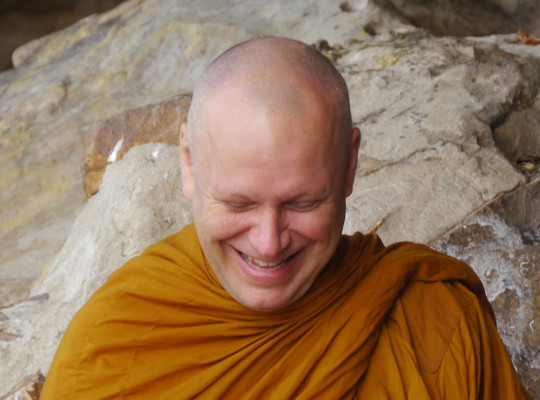
\includegraphics{info.jpg}

Bhante Shravasti Dhammika was born in Australia and took his lower
ordination as a Theravada monk in India in 1976. He has written over 25
books. He lived and taught in Singapore where he was spiritual advisor
to the Buddha Dhamma Mandala Society. In 2017 he moved back to Australia
and still continues to write about the Dhamma.
